% Latex header for doxygen 1.8.13
\documentclass[twoside]{book}
% Packages required by doxygen
\usepackage{fixltx2e}
\usepackage{calc}
\usepackage{doxygen}
\usepackage[export]{adjustbox} % also loads graphicx
\usepackage{graphicx}
\usepackage[utf8]{inputenc}
\usepackage{CJKutf8}
\usepackage{makeidx}
\usepackage{multicol}
\usepackage{multirow}
\PassOptionsToPackage{warn}{textcomp}
\usepackage{textcomp}
\usepackage[nointegrals]{wasysym}
\usepackage[table]{xcolor}
% Font selection
\usepackage[T1]{fontenc}
\usepackage[scaled=.90]{helvet}
\usepackage{courier}
\usepackage{amssymb}
\usepackage{sectsty}
\renewcommand{\familydefault}{\sfdefault}
\allsectionsfont{%
  \fontseries{bc}\selectfont%
  \color{darkgray}%
}
\renewcommand{\DoxyLabelFont}{%
  \fontseries{bc}\selectfont%
  \color{darkgray}%
}
\newcommand{\+}{\discretionary{\mbox{\scriptsize$\hookleftarrow$}}{}{}}
% Page & text layout
\usepackage{geometry}
\geometry{%
  a4paper,%
  top=2.5cm,%
  bottom=2.5cm,%
  left=2.5cm,%
  right=2.5cm%
}
\tolerance=750
\hfuzz=15pt
\hbadness=750
\setlength{\emergencystretch}{15pt}
\setlength{\parindent}{0cm}
\setlength{\parskip}{3ex plus 2ex minus 2ex}
\makeatletter
\renewcommand{\paragraph}{%
  \@startsection{paragraph}{4}{0ex}{-1.0ex}{1.0ex}{%
    \normalfont\normalsize\bfseries\SS@parafont%
  }%
}
\renewcommand{\subparagraph}{%
  \@startsection{subparagraph}{5}{0ex}{-1.0ex}{1.0ex}{%
    \normalfont\normalsize\bfseries\SS@subparafont%
  }%
}
\makeatother
% Headers & footers
\usepackage{fancyhdr}
\CJK{UTF8}{gbsn}
\pagestyle{fancyplain}
\fancyhead[LE]{\fancyplain{}{\bfseries\thepage}}
\fancyhead[CE]{\fancyplain{}{}}
\fancyhead[RE]{\fancyplain{}{\bfseries\leftmark}}
\fancyhead[LO]{\fancyplain{}{\bfseries\rightmark}}
\fancyhead[CO]{\fancyplain{}{}}
\fancyhead[RO]{\fancyplain{}{\bfseries\thepage}}
\fancyfoot[LE]{\fancyplain{}{\bfseries\scriptsize 震旦异构编译HALO平台}}
\fancyfoot[CE]{\fancyplain{}{\bfseries\scriptsize ODLA(Open Deep Learning API)}}
\fancyfoot[RE]{\fancyplain{}{\bfseries\scriptsize v0.5}}
\fancyfoot[LO]{\fancyplain{}{\bfseries\scriptsize 震旦异构编译HALO平台}}
\fancyfoot[CO]{\fancyplain{}{\bfseries\scriptsize ODLA(Open Deep Learning API)}}
\fancyfoot[RO]{\fancyplain{}{\bfseries\scriptsize v0.5}}
\renewcommand{\footrulewidth}{0.4pt}
\renewcommand{\chaptermark}[1]{%
  \markboth{#1}{}%
}
\renewcommand{\sectionmark}[1]{%
  \markright{\thesection\ #1}%
}
% Indices & bibliography
\usepackage{natbib}
\usepackage[titles]{tocloft}
\setcounter{tocdepth}{3}
\setcounter{secnumdepth}{5}
\makeindex
% Hyperlinks (required, but should be loaded last)
\usepackage{ifpdf}
\ifpdf
  \usepackage[pdftex,pagebackref=true]{hyperref}
\else
  \usepackage[ps2pdf,pagebackref=true]{hyperref}
\fi
\hypersetup{%
  colorlinks=true,%
  linkcolor=blue,%
  citecolor=blue,%
  unicode%
}
% Custom commands
\newcommand{\clearemptydoublepage}{%
  \newpage{\pagestyle{empty}\cleardoublepage}%
}
\usepackage{caption}
\captionsetup{labelsep=space,justification=centering,font={bf},singlelinecheck=off,skip=4pt,position=top}
%===== C O N T E N T S =====
\begin{document}
% Titlepage & ToC
\hypersetup{pageanchor=false,
             bookmarksnumbered=true,
             pdfencoding=unicode
            }
\pagenumbering{alph}
\begin{titlepage}
\vspace*{7cm}
\begin{center}%
{\Large Open Deep Learning API}\\
\vspace*{1cm}
{\large Version 0.5}\\
\vspace*{2cm}
{\large 震旦异构编译平台} \\
\end{center}
\end{titlepage}
\clearemptydoublepage
\pagenumbering{roman}
\tableofcontents
\clearemptydoublepage
\pagenumbering{arabic}
\hypersetup{pageanchor=true}
%--- Begin generated contents ---
\chapter{ODLA (Open Deep Learning API) API Reference}
\label{index}\hypertarget{index}{}\input{index}
\chapter{Data Structure Index}
\doxysection{Data Structures}
Here are the data structures with brief descriptions\+:\begin{DoxyCompactList}
\item\contentsline{section}{\mbox{\hyperlink{structodla__resource__location}{odla\+\_\+resource\+\_\+location}} \\*Resource location }{\pageref{structodla__resource__location}}{}
\item\contentsline{section}{\mbox{\hyperlink{structodla__scalar__value}{odla\+\_\+scalar\+\_\+value}} }{\pageref{structodla__scalar__value}}{}
\item\contentsline{section}{\mbox{\hyperlink{structodla__task}{odla\+\_\+task}} \\*Odla task definition }{\pageref{structodla__task}}{}
\item\contentsline{section}{\mbox{\hyperlink{structodla__value__ids}{odla\+\_\+value\+\_\+ids}} \\*Multiple value ids }{\pageref{structodla__value__ids}}{}
\item\contentsline{section}{\mbox{\hyperlink{structodla__value__quant__info}{odla\+\_\+value\+\_\+quant\+\_\+info}} \\*Quantization info for each odla value }{\pageref{structodla__value__quant__info}}{}
\item\contentsline{section}{\mbox{\hyperlink{structodla__value__shape}{odla\+\_\+value\+\_\+shape}} \\*Shape of value }{\pageref{structodla__value__shape}}{}
\item\contentsline{section}{\mbox{\hyperlink{structodla__value__type}{odla\+\_\+value\+\_\+type}} \\*Type of value }{\pageref{structodla__value__type}}{}
\item\contentsline{section}{\mbox{\hyperlink{structodla__values}{odla\+\_\+values}} \\*Multiple values }{\pageref{structodla__values}}{}
\end{DoxyCompactList}

\chapter{File Index}
\doxysection{File List}
Here is a list of all documented files with brief descriptions\+:\begin{DoxyCompactList}
\item\contentsline{section}{ODLA/\mbox{\hyperlink{odla_8h}{odla.\+h}} }{\pageref{odla_8h}}{}
\item\contentsline{section}{ODLA/\mbox{\hyperlink{odla__common_8h}{odla\+\_\+common.\+h}} }{\pageref{odla__common_8h}}{}
\item\contentsline{section}{ODLA/\mbox{\hyperlink{odla__compute_8h}{odla\+\_\+compute.\+h}} }{\pageref{odla__compute_8h}}{}
\item\contentsline{section}{ODLA/\mbox{\hyperlink{odla__device_8h}{odla\+\_\+device.\+h}} }{\pageref{odla__device_8h}}{}
\item\contentsline{section}{ODLA/\mbox{\hyperlink{odla__log_8h}{odla\+\_\+log.\+h}} }{\pageref{odla__log_8h}}{}
\item\contentsline{section}{ODLA/\mbox{\hyperlink{odla__memory_8h}{odla\+\_\+memory.\+h}} }{\pageref{odla__memory_8h}}{}
\item\contentsline{section}{ODLA/\mbox{\hyperlink{odla__ops_8h}{odla\+\_\+ops.\+h}} }{\pageref{odla__ops_8h}}{}
\item\contentsline{section}{ODLA/\mbox{\hyperlink{odla__profiler_8h}{odla\+\_\+profiler.\+h}} }{\pageref{odla__profiler_8h}}{}
\item\contentsline{section}{ODLA/\mbox{\hyperlink{odla__task_8h}{odla\+\_\+task.\+h}} }{\pageref{odla__task_8h}}{}
\item\contentsline{section}{ODLA/\mbox{\hyperlink{odla__value_8h}{odla\+\_\+value.\+h}} }{\pageref{odla__value_8h}}{}
\item\contentsline{section}{ODLA/\mbox{\hyperlink{odla__version_8h}{odla\+\_\+version.\+h}} }{\pageref{odla__version_8h}}{}
\item\contentsline{section}{ODLA/ops/\mbox{\hyperlink{odla__ops__basic_8h}{odla\+\_\+ops\+\_\+basic.\+h}} }{\pageref{odla__ops__basic_8h}}{}
\item\contentsline{section}{ODLA/ops/\mbox{\hyperlink{odla__ops__control__flow_8h}{odla\+\_\+ops\+\_\+control\+\_\+flow.\+h}} }{\pageref{odla__ops__control__flow_8h}}{}
\item\contentsline{section}{ODLA/ops/\mbox{\hyperlink{odla__ops__custom_8h}{odla\+\_\+ops\+\_\+custom.\+h}} }{\pageref{odla__ops__custom_8h}}{}
\item\contentsline{section}{ODLA/ops/\mbox{\hyperlink{odla__ops__math_8h}{odla\+\_\+ops\+\_\+math.\+h}} }{\pageref{odla__ops__math_8h}}{}
\item\contentsline{section}{ODLA/ops/\mbox{\hyperlink{odla__ops__nn_8h}{odla\+\_\+ops\+\_\+nn.\+h}} }{\pageref{odla__ops__nn_8h}}{}
\item\contentsline{section}{ODLA/ops/\mbox{\hyperlink{odla__ops__process_8h}{odla\+\_\+ops\+\_\+process.\+h}} }{\pageref{odla__ops__process_8h}}{}
\item\contentsline{section}{ODLA/ops/\mbox{\hyperlink{odla__ops__quantization_8h}{odla\+\_\+ops\+\_\+quantization.\+h}} }{\pageref{odla__ops__quantization_8h}}{}
\item\contentsline{section}{ODLA/ops/\mbox{\hyperlink{odla__ops__training_8h}{odla\+\_\+ops\+\_\+training.\+h}} }{\pageref{odla__ops__training_8h}}{}
\end{DoxyCompactList}

\chapter{Data Structure Documentation}
\hypertarget{structodla__task}{}\doxysection{odla\+\_\+task Struct Reference}
\label{structodla__task}\index{odla\_task@{odla\_task}}


odla task definition  




{\ttfamily \#include $<$odla\+\_\+task.\+h$>$}



Collaboration diagram for odla\+\_\+task\+:

\hypertarget{structodla__value__ids}{}\doxysection{odla\+\_\+value\+\_\+ids Struct Reference}
\label{structodla__value__ids}\index{odla\_value\_ids@{odla\_value\_ids}}


Multiple value ids.  




{\ttfamily \#include $<$odla\+\_\+value.\+h$>$}

\doxysubsection*{Data Fields}
\begin{DoxyCompactItemize}
\item 
\mbox{\hyperlink{odla__common_8h_acac65b5a20353d7f068ca61c6ab7569c}{odla\+\_\+size\+\_\+t}} \mbox{\hyperlink{structodla__value__ids_a501c149390cee1e8ded39313bb5ddde8}{size}}
\item 
\mbox{\hyperlink{odla__value_8h_a875459af53aca134ae1b1d82e971ec82}{odla\+\_\+value\+\_\+id}} \mbox{\hyperlink{structodla__value__ids_afe1dd6ff50cb0d266f8c81bf5c644f7a}{value\+\_\+ids}} \mbox{[}\mbox{\hyperlink{odla__value_8h_a7fd4a97be34945b2a2f70ddae3b30e23}{ODLA\+\_\+\+MAX\+\_\+\+OUTPUTS}}\mbox{]}
\end{DoxyCompactItemize}


\doxysubsection{Detailed Description}
Multiple value ids. 

Definition at line \mbox{\hyperlink{odla__value_8h_source_l00077}{77}} of file \mbox{\hyperlink{odla__value_8h_source}{odla\+\_\+value.\+h}}.



\doxysubsection{Field Documentation}
\mbox{\Hypertarget{structodla__value__ids_a501c149390cee1e8ded39313bb5ddde8}\label{structodla__value__ids_a501c149390cee1e8ded39313bb5ddde8}} 
\index{odla\_value\_ids@{odla\_value\_ids}!size@{size}}
\index{size@{size}!odla\_value\_ids@{odla\_value\_ids}}
\doxysubsubsection{\texorpdfstring{size}{size}}
{\footnotesize\ttfamily \mbox{\hyperlink{odla__common_8h_acac65b5a20353d7f068ca61c6ab7569c}{odla\+\_\+size\+\_\+t}} odla\+\_\+value\+\_\+ids\+::size}



Definition at line \mbox{\hyperlink{odla__value_8h_source_l00078}{78}} of file \mbox{\hyperlink{odla__value_8h_source}{odla\+\_\+value.\+h}}.

\mbox{\Hypertarget{structodla__value__ids_afe1dd6ff50cb0d266f8c81bf5c644f7a}\label{structodla__value__ids_afe1dd6ff50cb0d266f8c81bf5c644f7a}} 
\index{odla\_value\_ids@{odla\_value\_ids}!value\_ids@{value\_ids}}
\index{value\_ids@{value\_ids}!odla\_value\_ids@{odla\_value\_ids}}
\doxysubsubsection{\texorpdfstring{value\_ids}{value\_ids}}
{\footnotesize\ttfamily \mbox{\hyperlink{odla__value_8h_a875459af53aca134ae1b1d82e971ec82}{odla\+\_\+value\+\_\+id}} odla\+\_\+value\+\_\+ids\+::value\+\_\+ids\mbox{[}\mbox{\hyperlink{odla__value_8h_a7fd4a97be34945b2a2f70ddae3b30e23}{ODLA\+\_\+\+MAX\+\_\+\+OUTPUTS}}\mbox{]}}



Definition at line \mbox{\hyperlink{odla__value_8h_source_l00079}{79}} of file \mbox{\hyperlink{odla__value_8h_source}{odla\+\_\+value.\+h}}.



The documentation for this struct was generated from the following file\+:\begin{DoxyCompactItemize}
\item 
ODLA/\mbox{\hyperlink{odla__value_8h}{odla\+\_\+value.\+h}}\end{DoxyCompactItemize}

\input{structodla__value__quant__info}
\hypertarget{structodla__value__shape}{}\doxysection{odla\+\_\+value\+\_\+shape Struct Reference}
\label{structodla__value__shape}\index{odla\_value\_shape@{odla\_value\_shape}}


Shape of value.  




{\ttfamily \#include $<$odla\+\_\+value.\+h$>$}

\doxysubsection*{Data Fields}
\begin{DoxyCompactItemize}
\item 
\mbox{\hyperlink{odla__common_8h_a11711813c2dfcdbc8c94c8f73c47a203}{odla\+\_\+int32}} \mbox{\hyperlink{structodla__value__shape_a2de1ed7d13ccf5e77eea10f404475a56}{size}}
\item 
\mbox{\hyperlink{odla__common_8h_a4c8498c0bc04a3dc2e8683c1c9bd3aa9}{odla\+\_\+int64}} \mbox{\hyperlink{structodla__value__shape_a33778efb57bdfa6c2bb6fa4a5a25697a}{dims}} \mbox{[}\mbox{\hyperlink{odla__value_8h_a398ef994746c9294e4c1239f549a682f}{ODLA\+\_\+\+MAX\+\_\+\+DIMENSION}}\mbox{]}
\end{DoxyCompactItemize}


\doxysubsection{Detailed Description}
Shape of value. 

Definition at line \mbox{\hyperlink{odla__value_8h_source_l00051}{51}} of file \mbox{\hyperlink{odla__value_8h_source}{odla\+\_\+value.\+h}}.



\doxysubsection{Field Documentation}
\mbox{\Hypertarget{structodla__value__shape_a33778efb57bdfa6c2bb6fa4a5a25697a}\label{structodla__value__shape_a33778efb57bdfa6c2bb6fa4a5a25697a}} 
\index{odla\_value\_shape@{odla\_value\_shape}!dims@{dims}}
\index{dims@{dims}!odla\_value\_shape@{odla\_value\_shape}}
\doxysubsubsection{\texorpdfstring{dims}{dims}}
{\footnotesize\ttfamily \mbox{\hyperlink{odla__common_8h_a4c8498c0bc04a3dc2e8683c1c9bd3aa9}{odla\+\_\+int64}} odla\+\_\+value\+\_\+shape\+::dims\mbox{[}\mbox{\hyperlink{odla__value_8h_a398ef994746c9294e4c1239f549a682f}{ODLA\+\_\+\+MAX\+\_\+\+DIMENSION}}\mbox{]}}



Definition at line \mbox{\hyperlink{odla__value_8h_source_l00055}{55}} of file \mbox{\hyperlink{odla__value_8h_source}{odla\+\_\+value.\+h}}.

\mbox{\Hypertarget{structodla__value__shape_a2de1ed7d13ccf5e77eea10f404475a56}\label{structodla__value__shape_a2de1ed7d13ccf5e77eea10f404475a56}} 
\index{odla\_value\_shape@{odla\_value\_shape}!size@{size}}
\index{size@{size}!odla\_value\_shape@{odla\_value\_shape}}
\doxysubsubsection{\texorpdfstring{size}{size}}
{\footnotesize\ttfamily \mbox{\hyperlink{odla__common_8h_a11711813c2dfcdbc8c94c8f73c47a203}{odla\+\_\+int32}} odla\+\_\+value\+\_\+shape\+::size}



Definition at line \mbox{\hyperlink{odla__value_8h_source_l00053}{53}} of file \mbox{\hyperlink{odla__value_8h_source}{odla\+\_\+value.\+h}}.



The documentation for this struct was generated from the following file\+:\begin{DoxyCompactItemize}
\item 
ODLA/\mbox{\hyperlink{odla__value_8h}{odla\+\_\+value.\+h}}\end{DoxyCompactItemize}

\hypertarget{structodla__value__type}{}\doxysection{odla\+\_\+value\+\_\+type Struct Reference}
\label{structodla__value__type}\index{odla\_value\_type@{odla\_value\_type}}


Type of value.  




{\ttfamily \#include $<$odla\+\_\+value.\+h$>$}



Collaboration diagram for odla\+\_\+value\+\_\+type\+:
\nopagebreak
\begin{figure}[H]
\begin{center}
\leavevmode
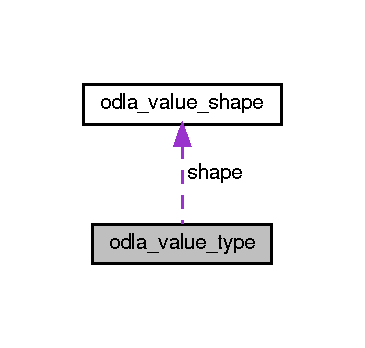
\includegraphics[width=175pt]{structodla__value__type__coll__graph}
\end{center}
\end{figure}
\doxysubsection*{Data Fields}
\begin{DoxyCompactItemize}
\item 
odla\+\_\+element\+\_\+type \mbox{\hyperlink{structodla__value__type_a926941f930d1de2f44be7767d40e3402}{element\+\_\+type}}
\item 
\mbox{\hyperlink{structodla__value__shape}{odla\+\_\+value\+\_\+shape}} \mbox{\hyperlink{structodla__value__type_a71e32dec2c65553cba0d3612f9facb0d}{shape}}
\end{DoxyCompactItemize}


\doxysubsection{Detailed Description}
Type of value. 

Definition at line \mbox{\hyperlink{odla__value_8h_source_l00059}{59}} of file \mbox{\hyperlink{odla__value_8h_source}{odla\+\_\+value.\+h}}.



\doxysubsection{Field Documentation}
\mbox{\Hypertarget{structodla__value__type_a926941f930d1de2f44be7767d40e3402}\label{structodla__value__type_a926941f930d1de2f44be7767d40e3402}} 
\index{odla\_value\_type@{odla\_value\_type}!element\_type@{element\_type}}
\index{element\_type@{element\_type}!odla\_value\_type@{odla\_value\_type}}
\doxysubsubsection{\texorpdfstring{element\_type}{element\_type}}
{\footnotesize\ttfamily odla\+\_\+element\+\_\+type odla\+\_\+value\+\_\+type\+::element\+\_\+type}



Definition at line \mbox{\hyperlink{odla__value_8h_source_l00060}{60}} of file \mbox{\hyperlink{odla__value_8h_source}{odla\+\_\+value.\+h}}.

\mbox{\Hypertarget{structodla__value__type_a71e32dec2c65553cba0d3612f9facb0d}\label{structodla__value__type_a71e32dec2c65553cba0d3612f9facb0d}} 
\index{odla\_value\_type@{odla\_value\_type}!shape@{shape}}
\index{shape@{shape}!odla\_value\_type@{odla\_value\_type}}
\doxysubsubsection{\texorpdfstring{shape}{shape}}
{\footnotesize\ttfamily \mbox{\hyperlink{structodla__value__shape}{odla\+\_\+value\+\_\+shape}} odla\+\_\+value\+\_\+type\+::shape}



Definition at line \mbox{\hyperlink{odla__value_8h_source_l00061}{61}} of file \mbox{\hyperlink{odla__value_8h_source}{odla\+\_\+value.\+h}}.



The documentation for this struct was generated from the following file\+:\begin{DoxyCompactItemize}
\item 
ODLA/\mbox{\hyperlink{odla__value_8h}{odla\+\_\+value.\+h}}\end{DoxyCompactItemize}

\hypertarget{structodla__values}{}\doxysection{odla\+\_\+values Struct Reference}
\label{structodla__values}\index{odla\_values@{odla\_values}}


Multiple values.  




{\ttfamily \#include $<$odla\+\_\+value.\+h$>$}

\doxysubsection*{Data Fields}
\begin{DoxyCompactItemize}
\item 
\mbox{\hyperlink{odla__common_8h_acac65b5a20353d7f068ca61c6ab7569c}{odla\+\_\+size\+\_\+t}} \mbox{\hyperlink{structodla__values_a6e41ada4101881ea20fea4c64ea28ac3}{size}}
\item 
\mbox{\hyperlink{odla__value_8h_ace8591dbfa7d6ec7c38533286be8490b}{odla\+\_\+value}} \mbox{\hyperlink{structodla__values_a7ce0300f9688e94931eb9b6a05f86d59}{values}} \mbox{[}\mbox{\hyperlink{odla__value_8h_a7fd4a97be34945b2a2f70ddae3b30e23}{ODLA\+\_\+\+MAX\+\_\+\+OUTPUTS}}\mbox{]}
\end{DoxyCompactItemize}


\doxysubsection{Detailed Description}
Multiple values. 

Definition at line \mbox{\hyperlink{odla__value_8h_source_l00068}{68}} of file \mbox{\hyperlink{odla__value_8h_source}{odla\+\_\+value.\+h}}.



\doxysubsection{Field Documentation}
\mbox{\Hypertarget{structodla__values_a6e41ada4101881ea20fea4c64ea28ac3}\label{structodla__values_a6e41ada4101881ea20fea4c64ea28ac3}} 
\index{odla\_values@{odla\_values}!size@{size}}
\index{size@{size}!odla\_values@{odla\_values}}
\doxysubsubsection{\texorpdfstring{size}{size}}
{\footnotesize\ttfamily \mbox{\hyperlink{odla__common_8h_acac65b5a20353d7f068ca61c6ab7569c}{odla\+\_\+size\+\_\+t}} odla\+\_\+values\+::size}



Definition at line \mbox{\hyperlink{odla__value_8h_source_l00069}{69}} of file \mbox{\hyperlink{odla__value_8h_source}{odla\+\_\+value.\+h}}.

\mbox{\Hypertarget{structodla__values_a7ce0300f9688e94931eb9b6a05f86d59}\label{structodla__values_a7ce0300f9688e94931eb9b6a05f86d59}} 
\index{odla\_values@{odla\_values}!values@{values}}
\index{values@{values}!odla\_values@{odla\_values}}
\doxysubsubsection{\texorpdfstring{values}{values}}
{\footnotesize\ttfamily \mbox{\hyperlink{odla__value_8h_ace8591dbfa7d6ec7c38533286be8490b}{odla\+\_\+value}} odla\+\_\+values\+::values\mbox{[}\mbox{\hyperlink{odla__value_8h_a7fd4a97be34945b2a2f70ddae3b30e23}{ODLA\+\_\+\+MAX\+\_\+\+OUTPUTS}}\mbox{]}}



Definition at line \mbox{\hyperlink{odla__value_8h_source_l00070}{70}} of file \mbox{\hyperlink{odla__value_8h_source}{odla\+\_\+value.\+h}}.



The documentation for this struct was generated from the following file\+:\begin{DoxyCompactItemize}
\item 
ODLA/\mbox{\hyperlink{odla__value_8h}{odla\+\_\+value.\+h}}\end{DoxyCompactItemize}

\chapter{File Documentation}
\input{odla_8h}
\hypertarget{odla_8h_source}{}\doxysection{odla.\+h}
\label{odla_8h_source}\index{ODLA/odla.h@{ODLA/odla.h}}
\mbox{\hyperlink{odla_8h}{Go to the documentation of this file.}}
\begin{DoxyCode}{0}
\DoxyCodeLine{\Hypertarget{odla_8h_source_l00001}00001 \textcolor{comment}{//===-\/ odla.h -\/-\/-\/-\/-\/-\/-\/-\/-\/-\/-\/-\/-\/-\/-\/-\/-\/-\/-\/-\/-\/-\/-\/-\/-\/-\/-\/-\/-\/-\/-\/-\/-\/-\/-\/-\/-\/-\/-\/-\/-\/-\/-\/-\/-\/-\/-\/-\/-\/-\/-\/-\/-\/-\/-\/-\/-\/-\/-\/-\/-\/===//}}
\DoxyCodeLine{\Hypertarget{odla_8h_source_l00002}00002 \textcolor{comment}{//}}
\DoxyCodeLine{\Hypertarget{odla_8h_source_l00003}00003 \textcolor{comment}{// Copyright (C) 2019-\/2020 Alibaba Group Holding Limited.}}
\DoxyCodeLine{\Hypertarget{odla_8h_source_l00004}00004 \textcolor{comment}{//}}
\DoxyCodeLine{\Hypertarget{odla_8h_source_l00005}00005 \textcolor{comment}{// Licensed under the Apache License, Version 2.0 (the "{}License"{});}}
\DoxyCodeLine{\Hypertarget{odla_8h_source_l00006}00006 \textcolor{comment}{// you may not use this file except in compliance with the License.}}
\DoxyCodeLine{\Hypertarget{odla_8h_source_l00007}00007 \textcolor{comment}{// You may obtain a copy of the License at}}
\DoxyCodeLine{\Hypertarget{odla_8h_source_l00008}00008 \textcolor{comment}{//}}
\DoxyCodeLine{\Hypertarget{odla_8h_source_l00009}00009 \textcolor{comment}{//   http://www.apache.org/licenses/LICENSE-\/2.0}}
\DoxyCodeLine{\Hypertarget{odla_8h_source_l00010}00010 \textcolor{comment}{//}}
\DoxyCodeLine{\Hypertarget{odla_8h_source_l00011}00011 \textcolor{comment}{// Unless required by applicable law or agreed to in writing, software}}
\DoxyCodeLine{\Hypertarget{odla_8h_source_l00012}00012 \textcolor{comment}{// distributed under the License is distributed on an "{}AS IS"{} BASIS,}}
\DoxyCodeLine{\Hypertarget{odla_8h_source_l00013}00013 \textcolor{comment}{// WITHOUT WARRANTIES OR CONDITIONS OF ANY KIND, either express or implied.}}
\DoxyCodeLine{\Hypertarget{odla_8h_source_l00014}00014 \textcolor{comment}{// See the License for the specific language governing permissions and}}
\DoxyCodeLine{\Hypertarget{odla_8h_source_l00015}00015 \textcolor{comment}{// limitations under the License.}}
\DoxyCodeLine{\Hypertarget{odla_8h_source_l00016}00016 \textcolor{comment}{// =============================================================================}}
\DoxyCodeLine{\Hypertarget{odla_8h_source_l00017}00017 }
\DoxyCodeLine{\Hypertarget{odla_8h_source_l00018}00018 \textcolor{preprocessor}{\#ifndef \_ODLA\_H\_}}
\DoxyCodeLine{\Hypertarget{odla_8h_source_l00019}00019 \textcolor{preprocessor}{\#define \_ODLA\_H\_}}
\DoxyCodeLine{\Hypertarget{odla_8h_source_l00020}00020 }
\DoxyCodeLine{\Hypertarget{odla_8h_source_l00021}00021 \textcolor{preprocessor}{\#include <\mbox{\hyperlink{odla__common_8h}{ODLA/odla\_common.h}}>}}
\DoxyCodeLine{\Hypertarget{odla_8h_source_l00022}00022 \textcolor{preprocessor}{\#include <\mbox{\hyperlink{odla__compute_8h}{ODLA/odla\_compute.h}}>}}
\DoxyCodeLine{\Hypertarget{odla_8h_source_l00023}00023 \textcolor{preprocessor}{\#include <\mbox{\hyperlink{odla__device_8h}{ODLA/odla\_device.h}}>}}
\DoxyCodeLine{\Hypertarget{odla_8h_source_l00024}00024 \textcolor{preprocessor}{\#include <\mbox{\hyperlink{odla__log_8h}{ODLA/odla\_log.h}}>}}
\DoxyCodeLine{\Hypertarget{odla_8h_source_l00025}00025 \textcolor{preprocessor}{\#include <\mbox{\hyperlink{odla__memory_8h}{ODLA/odla\_memory.h}}>}}
\DoxyCodeLine{\Hypertarget{odla_8h_source_l00026}00026 \textcolor{preprocessor}{\#include <\mbox{\hyperlink{odla__ops_8h}{ODLA/odla\_ops.h}}>}}
\DoxyCodeLine{\Hypertarget{odla_8h_source_l00027}00027 \textcolor{preprocessor}{\#include <\mbox{\hyperlink{odla__profiler_8h}{ODLA/odla\_profiler.h}}>}}
\DoxyCodeLine{\Hypertarget{odla_8h_source_l00028}00028 \textcolor{preprocessor}{\#include <\mbox{\hyperlink{odla__task_8h}{ODLA/odla\_task.h}}>}}
\DoxyCodeLine{\Hypertarget{odla_8h_source_l00029}00029 \textcolor{preprocessor}{\#include <\mbox{\hyperlink{odla__value_8h}{ODLA/odla\_value.h}}>}}
\DoxyCodeLine{\Hypertarget{odla_8h_source_l00030}00030 \textcolor{preprocessor}{\#include <\mbox{\hyperlink{odla__version_8h}{ODLA/odla\_version.h}}>}}
\DoxyCodeLine{\Hypertarget{odla_8h_source_l00031}00031 }
\DoxyCodeLine{\Hypertarget{odla_8h_source_l00039}00039 \textcolor{preprocessor}{\#ifdef \_\_cplusplus}}
\DoxyCodeLine{\Hypertarget{odla_8h_source_l00040}00040 \textcolor{keyword}{extern} \textcolor{stringliteral}{"{}C"{}} \{}
\DoxyCodeLine{\Hypertarget{odla_8h_source_l00041}00041 \textcolor{preprocessor}{\#endif}}
\DoxyCodeLine{\Hypertarget{odla_8h_source_l00042}00042 }
\DoxyCodeLine{\Hypertarget{odla_8h_source_l00043}00043 \textcolor{preprocessor}{\#ifdef \_\_cplusplus}}
\DoxyCodeLine{\Hypertarget{odla_8h_source_l00044}00044 \} \textcolor{comment}{// C extern}}
\DoxyCodeLine{\Hypertarget{odla_8h_source_l00045}00045 \textcolor{preprocessor}{\#endif}}
\DoxyCodeLine{\Hypertarget{odla_8h_source_l00046}00046 }
\DoxyCodeLine{\Hypertarget{odla_8h_source_l00047}00047 \textcolor{preprocessor}{\#endif }\textcolor{comment}{// \_ODLA\_H\_}}

\end{DoxyCode}

\hypertarget{odla__common_8h}{}\doxysection{ODLA/odla\+\_\+common.h File Reference}
\label{odla__common_8h}\index{ODLA/odla\_common.h@{ODLA/odla\_common.h}}
\doxysubsection*{Macros}
\begin{DoxyCompactItemize}
\item 
\#define \mbox{\hyperlink{odla__common_8h_a070d2ce7b6bb7e5c05602aa8c308d0c4}{NULL}}~((void$\ast$)0)
\item 
\#define \mbox{\hyperlink{odla__common_8h_a1f9123e77ab174e483a7f307eb9c264e}{ODLA\+\_\+\+API\+\_\+\+EXPORT}}
\begin{DoxyCompactList}\small\item\em API export directives. \end{DoxyCompactList}\item 
\#define \mbox{\hyperlink{odla__common_8h_a115004e03b7bafa9bd7ab433afc7ac5f}{ODLA\+\_\+\+API\+\_\+\+CALL}}
\end{DoxyCompactItemize}
\doxysubsection*{Typedefs}
\begin{DoxyCompactItemize}
\item 
typedef \+\_\+\+\_\+\+INT8\+\_\+\+TYPE\+\_\+\+\_\+ \mbox{\hyperlink{odla__common_8h_ab759367dbc391f2a4c1ef47fc12640d1}{odla\+\_\+int8}}
\item 
typedef \+\_\+\+\_\+\+INT16\+\_\+\+TYPE\+\_\+\+\_\+ \mbox{\hyperlink{odla__common_8h_a6fecbc127ee239fc550a1568bd0f44c2}{odla\+\_\+int16}}
\item 
typedef \+\_\+\+\_\+\+INT32\+\_\+\+TYPE\+\_\+\+\_\+ \mbox{\hyperlink{odla__common_8h_a11711813c2dfcdbc8c94c8f73c47a203}{odla\+\_\+int32}}
\item 
typedef \+\_\+\+\_\+\+INT64\+\_\+\+TYPE\+\_\+\+\_\+ \mbox{\hyperlink{odla__common_8h_a4c8498c0bc04a3dc2e8683c1c9bd3aa9}{odla\+\_\+int64}}
\item 
typedef \+\_\+\+\_\+\+UINT8\+\_\+\+TYPE\+\_\+\+\_\+ \mbox{\hyperlink{odla__common_8h_a865438a9ae649ef089e0e577dabc280d}{odla\+\_\+uint8}}
\item 
typedef \+\_\+\+\_\+\+UINT16\+\_\+\+TYPE\+\_\+\+\_\+ \mbox{\hyperlink{odla__common_8h_a06050332dcc769101e4de49f7ccc2139}{odla\+\_\+uint16}}
\item 
typedef \+\_\+\+\_\+\+UINT32\+\_\+\+TYPE\+\_\+\+\_\+ \mbox{\hyperlink{odla__common_8h_a6b80c6921b4b4e20c95df868e20c8afd}{odla\+\_\+uint32}}
\item 
typedef \+\_\+\+\_\+\+UINT64\+\_\+\+TYPE\+\_\+\+\_\+ \mbox{\hyperlink{odla__common_8h_aeb84ef9d7f788f94b03b14ad3517b374}{odla\+\_\+uint64}}
\item 
typedef \+\_\+\+\_\+\+INT8\+\_\+\+TYPE\+\_\+\+\_\+ \mbox{\hyperlink{odla__common_8h_aacf1be22ddf1341e1d39369fd39c2f72}{odla\+\_\+qint8}}
\item 
typedef \+\_\+\+\_\+\+INT16\+\_\+\+TYPE\+\_\+\+\_\+ \mbox{\hyperlink{odla__common_8h_aaaa5d01bda022f8b6f4ff38680741426}{odla\+\_\+qint16}}
\item 
typedef \+\_\+\+\_\+\+INT32\+\_\+\+TYPE\+\_\+\+\_\+ \mbox{\hyperlink{odla__common_8h_a1766e33e280d3cf1638c892d9246b47d}{odla\+\_\+qint32}}
\item 
typedef \+\_\+\+\_\+\+INT64\+\_\+\+TYPE\+\_\+\+\_\+ \mbox{\hyperlink{odla__common_8h_ae11db7721a08fec274632164c0afd399}{odla\+\_\+qint64}}
\item 
typedef \+\_\+\+\_\+\+UINT8\+\_\+\+TYPE\+\_\+\+\_\+ \mbox{\hyperlink{odla__common_8h_a47681b75cefcd1e2355ef155beb6931b}{odla\+\_\+quint8}}
\item 
typedef \+\_\+\+\_\+\+UINT16\+\_\+\+TYPE\+\_\+\+\_\+ \mbox{\hyperlink{odla__common_8h_a24af12d9854e5945e989ce9c660e3faf}{odla\+\_\+quint16}}
\item 
typedef \+\_\+\+\_\+\+UINT32\+\_\+\+TYPE\+\_\+\+\_\+ \mbox{\hyperlink{odla__common_8h_ac7491c5982654776eb48710a97c33e75}{odla\+\_\+quint32}}
\item 
typedef \+\_\+\+\_\+\+UINT64\+\_\+\+TYPE\+\_\+\+\_\+ \mbox{\hyperlink{odla__common_8h_a02772eefb47a8a4219be7e23d56cbe24}{odla\+\_\+quint64}}
\item 
typedef \+\_\+\+\_\+\+UINT16\+\_\+\+TYPE\+\_\+\+\_\+ \mbox{\hyperlink{odla__common_8h_a64ee51987605659050cbe1ef64941f1d}{odla\+\_\+float16}}
\item 
typedef \+\_\+\+\_\+\+UINT16\+\_\+\+TYPE\+\_\+\+\_\+ \mbox{\hyperlink{odla__common_8h_ac44ebee1dd76490c3192d430311c0f1b}{odla\+\_\+bfloat16}}
\item 
typedef float \mbox{\hyperlink{odla__common_8h_aeaf2b4ed87e14f5bbf792ab782aa73f5}{odla\+\_\+float32}}
\item 
typedef double \mbox{\hyperlink{odla__common_8h_a956bdf1765e13ccacb04cbf02de7d0b3}{odla\+\_\+float64}}
\item 
typedef \mbox{\hyperlink{odla__common_8h_a6b80c6921b4b4e20c95df868e20c8afd}{odla\+\_\+uint32}} \mbox{\hyperlink{odla__common_8h_a86f265601c0773152f4e193a8614c0ac}{odla\+\_\+bool}}
\item 
typedef char \mbox{\hyperlink{odla__common_8h_a70ab5c97f8e2150ab1c252e6fa33d38b}{odla\+\_\+char}}
\begin{DoxyCompactList}\small\item\em char \end{DoxyCompactList}\item 
typedef \+\_\+\+\_\+\+SIZE\+\_\+\+TYPE\+\_\+\+\_\+ \mbox{\hyperlink{odla__common_8h_acac65b5a20353d7f068ca61c6ab7569c}{odla\+\_\+size\+\_\+t}}
\begin{DoxyCompactList}\small\item\em size\+\_\+t \end{DoxyCompactList}\item 
typedef void \mbox{\hyperlink{odla__common_8h_ada3e0e93ebd03f1f5fe3ff21655cdb11}{odla\+\_\+void}}
\begin{DoxyCompactList}\small\item\em void \end{DoxyCompactList}\end{DoxyCompactItemize}
\doxysubsection*{Enumerations}
\begin{DoxyCompactItemize}
\item 
enum {\bfseries odla\+\_\+element\+\_\+type} \{ \newline
{\bfseries ODLA\+\_\+\+INT8}
, {\bfseries ODLA\+\_\+\+INT16}
, {\bfseries ODLA\+\_\+\+INT32}
, {\bfseries ODLA\+\_\+\+INT64}
, \newline
{\bfseries ODLA\+\_\+\+UINT8}
, {\bfseries ODLA\+\_\+\+UINT16}
, {\bfseries ODLA\+\_\+\+UINT32}
, {\bfseries ODLA\+\_\+\+UINT64}
, \newline
{\bfseries ODLA\+\_\+\+QINT8}
, {\bfseries ODLA\+\_\+\+QINT16}
, {\bfseries ODLA\+\_\+\+QINT32}
, {\bfseries ODLA\+\_\+\+QINT64}
, \newline
{\bfseries ODLA\+\_\+\+QUINT8}
, {\bfseries ODLA\+\_\+\+QUINT16}
, {\bfseries ODLA\+\_\+\+QUINT32}
, {\bfseries ODLA\+\_\+\+QUINT64}
, \newline
{\bfseries ODLA\+\_\+\+FLOAT16}
, {\bfseries ODLA\+\_\+\+BFLOAT16}
, {\bfseries ODLA\+\_\+\+FLOAT32}
, {\bfseries ODLA\+\_\+\+FLOAT64}
, \newline
{\bfseries ODLA\+\_\+\+BOOL}
 \}
\item 
enum \mbox{\hyperlink{odla__common_8h_a32d12bc3360c8b8891c225a703f7db29}{odla\+\_\+status}} \{ \newline
{\bfseries ODLA\+\_\+\+SUCCESS}
, \mbox{\hyperlink{odla__common_8h_a32d12bc3360c8b8891c225a703f7db29a6d455c06ecdf45fe88b1e126ca213087}{ODLA\+\_\+\+DL\+\_\+\+ERROR}}
, {\bfseries ODLA\+\_\+\+FILE\+\_\+\+NOT\+\_\+\+EXIST}
, \mbox{\hyperlink{odla__common_8h_a32d12bc3360c8b8891c225a703f7db29a5b894b19f9456cae708edc778f63218f}{ODLA\+\_\+\+INVALID\+\_\+\+PARAM}}
, \newline
\mbox{\hyperlink{odla__common_8h_a32d12bc3360c8b8891c225a703f7db29a3bbe59e41327500a9a709ae05af34dd1}{ODLA\+\_\+\+MEM\+\_\+\+ERROR}}
, {\bfseries ODLA\+\_\+\+UNSUPPORTED\+\_\+\+DATATYPE}
, {\bfseries ODLA\+\_\+\+UNSUPPORTED\+\_\+\+DEVICE\+\_\+\+TYPE}
, \mbox{\hyperlink{odla__common_8h_a32d12bc3360c8b8891c225a703f7db29abb64d0b5146c0236d571cb897384853e}{ODLA\+\_\+\+UNSUPPORTED\+\_\+\+OP}}
, \newline
\mbox{\hyperlink{odla__common_8h_a32d12bc3360c8b8891c225a703f7db29a2a2087e4e487e8ec867e356bdcc95f00}{ODLA\+\_\+\+TIMEOUT}}
, \mbox{\hyperlink{odla__common_8h_a32d12bc3360c8b8891c225a703f7db29a0c19e9d42ae016f5b9dc9a7054077d13}{ODLA\+\_\+\+INTERNAL\+\_\+\+LOGIC\+\_\+\+ERR}}
, \mbox{\hyperlink{odla__common_8h_a32d12bc3360c8b8891c225a703f7db29a78d98eb3ea302582a487afa76c9f1344}{ODLA\+\_\+\+RECOVERABLE\+\_\+\+ERR}}
, \mbox{\hyperlink{odla__common_8h_a32d12bc3360c8b8891c225a703f7db29a4f2a588c748813827894ececed6a4547}{ODLA\+\_\+\+PARTITION\+\_\+\+RESET}}
, \newline
{\bfseries ODLA\+\_\+\+FULL\+\_\+\+RESET}
, \mbox{\hyperlink{odla__common_8h_a32d12bc3360c8b8891c225a703f7db29a7f249f9bdd98e4745333b2c83ac73a7c}{ODLA\+\_\+\+UNRECOVERABLE\+\_\+\+ERR}}
, {\bfseries ODLA\+\_\+\+FAILURE}
 \}
\begin{DoxyCompactList}\small\item\em Return status. \end{DoxyCompactList}\end{DoxyCompactItemize}


\doxysubsection{Detailed Description}
This file defines the ODLA basic common types. 

Definition in file \mbox{\hyperlink{odla__common_8h_source}{odla\+\_\+common.\+h}}.



\doxysubsection{Macro Definition Documentation}
\mbox{\Hypertarget{odla__common_8h_a070d2ce7b6bb7e5c05602aa8c308d0c4}\label{odla__common_8h_a070d2ce7b6bb7e5c05602aa8c308d0c4}} 
\index{odla\_common.h@{odla\_common.h}!NULL@{NULL}}
\index{NULL@{NULL}!odla\_common.h@{odla\_common.h}}
\doxysubsubsection{\texorpdfstring{NULL}{NULL}}
{\footnotesize\ttfamily \#define NULL~((void$\ast$)0)}



Definition at line \mbox{\hyperlink{odla__common_8h_source_l00094}{94}} of file \mbox{\hyperlink{odla__common_8h_source}{odla\+\_\+common.\+h}}.

\mbox{\Hypertarget{odla__common_8h_a115004e03b7bafa9bd7ab433afc7ac5f}\label{odla__common_8h_a115004e03b7bafa9bd7ab433afc7ac5f}} 
\index{odla\_common.h@{odla\_common.h}!ODLA\_API\_CALL@{ODLA\_API\_CALL}}
\index{ODLA\_API\_CALL@{ODLA\_API\_CALL}!odla\_common.h@{odla\_common.h}}
\doxysubsubsection{\texorpdfstring{ODLA\_API\_CALL}{ODLA\_API\_CALL}}
{\footnotesize\ttfamily \#define ODLA\+\_\+\+API\+\_\+\+CALL}



Definition at line \mbox{\hyperlink{odla__common_8h_source_l00170}{170}} of file \mbox{\hyperlink{odla__common_8h_source}{odla\+\_\+common.\+h}}.

\mbox{\Hypertarget{odla__common_8h_a1f9123e77ab174e483a7f307eb9c264e}\label{odla__common_8h_a1f9123e77ab174e483a7f307eb9c264e}} 
\index{odla\_common.h@{odla\_common.h}!ODLA\_API\_EXPORT@{ODLA\_API\_EXPORT}}
\index{ODLA\_API\_EXPORT@{ODLA\_API\_EXPORT}!odla\_common.h@{odla\_common.h}}
\doxysubsubsection{\texorpdfstring{ODLA\_API\_EXPORT}{ODLA\_API\_EXPORT}}
{\footnotesize\ttfamily \#define ODLA\+\_\+\+API\+\_\+\+EXPORT}



API export directives. 



Definition at line \mbox{\hyperlink{odla__common_8h_source_l00169}{169}} of file \mbox{\hyperlink{odla__common_8h_source}{odla\+\_\+common.\+h}}.



\doxysubsection{Typedef Documentation}
\mbox{\Hypertarget{odla__common_8h_ac44ebee1dd76490c3192d430311c0f1b}\label{odla__common_8h_ac44ebee1dd76490c3192d430311c0f1b}} 
\index{odla\_common.h@{odla\_common.h}!odla\_bfloat16@{odla\_bfloat16}}
\index{odla\_bfloat16@{odla\_bfloat16}!odla\_common.h@{odla\_common.h}}
\doxysubsubsection{\texorpdfstring{odla\_bfloat16}{odla\_bfloat16}}
{\footnotesize\ttfamily typedef \+\_\+\+\_\+\+UINT16\+\_\+\+TYPE\+\_\+\+\_\+ \mbox{\hyperlink{odla__common_8h_ac44ebee1dd76490c3192d430311c0f1b}{odla\+\_\+bfloat16}}}

16-\/bit brain floating point type 

Definition at line \mbox{\hyperlink{odla__common_8h_source_l00088}{88}} of file \mbox{\hyperlink{odla__common_8h_source}{odla\+\_\+common.\+h}}.

\mbox{\Hypertarget{odla__common_8h_a86f265601c0773152f4e193a8614c0ac}\label{odla__common_8h_a86f265601c0773152f4e193a8614c0ac}} 
\index{odla\_common.h@{odla\_common.h}!odla\_bool@{odla\_bool}}
\index{odla\_bool@{odla\_bool}!odla\_common.h@{odla\_common.h}}
\doxysubsubsection{\texorpdfstring{odla\_bool}{odla\_bool}}
{\footnotesize\ttfamily typedef \mbox{\hyperlink{odla__common_8h_a6b80c6921b4b4e20c95df868e20c8afd}{odla\+\_\+uint32}} \mbox{\hyperlink{odla__common_8h_a86f265601c0773152f4e193a8614c0ac}{odla\+\_\+bool}}}

boolean type 

Definition at line \mbox{\hyperlink{odla__common_8h_source_l00097}{97}} of file \mbox{\hyperlink{odla__common_8h_source}{odla\+\_\+common.\+h}}.

\mbox{\Hypertarget{odla__common_8h_a70ab5c97f8e2150ab1c252e6fa33d38b}\label{odla__common_8h_a70ab5c97f8e2150ab1c252e6fa33d38b}} 
\index{odla\_common.h@{odla\_common.h}!odla\_char@{odla\_char}}
\index{odla\_char@{odla\_char}!odla\_common.h@{odla\_common.h}}
\doxysubsubsection{\texorpdfstring{odla\_char}{odla\_char}}
{\footnotesize\ttfamily typedef char \mbox{\hyperlink{odla__common_8h_a70ab5c97f8e2150ab1c252e6fa33d38b}{odla\+\_\+char}}}



char 



Definition at line \mbox{\hyperlink{odla__common_8h_source_l00128}{128}} of file \mbox{\hyperlink{odla__common_8h_source}{odla\+\_\+common.\+h}}.

\mbox{\Hypertarget{odla__common_8h_a64ee51987605659050cbe1ef64941f1d}\label{odla__common_8h_a64ee51987605659050cbe1ef64941f1d}} 
\index{odla\_common.h@{odla\_common.h}!odla\_float16@{odla\_float16}}
\index{odla\_float16@{odla\_float16}!odla\_common.h@{odla\_common.h}}
\doxysubsubsection{\texorpdfstring{odla\_float16}{odla\_float16}}
{\footnotesize\ttfamily typedef \+\_\+\+\_\+\+UINT16\+\_\+\+TYPE\+\_\+\+\_\+ \mbox{\hyperlink{odla__common_8h_a64ee51987605659050cbe1ef64941f1d}{odla\+\_\+float16}}}

16-\/bit floating point type 

Definition at line \mbox{\hyperlink{odla__common_8h_source_l00087}{87}} of file \mbox{\hyperlink{odla__common_8h_source}{odla\+\_\+common.\+h}}.

\mbox{\Hypertarget{odla__common_8h_aeaf2b4ed87e14f5bbf792ab782aa73f5}\label{odla__common_8h_aeaf2b4ed87e14f5bbf792ab782aa73f5}} 
\index{odla\_common.h@{odla\_common.h}!odla\_float32@{odla\_float32}}
\index{odla\_float32@{odla\_float32}!odla\_common.h@{odla\_common.h}}
\doxysubsubsection{\texorpdfstring{odla\_float32}{odla\_float32}}
{\footnotesize\ttfamily typedef float \mbox{\hyperlink{odla__common_8h_aeaf2b4ed87e14f5bbf792ab782aa73f5}{odla\+\_\+float32}}}

32-\/bit floating point type 

Definition at line \mbox{\hyperlink{odla__common_8h_source_l00089}{89}} of file \mbox{\hyperlink{odla__common_8h_source}{odla\+\_\+common.\+h}}.

\mbox{\Hypertarget{odla__common_8h_a956bdf1765e13ccacb04cbf02de7d0b3}\label{odla__common_8h_a956bdf1765e13ccacb04cbf02de7d0b3}} 
\index{odla\_common.h@{odla\_common.h}!odla\_float64@{odla\_float64}}
\index{odla\_float64@{odla\_float64}!odla\_common.h@{odla\_common.h}}
\doxysubsubsection{\texorpdfstring{odla\_float64}{odla\_float64}}
{\footnotesize\ttfamily typedef double \mbox{\hyperlink{odla__common_8h_a956bdf1765e13ccacb04cbf02de7d0b3}{odla\+\_\+float64}}}

64-\/bit floating point type 

Definition at line \mbox{\hyperlink{odla__common_8h_source_l00090}{90}} of file \mbox{\hyperlink{odla__common_8h_source}{odla\+\_\+common.\+h}}.

\mbox{\Hypertarget{odla__common_8h_a6fecbc127ee239fc550a1568bd0f44c2}\label{odla__common_8h_a6fecbc127ee239fc550a1568bd0f44c2}} 
\index{odla\_common.h@{odla\_common.h}!odla\_int16@{odla\_int16}}
\index{odla\_int16@{odla\_int16}!odla\_common.h@{odla\_common.h}}
\doxysubsubsection{\texorpdfstring{odla\_int16}{odla\_int16}}
{\footnotesize\ttfamily typedef \+\_\+\+\_\+\+INT16\+\_\+\+TYPE\+\_\+\+\_\+ \mbox{\hyperlink{odla__common_8h_a6fecbc127ee239fc550a1568bd0f44c2}{odla\+\_\+int16}}}

16-\/bit signed integer type 

Definition at line \mbox{\hyperlink{odla__common_8h_source_l00064}{64}} of file \mbox{\hyperlink{odla__common_8h_source}{odla\+\_\+common.\+h}}.

\mbox{\Hypertarget{odla__common_8h_a11711813c2dfcdbc8c94c8f73c47a203}\label{odla__common_8h_a11711813c2dfcdbc8c94c8f73c47a203}} 
\index{odla\_common.h@{odla\_common.h}!odla\_int32@{odla\_int32}}
\index{odla\_int32@{odla\_int32}!odla\_common.h@{odla\_common.h}}
\doxysubsubsection{\texorpdfstring{odla\_int32}{odla\_int32}}
{\footnotesize\ttfamily typedef \+\_\+\+\_\+\+INT32\+\_\+\+TYPE\+\_\+\+\_\+ \mbox{\hyperlink{odla__common_8h_a11711813c2dfcdbc8c94c8f73c47a203}{odla\+\_\+int32}}}

32-\/bit signed integer type 

Definition at line \mbox{\hyperlink{odla__common_8h_source_l00065}{65}} of file \mbox{\hyperlink{odla__common_8h_source}{odla\+\_\+common.\+h}}.

\mbox{\Hypertarget{odla__common_8h_a4c8498c0bc04a3dc2e8683c1c9bd3aa9}\label{odla__common_8h_a4c8498c0bc04a3dc2e8683c1c9bd3aa9}} 
\index{odla\_common.h@{odla\_common.h}!odla\_int64@{odla\_int64}}
\index{odla\_int64@{odla\_int64}!odla\_common.h@{odla\_common.h}}
\doxysubsubsection{\texorpdfstring{odla\_int64}{odla\_int64}}
{\footnotesize\ttfamily typedef \+\_\+\+\_\+\+INT64\+\_\+\+TYPE\+\_\+\+\_\+ \mbox{\hyperlink{odla__common_8h_a4c8498c0bc04a3dc2e8683c1c9bd3aa9}{odla\+\_\+int64}}}

64-\/bit signed integer type 

Definition at line \mbox{\hyperlink{odla__common_8h_source_l00066}{66}} of file \mbox{\hyperlink{odla__common_8h_source}{odla\+\_\+common.\+h}}.

\mbox{\Hypertarget{odla__common_8h_ab759367dbc391f2a4c1ef47fc12640d1}\label{odla__common_8h_ab759367dbc391f2a4c1ef47fc12640d1}} 
\index{odla\_common.h@{odla\_common.h}!odla\_int8@{odla\_int8}}
\index{odla\_int8@{odla\_int8}!odla\_common.h@{odla\_common.h}}
\doxysubsubsection{\texorpdfstring{odla\_int8}{odla\_int8}}
{\footnotesize\ttfamily typedef \+\_\+\+\_\+\+INT8\+\_\+\+TYPE\+\_\+\+\_\+ \mbox{\hyperlink{odla__common_8h_ab759367dbc391f2a4c1ef47fc12640d1}{odla\+\_\+int8}}}

8-\/bit signed integer type 

Definition at line \mbox{\hyperlink{odla__common_8h_source_l00063}{63}} of file \mbox{\hyperlink{odla__common_8h_source}{odla\+\_\+common.\+h}}.

\mbox{\Hypertarget{odla__common_8h_aaaa5d01bda022f8b6f4ff38680741426}\label{odla__common_8h_aaaa5d01bda022f8b6f4ff38680741426}} 
\index{odla\_common.h@{odla\_common.h}!odla\_qint16@{odla\_qint16}}
\index{odla\_qint16@{odla\_qint16}!odla\_common.h@{odla\_common.h}}
\doxysubsubsection{\texorpdfstring{odla\_qint16}{odla\_qint16}}
{\footnotesize\ttfamily typedef \+\_\+\+\_\+\+INT16\+\_\+\+TYPE\+\_\+\+\_\+ \mbox{\hyperlink{odla__common_8h_aaaa5d01bda022f8b6f4ff38680741426}{odla\+\_\+qint16}}}

16-\/bit signed quantized integer type 

Definition at line \mbox{\hyperlink{odla__common_8h_source_l00074}{74}} of file \mbox{\hyperlink{odla__common_8h_source}{odla\+\_\+common.\+h}}.

\mbox{\Hypertarget{odla__common_8h_a1766e33e280d3cf1638c892d9246b47d}\label{odla__common_8h_a1766e33e280d3cf1638c892d9246b47d}} 
\index{odla\_common.h@{odla\_common.h}!odla\_qint32@{odla\_qint32}}
\index{odla\_qint32@{odla\_qint32}!odla\_common.h@{odla\_common.h}}
\doxysubsubsection{\texorpdfstring{odla\_qint32}{odla\_qint32}}
{\footnotesize\ttfamily typedef \+\_\+\+\_\+\+INT32\+\_\+\+TYPE\+\_\+\+\_\+ \mbox{\hyperlink{odla__common_8h_a1766e33e280d3cf1638c892d9246b47d}{odla\+\_\+qint32}}}

32-\/bit signed quantized integer type 

Definition at line \mbox{\hyperlink{odla__common_8h_source_l00075}{75}} of file \mbox{\hyperlink{odla__common_8h_source}{odla\+\_\+common.\+h}}.

\mbox{\Hypertarget{odla__common_8h_ae11db7721a08fec274632164c0afd399}\label{odla__common_8h_ae11db7721a08fec274632164c0afd399}} 
\index{odla\_common.h@{odla\_common.h}!odla\_qint64@{odla\_qint64}}
\index{odla\_qint64@{odla\_qint64}!odla\_common.h@{odla\_common.h}}
\doxysubsubsection{\texorpdfstring{odla\_qint64}{odla\_qint64}}
{\footnotesize\ttfamily typedef \+\_\+\+\_\+\+INT64\+\_\+\+TYPE\+\_\+\+\_\+ \mbox{\hyperlink{odla__common_8h_ae11db7721a08fec274632164c0afd399}{odla\+\_\+qint64}}}

64-\/bit signed quantized integer type 

Definition at line \mbox{\hyperlink{odla__common_8h_source_l00076}{76}} of file \mbox{\hyperlink{odla__common_8h_source}{odla\+\_\+common.\+h}}.

\mbox{\Hypertarget{odla__common_8h_aacf1be22ddf1341e1d39369fd39c2f72}\label{odla__common_8h_aacf1be22ddf1341e1d39369fd39c2f72}} 
\index{odla\_common.h@{odla\_common.h}!odla\_qint8@{odla\_qint8}}
\index{odla\_qint8@{odla\_qint8}!odla\_common.h@{odla\_common.h}}
\doxysubsubsection{\texorpdfstring{odla\_qint8}{odla\_qint8}}
{\footnotesize\ttfamily typedef \+\_\+\+\_\+\+INT8\+\_\+\+TYPE\+\_\+\+\_\+ \mbox{\hyperlink{odla__common_8h_aacf1be22ddf1341e1d39369fd39c2f72}{odla\+\_\+qint8}}}

8-\/bit signed quantized integer type 

Definition at line \mbox{\hyperlink{odla__common_8h_source_l00073}{73}} of file \mbox{\hyperlink{odla__common_8h_source}{odla\+\_\+common.\+h}}.

\mbox{\Hypertarget{odla__common_8h_a24af12d9854e5945e989ce9c660e3faf}\label{odla__common_8h_a24af12d9854e5945e989ce9c660e3faf}} 
\index{odla\_common.h@{odla\_common.h}!odla\_quint16@{odla\_quint16}}
\index{odla\_quint16@{odla\_quint16}!odla\_common.h@{odla\_common.h}}
\doxysubsubsection{\texorpdfstring{odla\_quint16}{odla\_quint16}}
{\footnotesize\ttfamily typedef \+\_\+\+\_\+\+UINT16\+\_\+\+TYPE\+\_\+\+\_\+ \mbox{\hyperlink{odla__common_8h_a24af12d9854e5945e989ce9c660e3faf}{odla\+\_\+quint16}}}

16-\/bit unsigned quantized integer type 

Definition at line \mbox{\hyperlink{odla__common_8h_source_l00080}{80}} of file \mbox{\hyperlink{odla__common_8h_source}{odla\+\_\+common.\+h}}.

\mbox{\Hypertarget{odla__common_8h_ac7491c5982654776eb48710a97c33e75}\label{odla__common_8h_ac7491c5982654776eb48710a97c33e75}} 
\index{odla\_common.h@{odla\_common.h}!odla\_quint32@{odla\_quint32}}
\index{odla\_quint32@{odla\_quint32}!odla\_common.h@{odla\_common.h}}
\doxysubsubsection{\texorpdfstring{odla\_quint32}{odla\_quint32}}
{\footnotesize\ttfamily typedef \+\_\+\+\_\+\+UINT32\+\_\+\+TYPE\+\_\+\+\_\+ \mbox{\hyperlink{odla__common_8h_ac7491c5982654776eb48710a97c33e75}{odla\+\_\+quint32}}}

32-\/bit unsigned quantized integer type 

Definition at line \mbox{\hyperlink{odla__common_8h_source_l00082}{82}} of file \mbox{\hyperlink{odla__common_8h_source}{odla\+\_\+common.\+h}}.

\mbox{\Hypertarget{odla__common_8h_a02772eefb47a8a4219be7e23d56cbe24}\label{odla__common_8h_a02772eefb47a8a4219be7e23d56cbe24}} 
\index{odla\_common.h@{odla\_common.h}!odla\_quint64@{odla\_quint64}}
\index{odla\_quint64@{odla\_quint64}!odla\_common.h@{odla\_common.h}}
\doxysubsubsection{\texorpdfstring{odla\_quint64}{odla\_quint64}}
{\footnotesize\ttfamily typedef \+\_\+\+\_\+\+UINT64\+\_\+\+TYPE\+\_\+\+\_\+ \mbox{\hyperlink{odla__common_8h_a02772eefb47a8a4219be7e23d56cbe24}{odla\+\_\+quint64}}}

64-\/bit unsigned quantized integer type 

Definition at line \mbox{\hyperlink{odla__common_8h_source_l00084}{84}} of file \mbox{\hyperlink{odla__common_8h_source}{odla\+\_\+common.\+h}}.

\mbox{\Hypertarget{odla__common_8h_a47681b75cefcd1e2355ef155beb6931b}\label{odla__common_8h_a47681b75cefcd1e2355ef155beb6931b}} 
\index{odla\_common.h@{odla\_common.h}!odla\_quint8@{odla\_quint8}}
\index{odla\_quint8@{odla\_quint8}!odla\_common.h@{odla\_common.h}}
\doxysubsubsection{\texorpdfstring{odla\_quint8}{odla\_quint8}}
{\footnotesize\ttfamily typedef \+\_\+\+\_\+\+UINT8\+\_\+\+TYPE\+\_\+\+\_\+ \mbox{\hyperlink{odla__common_8h_a47681b75cefcd1e2355ef155beb6931b}{odla\+\_\+quint8}}}

8-\/bit unsigned quantized integer type 

Definition at line \mbox{\hyperlink{odla__common_8h_source_l00078}{78}} of file \mbox{\hyperlink{odla__common_8h_source}{odla\+\_\+common.\+h}}.

\mbox{\Hypertarget{odla__common_8h_acac65b5a20353d7f068ca61c6ab7569c}\label{odla__common_8h_acac65b5a20353d7f068ca61c6ab7569c}} 
\index{odla\_common.h@{odla\_common.h}!odla\_size\_t@{odla\_size\_t}}
\index{odla\_size\_t@{odla\_size\_t}!odla\_common.h@{odla\_common.h}}
\doxysubsubsection{\texorpdfstring{odla\_size\_t}{odla\_size\_t}}
{\footnotesize\ttfamily typedef \+\_\+\+\_\+\+SIZE\+\_\+\+TYPE\+\_\+\+\_\+ \mbox{\hyperlink{odla__common_8h_acac65b5a20353d7f068ca61c6ab7569c}{odla\+\_\+size\+\_\+t}}}



size\+\_\+t 



Definition at line \mbox{\hyperlink{odla__common_8h_source_l00131}{131}} of file \mbox{\hyperlink{odla__common_8h_source}{odla\+\_\+common.\+h}}.

\mbox{\Hypertarget{odla__common_8h_a06050332dcc769101e4de49f7ccc2139}\label{odla__common_8h_a06050332dcc769101e4de49f7ccc2139}} 
\index{odla\_common.h@{odla\_common.h}!odla\_uint16@{odla\_uint16}}
\index{odla\_uint16@{odla\_uint16}!odla\_common.h@{odla\_common.h}}
\doxysubsubsection{\texorpdfstring{odla\_uint16}{odla\_uint16}}
{\footnotesize\ttfamily typedef \+\_\+\+\_\+\+UINT16\+\_\+\+TYPE\+\_\+\+\_\+ \mbox{\hyperlink{odla__common_8h_a06050332dcc769101e4de49f7ccc2139}{odla\+\_\+uint16}}}

16-\/bit unsigned integer type 

Definition at line \mbox{\hyperlink{odla__common_8h_source_l00068}{68}} of file \mbox{\hyperlink{odla__common_8h_source}{odla\+\_\+common.\+h}}.

\mbox{\Hypertarget{odla__common_8h_a6b80c6921b4b4e20c95df868e20c8afd}\label{odla__common_8h_a6b80c6921b4b4e20c95df868e20c8afd}} 
\index{odla\_common.h@{odla\_common.h}!odla\_uint32@{odla\_uint32}}
\index{odla\_uint32@{odla\_uint32}!odla\_common.h@{odla\_common.h}}
\doxysubsubsection{\texorpdfstring{odla\_uint32}{odla\_uint32}}
{\footnotesize\ttfamily typedef \+\_\+\+\_\+\+UINT32\+\_\+\+TYPE\+\_\+\+\_\+ \mbox{\hyperlink{odla__common_8h_a6b80c6921b4b4e20c95df868e20c8afd}{odla\+\_\+uint32}}}

32-\/bit unsigned integer type 

Definition at line \mbox{\hyperlink{odla__common_8h_source_l00069}{69}} of file \mbox{\hyperlink{odla__common_8h_source}{odla\+\_\+common.\+h}}.

\mbox{\Hypertarget{odla__common_8h_aeb84ef9d7f788f94b03b14ad3517b374}\label{odla__common_8h_aeb84ef9d7f788f94b03b14ad3517b374}} 
\index{odla\_common.h@{odla\_common.h}!odla\_uint64@{odla\_uint64}}
\index{odla\_uint64@{odla\_uint64}!odla\_common.h@{odla\_common.h}}
\doxysubsubsection{\texorpdfstring{odla\_uint64}{odla\_uint64}}
{\footnotesize\ttfamily typedef \+\_\+\+\_\+\+UINT64\+\_\+\+TYPE\+\_\+\+\_\+ \mbox{\hyperlink{odla__common_8h_aeb84ef9d7f788f94b03b14ad3517b374}{odla\+\_\+uint64}}}

64-\/bit unsigned integer type 

Definition at line \mbox{\hyperlink{odla__common_8h_source_l00070}{70}} of file \mbox{\hyperlink{odla__common_8h_source}{odla\+\_\+common.\+h}}.

\mbox{\Hypertarget{odla__common_8h_a865438a9ae649ef089e0e577dabc280d}\label{odla__common_8h_a865438a9ae649ef089e0e577dabc280d}} 
\index{odla\_common.h@{odla\_common.h}!odla\_uint8@{odla\_uint8}}
\index{odla\_uint8@{odla\_uint8}!odla\_common.h@{odla\_common.h}}
\doxysubsubsection{\texorpdfstring{odla\_uint8}{odla\_uint8}}
{\footnotesize\ttfamily typedef \+\_\+\+\_\+\+UINT8\+\_\+\+TYPE\+\_\+\+\_\+ \mbox{\hyperlink{odla__common_8h_a865438a9ae649ef089e0e577dabc280d}{odla\+\_\+uint8}}}

8-\/bit unsigned integer type 

Definition at line \mbox{\hyperlink{odla__common_8h_source_l00067}{67}} of file \mbox{\hyperlink{odla__common_8h_source}{odla\+\_\+common.\+h}}.

\mbox{\Hypertarget{odla__common_8h_ada3e0e93ebd03f1f5fe3ff21655cdb11}\label{odla__common_8h_ada3e0e93ebd03f1f5fe3ff21655cdb11}} 
\index{odla\_common.h@{odla\_common.h}!odla\_void@{odla\_void}}
\index{odla\_void@{odla\_void}!odla\_common.h@{odla\_common.h}}
\doxysubsubsection{\texorpdfstring{odla\_void}{odla\_void}}
{\footnotesize\ttfamily typedef void \mbox{\hyperlink{odla__common_8h_ada3e0e93ebd03f1f5fe3ff21655cdb11}{odla\+\_\+void}}}



void 



Definition at line \mbox{\hyperlink{odla__common_8h_source_l00134}{134}} of file \mbox{\hyperlink{odla__common_8h_source}{odla\+\_\+common.\+h}}.



\doxysubsection{Enumeration Type Documentation}
\mbox{\Hypertarget{odla__common_8h_a6218e6a4a89e7525ee0506df9bf2d934}\label{odla__common_8h_a6218e6a4a89e7525ee0506df9bf2d934}} 
\index{odla\_common.h@{odla\_common.h}!odla\_element\_type@{odla\_element\_type}}
\index{odla\_element\_type@{odla\_element\_type}!odla\_common.h@{odla\_common.h}}
\doxysubsubsection{\texorpdfstring{odla\_element\_type}{odla\_element\_type}}
{\footnotesize\ttfamily enum odla\+\_\+element\+\_\+type}



Definition at line \mbox{\hyperlink{odla__common_8h_source_l00100}{100}} of file \mbox{\hyperlink{odla__common_8h_source}{odla\+\_\+common.\+h}}.


\begin{DoxyCode}{0}
\DoxyCodeLine{00100              \{}
\DoxyCodeLine{00101   ODLA\_INT8,}
\DoxyCodeLine{00102   ODLA\_INT16,}
\DoxyCodeLine{00103   ODLA\_INT32,}
\DoxyCodeLine{00104   ODLA\_INT64,}
\DoxyCodeLine{00105   ODLA\_UINT8,}
\DoxyCodeLine{00106   ODLA\_UINT16,}
\DoxyCodeLine{00107   ODLA\_UINT32,}
\DoxyCodeLine{00108   ODLA\_UINT64,}
\DoxyCodeLine{00109 }
\DoxyCodeLine{00110   ODLA\_QINT8,}
\DoxyCodeLine{00111   ODLA\_QINT16,}
\DoxyCodeLine{00112   ODLA\_QINT32,}
\DoxyCodeLine{00113   ODLA\_QINT64,}
\DoxyCodeLine{00114   ODLA\_QUINT8,}
\DoxyCodeLine{00115   ODLA\_QUINT16,}
\DoxyCodeLine{00116   ODLA\_QUINT32,}
\DoxyCodeLine{00117   ODLA\_QUINT64,}
\DoxyCodeLine{00118 }
\DoxyCodeLine{00119   ODLA\_FLOAT16,}
\DoxyCodeLine{00120   ODLA\_BFLOAT16,}
\DoxyCodeLine{00121   ODLA\_FLOAT32,}
\DoxyCodeLine{00122   ODLA\_FLOAT64,}
\DoxyCodeLine{00123 }
\DoxyCodeLine{00124   ODLA\_BOOL,}
\DoxyCodeLine{00125 \} odla\_element\_type;}

\end{DoxyCode}
\mbox{\Hypertarget{odla__common_8h_a32d12bc3360c8b8891c225a703f7db29}\label{odla__common_8h_a32d12bc3360c8b8891c225a703f7db29}} 
\index{odla\_common.h@{odla\_common.h}!odla\_status@{odla\_status}}
\index{odla\_status@{odla\_status}!odla\_common.h@{odla\_common.h}}
\doxysubsubsection{\texorpdfstring{odla\_status}{odla\_status}}
{\footnotesize\ttfamily enum \mbox{\hyperlink{odla__common_8h_a32d12bc3360c8b8891c225a703f7db29}{odla\+\_\+status}}}



Return status. 

\begin{DoxyEnumFields}{Enumerator}
\raisebox{\heightof{T}}[0pt][0pt]{\index{ODLA\_DL\_ERROR@{ODLA\_DL\_ERROR}!odla\_common.h@{odla\_common.h}}\index{odla\_common.h@{odla\_common.h}!ODLA\_DL\_ERROR@{ODLA\_DL\_ERROR}}}\mbox{\Hypertarget{odla__common_8h_a32d12bc3360c8b8891c225a703f7db29a6d455c06ecdf45fe88b1e126ca213087}\label{odla__common_8h_a32d12bc3360c8b8891c225a703f7db29a6d455c06ecdf45fe88b1e126ca213087}} 
ODLA\+\_\+\+DL\+\_\+\+ERROR&dlopen a shared library error \\
\hline

\raisebox{\heightof{T}}[0pt][0pt]{\index{ODLA\_INVALID\_PARAM@{ODLA\_INVALID\_PARAM}!odla\_common.h@{odla\_common.h}}\index{odla\_common.h@{odla\_common.h}!ODLA\_INVALID\_PARAM@{ODLA\_INVALID\_PARAM}}}\mbox{\Hypertarget{odla__common_8h_a32d12bc3360c8b8891c225a703f7db29a5b894b19f9456cae708edc778f63218f}\label{odla__common_8h_a32d12bc3360c8b8891c225a703f7db29a5b894b19f9456cae708edc778f63218f}} 
ODLA\+\_\+\+INVALID\+\_\+\+PARAM&illegal input argument, such as nullptr \\
\hline

\raisebox{\heightof{T}}[0pt][0pt]{\index{ODLA\_MEM\_ERROR@{ODLA\_MEM\_ERROR}!odla\_common.h@{odla\_common.h}}\index{odla\_common.h@{odla\_common.h}!ODLA\_MEM\_ERROR@{ODLA\_MEM\_ERROR}}}\mbox{\Hypertarget{odla__common_8h_a32d12bc3360c8b8891c225a703f7db29a3bbe59e41327500a9a709ae05af34dd1}\label{odla__common_8h_a32d12bc3360c8b8891c225a703f7db29a3bbe59e41327500a9a709ae05af34dd1}} 
ODLA\+\_\+\+MEM\+\_\+\+ERROR&allocate/deallocate memory error, out of memory error \\
\hline

\raisebox{\heightof{T}}[0pt][0pt]{\index{ODLA\_UNSUPPORTED\_OP@{ODLA\_UNSUPPORTED\_OP}!odla\_common.h@{odla\_common.h}}\index{odla\_common.h@{odla\_common.h}!ODLA\_UNSUPPORTED\_OP@{ODLA\_UNSUPPORTED\_OP}}}\mbox{\Hypertarget{odla__common_8h_a32d12bc3360c8b8891c225a703f7db29abb64d0b5146c0236d571cb897384853e}\label{odla__common_8h_a32d12bc3360c8b8891c225a703f7db29abb64d0b5146c0236d571cb897384853e}} 
ODLA\+\_\+\+UNSUPPORTED\+\_\+\+OP&odla op is not implemented yet \\
\hline

\raisebox{\heightof{T}}[0pt][0pt]{\index{ODLA\_TIMEOUT@{ODLA\_TIMEOUT}!odla\_common.h@{odla\_common.h}}\index{odla\_common.h@{odla\_common.h}!ODLA\_TIMEOUT@{ODLA\_TIMEOUT}}}\mbox{\Hypertarget{odla__common_8h_a32d12bc3360c8b8891c225a703f7db29a2a2087e4e487e8ec867e356bdcc95f00}\label{odla__common_8h_a32d12bc3360c8b8891c225a703f7db29a2a2087e4e487e8ec867e356bdcc95f00}} 
ODLA\+\_\+\+TIMEOUT&process timeout \\
\hline

\raisebox{\heightof{T}}[0pt][0pt]{\index{ODLA\_INTERNAL\_LOGIC\_ERR@{ODLA\_INTERNAL\_LOGIC\_ERR}!odla\_common.h@{odla\_common.h}}\index{odla\_common.h@{odla\_common.h}!ODLA\_INTERNAL\_LOGIC\_ERR@{ODLA\_INTERNAL\_LOGIC\_ERR}}}\mbox{\Hypertarget{odla__common_8h_a32d12bc3360c8b8891c225a703f7db29a0c19e9d42ae016f5b9dc9a7054077d13}\label{odla__common_8h_a32d12bc3360c8b8891c225a703f7db29a0c19e9d42ae016f5b9dc9a7054077d13}} 
ODLA\+\_\+\+INTERNAL\+\_\+\+LOGIC\+\_\+\+ERR&internal error \\
\hline

\raisebox{\heightof{T}}[0pt][0pt]{\index{ODLA\_RECOVERABLE\_ERR@{ODLA\_RECOVERABLE\_ERR}!odla\_common.h@{odla\_common.h}}\index{odla\_common.h@{odla\_common.h}!ODLA\_RECOVERABLE\_ERR@{ODLA\_RECOVERABLE\_ERR}}}\mbox{\Hypertarget{odla__common_8h_a32d12bc3360c8b8891c225a703f7db29a78d98eb3ea302582a487afa76c9f1344}\label{odla__common_8h_a32d12bc3360c8b8891c225a703f7db29a78d98eb3ea302582a487afa76c9f1344}} 
ODLA\+\_\+\+RECOVERABLE\+\_\+\+ERR&auto recoverable error \\
\hline

\raisebox{\heightof{T}}[0pt][0pt]{\index{ODLA\_PARTITION\_RESET@{ODLA\_PARTITION\_RESET}!odla\_common.h@{odla\_common.h}}\index{odla\_common.h@{odla\_common.h}!ODLA\_PARTITION\_RESET@{ODLA\_PARTITION\_RESET}}}\mbox{\Hypertarget{odla__common_8h_a32d12bc3360c8b8891c225a703f7db29a4f2a588c748813827894ececed6a4547}\label{odla__common_8h_a32d12bc3360c8b8891c225a703f7db29a4f2a588c748813827894ececed6a4547}} 
ODLA\+\_\+\+PARTITION\+\_\+\+RESET&manual recoverable error, include partition reset and full reset type \\
\hline

\raisebox{\heightof{T}}[0pt][0pt]{\index{ODLA\_UNRECOVERABLE\_ERR@{ODLA\_UNRECOVERABLE\_ERR}!odla\_common.h@{odla\_common.h}}\index{odla\_common.h@{odla\_common.h}!ODLA\_UNRECOVERABLE\_ERR@{ODLA\_UNRECOVERABLE\_ERR}}}\mbox{\Hypertarget{odla__common_8h_a32d12bc3360c8b8891c225a703f7db29a7f249f9bdd98e4745333b2c83ac73a7c}\label{odla__common_8h_a32d12bc3360c8b8891c225a703f7db29a7f249f9bdd98e4745333b2c83ac73a7c}} 
ODLA\+\_\+\+UNRECOVERABLE\+\_\+\+ERR&unrecoverable error \\
\hline

\end{DoxyEnumFields}


Definition at line \mbox{\hyperlink{odla__common_8h_source_l00137}{137}} of file \mbox{\hyperlink{odla__common_8h_source}{odla\+\_\+common.\+h}}.


\begin{DoxyCode}{0}
\DoxyCodeLine{00137              \{}
\DoxyCodeLine{00138   ODLA\_SUCCESS,}
\DoxyCodeLine{00140   \mbox{\hyperlink{odla__common_8h_a32d12bc3360c8b8891c225a703f7db29a6d455c06ecdf45fe88b1e126ca213087}{ODLA\_DL\_ERROR}},}
\DoxyCodeLine{00141   ODLA\_FILE\_NOT\_EXIST,}
\DoxyCodeLine{00143   \mbox{\hyperlink{odla__common_8h_a32d12bc3360c8b8891c225a703f7db29a5b894b19f9456cae708edc778f63218f}{ODLA\_INVALID\_PARAM}},}
\DoxyCodeLine{00145   \mbox{\hyperlink{odla__common_8h_a32d12bc3360c8b8891c225a703f7db29a3bbe59e41327500a9a709ae05af34dd1}{ODLA\_MEM\_ERROR}},}
\DoxyCodeLine{00146   ODLA\_UNSUPPORTED\_DATATYPE,}
\DoxyCodeLine{00147   ODLA\_UNSUPPORTED\_DEVICE\_TYPE,}
\DoxyCodeLine{00149   \mbox{\hyperlink{odla__common_8h_a32d12bc3360c8b8891c225a703f7db29abb64d0b5146c0236d571cb897384853e}{ODLA\_UNSUPPORTED\_OP}},}
\DoxyCodeLine{00151   \mbox{\hyperlink{odla__common_8h_a32d12bc3360c8b8891c225a703f7db29a2a2087e4e487e8ec867e356bdcc95f00}{ODLA\_TIMEOUT}},}
\DoxyCodeLine{00153   \mbox{\hyperlink{odla__common_8h_a32d12bc3360c8b8891c225a703f7db29a0c19e9d42ae016f5b9dc9a7054077d13}{ODLA\_INTERNAL\_LOGIC\_ERR}},}
\DoxyCodeLine{00155   \mbox{\hyperlink{odla__common_8h_a32d12bc3360c8b8891c225a703f7db29a78d98eb3ea302582a487afa76c9f1344}{ODLA\_RECOVERABLE\_ERR}},}
\DoxyCodeLine{00157   \mbox{\hyperlink{odla__common_8h_a32d12bc3360c8b8891c225a703f7db29a4f2a588c748813827894ececed6a4547}{ODLA\_PARTITION\_RESET}},}
\DoxyCodeLine{00158   ODLA\_FULL\_RESET,}
\DoxyCodeLine{00160   \mbox{\hyperlink{odla__common_8h_a32d12bc3360c8b8891c225a703f7db29a7f249f9bdd98e4745333b2c83ac73a7c}{ODLA\_UNRECOVERABLE\_ERR}},}
\DoxyCodeLine{00161   ODLA\_FAILURE,}
\DoxyCodeLine{00162 \} \mbox{\hyperlink{odla__common_8h_a32d12bc3360c8b8891c225a703f7db29}{odla\_status}};}

\end{DoxyCode}

\hypertarget{odla__common_8h_source}{}\doxysection{odla\+\_\+common.\+h}
\label{odla__common_8h_source}\index{ODLA/odla\_common.h@{ODLA/odla\_common.h}}
\mbox{\hyperlink{odla__common_8h}{Go to the documentation of this file.}}
\begin{DoxyCode}{0}
\DoxyCodeLine{\Hypertarget{odla__common_8h_source_l00001}00001 \textcolor{comment}{//===-\/ odla\_common.h -\/-\/-\/-\/-\/-\/-\/-\/-\/-\/-\/-\/-\/-\/-\/-\/-\/-\/-\/-\/-\/-\/-\/-\/-\/-\/-\/-\/-\/-\/-\/-\/-\/-\/-\/-\/-\/-\/-\/-\/-\/-\/-\/-\/-\/-\/-\/-\/-\/-\/-\/-\/-\/-\/===//}}
\DoxyCodeLine{\Hypertarget{odla__common_8h_source_l00002}00002 \textcolor{comment}{//}}
\DoxyCodeLine{\Hypertarget{odla__common_8h_source_l00003}00003 \textcolor{comment}{// Copyright (C) 2019-\/2020 Alibaba Group Holding Limited.}}
\DoxyCodeLine{\Hypertarget{odla__common_8h_source_l00004}00004 \textcolor{comment}{//}}
\DoxyCodeLine{\Hypertarget{odla__common_8h_source_l00005}00005 \textcolor{comment}{// Licensed under the Apache License, Version 2.0 (the "{}License"{});}}
\DoxyCodeLine{\Hypertarget{odla__common_8h_source_l00006}00006 \textcolor{comment}{// you may not use this file except in compliance with the License.}}
\DoxyCodeLine{\Hypertarget{odla__common_8h_source_l00007}00007 \textcolor{comment}{// You may obtain a copy of the License at}}
\DoxyCodeLine{\Hypertarget{odla__common_8h_source_l00008}00008 \textcolor{comment}{//}}
\DoxyCodeLine{\Hypertarget{odla__common_8h_source_l00009}00009 \textcolor{comment}{//   http://www.apache.org/licenses/LICENSE-\/2.0}}
\DoxyCodeLine{\Hypertarget{odla__common_8h_source_l00010}00010 \textcolor{comment}{//}}
\DoxyCodeLine{\Hypertarget{odla__common_8h_source_l00011}00011 \textcolor{comment}{// Unless required by applicable law or agreed to in writing, software}}
\DoxyCodeLine{\Hypertarget{odla__common_8h_source_l00012}00012 \textcolor{comment}{// distributed under the License is distributed on an "{}AS IS"{} BASIS,}}
\DoxyCodeLine{\Hypertarget{odla__common_8h_source_l00013}00013 \textcolor{comment}{// WITHOUT WARRANTIES OR CONDITIONS OF ANY KIND, either express or implied.}}
\DoxyCodeLine{\Hypertarget{odla__common_8h_source_l00014}00014 \textcolor{comment}{// See the License for the specific language governing permissions and}}
\DoxyCodeLine{\Hypertarget{odla__common_8h_source_l00015}00015 \textcolor{comment}{// limitations under the License.}}
\DoxyCodeLine{\Hypertarget{odla__common_8h_source_l00016}00016 \textcolor{comment}{// =============================================================================}}
\DoxyCodeLine{\Hypertarget{odla__common_8h_source_l00017}00017 }
\DoxyCodeLine{\Hypertarget{odla__common_8h_source_l00018}00018 \textcolor{preprocessor}{\#ifndef \_ODLA\_COMMON\_H\_}}
\DoxyCodeLine{\Hypertarget{odla__common_8h_source_l00019}00019 \textcolor{preprocessor}{\#define \_ODLA\_COMMON\_H\_}}
\DoxyCodeLine{\Hypertarget{odla__common_8h_source_l00020}00020 }
\DoxyCodeLine{\Hypertarget{odla__common_8h_source_l00025}00025 \textcolor{preprocessor}{\#ifdef \_\_cplusplus}}
\DoxyCodeLine{\Hypertarget{odla__common_8h_source_l00026}00026 \textcolor{keyword}{extern} \textcolor{stringliteral}{"{}C"{}} \{}
\DoxyCodeLine{\Hypertarget{odla__common_8h_source_l00027}00027 \textcolor{preprocessor}{\#endif}}
\DoxyCodeLine{\Hypertarget{odla__common_8h_source_l00028}00028 }
\DoxyCodeLine{\Hypertarget{odla__common_8h_source_l00029}00029 \textcolor{preprocessor}{\#if (defined(\_WIN32) \&\& defined(\_MSC\_VER))}}
\DoxyCodeLine{\Hypertarget{odla__common_8h_source_l00030}00030 \textcolor{comment}{// Integer types}}
\DoxyCodeLine{\Hypertarget{odla__common_8h_source_l00031}00031 \textcolor{keyword}{typedef} \textcolor{keywordtype}{signed} \_\_int8 \mbox{\hyperlink{odla__common_8h_ab759367dbc391f2a4c1ef47fc12640d1}{odla\_int8}};      }
\DoxyCodeLine{\Hypertarget{odla__common_8h_source_l00032}00032 \textcolor{keyword}{typedef} \textcolor{keywordtype}{signed} \_\_int16 \mbox{\hyperlink{odla__common_8h_a6fecbc127ee239fc550a1568bd0f44c2}{odla\_int16}};    }
\DoxyCodeLine{\Hypertarget{odla__common_8h_source_l00033}00033 \textcolor{keyword}{typedef} \textcolor{keywordtype}{signed} \_\_int32 \mbox{\hyperlink{odla__common_8h_a11711813c2dfcdbc8c94c8f73c47a203}{odla\_int32}};    }
\DoxyCodeLine{\Hypertarget{odla__common_8h_source_l00034}00034 \textcolor{keyword}{typedef} \textcolor{keywordtype}{signed} \_\_int64 \mbox{\hyperlink{odla__common_8h_a4c8498c0bc04a3dc2e8683c1c9bd3aa9}{odla\_int64}};    }
\DoxyCodeLine{\Hypertarget{odla__common_8h_source_l00035}00035 \textcolor{keyword}{typedef} \textcolor{keywordtype}{unsigned} \_\_int8 \mbox{\hyperlink{odla__common_8h_a865438a9ae649ef089e0e577dabc280d}{odla\_uint8}};   }
\DoxyCodeLine{\Hypertarget{odla__common_8h_source_l00036}00036 \textcolor{keyword}{typedef} \textcolor{keywordtype}{unsigned} \_\_int16 \mbox{\hyperlink{odla__common_8h_a06050332dcc769101e4de49f7ccc2139}{odla\_uint16}}; }
\DoxyCodeLine{\Hypertarget{odla__common_8h_source_l00037}00037 \textcolor{keyword}{typedef} \textcolor{keywordtype}{unsigned} \_\_int32 \mbox{\hyperlink{odla__common_8h_a6b80c6921b4b4e20c95df868e20c8afd}{odla\_uint32}}; }
\DoxyCodeLine{\Hypertarget{odla__common_8h_source_l00038}00038 \textcolor{keyword}{typedef} \textcolor{keywordtype}{unsigned} \_\_int64 \mbox{\hyperlink{odla__common_8h_aeb84ef9d7f788f94b03b14ad3517b374}{odla\_uint64}}; }
\DoxyCodeLine{\Hypertarget{odla__common_8h_source_l00040}00040 \textcolor{comment}{// brief Quantized integer types}}
\DoxyCodeLine{\Hypertarget{odla__common_8h_source_l00041}00041 \textcolor{keyword}{typedef} \textcolor{keywordtype}{signed} \_\_int8 \mbox{\hyperlink{odla__common_8h_aacf1be22ddf1341e1d39369fd39c2f72}{odla\_qint8}};   }
\DoxyCodeLine{\Hypertarget{odla__common_8h_source_l00042}00042 \textcolor{keyword}{typedef} \textcolor{keywordtype}{signed} \_\_int16 \mbox{\hyperlink{odla__common_8h_aaaa5d01bda022f8b6f4ff38680741426}{odla\_qint16}}; }
\DoxyCodeLine{\Hypertarget{odla__common_8h_source_l00043}00043 \textcolor{keyword}{typedef} \textcolor{keywordtype}{signed} \_\_int32 \mbox{\hyperlink{odla__common_8h_a1766e33e280d3cf1638c892d9246b47d}{odla\_qint32}}; }
\DoxyCodeLine{\Hypertarget{odla__common_8h_source_l00044}00044 \textcolor{keyword}{typedef} \textcolor{keywordtype}{signed} \_\_int64 \mbox{\hyperlink{odla__common_8h_ae11db7721a08fec274632164c0afd399}{odla\_qint64}}; }
\DoxyCodeLine{\Hypertarget{odla__common_8h_source_l00045}00045 \textcolor{keyword}{typedef} \textcolor{keywordtype}{unsigned} \_\_int8}
\DoxyCodeLine{\Hypertarget{odla__common_8h_source_l00046}00046     \mbox{\hyperlink{odla__common_8h_a47681b75cefcd1e2355ef155beb6931b}{odla\_quint8}}; }
\DoxyCodeLine{\Hypertarget{odla__common_8h_source_l00047}00047 \textcolor{keyword}{typedef} \textcolor{keywordtype}{unsigned} \_\_int16}
\DoxyCodeLine{\Hypertarget{odla__common_8h_source_l00048}00048     \mbox{\hyperlink{odla__common_8h_a24af12d9854e5945e989ce9c660e3faf}{odla\_quint16}}; }
\DoxyCodeLine{\Hypertarget{odla__common_8h_source_l00049}00049 \textcolor{keyword}{typedef} \textcolor{keywordtype}{unsigned} \_\_int32}
\DoxyCodeLine{\Hypertarget{odla__common_8h_source_l00050}00050     \mbox{\hyperlink{odla__common_8h_ac7491c5982654776eb48710a97c33e75}{odla\_quint32}}; }
\DoxyCodeLine{\Hypertarget{odla__common_8h_source_l00051}00051 \textcolor{keyword}{typedef} \textcolor{keywordtype}{unsigned} \_\_int64}
\DoxyCodeLine{\Hypertarget{odla__common_8h_source_l00052}00052     \mbox{\hyperlink{odla__common_8h_a02772eefb47a8a4219be7e23d56cbe24}{odla\_quint64}}; }
\DoxyCodeLine{\Hypertarget{odla__common_8h_source_l00054}00054 \textcolor{comment}{// Floating point types}}
\DoxyCodeLine{\Hypertarget{odla__common_8h_source_l00055}00055 \textcolor{keyword}{typedef} \textcolor{keywordtype}{unsigned} \_\_int16 \mbox{\hyperlink{odla__common_8h_a64ee51987605659050cbe1ef64941f1d}{odla\_float16}};  }
\DoxyCodeLine{\Hypertarget{odla__common_8h_source_l00056}00056 \textcolor{keyword}{typedef} \textcolor{keywordtype}{unsigned} \_\_int16 \mbox{\hyperlink{odla__common_8h_ac44ebee1dd76490c3192d430311c0f1b}{odla\_bfloat16}}; }
\DoxyCodeLine{\Hypertarget{odla__common_8h_source_l00057}00057 \textcolor{keyword}{typedef} \textcolor{keywordtype}{float} \mbox{\hyperlink{odla__common_8h_aeaf2b4ed87e14f5bbf792ab782aa73f5}{odla\_float32}};             }
\DoxyCodeLine{\Hypertarget{odla__common_8h_source_l00058}00058 \textcolor{keyword}{typedef} \textcolor{keywordtype}{double} \mbox{\hyperlink{odla__common_8h_a956bdf1765e13ccacb04cbf02de7d0b3}{odla\_float64}};            }
\DoxyCodeLine{\Hypertarget{odla__common_8h_source_l00060}00060 \textcolor{preprocessor}{\#else}}
\DoxyCodeLine{\Hypertarget{odla__common_8h_source_l00061}00061 }
\DoxyCodeLine{\Hypertarget{odla__common_8h_source_l00062}00062 \textcolor{comment}{// Integer types}}
\DoxyCodeLine{\Hypertarget{odla__common_8h_source_l00063}\mbox{\hyperlink{odla__common_8h_ab759367dbc391f2a4c1ef47fc12640d1}{00063}} \textcolor{keyword}{typedef} \_\_INT8\_TYPE\_\_ \mbox{\hyperlink{odla__common_8h_ab759367dbc391f2a4c1ef47fc12640d1}{odla\_int8}};     }
\DoxyCodeLine{\Hypertarget{odla__common_8h_source_l00064}\mbox{\hyperlink{odla__common_8h_a6fecbc127ee239fc550a1568bd0f44c2}{00064}} \textcolor{keyword}{typedef} \_\_INT16\_TYPE\_\_ \mbox{\hyperlink{odla__common_8h_a6fecbc127ee239fc550a1568bd0f44c2}{odla\_int16}};   }
\DoxyCodeLine{\Hypertarget{odla__common_8h_source_l00065}\mbox{\hyperlink{odla__common_8h_a11711813c2dfcdbc8c94c8f73c47a203}{00065}} \textcolor{keyword}{typedef} \_\_INT32\_TYPE\_\_ \mbox{\hyperlink{odla__common_8h_a11711813c2dfcdbc8c94c8f73c47a203}{odla\_int32}};   }
\DoxyCodeLine{\Hypertarget{odla__common_8h_source_l00066}\mbox{\hyperlink{odla__common_8h_a4c8498c0bc04a3dc2e8683c1c9bd3aa9}{00066}} \textcolor{keyword}{typedef} \_\_INT64\_TYPE\_\_ \mbox{\hyperlink{odla__common_8h_a4c8498c0bc04a3dc2e8683c1c9bd3aa9}{odla\_int64}};   }
\DoxyCodeLine{\Hypertarget{odla__common_8h_source_l00067}\mbox{\hyperlink{odla__common_8h_a865438a9ae649ef089e0e577dabc280d}{00067}} \textcolor{keyword}{typedef} \_\_UINT8\_TYPE\_\_ \mbox{\hyperlink{odla__common_8h_a865438a9ae649ef089e0e577dabc280d}{odla\_uint8}};   }
\DoxyCodeLine{\Hypertarget{odla__common_8h_source_l00068}\mbox{\hyperlink{odla__common_8h_a06050332dcc769101e4de49f7ccc2139}{00068}} \textcolor{keyword}{typedef} \_\_UINT16\_TYPE\_\_ \mbox{\hyperlink{odla__common_8h_a06050332dcc769101e4de49f7ccc2139}{odla\_uint16}}; }
\DoxyCodeLine{\Hypertarget{odla__common_8h_source_l00069}\mbox{\hyperlink{odla__common_8h_a6b80c6921b4b4e20c95df868e20c8afd}{00069}} \textcolor{keyword}{typedef} \_\_UINT32\_TYPE\_\_ \mbox{\hyperlink{odla__common_8h_a6b80c6921b4b4e20c95df868e20c8afd}{odla\_uint32}}; }
\DoxyCodeLine{\Hypertarget{odla__common_8h_source_l00070}\mbox{\hyperlink{odla__common_8h_aeb84ef9d7f788f94b03b14ad3517b374}{00070}} \textcolor{keyword}{typedef} \_\_UINT64\_TYPE\_\_ \mbox{\hyperlink{odla__common_8h_aeb84ef9d7f788f94b03b14ad3517b374}{odla\_uint64}}; }
\DoxyCodeLine{\Hypertarget{odla__common_8h_source_l00072}00072 \textcolor{comment}{// Quantized integer types}}
\DoxyCodeLine{\Hypertarget{odla__common_8h_source_l00073}\mbox{\hyperlink{odla__common_8h_aacf1be22ddf1341e1d39369fd39c2f72}{00073}} \textcolor{keyword}{typedef} \_\_INT8\_TYPE\_\_ \mbox{\hyperlink{odla__common_8h_aacf1be22ddf1341e1d39369fd39c2f72}{odla\_qint8}};   }
\DoxyCodeLine{\Hypertarget{odla__common_8h_source_l00074}\mbox{\hyperlink{odla__common_8h_aaaa5d01bda022f8b6f4ff38680741426}{00074}} \textcolor{keyword}{typedef} \_\_INT16\_TYPE\_\_ \mbox{\hyperlink{odla__common_8h_aaaa5d01bda022f8b6f4ff38680741426}{odla\_qint16}}; }
\DoxyCodeLine{\Hypertarget{odla__common_8h_source_l00075}\mbox{\hyperlink{odla__common_8h_a1766e33e280d3cf1638c892d9246b47d}{00075}} \textcolor{keyword}{typedef} \_\_INT32\_TYPE\_\_ \mbox{\hyperlink{odla__common_8h_a1766e33e280d3cf1638c892d9246b47d}{odla\_qint32}}; }
\DoxyCodeLine{\Hypertarget{odla__common_8h_source_l00076}\mbox{\hyperlink{odla__common_8h_ae11db7721a08fec274632164c0afd399}{00076}} \textcolor{keyword}{typedef} \_\_INT64\_TYPE\_\_ \mbox{\hyperlink{odla__common_8h_ae11db7721a08fec274632164c0afd399}{odla\_qint64}}; }
\DoxyCodeLine{\Hypertarget{odla__common_8h_source_l00077}00077 \textcolor{keyword}{typedef} \_\_UINT8\_TYPE\_\_}
\DoxyCodeLine{\Hypertarget{odla__common_8h_source_l00078}\mbox{\hyperlink{odla__common_8h_a47681b75cefcd1e2355ef155beb6931b}{00078}}     \mbox{\hyperlink{odla__common_8h_a47681b75cefcd1e2355ef155beb6931b}{odla\_quint8}}; }
\DoxyCodeLine{\Hypertarget{odla__common_8h_source_l00079}00079 \textcolor{keyword}{typedef} \_\_UINT16\_TYPE\_\_}
\DoxyCodeLine{\Hypertarget{odla__common_8h_source_l00080}\mbox{\hyperlink{odla__common_8h_a24af12d9854e5945e989ce9c660e3faf}{00080}}     \mbox{\hyperlink{odla__common_8h_a24af12d9854e5945e989ce9c660e3faf}{odla\_quint16}}; }
\DoxyCodeLine{\Hypertarget{odla__common_8h_source_l00081}00081 \textcolor{keyword}{typedef} \_\_UINT32\_TYPE\_\_}
\DoxyCodeLine{\Hypertarget{odla__common_8h_source_l00082}\mbox{\hyperlink{odla__common_8h_ac7491c5982654776eb48710a97c33e75}{00082}}     \mbox{\hyperlink{odla__common_8h_ac7491c5982654776eb48710a97c33e75}{odla\_quint32}}; }
\DoxyCodeLine{\Hypertarget{odla__common_8h_source_l00083}00083 \textcolor{keyword}{typedef} \_\_UINT64\_TYPE\_\_}
\DoxyCodeLine{\Hypertarget{odla__common_8h_source_l00084}\mbox{\hyperlink{odla__common_8h_a02772eefb47a8a4219be7e23d56cbe24}{00084}}     \mbox{\hyperlink{odla__common_8h_a02772eefb47a8a4219be7e23d56cbe24}{odla\_quint64}}; }
\DoxyCodeLine{\Hypertarget{odla__common_8h_source_l00086}00086 \textcolor{comment}{// Floating point types}}
\DoxyCodeLine{\Hypertarget{odla__common_8h_source_l00087}\mbox{\hyperlink{odla__common_8h_a64ee51987605659050cbe1ef64941f1d}{00087}} \textcolor{keyword}{typedef} \_\_UINT16\_TYPE\_\_ \mbox{\hyperlink{odla__common_8h_a64ee51987605659050cbe1ef64941f1d}{odla\_float16}};  }
\DoxyCodeLine{\Hypertarget{odla__common_8h_source_l00088}\mbox{\hyperlink{odla__common_8h_ac44ebee1dd76490c3192d430311c0f1b}{00088}} \textcolor{keyword}{typedef} \_\_UINT16\_TYPE\_\_ \mbox{\hyperlink{odla__common_8h_ac44ebee1dd76490c3192d430311c0f1b}{odla\_bfloat16}}; }
\DoxyCodeLine{\Hypertarget{odla__common_8h_source_l00089}\mbox{\hyperlink{odla__common_8h_aeaf2b4ed87e14f5bbf792ab782aa73f5}{00089}} \textcolor{keyword}{typedef} \textcolor{keywordtype}{float} \mbox{\hyperlink{odla__common_8h_aeaf2b4ed87e14f5bbf792ab782aa73f5}{odla\_float32}};            }
\DoxyCodeLine{\Hypertarget{odla__common_8h_source_l00090}\mbox{\hyperlink{odla__common_8h_a956bdf1765e13ccacb04cbf02de7d0b3}{00090}} \textcolor{keyword}{typedef} \textcolor{keywordtype}{double} \mbox{\hyperlink{odla__common_8h_a956bdf1765e13ccacb04cbf02de7d0b3}{odla\_float64}};           }
\DoxyCodeLine{\Hypertarget{odla__common_8h_source_l00091}00091 \textcolor{preprocessor}{\#endif}}
\DoxyCodeLine{\Hypertarget{odla__common_8h_source_l00092}00092 }
\DoxyCodeLine{\Hypertarget{odla__common_8h_source_l00093}00093 \textcolor{preprocessor}{\#ifndef NULL}}
\DoxyCodeLine{\Hypertarget{odla__common_8h_source_l00094}00094 \textcolor{preprocessor}{\#define NULL ((void*)0)}}
\DoxyCodeLine{\Hypertarget{odla__common_8h_source_l00095}00095 \textcolor{preprocessor}{\#endif}}
\DoxyCodeLine{\Hypertarget{odla__common_8h_source_l00096}00096 }
\DoxyCodeLine{\Hypertarget{odla__common_8h_source_l00097}\mbox{\hyperlink{odla__common_8h_a86f265601c0773152f4e193a8614c0ac}{00097}} \textcolor{keyword}{typedef} \mbox{\hyperlink{odla__common_8h_a6b80c6921b4b4e20c95df868e20c8afd}{odla\_uint32}} \mbox{\hyperlink{odla__common_8h_a86f265601c0773152f4e193a8614c0ac}{odla\_bool}}; }
\DoxyCodeLine{\Hypertarget{odla__common_8h_source_l00100}00100 \textcolor{keyword}{typedef} \textcolor{keyword}{enum} \{}
\DoxyCodeLine{\Hypertarget{odla__common_8h_source_l00101}00101   ODLA\_INT8,}
\DoxyCodeLine{\Hypertarget{odla__common_8h_source_l00102}00102   ODLA\_INT16,}
\DoxyCodeLine{\Hypertarget{odla__common_8h_source_l00103}00103   ODLA\_INT32,}
\DoxyCodeLine{\Hypertarget{odla__common_8h_source_l00104}00104   ODLA\_INT64,}
\DoxyCodeLine{\Hypertarget{odla__common_8h_source_l00105}00105   ODLA\_UINT8,}
\DoxyCodeLine{\Hypertarget{odla__common_8h_source_l00106}00106   ODLA\_UINT16,}
\DoxyCodeLine{\Hypertarget{odla__common_8h_source_l00107}00107   ODLA\_UINT32,}
\DoxyCodeLine{\Hypertarget{odla__common_8h_source_l00108}00108   ODLA\_UINT64,}
\DoxyCodeLine{\Hypertarget{odla__common_8h_source_l00109}00109 }
\DoxyCodeLine{\Hypertarget{odla__common_8h_source_l00110}00110   ODLA\_QINT8,}
\DoxyCodeLine{\Hypertarget{odla__common_8h_source_l00111}00111   ODLA\_QINT16,}
\DoxyCodeLine{\Hypertarget{odla__common_8h_source_l00112}00112   ODLA\_QINT32,}
\DoxyCodeLine{\Hypertarget{odla__common_8h_source_l00113}00113   ODLA\_QINT64,}
\DoxyCodeLine{\Hypertarget{odla__common_8h_source_l00114}00114   ODLA\_QUINT8,}
\DoxyCodeLine{\Hypertarget{odla__common_8h_source_l00115}00115   ODLA\_QUINT16,}
\DoxyCodeLine{\Hypertarget{odla__common_8h_source_l00116}00116   ODLA\_QUINT32,}
\DoxyCodeLine{\Hypertarget{odla__common_8h_source_l00117}00117   ODLA\_QUINT64,}
\DoxyCodeLine{\Hypertarget{odla__common_8h_source_l00118}00118 }
\DoxyCodeLine{\Hypertarget{odla__common_8h_source_l00119}00119   ODLA\_FLOAT16,}
\DoxyCodeLine{\Hypertarget{odla__common_8h_source_l00120}00120   ODLA\_BFLOAT16,}
\DoxyCodeLine{\Hypertarget{odla__common_8h_source_l00121}00121   ODLA\_FLOAT32,}
\DoxyCodeLine{\Hypertarget{odla__common_8h_source_l00122}00122   ODLA\_FLOAT64,}
\DoxyCodeLine{\Hypertarget{odla__common_8h_source_l00123}00123 }
\DoxyCodeLine{\Hypertarget{odla__common_8h_source_l00124}00124   ODLA\_BOOL,}
\DoxyCodeLine{\Hypertarget{odla__common_8h_source_l00125}00125 \} odla\_element\_type;}
\DoxyCodeLine{\Hypertarget{odla__common_8h_source_l00126}00126 }
\DoxyCodeLine{\Hypertarget{odla__common_8h_source_l00128}\mbox{\hyperlink{odla__common_8h_a70ab5c97f8e2150ab1c252e6fa33d38b}{00128}} \textcolor{keyword}{typedef} \textcolor{keywordtype}{char} \mbox{\hyperlink{odla__common_8h_a70ab5c97f8e2150ab1c252e6fa33d38b}{odla\_char}};}
\DoxyCodeLine{\Hypertarget{odla__common_8h_source_l00129}00129 }
\DoxyCodeLine{\Hypertarget{odla__common_8h_source_l00131}\mbox{\hyperlink{odla__common_8h_acac65b5a20353d7f068ca61c6ab7569c}{00131}} \textcolor{keyword}{typedef} \_\_SIZE\_TYPE\_\_ \mbox{\hyperlink{odla__common_8h_acac65b5a20353d7f068ca61c6ab7569c}{odla\_size\_t}};}
\DoxyCodeLine{\Hypertarget{odla__common_8h_source_l00132}00132 }
\DoxyCodeLine{\Hypertarget{odla__common_8h_source_l00134}\mbox{\hyperlink{odla__common_8h_ada3e0e93ebd03f1f5fe3ff21655cdb11}{00134}} \textcolor{keyword}{typedef} \textcolor{keywordtype}{void} \mbox{\hyperlink{odla__common_8h_ada3e0e93ebd03f1f5fe3ff21655cdb11}{odla\_void}};}
\DoxyCodeLine{\Hypertarget{odla__common_8h_source_l00135}00135 }
\DoxyCodeLine{\Hypertarget{odla__common_8h_source_l00137}\mbox{\hyperlink{odla__common_8h_a32d12bc3360c8b8891c225a703f7db29}{00137}} \textcolor{keyword}{typedef} \textcolor{keyword}{enum} \{}
\DoxyCodeLine{\Hypertarget{odla__common_8h_source_l00138}00138   ODLA\_SUCCESS,}
\DoxyCodeLine{\Hypertarget{odla__common_8h_source_l00140}\mbox{\hyperlink{odla__common_8h_a32d12bc3360c8b8891c225a703f7db29a6d455c06ecdf45fe88b1e126ca213087}{00140}}   \mbox{\hyperlink{odla__common_8h_a32d12bc3360c8b8891c225a703f7db29a6d455c06ecdf45fe88b1e126ca213087}{ODLA\_DL\_ERROR}},}
\DoxyCodeLine{\Hypertarget{odla__common_8h_source_l00141}00141   ODLA\_FILE\_NOT\_EXIST,}
\DoxyCodeLine{\Hypertarget{odla__common_8h_source_l00143}\mbox{\hyperlink{odla__common_8h_a32d12bc3360c8b8891c225a703f7db29a5b894b19f9456cae708edc778f63218f}{00143}}   \mbox{\hyperlink{odla__common_8h_a32d12bc3360c8b8891c225a703f7db29a5b894b19f9456cae708edc778f63218f}{ODLA\_INVALID\_PARAM}},}
\DoxyCodeLine{\Hypertarget{odla__common_8h_source_l00145}\mbox{\hyperlink{odla__common_8h_a32d12bc3360c8b8891c225a703f7db29a3bbe59e41327500a9a709ae05af34dd1}{00145}}   \mbox{\hyperlink{odla__common_8h_a32d12bc3360c8b8891c225a703f7db29a3bbe59e41327500a9a709ae05af34dd1}{ODLA\_MEM\_ERROR}},}
\DoxyCodeLine{\Hypertarget{odla__common_8h_source_l00146}00146   ODLA\_UNSUPPORTED\_DATATYPE,}
\DoxyCodeLine{\Hypertarget{odla__common_8h_source_l00147}00147   ODLA\_UNSUPPORTED\_DEVICE\_TYPE,}
\DoxyCodeLine{\Hypertarget{odla__common_8h_source_l00149}\mbox{\hyperlink{odla__common_8h_a32d12bc3360c8b8891c225a703f7db29abb64d0b5146c0236d571cb897384853e}{00149}}   \mbox{\hyperlink{odla__common_8h_a32d12bc3360c8b8891c225a703f7db29abb64d0b5146c0236d571cb897384853e}{ODLA\_UNSUPPORTED\_OP}},}
\DoxyCodeLine{\Hypertarget{odla__common_8h_source_l00151}\mbox{\hyperlink{odla__common_8h_a32d12bc3360c8b8891c225a703f7db29a2a2087e4e487e8ec867e356bdcc95f00}{00151}}   \mbox{\hyperlink{odla__common_8h_a32d12bc3360c8b8891c225a703f7db29a2a2087e4e487e8ec867e356bdcc95f00}{ODLA\_TIMEOUT}},}
\DoxyCodeLine{\Hypertarget{odla__common_8h_source_l00153}\mbox{\hyperlink{odla__common_8h_a32d12bc3360c8b8891c225a703f7db29a0c19e9d42ae016f5b9dc9a7054077d13}{00153}}   \mbox{\hyperlink{odla__common_8h_a32d12bc3360c8b8891c225a703f7db29a0c19e9d42ae016f5b9dc9a7054077d13}{ODLA\_INTERNAL\_LOGIC\_ERR}},}
\DoxyCodeLine{\Hypertarget{odla__common_8h_source_l00155}\mbox{\hyperlink{odla__common_8h_a32d12bc3360c8b8891c225a703f7db29a78d98eb3ea302582a487afa76c9f1344}{00155}}   \mbox{\hyperlink{odla__common_8h_a32d12bc3360c8b8891c225a703f7db29a78d98eb3ea302582a487afa76c9f1344}{ODLA\_RECOVERABLE\_ERR}},}
\DoxyCodeLine{\Hypertarget{odla__common_8h_source_l00157}\mbox{\hyperlink{odla__common_8h_a32d12bc3360c8b8891c225a703f7db29a4f2a588c748813827894ececed6a4547}{00157}}   \mbox{\hyperlink{odla__common_8h_a32d12bc3360c8b8891c225a703f7db29a4f2a588c748813827894ececed6a4547}{ODLA\_PARTITION\_RESET}},}
\DoxyCodeLine{\Hypertarget{odla__common_8h_source_l00158}00158   ODLA\_FULL\_RESET,}
\DoxyCodeLine{\Hypertarget{odla__common_8h_source_l00160}\mbox{\hyperlink{odla__common_8h_a32d12bc3360c8b8891c225a703f7db29a7f249f9bdd98e4745333b2c83ac73a7c}{00160}}   \mbox{\hyperlink{odla__common_8h_a32d12bc3360c8b8891c225a703f7db29a7f249f9bdd98e4745333b2c83ac73a7c}{ODLA\_UNRECOVERABLE\_ERR}},}
\DoxyCodeLine{\Hypertarget{odla__common_8h_source_l00161}00161   ODLA\_FAILURE,}
\DoxyCodeLine{\Hypertarget{odla__common_8h_source_l00162}00162 \} \mbox{\hyperlink{odla__common_8h_a32d12bc3360c8b8891c225a703f7db29}{odla\_status}};}
\DoxyCodeLine{\Hypertarget{odla__common_8h_source_l00163}00163 }
\DoxyCodeLine{\Hypertarget{odla__common_8h_source_l00165}00165 \textcolor{preprocessor}{\#if defined(\_WIN32)}}
\DoxyCodeLine{\Hypertarget{odla__common_8h_source_l00166}00166 \textcolor{preprocessor}{\#define ODLA\_API\_EXPORT \_\_declspec(dllexport)}}
\DoxyCodeLine{\Hypertarget{odla__common_8h_source_l00167}00167 \textcolor{preprocessor}{\#define ODLA\_API\_CALL \_\_stdcall}}
\DoxyCodeLine{\Hypertarget{odla__common_8h_source_l00168}00168 \textcolor{preprocessor}{\#else}}
\DoxyCodeLine{\Hypertarget{odla__common_8h_source_l00169}\mbox{\hyperlink{odla__common_8h_a1f9123e77ab174e483a7f307eb9c264e}{00169}} \textcolor{preprocessor}{\#define ODLA\_API\_EXPORT}}
\DoxyCodeLine{\Hypertarget{odla__common_8h_source_l00170}00170 \textcolor{preprocessor}{\#define ODLA\_API\_CALL}}
\DoxyCodeLine{\Hypertarget{odla__common_8h_source_l00171}00171 \textcolor{preprocessor}{\#endif}}
\DoxyCodeLine{\Hypertarget{odla__common_8h_source_l00172}00172 }
\DoxyCodeLine{\Hypertarget{odla__common_8h_source_l00173}00173 \textcolor{preprocessor}{\#ifdef \_\_cplusplus}}
\DoxyCodeLine{\Hypertarget{odla__common_8h_source_l00174}00174 \} \textcolor{comment}{// C extern}}
\DoxyCodeLine{\Hypertarget{odla__common_8h_source_l00175}00175 \textcolor{preprocessor}{\#endif}}
\DoxyCodeLine{\Hypertarget{odla__common_8h_source_l00176}00176 }
\DoxyCodeLine{\Hypertarget{odla__common_8h_source_l00177}00177 \textcolor{preprocessor}{\#endif }\textcolor{comment}{// \_ODLA\_COMMON\_H\_}}

\end{DoxyCode}

\hypertarget{odla__compute_8h}{}\doxysection{ODLA/odla\+\_\+compute.h File Reference}
\label{odla__compute_8h}\index{ODLA/odla\_compute.h@{ODLA/odla\_compute.h}}
\doxysubsection*{Typedefs}
\begin{DoxyCompactItemize}
\item 
typedef struct \+\_\+odla\+\_\+computation $\ast$ \mbox{\hyperlink{odla__compute_8h_a7906dc5bd415fd126df428a44cfc660e}{odla\+\_\+computation}}
\begin{DoxyCompactList}\small\item\em Computation object. \end{DoxyCompactList}\item 
typedef struct \+\_\+odla\+\_\+executable $\ast$ \mbox{\hyperlink{odla__compute_8h_a58a9f95845de8c2dcee9df9efd983aaf}{odla\+\_\+executable}}
\begin{DoxyCompactList}\small\item\em Executable object. \end{DoxyCompactList}\item 
typedef struct \+\_\+odla\+\_\+context $\ast$ \mbox{\hyperlink{odla__compute_8h_a6ee1db476eaea6347d96e1e0ab7e0ad7}{odla\+\_\+context}}
\begin{DoxyCompactList}\small\item\em Context object. \end{DoxyCompactList}\item 
typedef struct \+\_\+odla\+\_\+item\+\_\+value $\ast$ \mbox{\hyperlink{odla__compute_8h_ad4d602ac28a58bbb9e4bd8bb8ea704b2}{odla\+\_\+item\+\_\+value}}
\begin{DoxyCompactList}\small\item\em Property item value object. \end{DoxyCompactList}\item 
typedef struct \+\_\+odla\+\_\+constants\+\_\+array $\ast$ \mbox{\hyperlink{odla__compute_8h_aec5edf954a98e250d6c1744f4e5ba672}{odla\+\_\+constants\+\_\+array}}
\begin{DoxyCompactList}\small\item\em Constants array object. \end{DoxyCompactList}\end{DoxyCompactItemize}
\doxysubsection*{Enumerations}
\begin{DoxyCompactItemize}
\item 
enum \mbox{\hyperlink{odla__compute_8h_a5cf465369118fbb3edf6d76f28616517}{odla\+\_\+compute\+\_\+mode}} \{ {\bfseries ODLA\+\_\+\+COMPUTE\+\_\+\+DEFAULT}
, {\bfseries ODLA\+\_\+\+COMPUTE\+\_\+\+INFERENCE}
, {\bfseries ODLA\+\_\+\+COMPUTE\+\_\+\+TRAINING}
 \}
\begin{DoxyCompactList}\small\item\em Compute mode. \end{DoxyCompactList}\item 
enum \mbox{\hyperlink{odla__compute_8h_a6be789aa7177278446e347afcfb9aa0b}{odla\+\_\+item\+\_\+type}} \{ \newline
{\bfseries ODLA\+\_\+\+DYNAMIC\+\_\+\+BATCH}
, {\bfseries ODLA\+\_\+\+MIN\+\_\+\+BATCH\+\_\+\+SIZE}
, {\bfseries ODLA\+\_\+\+MAX\+\_\+\+BATCH\+\_\+\+SIZE}
, {\bfseries ODLA\+\_\+\+OPT\+\_\+\+BATCH\+\_\+\+SIZE}
, \newline
{\bfseries ODLA\+\_\+\+RUN\+\_\+\+BATCH\+\_\+\+SIZE}
, {\bfseries ODLA\+\_\+\+DYNAMIC\+\_\+\+SHAPE}
, {\bfseries ODLA\+\_\+\+MIN\+\_\+\+SHAPE}
, {\bfseries ODLA\+\_\+\+MAX\+\_\+\+SHAPE}
, \newline
{\bfseries ODLA\+\_\+\+OPT\+\_\+\+SHAPE}
, {\bfseries ODLA\+\_\+\+BF16\+\_\+\+MODE}
, {\bfseries ODLA\+\_\+\+FP16\+\_\+\+MODE}
, {\bfseries ODLA\+\_\+\+USE\+\_\+\+SIM\+\_\+\+MODE}
, \newline
{\bfseries ODLA\+\_\+\+PROCESSOR\+\_\+\+NUM}
, {\bfseries ODLA\+\_\+\+BATCHES\+\_\+\+PER\+\_\+\+STEP}
, {\bfseries ODLA\+\_\+\+USE\+\_\+\+DATA\+\_\+\+TYPE}
, {\bfseries ODLA\+\_\+\+LOAD\+\_\+\+ENGINE\+\_\+\+MODE}
, \newline
{\bfseries ODLA\+\_\+\+USE\+\_\+\+DLA\+\_\+\+CORE}
, {\bfseries ODLA\+\_\+\+QUANT\+\_\+\+TABLE}
, {\bfseries ODLA\+\_\+\+QUANT\+\_\+\+TABLE\+\_\+\+SIZE}
, {\bfseries ODLA\+\_\+\+AGGREGATE\+\_\+\+OPS}
, \newline
{\bfseries ODLA\+\_\+\+ENABLE\+\_\+\+ENGINE\+\_\+\+CACHE}
, {\bfseries ODLA\+\_\+\+CACHE\+\_\+\+DIR}
, {\bfseries ODLA\+\_\+\+ASYNC\+\_\+\+CALLBACK\+\_\+\+FUNC}
, {\bfseries ODLA\+\_\+\+ASYNC\+\_\+\+CALLBACK\+\_\+\+ARG}
 \}
\begin{DoxyCompactList}\small\item\em Property item type. \end{DoxyCompactList}\item 
enum \mbox{\hyperlink{odla__compute_8h_acdd4e76bab81ce3f41e2dc909c0051bd}{odla\+\_\+bf16\+\_\+mode}} \{ {\bfseries BF16\+\_\+\+DISABLE}
, {\bfseries BF16\+\_\+\+ACCURACY\+\_\+\+MODE}
, {\bfseries BF16\+\_\+\+PERFORMACE\+\_\+\+MODE}
, {\bfseries BF16\+\_\+\+AUTO\+\_\+\+MODE}
 \}
\begin{DoxyCompactList}\small\item\em BF16 mode. \end{DoxyCompactList}\end{DoxyCompactItemize}
\doxysubsection*{Functions}
\begin{DoxyCompactItemize}
\item 
\mbox{\hyperlink{odla__common_8h_a1f9123e77ab174e483a7f307eb9c264e}{ODLA\+\_\+\+API\+\_\+\+EXPORT}} \mbox{\hyperlink{odla__common_8h_a32d12bc3360c8b8891c225a703f7db29}{odla\+\_\+status}} ODLA\+\_\+\+API\+\_\+\+CALL \mbox{\hyperlink{odla__compute_8h_aedc3cc00aac00f6ea608c4968fc76178}{odla\+\_\+\+Create\+Computation}} (\mbox{\hyperlink{odla__compute_8h_a7906dc5bd415fd126df428a44cfc660e}{odla\+\_\+computation}} $\ast$computation)
\begin{DoxyCompactList}\small\item\em Create a computation object. \end{DoxyCompactList}\item 
\mbox{\hyperlink{odla__common_8h_a1f9123e77ab174e483a7f307eb9c264e}{ODLA\+\_\+\+API\+\_\+\+EXPORT}} \mbox{\hyperlink{odla__common_8h_a32d12bc3360c8b8891c225a703f7db29}{odla\+\_\+status}} ODLA\+\_\+\+API\+\_\+\+CALL \mbox{\hyperlink{odla__compute_8h_ae3bf1987e563cd2755890db9497a59a8}{odla\+\_\+\+Compile\+Computation}} (const \mbox{\hyperlink{odla__compute_8h_a7906dc5bd415fd126df428a44cfc660e}{odla\+\_\+computation}} computation, \mbox{\hyperlink{odla__compute_8h_a58a9f95845de8c2dcee9df9efd983aaf}{odla\+\_\+executable}} $\ast$executable)
\begin{DoxyCompactList}\small\item\em Compile a computation object into executable. \end{DoxyCompactList}\item 
\mbox{\hyperlink{odla__common_8h_a1f9123e77ab174e483a7f307eb9c264e}{ODLA\+\_\+\+API\+\_\+\+EXPORT}} \mbox{\hyperlink{odla__common_8h_a32d12bc3360c8b8891c225a703f7db29}{odla\+\_\+status}} ODLA\+\_\+\+API\+\_\+\+CALL \mbox{\hyperlink{odla__compute_8h_aa86e465d71ac084cf74b006d1437c59b}{odla\+\_\+\+Load\+Computation}} (const \mbox{\hyperlink{odla__common_8h_a70ab5c97f8e2150ab1c252e6fa33d38b}{odla\+\_\+char}} $\ast$file\+\_\+name, \mbox{\hyperlink{odla__compute_8h_a7906dc5bd415fd126df428a44cfc660e}{odla\+\_\+computation}} $\ast$computation)
\begin{DoxyCompactList}\small\item\em Load a computation from the file system. \end{DoxyCompactList}\item 
\mbox{\hyperlink{odla__common_8h_a1f9123e77ab174e483a7f307eb9c264e}{ODLA\+\_\+\+API\+\_\+\+EXPORT}} \mbox{\hyperlink{odla__common_8h_a32d12bc3360c8b8891c225a703f7db29}{odla\+\_\+status}} ODLA\+\_\+\+API\+\_\+\+CALL \mbox{\hyperlink{odla__compute_8h_a23c033d5aa6e7aa89e3285ad5ed0918e}{odla\+\_\+\+Store\+Computation}} (const \mbox{\hyperlink{odla__common_8h_a70ab5c97f8e2150ab1c252e6fa33d38b}{odla\+\_\+char}} $\ast$file\+\_\+name, \mbox{\hyperlink{odla__compute_8h_a7906dc5bd415fd126df428a44cfc660e}{odla\+\_\+computation}} computation)
\begin{DoxyCompactList}\small\item\em Store a computation object into the file system. \end{DoxyCompactList}\item 
\mbox{\hyperlink{odla__common_8h_a1f9123e77ab174e483a7f307eb9c264e}{ODLA\+\_\+\+API\+\_\+\+EXPORT}} \mbox{\hyperlink{odla__common_8h_a32d12bc3360c8b8891c225a703f7db29}{odla\+\_\+status}} ODLA\+\_\+\+API\+\_\+\+CALL \mbox{\hyperlink{odla__compute_8h_a2d42e143efcda54765a4ed1b3b0c9986}{odla\+\_\+\+Differentiate\+Computation}} (\mbox{\hyperlink{odla__compute_8h_a7906dc5bd415fd126df428a44cfc660e}{odla\+\_\+computation}} computation)
\begin{DoxyCompactList}\small\item\em Differentiate a computation. \end{DoxyCompactList}\item 
\mbox{\hyperlink{odla__common_8h_a1f9123e77ab174e483a7f307eb9c264e}{ODLA\+\_\+\+API\+\_\+\+EXPORT}} \mbox{\hyperlink{odla__common_8h_a32d12bc3360c8b8891c225a703f7db29}{odla\+\_\+status}} ODLA\+\_\+\+API\+\_\+\+CALL \mbox{\hyperlink{odla__compute_8h_aa164c55ee48284ef1dc9766deeaa38c2}{odla\+\_\+\+Execute\+Computation}} (const \mbox{\hyperlink{odla__compute_8h_a7906dc5bd415fd126df428a44cfc660e}{odla\+\_\+computation}} computation, const \mbox{\hyperlink{odla__compute_8h_a6ee1db476eaea6347d96e1e0ab7e0ad7}{odla\+\_\+context}} context, const \mbox{\hyperlink{odla__compute_8h_a5cf465369118fbb3edf6d76f28616517}{odla\+\_\+compute\+\_\+mode}} mode, \mbox{\hyperlink{odla__device_8h_aaeace6ca8143dfbca7fbc71736b0c2ae}{odla\+\_\+device}} device)
\begin{DoxyCompactList}\small\item\em Execute a computation. \end{DoxyCompactList}\item 
\mbox{\hyperlink{odla__common_8h_a1f9123e77ab174e483a7f307eb9c264e}{ODLA\+\_\+\+API\+\_\+\+EXPORT}} \mbox{\hyperlink{odla__common_8h_a32d12bc3360c8b8891c225a703f7db29}{odla\+\_\+status}} ODLA\+\_\+\+API\+\_\+\+CALL \mbox{\hyperlink{odla__compute_8h_a64cc20bfecd19538d92ec920407659d7}{odla\+\_\+\+Async\+Execute\+Computation}} (const \mbox{\hyperlink{odla__compute_8h_a7906dc5bd415fd126df428a44cfc660e}{odla\+\_\+computation}} computation, const \mbox{\hyperlink{odla__compute_8h_a6ee1db476eaea6347d96e1e0ab7e0ad7}{odla\+\_\+context}} context, const \mbox{\hyperlink{odla__compute_8h_a5cf465369118fbb3edf6d76f28616517}{odla\+\_\+compute\+\_\+mode}} mode, \mbox{\hyperlink{odla__device_8h_aaeace6ca8143dfbca7fbc71736b0c2ae}{odla\+\_\+device}} device)
\begin{DoxyCompactList}\small\item\em Asynchronously execute a computation. \end{DoxyCompactList}\item 
\mbox{\hyperlink{odla__common_8h_a1f9123e77ab174e483a7f307eb9c264e}{ODLA\+\_\+\+API\+\_\+\+EXPORT}} \mbox{\hyperlink{odla__common_8h_a32d12bc3360c8b8891c225a703f7db29}{odla\+\_\+status}} ODLA\+\_\+\+API\+\_\+\+CALL \mbox{\hyperlink{odla__compute_8h_ad35845886b1213cad24cbadcca335d51}{odla\+\_\+\+Get\+Num\+Of\+Args\+From\+Computation}} (const \mbox{\hyperlink{odla__compute_8h_a7906dc5bd415fd126df428a44cfc660e}{odla\+\_\+computation}} computation, \mbox{\hyperlink{odla__common_8h_a6b80c6921b4b4e20c95df868e20c8afd}{odla\+\_\+uint32}} $\ast$num\+\_\+args)
\begin{DoxyCompactList}\small\item\em Get the number of arguments from a computation. \end{DoxyCompactList}\item 
\mbox{\hyperlink{odla__common_8h_a1f9123e77ab174e483a7f307eb9c264e}{ODLA\+\_\+\+API\+\_\+\+EXPORT}} \mbox{\hyperlink{odla__common_8h_a32d12bc3360c8b8891c225a703f7db29}{odla\+\_\+status}} ODLA\+\_\+\+API\+\_\+\+CALL \mbox{\hyperlink{odla__compute_8h_a6177f78c953434aa831d0ed2ebecb5ae}{odla\+\_\+\+Get\+Arg\+From\+Computation\+By\+Idx}} (const \mbox{\hyperlink{odla__compute_8h_a7906dc5bd415fd126df428a44cfc660e}{odla\+\_\+computation}} computation, const \mbox{\hyperlink{odla__common_8h_a6b80c6921b4b4e20c95df868e20c8afd}{odla\+\_\+uint32}} arg\+\_\+idx, \mbox{\hyperlink{odla__value_8h_ace8591dbfa7d6ec7c38533286be8490b}{odla\+\_\+value}} $\ast$arg\+\_\+value)
\begin{DoxyCompactList}\small\item\em Get the \#idx argument value from a computation. \end{DoxyCompactList}\item 
\mbox{\hyperlink{odla__common_8h_a1f9123e77ab174e483a7f307eb9c264e}{ODLA\+\_\+\+API\+\_\+\+EXPORT}} \mbox{\hyperlink{odla__common_8h_a32d12bc3360c8b8891c225a703f7db29}{odla\+\_\+status}} ODLA\+\_\+\+API\+\_\+\+CALL \mbox{\hyperlink{odla__compute_8h_add614986ba37efadbe9db5e34c3dd699}{odla\+\_\+\+Get\+Num\+Of\+Outputs\+From\+Computation}} (const \mbox{\hyperlink{odla__compute_8h_a7906dc5bd415fd126df428a44cfc660e}{odla\+\_\+computation}} computation, \mbox{\hyperlink{odla__common_8h_a6b80c6921b4b4e20c95df868e20c8afd}{odla\+\_\+uint32}} $\ast$num\+\_\+outputs)
\begin{DoxyCompactList}\small\item\em Get the number of outputs from a computation. \end{DoxyCompactList}\item 
\mbox{\hyperlink{odla__common_8h_a1f9123e77ab174e483a7f307eb9c264e}{ODLA\+\_\+\+API\+\_\+\+EXPORT}} \mbox{\hyperlink{odla__common_8h_a32d12bc3360c8b8891c225a703f7db29}{odla\+\_\+status}} ODLA\+\_\+\+API\+\_\+\+CALL \mbox{\hyperlink{odla__compute_8h_a397c756aca00881648ac68dfac7d509f}{odla\+\_\+\+Get\+Output\+From\+Computation\+By\+Idx}} (const \mbox{\hyperlink{odla__compute_8h_a7906dc5bd415fd126df428a44cfc660e}{odla\+\_\+computation}} computation, const \mbox{\hyperlink{odla__common_8h_a6b80c6921b4b4e20c95df868e20c8afd}{odla\+\_\+uint32}} output\+\_\+idx, \mbox{\hyperlink{odla__value_8h_ace8591dbfa7d6ec7c38533286be8490b}{odla\+\_\+value}} $\ast$output\+\_\+value)
\begin{DoxyCompactList}\small\item\em Get the \#idx output value from a computation. \end{DoxyCompactList}\item 
\mbox{\hyperlink{odla__common_8h_a1f9123e77ab174e483a7f307eb9c264e}{ODLA\+\_\+\+API\+\_\+\+EXPORT}} \mbox{\hyperlink{odla__common_8h_a32d12bc3360c8b8891c225a703f7db29}{odla\+\_\+status}} ODLA\+\_\+\+API\+\_\+\+CALL \mbox{\hyperlink{odla__compute_8h_afeac3628599c4806a3c1fe73d6fd6339}{odla\+\_\+\+Destroy\+Computation}} (\mbox{\hyperlink{odla__compute_8h_a7906dc5bd415fd126df428a44cfc660e}{odla\+\_\+computation}} computation)
\begin{DoxyCompactList}\small\item\em Destroy a created computation. \end{DoxyCompactList}\item 
\mbox{\hyperlink{odla__common_8h_a1f9123e77ab174e483a7f307eb9c264e}{ODLA\+\_\+\+API\+\_\+\+EXPORT}} \mbox{\hyperlink{odla__common_8h_a32d12bc3360c8b8891c225a703f7db29}{odla\+\_\+status}} ODLA\+\_\+\+API\+\_\+\+CALL \mbox{\hyperlink{odla__compute_8h_ade7c51b5da824e80505e95170f020bc9}{odla\+\_\+\+Set\+Computation\+Item}} (\mbox{\hyperlink{odla__compute_8h_a7906dc5bd415fd126df428a44cfc660e}{odla\+\_\+computation}} computation, \mbox{\hyperlink{odla__compute_8h_a6be789aa7177278446e347afcfb9aa0b}{odla\+\_\+item\+\_\+type}} type, \mbox{\hyperlink{odla__compute_8h_ad4d602ac28a58bbb9e4bd8bb8ea704b2}{odla\+\_\+item\+\_\+value}} value)
\begin{DoxyCompactList}\small\item\em Set the computation with a property item. \end{DoxyCompactList}\item 
\mbox{\hyperlink{odla__common_8h_a1f9123e77ab174e483a7f307eb9c264e}{ODLA\+\_\+\+API\+\_\+\+EXPORT}} \mbox{\hyperlink{odla__common_8h_a32d12bc3360c8b8891c225a703f7db29}{odla\+\_\+status}} ODLA\+\_\+\+API\+\_\+\+CALL \mbox{\hyperlink{odla__compute_8h_a72a8b7da115456080955ae72069a0b61}{odla\+\_\+\+Set\+Value\+Shape\+Info}} (\mbox{\hyperlink{odla__value_8h_ace8591dbfa7d6ec7c38533286be8490b}{odla\+\_\+value}} value, \mbox{\hyperlink{odla__compute_8h_a6be789aa7177278446e347afcfb9aa0b}{odla\+\_\+item\+\_\+type}} type, \mbox{\hyperlink{structodla__value__shape}{odla\+\_\+value\+\_\+shape}} value\+\_\+shape)
\begin{DoxyCompactList}\small\item\em Set the computation arguments shape info with a property item. \end{DoxyCompactList}\item 
\mbox{\hyperlink{odla__common_8h_a1f9123e77ab174e483a7f307eb9c264e}{ODLA\+\_\+\+API\+\_\+\+EXPORT}} \mbox{\hyperlink{odla__common_8h_a32d12bc3360c8b8891c225a703f7db29}{odla\+\_\+status}} ODLA\+\_\+\+API\+\_\+\+CALL \mbox{\hyperlink{odla__compute_8h_a8cd604dceff11feb3b63751c4bd53a61}{odla\+\_\+\+Set\+Runtime\+Shape}} (\mbox{\hyperlink{odla__compute_8h_a6ee1db476eaea6347d96e1e0ab7e0ad7}{odla\+\_\+context}} context, \mbox{\hyperlink{odla__value_8h_ace8591dbfa7d6ec7c38533286be8490b}{odla\+\_\+value}} value, \mbox{\hyperlink{structodla__value__shape}{odla\+\_\+value\+\_\+shape}} value\+\_\+shape)
\begin{DoxyCompactList}\small\item\em Set the context runtime shapes to an odla\+\_\+value. \end{DoxyCompactList}\item 
\mbox{\hyperlink{odla__common_8h_a1f9123e77ab174e483a7f307eb9c264e}{ODLA\+\_\+\+API\+\_\+\+EXPORT}} \mbox{\hyperlink{odla__common_8h_a32d12bc3360c8b8891c225a703f7db29}{odla\+\_\+status}} ODLA\+\_\+\+API\+\_\+\+CALL \mbox{\hyperlink{odla__compute_8h_ab24b288d9eae9cc7069ba225ccd39ce2}{odla\+\_\+\+Get\+Runtime\+Shape}} (\mbox{\hyperlink{odla__compute_8h_a6ee1db476eaea6347d96e1e0ab7e0ad7}{odla\+\_\+context}} context, \mbox{\hyperlink{odla__value_8h_ace8591dbfa7d6ec7c38533286be8490b}{odla\+\_\+value}} value, \mbox{\hyperlink{structodla__value__shape}{odla\+\_\+value\+\_\+shape}} $\ast$value\+\_\+shape\+\_\+ptr)
\begin{DoxyCompactList}\small\item\em Get the context runtime shapes. \end{DoxyCompactList}\item 
\mbox{\hyperlink{odla__common_8h_a1f9123e77ab174e483a7f307eb9c264e}{ODLA\+\_\+\+API\+\_\+\+EXPORT}} \mbox{\hyperlink{odla__common_8h_a32d12bc3360c8b8891c225a703f7db29}{odla\+\_\+status}} ODLA\+\_\+\+API\+\_\+\+CALL \mbox{\hyperlink{odla__compute_8h_ac065f191ce3c6eabe42ff3079e83c4d9}{odla\+\_\+\+Create\+Constants\+Array}} (\mbox{\hyperlink{odla__compute_8h_aec5edf954a98e250d6c1744f4e5ba672}{odla\+\_\+constants\+\_\+array}} $\ast$constants\+\_\+array)
\begin{DoxyCompactList}\small\item\em Create a constants array object. \end{DoxyCompactList}\item 
\mbox{\hyperlink{odla__common_8h_a1f9123e77ab174e483a7f307eb9c264e}{ODLA\+\_\+\+API\+\_\+\+EXPORT}} \mbox{\hyperlink{odla__common_8h_a32d12bc3360c8b8891c225a703f7db29}{odla\+\_\+status}} ODLA\+\_\+\+API\+\_\+\+CALL \mbox{\hyperlink{odla__compute_8h_a73b75c0a8eb2e85b786b0bd555bcdafc}{odla\+\_\+\+Load\+Constants\+Array}} (const \mbox{\hyperlink{odla__common_8h_a70ab5c97f8e2150ab1c252e6fa33d38b}{odla\+\_\+char}} $\ast$file\+\_\+name, \mbox{\hyperlink{odla__compute_8h_aec5edf954a98e250d6c1744f4e5ba672}{odla\+\_\+constants\+\_\+array}} $\ast$constants\+\_\+array)
\begin{DoxyCompactList}\small\item\em Load a constants array from the file system. \end{DoxyCompactList}\item 
\mbox{\hyperlink{odla__common_8h_a1f9123e77ab174e483a7f307eb9c264e}{ODLA\+\_\+\+API\+\_\+\+EXPORT}} \mbox{\hyperlink{odla__common_8h_a32d12bc3360c8b8891c225a703f7db29}{odla\+\_\+status}} ODLA\+\_\+\+API\+\_\+\+CALL \mbox{\hyperlink{odla__compute_8h_a2b55a5bd868ca8bf533f918a87530f37}{odla\+\_\+\+Store\+Constants\+Array}} (const \mbox{\hyperlink{odla__common_8h_a70ab5c97f8e2150ab1c252e6fa33d38b}{odla\+\_\+char}} $\ast$file\+\_\+name, const \mbox{\hyperlink{odla__compute_8h_aec5edf954a98e250d6c1744f4e5ba672}{odla\+\_\+constants\+\_\+array}} constants\+\_\+array)
\begin{DoxyCompactList}\small\item\em Store a constants array into the file system. \end{DoxyCompactList}\item 
\mbox{\hyperlink{odla__common_8h_a1f9123e77ab174e483a7f307eb9c264e}{ODLA\+\_\+\+API\+\_\+\+EXPORT}} \mbox{\hyperlink{odla__common_8h_a32d12bc3360c8b8891c225a703f7db29}{odla\+\_\+status}} ODLA\+\_\+\+API\+\_\+\+CALL \mbox{\hyperlink{odla__compute_8h_a93dd6a6215574b2ace5be8d698c87637}{odla\+\_\+\+Destroy\+Constants\+Array}} (\mbox{\hyperlink{odla__compute_8h_aec5edf954a98e250d6c1744f4e5ba672}{odla\+\_\+constants\+\_\+array}} constants\+\_\+array)
\begin{DoxyCompactList}\small\item\em Destroy a created constants array object. \end{DoxyCompactList}\item 
\mbox{\hyperlink{odla__common_8h_a1f9123e77ab174e483a7f307eb9c264e}{ODLA\+\_\+\+API\+\_\+\+EXPORT}} \mbox{\hyperlink{odla__common_8h_a32d12bc3360c8b8891c225a703f7db29}{odla\+\_\+status}} ODLA\+\_\+\+API\+\_\+\+CALL \mbox{\hyperlink{odla__compute_8h_ac60269f20a44910d950b2405b022169e}{odla\+\_\+\+Create\+Executable}} (\mbox{\hyperlink{odla__compute_8h_a58a9f95845de8c2dcee9df9efd983aaf}{odla\+\_\+executable}} $\ast$executable, \mbox{\hyperlink{odla__compute_8h_a6ee1db476eaea6347d96e1e0ab7e0ad7}{odla\+\_\+context}} context, \mbox{\hyperlink{odla__compute_8h_a7906dc5bd415fd126df428a44cfc660e}{odla\+\_\+computation}} computation)
\begin{DoxyCompactList}\small\item\em Create an executable object. \end{DoxyCompactList}\item 
\mbox{\hyperlink{odla__common_8h_a1f9123e77ab174e483a7f307eb9c264e}{ODLA\+\_\+\+API\+\_\+\+EXPORT}} \mbox{\hyperlink{odla__common_8h_a32d12bc3360c8b8891c225a703f7db29}{odla\+\_\+status}} ODLA\+\_\+\+API\+\_\+\+CALL \mbox{\hyperlink{odla__compute_8h_a39be52018b4e63c528b65f0ce87f2cee}{odla\+\_\+\+Load\+Executable}} (const \mbox{\hyperlink{odla__common_8h_a70ab5c97f8e2150ab1c252e6fa33d38b}{odla\+\_\+char}} $\ast$file\+\_\+name, \mbox{\hyperlink{odla__device_8h_aaeace6ca8143dfbca7fbc71736b0c2ae}{odla\+\_\+device}} device, \mbox{\hyperlink{odla__compute_8h_a58a9f95845de8c2dcee9df9efd983aaf}{odla\+\_\+executable}} $\ast$executable, \mbox{\hyperlink{odla__compute_8h_a6ee1db476eaea6347d96e1e0ab7e0ad7}{odla\+\_\+context}} $\ast$context, \mbox{\hyperlink{odla__compute_8h_a7906dc5bd415fd126df428a44cfc660e}{odla\+\_\+computation}} $\ast$computation)
\begin{DoxyCompactList}\small\item\em Load an executable from the file system. \end{DoxyCompactList}\item 
\mbox{\hyperlink{odla__common_8h_a1f9123e77ab174e483a7f307eb9c264e}{ODLA\+\_\+\+API\+\_\+\+EXPORT}} \mbox{\hyperlink{odla__common_8h_a32d12bc3360c8b8891c225a703f7db29}{odla\+\_\+status}} ODLA\+\_\+\+API\+\_\+\+CALL \mbox{\hyperlink{odla__compute_8h_adaa295d5753d91bb0fc99061df748781}{odla\+\_\+\+Store\+Executable}} (const \mbox{\hyperlink{odla__common_8h_a70ab5c97f8e2150ab1c252e6fa33d38b}{odla\+\_\+char}} $\ast$file\+\_\+name, \mbox{\hyperlink{odla__compute_8h_a58a9f95845de8c2dcee9df9efd983aaf}{odla\+\_\+executable}} executable)
\begin{DoxyCompactList}\small\item\em Store an executable object into the file system. \end{DoxyCompactList}\item 
\mbox{\hyperlink{odla__common_8h_a1f9123e77ab174e483a7f307eb9c264e}{ODLA\+\_\+\+API\+\_\+\+EXPORT}} \mbox{\hyperlink{odla__common_8h_a32d12bc3360c8b8891c225a703f7db29}{odla\+\_\+status}} ODLA\+\_\+\+API\+\_\+\+CALL \mbox{\hyperlink{odla__compute_8h_ab56d87ed06d5f3bfb180ea8ba343130b}{odla\+\_\+\+Launch\+Executable}} (const \mbox{\hyperlink{odla__compute_8h_a58a9f95845de8c2dcee9df9efd983aaf}{odla\+\_\+executable}} executable, const \mbox{\hyperlink{odla__compute_8h_aec5edf954a98e250d6c1744f4e5ba672}{odla\+\_\+constants\+\_\+array}} constants\+\_\+array, const \mbox{\hyperlink{odla__compute_8h_a6ee1db476eaea6347d96e1e0ab7e0ad7}{odla\+\_\+context}} context, const \mbox{\hyperlink{odla__compute_8h_a5cf465369118fbb3edf6d76f28616517}{odla\+\_\+compute\+\_\+mode}} mode, \mbox{\hyperlink{odla__device_8h_aaeace6ca8143dfbca7fbc71736b0c2ae}{odla\+\_\+device}} device)
\begin{DoxyCompactList}\small\item\em Launch an executable. \end{DoxyCompactList}\item 
\mbox{\hyperlink{odla__common_8h_a1f9123e77ab174e483a7f307eb9c264e}{ODLA\+\_\+\+API\+\_\+\+EXPORT}} \mbox{\hyperlink{odla__common_8h_a32d12bc3360c8b8891c225a703f7db29}{odla\+\_\+status}} ODLA\+\_\+\+API\+\_\+\+CALL \mbox{\hyperlink{odla__compute_8h_a28a46a4f653e1a78f061055dbe4b1254}{odla\+\_\+\+Async\+Launch\+Executable}} (const \mbox{\hyperlink{odla__compute_8h_a58a9f95845de8c2dcee9df9efd983aaf}{odla\+\_\+executable}} executable, const \mbox{\hyperlink{odla__compute_8h_aec5edf954a98e250d6c1744f4e5ba672}{odla\+\_\+constants\+\_\+array}} constants\+\_\+array, const \mbox{\hyperlink{odla__compute_8h_a6ee1db476eaea6347d96e1e0ab7e0ad7}{odla\+\_\+context}} context, const \mbox{\hyperlink{odla__compute_8h_a5cf465369118fbb3edf6d76f28616517}{odla\+\_\+compute\+\_\+mode}} mode, \mbox{\hyperlink{odla__device_8h_aaeace6ca8143dfbca7fbc71736b0c2ae}{odla\+\_\+device}} device)
\begin{DoxyCompactList}\small\item\em Asynchronously launch an executable. \end{DoxyCompactList}\item 
\mbox{\hyperlink{odla__common_8h_a1f9123e77ab174e483a7f307eb9c264e}{ODLA\+\_\+\+API\+\_\+\+EXPORT}} \mbox{\hyperlink{odla__common_8h_a32d12bc3360c8b8891c225a703f7db29}{odla\+\_\+status}} ODLA\+\_\+\+API\+\_\+\+CALL \mbox{\hyperlink{odla__compute_8h_a782215a68326098002d1d0cb8d5acaee}{odla\+\_\+\+Get\+Num\+Of\+Args\+From\+Executable}} (const \mbox{\hyperlink{odla__compute_8h_a58a9f95845de8c2dcee9df9efd983aaf}{odla\+\_\+executable}} executable, \mbox{\hyperlink{odla__common_8h_a6b80c6921b4b4e20c95df868e20c8afd}{odla\+\_\+uint32}} $\ast$num\+\_\+args)
\begin{DoxyCompactList}\small\item\em Get the number of arguments from an Executable. \end{DoxyCompactList}\item 
\mbox{\hyperlink{odla__common_8h_a1f9123e77ab174e483a7f307eb9c264e}{ODLA\+\_\+\+API\+\_\+\+EXPORT}} \mbox{\hyperlink{odla__common_8h_a32d12bc3360c8b8891c225a703f7db29}{odla\+\_\+status}} ODLA\+\_\+\+API\+\_\+\+CALL \mbox{\hyperlink{odla__compute_8h_a0da929e3f4896b9939b2f8cd88e2da6b}{odla\+\_\+\+Get\+Arg\+From\+Executable\+By\+Idx}} (const \mbox{\hyperlink{odla__compute_8h_a58a9f95845de8c2dcee9df9efd983aaf}{odla\+\_\+executable}} executable, const \mbox{\hyperlink{odla__common_8h_a6b80c6921b4b4e20c95df868e20c8afd}{odla\+\_\+uint32}} arg\+\_\+idx, \mbox{\hyperlink{odla__value_8h_ace8591dbfa7d6ec7c38533286be8490b}{odla\+\_\+value}} $\ast$arg\+\_\+value)
\begin{DoxyCompactList}\small\item\em Get the \#idx argument value from an executable. \end{DoxyCompactList}\item 
\mbox{\hyperlink{odla__common_8h_a1f9123e77ab174e483a7f307eb9c264e}{ODLA\+\_\+\+API\+\_\+\+EXPORT}} \mbox{\hyperlink{odla__common_8h_a32d12bc3360c8b8891c225a703f7db29}{odla\+\_\+status}} ODLA\+\_\+\+API\+\_\+\+CALL \mbox{\hyperlink{odla__compute_8h_a6ed12a71e0c2443208e3c209007c68cc}{odla\+\_\+\+Get\+Num\+Of\+Outputs\+From\+Executable}} (const \mbox{\hyperlink{odla__compute_8h_a58a9f95845de8c2dcee9df9efd983aaf}{odla\+\_\+executable}} executable, \mbox{\hyperlink{odla__common_8h_a6b80c6921b4b4e20c95df868e20c8afd}{odla\+\_\+uint32}} $\ast$num\+\_\+outputs)
\begin{DoxyCompactList}\small\item\em Get the number of outputs from an executable. \end{DoxyCompactList}\item 
\mbox{\hyperlink{odla__common_8h_a1f9123e77ab174e483a7f307eb9c264e}{ODLA\+\_\+\+API\+\_\+\+EXPORT}} \mbox{\hyperlink{odla__common_8h_a32d12bc3360c8b8891c225a703f7db29}{odla\+\_\+status}} ODLA\+\_\+\+API\+\_\+\+CALL \mbox{\hyperlink{odla__compute_8h_ac302a51f5938bde00bed0524de7745af}{odla\+\_\+\+Get\+Output\+From\+Executable\+By\+Idx}} (const \mbox{\hyperlink{odla__compute_8h_a58a9f95845de8c2dcee9df9efd983aaf}{odla\+\_\+executable}} executable, const \mbox{\hyperlink{odla__common_8h_a6b80c6921b4b4e20c95df868e20c8afd}{odla\+\_\+uint32}} output\+\_\+idx, \mbox{\hyperlink{odla__value_8h_ace8591dbfa7d6ec7c38533286be8490b}{odla\+\_\+value}} $\ast$output\+\_\+value)
\begin{DoxyCompactList}\small\item\em Get the \#idx output value from an executable. \end{DoxyCompactList}\item 
\mbox{\hyperlink{odla__common_8h_a1f9123e77ab174e483a7f307eb9c264e}{ODLA\+\_\+\+API\+\_\+\+EXPORT}} \mbox{\hyperlink{odla__common_8h_a32d12bc3360c8b8891c225a703f7db29}{odla\+\_\+status}} ODLA\+\_\+\+API\+\_\+\+CALL \mbox{\hyperlink{odla__compute_8h_a810e442760978d8b91bb3812550810a5}{odla\+\_\+\+Destroy\+Executable}} (\mbox{\hyperlink{odla__compute_8h_a58a9f95845de8c2dcee9df9efd983aaf}{odla\+\_\+executable}} executable)
\begin{DoxyCompactList}\small\item\em Destroy a created executable. \end{DoxyCompactList}\item 
\mbox{\hyperlink{odla__common_8h_a1f9123e77ab174e483a7f307eb9c264e}{ODLA\+\_\+\+API\+\_\+\+EXPORT}} \mbox{\hyperlink{odla__common_8h_a32d12bc3360c8b8891c225a703f7db29}{odla\+\_\+status}} ODLA\+\_\+\+API\+\_\+\+CALL \mbox{\hyperlink{odla__compute_8h_aba5b33f631d860ffe2ef96e4966aa7cf}{odla\+\_\+\+Create\+Context}} (\mbox{\hyperlink{odla__compute_8h_a6ee1db476eaea6347d96e1e0ab7e0ad7}{odla\+\_\+context}} $\ast$context)
\begin{DoxyCompactList}\small\item\em Create a context object. \end{DoxyCompactList}\item 
\mbox{\hyperlink{odla__common_8h_a1f9123e77ab174e483a7f307eb9c264e}{ODLA\+\_\+\+API\+\_\+\+EXPORT}} \mbox{\hyperlink{odla__common_8h_a32d12bc3360c8b8891c225a703f7db29}{odla\+\_\+status}} ODLA\+\_\+\+API\+\_\+\+CALL \mbox{\hyperlink{odla__compute_8h_a7481cc6c3d147e5538df0ae20816619d}{odla\+\_\+\+Set\+Context\+Item}} (\mbox{\hyperlink{odla__compute_8h_a6ee1db476eaea6347d96e1e0ab7e0ad7}{odla\+\_\+context}} context, \mbox{\hyperlink{odla__compute_8h_a6be789aa7177278446e347afcfb9aa0b}{odla\+\_\+item\+\_\+type}} type, \mbox{\hyperlink{odla__compute_8h_ad4d602ac28a58bbb9e4bd8bb8ea704b2}{odla\+\_\+item\+\_\+value}} value)
\begin{DoxyCompactList}\small\item\em Set the context with a property item. \end{DoxyCompactList}\item 
\mbox{\hyperlink{odla__common_8h_a1f9123e77ab174e483a7f307eb9c264e}{ODLA\+\_\+\+API\+\_\+\+EXPORT}} \mbox{\hyperlink{odla__common_8h_a32d12bc3360c8b8891c225a703f7db29}{odla\+\_\+status}} ODLA\+\_\+\+API\+\_\+\+CALL \mbox{\hyperlink{odla__compute_8h_acb4beb721ca073e03d197671e5a6064d}{odla\+\_\+\+Destroy\+Context}} (\mbox{\hyperlink{odla__compute_8h_a6ee1db476eaea6347d96e1e0ab7e0ad7}{odla\+\_\+context}} context)
\begin{DoxyCompactList}\small\item\em Destroy a created context. \end{DoxyCompactList}\item 
\mbox{\hyperlink{odla__common_8h_a1f9123e77ab174e483a7f307eb9c264e}{ODLA\+\_\+\+API\+\_\+\+EXPORT}} \mbox{\hyperlink{odla__common_8h_a32d12bc3360c8b8891c225a703f7db29}{odla\+\_\+status}} ODLA\+\_\+\+API\+\_\+\+CALL \mbox{\hyperlink{odla__compute_8h_aa52b7810d7b35e1ab9c0bcbd290b4822}{odla\+\_\+\+Bind\+To\+Argument}} (\mbox{\hyperlink{odla__value_8h_ace8591dbfa7d6ec7c38533286be8490b}{odla\+\_\+value}} value, const \mbox{\hyperlink{odla__common_8h_ada3e0e93ebd03f1f5fe3ff21655cdb11}{odla\+\_\+void}} $\ast$data\+\_\+ptr, \mbox{\hyperlink{odla__compute_8h_a6ee1db476eaea6347d96e1e0ab7e0ad7}{odla\+\_\+context}} context)
\begin{DoxyCompactList}\small\item\em Bind data to an argument. \end{DoxyCompactList}\item 
\mbox{\hyperlink{odla__common_8h_a1f9123e77ab174e483a7f307eb9c264e}{ODLA\+\_\+\+API\+\_\+\+EXPORT}} \mbox{\hyperlink{odla__common_8h_a32d12bc3360c8b8891c225a703f7db29}{odla\+\_\+status}} ODLA\+\_\+\+API\+\_\+\+CALL \mbox{\hyperlink{odla__compute_8h_ad12ec50954c76007f319fa0cea4425d9}{odla\+\_\+\+Bind\+To\+Argument\+By\+Id}} (const \mbox{\hyperlink{odla__value_8h_a875459af53aca134ae1b1d82e971ec82}{odla\+\_\+value\+\_\+id}} value\+\_\+id, const \mbox{\hyperlink{odla__common_8h_ada3e0e93ebd03f1f5fe3ff21655cdb11}{odla\+\_\+void}} $\ast$data\+\_\+ptr, \mbox{\hyperlink{odla__compute_8h_a6ee1db476eaea6347d96e1e0ab7e0ad7}{odla\+\_\+context}} context)
\begin{DoxyCompactList}\small\item\em Bind data to an argument by id. \end{DoxyCompactList}\item 
\mbox{\Hypertarget{odla__compute_8h_a723896221f34e3cb747d2aa300a8fdb8}\label{odla__compute_8h_a723896221f34e3cb747d2aa300a8fdb8}} 
\mbox{\hyperlink{odla__common_8h_a1f9123e77ab174e483a7f307eb9c264e}{ODLA\+\_\+\+API\+\_\+\+EXPORT}} \mbox{\hyperlink{odla__common_8h_a32d12bc3360c8b8891c225a703f7db29}{odla\+\_\+status}} ODLA\+\_\+\+API\+\_\+\+CALL {\bfseries odla\+\_\+\+Bind\+Value\+To\+Argument\+By\+Id} (const \mbox{\hyperlink{odla__value_8h_a875459af53aca134ae1b1d82e971ec82}{odla\+\_\+value\+\_\+id}} value\+\_\+id, \mbox{\hyperlink{odla__value_8h_ace8591dbfa7d6ec7c38533286be8490b}{odla\+\_\+value}} data, \mbox{\hyperlink{odla__compute_8h_a6ee1db476eaea6347d96e1e0ab7e0ad7}{odla\+\_\+context}} context)
\item 
\mbox{\hyperlink{odla__common_8h_a1f9123e77ab174e483a7f307eb9c264e}{ODLA\+\_\+\+API\+\_\+\+EXPORT}} \mbox{\hyperlink{odla__common_8h_a32d12bc3360c8b8891c225a703f7db29}{odla\+\_\+status}} ODLA\+\_\+\+API\+\_\+\+CALL \mbox{\hyperlink{odla__compute_8h_ac6e884a1708ef8ce1fcfb02fe71dc063}{odla\+\_\+\+Bind\+To\+Output}} (\mbox{\hyperlink{odla__value_8h_ace8591dbfa7d6ec7c38533286be8490b}{odla\+\_\+value}} value, \mbox{\hyperlink{odla__common_8h_ada3e0e93ebd03f1f5fe3ff21655cdb11}{odla\+\_\+void}} $\ast$data\+\_\+ptr, \mbox{\hyperlink{odla__compute_8h_a6ee1db476eaea6347d96e1e0ab7e0ad7}{odla\+\_\+context}} context)
\begin{DoxyCompactList}\small\item\em Bind memory to an output value. \end{DoxyCompactList}\item 
\mbox{\hyperlink{odla__common_8h_a1f9123e77ab174e483a7f307eb9c264e}{ODLA\+\_\+\+API\+\_\+\+EXPORT}} \mbox{\hyperlink{odla__common_8h_a32d12bc3360c8b8891c225a703f7db29}{odla\+\_\+status}} ODLA\+\_\+\+API\+\_\+\+CALL \mbox{\hyperlink{odla__compute_8h_a781388a236372f0f59d64f71660230eb}{odla\+\_\+\+Bind\+To\+Output\+By\+Id}} (const \mbox{\hyperlink{odla__value_8h_a875459af53aca134ae1b1d82e971ec82}{odla\+\_\+value\+\_\+id}} value\+\_\+id, \mbox{\hyperlink{odla__common_8h_ada3e0e93ebd03f1f5fe3ff21655cdb11}{odla\+\_\+void}} $\ast$data\+\_\+ptr, \mbox{\hyperlink{odla__compute_8h_a6ee1db476eaea6347d96e1e0ab7e0ad7}{odla\+\_\+context}} context)
\begin{DoxyCompactList}\small\item\em Bind memory to an output value by id. \end{DoxyCompactList}\item 
\mbox{\Hypertarget{odla__compute_8h_a44387689e53d19cc98fb9c0d825d0186}\label{odla__compute_8h_a44387689e53d19cc98fb9c0d825d0186}} 
\mbox{\hyperlink{odla__common_8h_a1f9123e77ab174e483a7f307eb9c264e}{ODLA\+\_\+\+API\+\_\+\+EXPORT}} \mbox{\hyperlink{odla__common_8h_a32d12bc3360c8b8891c225a703f7db29}{odla\+\_\+status}} ODLA\+\_\+\+API\+\_\+\+CALL {\bfseries odla\+\_\+\+Bind\+Value\+To\+Output\+By\+Id} (const \mbox{\hyperlink{odla__value_8h_a875459af53aca134ae1b1d82e971ec82}{odla\+\_\+value\+\_\+id}} value\+\_\+id, \mbox{\hyperlink{odla__value_8h_ace8591dbfa7d6ec7c38533286be8490b}{odla\+\_\+value}} data, \mbox{\hyperlink{odla__compute_8h_a6ee1db476eaea6347d96e1e0ab7e0ad7}{odla\+\_\+context}} context)
\end{DoxyCompactItemize}


\doxysubsection{Detailed Description}
This file defines the ODLA compute related APIs. 

Definition in file \mbox{\hyperlink{odla__compute_8h_source}{odla\+\_\+compute.\+h}}.



\doxysubsection{Typedef Documentation}
\mbox{\Hypertarget{odla__compute_8h_a7906dc5bd415fd126df428a44cfc660e}\label{odla__compute_8h_a7906dc5bd415fd126df428a44cfc660e}} 
\index{odla\_compute.h@{odla\_compute.h}!odla\_computation@{odla\_computation}}
\index{odla\_computation@{odla\_computation}!odla\_compute.h@{odla\_compute.h}}
\doxysubsubsection{\texorpdfstring{odla\_computation}{odla\_computation}}
{\footnotesize\ttfamily typedef struct \+\_\+odla\+\_\+computation$\ast$ \mbox{\hyperlink{odla__compute_8h_a7906dc5bd415fd126df428a44cfc660e}{odla\+\_\+computation}}}



Computation object. 



Definition at line \mbox{\hyperlink{odla__compute_8h_source_l00077}{77}} of file \mbox{\hyperlink{odla__compute_8h_source}{odla\+\_\+compute.\+h}}.

\mbox{\Hypertarget{odla__compute_8h_aec5edf954a98e250d6c1744f4e5ba672}\label{odla__compute_8h_aec5edf954a98e250d6c1744f4e5ba672}} 
\index{odla\_compute.h@{odla\_compute.h}!odla\_constants\_array@{odla\_constants\_array}}
\index{odla\_constants\_array@{odla\_constants\_array}!odla\_compute.h@{odla\_compute.h}}
\doxysubsubsection{\texorpdfstring{odla\_constants\_array}{odla\_constants\_array}}
{\footnotesize\ttfamily typedef struct \+\_\+odla\+\_\+constants\+\_\+array$\ast$ \mbox{\hyperlink{odla__compute_8h_aec5edf954a98e250d6c1744f4e5ba672}{odla\+\_\+constants\+\_\+array}}}



Constants array object. 



Definition at line \mbox{\hyperlink{odla__compute_8h_source_l00089}{89}} of file \mbox{\hyperlink{odla__compute_8h_source}{odla\+\_\+compute.\+h}}.

\mbox{\Hypertarget{odla__compute_8h_a6ee1db476eaea6347d96e1e0ab7e0ad7}\label{odla__compute_8h_a6ee1db476eaea6347d96e1e0ab7e0ad7}} 
\index{odla\_compute.h@{odla\_compute.h}!odla\_context@{odla\_context}}
\index{odla\_context@{odla\_context}!odla\_compute.h@{odla\_compute.h}}
\doxysubsubsection{\texorpdfstring{odla\_context}{odla\_context}}
{\footnotesize\ttfamily typedef struct \+\_\+odla\+\_\+context$\ast$ \mbox{\hyperlink{odla__compute_8h_a6ee1db476eaea6347d96e1e0ab7e0ad7}{odla\+\_\+context}}}



Context object. 



Definition at line \mbox{\hyperlink{odla__compute_8h_source_l00083}{83}} of file \mbox{\hyperlink{odla__compute_8h_source}{odla\+\_\+compute.\+h}}.

\mbox{\Hypertarget{odla__compute_8h_a58a9f95845de8c2dcee9df9efd983aaf}\label{odla__compute_8h_a58a9f95845de8c2dcee9df9efd983aaf}} 
\index{odla\_compute.h@{odla\_compute.h}!odla\_executable@{odla\_executable}}
\index{odla\_executable@{odla\_executable}!odla\_compute.h@{odla\_compute.h}}
\doxysubsubsection{\texorpdfstring{odla\_executable}{odla\_executable}}
{\footnotesize\ttfamily typedef struct \+\_\+odla\+\_\+executable$\ast$ \mbox{\hyperlink{odla__compute_8h_a58a9f95845de8c2dcee9df9efd983aaf}{odla\+\_\+executable}}}



Executable object. 



Definition at line \mbox{\hyperlink{odla__compute_8h_source_l00080}{80}} of file \mbox{\hyperlink{odla__compute_8h_source}{odla\+\_\+compute.\+h}}.

\mbox{\Hypertarget{odla__compute_8h_ad4d602ac28a58bbb9e4bd8bb8ea704b2}\label{odla__compute_8h_ad4d602ac28a58bbb9e4bd8bb8ea704b2}} 
\index{odla\_compute.h@{odla\_compute.h}!odla\_item\_value@{odla\_item\_value}}
\index{odla\_item\_value@{odla\_item\_value}!odla\_compute.h@{odla\_compute.h}}
\doxysubsubsection{\texorpdfstring{odla\_item\_value}{odla\_item\_value}}
{\footnotesize\ttfamily typedef struct \+\_\+odla\+\_\+item\+\_\+value$\ast$ \mbox{\hyperlink{odla__compute_8h_ad4d602ac28a58bbb9e4bd8bb8ea704b2}{odla\+\_\+item\+\_\+value}}}



Property item value object. 



Definition at line \mbox{\hyperlink{odla__compute_8h_source_l00086}{86}} of file \mbox{\hyperlink{odla__compute_8h_source}{odla\+\_\+compute.\+h}}.



\doxysubsection{Enumeration Type Documentation}
\mbox{\Hypertarget{odla__compute_8h_acdd4e76bab81ce3f41e2dc909c0051bd}\label{odla__compute_8h_acdd4e76bab81ce3f41e2dc909c0051bd}} 
\index{odla\_compute.h@{odla\_compute.h}!odla\_bf16\_mode@{odla\_bf16\_mode}}
\index{odla\_bf16\_mode@{odla\_bf16\_mode}!odla\_compute.h@{odla\_compute.h}}
\doxysubsubsection{\texorpdfstring{odla\_bf16\_mode}{odla\_bf16\_mode}}
{\footnotesize\ttfamily enum \mbox{\hyperlink{odla__compute_8h_acdd4e76bab81ce3f41e2dc909c0051bd}{odla\+\_\+bf16\+\_\+mode}}}



BF16 mode. 



Definition at line \mbox{\hyperlink{odla__compute_8h_source_l00069}{69}} of file \mbox{\hyperlink{odla__compute_8h_source}{odla\+\_\+compute.\+h}}.


\begin{DoxyCode}{0}
\DoxyCodeLine{00069              \{}
\DoxyCodeLine{00070   BF16\_DISABLE,}
\DoxyCodeLine{00071   BF16\_ACCURACY\_MODE,}
\DoxyCodeLine{00072   BF16\_PERFORMACE\_MODE,}
\DoxyCodeLine{00073   BF16\_AUTO\_MODE,}
\DoxyCodeLine{00074 \} \mbox{\hyperlink{odla__compute_8h_acdd4e76bab81ce3f41e2dc909c0051bd}{odla\_bf16\_mode}};}

\end{DoxyCode}
\mbox{\Hypertarget{odla__compute_8h_a5cf465369118fbb3edf6d76f28616517}\label{odla__compute_8h_a5cf465369118fbb3edf6d76f28616517}} 
\index{odla\_compute.h@{odla\_compute.h}!odla\_compute\_mode@{odla\_compute\_mode}}
\index{odla\_compute\_mode@{odla\_compute\_mode}!odla\_compute.h@{odla\_compute.h}}
\doxysubsubsection{\texorpdfstring{odla\_compute\_mode}{odla\_compute\_mode}}
{\footnotesize\ttfamily enum \mbox{\hyperlink{odla__compute_8h_a5cf465369118fbb3edf6d76f28616517}{odla\+\_\+compute\+\_\+mode}}}



Compute mode. 



Definition at line \mbox{\hyperlink{odla__compute_8h_source_l00034}{34}} of file \mbox{\hyperlink{odla__compute_8h_source}{odla\+\_\+compute.\+h}}.


\begin{DoxyCode}{0}
\DoxyCodeLine{00034              \{}
\DoxyCodeLine{00035   ODLA\_COMPUTE\_DEFAULT,}
\DoxyCodeLine{00036   ODLA\_COMPUTE\_INFERENCE,}
\DoxyCodeLine{00037   ODLA\_COMPUTE\_TRAINING,}
\DoxyCodeLine{00038 \} \mbox{\hyperlink{odla__compute_8h_a5cf465369118fbb3edf6d76f28616517}{odla\_compute\_mode}};}

\end{DoxyCode}
\mbox{\Hypertarget{odla__compute_8h_a6be789aa7177278446e347afcfb9aa0b}\label{odla__compute_8h_a6be789aa7177278446e347afcfb9aa0b}} 
\index{odla\_compute.h@{odla\_compute.h}!odla\_item\_type@{odla\_item\_type}}
\index{odla\_item\_type@{odla\_item\_type}!odla\_compute.h@{odla\_compute.h}}
\doxysubsubsection{\texorpdfstring{odla\_item\_type}{odla\_item\_type}}
{\footnotesize\ttfamily enum \mbox{\hyperlink{odla__compute_8h_a6be789aa7177278446e347afcfb9aa0b}{odla\+\_\+item\+\_\+type}}}



Property item type. 



Definition at line \mbox{\hyperlink{odla__compute_8h_source_l00041}{41}} of file \mbox{\hyperlink{odla__compute_8h_source}{odla\+\_\+compute.\+h}}.


\begin{DoxyCode}{0}
\DoxyCodeLine{00041              \{}
\DoxyCodeLine{00042   ODLA\_DYNAMIC\_BATCH,}
\DoxyCodeLine{00043   ODLA\_MIN\_BATCH\_SIZE,}
\DoxyCodeLine{00044   ODLA\_MAX\_BATCH\_SIZE,}
\DoxyCodeLine{00045   ODLA\_OPT\_BATCH\_SIZE,}
\DoxyCodeLine{00046   ODLA\_RUN\_BATCH\_SIZE,}
\DoxyCodeLine{00047   ODLA\_DYNAMIC\_SHAPE,}
\DoxyCodeLine{00048   ODLA\_MIN\_SHAPE,}
\DoxyCodeLine{00049   ODLA\_MAX\_SHAPE,}
\DoxyCodeLine{00050   ODLA\_OPT\_SHAPE,}
\DoxyCodeLine{00051   ODLA\_BF16\_MODE,}
\DoxyCodeLine{00052   ODLA\_FP16\_MODE,}
\DoxyCodeLine{00053   ODLA\_USE\_SIM\_MODE,}
\DoxyCodeLine{00054   ODLA\_PROCESSOR\_NUM,}
\DoxyCodeLine{00055   ODLA\_BATCHES\_PER\_STEP,}
\DoxyCodeLine{00056   ODLA\_USE\_DATA\_TYPE,}
\DoxyCodeLine{00057   ODLA\_LOAD\_ENGINE\_MODE,}
\DoxyCodeLine{00058   ODLA\_USE\_DLA\_CORE,}
\DoxyCodeLine{00059   ODLA\_QUANT\_TABLE,}
\DoxyCodeLine{00060   ODLA\_QUANT\_TABLE\_SIZE,}
\DoxyCodeLine{00061   ODLA\_AGGREGATE\_OPS,}
\DoxyCodeLine{00062   ODLA\_ENABLE\_ENGINE\_CACHE,}
\DoxyCodeLine{00063   ODLA\_CACHE\_DIR,}
\DoxyCodeLine{00064   ODLA\_ASYNC\_CALLBACK\_FUNC,}
\DoxyCodeLine{00065   ODLA\_ASYNC\_CALLBACK\_ARG,}
\DoxyCodeLine{00066 \} \mbox{\hyperlink{odla__compute_8h_a6be789aa7177278446e347afcfb9aa0b}{odla\_item\_type}};}

\end{DoxyCode}


\doxysubsection{Function Documentation}
\mbox{\Hypertarget{odla__compute_8h_a64cc20bfecd19538d92ec920407659d7}\label{odla__compute_8h_a64cc20bfecd19538d92ec920407659d7}} 
\index{odla\_compute.h@{odla\_compute.h}!odla\_AsyncExecuteComputation@{odla\_AsyncExecuteComputation}}
\index{odla\_AsyncExecuteComputation@{odla\_AsyncExecuteComputation}!odla\_compute.h@{odla\_compute.h}}
\doxysubsubsection{\texorpdfstring{odla\_AsyncExecuteComputation()}{odla\_AsyncExecuteComputation()}}
{\footnotesize\ttfamily \mbox{\hyperlink{odla__common_8h_a1f9123e77ab174e483a7f307eb9c264e}{ODLA\+\_\+\+API\+\_\+\+EXPORT}} \mbox{\hyperlink{odla__common_8h_a32d12bc3360c8b8891c225a703f7db29}{odla\+\_\+status}} ODLA\+\_\+\+API\+\_\+\+CALL odla\+\_\+\+Async\+Execute\+Computation (\begin{DoxyParamCaption}\item[{const \mbox{\hyperlink{odla__compute_8h_a7906dc5bd415fd126df428a44cfc660e}{odla\+\_\+computation}}}]{computation,  }\item[{const \mbox{\hyperlink{odla__compute_8h_a6ee1db476eaea6347d96e1e0ab7e0ad7}{odla\+\_\+context}}}]{context,  }\item[{const \mbox{\hyperlink{odla__compute_8h_a5cf465369118fbb3edf6d76f28616517}{odla\+\_\+compute\+\_\+mode}}}]{mode,  }\item[{\mbox{\hyperlink{odla__device_8h_aaeace6ca8143dfbca7fbc71736b0c2ae}{odla\+\_\+device}}}]{device }\end{DoxyParamCaption})}



Asynchronously execute a computation. 


\begin{DoxyParams}{Parameters}
{\em computation} & the computation object \\
\hline
{\em context} & the context object \\
\hline
{\em mode} & the compute mode \\
\hline
{\em device} & the device object\\
\hline
\end{DoxyParams}
\begin{DoxyReturn}{Returns}
odla\+\_\+status 
\end{DoxyReturn}
\mbox{\Hypertarget{odla__compute_8h_a28a46a4f653e1a78f061055dbe4b1254}\label{odla__compute_8h_a28a46a4f653e1a78f061055dbe4b1254}} 
\index{odla\_compute.h@{odla\_compute.h}!odla\_AsyncLaunchExecutable@{odla\_AsyncLaunchExecutable}}
\index{odla\_AsyncLaunchExecutable@{odla\_AsyncLaunchExecutable}!odla\_compute.h@{odla\_compute.h}}
\doxysubsubsection{\texorpdfstring{odla\_AsyncLaunchExecutable()}{odla\_AsyncLaunchExecutable()}}
{\footnotesize\ttfamily \mbox{\hyperlink{odla__common_8h_a1f9123e77ab174e483a7f307eb9c264e}{ODLA\+\_\+\+API\+\_\+\+EXPORT}} \mbox{\hyperlink{odla__common_8h_a32d12bc3360c8b8891c225a703f7db29}{odla\+\_\+status}} ODLA\+\_\+\+API\+\_\+\+CALL odla\+\_\+\+Async\+Launch\+Executable (\begin{DoxyParamCaption}\item[{const \mbox{\hyperlink{odla__compute_8h_a58a9f95845de8c2dcee9df9efd983aaf}{odla\+\_\+executable}}}]{executable,  }\item[{const \mbox{\hyperlink{odla__compute_8h_aec5edf954a98e250d6c1744f4e5ba672}{odla\+\_\+constants\+\_\+array}}}]{constants\+\_\+array,  }\item[{const \mbox{\hyperlink{odla__compute_8h_a6ee1db476eaea6347d96e1e0ab7e0ad7}{odla\+\_\+context}}}]{context,  }\item[{const \mbox{\hyperlink{odla__compute_8h_a5cf465369118fbb3edf6d76f28616517}{odla\+\_\+compute\+\_\+mode}}}]{mode,  }\item[{\mbox{\hyperlink{odla__device_8h_aaeace6ca8143dfbca7fbc71736b0c2ae}{odla\+\_\+device}}}]{device }\end{DoxyParamCaption})}



Asynchronously launch an executable. 


\begin{DoxyParams}{Parameters}
{\em executable} & the executable object \\
\hline
{\em constants\+\_\+array} & the constants array object (can be NULL) \\
\hline
{\em context} & the context object \\
\hline
{\em mode} & the compute mode \\
\hline
{\em device} & the device object\\
\hline
\end{DoxyParams}
\begin{DoxyReturn}{Returns}
odla\+\_\+status 
\end{DoxyReturn}
\mbox{\Hypertarget{odla__compute_8h_aa52b7810d7b35e1ab9c0bcbd290b4822}\label{odla__compute_8h_aa52b7810d7b35e1ab9c0bcbd290b4822}} 
\index{odla\_compute.h@{odla\_compute.h}!odla\_BindToArgument@{odla\_BindToArgument}}
\index{odla\_BindToArgument@{odla\_BindToArgument}!odla\_compute.h@{odla\_compute.h}}
\doxysubsubsection{\texorpdfstring{odla\_BindToArgument()}{odla\_BindToArgument()}}
{\footnotesize\ttfamily \mbox{\hyperlink{odla__common_8h_a1f9123e77ab174e483a7f307eb9c264e}{ODLA\+\_\+\+API\+\_\+\+EXPORT}} \mbox{\hyperlink{odla__common_8h_a32d12bc3360c8b8891c225a703f7db29}{odla\+\_\+status}} ODLA\+\_\+\+API\+\_\+\+CALL odla\+\_\+\+Bind\+To\+Argument (\begin{DoxyParamCaption}\item[{\mbox{\hyperlink{odla__value_8h_ace8591dbfa7d6ec7c38533286be8490b}{odla\+\_\+value}}}]{value,  }\item[{const \mbox{\hyperlink{odla__common_8h_ada3e0e93ebd03f1f5fe3ff21655cdb11}{odla\+\_\+void}} $\ast$}]{data\+\_\+ptr,  }\item[{\mbox{\hyperlink{odla__compute_8h_a6ee1db476eaea6347d96e1e0ab7e0ad7}{odla\+\_\+context}}}]{context }\end{DoxyParamCaption})}



Bind data to an argument. 

Bind input data to an argument of computation. An error will be returned if {\ttfamily value} is not an argument. 
\begin{DoxyParams}{Parameters}
{\em value} & the argument \\
\hline
{\em data\+\_\+ptr} & the pointer to the host memory \\
\hline
{\em context} & the context object\\
\hline
\end{DoxyParams}
\begin{DoxyReturn}{Returns}
odla\+\_\+status 
\end{DoxyReturn}
\mbox{\Hypertarget{odla__compute_8h_ad12ec50954c76007f319fa0cea4425d9}\label{odla__compute_8h_ad12ec50954c76007f319fa0cea4425d9}} 
\index{odla\_compute.h@{odla\_compute.h}!odla\_BindToArgumentById@{odla\_BindToArgumentById}}
\index{odla\_BindToArgumentById@{odla\_BindToArgumentById}!odla\_compute.h@{odla\_compute.h}}
\doxysubsubsection{\texorpdfstring{odla\_BindToArgumentById()}{odla\_BindToArgumentById()}}
{\footnotesize\ttfamily \mbox{\hyperlink{odla__common_8h_a1f9123e77ab174e483a7f307eb9c264e}{ODLA\+\_\+\+API\+\_\+\+EXPORT}} \mbox{\hyperlink{odla__common_8h_a32d12bc3360c8b8891c225a703f7db29}{odla\+\_\+status}} ODLA\+\_\+\+API\+\_\+\+CALL odla\+\_\+\+Bind\+To\+Argument\+By\+Id (\begin{DoxyParamCaption}\item[{const \mbox{\hyperlink{odla__value_8h_a875459af53aca134ae1b1d82e971ec82}{odla\+\_\+value\+\_\+id}}}]{value\+\_\+id,  }\item[{const \mbox{\hyperlink{odla__common_8h_ada3e0e93ebd03f1f5fe3ff21655cdb11}{odla\+\_\+void}} $\ast$}]{data\+\_\+ptr,  }\item[{\mbox{\hyperlink{odla__compute_8h_a6ee1db476eaea6347d96e1e0ab7e0ad7}{odla\+\_\+context}}}]{context }\end{DoxyParamCaption})}



Bind data to an argument by id. 

Bind input data to an argument of computation. An error will be returned if the value specified by {\ttfamily value\+\_\+id} is not an argument. 
\begin{DoxyParams}{Parameters}
{\em value\+\_\+id} & the value id for the argument \\
\hline
{\em data\+\_\+ptr} & the pointer to the host memory \\
\hline
{\em context} & the context object\\
\hline
\end{DoxyParams}
\begin{DoxyReturn}{Returns}
odla\+\_\+status 
\end{DoxyReturn}
\mbox{\Hypertarget{odla__compute_8h_ac6e884a1708ef8ce1fcfb02fe71dc063}\label{odla__compute_8h_ac6e884a1708ef8ce1fcfb02fe71dc063}} 
\index{odla\_compute.h@{odla\_compute.h}!odla\_BindToOutput@{odla\_BindToOutput}}
\index{odla\_BindToOutput@{odla\_BindToOutput}!odla\_compute.h@{odla\_compute.h}}
\doxysubsubsection{\texorpdfstring{odla\_BindToOutput()}{odla\_BindToOutput()}}
{\footnotesize\ttfamily \mbox{\hyperlink{odla__common_8h_a1f9123e77ab174e483a7f307eb9c264e}{ODLA\+\_\+\+API\+\_\+\+EXPORT}} \mbox{\hyperlink{odla__common_8h_a32d12bc3360c8b8891c225a703f7db29}{odla\+\_\+status}} ODLA\+\_\+\+API\+\_\+\+CALL odla\+\_\+\+Bind\+To\+Output (\begin{DoxyParamCaption}\item[{\mbox{\hyperlink{odla__value_8h_ace8591dbfa7d6ec7c38533286be8490b}{odla\+\_\+value}}}]{value,  }\item[{\mbox{\hyperlink{odla__common_8h_ada3e0e93ebd03f1f5fe3ff21655cdb11}{odla\+\_\+void}} $\ast$}]{data\+\_\+ptr,  }\item[{\mbox{\hyperlink{odla__compute_8h_a6ee1db476eaea6347d96e1e0ab7e0ad7}{odla\+\_\+context}}}]{context }\end{DoxyParamCaption})}



Bind memory to an output value. 

Bind a memory buffer to an output of computation. An error will be returned if the value specified by {\ttfamily value\+\_\+id} is not set as output value. 
\begin{DoxyParams}{Parameters}
{\em value} & the output value \\
\hline
{\em data\+\_\+ptr} & the pointer to the host data buffer \\
\hline
{\em context} & the context object\\
\hline
\end{DoxyParams}
\begin{DoxyReturn}{Returns}
odla\+\_\+status 
\end{DoxyReturn}
\mbox{\Hypertarget{odla__compute_8h_a781388a236372f0f59d64f71660230eb}\label{odla__compute_8h_a781388a236372f0f59d64f71660230eb}} 
\index{odla\_compute.h@{odla\_compute.h}!odla\_BindToOutputById@{odla\_BindToOutputById}}
\index{odla\_BindToOutputById@{odla\_BindToOutputById}!odla\_compute.h@{odla\_compute.h}}
\doxysubsubsection{\texorpdfstring{odla\_BindToOutputById()}{odla\_BindToOutputById()}}
{\footnotesize\ttfamily \mbox{\hyperlink{odla__common_8h_a1f9123e77ab174e483a7f307eb9c264e}{ODLA\+\_\+\+API\+\_\+\+EXPORT}} \mbox{\hyperlink{odla__common_8h_a32d12bc3360c8b8891c225a703f7db29}{odla\+\_\+status}} ODLA\+\_\+\+API\+\_\+\+CALL odla\+\_\+\+Bind\+To\+Output\+By\+Id (\begin{DoxyParamCaption}\item[{const \mbox{\hyperlink{odla__value_8h_a875459af53aca134ae1b1d82e971ec82}{odla\+\_\+value\+\_\+id}}}]{value\+\_\+id,  }\item[{\mbox{\hyperlink{odla__common_8h_ada3e0e93ebd03f1f5fe3ff21655cdb11}{odla\+\_\+void}} $\ast$}]{data\+\_\+ptr,  }\item[{\mbox{\hyperlink{odla__compute_8h_a6ee1db476eaea6347d96e1e0ab7e0ad7}{odla\+\_\+context}}}]{context }\end{DoxyParamCaption})}



Bind memory to an output value by id. 

Bind a memory buffer to an output of computation by id. An error will be returned if the value specified by {\ttfamily value\+\_\+id} is not set as output value. 
\begin{DoxyParams}{Parameters}
{\em value\+\_\+id} & the id for the output value \\
\hline
{\em data\+\_\+ptr} & the pointer to the host data buffer \\
\hline
{\em context} & the context object\\
\hline
\end{DoxyParams}
\begin{DoxyReturn}{Returns}
odla\+\_\+status 
\end{DoxyReturn}
\mbox{\Hypertarget{odla__compute_8h_ae3bf1987e563cd2755890db9497a59a8}\label{odla__compute_8h_ae3bf1987e563cd2755890db9497a59a8}} 
\index{odla\_compute.h@{odla\_compute.h}!odla\_CompileComputation@{odla\_CompileComputation}}
\index{odla\_CompileComputation@{odla\_CompileComputation}!odla\_compute.h@{odla\_compute.h}}
\doxysubsubsection{\texorpdfstring{odla\_CompileComputation()}{odla\_CompileComputation()}}
{\footnotesize\ttfamily \mbox{\hyperlink{odla__common_8h_a1f9123e77ab174e483a7f307eb9c264e}{ODLA\+\_\+\+API\+\_\+\+EXPORT}} \mbox{\hyperlink{odla__common_8h_a32d12bc3360c8b8891c225a703f7db29}{odla\+\_\+status}} ODLA\+\_\+\+API\+\_\+\+CALL odla\+\_\+\+Compile\+Computation (\begin{DoxyParamCaption}\item[{const \mbox{\hyperlink{odla__compute_8h_a7906dc5bd415fd126df428a44cfc660e}{odla\+\_\+computation}}}]{computation,  }\item[{\mbox{\hyperlink{odla__compute_8h_a58a9f95845de8c2dcee9df9efd983aaf}{odla\+\_\+executable}} $\ast$}]{executable }\end{DoxyParamCaption})}



Compile a computation object into executable. 


\begin{DoxyParams}{Parameters}
{\em computation} & the computation object \\
\hline
{\em excecutable} & the pointer to the compiled excecutable object\\
\hline
\end{DoxyParams}
\begin{DoxyReturn}{Returns}
odla\+\_\+status 
\end{DoxyReturn}
\mbox{\Hypertarget{odla__compute_8h_aedc3cc00aac00f6ea608c4968fc76178}\label{odla__compute_8h_aedc3cc00aac00f6ea608c4968fc76178}} 
\index{odla\_compute.h@{odla\_compute.h}!odla\_CreateComputation@{odla\_CreateComputation}}
\index{odla\_CreateComputation@{odla\_CreateComputation}!odla\_compute.h@{odla\_compute.h}}
\doxysubsubsection{\texorpdfstring{odla\_CreateComputation()}{odla\_CreateComputation()}}
{\footnotesize\ttfamily \mbox{\hyperlink{odla__common_8h_a1f9123e77ab174e483a7f307eb9c264e}{ODLA\+\_\+\+API\+\_\+\+EXPORT}} \mbox{\hyperlink{odla__common_8h_a32d12bc3360c8b8891c225a703f7db29}{odla\+\_\+status}} ODLA\+\_\+\+API\+\_\+\+CALL odla\+\_\+\+Create\+Computation (\begin{DoxyParamCaption}\item[{\mbox{\hyperlink{odla__compute_8h_a7906dc5bd415fd126df428a44cfc660e}{odla\+\_\+computation}} $\ast$}]{computation }\end{DoxyParamCaption})}



Create a computation object. 


\begin{DoxyParams}{Parameters}
{\em computation} & the pointer to the created computation object\\
\hline
\end{DoxyParams}
\begin{DoxyReturn}{Returns}
odla\+\_\+status 
\end{DoxyReturn}
\mbox{\Hypertarget{odla__compute_8h_ac065f191ce3c6eabe42ff3079e83c4d9}\label{odla__compute_8h_ac065f191ce3c6eabe42ff3079e83c4d9}} 
\index{odla\_compute.h@{odla\_compute.h}!odla\_CreateConstantsArray@{odla\_CreateConstantsArray}}
\index{odla\_CreateConstantsArray@{odla\_CreateConstantsArray}!odla\_compute.h@{odla\_compute.h}}
\doxysubsubsection{\texorpdfstring{odla\_CreateConstantsArray()}{odla\_CreateConstantsArray()}}
{\footnotesize\ttfamily \mbox{\hyperlink{odla__common_8h_a1f9123e77ab174e483a7f307eb9c264e}{ODLA\+\_\+\+API\+\_\+\+EXPORT}} \mbox{\hyperlink{odla__common_8h_a32d12bc3360c8b8891c225a703f7db29}{odla\+\_\+status}} ODLA\+\_\+\+API\+\_\+\+CALL odla\+\_\+\+Create\+Constants\+Array (\begin{DoxyParamCaption}\item[{\mbox{\hyperlink{odla__compute_8h_aec5edf954a98e250d6c1744f4e5ba672}{odla\+\_\+constants\+\_\+array}} $\ast$}]{constants\+\_\+array }\end{DoxyParamCaption})}



Create a constants array object. 


\begin{DoxyParams}{Parameters}
{\em constants\+\_\+array} & the pointer to the created constants array object\\
\hline
\end{DoxyParams}
\begin{DoxyReturn}{Returns}
odla\+\_\+status 
\end{DoxyReturn}
\mbox{\Hypertarget{odla__compute_8h_aba5b33f631d860ffe2ef96e4966aa7cf}\label{odla__compute_8h_aba5b33f631d860ffe2ef96e4966aa7cf}} 
\index{odla\_compute.h@{odla\_compute.h}!odla\_CreateContext@{odla\_CreateContext}}
\index{odla\_CreateContext@{odla\_CreateContext}!odla\_compute.h@{odla\_compute.h}}
\doxysubsubsection{\texorpdfstring{odla\_CreateContext()}{odla\_CreateContext()}}
{\footnotesize\ttfamily \mbox{\hyperlink{odla__common_8h_a1f9123e77ab174e483a7f307eb9c264e}{ODLA\+\_\+\+API\+\_\+\+EXPORT}} \mbox{\hyperlink{odla__common_8h_a32d12bc3360c8b8891c225a703f7db29}{odla\+\_\+status}} ODLA\+\_\+\+API\+\_\+\+CALL odla\+\_\+\+Create\+Context (\begin{DoxyParamCaption}\item[{\mbox{\hyperlink{odla__compute_8h_a6ee1db476eaea6347d96e1e0ab7e0ad7}{odla\+\_\+context}} $\ast$}]{context }\end{DoxyParamCaption})}



Create a context object. 


\begin{DoxyParams}{Parameters}
{\em context} & the pointer to the created context object\\
\hline
\end{DoxyParams}
\begin{DoxyReturn}{Returns}
odla\+\_\+status 
\end{DoxyReturn}
\mbox{\Hypertarget{odla__compute_8h_ac60269f20a44910d950b2405b022169e}\label{odla__compute_8h_ac60269f20a44910d950b2405b022169e}} 
\index{odla\_compute.h@{odla\_compute.h}!odla\_CreateExecutable@{odla\_CreateExecutable}}
\index{odla\_CreateExecutable@{odla\_CreateExecutable}!odla\_compute.h@{odla\_compute.h}}
\doxysubsubsection{\texorpdfstring{odla\_CreateExecutable()}{odla\_CreateExecutable()}}
{\footnotesize\ttfamily \mbox{\hyperlink{odla__common_8h_a1f9123e77ab174e483a7f307eb9c264e}{ODLA\+\_\+\+API\+\_\+\+EXPORT}} \mbox{\hyperlink{odla__common_8h_a32d12bc3360c8b8891c225a703f7db29}{odla\+\_\+status}} ODLA\+\_\+\+API\+\_\+\+CALL odla\+\_\+\+Create\+Executable (\begin{DoxyParamCaption}\item[{\mbox{\hyperlink{odla__compute_8h_a58a9f95845de8c2dcee9df9efd983aaf}{odla\+\_\+executable}} $\ast$}]{executable,  }\item[{\mbox{\hyperlink{odla__compute_8h_a6ee1db476eaea6347d96e1e0ab7e0ad7}{odla\+\_\+context}}}]{context,  }\item[{\mbox{\hyperlink{odla__compute_8h_a7906dc5bd415fd126df428a44cfc660e}{odla\+\_\+computation}}}]{computation }\end{DoxyParamCaption})}



Create an executable object. 


\begin{DoxyParams}{Parameters}
{\em executable} & the pointer to the created executable object \\
\hline
{\em context} & the pointer to the loaded context object \\
\hline
{\em computation} & the pointer to the loaded computation object \\
\hline
\end{DoxyParams}
\begin{DoxyReturn}{Returns}
odla\+\_\+status 
\end{DoxyReturn}
\mbox{\Hypertarget{odla__compute_8h_afeac3628599c4806a3c1fe73d6fd6339}\label{odla__compute_8h_afeac3628599c4806a3c1fe73d6fd6339}} 
\index{odla\_compute.h@{odla\_compute.h}!odla\_DestroyComputation@{odla\_DestroyComputation}}
\index{odla\_DestroyComputation@{odla\_DestroyComputation}!odla\_compute.h@{odla\_compute.h}}
\doxysubsubsection{\texorpdfstring{odla\_DestroyComputation()}{odla\_DestroyComputation()}}
{\footnotesize\ttfamily \mbox{\hyperlink{odla__common_8h_a1f9123e77ab174e483a7f307eb9c264e}{ODLA\+\_\+\+API\+\_\+\+EXPORT}} \mbox{\hyperlink{odla__common_8h_a32d12bc3360c8b8891c225a703f7db29}{odla\+\_\+status}} ODLA\+\_\+\+API\+\_\+\+CALL odla\+\_\+\+Destroy\+Computation (\begin{DoxyParamCaption}\item[{\mbox{\hyperlink{odla__compute_8h_a7906dc5bd415fd126df428a44cfc660e}{odla\+\_\+computation}}}]{computation }\end{DoxyParamCaption})}



Destroy a created computation. 


\begin{DoxyParams}{Parameters}
{\em computation} & the computation object\\
\hline
\end{DoxyParams}
\begin{DoxyReturn}{Returns}
odla\+\_\+status 
\end{DoxyReturn}
\mbox{\Hypertarget{odla__compute_8h_a93dd6a6215574b2ace5be8d698c87637}\label{odla__compute_8h_a93dd6a6215574b2ace5be8d698c87637}} 
\index{odla\_compute.h@{odla\_compute.h}!odla\_DestroyConstantsArray@{odla\_DestroyConstantsArray}}
\index{odla\_DestroyConstantsArray@{odla\_DestroyConstantsArray}!odla\_compute.h@{odla\_compute.h}}
\doxysubsubsection{\texorpdfstring{odla\_DestroyConstantsArray()}{odla\_DestroyConstantsArray()}}
{\footnotesize\ttfamily \mbox{\hyperlink{odla__common_8h_a1f9123e77ab174e483a7f307eb9c264e}{ODLA\+\_\+\+API\+\_\+\+EXPORT}} \mbox{\hyperlink{odla__common_8h_a32d12bc3360c8b8891c225a703f7db29}{odla\+\_\+status}} ODLA\+\_\+\+API\+\_\+\+CALL odla\+\_\+\+Destroy\+Constants\+Array (\begin{DoxyParamCaption}\item[{\mbox{\hyperlink{odla__compute_8h_aec5edf954a98e250d6c1744f4e5ba672}{odla\+\_\+constants\+\_\+array}}}]{constants\+\_\+array }\end{DoxyParamCaption})}



Destroy a created constants array object. 


\begin{DoxyParams}{Parameters}
{\em constants\+\_\+array} & the constants array object\\
\hline
\end{DoxyParams}
\begin{DoxyReturn}{Returns}
odla\+\_\+status 
\end{DoxyReturn}
\mbox{\Hypertarget{odla__compute_8h_acb4beb721ca073e03d197671e5a6064d}\label{odla__compute_8h_acb4beb721ca073e03d197671e5a6064d}} 
\index{odla\_compute.h@{odla\_compute.h}!odla\_DestroyContext@{odla\_DestroyContext}}
\index{odla\_DestroyContext@{odla\_DestroyContext}!odla\_compute.h@{odla\_compute.h}}
\doxysubsubsection{\texorpdfstring{odla\_DestroyContext()}{odla\_DestroyContext()}}
{\footnotesize\ttfamily \mbox{\hyperlink{odla__common_8h_a1f9123e77ab174e483a7f307eb9c264e}{ODLA\+\_\+\+API\+\_\+\+EXPORT}} \mbox{\hyperlink{odla__common_8h_a32d12bc3360c8b8891c225a703f7db29}{odla\+\_\+status}} ODLA\+\_\+\+API\+\_\+\+CALL odla\+\_\+\+Destroy\+Context (\begin{DoxyParamCaption}\item[{\mbox{\hyperlink{odla__compute_8h_a6ee1db476eaea6347d96e1e0ab7e0ad7}{odla\+\_\+context}}}]{context }\end{DoxyParamCaption})}



Destroy a created context. 


\begin{DoxyParams}{Parameters}
{\em context} & the context object\\
\hline
\end{DoxyParams}
\begin{DoxyReturn}{Returns}
odla\+\_\+status 
\end{DoxyReturn}
\mbox{\Hypertarget{odla__compute_8h_a810e442760978d8b91bb3812550810a5}\label{odla__compute_8h_a810e442760978d8b91bb3812550810a5}} 
\index{odla\_compute.h@{odla\_compute.h}!odla\_DestroyExecutable@{odla\_DestroyExecutable}}
\index{odla\_DestroyExecutable@{odla\_DestroyExecutable}!odla\_compute.h@{odla\_compute.h}}
\doxysubsubsection{\texorpdfstring{odla\_DestroyExecutable()}{odla\_DestroyExecutable()}}
{\footnotesize\ttfamily \mbox{\hyperlink{odla__common_8h_a1f9123e77ab174e483a7f307eb9c264e}{ODLA\+\_\+\+API\+\_\+\+EXPORT}} \mbox{\hyperlink{odla__common_8h_a32d12bc3360c8b8891c225a703f7db29}{odla\+\_\+status}} ODLA\+\_\+\+API\+\_\+\+CALL odla\+\_\+\+Destroy\+Executable (\begin{DoxyParamCaption}\item[{\mbox{\hyperlink{odla__compute_8h_a58a9f95845de8c2dcee9df9efd983aaf}{odla\+\_\+executable}}}]{executable }\end{DoxyParamCaption})}



Destroy a created executable. 


\begin{DoxyParams}{Parameters}
{\em executable} & the executable object\\
\hline
\end{DoxyParams}
\begin{DoxyReturn}{Returns}
odla\+\_\+status 
\end{DoxyReturn}
\mbox{\Hypertarget{odla__compute_8h_a2d42e143efcda54765a4ed1b3b0c9986}\label{odla__compute_8h_a2d42e143efcda54765a4ed1b3b0c9986}} 
\index{odla\_compute.h@{odla\_compute.h}!odla\_DifferentiateComputation@{odla\_DifferentiateComputation}}
\index{odla\_DifferentiateComputation@{odla\_DifferentiateComputation}!odla\_compute.h@{odla\_compute.h}}
\doxysubsubsection{\texorpdfstring{odla\_DifferentiateComputation()}{odla\_DifferentiateComputation()}}
{\footnotesize\ttfamily \mbox{\hyperlink{odla__common_8h_a1f9123e77ab174e483a7f307eb9c264e}{ODLA\+\_\+\+API\+\_\+\+EXPORT}} \mbox{\hyperlink{odla__common_8h_a32d12bc3360c8b8891c225a703f7db29}{odla\+\_\+status}} ODLA\+\_\+\+API\+\_\+\+CALL odla\+\_\+\+Differentiate\+Computation (\begin{DoxyParamCaption}\item[{\mbox{\hyperlink{odla__compute_8h_a7906dc5bd415fd126df428a44cfc660e}{odla\+\_\+computation}}}]{computation }\end{DoxyParamCaption})}



Differentiate a computation. 


\begin{DoxyParams}{Parameters}
{\em computation} & the computation object\\
\hline
\end{DoxyParams}
\begin{DoxyReturn}{Returns}
odla\+\_\+status 
\end{DoxyReturn}
\mbox{\Hypertarget{odla__compute_8h_aa164c55ee48284ef1dc9766deeaa38c2}\label{odla__compute_8h_aa164c55ee48284ef1dc9766deeaa38c2}} 
\index{odla\_compute.h@{odla\_compute.h}!odla\_ExecuteComputation@{odla\_ExecuteComputation}}
\index{odla\_ExecuteComputation@{odla\_ExecuteComputation}!odla\_compute.h@{odla\_compute.h}}
\doxysubsubsection{\texorpdfstring{odla\_ExecuteComputation()}{odla\_ExecuteComputation()}}
{\footnotesize\ttfamily \mbox{\hyperlink{odla__common_8h_a1f9123e77ab174e483a7f307eb9c264e}{ODLA\+\_\+\+API\+\_\+\+EXPORT}} \mbox{\hyperlink{odla__common_8h_a32d12bc3360c8b8891c225a703f7db29}{odla\+\_\+status}} ODLA\+\_\+\+API\+\_\+\+CALL odla\+\_\+\+Execute\+Computation (\begin{DoxyParamCaption}\item[{const \mbox{\hyperlink{odla__compute_8h_a7906dc5bd415fd126df428a44cfc660e}{odla\+\_\+computation}}}]{computation,  }\item[{const \mbox{\hyperlink{odla__compute_8h_a6ee1db476eaea6347d96e1e0ab7e0ad7}{odla\+\_\+context}}}]{context,  }\item[{const \mbox{\hyperlink{odla__compute_8h_a5cf465369118fbb3edf6d76f28616517}{odla\+\_\+compute\+\_\+mode}}}]{mode,  }\item[{\mbox{\hyperlink{odla__device_8h_aaeace6ca8143dfbca7fbc71736b0c2ae}{odla\+\_\+device}}}]{device }\end{DoxyParamCaption})}



Execute a computation. 


\begin{DoxyParams}{Parameters}
{\em computation} & the computation object \\
\hline
{\em context} & the context object \\
\hline
{\em mode} & the compute mode \\
\hline
{\em device} & the device object\\
\hline
\end{DoxyParams}
\begin{DoxyReturn}{Returns}
odla\+\_\+status 
\end{DoxyReturn}
\mbox{\Hypertarget{odla__compute_8h_a6177f78c953434aa831d0ed2ebecb5ae}\label{odla__compute_8h_a6177f78c953434aa831d0ed2ebecb5ae}} 
\index{odla\_compute.h@{odla\_compute.h}!odla\_GetArgFromComputationByIdx@{odla\_GetArgFromComputationByIdx}}
\index{odla\_GetArgFromComputationByIdx@{odla\_GetArgFromComputationByIdx}!odla\_compute.h@{odla\_compute.h}}
\doxysubsubsection{\texorpdfstring{odla\_GetArgFromComputationByIdx()}{odla\_GetArgFromComputationByIdx()}}
{\footnotesize\ttfamily \mbox{\hyperlink{odla__common_8h_a1f9123e77ab174e483a7f307eb9c264e}{ODLA\+\_\+\+API\+\_\+\+EXPORT}} \mbox{\hyperlink{odla__common_8h_a32d12bc3360c8b8891c225a703f7db29}{odla\+\_\+status}} ODLA\+\_\+\+API\+\_\+\+CALL odla\+\_\+\+Get\+Arg\+From\+Computation\+By\+Idx (\begin{DoxyParamCaption}\item[{const \mbox{\hyperlink{odla__compute_8h_a7906dc5bd415fd126df428a44cfc660e}{odla\+\_\+computation}}}]{computation,  }\item[{const \mbox{\hyperlink{odla__common_8h_a6b80c6921b4b4e20c95df868e20c8afd}{odla\+\_\+uint32}}}]{arg\+\_\+idx,  }\item[{\mbox{\hyperlink{odla__value_8h_ace8591dbfa7d6ec7c38533286be8490b}{odla\+\_\+value}} $\ast$}]{arg\+\_\+value }\end{DoxyParamCaption})}



Get the \#idx argument value from a computation. 


\begin{DoxyParams}{Parameters}
{\em computation} & the computation object \\
\hline
{\em arg\+\_\+idx} & the index of argument \\
\hline
{\em arg\+\_\+value} & the pointer to the retrieved argument value\\
\hline
\end{DoxyParams}
\begin{DoxyReturn}{Returns}
odla\+\_\+status 
\end{DoxyReturn}
\mbox{\Hypertarget{odla__compute_8h_a0da929e3f4896b9939b2f8cd88e2da6b}\label{odla__compute_8h_a0da929e3f4896b9939b2f8cd88e2da6b}} 
\index{odla\_compute.h@{odla\_compute.h}!odla\_GetArgFromExecutableByIdx@{odla\_GetArgFromExecutableByIdx}}
\index{odla\_GetArgFromExecutableByIdx@{odla\_GetArgFromExecutableByIdx}!odla\_compute.h@{odla\_compute.h}}
\doxysubsubsection{\texorpdfstring{odla\_GetArgFromExecutableByIdx()}{odla\_GetArgFromExecutableByIdx()}}
{\footnotesize\ttfamily \mbox{\hyperlink{odla__common_8h_a1f9123e77ab174e483a7f307eb9c264e}{ODLA\+\_\+\+API\+\_\+\+EXPORT}} \mbox{\hyperlink{odla__common_8h_a32d12bc3360c8b8891c225a703f7db29}{odla\+\_\+status}} ODLA\+\_\+\+API\+\_\+\+CALL odla\+\_\+\+Get\+Arg\+From\+Executable\+By\+Idx (\begin{DoxyParamCaption}\item[{const \mbox{\hyperlink{odla__compute_8h_a58a9f95845de8c2dcee9df9efd983aaf}{odla\+\_\+executable}}}]{executable,  }\item[{const \mbox{\hyperlink{odla__common_8h_a6b80c6921b4b4e20c95df868e20c8afd}{odla\+\_\+uint32}}}]{arg\+\_\+idx,  }\item[{\mbox{\hyperlink{odla__value_8h_ace8591dbfa7d6ec7c38533286be8490b}{odla\+\_\+value}} $\ast$}]{arg\+\_\+value }\end{DoxyParamCaption})}



Get the \#idx argument value from an executable. 


\begin{DoxyParams}{Parameters}
{\em executable} & the executable object \\
\hline
{\em arg\+\_\+idx} & the index of argument \\
\hline
{\em arg\+\_\+value} & the pointer to the retrieved argument value\\
\hline
\end{DoxyParams}
\begin{DoxyReturn}{Returns}
odla\+\_\+status 
\end{DoxyReturn}
\mbox{\Hypertarget{odla__compute_8h_ad35845886b1213cad24cbadcca335d51}\label{odla__compute_8h_ad35845886b1213cad24cbadcca335d51}} 
\index{odla\_compute.h@{odla\_compute.h}!odla\_GetNumOfArgsFromComputation@{odla\_GetNumOfArgsFromComputation}}
\index{odla\_GetNumOfArgsFromComputation@{odla\_GetNumOfArgsFromComputation}!odla\_compute.h@{odla\_compute.h}}
\doxysubsubsection{\texorpdfstring{odla\_GetNumOfArgsFromComputation()}{odla\_GetNumOfArgsFromComputation()}}
{\footnotesize\ttfamily \mbox{\hyperlink{odla__common_8h_a1f9123e77ab174e483a7f307eb9c264e}{ODLA\+\_\+\+API\+\_\+\+EXPORT}} \mbox{\hyperlink{odla__common_8h_a32d12bc3360c8b8891c225a703f7db29}{odla\+\_\+status}} ODLA\+\_\+\+API\+\_\+\+CALL odla\+\_\+\+Get\+Num\+Of\+Args\+From\+Computation (\begin{DoxyParamCaption}\item[{const \mbox{\hyperlink{odla__compute_8h_a7906dc5bd415fd126df428a44cfc660e}{odla\+\_\+computation}}}]{computation,  }\item[{\mbox{\hyperlink{odla__common_8h_a6b80c6921b4b4e20c95df868e20c8afd}{odla\+\_\+uint32}} $\ast$}]{num\+\_\+args }\end{DoxyParamCaption})}



Get the number of arguments from a computation. 


\begin{DoxyParams}{Parameters}
{\em computation} & the computation object \\
\hline
{\em num\+\_\+args} & the pointer to the retrieved number of args\\
\hline
\end{DoxyParams}
\begin{DoxyReturn}{Returns}
odla\+\_\+status 
\end{DoxyReturn}
\mbox{\Hypertarget{odla__compute_8h_a782215a68326098002d1d0cb8d5acaee}\label{odla__compute_8h_a782215a68326098002d1d0cb8d5acaee}} 
\index{odla\_compute.h@{odla\_compute.h}!odla\_GetNumOfArgsFromExecutable@{odla\_GetNumOfArgsFromExecutable}}
\index{odla\_GetNumOfArgsFromExecutable@{odla\_GetNumOfArgsFromExecutable}!odla\_compute.h@{odla\_compute.h}}
\doxysubsubsection{\texorpdfstring{odla\_GetNumOfArgsFromExecutable()}{odla\_GetNumOfArgsFromExecutable()}}
{\footnotesize\ttfamily \mbox{\hyperlink{odla__common_8h_a1f9123e77ab174e483a7f307eb9c264e}{ODLA\+\_\+\+API\+\_\+\+EXPORT}} \mbox{\hyperlink{odla__common_8h_a32d12bc3360c8b8891c225a703f7db29}{odla\+\_\+status}} ODLA\+\_\+\+API\+\_\+\+CALL odla\+\_\+\+Get\+Num\+Of\+Args\+From\+Executable (\begin{DoxyParamCaption}\item[{const \mbox{\hyperlink{odla__compute_8h_a58a9f95845de8c2dcee9df9efd983aaf}{odla\+\_\+executable}}}]{executable,  }\item[{\mbox{\hyperlink{odla__common_8h_a6b80c6921b4b4e20c95df868e20c8afd}{odla\+\_\+uint32}} $\ast$}]{num\+\_\+args }\end{DoxyParamCaption})}



Get the number of arguments from an Executable. 


\begin{DoxyParams}{Parameters}
{\em executable} & the executable object \\
\hline
{\em num\+\_\+args} & the pointer to the retrieved number of args\\
\hline
\end{DoxyParams}
\begin{DoxyReturn}{Returns}
odla\+\_\+status 
\end{DoxyReturn}
\mbox{\Hypertarget{odla__compute_8h_add614986ba37efadbe9db5e34c3dd699}\label{odla__compute_8h_add614986ba37efadbe9db5e34c3dd699}} 
\index{odla\_compute.h@{odla\_compute.h}!odla\_GetNumOfOutputsFromComputation@{odla\_GetNumOfOutputsFromComputation}}
\index{odla\_GetNumOfOutputsFromComputation@{odla\_GetNumOfOutputsFromComputation}!odla\_compute.h@{odla\_compute.h}}
\doxysubsubsection{\texorpdfstring{odla\_GetNumOfOutputsFromComputation()}{odla\_GetNumOfOutputsFromComputation()}}
{\footnotesize\ttfamily \mbox{\hyperlink{odla__common_8h_a1f9123e77ab174e483a7f307eb9c264e}{ODLA\+\_\+\+API\+\_\+\+EXPORT}} \mbox{\hyperlink{odla__common_8h_a32d12bc3360c8b8891c225a703f7db29}{odla\+\_\+status}} ODLA\+\_\+\+API\+\_\+\+CALL odla\+\_\+\+Get\+Num\+Of\+Outputs\+From\+Computation (\begin{DoxyParamCaption}\item[{const \mbox{\hyperlink{odla__compute_8h_a7906dc5bd415fd126df428a44cfc660e}{odla\+\_\+computation}}}]{computation,  }\item[{\mbox{\hyperlink{odla__common_8h_a6b80c6921b4b4e20c95df868e20c8afd}{odla\+\_\+uint32}} $\ast$}]{num\+\_\+outputs }\end{DoxyParamCaption})}



Get the number of outputs from a computation. 


\begin{DoxyParams}{Parameters}
{\em computation} & the computation object \\
\hline
{\em num\+\_\+outputs} & the pointer to the retrieved number of outputs\\
\hline
\end{DoxyParams}
\begin{DoxyReturn}{Returns}
odla\+\_\+status 
\end{DoxyReturn}
\mbox{\Hypertarget{odla__compute_8h_a6ed12a71e0c2443208e3c209007c68cc}\label{odla__compute_8h_a6ed12a71e0c2443208e3c209007c68cc}} 
\index{odla\_compute.h@{odla\_compute.h}!odla\_GetNumOfOutputsFromExecutable@{odla\_GetNumOfOutputsFromExecutable}}
\index{odla\_GetNumOfOutputsFromExecutable@{odla\_GetNumOfOutputsFromExecutable}!odla\_compute.h@{odla\_compute.h}}
\doxysubsubsection{\texorpdfstring{odla\_GetNumOfOutputsFromExecutable()}{odla\_GetNumOfOutputsFromExecutable()}}
{\footnotesize\ttfamily \mbox{\hyperlink{odla__common_8h_a1f9123e77ab174e483a7f307eb9c264e}{ODLA\+\_\+\+API\+\_\+\+EXPORT}} \mbox{\hyperlink{odla__common_8h_a32d12bc3360c8b8891c225a703f7db29}{odla\+\_\+status}} ODLA\+\_\+\+API\+\_\+\+CALL odla\+\_\+\+Get\+Num\+Of\+Outputs\+From\+Executable (\begin{DoxyParamCaption}\item[{const \mbox{\hyperlink{odla__compute_8h_a58a9f95845de8c2dcee9df9efd983aaf}{odla\+\_\+executable}}}]{executable,  }\item[{\mbox{\hyperlink{odla__common_8h_a6b80c6921b4b4e20c95df868e20c8afd}{odla\+\_\+uint32}} $\ast$}]{num\+\_\+outputs }\end{DoxyParamCaption})}



Get the number of outputs from an executable. 


\begin{DoxyParams}{Parameters}
{\em executable} & the executable object \\
\hline
{\em num\+\_\+outputs} & the pointer to the retrieved number of outputs\\
\hline
\end{DoxyParams}
\begin{DoxyReturn}{Returns}
odla\+\_\+status 
\end{DoxyReturn}
\mbox{\Hypertarget{odla__compute_8h_a397c756aca00881648ac68dfac7d509f}\label{odla__compute_8h_a397c756aca00881648ac68dfac7d509f}} 
\index{odla\_compute.h@{odla\_compute.h}!odla\_GetOutputFromComputationByIdx@{odla\_GetOutputFromComputationByIdx}}
\index{odla\_GetOutputFromComputationByIdx@{odla\_GetOutputFromComputationByIdx}!odla\_compute.h@{odla\_compute.h}}
\doxysubsubsection{\texorpdfstring{odla\_GetOutputFromComputationByIdx()}{odla\_GetOutputFromComputationByIdx()}}
{\footnotesize\ttfamily \mbox{\hyperlink{odla__common_8h_a1f9123e77ab174e483a7f307eb9c264e}{ODLA\+\_\+\+API\+\_\+\+EXPORT}} \mbox{\hyperlink{odla__common_8h_a32d12bc3360c8b8891c225a703f7db29}{odla\+\_\+status}} ODLA\+\_\+\+API\+\_\+\+CALL odla\+\_\+\+Get\+Output\+From\+Computation\+By\+Idx (\begin{DoxyParamCaption}\item[{const \mbox{\hyperlink{odla__compute_8h_a7906dc5bd415fd126df428a44cfc660e}{odla\+\_\+computation}}}]{computation,  }\item[{const \mbox{\hyperlink{odla__common_8h_a6b80c6921b4b4e20c95df868e20c8afd}{odla\+\_\+uint32}}}]{output\+\_\+idx,  }\item[{\mbox{\hyperlink{odla__value_8h_ace8591dbfa7d6ec7c38533286be8490b}{odla\+\_\+value}} $\ast$}]{output\+\_\+value }\end{DoxyParamCaption})}



Get the \#idx output value from a computation. 


\begin{DoxyParams}{Parameters}
{\em computation} & the computation object \\
\hline
{\em output\+\_\+idx} & the index of output \\
\hline
{\em output\+\_\+value} & the pointer to the retrieved output value\\
\hline
\end{DoxyParams}
\begin{DoxyReturn}{Returns}
odla\+\_\+status 
\end{DoxyReturn}
\mbox{\Hypertarget{odla__compute_8h_ac302a51f5938bde00bed0524de7745af}\label{odla__compute_8h_ac302a51f5938bde00bed0524de7745af}} 
\index{odla\_compute.h@{odla\_compute.h}!odla\_GetOutputFromExecutableByIdx@{odla\_GetOutputFromExecutableByIdx}}
\index{odla\_GetOutputFromExecutableByIdx@{odla\_GetOutputFromExecutableByIdx}!odla\_compute.h@{odla\_compute.h}}
\doxysubsubsection{\texorpdfstring{odla\_GetOutputFromExecutableByIdx()}{odla\_GetOutputFromExecutableByIdx()}}
{\footnotesize\ttfamily \mbox{\hyperlink{odla__common_8h_a1f9123e77ab174e483a7f307eb9c264e}{ODLA\+\_\+\+API\+\_\+\+EXPORT}} \mbox{\hyperlink{odla__common_8h_a32d12bc3360c8b8891c225a703f7db29}{odla\+\_\+status}} ODLA\+\_\+\+API\+\_\+\+CALL odla\+\_\+\+Get\+Output\+From\+Executable\+By\+Idx (\begin{DoxyParamCaption}\item[{const \mbox{\hyperlink{odla__compute_8h_a58a9f95845de8c2dcee9df9efd983aaf}{odla\+\_\+executable}}}]{executable,  }\item[{const \mbox{\hyperlink{odla__common_8h_a6b80c6921b4b4e20c95df868e20c8afd}{odla\+\_\+uint32}}}]{output\+\_\+idx,  }\item[{\mbox{\hyperlink{odla__value_8h_ace8591dbfa7d6ec7c38533286be8490b}{odla\+\_\+value}} $\ast$}]{output\+\_\+value }\end{DoxyParamCaption})}



Get the \#idx output value from an executable. 


\begin{DoxyParams}{Parameters}
{\em executable} & the executable object \\
\hline
{\em output\+\_\+idx} & the index of output \\
\hline
{\em output\+\_\+value} & the pointer to the retrieved output value\\
\hline
\end{DoxyParams}
\begin{DoxyReturn}{Returns}
odla\+\_\+status 
\end{DoxyReturn}
\mbox{\Hypertarget{odla__compute_8h_ab24b288d9eae9cc7069ba225ccd39ce2}\label{odla__compute_8h_ab24b288d9eae9cc7069ba225ccd39ce2}} 
\index{odla\_compute.h@{odla\_compute.h}!odla\_GetRuntimeShape@{odla\_GetRuntimeShape}}
\index{odla\_GetRuntimeShape@{odla\_GetRuntimeShape}!odla\_compute.h@{odla\_compute.h}}
\doxysubsubsection{\texorpdfstring{odla\_GetRuntimeShape()}{odla\_GetRuntimeShape()}}
{\footnotesize\ttfamily \mbox{\hyperlink{odla__common_8h_a1f9123e77ab174e483a7f307eb9c264e}{ODLA\+\_\+\+API\+\_\+\+EXPORT}} \mbox{\hyperlink{odla__common_8h_a32d12bc3360c8b8891c225a703f7db29}{odla\+\_\+status}} ODLA\+\_\+\+API\+\_\+\+CALL odla\+\_\+\+Get\+Runtime\+Shape (\begin{DoxyParamCaption}\item[{\mbox{\hyperlink{odla__compute_8h_a6ee1db476eaea6347d96e1e0ab7e0ad7}{odla\+\_\+context}}}]{context,  }\item[{\mbox{\hyperlink{odla__value_8h_ace8591dbfa7d6ec7c38533286be8490b}{odla\+\_\+value}}}]{value,  }\item[{\mbox{\hyperlink{structodla__value__shape}{odla\+\_\+value\+\_\+shape}} $\ast$}]{value\+\_\+shape\+\_\+ptr }\end{DoxyParamCaption})}



Get the context runtime shapes. 


\begin{DoxyParams}{Parameters}
{\em context} & the context object \\
\hline
{\em value} & the property odla value \\
\hline
{\em value\+\_\+shape\+\_\+ptr} & the pointer to the value\+\_\+shape\\
\hline
\end{DoxyParams}
\begin{DoxyReturn}{Returns}
odla\+\_\+status 
\end{DoxyReturn}
\mbox{\Hypertarget{odla__compute_8h_ab56d87ed06d5f3bfb180ea8ba343130b}\label{odla__compute_8h_ab56d87ed06d5f3bfb180ea8ba343130b}} 
\index{odla\_compute.h@{odla\_compute.h}!odla\_LaunchExecutable@{odla\_LaunchExecutable}}
\index{odla\_LaunchExecutable@{odla\_LaunchExecutable}!odla\_compute.h@{odla\_compute.h}}
\doxysubsubsection{\texorpdfstring{odla\_LaunchExecutable()}{odla\_LaunchExecutable()}}
{\footnotesize\ttfamily \mbox{\hyperlink{odla__common_8h_a1f9123e77ab174e483a7f307eb9c264e}{ODLA\+\_\+\+API\+\_\+\+EXPORT}} \mbox{\hyperlink{odla__common_8h_a32d12bc3360c8b8891c225a703f7db29}{odla\+\_\+status}} ODLA\+\_\+\+API\+\_\+\+CALL odla\+\_\+\+Launch\+Executable (\begin{DoxyParamCaption}\item[{const \mbox{\hyperlink{odla__compute_8h_a58a9f95845de8c2dcee9df9efd983aaf}{odla\+\_\+executable}}}]{executable,  }\item[{const \mbox{\hyperlink{odla__compute_8h_aec5edf954a98e250d6c1744f4e5ba672}{odla\+\_\+constants\+\_\+array}}}]{constants\+\_\+array,  }\item[{const \mbox{\hyperlink{odla__compute_8h_a6ee1db476eaea6347d96e1e0ab7e0ad7}{odla\+\_\+context}}}]{context,  }\item[{const \mbox{\hyperlink{odla__compute_8h_a5cf465369118fbb3edf6d76f28616517}{odla\+\_\+compute\+\_\+mode}}}]{mode,  }\item[{\mbox{\hyperlink{odla__device_8h_aaeace6ca8143dfbca7fbc71736b0c2ae}{odla\+\_\+device}}}]{device }\end{DoxyParamCaption})}



Launch an executable. 


\begin{DoxyParams}{Parameters}
{\em executable} & the executable object \\
\hline
{\em constants\+\_\+array} & the constants array object (can be NULL) \\
\hline
{\em context} & the context object \\
\hline
{\em mode} & the compute mode \\
\hline
{\em device} & the device object\\
\hline
\end{DoxyParams}
\begin{DoxyReturn}{Returns}
odla\+\_\+status 
\end{DoxyReturn}
\mbox{\Hypertarget{odla__compute_8h_aa86e465d71ac084cf74b006d1437c59b}\label{odla__compute_8h_aa86e465d71ac084cf74b006d1437c59b}} 
\index{odla\_compute.h@{odla\_compute.h}!odla\_LoadComputation@{odla\_LoadComputation}}
\index{odla\_LoadComputation@{odla\_LoadComputation}!odla\_compute.h@{odla\_compute.h}}
\doxysubsubsection{\texorpdfstring{odla\_LoadComputation()}{odla\_LoadComputation()}}
{\footnotesize\ttfamily \mbox{\hyperlink{odla__common_8h_a1f9123e77ab174e483a7f307eb9c264e}{ODLA\+\_\+\+API\+\_\+\+EXPORT}} \mbox{\hyperlink{odla__common_8h_a32d12bc3360c8b8891c225a703f7db29}{odla\+\_\+status}} ODLA\+\_\+\+API\+\_\+\+CALL odla\+\_\+\+Load\+Computation (\begin{DoxyParamCaption}\item[{const \mbox{\hyperlink{odla__common_8h_a70ab5c97f8e2150ab1c252e6fa33d38b}{odla\+\_\+char}} $\ast$}]{file\+\_\+name,  }\item[{\mbox{\hyperlink{odla__compute_8h_a7906dc5bd415fd126df428a44cfc660e}{odla\+\_\+computation}} $\ast$}]{computation }\end{DoxyParamCaption})}



Load a computation from the file system. 


\begin{DoxyParams}{Parameters}
{\em file\+\_\+name} & the file name \\
\hline
{\em computation} & the pointer to the loaded computation object\\
\hline
\end{DoxyParams}
\begin{DoxyReturn}{Returns}
odla\+\_\+status 
\end{DoxyReturn}
\mbox{\Hypertarget{odla__compute_8h_a73b75c0a8eb2e85b786b0bd555bcdafc}\label{odla__compute_8h_a73b75c0a8eb2e85b786b0bd555bcdafc}} 
\index{odla\_compute.h@{odla\_compute.h}!odla\_LoadConstantsArray@{odla\_LoadConstantsArray}}
\index{odla\_LoadConstantsArray@{odla\_LoadConstantsArray}!odla\_compute.h@{odla\_compute.h}}
\doxysubsubsection{\texorpdfstring{odla\_LoadConstantsArray()}{odla\_LoadConstantsArray()}}
{\footnotesize\ttfamily \mbox{\hyperlink{odla__common_8h_a1f9123e77ab174e483a7f307eb9c264e}{ODLA\+\_\+\+API\+\_\+\+EXPORT}} \mbox{\hyperlink{odla__common_8h_a32d12bc3360c8b8891c225a703f7db29}{odla\+\_\+status}} ODLA\+\_\+\+API\+\_\+\+CALL odla\+\_\+\+Load\+Constants\+Array (\begin{DoxyParamCaption}\item[{const \mbox{\hyperlink{odla__common_8h_a70ab5c97f8e2150ab1c252e6fa33d38b}{odla\+\_\+char}} $\ast$}]{file\+\_\+name,  }\item[{\mbox{\hyperlink{odla__compute_8h_aec5edf954a98e250d6c1744f4e5ba672}{odla\+\_\+constants\+\_\+array}} $\ast$}]{constants\+\_\+array }\end{DoxyParamCaption})}



Load a constants array from the file system. 


\begin{DoxyParams}{Parameters}
{\em file\+\_\+name} & the file name \\
\hline
{\em constants\+\_\+array} & the pointer to the loaded constants array object\\
\hline
\end{DoxyParams}
\begin{DoxyReturn}{Returns}
odla\+\_\+status 
\end{DoxyReturn}
\mbox{\Hypertarget{odla__compute_8h_a39be52018b4e63c528b65f0ce87f2cee}\label{odla__compute_8h_a39be52018b4e63c528b65f0ce87f2cee}} 
\index{odla\_compute.h@{odla\_compute.h}!odla\_LoadExecutable@{odla\_LoadExecutable}}
\index{odla\_LoadExecutable@{odla\_LoadExecutable}!odla\_compute.h@{odla\_compute.h}}
\doxysubsubsection{\texorpdfstring{odla\_LoadExecutable()}{odla\_LoadExecutable()}}
{\footnotesize\ttfamily \mbox{\hyperlink{odla__common_8h_a1f9123e77ab174e483a7f307eb9c264e}{ODLA\+\_\+\+API\+\_\+\+EXPORT}} \mbox{\hyperlink{odla__common_8h_a32d12bc3360c8b8891c225a703f7db29}{odla\+\_\+status}} ODLA\+\_\+\+API\+\_\+\+CALL odla\+\_\+\+Load\+Executable (\begin{DoxyParamCaption}\item[{const \mbox{\hyperlink{odla__common_8h_a70ab5c97f8e2150ab1c252e6fa33d38b}{odla\+\_\+char}} $\ast$}]{file\+\_\+name,  }\item[{\mbox{\hyperlink{odla__device_8h_aaeace6ca8143dfbca7fbc71736b0c2ae}{odla\+\_\+device}}}]{device,  }\item[{\mbox{\hyperlink{odla__compute_8h_a58a9f95845de8c2dcee9df9efd983aaf}{odla\+\_\+executable}} $\ast$}]{executable,  }\item[{\mbox{\hyperlink{odla__compute_8h_a6ee1db476eaea6347d96e1e0ab7e0ad7}{odla\+\_\+context}} $\ast$}]{context,  }\item[{\mbox{\hyperlink{odla__compute_8h_a7906dc5bd415fd126df428a44cfc660e}{odla\+\_\+computation}} $\ast$}]{computation }\end{DoxyParamCaption})}



Load an executable from the file system. 


\begin{DoxyParams}{Parameters}
{\em file\+\_\+name} & the file name \\
\hline
{\em device} & the device object \\
\hline
{\em executable} & the pointer to the loaded executable object \\
\hline
{\em context} & the pointer to the loaded context object \\
\hline
{\em computation} & the pointer to the loaded computation object \\
\hline
\end{DoxyParams}
\begin{DoxyReturn}{Returns}
odla\+\_\+status 
\end{DoxyReturn}
\mbox{\Hypertarget{odla__compute_8h_ade7c51b5da824e80505e95170f020bc9}\label{odla__compute_8h_ade7c51b5da824e80505e95170f020bc9}} 
\index{odla\_compute.h@{odla\_compute.h}!odla\_SetComputationItem@{odla\_SetComputationItem}}
\index{odla\_SetComputationItem@{odla\_SetComputationItem}!odla\_compute.h@{odla\_compute.h}}
\doxysubsubsection{\texorpdfstring{odla\_SetComputationItem()}{odla\_SetComputationItem()}}
{\footnotesize\ttfamily \mbox{\hyperlink{odla__common_8h_a1f9123e77ab174e483a7f307eb9c264e}{ODLA\+\_\+\+API\+\_\+\+EXPORT}} \mbox{\hyperlink{odla__common_8h_a32d12bc3360c8b8891c225a703f7db29}{odla\+\_\+status}} ODLA\+\_\+\+API\+\_\+\+CALL odla\+\_\+\+Set\+Computation\+Item (\begin{DoxyParamCaption}\item[{\mbox{\hyperlink{odla__compute_8h_a7906dc5bd415fd126df428a44cfc660e}{odla\+\_\+computation}}}]{computation,  }\item[{\mbox{\hyperlink{odla__compute_8h_a6be789aa7177278446e347afcfb9aa0b}{odla\+\_\+item\+\_\+type}}}]{type,  }\item[{\mbox{\hyperlink{odla__compute_8h_ad4d602ac28a58bbb9e4bd8bb8ea704b2}{odla\+\_\+item\+\_\+value}}}]{value }\end{DoxyParamCaption})}



Set the computation with a property item. 


\begin{DoxyParams}{Parameters}
{\em computation} & the computation object \\
\hline
{\em type} & the property item type \\
\hline
{\em value} & the property item value\\
\hline
\end{DoxyParams}
\begin{DoxyReturn}{Returns}
odla\+\_\+status 
\end{DoxyReturn}
\mbox{\Hypertarget{odla__compute_8h_a7481cc6c3d147e5538df0ae20816619d}\label{odla__compute_8h_a7481cc6c3d147e5538df0ae20816619d}} 
\index{odla\_compute.h@{odla\_compute.h}!odla\_SetContextItem@{odla\_SetContextItem}}
\index{odla\_SetContextItem@{odla\_SetContextItem}!odla\_compute.h@{odla\_compute.h}}
\doxysubsubsection{\texorpdfstring{odla\_SetContextItem()}{odla\_SetContextItem()}}
{\footnotesize\ttfamily \mbox{\hyperlink{odla__common_8h_a1f9123e77ab174e483a7f307eb9c264e}{ODLA\+\_\+\+API\+\_\+\+EXPORT}} \mbox{\hyperlink{odla__common_8h_a32d12bc3360c8b8891c225a703f7db29}{odla\+\_\+status}} ODLA\+\_\+\+API\+\_\+\+CALL odla\+\_\+\+Set\+Context\+Item (\begin{DoxyParamCaption}\item[{\mbox{\hyperlink{odla__compute_8h_a6ee1db476eaea6347d96e1e0ab7e0ad7}{odla\+\_\+context}}}]{context,  }\item[{\mbox{\hyperlink{odla__compute_8h_a6be789aa7177278446e347afcfb9aa0b}{odla\+\_\+item\+\_\+type}}}]{type,  }\item[{\mbox{\hyperlink{odla__compute_8h_ad4d602ac28a58bbb9e4bd8bb8ea704b2}{odla\+\_\+item\+\_\+value}}}]{value }\end{DoxyParamCaption})}



Set the context with a property item. 


\begin{DoxyParams}{Parameters}
{\em context} & the context object \\
\hline
{\em type} & the property item type \\
\hline
{\em value} & the property item value\\
\hline
\end{DoxyParams}
\begin{DoxyReturn}{Returns}
odla\+\_\+status 
\end{DoxyReturn}
\mbox{\Hypertarget{odla__compute_8h_a8cd604dceff11feb3b63751c4bd53a61}\label{odla__compute_8h_a8cd604dceff11feb3b63751c4bd53a61}} 
\index{odla\_compute.h@{odla\_compute.h}!odla\_SetRuntimeShape@{odla\_SetRuntimeShape}}
\index{odla\_SetRuntimeShape@{odla\_SetRuntimeShape}!odla\_compute.h@{odla\_compute.h}}
\doxysubsubsection{\texorpdfstring{odla\_SetRuntimeShape()}{odla\_SetRuntimeShape()}}
{\footnotesize\ttfamily \mbox{\hyperlink{odla__common_8h_a1f9123e77ab174e483a7f307eb9c264e}{ODLA\+\_\+\+API\+\_\+\+EXPORT}} \mbox{\hyperlink{odla__common_8h_a32d12bc3360c8b8891c225a703f7db29}{odla\+\_\+status}} ODLA\+\_\+\+API\+\_\+\+CALL odla\+\_\+\+Set\+Runtime\+Shape (\begin{DoxyParamCaption}\item[{\mbox{\hyperlink{odla__compute_8h_a6ee1db476eaea6347d96e1e0ab7e0ad7}{odla\+\_\+context}}}]{context,  }\item[{\mbox{\hyperlink{odla__value_8h_ace8591dbfa7d6ec7c38533286be8490b}{odla\+\_\+value}}}]{value,  }\item[{\mbox{\hyperlink{structodla__value__shape}{odla\+\_\+value\+\_\+shape}}}]{value\+\_\+shape }\end{DoxyParamCaption})}



Set the context runtime shapes to an odla\+\_\+value. 


\begin{DoxyParams}{Parameters}
{\em context} & the context object \\
\hline
{\em value} & the property odla value \\
\hline
{\em value\+\_\+shape} & the property value\+\_\+shape\\
\hline
\end{DoxyParams}
\begin{DoxyReturn}{Returns}
odla\+\_\+status 
\end{DoxyReturn}
\mbox{\Hypertarget{odla__compute_8h_a72a8b7da115456080955ae72069a0b61}\label{odla__compute_8h_a72a8b7da115456080955ae72069a0b61}} 
\index{odla\_compute.h@{odla\_compute.h}!odla\_SetValueShapeInfo@{odla\_SetValueShapeInfo}}
\index{odla\_SetValueShapeInfo@{odla\_SetValueShapeInfo}!odla\_compute.h@{odla\_compute.h}}
\doxysubsubsection{\texorpdfstring{odla\_SetValueShapeInfo()}{odla\_SetValueShapeInfo()}}
{\footnotesize\ttfamily \mbox{\hyperlink{odla__common_8h_a1f9123e77ab174e483a7f307eb9c264e}{ODLA\+\_\+\+API\+\_\+\+EXPORT}} \mbox{\hyperlink{odla__common_8h_a32d12bc3360c8b8891c225a703f7db29}{odla\+\_\+status}} ODLA\+\_\+\+API\+\_\+\+CALL odla\+\_\+\+Set\+Value\+Shape\+Info (\begin{DoxyParamCaption}\item[{\mbox{\hyperlink{odla__value_8h_ace8591dbfa7d6ec7c38533286be8490b}{odla\+\_\+value}}}]{value,  }\item[{\mbox{\hyperlink{odla__compute_8h_a6be789aa7177278446e347afcfb9aa0b}{odla\+\_\+item\+\_\+type}}}]{type,  }\item[{\mbox{\hyperlink{structodla__value__shape}{odla\+\_\+value\+\_\+shape}}}]{value\+\_\+shape }\end{DoxyParamCaption})}



Set the computation arguments shape info with a property item. 


\begin{DoxyParams}{Parameters}
{\em value} & the odla\+\_\+value \\
\hline
{\em type} & the property item type \\
\hline
{\em value\+\_\+shape} & the property value\+\_\+shape\\
\hline
\end{DoxyParams}
\begin{DoxyReturn}{Returns}
odla\+\_\+status 
\end{DoxyReturn}
\mbox{\Hypertarget{odla__compute_8h_a23c033d5aa6e7aa89e3285ad5ed0918e}\label{odla__compute_8h_a23c033d5aa6e7aa89e3285ad5ed0918e}} 
\index{odla\_compute.h@{odla\_compute.h}!odla\_StoreComputation@{odla\_StoreComputation}}
\index{odla\_StoreComputation@{odla\_StoreComputation}!odla\_compute.h@{odla\_compute.h}}
\doxysubsubsection{\texorpdfstring{odla\_StoreComputation()}{odla\_StoreComputation()}}
{\footnotesize\ttfamily \mbox{\hyperlink{odla__common_8h_a1f9123e77ab174e483a7f307eb9c264e}{ODLA\+\_\+\+API\+\_\+\+EXPORT}} \mbox{\hyperlink{odla__common_8h_a32d12bc3360c8b8891c225a703f7db29}{odla\+\_\+status}} ODLA\+\_\+\+API\+\_\+\+CALL odla\+\_\+\+Store\+Computation (\begin{DoxyParamCaption}\item[{const \mbox{\hyperlink{odla__common_8h_a70ab5c97f8e2150ab1c252e6fa33d38b}{odla\+\_\+char}} $\ast$}]{file\+\_\+name,  }\item[{\mbox{\hyperlink{odla__compute_8h_a7906dc5bd415fd126df428a44cfc660e}{odla\+\_\+computation}}}]{computation }\end{DoxyParamCaption})}



Store a computation object into the file system. 


\begin{DoxyParams}{Parameters}
{\em file\+\_\+name} & the file name \\
\hline
{\em computation} & the computation object\\
\hline
\end{DoxyParams}
\begin{DoxyReturn}{Returns}
odla\+\_\+status 
\end{DoxyReturn}
\mbox{\Hypertarget{odla__compute_8h_a2b55a5bd868ca8bf533f918a87530f37}\label{odla__compute_8h_a2b55a5bd868ca8bf533f918a87530f37}} 
\index{odla\_compute.h@{odla\_compute.h}!odla\_StoreConstantsArray@{odla\_StoreConstantsArray}}
\index{odla\_StoreConstantsArray@{odla\_StoreConstantsArray}!odla\_compute.h@{odla\_compute.h}}
\doxysubsubsection{\texorpdfstring{odla\_StoreConstantsArray()}{odla\_StoreConstantsArray()}}
{\footnotesize\ttfamily \mbox{\hyperlink{odla__common_8h_a1f9123e77ab174e483a7f307eb9c264e}{ODLA\+\_\+\+API\+\_\+\+EXPORT}} \mbox{\hyperlink{odla__common_8h_a32d12bc3360c8b8891c225a703f7db29}{odla\+\_\+status}} ODLA\+\_\+\+API\+\_\+\+CALL odla\+\_\+\+Store\+Constants\+Array (\begin{DoxyParamCaption}\item[{const \mbox{\hyperlink{odla__common_8h_a70ab5c97f8e2150ab1c252e6fa33d38b}{odla\+\_\+char}} $\ast$}]{file\+\_\+name,  }\item[{const \mbox{\hyperlink{odla__compute_8h_aec5edf954a98e250d6c1744f4e5ba672}{odla\+\_\+constants\+\_\+array}}}]{constants\+\_\+array }\end{DoxyParamCaption})}



Store a constants array into the file system. 


\begin{DoxyParams}{Parameters}
{\em file\+\_\+name} & the file name \\
\hline
{\em constants\+\_\+array} & the constants array object\\
\hline
\end{DoxyParams}
\begin{DoxyReturn}{Returns}
odla\+\_\+status 
\end{DoxyReturn}
\mbox{\Hypertarget{odla__compute_8h_adaa295d5753d91bb0fc99061df748781}\label{odla__compute_8h_adaa295d5753d91bb0fc99061df748781}} 
\index{odla\_compute.h@{odla\_compute.h}!odla\_StoreExecutable@{odla\_StoreExecutable}}
\index{odla\_StoreExecutable@{odla\_StoreExecutable}!odla\_compute.h@{odla\_compute.h}}
\doxysubsubsection{\texorpdfstring{odla\_StoreExecutable()}{odla\_StoreExecutable()}}
{\footnotesize\ttfamily \mbox{\hyperlink{odla__common_8h_a1f9123e77ab174e483a7f307eb9c264e}{ODLA\+\_\+\+API\+\_\+\+EXPORT}} \mbox{\hyperlink{odla__common_8h_a32d12bc3360c8b8891c225a703f7db29}{odla\+\_\+status}} ODLA\+\_\+\+API\+\_\+\+CALL odla\+\_\+\+Store\+Executable (\begin{DoxyParamCaption}\item[{const \mbox{\hyperlink{odla__common_8h_a70ab5c97f8e2150ab1c252e6fa33d38b}{odla\+\_\+char}} $\ast$}]{file\+\_\+name,  }\item[{\mbox{\hyperlink{odla__compute_8h_a58a9f95845de8c2dcee9df9efd983aaf}{odla\+\_\+executable}}}]{executable }\end{DoxyParamCaption})}



Store an executable object into the file system. 


\begin{DoxyParams}{Parameters}
{\em file\+\_\+name} & the file name \\
\hline
{\em executable} & the executable object\\
\hline
\end{DoxyParams}
\begin{DoxyReturn}{Returns}
odla\+\_\+status 
\end{DoxyReturn}

\hypertarget{odla__compute_8h_source}{}\doxysection{odla\+\_\+compute.\+h}
\label{odla__compute_8h_source}\index{ODLA/odla\_compute.h@{ODLA/odla\_compute.h}}
\mbox{\hyperlink{odla__compute_8h}{Go to the documentation of this file.}}
\begin{DoxyCode}{0}
\DoxyCodeLine{\Hypertarget{odla__compute_8h_source_l00001}00001 \textcolor{comment}{//===-\/ odla\_compute.h -\/-\/-\/-\/-\/-\/-\/-\/-\/-\/-\/-\/-\/-\/-\/-\/-\/-\/-\/-\/-\/-\/-\/-\/-\/-\/-\/-\/-\/-\/-\/-\/-\/-\/-\/-\/-\/-\/-\/-\/-\/-\/-\/-\/-\/-\/-\/-\/-\/-\/-\/-\/-\/===//}}
\DoxyCodeLine{\Hypertarget{odla__compute_8h_source_l00002}00002 \textcolor{comment}{//}}
\DoxyCodeLine{\Hypertarget{odla__compute_8h_source_l00003}00003 \textcolor{comment}{// Copyright (C) 2019-\/2020 Alibaba Group Holding Limited.}}
\DoxyCodeLine{\Hypertarget{odla__compute_8h_source_l00004}00004 \textcolor{comment}{//}}
\DoxyCodeLine{\Hypertarget{odla__compute_8h_source_l00005}00005 \textcolor{comment}{// Licensed under the Apache License, Version 2.0 (the "{}License"{});}}
\DoxyCodeLine{\Hypertarget{odla__compute_8h_source_l00006}00006 \textcolor{comment}{// you may not use this file except in compliance with the License.}}
\DoxyCodeLine{\Hypertarget{odla__compute_8h_source_l00007}00007 \textcolor{comment}{// You may obtain a copy of the License at}}
\DoxyCodeLine{\Hypertarget{odla__compute_8h_source_l00008}00008 \textcolor{comment}{//}}
\DoxyCodeLine{\Hypertarget{odla__compute_8h_source_l00009}00009 \textcolor{comment}{//   http://www.apache.org/licenses/LICENSE-\/2.0}}
\DoxyCodeLine{\Hypertarget{odla__compute_8h_source_l00010}00010 \textcolor{comment}{//}}
\DoxyCodeLine{\Hypertarget{odla__compute_8h_source_l00011}00011 \textcolor{comment}{// Unless required by applicable law or agreed to in writing, software}}
\DoxyCodeLine{\Hypertarget{odla__compute_8h_source_l00012}00012 \textcolor{comment}{// distributed under the License is distributed on an "{}AS IS"{} BASIS,}}
\DoxyCodeLine{\Hypertarget{odla__compute_8h_source_l00013}00013 \textcolor{comment}{// WITHOUT WARRANTIES OR CONDITIONS OF ANY KIND, either express or implied.}}
\DoxyCodeLine{\Hypertarget{odla__compute_8h_source_l00014}00014 \textcolor{comment}{// See the License for the specific language governing permissions and}}
\DoxyCodeLine{\Hypertarget{odla__compute_8h_source_l00015}00015 \textcolor{comment}{// limitations under the License.}}
\DoxyCodeLine{\Hypertarget{odla__compute_8h_source_l00016}00016 \textcolor{comment}{// =============================================================================}}
\DoxyCodeLine{\Hypertarget{odla__compute_8h_source_l00017}00017 }
\DoxyCodeLine{\Hypertarget{odla__compute_8h_source_l00018}00018 \textcolor{preprocessor}{\#ifndef \_ODLA\_COMPUTE\_H\_}}
\DoxyCodeLine{\Hypertarget{odla__compute_8h_source_l00019}00019 \textcolor{preprocessor}{\#define \_ODLA\_COMPUTE\_H\_}}
\DoxyCodeLine{\Hypertarget{odla__compute_8h_source_l00020}00020 }
\DoxyCodeLine{\Hypertarget{odla__compute_8h_source_l00021}00021 \textcolor{preprocessor}{\#include <\mbox{\hyperlink{odla__common_8h}{ODLA/odla\_common.h}}>}}
\DoxyCodeLine{\Hypertarget{odla__compute_8h_source_l00022}00022 \textcolor{preprocessor}{\#include <\mbox{\hyperlink{odla__device_8h}{ODLA/odla\_device.h}}>}}
\DoxyCodeLine{\Hypertarget{odla__compute_8h_source_l00023}00023 \textcolor{preprocessor}{\#include <\mbox{\hyperlink{odla__value_8h}{ODLA/odla\_value.h}}>}}
\DoxyCodeLine{\Hypertarget{odla__compute_8h_source_l00024}00024 }
\DoxyCodeLine{\Hypertarget{odla__compute_8h_source_l00029}00029 \textcolor{preprocessor}{\#ifdef \_\_cplusplus}}
\DoxyCodeLine{\Hypertarget{odla__compute_8h_source_l00030}00030 \textcolor{keyword}{extern} \textcolor{stringliteral}{"{}C"{}} \{}
\DoxyCodeLine{\Hypertarget{odla__compute_8h_source_l00031}00031 \textcolor{preprocessor}{\#endif}}
\DoxyCodeLine{\Hypertarget{odla__compute_8h_source_l00032}00032 }
\DoxyCodeLine{\Hypertarget{odla__compute_8h_source_l00034}\mbox{\hyperlink{odla__compute_8h_a5cf465369118fbb3edf6d76f28616517}{00034}} \textcolor{keyword}{typedef} \textcolor{keyword}{enum} \{}
\DoxyCodeLine{\Hypertarget{odla__compute_8h_source_l00035}00035   ODLA\_COMPUTE\_DEFAULT,}
\DoxyCodeLine{\Hypertarget{odla__compute_8h_source_l00036}00036   ODLA\_COMPUTE\_INFERENCE,}
\DoxyCodeLine{\Hypertarget{odla__compute_8h_source_l00037}00037   ODLA\_COMPUTE\_TRAINING,}
\DoxyCodeLine{\Hypertarget{odla__compute_8h_source_l00038}00038 \} \mbox{\hyperlink{odla__compute_8h_a5cf465369118fbb3edf6d76f28616517}{odla\_compute\_mode}};}
\DoxyCodeLine{\Hypertarget{odla__compute_8h_source_l00039}00039 }
\DoxyCodeLine{\Hypertarget{odla__compute_8h_source_l00041}\mbox{\hyperlink{odla__compute_8h_a6be789aa7177278446e347afcfb9aa0b}{00041}} \textcolor{keyword}{typedef} \textcolor{keyword}{enum} \{}
\DoxyCodeLine{\Hypertarget{odla__compute_8h_source_l00042}00042   ODLA\_DYNAMIC\_BATCH,}
\DoxyCodeLine{\Hypertarget{odla__compute_8h_source_l00043}00043   ODLA\_MIN\_BATCH\_SIZE,}
\DoxyCodeLine{\Hypertarget{odla__compute_8h_source_l00044}00044   ODLA\_MAX\_BATCH\_SIZE,}
\DoxyCodeLine{\Hypertarget{odla__compute_8h_source_l00045}00045   ODLA\_OPT\_BATCH\_SIZE,}
\DoxyCodeLine{\Hypertarget{odla__compute_8h_source_l00046}00046   ODLA\_RUN\_BATCH\_SIZE,}
\DoxyCodeLine{\Hypertarget{odla__compute_8h_source_l00047}00047   ODLA\_DYNAMIC\_SHAPE,}
\DoxyCodeLine{\Hypertarget{odla__compute_8h_source_l00048}00048   ODLA\_MIN\_SHAPE,}
\DoxyCodeLine{\Hypertarget{odla__compute_8h_source_l00049}00049   ODLA\_MAX\_SHAPE,}
\DoxyCodeLine{\Hypertarget{odla__compute_8h_source_l00050}00050   ODLA\_OPT\_SHAPE,}
\DoxyCodeLine{\Hypertarget{odla__compute_8h_source_l00051}00051   ODLA\_DYNAMIC\_VALUE,}
\DoxyCodeLine{\Hypertarget{odla__compute_8h_source_l00052}00052   ODLA\_MIN\_VALUE,}
\DoxyCodeLine{\Hypertarget{odla__compute_8h_source_l00053}00053   ODLA\_MAX\_VALUE,}
\DoxyCodeLine{\Hypertarget{odla__compute_8h_source_l00054}00054   ODLA\_OPT\_VALUE,}
\DoxyCodeLine{\Hypertarget{odla__compute_8h_source_l00055}00055   ODLA\_BF16\_MODE,}
\DoxyCodeLine{\Hypertarget{odla__compute_8h_source_l00056}00056   ODLA\_FP16\_MODE,}
\DoxyCodeLine{\Hypertarget{odla__compute_8h_source_l00057}00057   ODLA\_USE\_SIM\_MODE,}
\DoxyCodeLine{\Hypertarget{odla__compute_8h_source_l00058}00058   ODLA\_PROCESSOR\_NUM,}
\DoxyCodeLine{\Hypertarget{odla__compute_8h_source_l00059}00059   ODLA\_BATCHES\_PER\_STEP,}
\DoxyCodeLine{\Hypertarget{odla__compute_8h_source_l00060}00060   ODLA\_USE\_DATA\_TYPE,}
\DoxyCodeLine{\Hypertarget{odla__compute_8h_source_l00061}00061   ODLA\_LOAD\_ENGINE\_MODE,}
\DoxyCodeLine{\Hypertarget{odla__compute_8h_source_l00062}00062   ODLA\_USE\_DLA\_CORE,}
\DoxyCodeLine{\Hypertarget{odla__compute_8h_source_l00063}00063   ODLA\_QUANT\_TABLE,}
\DoxyCodeLine{\Hypertarget{odla__compute_8h_source_l00064}00064   ODLA\_QUANT\_TABLE\_SIZE,}
\DoxyCodeLine{\Hypertarget{odla__compute_8h_source_l00065}00065   ODLA\_AGGREGATE\_OPS,}
\DoxyCodeLine{\Hypertarget{odla__compute_8h_source_l00066}00066   ODLA\_ENABLE\_ENGINE\_CACHE,}
\DoxyCodeLine{\Hypertarget{odla__compute_8h_source_l00067}00067   ODLA\_CACHE\_DIR,}
\DoxyCodeLine{\Hypertarget{odla__compute_8h_source_l00068}00068   ODLA\_ASYNC\_CALLBACK\_FUNC,}
\DoxyCodeLine{\Hypertarget{odla__compute_8h_source_l00069}00069   ODLA\_ASYNC\_CALLBACK\_ARG,}
\DoxyCodeLine{\Hypertarget{odla__compute_8h_source_l00070}00070 \} \mbox{\hyperlink{odla__compute_8h_a6be789aa7177278446e347afcfb9aa0b}{odla\_item\_type}};}
\DoxyCodeLine{\Hypertarget{odla__compute_8h_source_l00071}00071 }
\DoxyCodeLine{\Hypertarget{odla__compute_8h_source_l00073}\mbox{\hyperlink{odla__compute_8h_acdd4e76bab81ce3f41e2dc909c0051bd}{00073}} \textcolor{keyword}{typedef} \textcolor{keyword}{enum} \{}
\DoxyCodeLine{\Hypertarget{odla__compute_8h_source_l00074}00074   BF16\_DISABLE,}
\DoxyCodeLine{\Hypertarget{odla__compute_8h_source_l00075}00075   BF16\_ACCURACY\_MODE,}
\DoxyCodeLine{\Hypertarget{odla__compute_8h_source_l00076}00076   BF16\_PERFORMACE\_MODE,}
\DoxyCodeLine{\Hypertarget{odla__compute_8h_source_l00077}00077   BF16\_AUTO\_MODE,}
\DoxyCodeLine{\Hypertarget{odla__compute_8h_source_l00078}00078 \} \mbox{\hyperlink{odla__compute_8h_acdd4e76bab81ce3f41e2dc909c0051bd}{odla\_bf16\_mode}};}
\DoxyCodeLine{\Hypertarget{odla__compute_8h_source_l00079}00079 }
\DoxyCodeLine{\Hypertarget{odla__compute_8h_source_l00081}\mbox{\hyperlink{odla__compute_8h_a621c9b564a8583ddf497985a7c808b93}{00081}} \textcolor{keyword}{typedef} \textcolor{keyword}{enum} \{}
\DoxyCodeLine{\Hypertarget{odla__compute_8h_source_l00082}00082   ODLA\_LOCATION\_PATH,   \textcolor{comment}{// string of file path}}
\DoxyCodeLine{\Hypertarget{odla__compute_8h_source_l00083}00083   ODLA\_LOCATION\_MEMORY, \textcolor{comment}{// memory address of a buffer}}
\DoxyCodeLine{\Hypertarget{odla__compute_8h_source_l00084}00084   ODLA\_LOCATION\_URI,    \textcolor{comment}{// string of URI}}
\DoxyCodeLine{\Hypertarget{odla__compute_8h_source_l00085}00085 \} \mbox{\hyperlink{odla__compute_8h_a621c9b564a8583ddf497985a7c808b93}{odla\_resource\_location\_type}};}
\DoxyCodeLine{\Hypertarget{odla__compute_8h_source_l00086}00086 }
\DoxyCodeLine{\Hypertarget{odla__compute_8h_source_l00088}00088 }
\DoxyCodeLine{\Hypertarget{odla__compute_8h_source_l00093}\mbox{\hyperlink{structodla__resource__location}{00093}} \textcolor{keyword}{typedef} \textcolor{keyword}{struct }\{}
\DoxyCodeLine{\Hypertarget{odla__compute_8h_source_l00094}00094   \mbox{\hyperlink{odla__compute_8h_a621c9b564a8583ddf497985a7c808b93}{odla\_resource\_location\_type}} location\_type;}
\DoxyCodeLine{\Hypertarget{odla__compute_8h_source_l00095}00095   \textcolor{keyword}{const} \textcolor{keywordtype}{void}* location;}
\DoxyCodeLine{\Hypertarget{odla__compute_8h_source_l00096}00096   \mbox{\hyperlink{odla__common_8h_acac65b5a20353d7f068ca61c6ab7569c}{odla\_size\_t}} size;}
\DoxyCodeLine{\Hypertarget{odla__compute_8h_source_l00097}00097 \} \mbox{\hyperlink{structodla__resource__location}{odla\_resource\_location}};}
\DoxyCodeLine{\Hypertarget{odla__compute_8h_source_l00098}00098 }
\DoxyCodeLine{\Hypertarget{odla__compute_8h_source_l00100}\mbox{\hyperlink{odla__compute_8h_a7906dc5bd415fd126df428a44cfc660e}{00100}} \textcolor{keyword}{typedef} \textcolor{keyword}{struct }\_odla\_computation* \mbox{\hyperlink{odla__compute_8h_a7906dc5bd415fd126df428a44cfc660e}{odla\_computation}};}
\DoxyCodeLine{\Hypertarget{odla__compute_8h_source_l00101}00101 }
\DoxyCodeLine{\Hypertarget{odla__compute_8h_source_l00103}\mbox{\hyperlink{odla__compute_8h_a58a9f95845de8c2dcee9df9efd983aaf}{00103}} \textcolor{keyword}{typedef} \textcolor{keyword}{struct }\_odla\_executable* \mbox{\hyperlink{odla__compute_8h_a58a9f95845de8c2dcee9df9efd983aaf}{odla\_executable}};}
\DoxyCodeLine{\Hypertarget{odla__compute_8h_source_l00104}00104 }
\DoxyCodeLine{\Hypertarget{odla__compute_8h_source_l00106}\mbox{\hyperlink{odla__compute_8h_a6ee1db476eaea6347d96e1e0ab7e0ad7}{00106}} \textcolor{keyword}{typedef} \textcolor{keyword}{struct }\_odla\_context* \mbox{\hyperlink{odla__compute_8h_a6ee1db476eaea6347d96e1e0ab7e0ad7}{odla\_context}};}
\DoxyCodeLine{\Hypertarget{odla__compute_8h_source_l00107}00107 }
\DoxyCodeLine{\Hypertarget{odla__compute_8h_source_l00109}\mbox{\hyperlink{odla__compute_8h_ad4d602ac28a58bbb9e4bd8bb8ea704b2}{00109}} \textcolor{keyword}{typedef} \textcolor{keyword}{struct }\_odla\_item\_value* \mbox{\hyperlink{odla__compute_8h_ad4d602ac28a58bbb9e4bd8bb8ea704b2}{odla\_item\_value}};}
\DoxyCodeLine{\Hypertarget{odla__compute_8h_source_l00110}00110 }
\DoxyCodeLine{\Hypertarget{odla__compute_8h_source_l00112}\mbox{\hyperlink{odla__compute_8h_aec5edf954a98e250d6c1744f4e5ba672}{00112}} \textcolor{keyword}{typedef} \textcolor{keyword}{struct }\_odla\_constants\_array* \mbox{\hyperlink{odla__compute_8h_aec5edf954a98e250d6c1744f4e5ba672}{odla\_constants\_array}};}
\DoxyCodeLine{\Hypertarget{odla__compute_8h_source_l00113}00113 }
\DoxyCodeLine{\Hypertarget{odla__compute_8h_source_l00115}00115 }
\DoxyCodeLine{\Hypertarget{odla__compute_8h_source_l00120}00120 \textcolor{keyword}{extern} \mbox{\hyperlink{odla__common_8h_a1f9123e77ab174e483a7f307eb9c264e}{ODLA\_API\_EXPORT}} \mbox{\hyperlink{odla__common_8h_a32d12bc3360c8b8891c225a703f7db29}{odla\_status}} ODLA\_API\_CALL}
\DoxyCodeLine{\Hypertarget{odla__compute_8h_source_l00121}\mbox{\hyperlink{odla__compute_8h_aedc3cc00aac00f6ea608c4968fc76178}{00121}} \mbox{\hyperlink{odla__compute_8h_aedc3cc00aac00f6ea608c4968fc76178}{odla\_CreateComputation}}(\mbox{\hyperlink{odla__compute_8h_a7906dc5bd415fd126df428a44cfc660e}{odla\_computation}}* computation);}
\DoxyCodeLine{\Hypertarget{odla__compute_8h_source_l00122}00122 }
\DoxyCodeLine{\Hypertarget{odla__compute_8h_source_l00124}00124 }
\DoxyCodeLine{\Hypertarget{odla__compute_8h_source_l00130}00130 \textcolor{keyword}{extern} \mbox{\hyperlink{odla__common_8h_a1f9123e77ab174e483a7f307eb9c264e}{ODLA\_API\_EXPORT}} \mbox{\hyperlink{odla__common_8h_a32d12bc3360c8b8891c225a703f7db29}{odla\_status}} ODLA\_API\_CALL}
\DoxyCodeLine{\Hypertarget{odla__compute_8h_source_l00131}\mbox{\hyperlink{odla__compute_8h_a286d926ee5cfce72473ae1ed0d66569f}{00131}} \mbox{\hyperlink{odla__compute_8h_a286d926ee5cfce72473ae1ed0d66569f}{odla\_CompileComputation}}(\textcolor{keyword}{const} \mbox{\hyperlink{odla__compute_8h_a7906dc5bd415fd126df428a44cfc660e}{odla\_computation}} computation,}
\DoxyCodeLine{\Hypertarget{odla__compute_8h_source_l00132}00132                         \textcolor{keyword}{const} \mbox{\hyperlink{odla__device_8h_aaeace6ca8143dfbca7fbc71736b0c2ae}{odla\_device}} device, \mbox{\hyperlink{odla__compute_8h_a58a9f95845de8c2dcee9df9efd983aaf}{odla\_executable}}* executable);}
\DoxyCodeLine{\Hypertarget{odla__compute_8h_source_l00133}00133 }
\DoxyCodeLine{\Hypertarget{odla__compute_8h_source_l00135}00135 }
\DoxyCodeLine{\Hypertarget{odla__compute_8h_source_l00141}\mbox{\hyperlink{odla__compute_8h_ab3d3e07c70a34f076db9019c25446a60}{00141}} \textcolor{keyword}{extern} \mbox{\hyperlink{odla__common_8h_a1f9123e77ab174e483a7f307eb9c264e}{ODLA\_API\_EXPORT}} \mbox{\hyperlink{odla__common_8h_a32d12bc3360c8b8891c225a703f7db29}{odla\_status}} ODLA\_API\_CALL \mbox{\hyperlink{odla__compute_8h_ab3d3e07c70a34f076db9019c25446a60}{odla\_LoadComputation}}(}
\DoxyCodeLine{\Hypertarget{odla__compute_8h_source_l00142}00142     \mbox{\hyperlink{structodla__resource__location}{odla\_resource\_location}} location, \mbox{\hyperlink{odla__compute_8h_a7906dc5bd415fd126df428a44cfc660e}{odla\_computation}}* computation);}
\DoxyCodeLine{\Hypertarget{odla__compute_8h_source_l00144}00144 }
\DoxyCodeLine{\Hypertarget{odla__compute_8h_source_l00150}\mbox{\hyperlink{odla__compute_8h_a7387aa465dabee32d35862c48ba5c4ac}{00150}} \textcolor{keyword}{extern} \mbox{\hyperlink{odla__common_8h_a1f9123e77ab174e483a7f307eb9c264e}{ODLA\_API\_EXPORT}} \mbox{\hyperlink{odla__common_8h_a32d12bc3360c8b8891c225a703f7db29}{odla\_status}} ODLA\_API\_CALL \mbox{\hyperlink{odla__compute_8h_a7387aa465dabee32d35862c48ba5c4ac}{odla\_StoreComputation}}(}
\DoxyCodeLine{\Hypertarget{odla__compute_8h_source_l00151}00151     \mbox{\hyperlink{structodla__resource__location}{odla\_resource\_location}} location, \mbox{\hyperlink{odla__compute_8h_a7906dc5bd415fd126df428a44cfc660e}{odla\_computation}} computation);}
\DoxyCodeLine{\Hypertarget{odla__compute_8h_source_l00152}00152 }
\DoxyCodeLine{\Hypertarget{odla__compute_8h_source_l00154}00154 }
\DoxyCodeLine{\Hypertarget{odla__compute_8h_source_l00159}00159 \textcolor{keyword}{extern} \mbox{\hyperlink{odla__common_8h_a1f9123e77ab174e483a7f307eb9c264e}{ODLA\_API\_EXPORT}} \mbox{\hyperlink{odla__common_8h_a32d12bc3360c8b8891c225a703f7db29}{odla\_status}} ODLA\_API\_CALL}
\DoxyCodeLine{\Hypertarget{odla__compute_8h_source_l00160}\mbox{\hyperlink{odla__compute_8h_a2d42e143efcda54765a4ed1b3b0c9986}{00160}} \mbox{\hyperlink{odla__compute_8h_a2d42e143efcda54765a4ed1b3b0c9986}{odla\_DifferentiateComputation}}(\mbox{\hyperlink{odla__compute_8h_a7906dc5bd415fd126df428a44cfc660e}{odla\_computation}} computation);}
\DoxyCodeLine{\Hypertarget{odla__compute_8h_source_l00161}00161 }
\DoxyCodeLine{\Hypertarget{odla__compute_8h_source_l00163}00163 }
\DoxyCodeLine{\Hypertarget{odla__compute_8h_source_l00171}\mbox{\hyperlink{odla__compute_8h_aa164c55ee48284ef1dc9766deeaa38c2}{00171}} \textcolor{keyword}{extern} \mbox{\hyperlink{odla__common_8h_a1f9123e77ab174e483a7f307eb9c264e}{ODLA\_API\_EXPORT}} \mbox{\hyperlink{odla__common_8h_a32d12bc3360c8b8891c225a703f7db29}{odla\_status}} ODLA\_API\_CALL \mbox{\hyperlink{odla__compute_8h_aa164c55ee48284ef1dc9766deeaa38c2}{odla\_ExecuteComputation}}(}
\DoxyCodeLine{\Hypertarget{odla__compute_8h_source_l00172}00172     \textcolor{keyword}{const} \mbox{\hyperlink{odla__compute_8h_a7906dc5bd415fd126df428a44cfc660e}{odla\_computation}} computation, \textcolor{keyword}{const} \mbox{\hyperlink{odla__compute_8h_a6ee1db476eaea6347d96e1e0ab7e0ad7}{odla\_context}} context,}
\DoxyCodeLine{\Hypertarget{odla__compute_8h_source_l00173}00173     \textcolor{keyword}{const} \mbox{\hyperlink{odla__compute_8h_a5cf465369118fbb3edf6d76f28616517}{odla\_compute\_mode}} mode, \mbox{\hyperlink{odla__device_8h_aaeace6ca8143dfbca7fbc71736b0c2ae}{odla\_device}} device);}
\DoxyCodeLine{\Hypertarget{odla__compute_8h_source_l00174}00174 }
\DoxyCodeLine{\Hypertarget{odla__compute_8h_source_l00176}00176 }
\DoxyCodeLine{\Hypertarget{odla__compute_8h_source_l00184}\mbox{\hyperlink{odla__compute_8h_a64cc20bfecd19538d92ec920407659d7}{00184}} \textcolor{keyword}{extern} \mbox{\hyperlink{odla__common_8h_a1f9123e77ab174e483a7f307eb9c264e}{ODLA\_API\_EXPORT}} \mbox{\hyperlink{odla__common_8h_a32d12bc3360c8b8891c225a703f7db29}{odla\_status}} ODLA\_API\_CALL \mbox{\hyperlink{odla__compute_8h_a64cc20bfecd19538d92ec920407659d7}{odla\_AsyncExecuteComputation}}(}
\DoxyCodeLine{\Hypertarget{odla__compute_8h_source_l00185}00185     \textcolor{keyword}{const} \mbox{\hyperlink{odla__compute_8h_a7906dc5bd415fd126df428a44cfc660e}{odla\_computation}} computation, \textcolor{keyword}{const} \mbox{\hyperlink{odla__compute_8h_a6ee1db476eaea6347d96e1e0ab7e0ad7}{odla\_context}} context,}
\DoxyCodeLine{\Hypertarget{odla__compute_8h_source_l00186}00186     \textcolor{keyword}{const} \mbox{\hyperlink{odla__compute_8h_a5cf465369118fbb3edf6d76f28616517}{odla\_compute\_mode}} mode, \mbox{\hyperlink{odla__device_8h_aaeace6ca8143dfbca7fbc71736b0c2ae}{odla\_device}} device);}
\DoxyCodeLine{\Hypertarget{odla__compute_8h_source_l00187}00187 }
\DoxyCodeLine{\Hypertarget{odla__compute_8h_source_l00189}00189 }
\DoxyCodeLine{\Hypertarget{odla__compute_8h_source_l00195}00195 \textcolor{keyword}{extern} \mbox{\hyperlink{odla__common_8h_a1f9123e77ab174e483a7f307eb9c264e}{ODLA\_API\_EXPORT}} \mbox{\hyperlink{odla__common_8h_a32d12bc3360c8b8891c225a703f7db29}{odla\_status}} ODLA\_API\_CALL}
\DoxyCodeLine{\Hypertarget{odla__compute_8h_source_l00196}\mbox{\hyperlink{odla__compute_8h_ad35845886b1213cad24cbadcca335d51}{00196}} \mbox{\hyperlink{odla__compute_8h_ad35845886b1213cad24cbadcca335d51}{odla\_GetNumOfArgsFromComputation}}(\textcolor{keyword}{const} \mbox{\hyperlink{odla__compute_8h_a7906dc5bd415fd126df428a44cfc660e}{odla\_computation}} computation,}
\DoxyCodeLine{\Hypertarget{odla__compute_8h_source_l00197}00197                                  \mbox{\hyperlink{odla__common_8h_a6b80c6921b4b4e20c95df868e20c8afd}{odla\_uint32}}* num\_args);}
\DoxyCodeLine{\Hypertarget{odla__compute_8h_source_l00198}00198 }
\DoxyCodeLine{\Hypertarget{odla__compute_8h_source_l00200}00200 }
\DoxyCodeLine{\Hypertarget{odla__compute_8h_source_l00207}00207 \textcolor{keyword}{extern} \mbox{\hyperlink{odla__common_8h_a1f9123e77ab174e483a7f307eb9c264e}{ODLA\_API\_EXPORT}} \mbox{\hyperlink{odla__common_8h_a32d12bc3360c8b8891c225a703f7db29}{odla\_status}} ODLA\_API\_CALL}
\DoxyCodeLine{\Hypertarget{odla__compute_8h_source_l00208}\mbox{\hyperlink{odla__compute_8h_a6177f78c953434aa831d0ed2ebecb5ae}{00208}} \mbox{\hyperlink{odla__compute_8h_a6177f78c953434aa831d0ed2ebecb5ae}{odla\_GetArgFromComputationByIdx}}(\textcolor{keyword}{const} \mbox{\hyperlink{odla__compute_8h_a7906dc5bd415fd126df428a44cfc660e}{odla\_computation}} computation,}
\DoxyCodeLine{\Hypertarget{odla__compute_8h_source_l00209}00209                                 \textcolor{keyword}{const} \mbox{\hyperlink{odla__common_8h_a6b80c6921b4b4e20c95df868e20c8afd}{odla\_uint32}} arg\_idx,}
\DoxyCodeLine{\Hypertarget{odla__compute_8h_source_l00210}00210                                 \mbox{\hyperlink{odla__value_8h_ace8591dbfa7d6ec7c38533286be8490b}{odla\_value}}* arg\_value);}
\DoxyCodeLine{\Hypertarget{odla__compute_8h_source_l00211}00211 }
\DoxyCodeLine{\Hypertarget{odla__compute_8h_source_l00213}00213 }
\DoxyCodeLine{\Hypertarget{odla__compute_8h_source_l00219}00219 \textcolor{keyword}{extern} \mbox{\hyperlink{odla__common_8h_a1f9123e77ab174e483a7f307eb9c264e}{ODLA\_API\_EXPORT}} \mbox{\hyperlink{odla__common_8h_a32d12bc3360c8b8891c225a703f7db29}{odla\_status}} ODLA\_API\_CALL}
\DoxyCodeLine{\Hypertarget{odla__compute_8h_source_l00220}\mbox{\hyperlink{odla__compute_8h_add614986ba37efadbe9db5e34c3dd699}{00220}} \mbox{\hyperlink{odla__compute_8h_add614986ba37efadbe9db5e34c3dd699}{odla\_GetNumOfOutputsFromComputation}}(\textcolor{keyword}{const} \mbox{\hyperlink{odla__compute_8h_a7906dc5bd415fd126df428a44cfc660e}{odla\_computation}} computation,}
\DoxyCodeLine{\Hypertarget{odla__compute_8h_source_l00221}00221                                     \mbox{\hyperlink{odla__common_8h_a6b80c6921b4b4e20c95df868e20c8afd}{odla\_uint32}}* num\_outputs);}
\DoxyCodeLine{\Hypertarget{odla__compute_8h_source_l00222}00222 }
\DoxyCodeLine{\Hypertarget{odla__compute_8h_source_l00224}00224 }
\DoxyCodeLine{\Hypertarget{odla__compute_8h_source_l00231}00231 \textcolor{keyword}{extern} \mbox{\hyperlink{odla__common_8h_a1f9123e77ab174e483a7f307eb9c264e}{ODLA\_API\_EXPORT}} \mbox{\hyperlink{odla__common_8h_a32d12bc3360c8b8891c225a703f7db29}{odla\_status}} ODLA\_API\_CALL}
\DoxyCodeLine{\Hypertarget{odla__compute_8h_source_l00232}\mbox{\hyperlink{odla__compute_8h_a397c756aca00881648ac68dfac7d509f}{00232}} \mbox{\hyperlink{odla__compute_8h_a397c756aca00881648ac68dfac7d509f}{odla\_GetOutputFromComputationByIdx}}(\textcolor{keyword}{const} \mbox{\hyperlink{odla__compute_8h_a7906dc5bd415fd126df428a44cfc660e}{odla\_computation}} computation,}
\DoxyCodeLine{\Hypertarget{odla__compute_8h_source_l00233}00233                                    \textcolor{keyword}{const} \mbox{\hyperlink{odla__common_8h_a6b80c6921b4b4e20c95df868e20c8afd}{odla\_uint32}} output\_idx,}
\DoxyCodeLine{\Hypertarget{odla__compute_8h_source_l00234}00234                                    \mbox{\hyperlink{odla__value_8h_ace8591dbfa7d6ec7c38533286be8490b}{odla\_value}}* output\_value);}
\DoxyCodeLine{\Hypertarget{odla__compute_8h_source_l00235}00235 }
\DoxyCodeLine{\Hypertarget{odla__compute_8h_source_l00237}00237 }
\DoxyCodeLine{\Hypertarget{odla__compute_8h_source_l00242}00242 \textcolor{keyword}{extern} \mbox{\hyperlink{odla__common_8h_a1f9123e77ab174e483a7f307eb9c264e}{ODLA\_API\_EXPORT}} \mbox{\hyperlink{odla__common_8h_a32d12bc3360c8b8891c225a703f7db29}{odla\_status}} ODLA\_API\_CALL}
\DoxyCodeLine{\Hypertarget{odla__compute_8h_source_l00243}\mbox{\hyperlink{odla__compute_8h_afeac3628599c4806a3c1fe73d6fd6339}{00243}} \mbox{\hyperlink{odla__compute_8h_afeac3628599c4806a3c1fe73d6fd6339}{odla\_DestroyComputation}}(\mbox{\hyperlink{odla__compute_8h_a7906dc5bd415fd126df428a44cfc660e}{odla\_computation}} computation);}
\DoxyCodeLine{\Hypertarget{odla__compute_8h_source_l00244}00244 }
\DoxyCodeLine{\Hypertarget{odla__compute_8h_source_l00246}00246 }
\DoxyCodeLine{\Hypertarget{odla__compute_8h_source_l00253}\mbox{\hyperlink{odla__compute_8h_ade7c51b5da824e80505e95170f020bc9}{00253}} \textcolor{keyword}{extern} \mbox{\hyperlink{odla__common_8h_a1f9123e77ab174e483a7f307eb9c264e}{ODLA\_API\_EXPORT}} \mbox{\hyperlink{odla__common_8h_a32d12bc3360c8b8891c225a703f7db29}{odla\_status}} ODLA\_API\_CALL \mbox{\hyperlink{odla__compute_8h_ade7c51b5da824e80505e95170f020bc9}{odla\_SetComputationItem}}(}
\DoxyCodeLine{\Hypertarget{odla__compute_8h_source_l00254}00254     \mbox{\hyperlink{odla__compute_8h_a7906dc5bd415fd126df428a44cfc660e}{odla\_computation}} computation, \mbox{\hyperlink{odla__compute_8h_a6be789aa7177278446e347afcfb9aa0b}{odla\_item\_type}} type, \mbox{\hyperlink{odla__compute_8h_ad4d602ac28a58bbb9e4bd8bb8ea704b2}{odla\_item\_value}} value);}
\DoxyCodeLine{\Hypertarget{odla__compute_8h_source_l00255}00255 }
\DoxyCodeLine{\Hypertarget{odla__compute_8h_source_l00257}00257 }
\DoxyCodeLine{\Hypertarget{odla__compute_8h_source_l00264}\mbox{\hyperlink{odla__compute_8h_a72a8b7da115456080955ae72069a0b61}{00264}} \textcolor{keyword}{extern} \mbox{\hyperlink{odla__common_8h_a1f9123e77ab174e483a7f307eb9c264e}{ODLA\_API\_EXPORT}} \mbox{\hyperlink{odla__common_8h_a32d12bc3360c8b8891c225a703f7db29}{odla\_status}} ODLA\_API\_CALL \mbox{\hyperlink{odla__compute_8h_a72a8b7da115456080955ae72069a0b61}{odla\_SetValueShapeInfo}}(}
\DoxyCodeLine{\Hypertarget{odla__compute_8h_source_l00265}00265     \mbox{\hyperlink{odla__value_8h_ace8591dbfa7d6ec7c38533286be8490b}{odla\_value}} value, \mbox{\hyperlink{odla__compute_8h_a6be789aa7177278446e347afcfb9aa0b}{odla\_item\_type}} type, \mbox{\hyperlink{structodla__value__shape}{odla\_value\_shape}} value\_shape);}
\DoxyCodeLine{\Hypertarget{odla__compute_8h_source_l00266}00266 }
\DoxyCodeLine{\Hypertarget{odla__compute_8h_source_l00268}00268 }
\DoxyCodeLine{\Hypertarget{odla__compute_8h_source_l00275}\mbox{\hyperlink{odla__compute_8h_a13bc361e47f4139f786cde53e3d036a2}{00275}} \textcolor{keyword}{extern} \mbox{\hyperlink{odla__common_8h_a1f9123e77ab174e483a7f307eb9c264e}{ODLA\_API\_EXPORT}} \mbox{\hyperlink{odla__common_8h_a32d12bc3360c8b8891c225a703f7db29}{odla\_status}} ODLA\_API\_CALL \mbox{\hyperlink{odla__compute_8h_a13bc361e47f4139f786cde53e3d036a2}{odla\_SetInputValueInfo}}(}
\DoxyCodeLine{\Hypertarget{odla__compute_8h_source_l00276}00276     \mbox{\hyperlink{odla__value_8h_ace8591dbfa7d6ec7c38533286be8490b}{odla\_value}} value, \mbox{\hyperlink{odla__compute_8h_a6be789aa7177278446e347afcfb9aa0b}{odla\_item\_type}} type, \mbox{\hyperlink{odla__compute_8h_ad4d602ac28a58bbb9e4bd8bb8ea704b2}{odla\_item\_value}} value\_input);}
\DoxyCodeLine{\Hypertarget{odla__compute_8h_source_l00277}00277 }
\DoxyCodeLine{\Hypertarget{odla__compute_8h_source_l00279}00279 }
\DoxyCodeLine{\Hypertarget{odla__compute_8h_source_l00286}\mbox{\hyperlink{odla__compute_8h_a8cd604dceff11feb3b63751c4bd53a61}{00286}} \textcolor{keyword}{extern} \mbox{\hyperlink{odla__common_8h_a1f9123e77ab174e483a7f307eb9c264e}{ODLA\_API\_EXPORT}} \mbox{\hyperlink{odla__common_8h_a32d12bc3360c8b8891c225a703f7db29}{odla\_status}} ODLA\_API\_CALL \mbox{\hyperlink{odla__compute_8h_a8cd604dceff11feb3b63751c4bd53a61}{odla\_SetRuntimeShape}}(}
\DoxyCodeLine{\Hypertarget{odla__compute_8h_source_l00287}00287     \mbox{\hyperlink{odla__compute_8h_a6ee1db476eaea6347d96e1e0ab7e0ad7}{odla\_context}} context, \mbox{\hyperlink{odla__value_8h_ace8591dbfa7d6ec7c38533286be8490b}{odla\_value}} value, \mbox{\hyperlink{structodla__value__shape}{odla\_value\_shape}} value\_shape);}
\DoxyCodeLine{\Hypertarget{odla__compute_8h_source_l00288}00288 }
\DoxyCodeLine{\Hypertarget{odla__compute_8h_source_l00290}00290 }
\DoxyCodeLine{\Hypertarget{odla__compute_8h_source_l00297}\mbox{\hyperlink{odla__compute_8h_ab24b288d9eae9cc7069ba225ccd39ce2}{00297}} \textcolor{keyword}{extern} \mbox{\hyperlink{odla__common_8h_a1f9123e77ab174e483a7f307eb9c264e}{ODLA\_API\_EXPORT}} \mbox{\hyperlink{odla__common_8h_a32d12bc3360c8b8891c225a703f7db29}{odla\_status}} ODLA\_API\_CALL \mbox{\hyperlink{odla__compute_8h_ab24b288d9eae9cc7069ba225ccd39ce2}{odla\_GetRuntimeShape}}(}
\DoxyCodeLine{\Hypertarget{odla__compute_8h_source_l00298}00298     \mbox{\hyperlink{odla__compute_8h_a6ee1db476eaea6347d96e1e0ab7e0ad7}{odla\_context}} context, \mbox{\hyperlink{odla__value_8h_ace8591dbfa7d6ec7c38533286be8490b}{odla\_value}} value, \mbox{\hyperlink{structodla__value__shape}{odla\_value\_shape}}* value\_shape\_ptr);}
\DoxyCodeLine{\Hypertarget{odla__compute_8h_source_l00299}00299 }
\DoxyCodeLine{\Hypertarget{odla__compute_8h_source_l00301}00301 }
\DoxyCodeLine{\Hypertarget{odla__compute_8h_source_l00306}00306 \textcolor{keyword}{extern} \mbox{\hyperlink{odla__common_8h_a1f9123e77ab174e483a7f307eb9c264e}{ODLA\_API\_EXPORT}} \mbox{\hyperlink{odla__common_8h_a32d12bc3360c8b8891c225a703f7db29}{odla\_status}} ODLA\_API\_CALL}
\DoxyCodeLine{\Hypertarget{odla__compute_8h_source_l00307}\mbox{\hyperlink{odla__compute_8h_ac065f191ce3c6eabe42ff3079e83c4d9}{00307}} \mbox{\hyperlink{odla__compute_8h_ac065f191ce3c6eabe42ff3079e83c4d9}{odla\_CreateConstantsArray}}(\mbox{\hyperlink{odla__compute_8h_aec5edf954a98e250d6c1744f4e5ba672}{odla\_constants\_array}}* constants\_array);}
\DoxyCodeLine{\Hypertarget{odla__compute_8h_source_l00308}00308 }
\DoxyCodeLine{\Hypertarget{odla__compute_8h_source_l00310}00310 }
\DoxyCodeLine{\Hypertarget{odla__compute_8h_source_l00316}\mbox{\hyperlink{odla__compute_8h_a73b75c0a8eb2e85b786b0bd555bcdafc}{00316}} \textcolor{keyword}{extern} \mbox{\hyperlink{odla__common_8h_a1f9123e77ab174e483a7f307eb9c264e}{ODLA\_API\_EXPORT}} \mbox{\hyperlink{odla__common_8h_a32d12bc3360c8b8891c225a703f7db29}{odla\_status}} ODLA\_API\_CALL \mbox{\hyperlink{odla__compute_8h_a73b75c0a8eb2e85b786b0bd555bcdafc}{odla\_LoadConstantsArray}}(}
\DoxyCodeLine{\Hypertarget{odla__compute_8h_source_l00317}00317     \textcolor{keyword}{const} \mbox{\hyperlink{odla__common_8h_a70ab5c97f8e2150ab1c252e6fa33d38b}{odla\_char}}* file\_name, \mbox{\hyperlink{odla__compute_8h_aec5edf954a98e250d6c1744f4e5ba672}{odla\_constants\_array}}* constants\_array);}
\DoxyCodeLine{\Hypertarget{odla__compute_8h_source_l00318}00318 }
\DoxyCodeLine{\Hypertarget{odla__compute_8h_source_l00320}00320 }
\DoxyCodeLine{\Hypertarget{odla__compute_8h_source_l00326}\mbox{\hyperlink{odla__compute_8h_a2b55a5bd868ca8bf533f918a87530f37}{00326}} \textcolor{keyword}{extern} \mbox{\hyperlink{odla__common_8h_a1f9123e77ab174e483a7f307eb9c264e}{ODLA\_API\_EXPORT}} \mbox{\hyperlink{odla__common_8h_a32d12bc3360c8b8891c225a703f7db29}{odla\_status}} ODLA\_API\_CALL \mbox{\hyperlink{odla__compute_8h_a2b55a5bd868ca8bf533f918a87530f37}{odla\_StoreConstantsArray}}(}
\DoxyCodeLine{\Hypertarget{odla__compute_8h_source_l00327}00327     \textcolor{keyword}{const} \mbox{\hyperlink{odla__common_8h_a70ab5c97f8e2150ab1c252e6fa33d38b}{odla\_char}}* file\_name, \textcolor{keyword}{const} \mbox{\hyperlink{odla__compute_8h_aec5edf954a98e250d6c1744f4e5ba672}{odla\_constants\_array}} constants\_array);}
\DoxyCodeLine{\Hypertarget{odla__compute_8h_source_l00328}00328 }
\DoxyCodeLine{\Hypertarget{odla__compute_8h_source_l00330}00330 }
\DoxyCodeLine{\Hypertarget{odla__compute_8h_source_l00335}00335 \textcolor{keyword}{extern} \mbox{\hyperlink{odla__common_8h_a1f9123e77ab174e483a7f307eb9c264e}{ODLA\_API\_EXPORT}} \mbox{\hyperlink{odla__common_8h_a32d12bc3360c8b8891c225a703f7db29}{odla\_status}} ODLA\_API\_CALL}
\DoxyCodeLine{\Hypertarget{odla__compute_8h_source_l00336}\mbox{\hyperlink{odla__compute_8h_a93dd6a6215574b2ace5be8d698c87637}{00336}} \mbox{\hyperlink{odla__compute_8h_a93dd6a6215574b2ace5be8d698c87637}{odla\_DestroyConstantsArray}}(\mbox{\hyperlink{odla__compute_8h_aec5edf954a98e250d6c1744f4e5ba672}{odla\_constants\_array}} constants\_array);}
\DoxyCodeLine{\Hypertarget{odla__compute_8h_source_l00337}00337 }
\DoxyCodeLine{\Hypertarget{odla__compute_8h_source_l00339}00339 }
\DoxyCodeLine{\Hypertarget{odla__compute_8h_source_l00347}00347 \textcolor{keyword}{extern} \mbox{\hyperlink{odla__common_8h_a1f9123e77ab174e483a7f307eb9c264e}{ODLA\_API\_EXPORT}} \mbox{\hyperlink{odla__common_8h_a32d12bc3360c8b8891c225a703f7db29}{odla\_status}} ODLA\_API\_CALL}
\DoxyCodeLine{\Hypertarget{odla__compute_8h_source_l00348}\mbox{\hyperlink{odla__compute_8h_a750a651dc6a53236168b524665435bbb}{00348}} \mbox{\hyperlink{odla__compute_8h_a750a651dc6a53236168b524665435bbb}{odla\_LoadExecutable}}(\mbox{\hyperlink{structodla__resource__location}{odla\_resource\_location}} location, \mbox{\hyperlink{odla__device_8h_aaeace6ca8143dfbca7fbc71736b0c2ae}{odla\_device}} device,}
\DoxyCodeLine{\Hypertarget{odla__compute_8h_source_l00349}00349                     \mbox{\hyperlink{odla__compute_8h_a58a9f95845de8c2dcee9df9efd983aaf}{odla\_executable}}* executable);}
\DoxyCodeLine{\Hypertarget{odla__compute_8h_source_l00350}00350 }
\DoxyCodeLine{\Hypertarget{odla__compute_8h_source_l00352}00352 }
\DoxyCodeLine{\Hypertarget{odla__compute_8h_source_l00358}00358 \textcolor{keyword}{extern} \mbox{\hyperlink{odla__common_8h_a1f9123e77ab174e483a7f307eb9c264e}{ODLA\_API\_EXPORT}} \mbox{\hyperlink{odla__common_8h_a32d12bc3360c8b8891c225a703f7db29}{odla\_status}} ODLA\_API\_CALL}
\DoxyCodeLine{\Hypertarget{odla__compute_8h_source_l00359}\mbox{\hyperlink{odla__compute_8h_a83cd0160f48a08b2d52bfd054b0ebadb}{00359}} \mbox{\hyperlink{odla__compute_8h_a83cd0160f48a08b2d52bfd054b0ebadb}{odla\_StoreExecutable}}(\mbox{\hyperlink{structodla__resource__location}{odla\_resource\_location}}, \mbox{\hyperlink{odla__compute_8h_a58a9f95845de8c2dcee9df9efd983aaf}{odla\_executable}} executable);}
\DoxyCodeLine{\Hypertarget{odla__compute_8h_source_l00360}00360 }
\DoxyCodeLine{\Hypertarget{odla__compute_8h_source_l00362}00362 }
\DoxyCodeLine{\Hypertarget{odla__compute_8h_source_l00368}00368 \textcolor{keyword}{extern} \mbox{\hyperlink{odla__common_8h_a1f9123e77ab174e483a7f307eb9c264e}{ODLA\_API\_EXPORT}} \mbox{\hyperlink{odla__common_8h_a32d12bc3360c8b8891c225a703f7db29}{odla\_status}} ODLA\_API\_CALL}
\DoxyCodeLine{\Hypertarget{odla__compute_8h_source_l00369}\mbox{\hyperlink{odla__compute_8h_a224eba8f1d524aafd6256949930e2971}{00369}} \mbox{\hyperlink{odla__compute_8h_a224eba8f1d524aafd6256949930e2971}{odla\_LaunchExecutable}}(\mbox{\hyperlink{odla__compute_8h_a58a9f95845de8c2dcee9df9efd983aaf}{odla\_executable}} executable, \mbox{\hyperlink{odla__compute_8h_a6ee1db476eaea6347d96e1e0ab7e0ad7}{odla\_context}} context);}
\DoxyCodeLine{\Hypertarget{odla__compute_8h_source_l00370}00370 }
\DoxyCodeLine{\Hypertarget{odla__compute_8h_source_l00372}00372 }
\DoxyCodeLine{\Hypertarget{odla__compute_8h_source_l00381}\mbox{\hyperlink{odla__compute_8h_a28a46a4f653e1a78f061055dbe4b1254}{00381}} \textcolor{keyword}{extern} \mbox{\hyperlink{odla__common_8h_a1f9123e77ab174e483a7f307eb9c264e}{ODLA\_API\_EXPORT}} \mbox{\hyperlink{odla__common_8h_a32d12bc3360c8b8891c225a703f7db29}{odla\_status}} ODLA\_API\_CALL \mbox{\hyperlink{odla__compute_8h_a28a46a4f653e1a78f061055dbe4b1254}{odla\_AsyncLaunchExecutable}}(}
\DoxyCodeLine{\Hypertarget{odla__compute_8h_source_l00382}00382     \textcolor{keyword}{const} \mbox{\hyperlink{odla__compute_8h_a58a9f95845de8c2dcee9df9efd983aaf}{odla\_executable}} executable,}
\DoxyCodeLine{\Hypertarget{odla__compute_8h_source_l00383}00383     \textcolor{keyword}{const} \mbox{\hyperlink{odla__compute_8h_aec5edf954a98e250d6c1744f4e5ba672}{odla\_constants\_array}} constants\_array, \textcolor{keyword}{const} \mbox{\hyperlink{odla__compute_8h_a6ee1db476eaea6347d96e1e0ab7e0ad7}{odla\_context}} context,}
\DoxyCodeLine{\Hypertarget{odla__compute_8h_source_l00384}00384     \textcolor{keyword}{const} \mbox{\hyperlink{odla__compute_8h_a5cf465369118fbb3edf6d76f28616517}{odla\_compute\_mode}} mode, \mbox{\hyperlink{odla__device_8h_aaeace6ca8143dfbca7fbc71736b0c2ae}{odla\_device}} device);}
\DoxyCodeLine{\Hypertarget{odla__compute_8h_source_l00385}00385 }
\DoxyCodeLine{\Hypertarget{odla__compute_8h_source_l00387}00387 }
\DoxyCodeLine{\Hypertarget{odla__compute_8h_source_l00393}00393 \textcolor{keyword}{extern} \mbox{\hyperlink{odla__common_8h_a1f9123e77ab174e483a7f307eb9c264e}{ODLA\_API\_EXPORT}} \mbox{\hyperlink{odla__common_8h_a32d12bc3360c8b8891c225a703f7db29}{odla\_status}} ODLA\_API\_CALL}
\DoxyCodeLine{\Hypertarget{odla__compute_8h_source_l00394}\mbox{\hyperlink{odla__compute_8h_a782215a68326098002d1d0cb8d5acaee}{00394}} \mbox{\hyperlink{odla__compute_8h_a782215a68326098002d1d0cb8d5acaee}{odla\_GetNumOfArgsFromExecutable}}(\textcolor{keyword}{const} \mbox{\hyperlink{odla__compute_8h_a58a9f95845de8c2dcee9df9efd983aaf}{odla\_executable}} executable,}
\DoxyCodeLine{\Hypertarget{odla__compute_8h_source_l00395}00395                                 \mbox{\hyperlink{odla__common_8h_a6b80c6921b4b4e20c95df868e20c8afd}{odla\_uint32}}* num\_args);}
\DoxyCodeLine{\Hypertarget{odla__compute_8h_source_l00396}00396 }
\DoxyCodeLine{\Hypertarget{odla__compute_8h_source_l00398}00398 }
\DoxyCodeLine{\Hypertarget{odla__compute_8h_source_l00405}\mbox{\hyperlink{odla__compute_8h_a0da929e3f4896b9939b2f8cd88e2da6b}{00405}} \textcolor{keyword}{extern} \mbox{\hyperlink{odla__common_8h_a1f9123e77ab174e483a7f307eb9c264e}{ODLA\_API\_EXPORT}} \mbox{\hyperlink{odla__common_8h_a32d12bc3360c8b8891c225a703f7db29}{odla\_status}} ODLA\_API\_CALL \mbox{\hyperlink{odla__compute_8h_a0da929e3f4896b9939b2f8cd88e2da6b}{odla\_GetArgFromExecutableByIdx}}(}
\DoxyCodeLine{\Hypertarget{odla__compute_8h_source_l00406}00406     \textcolor{keyword}{const} \mbox{\hyperlink{odla__compute_8h_a58a9f95845de8c2dcee9df9efd983aaf}{odla\_executable}} executable, \textcolor{keyword}{const} \mbox{\hyperlink{odla__common_8h_a6b80c6921b4b4e20c95df868e20c8afd}{odla\_uint32}} arg\_idx,}
\DoxyCodeLine{\Hypertarget{odla__compute_8h_source_l00407}00407     \mbox{\hyperlink{odla__value_8h_ace8591dbfa7d6ec7c38533286be8490b}{odla\_value}}* arg\_value);}
\DoxyCodeLine{\Hypertarget{odla__compute_8h_source_l00408}00408 }
\DoxyCodeLine{\Hypertarget{odla__compute_8h_source_l00410}00410 }
\DoxyCodeLine{\Hypertarget{odla__compute_8h_source_l00416}00416 \textcolor{keyword}{extern} \mbox{\hyperlink{odla__common_8h_a1f9123e77ab174e483a7f307eb9c264e}{ODLA\_API\_EXPORT}} \mbox{\hyperlink{odla__common_8h_a32d12bc3360c8b8891c225a703f7db29}{odla\_status}} ODLA\_API\_CALL}
\DoxyCodeLine{\Hypertarget{odla__compute_8h_source_l00417}\mbox{\hyperlink{odla__compute_8h_a6ed12a71e0c2443208e3c209007c68cc}{00417}} \mbox{\hyperlink{odla__compute_8h_a6ed12a71e0c2443208e3c209007c68cc}{odla\_GetNumOfOutputsFromExecutable}}(\textcolor{keyword}{const} \mbox{\hyperlink{odla__compute_8h_a58a9f95845de8c2dcee9df9efd983aaf}{odla\_executable}} executable,}
\DoxyCodeLine{\Hypertarget{odla__compute_8h_source_l00418}00418                                    \mbox{\hyperlink{odla__common_8h_a6b80c6921b4b4e20c95df868e20c8afd}{odla\_uint32}}* num\_outputs);}
\DoxyCodeLine{\Hypertarget{odla__compute_8h_source_l00419}00419 }
\DoxyCodeLine{\Hypertarget{odla__compute_8h_source_l00421}00421 }
\DoxyCodeLine{\Hypertarget{odla__compute_8h_source_l00428}00428 \textcolor{keyword}{extern} \mbox{\hyperlink{odla__common_8h_a1f9123e77ab174e483a7f307eb9c264e}{ODLA\_API\_EXPORT}} \mbox{\hyperlink{odla__common_8h_a32d12bc3360c8b8891c225a703f7db29}{odla\_status}} ODLA\_API\_CALL}
\DoxyCodeLine{\Hypertarget{odla__compute_8h_source_l00429}\mbox{\hyperlink{odla__compute_8h_ac302a51f5938bde00bed0524de7745af}{00429}} \mbox{\hyperlink{odla__compute_8h_ac302a51f5938bde00bed0524de7745af}{odla\_GetOutputFromExecutableByIdx}}(\textcolor{keyword}{const} \mbox{\hyperlink{odla__compute_8h_a58a9f95845de8c2dcee9df9efd983aaf}{odla\_executable}} executable,}
\DoxyCodeLine{\Hypertarget{odla__compute_8h_source_l00430}00430                                   \textcolor{keyword}{const} \mbox{\hyperlink{odla__common_8h_a6b80c6921b4b4e20c95df868e20c8afd}{odla\_uint32}} output\_idx,}
\DoxyCodeLine{\Hypertarget{odla__compute_8h_source_l00431}00431                                   \mbox{\hyperlink{odla__value_8h_ace8591dbfa7d6ec7c38533286be8490b}{odla\_value}}* output\_value);}
\DoxyCodeLine{\Hypertarget{odla__compute_8h_source_l00432}00432 }
\DoxyCodeLine{\Hypertarget{odla__compute_8h_source_l00434}00434 }
\DoxyCodeLine{\Hypertarget{odla__compute_8h_source_l00439}00439 \textcolor{keyword}{extern} \mbox{\hyperlink{odla__common_8h_a1f9123e77ab174e483a7f307eb9c264e}{ODLA\_API\_EXPORT}} \mbox{\hyperlink{odla__common_8h_a32d12bc3360c8b8891c225a703f7db29}{odla\_status}} ODLA\_API\_CALL}
\DoxyCodeLine{\Hypertarget{odla__compute_8h_source_l00440}\mbox{\hyperlink{odla__compute_8h_a810e442760978d8b91bb3812550810a5}{00440}} \mbox{\hyperlink{odla__compute_8h_a810e442760978d8b91bb3812550810a5}{odla\_DestroyExecutable}}(\mbox{\hyperlink{odla__compute_8h_a58a9f95845de8c2dcee9df9efd983aaf}{odla\_executable}} executable);}
\DoxyCodeLine{\Hypertarget{odla__compute_8h_source_l00441}00441 }
\DoxyCodeLine{\Hypertarget{odla__compute_8h_source_l00443}00443 }
\DoxyCodeLine{\Hypertarget{odla__compute_8h_source_l00448}00448 \textcolor{keyword}{extern} \mbox{\hyperlink{odla__common_8h_a1f9123e77ab174e483a7f307eb9c264e}{ODLA\_API\_EXPORT}} \mbox{\hyperlink{odla__common_8h_a32d12bc3360c8b8891c225a703f7db29}{odla\_status}} ODLA\_API\_CALL}
\DoxyCodeLine{\Hypertarget{odla__compute_8h_source_l00449}\mbox{\hyperlink{odla__compute_8h_aba5b33f631d860ffe2ef96e4966aa7cf}{00449}} \mbox{\hyperlink{odla__compute_8h_aba5b33f631d860ffe2ef96e4966aa7cf}{odla\_CreateContext}}(\mbox{\hyperlink{odla__compute_8h_a6ee1db476eaea6347d96e1e0ab7e0ad7}{odla\_context}}* context);}
\DoxyCodeLine{\Hypertarget{odla__compute_8h_source_l00450}00450 }
\DoxyCodeLine{\Hypertarget{odla__compute_8h_source_l00452}00452 }
\DoxyCodeLine{\Hypertarget{odla__compute_8h_source_l00459}\mbox{\hyperlink{odla__compute_8h_a7481cc6c3d147e5538df0ae20816619d}{00459}} \textcolor{keyword}{extern} \mbox{\hyperlink{odla__common_8h_a1f9123e77ab174e483a7f307eb9c264e}{ODLA\_API\_EXPORT}} \mbox{\hyperlink{odla__common_8h_a32d12bc3360c8b8891c225a703f7db29}{odla\_status}} ODLA\_API\_CALL \mbox{\hyperlink{odla__compute_8h_a7481cc6c3d147e5538df0ae20816619d}{odla\_SetContextItem}}(}
\DoxyCodeLine{\Hypertarget{odla__compute_8h_source_l00460}00460     \mbox{\hyperlink{odla__compute_8h_a6ee1db476eaea6347d96e1e0ab7e0ad7}{odla\_context}} context, \mbox{\hyperlink{odla__compute_8h_a6be789aa7177278446e347afcfb9aa0b}{odla\_item\_type}} type, \mbox{\hyperlink{odla__compute_8h_ad4d602ac28a58bbb9e4bd8bb8ea704b2}{odla\_item\_value}} value);}
\DoxyCodeLine{\Hypertarget{odla__compute_8h_source_l00461}00461 }
\DoxyCodeLine{\Hypertarget{odla__compute_8h_source_l00463}00463 }
\DoxyCodeLine{\Hypertarget{odla__compute_8h_source_l00468}00468 \textcolor{keyword}{extern} \mbox{\hyperlink{odla__common_8h_a1f9123e77ab174e483a7f307eb9c264e}{ODLA\_API\_EXPORT}} \mbox{\hyperlink{odla__common_8h_a32d12bc3360c8b8891c225a703f7db29}{odla\_status}} ODLA\_API\_CALL}
\DoxyCodeLine{\Hypertarget{odla__compute_8h_source_l00469}\mbox{\hyperlink{odla__compute_8h_acb4beb721ca073e03d197671e5a6064d}{00469}} \mbox{\hyperlink{odla__compute_8h_acb4beb721ca073e03d197671e5a6064d}{odla\_DestroyContext}}(\mbox{\hyperlink{odla__compute_8h_a6ee1db476eaea6347d96e1e0ab7e0ad7}{odla\_context}} context);}
\DoxyCodeLine{\Hypertarget{odla__compute_8h_source_l00470}00470 }
\DoxyCodeLine{\Hypertarget{odla__compute_8h_source_l00472}00472 }
\DoxyCodeLine{\Hypertarget{odla__compute_8h_source_l00481}\mbox{\hyperlink{odla__compute_8h_aa52b7810d7b35e1ab9c0bcbd290b4822}{00481}} \textcolor{keyword}{extern} \mbox{\hyperlink{odla__common_8h_a1f9123e77ab174e483a7f307eb9c264e}{ODLA\_API\_EXPORT}} \mbox{\hyperlink{odla__common_8h_a32d12bc3360c8b8891c225a703f7db29}{odla\_status}} ODLA\_API\_CALL \mbox{\hyperlink{odla__compute_8h_aa52b7810d7b35e1ab9c0bcbd290b4822}{odla\_BindToArgument}}(}
\DoxyCodeLine{\Hypertarget{odla__compute_8h_source_l00482}00482     \mbox{\hyperlink{odla__value_8h_ace8591dbfa7d6ec7c38533286be8490b}{odla\_value}} value, \textcolor{keyword}{const} \mbox{\hyperlink{odla__common_8h_ada3e0e93ebd03f1f5fe3ff21655cdb11}{odla\_void}}* data\_ptr, \mbox{\hyperlink{odla__compute_8h_a6ee1db476eaea6347d96e1e0ab7e0ad7}{odla\_context}} context);}
\DoxyCodeLine{\Hypertarget{odla__compute_8h_source_l00483}00483 }
\DoxyCodeLine{\Hypertarget{odla__compute_8h_source_l00485}00485 }
\DoxyCodeLine{\Hypertarget{odla__compute_8h_source_l00494}00494 \textcolor{keyword}{extern} \mbox{\hyperlink{odla__common_8h_a1f9123e77ab174e483a7f307eb9c264e}{ODLA\_API\_EXPORT}} \mbox{\hyperlink{odla__common_8h_a32d12bc3360c8b8891c225a703f7db29}{odla\_status}} ODLA\_API\_CALL}
\DoxyCodeLine{\Hypertarget{odla__compute_8h_source_l00495}\mbox{\hyperlink{odla__compute_8h_ad12ec50954c76007f319fa0cea4425d9}{00495}} \mbox{\hyperlink{odla__compute_8h_ad12ec50954c76007f319fa0cea4425d9}{odla\_BindToArgumentById}}(\textcolor{keyword}{const} \mbox{\hyperlink{odla__value_8h_a875459af53aca134ae1b1d82e971ec82}{odla\_value\_id}} value\_id, \textcolor{keyword}{const} \mbox{\hyperlink{odla__common_8h_ada3e0e93ebd03f1f5fe3ff21655cdb11}{odla\_void}}* data\_ptr,}
\DoxyCodeLine{\Hypertarget{odla__compute_8h_source_l00496}00496                         \mbox{\hyperlink{odla__compute_8h_a6ee1db476eaea6347d96e1e0ab7e0ad7}{odla\_context}} context);}
\DoxyCodeLine{\Hypertarget{odla__compute_8h_source_l00497}00497 }
\DoxyCodeLine{\Hypertarget{odla__compute_8h_source_l00498}00498 \textcolor{keyword}{extern} \mbox{\hyperlink{odla__common_8h_a1f9123e77ab174e483a7f307eb9c264e}{ODLA\_API\_EXPORT}} \mbox{\hyperlink{odla__common_8h_a32d12bc3360c8b8891c225a703f7db29}{odla\_status}} ODLA\_API\_CALL odla\_BindValueToArgumentById(}
\DoxyCodeLine{\Hypertarget{odla__compute_8h_source_l00499}00499     \textcolor{keyword}{const} \mbox{\hyperlink{odla__value_8h_a875459af53aca134ae1b1d82e971ec82}{odla\_value\_id}} value\_id, \mbox{\hyperlink{odla__value_8h_ace8591dbfa7d6ec7c38533286be8490b}{odla\_value}} data, \mbox{\hyperlink{odla__compute_8h_a6ee1db476eaea6347d96e1e0ab7e0ad7}{odla\_context}} context);}
\DoxyCodeLine{\Hypertarget{odla__compute_8h_source_l00500}00500 }
\DoxyCodeLine{\Hypertarget{odla__compute_8h_source_l00502}00502 }
\DoxyCodeLine{\Hypertarget{odla__compute_8h_source_l00512}00512 \textcolor{keyword}{extern} \mbox{\hyperlink{odla__common_8h_a1f9123e77ab174e483a7f307eb9c264e}{ODLA\_API\_EXPORT}} \mbox{\hyperlink{odla__common_8h_a32d12bc3360c8b8891c225a703f7db29}{odla\_status}} ODLA\_API\_CALL}
\DoxyCodeLine{\Hypertarget{odla__compute_8h_source_l00513}\mbox{\hyperlink{odla__compute_8h_ac6e884a1708ef8ce1fcfb02fe71dc063}{00513}} \mbox{\hyperlink{odla__compute_8h_ac6e884a1708ef8ce1fcfb02fe71dc063}{odla\_BindToOutput}}(\mbox{\hyperlink{odla__value_8h_ace8591dbfa7d6ec7c38533286be8490b}{odla\_value}} value, \mbox{\hyperlink{odla__common_8h_ada3e0e93ebd03f1f5fe3ff21655cdb11}{odla\_void}}* data\_ptr, \mbox{\hyperlink{odla__compute_8h_a6ee1db476eaea6347d96e1e0ab7e0ad7}{odla\_context}} context);}
\DoxyCodeLine{\Hypertarget{odla__compute_8h_source_l00514}00514 }
\DoxyCodeLine{\Hypertarget{odla__compute_8h_source_l00516}00516 }
\DoxyCodeLine{\Hypertarget{odla__compute_8h_source_l00526}\mbox{\hyperlink{odla__compute_8h_a781388a236372f0f59d64f71660230eb}{00526}} \textcolor{keyword}{extern} \mbox{\hyperlink{odla__common_8h_a1f9123e77ab174e483a7f307eb9c264e}{ODLA\_API\_EXPORT}} \mbox{\hyperlink{odla__common_8h_a32d12bc3360c8b8891c225a703f7db29}{odla\_status}} ODLA\_API\_CALL \mbox{\hyperlink{odla__compute_8h_a781388a236372f0f59d64f71660230eb}{odla\_BindToOutputById}}(}
\DoxyCodeLine{\Hypertarget{odla__compute_8h_source_l00527}00527     \textcolor{keyword}{const} \mbox{\hyperlink{odla__value_8h_a875459af53aca134ae1b1d82e971ec82}{odla\_value\_id}} value\_id, \mbox{\hyperlink{odla__common_8h_ada3e0e93ebd03f1f5fe3ff21655cdb11}{odla\_void}}* data\_ptr, \mbox{\hyperlink{odla__compute_8h_a6ee1db476eaea6347d96e1e0ab7e0ad7}{odla\_context}} context);}
\DoxyCodeLine{\Hypertarget{odla__compute_8h_source_l00528}00528 }
\DoxyCodeLine{\Hypertarget{odla__compute_8h_source_l00529}00529 \textcolor{keyword}{extern} \mbox{\hyperlink{odla__common_8h_a1f9123e77ab174e483a7f307eb9c264e}{ODLA\_API\_EXPORT}} \mbox{\hyperlink{odla__common_8h_a32d12bc3360c8b8891c225a703f7db29}{odla\_status}} ODLA\_API\_CALL odla\_BindValueToOutputById(}
\DoxyCodeLine{\Hypertarget{odla__compute_8h_source_l00530}00530     \textcolor{keyword}{const} \mbox{\hyperlink{odla__value_8h_a875459af53aca134ae1b1d82e971ec82}{odla\_value\_id}} value\_id, \mbox{\hyperlink{odla__value_8h_ace8591dbfa7d6ec7c38533286be8490b}{odla\_value}} data, \mbox{\hyperlink{odla__compute_8h_a6ee1db476eaea6347d96e1e0ab7e0ad7}{odla\_context}} context);}
\DoxyCodeLine{\Hypertarget{odla__compute_8h_source_l00531}00531 }
\DoxyCodeLine{\Hypertarget{odla__compute_8h_source_l00532}00532 \textcolor{keyword}{extern} \mbox{\hyperlink{odla__common_8h_a1f9123e77ab174e483a7f307eb9c264e}{ODLA\_API\_EXPORT}} \mbox{\hyperlink{odla__common_8h_a32d12bc3360c8b8891c225a703f7db29}{odla\_status}} ODLA\_API\_CALL odla\_SetRuntimeValueType(}
\DoxyCodeLine{\Hypertarget{odla__compute_8h_source_l00533}00533     \mbox{\hyperlink{odla__compute_8h_a6ee1db476eaea6347d96e1e0ab7e0ad7}{odla\_context}} context, \mbox{\hyperlink{odla__value_8h_ace8591dbfa7d6ec7c38533286be8490b}{odla\_value}} value, \mbox{\hyperlink{structodla__value__type}{odla\_value\_type}} value\_type);}
\DoxyCodeLine{\Hypertarget{odla__compute_8h_source_l00534}00534 }
\DoxyCodeLine{\Hypertarget{odla__compute_8h_source_l00536}00536 }
\DoxyCodeLine{\Hypertarget{odla__compute_8h_source_l00543}\mbox{\hyperlink{odla__compute_8h_a31175112aeb6b7fca40c4523893481e7}{00543}} \textcolor{keyword}{extern} \mbox{\hyperlink{odla__common_8h_a1f9123e77ab174e483a7f307eb9c264e}{ODLA\_API\_EXPORT}} \mbox{\hyperlink{odla__common_8h_a32d12bc3360c8b8891c225a703f7db29}{odla\_status}} ODLA\_API\_CALL \mbox{\hyperlink{odla__compute_8h_a31175112aeb6b7fca40c4523893481e7}{odla\_GetRuntimeValueType}}(}
\DoxyCodeLine{\Hypertarget{odla__compute_8h_source_l00544}00544     \mbox{\hyperlink{odla__compute_8h_a6ee1db476eaea6347d96e1e0ab7e0ad7}{odla\_context}} context, \mbox{\hyperlink{odla__value_8h_ace8591dbfa7d6ec7c38533286be8490b}{odla\_value}} value, \mbox{\hyperlink{structodla__value__type}{odla\_value\_type}}* value\_type\_ptr);}
\DoxyCodeLine{\Hypertarget{odla__compute_8h_source_l00545}00545 }
\DoxyCodeLine{\Hypertarget{odla__compute_8h_source_l00547}00547 }
\DoxyCodeLine{\Hypertarget{odla__compute_8h_source_l00553}00553 \textcolor{keyword}{extern} \mbox{\hyperlink{odla__common_8h_a1f9123e77ab174e483a7f307eb9c264e}{ODLA\_API\_EXPORT}} \mbox{\hyperlink{odla__common_8h_a32d12bc3360c8b8891c225a703f7db29}{odla\_status}} ODLA\_API\_CALL}
\DoxyCodeLine{\Hypertarget{odla__compute_8h_source_l00554}\mbox{\hyperlink{odla__compute_8h_a67b754c69a52e41414a417b486093a0c}{00554}} \mbox{\hyperlink{odla__compute_8h_a67b754c69a52e41414a417b486093a0c}{odla\_GetRuntimeNumOfOutputs}}(\mbox{\hyperlink{odla__compute_8h_a6ee1db476eaea6347d96e1e0ab7e0ad7}{odla\_context}} context, \mbox{\hyperlink{odla__common_8h_a6b80c6921b4b4e20c95df868e20c8afd}{odla\_uint32}}* num\_output\_ptr);}
\DoxyCodeLine{\Hypertarget{odla__compute_8h_source_l00555}00555 }
\DoxyCodeLine{\Hypertarget{odla__compute_8h_source_l00557}00557 }
\DoxyCodeLine{\Hypertarget{odla__compute_8h_source_l00564}\mbox{\hyperlink{odla__compute_8h_abe32d2071af98ab2105578ec6d53cb3c}{00564}} \textcolor{keyword}{extern} \mbox{\hyperlink{odla__common_8h_a1f9123e77ab174e483a7f307eb9c264e}{ODLA\_API\_EXPORT}} \mbox{\hyperlink{odla__common_8h_a32d12bc3360c8b8891c225a703f7db29}{odla\_status}} ODLA\_API\_CALL \mbox{\hyperlink{odla__compute_8h_abe32d2071af98ab2105578ec6d53cb3c}{odla\_GetValueData}}(}
\DoxyCodeLine{\Hypertarget{odla__compute_8h_source_l00565}00565     \textcolor{keyword}{const} \mbox{\hyperlink{odla__value_8h_ace8591dbfa7d6ec7c38533286be8490b}{odla\_value}} value, \mbox{\hyperlink{odla__common_8h_ada3e0e93ebd03f1f5fe3ff21655cdb11}{odla\_void}}* data\_ptr, \mbox{\hyperlink{odla__compute_8h_a6ee1db476eaea6347d96e1e0ab7e0ad7}{odla\_context}} context);}
\DoxyCodeLine{\Hypertarget{odla__compute_8h_source_l00566}00566 }
\DoxyCodeLine{\Hypertarget{odla__compute_8h_source_l00567}00567 \textcolor{preprocessor}{\#ifdef \_\_cplusplus}}
\DoxyCodeLine{\Hypertarget{odla__compute_8h_source_l00568}00568 \} \textcolor{comment}{// C extern}}
\DoxyCodeLine{\Hypertarget{odla__compute_8h_source_l00569}00569 \textcolor{preprocessor}{\#endif}}
\DoxyCodeLine{\Hypertarget{odla__compute_8h_source_l00570}00570 }
\DoxyCodeLine{\Hypertarget{odla__compute_8h_source_l00571}00571 \textcolor{preprocessor}{\#endif }\textcolor{comment}{// \_ODLA\_COMPUTE\_H\_}}

\end{DoxyCode}

\hypertarget{odla__device_8h}{}\doxysection{ODLA/odla\+\_\+device.h File Reference}
\label{odla__device_8h}\index{ODLA/odla\_device.h@{ODLA/odla\_device.h}}
\doxysubsection*{Typedefs}
\begin{DoxyCompactItemize}
\item 
typedef struct \+\_\+odla\+\_\+vendor $\ast$ \mbox{\hyperlink{odla__device_8h_a6dc7b117d59c66da8fa01e8687473d19}{odla\+\_\+vendor}}
\begin{DoxyCompactList}\small\item\em Vendor object. \end{DoxyCompactList}\item 
typedef struct \+\_\+odla\+\_\+device $\ast$ \mbox{\hyperlink{odla__device_8h_aaeace6ca8143dfbca7fbc71736b0c2ae}{odla\+\_\+device}}
\begin{DoxyCompactList}\small\item\em Device object. \end{DoxyCompactList}\item 
typedef struct \+\_\+odla\+\_\+device\+\_\+config $\ast$ \mbox{\hyperlink{odla__device_8h_a603f36b808701ffafdddf16a8eb4a6c0}{odla\+\_\+device\+\_\+config}}
\begin{DoxyCompactList}\small\item\em Device configuration object. \end{DoxyCompactList}\item 
typedef struct \+\_\+odla\+\_\+device\+\_\+config\+\_\+item $\ast$ \mbox{\hyperlink{odla__device_8h_a643162987c9d516257f0926bd5c6a1ba}{odla\+\_\+device\+\_\+config\+\_\+item}}
\begin{DoxyCompactList}\small\item\em Device configuration item object. \end{DoxyCompactList}\end{DoxyCompactItemize}
\doxysubsection*{Enumerations}
\begin{DoxyCompactItemize}
\item 
enum \mbox{\hyperlink{odla__device_8h_acc70b5ac70bcbc281da55d04741cafe1}{odla\+\_\+vendor\+\_\+name}} \{ \newline
{\bfseries ODLA\+\_\+\+VENDOR\+\_\+\+DEFAULT}
, {\bfseries ODLA\+\_\+\+VENDOR\+\_\+\+ALIBABA}
, {\bfseries ODLA\+\_\+\+VENDOR\+\_\+\+ARM}
, {\bfseries ODLA\+\_\+\+VENDOR\+\_\+\+CAMBRICON}
, \newline
{\bfseries ODLA\+\_\+\+VENDOR\+\_\+\+GRAPHCORE}
, {\bfseries ODLA\+\_\+\+VENDOR\+\_\+\+HABANA}
, {\bfseries ODLA\+\_\+\+VENDOR\+\_\+\+INTEL}
, {\bfseries ODLA\+\_\+\+VENDOR\+\_\+\+NVIDIA}
, \newline
{\bfseries ODLA\+\_\+\+VENDOR\+\_\+\+QUALCOMM}
 \}
\begin{DoxyCompactList}\small\item\em Supported vendors. \end{DoxyCompactList}\item 
enum \mbox{\hyperlink{odla__device_8h_a5ee336a2ef2c35a0dcc57e64dbde0271}{odla\+\_\+vendor\+\_\+info}} \{ {\bfseries OVI\+\_\+\+DESCRIPTION}
, {\bfseries OVI\+\_\+\+FEATURE\+\_\+\+SET}
 \}
\begin{DoxyCompactList}\small\item\em Vendor info. \end{DoxyCompactList}\item 
enum \mbox{\hyperlink{odla__device_8h_aa752c9d7d8ae4aca3037f9c6dccd68b2}{odla\+\_\+device\+\_\+name}} \{ \newline
{\bfseries ODLA\+\_\+\+DEVICE\+\_\+\+DEFAULT}
, {\bfseries ODLA\+\_\+\+DEVICE\+\_\+\+ALIBABA\+\_\+\+HANGUANG}
, {\bfseries ODLA\+\_\+\+DEVICE\+\_\+\+ARM\+\_\+\+CORTEX\+\_\+M}
, {\bfseries ODLA\+\_\+\+DEVICE\+\_\+\+CAMBRICON\+\_\+\+MLU220}
, \newline
{\bfseries ODLA\+\_\+\+DEVICE\+\_\+\+CAMBRICON\+\_\+\+MLU270}
, {\bfseries ODLA\+\_\+\+DEVICE\+\_\+\+GRAPHCORE\+\_\+\+IPU}
, {\bfseries ODLA\+\_\+\+DEVICE\+\_\+\+HABANA\+\_\+\+GAUDI}
, {\bfseries ODLA\+\_\+\+DEVICE\+\_\+\+HABANA\+\_\+\+GOYA}
, \newline
{\bfseries ODLA\+\_\+\+DEVICE\+\_\+\+INTEL\+\_\+\+X86}
, {\bfseries ODLA\+\_\+\+DEVICE\+\_\+\+INTEL\+\_\+\+DNNL}
, {\bfseries ODLA\+\_\+\+DEVICE\+\_\+\+NVIDIA\+\_\+\+GPU}
, {\bfseries ODLA\+\_\+\+DEVICE\+\_\+\+NVIDIA\+\_\+\+TENSORRT}
, \newline
{\bfseries ODLA\+\_\+\+DEVICE\+\_\+\+QUALCOMM\+\_\+\+AIC100}
 \}
\begin{DoxyCompactList}\small\item\em Supported devices. \end{DoxyCompactList}\item 
enum \mbox{\hyperlink{odla__device_8h_a4d9efb9c1c1f4976f6d8168b21578d7b}{odla\+\_\+device\+\_\+info}} \{ \newline
{\bfseries ODLA\+\_\+\+DEVICE\+\_\+\+INFO\+\_\+\+DESCRIPTION}
, {\bfseries ODLA\+\_\+\+DEVICE\+\_\+\+INFO\+\_\+\+ODLA\+\_\+\+VERSION}
, {\bfseries ODLA\+\_\+\+DEVICE\+\_\+\+INFO\+\_\+\+NUM\+\_\+\+CORES}
, {\bfseries ODLA\+\_\+\+DEVICE\+\_\+\+INFO\+\_\+\+TOTAL\+\_\+\+MEM\+\_\+\+SIZE}
, \newline
{\bfseries ODLA\+\_\+\+DEVICE\+\_\+\+INFO\+\_\+\+CORE\+\_\+\+MEM\+\_\+\+SIZE}
 \}
\begin{DoxyCompactList}\small\item\em Device info. \end{DoxyCompactList}\end{DoxyCompactItemize}
\doxysubsection*{Functions}
\begin{DoxyCompactItemize}
\item 
\mbox{\hyperlink{odla__common_8h_a1f9123e77ab174e483a7f307eb9c264e}{ODLA\+\_\+\+API\+\_\+\+EXPORT}} \mbox{\hyperlink{odla__common_8h_a32d12bc3360c8b8891c225a703f7db29}{odla\+\_\+status}} ODLA\+\_\+\+API\+\_\+\+CALL \mbox{\hyperlink{odla__device_8h_a22ae9fedb1f37be5687e57745c76dacb}{odla\+\_\+\+Get\+Vendor}} (const \mbox{\hyperlink{odla__device_8h_acc70b5ac70bcbc281da55d04741cafe1}{odla\+\_\+vendor\+\_\+name}} vendor\+\_\+name, \mbox{\hyperlink{odla__device_8h_a6dc7b117d59c66da8fa01e8687473d19}{odla\+\_\+vendor}} $\ast$vendor)
\begin{DoxyCompactList}\small\item\em Get the vendor object. \end{DoxyCompactList}\item 
\mbox{\hyperlink{odla__common_8h_a1f9123e77ab174e483a7f307eb9c264e}{ODLA\+\_\+\+API\+\_\+\+EXPORT}} \mbox{\hyperlink{odla__common_8h_a32d12bc3360c8b8891c225a703f7db29}{odla\+\_\+status}} ODLA\+\_\+\+API\+\_\+\+CALL \mbox{\hyperlink{odla__device_8h_aa80672b818da14472d90705528431c1a}{odla\+\_\+\+Get\+Vendor\+Info}} (const \mbox{\hyperlink{odla__device_8h_a6dc7b117d59c66da8fa01e8687473d19}{odla\+\_\+vendor}} vendor, const \mbox{\hyperlink{odla__device_8h_a5ee336a2ef2c35a0dcc57e64dbde0271}{odla\+\_\+vendor\+\_\+info}} info\+\_\+name, const \mbox{\hyperlink{odla__common_8h_acac65b5a20353d7f068ca61c6ab7569c}{odla\+\_\+size\+\_\+t}} allocated\+\_\+info\+\_\+value\+\_\+size, \mbox{\hyperlink{odla__common_8h_ada3e0e93ebd03f1f5fe3ff21655cdb11}{odla\+\_\+void}} $\ast$info\+\_\+value, \mbox{\hyperlink{odla__common_8h_acac65b5a20353d7f068ca61c6ab7569c}{odla\+\_\+size\+\_\+t}} $\ast$retrieved\+\_\+info\+\_\+value\+\_\+size)
\begin{DoxyCompactList}\small\item\em Get the vendor info. \end{DoxyCompactList}\item 
\mbox{\hyperlink{odla__common_8h_a1f9123e77ab174e483a7f307eb9c264e}{ODLA\+\_\+\+API\+\_\+\+EXPORT}} \mbox{\hyperlink{odla__common_8h_a32d12bc3360c8b8891c225a703f7db29}{odla\+\_\+status}} ODLA\+\_\+\+API\+\_\+\+CALL \mbox{\hyperlink{odla__device_8h_aff291966c0f22cd35f20b1dd0b2a83be}{odla\+\_\+\+Allocate\+Device}} (const \mbox{\hyperlink{odla__device_8h_a6dc7b117d59c66da8fa01e8687473d19}{odla\+\_\+vendor}} vendor, const \mbox{\hyperlink{odla__device_8h_aa752c9d7d8ae4aca3037f9c6dccd68b2}{odla\+\_\+device\+\_\+name}} device\+\_\+name, \mbox{\hyperlink{odla__device_8h_aaeace6ca8143dfbca7fbc71736b0c2ae}{odla\+\_\+device}} $\ast$device)
\begin{DoxyCompactList}\small\item\em Allocate a device. \end{DoxyCompactList}\item 
\mbox{\hyperlink{odla__common_8h_a1f9123e77ab174e483a7f307eb9c264e}{ODLA\+\_\+\+API\+\_\+\+EXPORT}} \mbox{\hyperlink{odla__common_8h_a32d12bc3360c8b8891c225a703f7db29}{odla\+\_\+status}} ODLA\+\_\+\+API\+\_\+\+CALL \mbox{\hyperlink{odla__device_8h_a04cba41bee90172253efc94561a20e74}{odla\+\_\+\+Get\+Device\+Info}} (const \mbox{\hyperlink{odla__device_8h_aaeace6ca8143dfbca7fbc71736b0c2ae}{odla\+\_\+device}} device, const \mbox{\hyperlink{odla__device_8h_a4d9efb9c1c1f4976f6d8168b21578d7b}{odla\+\_\+device\+\_\+info}} info\+\_\+name, const \mbox{\hyperlink{odla__common_8h_acac65b5a20353d7f068ca61c6ab7569c}{odla\+\_\+size\+\_\+t}} allocated\+\_\+info\+\_\+value\+\_\+size, \mbox{\hyperlink{odla__common_8h_ada3e0e93ebd03f1f5fe3ff21655cdb11}{odla\+\_\+void}} $\ast$info\+\_\+value, \mbox{\hyperlink{odla__common_8h_acac65b5a20353d7f068ca61c6ab7569c}{odla\+\_\+size\+\_\+t}} $\ast$retrieved\+\_\+info\+\_\+value\+\_\+size)
\begin{DoxyCompactList}\small\item\em Get the device info. \end{DoxyCompactList}\item 
\mbox{\hyperlink{odla__common_8h_a1f9123e77ab174e483a7f307eb9c264e}{ODLA\+\_\+\+API\+\_\+\+EXPORT}} \mbox{\hyperlink{odla__common_8h_a32d12bc3360c8b8891c225a703f7db29}{odla\+\_\+status}} ODLA\+\_\+\+API\+\_\+\+CALL \mbox{\hyperlink{odla__device_8h_a3d5955591890ff2437fbdfe8fa6e5ef1}{odla\+\_\+\+Init\+Device}} (\mbox{\hyperlink{odla__device_8h_aaeace6ca8143dfbca7fbc71736b0c2ae}{odla\+\_\+device}} device, const \mbox{\hyperlink{odla__device_8h_a603f36b808701ffafdddf16a8eb4a6c0}{odla\+\_\+device\+\_\+config}} config)
\begin{DoxyCompactList}\small\item\em Initialize an allocated device. \end{DoxyCompactList}\item 
\mbox{\hyperlink{odla__common_8h_a1f9123e77ab174e483a7f307eb9c264e}{ODLA\+\_\+\+API\+\_\+\+EXPORT}} \mbox{\hyperlink{odla__common_8h_a32d12bc3360c8b8891c225a703f7db29}{odla\+\_\+status}} ODLA\+\_\+\+API\+\_\+\+CALL \mbox{\hyperlink{odla__device_8h_af2ce8f8b0cba3b3382a30b5adf34eb0f}{odla\+\_\+\+Set\+Current\+Device}} (\mbox{\hyperlink{odla__device_8h_aaeace6ca8143dfbca7fbc71736b0c2ae}{odla\+\_\+device}} device)
\begin{DoxyCompactList}\small\item\em Set an allocated device as the current device. \end{DoxyCompactList}\item 
\mbox{\hyperlink{odla__common_8h_a1f9123e77ab174e483a7f307eb9c264e}{ODLA\+\_\+\+API\+\_\+\+EXPORT}} \mbox{\hyperlink{odla__common_8h_a32d12bc3360c8b8891c225a703f7db29}{odla\+\_\+status}} ODLA\+\_\+\+API\+\_\+\+CALL \mbox{\hyperlink{odla__device_8h_aae5090077f6c6173687c9c32b82a7e57}{odla\+\_\+\+Destroy\+Device}} (\mbox{\hyperlink{odla__device_8h_aaeace6ca8143dfbca7fbc71736b0c2ae}{odla\+\_\+device}} device)
\begin{DoxyCompactList}\small\item\em Destroy an allocated device. \end{DoxyCompactList}\item 
\mbox{\hyperlink{odla__common_8h_a1f9123e77ab174e483a7f307eb9c264e}{ODLA\+\_\+\+API\+\_\+\+EXPORT}} \mbox{\hyperlink{odla__common_8h_a32d12bc3360c8b8891c225a703f7db29}{odla\+\_\+status}} ODLA\+\_\+\+API\+\_\+\+CALL \mbox{\hyperlink{odla__device_8h_a218cc769dbccaeceed3579078e6de0dd}{odla\+\_\+\+Create\+Device\+Config}} (\mbox{\hyperlink{odla__device_8h_a603f36b808701ffafdddf16a8eb4a6c0}{odla\+\_\+device\+\_\+config}} $\ast$device\+\_\+config)
\begin{DoxyCompactList}\small\item\em Create a device config object. \end{DoxyCompactList}\item 
\mbox{\hyperlink{odla__common_8h_a1f9123e77ab174e483a7f307eb9c264e}{ODLA\+\_\+\+API\+\_\+\+EXPORT}} \mbox{\hyperlink{odla__common_8h_a32d12bc3360c8b8891c225a703f7db29}{odla\+\_\+status}} ODLA\+\_\+\+API\+\_\+\+CALL \mbox{\hyperlink{odla__device_8h_a9c2b18144d3a094ff560e10c06fc150d}{odla\+\_\+\+Set\+Device\+Config\+Item}} (\mbox{\hyperlink{odla__device_8h_a603f36b808701ffafdddf16a8eb4a6c0}{odla\+\_\+device\+\_\+config}} device\+\_\+config, \mbox{\hyperlink{odla__device_8h_a643162987c9d516257f0926bd5c6a1ba}{odla\+\_\+device\+\_\+config\+\_\+item}} device\+\_\+config\+\_\+item,...)
\begin{DoxyCompactList}\small\item\em Set the device config with a property item. \end{DoxyCompactList}\item 
\mbox{\hyperlink{odla__common_8h_a1f9123e77ab174e483a7f307eb9c264e}{ODLA\+\_\+\+API\+\_\+\+EXPORT}} \mbox{\hyperlink{odla__common_8h_a32d12bc3360c8b8891c225a703f7db29}{odla\+\_\+status}} ODLA\+\_\+\+API\+\_\+\+CALL \mbox{\hyperlink{odla__device_8h_aa75c96d077e56bd22c05bcef89f0b7b5}{odla\+\_\+\+Destroy\+Device\+Config}} (\mbox{\hyperlink{odla__device_8h_a603f36b808701ffafdddf16a8eb4a6c0}{odla\+\_\+device\+\_\+config}} device\+\_\+config)
\begin{DoxyCompactList}\small\item\em Destroy a device config object. \end{DoxyCompactList}\end{DoxyCompactItemize}


\doxysubsection{Detailed Description}
This file defines the ODLA device related APIs. 

Definition in file \mbox{\hyperlink{odla__device_8h_source}{odla\+\_\+device.\+h}}.



\doxysubsection{Typedef Documentation}
\mbox{\Hypertarget{odla__device_8h_aaeace6ca8143dfbca7fbc71736b0c2ae}\label{odla__device_8h_aaeace6ca8143dfbca7fbc71736b0c2ae}} 
\index{odla\_device.h@{odla\_device.h}!odla\_device@{odla\_device}}
\index{odla\_device@{odla\_device}!odla\_device.h@{odla\_device.h}}
\doxysubsubsection{\texorpdfstring{odla\_device}{odla\_device}}
{\footnotesize\ttfamily typedef struct \+\_\+odla\+\_\+device$\ast$ \mbox{\hyperlink{odla__device_8h_aaeace6ca8143dfbca7fbc71736b0c2ae}{odla\+\_\+device}}}



Device object. 



Definition at line \mbox{\hyperlink{odla__device_8h_source_l00088}{88}} of file \mbox{\hyperlink{odla__device_8h_source}{odla\+\_\+device.\+h}}.

\mbox{\Hypertarget{odla__device_8h_a603f36b808701ffafdddf16a8eb4a6c0}\label{odla__device_8h_a603f36b808701ffafdddf16a8eb4a6c0}} 
\index{odla\_device.h@{odla\_device.h}!odla\_device\_config@{odla\_device\_config}}
\index{odla\_device\_config@{odla\_device\_config}!odla\_device.h@{odla\_device.h}}
\doxysubsubsection{\texorpdfstring{odla\_device\_config}{odla\_device\_config}}
{\footnotesize\ttfamily typedef struct \+\_\+odla\+\_\+device\+\_\+config$\ast$ \mbox{\hyperlink{odla__device_8h_a603f36b808701ffafdddf16a8eb4a6c0}{odla\+\_\+device\+\_\+config}}}



Device configuration object. 



Definition at line \mbox{\hyperlink{odla__device_8h_source_l00091}{91}} of file \mbox{\hyperlink{odla__device_8h_source}{odla\+\_\+device.\+h}}.

\mbox{\Hypertarget{odla__device_8h_a643162987c9d516257f0926bd5c6a1ba}\label{odla__device_8h_a643162987c9d516257f0926bd5c6a1ba}} 
\index{odla\_device.h@{odla\_device.h}!odla\_device\_config\_item@{odla\_device\_config\_item}}
\index{odla\_device\_config\_item@{odla\_device\_config\_item}!odla\_device.h@{odla\_device.h}}
\doxysubsubsection{\texorpdfstring{odla\_device\_config\_item}{odla\_device\_config\_item}}
{\footnotesize\ttfamily typedef struct \+\_\+odla\+\_\+device\+\_\+config\+\_\+item$\ast$ \mbox{\hyperlink{odla__device_8h_a643162987c9d516257f0926bd5c6a1ba}{odla\+\_\+device\+\_\+config\+\_\+item}}}



Device configuration item object. 



Definition at line \mbox{\hyperlink{odla__device_8h_source_l00094}{94}} of file \mbox{\hyperlink{odla__device_8h_source}{odla\+\_\+device.\+h}}.

\mbox{\Hypertarget{odla__device_8h_a6dc7b117d59c66da8fa01e8687473d19}\label{odla__device_8h_a6dc7b117d59c66da8fa01e8687473d19}} 
\index{odla\_device.h@{odla\_device.h}!odla\_vendor@{odla\_vendor}}
\index{odla\_vendor@{odla\_vendor}!odla\_device.h@{odla\_device.h}}
\doxysubsubsection{\texorpdfstring{odla\_vendor}{odla\_vendor}}
{\footnotesize\ttfamily typedef struct \+\_\+odla\+\_\+vendor$\ast$ \mbox{\hyperlink{odla__device_8h_a6dc7b117d59c66da8fa01e8687473d19}{odla\+\_\+vendor}}}



Vendor object. 



Definition at line \mbox{\hyperlink{odla__device_8h_source_l00085}{85}} of file \mbox{\hyperlink{odla__device_8h_source}{odla\+\_\+device.\+h}}.



\doxysubsection{Enumeration Type Documentation}
\mbox{\Hypertarget{odla__device_8h_a4d9efb9c1c1f4976f6d8168b21578d7b}\label{odla__device_8h_a4d9efb9c1c1f4976f6d8168b21578d7b}} 
\index{odla\_device.h@{odla\_device.h}!odla\_device\_info@{odla\_device\_info}}
\index{odla\_device\_info@{odla\_device\_info}!odla\_device.h@{odla\_device.h}}
\doxysubsubsection{\texorpdfstring{odla\_device\_info}{odla\_device\_info}}
{\footnotesize\ttfamily enum \mbox{\hyperlink{odla__device_8h_a4d9efb9c1c1f4976f6d8168b21578d7b}{odla\+\_\+device\+\_\+info}}}



Device info. 



Definition at line \mbox{\hyperlink{odla__device_8h_source_l00076}{76}} of file \mbox{\hyperlink{odla__device_8h_source}{odla\+\_\+device.\+h}}.


\begin{DoxyCode}{0}
\DoxyCodeLine{00076              \{}
\DoxyCodeLine{00077   ODLA\_DEVICE\_INFO\_DESCRIPTION,}
\DoxyCodeLine{00078   ODLA\_DEVICE\_INFO\_ODLA\_VERSION,}
\DoxyCodeLine{00079   ODLA\_DEVICE\_INFO\_NUM\_CORES,}
\DoxyCodeLine{00080   ODLA\_DEVICE\_INFO\_TOTAL\_MEM\_SIZE,}
\DoxyCodeLine{00081   ODLA\_DEVICE\_INFO\_CORE\_MEM\_SIZE,}
\DoxyCodeLine{00082 \} \mbox{\hyperlink{odla__device_8h_a4d9efb9c1c1f4976f6d8168b21578d7b}{odla\_device\_info}};}

\end{DoxyCode}
\mbox{\Hypertarget{odla__device_8h_aa752c9d7d8ae4aca3037f9c6dccd68b2}\label{odla__device_8h_aa752c9d7d8ae4aca3037f9c6dccd68b2}} 
\index{odla\_device.h@{odla\_device.h}!odla\_device\_name@{odla\_device\_name}}
\index{odla\_device\_name@{odla\_device\_name}!odla\_device.h@{odla\_device.h}}
\doxysubsubsection{\texorpdfstring{odla\_device\_name}{odla\_device\_name}}
{\footnotesize\ttfamily enum \mbox{\hyperlink{odla__device_8h_aa752c9d7d8ae4aca3037f9c6dccd68b2}{odla\+\_\+device\+\_\+name}}}



Supported devices. 



Definition at line \mbox{\hyperlink{odla__device_8h_source_l00051}{51}} of file \mbox{\hyperlink{odla__device_8h_source}{odla\+\_\+device.\+h}}.


\begin{DoxyCode}{0}
\DoxyCodeLine{00051              \{}
\DoxyCodeLine{00052   ODLA\_DEVICE\_DEFAULT,}
\DoxyCodeLine{00053   \textcolor{comment}{// Alibaba}}
\DoxyCodeLine{00054   ODLA\_DEVICE\_ALIBABA\_HANGUANG,}
\DoxyCodeLine{00055   \textcolor{comment}{// ARM}}
\DoxyCodeLine{00056   ODLA\_DEVICE\_ARM\_CORTEX\_M,}
\DoxyCodeLine{00057   \textcolor{comment}{// Cambricon}}
\DoxyCodeLine{00058   ODLA\_DEVICE\_CAMBRICON\_MLU220,}
\DoxyCodeLine{00059   ODLA\_DEVICE\_CAMBRICON\_MLU270,}
\DoxyCodeLine{00060   \textcolor{comment}{// GraphCore}}
\DoxyCodeLine{00061   ODLA\_DEVICE\_GRAPHCORE\_IPU,}
\DoxyCodeLine{00062   \textcolor{comment}{// Intel Habana}}
\DoxyCodeLine{00063   ODLA\_DEVICE\_HABANA\_GAUDI,}
\DoxyCodeLine{00064   ODLA\_DEVICE\_HABANA\_GOYA,}
\DoxyCodeLine{00065   \textcolor{comment}{// Intel CPU}}
\DoxyCodeLine{00066   ODLA\_DEVICE\_INTEL\_X86,}
\DoxyCodeLine{00067   ODLA\_DEVICE\_INTEL\_DNNL,}
\DoxyCodeLine{00068   \textcolor{comment}{// NVidia}}
\DoxyCodeLine{00069   ODLA\_DEVICE\_NVIDIA\_GPU,}
\DoxyCodeLine{00070   ODLA\_DEVICE\_NVIDIA\_TENSORRT,}
\DoxyCodeLine{00071   \textcolor{comment}{// Qualcomm}}
\DoxyCodeLine{00072   ODLA\_DEVICE\_QUALCOMM\_AIC100,}
\DoxyCodeLine{00073 \} \mbox{\hyperlink{odla__device_8h_aa752c9d7d8ae4aca3037f9c6dccd68b2}{odla\_device\_name}};}

\end{DoxyCode}
\mbox{\Hypertarget{odla__device_8h_a5ee336a2ef2c35a0dcc57e64dbde0271}\label{odla__device_8h_a5ee336a2ef2c35a0dcc57e64dbde0271}} 
\index{odla\_device.h@{odla\_device.h}!odla\_vendor\_info@{odla\_vendor\_info}}
\index{odla\_vendor\_info@{odla\_vendor\_info}!odla\_device.h@{odla\_device.h}}
\doxysubsubsection{\texorpdfstring{odla\_vendor\_info}{odla\_vendor\_info}}
{\footnotesize\ttfamily enum \mbox{\hyperlink{odla__device_8h_a5ee336a2ef2c35a0dcc57e64dbde0271}{odla\+\_\+vendor\+\_\+info}}}



Vendor info. 



Definition at line \mbox{\hyperlink{odla__device_8h_source_l00045}{45}} of file \mbox{\hyperlink{odla__device_8h_source}{odla\+\_\+device.\+h}}.


\begin{DoxyCode}{0}
\DoxyCodeLine{00045              \{}
\DoxyCodeLine{00046   OVI\_DESCRIPTION,}
\DoxyCodeLine{00047   OVI\_FEATURE\_SET,}
\DoxyCodeLine{00048 \} \mbox{\hyperlink{odla__device_8h_a5ee336a2ef2c35a0dcc57e64dbde0271}{odla\_vendor\_info}};}

\end{DoxyCode}
\mbox{\Hypertarget{odla__device_8h_acc70b5ac70bcbc281da55d04741cafe1}\label{odla__device_8h_acc70b5ac70bcbc281da55d04741cafe1}} 
\index{odla\_device.h@{odla\_device.h}!odla\_vendor\_name@{odla\_vendor\_name}}
\index{odla\_vendor\_name@{odla\_vendor\_name}!odla\_device.h@{odla\_device.h}}
\doxysubsubsection{\texorpdfstring{odla\_vendor\_name}{odla\_vendor\_name}}
{\footnotesize\ttfamily enum \mbox{\hyperlink{odla__device_8h_acc70b5ac70bcbc281da55d04741cafe1}{odla\+\_\+vendor\+\_\+name}}}



Supported vendors. 



Definition at line \mbox{\hyperlink{odla__device_8h_source_l00032}{32}} of file \mbox{\hyperlink{odla__device_8h_source}{odla\+\_\+device.\+h}}.


\begin{DoxyCode}{0}
\DoxyCodeLine{00032              \{}
\DoxyCodeLine{00033   ODLA\_VENDOR\_DEFAULT,}
\DoxyCodeLine{00034   ODLA\_VENDOR\_ALIBABA,}
\DoxyCodeLine{00035   ODLA\_VENDOR\_ARM,}
\DoxyCodeLine{00036   ODLA\_VENDOR\_CAMBRICON,}
\DoxyCodeLine{00037   ODLA\_VENDOR\_GRAPHCORE,}
\DoxyCodeLine{00038   ODLA\_VENDOR\_HABANA,}
\DoxyCodeLine{00039   ODLA\_VENDOR\_INTEL,}
\DoxyCodeLine{00040   ODLA\_VENDOR\_NVIDIA,}
\DoxyCodeLine{00041   ODLA\_VENDOR\_QUALCOMM,}
\DoxyCodeLine{00042 \} \mbox{\hyperlink{odla__device_8h_acc70b5ac70bcbc281da55d04741cafe1}{odla\_vendor\_name}};}

\end{DoxyCode}


\doxysubsection{Function Documentation}
\mbox{\Hypertarget{odla__device_8h_aff291966c0f22cd35f20b1dd0b2a83be}\label{odla__device_8h_aff291966c0f22cd35f20b1dd0b2a83be}} 
\index{odla\_device.h@{odla\_device.h}!odla\_AllocateDevice@{odla\_AllocateDevice}}
\index{odla\_AllocateDevice@{odla\_AllocateDevice}!odla\_device.h@{odla\_device.h}}
\doxysubsubsection{\texorpdfstring{odla\_AllocateDevice()}{odla\_AllocateDevice()}}
{\footnotesize\ttfamily \mbox{\hyperlink{odla__common_8h_a1f9123e77ab174e483a7f307eb9c264e}{ODLA\+\_\+\+API\+\_\+\+EXPORT}} \mbox{\hyperlink{odla__common_8h_a32d12bc3360c8b8891c225a703f7db29}{odla\+\_\+status}} ODLA\+\_\+\+API\+\_\+\+CALL odla\+\_\+\+Allocate\+Device (\begin{DoxyParamCaption}\item[{const \mbox{\hyperlink{odla__device_8h_a6dc7b117d59c66da8fa01e8687473d19}{odla\+\_\+vendor}}}]{vendor,  }\item[{const \mbox{\hyperlink{odla__device_8h_aa752c9d7d8ae4aca3037f9c6dccd68b2}{odla\+\_\+device\+\_\+name}}}]{device\+\_\+name,  }\item[{\mbox{\hyperlink{odla__device_8h_aaeace6ca8143dfbca7fbc71736b0c2ae}{odla\+\_\+device}} $\ast$}]{device }\end{DoxyParamCaption})}



Allocate a device. 


\begin{DoxyParams}{Parameters}
{\em vendor} & the vendor object (can be NULL) \\
\hline
{\em device\+\_\+name} & the device name \\
\hline
{\em device} & the pointer to the allocated device object\\
\hline
\end{DoxyParams}
\begin{DoxyReturn}{Returns}
odla\+\_\+status 
\end{DoxyReturn}
\mbox{\Hypertarget{odla__device_8h_a218cc769dbccaeceed3579078e6de0dd}\label{odla__device_8h_a218cc769dbccaeceed3579078e6de0dd}} 
\index{odla\_device.h@{odla\_device.h}!odla\_CreateDeviceConfig@{odla\_CreateDeviceConfig}}
\index{odla\_CreateDeviceConfig@{odla\_CreateDeviceConfig}!odla\_device.h@{odla\_device.h}}
\doxysubsubsection{\texorpdfstring{odla\_CreateDeviceConfig()}{odla\_CreateDeviceConfig()}}
{\footnotesize\ttfamily \mbox{\hyperlink{odla__common_8h_a1f9123e77ab174e483a7f307eb9c264e}{ODLA\+\_\+\+API\+\_\+\+EXPORT}} \mbox{\hyperlink{odla__common_8h_a32d12bc3360c8b8891c225a703f7db29}{odla\+\_\+status}} ODLA\+\_\+\+API\+\_\+\+CALL odla\+\_\+\+Create\+Device\+Config (\begin{DoxyParamCaption}\item[{\mbox{\hyperlink{odla__device_8h_a603f36b808701ffafdddf16a8eb4a6c0}{odla\+\_\+device\+\_\+config}} $\ast$}]{device\+\_\+config }\end{DoxyParamCaption})}



Create a device config object. 


\begin{DoxyParams}{Parameters}
{\em device\+\_\+config} & the pointer to the created config object\\
\hline
\end{DoxyParams}
\begin{DoxyReturn}{Returns}
odla\+\_\+status 
\end{DoxyReturn}
\mbox{\Hypertarget{odla__device_8h_aae5090077f6c6173687c9c32b82a7e57}\label{odla__device_8h_aae5090077f6c6173687c9c32b82a7e57}} 
\index{odla\_device.h@{odla\_device.h}!odla\_DestroyDevice@{odla\_DestroyDevice}}
\index{odla\_DestroyDevice@{odla\_DestroyDevice}!odla\_device.h@{odla\_device.h}}
\doxysubsubsection{\texorpdfstring{odla\_DestroyDevice()}{odla\_DestroyDevice()}}
{\footnotesize\ttfamily \mbox{\hyperlink{odla__common_8h_a1f9123e77ab174e483a7f307eb9c264e}{ODLA\+\_\+\+API\+\_\+\+EXPORT}} \mbox{\hyperlink{odla__common_8h_a32d12bc3360c8b8891c225a703f7db29}{odla\+\_\+status}} ODLA\+\_\+\+API\+\_\+\+CALL odla\+\_\+\+Destroy\+Device (\begin{DoxyParamCaption}\item[{\mbox{\hyperlink{odla__device_8h_aaeace6ca8143dfbca7fbc71736b0c2ae}{odla\+\_\+device}}}]{device }\end{DoxyParamCaption})}



Destroy an allocated device. 


\begin{DoxyParams}{Parameters}
{\em device} & the device object\\
\hline
\end{DoxyParams}
\begin{DoxyReturn}{Returns}
odla\+\_\+status 
\end{DoxyReturn}
\mbox{\Hypertarget{odla__device_8h_aa75c96d077e56bd22c05bcef89f0b7b5}\label{odla__device_8h_aa75c96d077e56bd22c05bcef89f0b7b5}} 
\index{odla\_device.h@{odla\_device.h}!odla\_DestroyDeviceConfig@{odla\_DestroyDeviceConfig}}
\index{odla\_DestroyDeviceConfig@{odla\_DestroyDeviceConfig}!odla\_device.h@{odla\_device.h}}
\doxysubsubsection{\texorpdfstring{odla\_DestroyDeviceConfig()}{odla\_DestroyDeviceConfig()}}
{\footnotesize\ttfamily \mbox{\hyperlink{odla__common_8h_a1f9123e77ab174e483a7f307eb9c264e}{ODLA\+\_\+\+API\+\_\+\+EXPORT}} \mbox{\hyperlink{odla__common_8h_a32d12bc3360c8b8891c225a703f7db29}{odla\+\_\+status}} ODLA\+\_\+\+API\+\_\+\+CALL odla\+\_\+\+Destroy\+Device\+Config (\begin{DoxyParamCaption}\item[{\mbox{\hyperlink{odla__device_8h_a603f36b808701ffafdddf16a8eb4a6c0}{odla\+\_\+device\+\_\+config}}}]{device\+\_\+config }\end{DoxyParamCaption})}



Destroy a device config object. 


\begin{DoxyParams}{Parameters}
{\em device\+\_\+config} & the config object\\
\hline
\end{DoxyParams}
\begin{DoxyReturn}{Returns}
odla\+\_\+status 
\end{DoxyReturn}
\mbox{\Hypertarget{odla__device_8h_a04cba41bee90172253efc94561a20e74}\label{odla__device_8h_a04cba41bee90172253efc94561a20e74}} 
\index{odla\_device.h@{odla\_device.h}!odla\_GetDeviceInfo@{odla\_GetDeviceInfo}}
\index{odla\_GetDeviceInfo@{odla\_GetDeviceInfo}!odla\_device.h@{odla\_device.h}}
\doxysubsubsection{\texorpdfstring{odla\_GetDeviceInfo()}{odla\_GetDeviceInfo()}}
{\footnotesize\ttfamily \mbox{\hyperlink{odla__common_8h_a1f9123e77ab174e483a7f307eb9c264e}{ODLA\+\_\+\+API\+\_\+\+EXPORT}} \mbox{\hyperlink{odla__common_8h_a32d12bc3360c8b8891c225a703f7db29}{odla\+\_\+status}} ODLA\+\_\+\+API\+\_\+\+CALL odla\+\_\+\+Get\+Device\+Info (\begin{DoxyParamCaption}\item[{const \mbox{\hyperlink{odla__device_8h_aaeace6ca8143dfbca7fbc71736b0c2ae}{odla\+\_\+device}}}]{device,  }\item[{const \mbox{\hyperlink{odla__device_8h_a4d9efb9c1c1f4976f6d8168b21578d7b}{odla\+\_\+device\+\_\+info}}}]{info\+\_\+name,  }\item[{const \mbox{\hyperlink{odla__common_8h_acac65b5a20353d7f068ca61c6ab7569c}{odla\+\_\+size\+\_\+t}}}]{allocated\+\_\+info\+\_\+value\+\_\+size,  }\item[{\mbox{\hyperlink{odla__common_8h_ada3e0e93ebd03f1f5fe3ff21655cdb11}{odla\+\_\+void}} $\ast$}]{info\+\_\+value,  }\item[{\mbox{\hyperlink{odla__common_8h_acac65b5a20353d7f068ca61c6ab7569c}{odla\+\_\+size\+\_\+t}} $\ast$}]{retrieved\+\_\+info\+\_\+value\+\_\+size }\end{DoxyParamCaption})}



Get the device info. 


\begin{DoxyParams}{Parameters}
{\em device} & the device object \\
\hline
{\em info\+\_\+name} & the querying info name \\
\hline
{\em allocated\+\_\+info\+\_\+value\+\_\+size} & the allocated info\+\_\+value size \\
\hline
{\em info\+\_\+value} & the pointer to the info\+\_\+value \\
\hline
{\em retrieved\+\_\+info\+\_\+value\+\_\+size} & the retrieved info\+\_\+value size\\
\hline
\end{DoxyParams}
\begin{DoxyReturn}{Returns}
odla\+\_\+status 
\end{DoxyReturn}
\mbox{\Hypertarget{odla__device_8h_a22ae9fedb1f37be5687e57745c76dacb}\label{odla__device_8h_a22ae9fedb1f37be5687e57745c76dacb}} 
\index{odla\_device.h@{odla\_device.h}!odla\_GetVendor@{odla\_GetVendor}}
\index{odla\_GetVendor@{odla\_GetVendor}!odla\_device.h@{odla\_device.h}}
\doxysubsubsection{\texorpdfstring{odla\_GetVendor()}{odla\_GetVendor()}}
{\footnotesize\ttfamily \mbox{\hyperlink{odla__common_8h_a1f9123e77ab174e483a7f307eb9c264e}{ODLA\+\_\+\+API\+\_\+\+EXPORT}} \mbox{\hyperlink{odla__common_8h_a32d12bc3360c8b8891c225a703f7db29}{odla\+\_\+status}} ODLA\+\_\+\+API\+\_\+\+CALL odla\+\_\+\+Get\+Vendor (\begin{DoxyParamCaption}\item[{const \mbox{\hyperlink{odla__device_8h_acc70b5ac70bcbc281da55d04741cafe1}{odla\+\_\+vendor\+\_\+name}}}]{vendor\+\_\+name,  }\item[{\mbox{\hyperlink{odla__device_8h_a6dc7b117d59c66da8fa01e8687473d19}{odla\+\_\+vendor}} $\ast$}]{vendor }\end{DoxyParamCaption})}



Get the vendor object. 


\begin{DoxyParams}{Parameters}
{\em vendor\+\_\+name} & the vendor name \\
\hline
{\em vendor} & the pointer to the accessed device object\\
\hline
\end{DoxyParams}
\begin{DoxyReturn}{Returns}
odla\+\_\+status 
\end{DoxyReturn}
\mbox{\Hypertarget{odla__device_8h_aa80672b818da14472d90705528431c1a}\label{odla__device_8h_aa80672b818da14472d90705528431c1a}} 
\index{odla\_device.h@{odla\_device.h}!odla\_GetVendorInfo@{odla\_GetVendorInfo}}
\index{odla\_GetVendorInfo@{odla\_GetVendorInfo}!odla\_device.h@{odla\_device.h}}
\doxysubsubsection{\texorpdfstring{odla\_GetVendorInfo()}{odla\_GetVendorInfo()}}
{\footnotesize\ttfamily \mbox{\hyperlink{odla__common_8h_a1f9123e77ab174e483a7f307eb9c264e}{ODLA\+\_\+\+API\+\_\+\+EXPORT}} \mbox{\hyperlink{odla__common_8h_a32d12bc3360c8b8891c225a703f7db29}{odla\+\_\+status}} ODLA\+\_\+\+API\+\_\+\+CALL odla\+\_\+\+Get\+Vendor\+Info (\begin{DoxyParamCaption}\item[{const \mbox{\hyperlink{odla__device_8h_a6dc7b117d59c66da8fa01e8687473d19}{odla\+\_\+vendor}}}]{vendor,  }\item[{const \mbox{\hyperlink{odla__device_8h_a5ee336a2ef2c35a0dcc57e64dbde0271}{odla\+\_\+vendor\+\_\+info}}}]{info\+\_\+name,  }\item[{const \mbox{\hyperlink{odla__common_8h_acac65b5a20353d7f068ca61c6ab7569c}{odla\+\_\+size\+\_\+t}}}]{allocated\+\_\+info\+\_\+value\+\_\+size,  }\item[{\mbox{\hyperlink{odla__common_8h_ada3e0e93ebd03f1f5fe3ff21655cdb11}{odla\+\_\+void}} $\ast$}]{info\+\_\+value,  }\item[{\mbox{\hyperlink{odla__common_8h_acac65b5a20353d7f068ca61c6ab7569c}{odla\+\_\+size\+\_\+t}} $\ast$}]{retrieved\+\_\+info\+\_\+value\+\_\+size }\end{DoxyParamCaption})}



Get the vendor info. 


\begin{DoxyParams}{Parameters}
{\em vendor} & the vendor object \\
\hline
{\em info\+\_\+name} & the querying info name \\
\hline
{\em allocated\+\_\+info\+\_\+value\+\_\+size} & the allocated info\+\_\+value size \\
\hline
{\em info\+\_\+value} & the pointer to the info\+\_\+value \\
\hline
{\em retrieved\+\_\+info\+\_\+value\+\_\+size} & the retrieved info\+\_\+value size\\
\hline
\end{DoxyParams}
\begin{DoxyReturn}{Returns}
odla\+\_\+status 
\end{DoxyReturn}
\mbox{\Hypertarget{odla__device_8h_a3d5955591890ff2437fbdfe8fa6e5ef1}\label{odla__device_8h_a3d5955591890ff2437fbdfe8fa6e5ef1}} 
\index{odla\_device.h@{odla\_device.h}!odla\_InitDevice@{odla\_InitDevice}}
\index{odla\_InitDevice@{odla\_InitDevice}!odla\_device.h@{odla\_device.h}}
\doxysubsubsection{\texorpdfstring{odla\_InitDevice()}{odla\_InitDevice()}}
{\footnotesize\ttfamily \mbox{\hyperlink{odla__common_8h_a1f9123e77ab174e483a7f307eb9c264e}{ODLA\+\_\+\+API\+\_\+\+EXPORT}} \mbox{\hyperlink{odla__common_8h_a32d12bc3360c8b8891c225a703f7db29}{odla\+\_\+status}} ODLA\+\_\+\+API\+\_\+\+CALL odla\+\_\+\+Init\+Device (\begin{DoxyParamCaption}\item[{\mbox{\hyperlink{odla__device_8h_aaeace6ca8143dfbca7fbc71736b0c2ae}{odla\+\_\+device}}}]{device,  }\item[{const \mbox{\hyperlink{odla__device_8h_a603f36b808701ffafdddf16a8eb4a6c0}{odla\+\_\+device\+\_\+config}}}]{config }\end{DoxyParamCaption})}



Initialize an allocated device. 


\begin{DoxyParams}{Parameters}
{\em device} & the device object \\
\hline
{\em config} & the device configuration object\\
\hline
\end{DoxyParams}
\begin{DoxyReturn}{Returns}
odla\+\_\+status 
\end{DoxyReturn}
\mbox{\Hypertarget{odla__device_8h_af2ce8f8b0cba3b3382a30b5adf34eb0f}\label{odla__device_8h_af2ce8f8b0cba3b3382a30b5adf34eb0f}} 
\index{odla\_device.h@{odla\_device.h}!odla\_SetCurrentDevice@{odla\_SetCurrentDevice}}
\index{odla\_SetCurrentDevice@{odla\_SetCurrentDevice}!odla\_device.h@{odla\_device.h}}
\doxysubsubsection{\texorpdfstring{odla\_SetCurrentDevice()}{odla\_SetCurrentDevice()}}
{\footnotesize\ttfamily \mbox{\hyperlink{odla__common_8h_a1f9123e77ab174e483a7f307eb9c264e}{ODLA\+\_\+\+API\+\_\+\+EXPORT}} \mbox{\hyperlink{odla__common_8h_a32d12bc3360c8b8891c225a703f7db29}{odla\+\_\+status}} ODLA\+\_\+\+API\+\_\+\+CALL odla\+\_\+\+Set\+Current\+Device (\begin{DoxyParamCaption}\item[{\mbox{\hyperlink{odla__device_8h_aaeace6ca8143dfbca7fbc71736b0c2ae}{odla\+\_\+device}}}]{device }\end{DoxyParamCaption})}



Set an allocated device as the current device. 


\begin{DoxyParams}{Parameters}
{\em device} & the device object\\
\hline
\end{DoxyParams}
\begin{DoxyReturn}{Returns}
odla\+\_\+status 
\end{DoxyReturn}
\mbox{\Hypertarget{odla__device_8h_a9c2b18144d3a094ff560e10c06fc150d}\label{odla__device_8h_a9c2b18144d3a094ff560e10c06fc150d}} 
\index{odla\_device.h@{odla\_device.h}!odla\_SetDeviceConfigItem@{odla\_SetDeviceConfigItem}}
\index{odla\_SetDeviceConfigItem@{odla\_SetDeviceConfigItem}!odla\_device.h@{odla\_device.h}}
\doxysubsubsection{\texorpdfstring{odla\_SetDeviceConfigItem()}{odla\_SetDeviceConfigItem()}}
{\footnotesize\ttfamily \mbox{\hyperlink{odla__common_8h_a1f9123e77ab174e483a7f307eb9c264e}{ODLA\+\_\+\+API\+\_\+\+EXPORT}} \mbox{\hyperlink{odla__common_8h_a32d12bc3360c8b8891c225a703f7db29}{odla\+\_\+status}} ODLA\+\_\+\+API\+\_\+\+CALL odla\+\_\+\+Set\+Device\+Config\+Item (\begin{DoxyParamCaption}\item[{\mbox{\hyperlink{odla__device_8h_a603f36b808701ffafdddf16a8eb4a6c0}{odla\+\_\+device\+\_\+config}}}]{device\+\_\+config,  }\item[{\mbox{\hyperlink{odla__device_8h_a643162987c9d516257f0926bd5c6a1ba}{odla\+\_\+device\+\_\+config\+\_\+item}}}]{device\+\_\+config\+\_\+item,  }\item[{}]{... }\end{DoxyParamCaption})}



Set the device config with a property item. 


\begin{DoxyParams}{Parameters}
{\em device\+\_\+config} & the device config object \\
\hline
{\em device\+\_\+config\+\_\+item} & the item \\
\hline
{\em variadic} & \\
\hline
\end{DoxyParams}
\begin{DoxyReturn}{Returns}
odla\+\_\+status 
\end{DoxyReturn}

\hypertarget{odla__device_8h_source}{}\doxysection{odla\+\_\+device.\+h}
\label{odla__device_8h_source}\index{ODLA/odla\_device.h@{ODLA/odla\_device.h}}
\mbox{\hyperlink{odla__device_8h}{Go to the documentation of this file.}}
\begin{DoxyCode}{0}
\DoxyCodeLine{\Hypertarget{odla__device_8h_source_l00001}00001 \textcolor{comment}{//===-\/ odla\_device.h -\/-\/-\/-\/-\/-\/-\/-\/-\/-\/-\/-\/-\/-\/-\/-\/-\/-\/-\/-\/-\/-\/-\/-\/-\/-\/-\/-\/-\/-\/-\/-\/-\/-\/-\/-\/-\/-\/-\/-\/-\/-\/-\/-\/-\/-\/-\/-\/-\/-\/-\/-\/-\/-\/===//}}
\DoxyCodeLine{\Hypertarget{odla__device_8h_source_l00002}00002 \textcolor{comment}{//}}
\DoxyCodeLine{\Hypertarget{odla__device_8h_source_l00003}00003 \textcolor{comment}{// Copyright (C) 2019-\/2020 Alibaba Group Holding Limited.}}
\DoxyCodeLine{\Hypertarget{odla__device_8h_source_l00004}00004 \textcolor{comment}{//}}
\DoxyCodeLine{\Hypertarget{odla__device_8h_source_l00005}00005 \textcolor{comment}{// Licensed under the Apache License, Version 2.0 (the "{}License"{});}}
\DoxyCodeLine{\Hypertarget{odla__device_8h_source_l00006}00006 \textcolor{comment}{// you may not use this file except in compliance with the License.}}
\DoxyCodeLine{\Hypertarget{odla__device_8h_source_l00007}00007 \textcolor{comment}{// You may obtain a copy of the License at}}
\DoxyCodeLine{\Hypertarget{odla__device_8h_source_l00008}00008 \textcolor{comment}{//}}
\DoxyCodeLine{\Hypertarget{odla__device_8h_source_l00009}00009 \textcolor{comment}{//   http://www.apache.org/licenses/LICENSE-\/2.0}}
\DoxyCodeLine{\Hypertarget{odla__device_8h_source_l00010}00010 \textcolor{comment}{//}}
\DoxyCodeLine{\Hypertarget{odla__device_8h_source_l00011}00011 \textcolor{comment}{// Unless required by applicable law or agreed to in writing, software}}
\DoxyCodeLine{\Hypertarget{odla__device_8h_source_l00012}00012 \textcolor{comment}{// distributed under the License is distributed on an "{}AS IS"{} BASIS,}}
\DoxyCodeLine{\Hypertarget{odla__device_8h_source_l00013}00013 \textcolor{comment}{// WITHOUT WARRANTIES OR CONDITIONS OF ANY KIND, either express or implied.}}
\DoxyCodeLine{\Hypertarget{odla__device_8h_source_l00014}00014 \textcolor{comment}{// See the License for the specific language governing permissions and}}
\DoxyCodeLine{\Hypertarget{odla__device_8h_source_l00015}00015 \textcolor{comment}{// limitations under the License.}}
\DoxyCodeLine{\Hypertarget{odla__device_8h_source_l00016}00016 \textcolor{comment}{// =============================================================================}}
\DoxyCodeLine{\Hypertarget{odla__device_8h_source_l00017}00017 }
\DoxyCodeLine{\Hypertarget{odla__device_8h_source_l00018}00018 \textcolor{preprocessor}{\#ifndef \_ODLA\_DEVICE\_H\_}}
\DoxyCodeLine{\Hypertarget{odla__device_8h_source_l00019}00019 \textcolor{preprocessor}{\#define \_ODLA\_DEVICE\_H\_}}
\DoxyCodeLine{\Hypertarget{odla__device_8h_source_l00020}00020 }
\DoxyCodeLine{\Hypertarget{odla__device_8h_source_l00021}00021 \textcolor{preprocessor}{\#include <\mbox{\hyperlink{odla__common_8h}{ODLA/odla\_common.h}}>}}
\DoxyCodeLine{\Hypertarget{odla__device_8h_source_l00022}00022 }
\DoxyCodeLine{\Hypertarget{odla__device_8h_source_l00027}00027 \textcolor{preprocessor}{\#ifdef \_\_cplusplus}}
\DoxyCodeLine{\Hypertarget{odla__device_8h_source_l00028}00028 \textcolor{keyword}{extern} \textcolor{stringliteral}{"{}C"{}} \{}
\DoxyCodeLine{\Hypertarget{odla__device_8h_source_l00029}00029 \textcolor{preprocessor}{\#endif}}
\DoxyCodeLine{\Hypertarget{odla__device_8h_source_l00030}00030 }
\DoxyCodeLine{\Hypertarget{odla__device_8h_source_l00032}\mbox{\hyperlink{odla__device_8h_acc70b5ac70bcbc281da55d04741cafe1}{00032}} \textcolor{keyword}{typedef} \textcolor{keyword}{enum} \{}
\DoxyCodeLine{\Hypertarget{odla__device_8h_source_l00033}00033   ODLA\_VENDOR\_DEFAULT,}
\DoxyCodeLine{\Hypertarget{odla__device_8h_source_l00034}00034   ODLA\_VENDOR\_ALIBABA,}
\DoxyCodeLine{\Hypertarget{odla__device_8h_source_l00035}00035   ODLA\_VENDOR\_ARM,}
\DoxyCodeLine{\Hypertarget{odla__device_8h_source_l00036}00036   ODLA\_VENDOR\_CAMBRICON,}
\DoxyCodeLine{\Hypertarget{odla__device_8h_source_l00037}00037   ODLA\_VENDOR\_GRAPHCORE,}
\DoxyCodeLine{\Hypertarget{odla__device_8h_source_l00038}00038   ODLA\_VENDOR\_HABANA,}
\DoxyCodeLine{\Hypertarget{odla__device_8h_source_l00039}00039   ODLA\_VENDOR\_INTEL,}
\DoxyCodeLine{\Hypertarget{odla__device_8h_source_l00040}00040   ODLA\_VENDOR\_NVIDIA,}
\DoxyCodeLine{\Hypertarget{odla__device_8h_source_l00041}00041   ODLA\_VENDOR\_QUALCOMM,}
\DoxyCodeLine{\Hypertarget{odla__device_8h_source_l00042}00042 \} \mbox{\hyperlink{odla__device_8h_acc70b5ac70bcbc281da55d04741cafe1}{odla\_vendor\_name}};}
\DoxyCodeLine{\Hypertarget{odla__device_8h_source_l00043}00043 }
\DoxyCodeLine{\Hypertarget{odla__device_8h_source_l00045}\mbox{\hyperlink{odla__device_8h_a5ee336a2ef2c35a0dcc57e64dbde0271}{00045}} \textcolor{keyword}{typedef} \textcolor{keyword}{enum} \{}
\DoxyCodeLine{\Hypertarget{odla__device_8h_source_l00046}00046   OVI\_DESCRIPTION,}
\DoxyCodeLine{\Hypertarget{odla__device_8h_source_l00047}00047   OVI\_FEATURE\_SET,}
\DoxyCodeLine{\Hypertarget{odla__device_8h_source_l00048}00048 \} \mbox{\hyperlink{odla__device_8h_a5ee336a2ef2c35a0dcc57e64dbde0271}{odla\_vendor\_info}};}
\DoxyCodeLine{\Hypertarget{odla__device_8h_source_l00049}00049 }
\DoxyCodeLine{\Hypertarget{odla__device_8h_source_l00051}\mbox{\hyperlink{odla__device_8h_aa752c9d7d8ae4aca3037f9c6dccd68b2}{00051}} \textcolor{keyword}{typedef} \textcolor{keyword}{enum} \{}
\DoxyCodeLine{\Hypertarget{odla__device_8h_source_l00052}00052   ODLA\_DEVICE\_DEFAULT,}
\DoxyCodeLine{\Hypertarget{odla__device_8h_source_l00053}00053   \textcolor{comment}{// Alibaba}}
\DoxyCodeLine{\Hypertarget{odla__device_8h_source_l00054}00054   ODLA\_DEVICE\_ALIBABA\_HANGUANG,}
\DoxyCodeLine{\Hypertarget{odla__device_8h_source_l00055}00055   \textcolor{comment}{// ARM}}
\DoxyCodeLine{\Hypertarget{odla__device_8h_source_l00056}00056   ODLA\_DEVICE\_ARM\_CORTEX\_M,}
\DoxyCodeLine{\Hypertarget{odla__device_8h_source_l00057}00057   \textcolor{comment}{// Cambricon}}
\DoxyCodeLine{\Hypertarget{odla__device_8h_source_l00058}00058   ODLA\_DEVICE\_CAMBRICON\_MLU220,}
\DoxyCodeLine{\Hypertarget{odla__device_8h_source_l00059}00059   ODLA\_DEVICE\_CAMBRICON\_MLU270,}
\DoxyCodeLine{\Hypertarget{odla__device_8h_source_l00060}00060   \textcolor{comment}{// GraphCore}}
\DoxyCodeLine{\Hypertarget{odla__device_8h_source_l00061}00061   ODLA\_DEVICE\_GRAPHCORE\_IPU,}
\DoxyCodeLine{\Hypertarget{odla__device_8h_source_l00062}00062   \textcolor{comment}{// Intel Habana}}
\DoxyCodeLine{\Hypertarget{odla__device_8h_source_l00063}00063   ODLA\_DEVICE\_HABANA\_GAUDI,}
\DoxyCodeLine{\Hypertarget{odla__device_8h_source_l00064}00064   ODLA\_DEVICE\_HABANA\_GOYA,}
\DoxyCodeLine{\Hypertarget{odla__device_8h_source_l00065}00065   \textcolor{comment}{// Intel CPU}}
\DoxyCodeLine{\Hypertarget{odla__device_8h_source_l00066}00066   ODLA\_DEVICE\_INTEL\_X86,}
\DoxyCodeLine{\Hypertarget{odla__device_8h_source_l00067}00067   ODLA\_DEVICE\_INTEL\_DNNL,}
\DoxyCodeLine{\Hypertarget{odla__device_8h_source_l00068}00068   \textcolor{comment}{// NVidia}}
\DoxyCodeLine{\Hypertarget{odla__device_8h_source_l00069}00069   ODLA\_DEVICE\_NVIDIA\_GPU,}
\DoxyCodeLine{\Hypertarget{odla__device_8h_source_l00070}00070   ODLA\_DEVICE\_NVIDIA\_TENSORRT,}
\DoxyCodeLine{\Hypertarget{odla__device_8h_source_l00071}00071   \textcolor{comment}{// Qualcomm}}
\DoxyCodeLine{\Hypertarget{odla__device_8h_source_l00072}00072   ODLA\_DEVICE\_QUALCOMM\_AIC100,}
\DoxyCodeLine{\Hypertarget{odla__device_8h_source_l00073}00073 \} \mbox{\hyperlink{odla__device_8h_aa752c9d7d8ae4aca3037f9c6dccd68b2}{odla\_device\_name}};}
\DoxyCodeLine{\Hypertarget{odla__device_8h_source_l00074}00074 }
\DoxyCodeLine{\Hypertarget{odla__device_8h_source_l00076}\mbox{\hyperlink{odla__device_8h_a4d9efb9c1c1f4976f6d8168b21578d7b}{00076}} \textcolor{keyword}{typedef} \textcolor{keyword}{enum} \{}
\DoxyCodeLine{\Hypertarget{odla__device_8h_source_l00077}00077   ODLA\_DEVICE\_INFO\_DESCRIPTION,}
\DoxyCodeLine{\Hypertarget{odla__device_8h_source_l00078}00078   ODLA\_DEVICE\_INFO\_ODLA\_VERSION,}
\DoxyCodeLine{\Hypertarget{odla__device_8h_source_l00079}00079   ODLA\_DEVICE\_INFO\_NUM\_CORES,}
\DoxyCodeLine{\Hypertarget{odla__device_8h_source_l00080}00080   ODLA\_DEVICE\_INFO\_TOTAL\_MEM\_SIZE,}
\DoxyCodeLine{\Hypertarget{odla__device_8h_source_l00081}00081   ODLA\_DEVICE\_INFO\_CORE\_MEM\_SIZE,}
\DoxyCodeLine{\Hypertarget{odla__device_8h_source_l00082}00082 \} \mbox{\hyperlink{odla__device_8h_a4d9efb9c1c1f4976f6d8168b21578d7b}{odla\_device\_info}};}
\DoxyCodeLine{\Hypertarget{odla__device_8h_source_l00083}00083 }
\DoxyCodeLine{\Hypertarget{odla__device_8h_source_l00085}\mbox{\hyperlink{odla__device_8h_a6dc7b117d59c66da8fa01e8687473d19}{00085}} \textcolor{keyword}{typedef} \textcolor{keyword}{struct }\_odla\_vendor* \mbox{\hyperlink{odla__device_8h_a6dc7b117d59c66da8fa01e8687473d19}{odla\_vendor}};}
\DoxyCodeLine{\Hypertarget{odla__device_8h_source_l00086}00086 }
\DoxyCodeLine{\Hypertarget{odla__device_8h_source_l00088}\mbox{\hyperlink{odla__device_8h_aaeace6ca8143dfbca7fbc71736b0c2ae}{00088}} \textcolor{keyword}{typedef} \textcolor{keyword}{struct }\_odla\_device* \mbox{\hyperlink{odla__device_8h_aaeace6ca8143dfbca7fbc71736b0c2ae}{odla\_device}};}
\DoxyCodeLine{\Hypertarget{odla__device_8h_source_l00089}00089 }
\DoxyCodeLine{\Hypertarget{odla__device_8h_source_l00091}\mbox{\hyperlink{odla__device_8h_a603f36b808701ffafdddf16a8eb4a6c0}{00091}} \textcolor{keyword}{typedef} \textcolor{keyword}{struct }\_odla\_device\_config* \mbox{\hyperlink{odla__device_8h_a603f36b808701ffafdddf16a8eb4a6c0}{odla\_device\_config}};}
\DoxyCodeLine{\Hypertarget{odla__device_8h_source_l00092}00092 }
\DoxyCodeLine{\Hypertarget{odla__device_8h_source_l00094}\mbox{\hyperlink{odla__device_8h_a643162987c9d516257f0926bd5c6a1ba}{00094}} \textcolor{keyword}{typedef} \textcolor{keyword}{struct }\_odla\_device\_config\_item* \mbox{\hyperlink{odla__device_8h_a643162987c9d516257f0926bd5c6a1ba}{odla\_device\_config\_item}};}
\DoxyCodeLine{\Hypertarget{odla__device_8h_source_l00095}00095 }
\DoxyCodeLine{\Hypertarget{odla__device_8h_source_l00097}00097 }
\DoxyCodeLine{\Hypertarget{odla__device_8h_source_l00103}00103 \textcolor{keyword}{extern} \mbox{\hyperlink{odla__common_8h_a1f9123e77ab174e483a7f307eb9c264e}{ODLA\_API\_EXPORT}} \mbox{\hyperlink{odla__common_8h_a32d12bc3360c8b8891c225a703f7db29}{odla\_status}} ODLA\_API\_CALL}
\DoxyCodeLine{\Hypertarget{odla__device_8h_source_l00104}\mbox{\hyperlink{odla__device_8h_a22ae9fedb1f37be5687e57745c76dacb}{00104}} \mbox{\hyperlink{odla__device_8h_a22ae9fedb1f37be5687e57745c76dacb}{odla\_GetVendor}}(\textcolor{keyword}{const} \mbox{\hyperlink{odla__device_8h_acc70b5ac70bcbc281da55d04741cafe1}{odla\_vendor\_name}} vendor\_name, \mbox{\hyperlink{odla__device_8h_a6dc7b117d59c66da8fa01e8687473d19}{odla\_vendor}}* vendor);}
\DoxyCodeLine{\Hypertarget{odla__device_8h_source_l00105}00105 }
\DoxyCodeLine{\Hypertarget{odla__device_8h_source_l00107}00107 }
\DoxyCodeLine{\Hypertarget{odla__device_8h_source_l00116}\mbox{\hyperlink{odla__device_8h_aa80672b818da14472d90705528431c1a}{00116}} \textcolor{keyword}{extern} \mbox{\hyperlink{odla__common_8h_a1f9123e77ab174e483a7f307eb9c264e}{ODLA\_API\_EXPORT}} \mbox{\hyperlink{odla__common_8h_a32d12bc3360c8b8891c225a703f7db29}{odla\_status}} ODLA\_API\_CALL \mbox{\hyperlink{odla__device_8h_aa80672b818da14472d90705528431c1a}{odla\_GetVendorInfo}}(}
\DoxyCodeLine{\Hypertarget{odla__device_8h_source_l00117}00117     \textcolor{keyword}{const} \mbox{\hyperlink{odla__device_8h_a6dc7b117d59c66da8fa01e8687473d19}{odla\_vendor}} vendor, \textcolor{keyword}{const} \mbox{\hyperlink{odla__device_8h_a5ee336a2ef2c35a0dcc57e64dbde0271}{odla\_vendor\_info}} info\_name,}
\DoxyCodeLine{\Hypertarget{odla__device_8h_source_l00118}00118     \textcolor{keyword}{const} \mbox{\hyperlink{odla__common_8h_acac65b5a20353d7f068ca61c6ab7569c}{odla\_size\_t}} allocated\_info\_value\_size, \mbox{\hyperlink{odla__common_8h_ada3e0e93ebd03f1f5fe3ff21655cdb11}{odla\_void}}* info\_value,}
\DoxyCodeLine{\Hypertarget{odla__device_8h_source_l00119}00119     \mbox{\hyperlink{odla__common_8h_acac65b5a20353d7f068ca61c6ab7569c}{odla\_size\_t}}* retrieved\_info\_value\_size);}
\DoxyCodeLine{\Hypertarget{odla__device_8h_source_l00120}00120 }
\DoxyCodeLine{\Hypertarget{odla__device_8h_source_l00122}00122 }
\DoxyCodeLine{\Hypertarget{odla__device_8h_source_l00129}\mbox{\hyperlink{odla__device_8h_a58cd9237d9b856196a3866eddc0ef95d}{00129}} \textcolor{keyword}{extern} \mbox{\hyperlink{odla__common_8h_a1f9123e77ab174e483a7f307eb9c264e}{ODLA\_API\_EXPORT}} \mbox{\hyperlink{odla__common_8h_a32d12bc3360c8b8891c225a703f7db29}{odla\_status}} ODLA\_API\_CALL \mbox{\hyperlink{odla__device_8h_a58cd9237d9b856196a3866eddc0ef95d}{odla\_AllocateDevice}}(}
\DoxyCodeLine{\Hypertarget{odla__device_8h_source_l00130}00130     \textcolor{keyword}{const} \mbox{\hyperlink{odla__device_8h_a6dc7b117d59c66da8fa01e8687473d19}{odla\_vendor}} vendor, \textcolor{keyword}{const} \mbox{\hyperlink{odla__device_8h_aa752c9d7d8ae4aca3037f9c6dccd68b2}{odla\_device\_name}} device\_name,}
\DoxyCodeLine{\Hypertarget{odla__device_8h_source_l00131}00131     \mbox{\hyperlink{odla__device_8h_aaeace6ca8143dfbca7fbc71736b0c2ae}{odla\_device}}* device, \textcolor{keyword}{const} \textcolor{keywordtype}{char}* config);}
\DoxyCodeLine{\Hypertarget{odla__device_8h_source_l00132}00132 }
\DoxyCodeLine{\Hypertarget{odla__device_8h_source_l00134}00134 }
\DoxyCodeLine{\Hypertarget{odla__device_8h_source_l00143}\mbox{\hyperlink{odla__device_8h_a04cba41bee90172253efc94561a20e74}{00143}} \textcolor{keyword}{extern} \mbox{\hyperlink{odla__common_8h_a1f9123e77ab174e483a7f307eb9c264e}{ODLA\_API\_EXPORT}} \mbox{\hyperlink{odla__common_8h_a32d12bc3360c8b8891c225a703f7db29}{odla\_status}} ODLA\_API\_CALL \mbox{\hyperlink{odla__device_8h_a04cba41bee90172253efc94561a20e74}{odla\_GetDeviceInfo}}(}
\DoxyCodeLine{\Hypertarget{odla__device_8h_source_l00144}00144     \textcolor{keyword}{const} \mbox{\hyperlink{odla__device_8h_aaeace6ca8143dfbca7fbc71736b0c2ae}{odla\_device}} device, \textcolor{keyword}{const} \mbox{\hyperlink{odla__device_8h_a4d9efb9c1c1f4976f6d8168b21578d7b}{odla\_device\_info}} info\_name,}
\DoxyCodeLine{\Hypertarget{odla__device_8h_source_l00145}00145     \textcolor{keyword}{const} \mbox{\hyperlink{odla__common_8h_acac65b5a20353d7f068ca61c6ab7569c}{odla\_size\_t}} allocated\_info\_value\_size, \mbox{\hyperlink{odla__common_8h_ada3e0e93ebd03f1f5fe3ff21655cdb11}{odla\_void}}* info\_value,}
\DoxyCodeLine{\Hypertarget{odla__device_8h_source_l00146}00146     \mbox{\hyperlink{odla__common_8h_acac65b5a20353d7f068ca61c6ab7569c}{odla\_size\_t}}* retrieved\_info\_value\_size);}
\DoxyCodeLine{\Hypertarget{odla__device_8h_source_l00147}00147 }
\DoxyCodeLine{\Hypertarget{odla__device_8h_source_l00149}00149 }
\DoxyCodeLine{\Hypertarget{odla__device_8h_source_l00155}00155 \textcolor{keyword}{extern} \mbox{\hyperlink{odla__common_8h_a1f9123e77ab174e483a7f307eb9c264e}{ODLA\_API\_EXPORT}} \mbox{\hyperlink{odla__common_8h_a32d12bc3360c8b8891c225a703f7db29}{odla\_status}} ODLA\_API\_CALL}
\DoxyCodeLine{\Hypertarget{odla__device_8h_source_l00156}\mbox{\hyperlink{odla__device_8h_a3d5955591890ff2437fbdfe8fa6e5ef1}{00156}} \mbox{\hyperlink{odla__device_8h_a3d5955591890ff2437fbdfe8fa6e5ef1}{odla\_InitDevice}}(\mbox{\hyperlink{odla__device_8h_aaeace6ca8143dfbca7fbc71736b0c2ae}{odla\_device}} device, \textcolor{keyword}{const} \mbox{\hyperlink{odla__device_8h_a603f36b808701ffafdddf16a8eb4a6c0}{odla\_device\_config}} config);}
\DoxyCodeLine{\Hypertarget{odla__device_8h_source_l00157}00157 }
\DoxyCodeLine{\Hypertarget{odla__device_8h_source_l00159}00159 }
\DoxyCodeLine{\Hypertarget{odla__device_8h_source_l00164}00164 \textcolor{keyword}{extern} \mbox{\hyperlink{odla__common_8h_a1f9123e77ab174e483a7f307eb9c264e}{ODLA\_API\_EXPORT}} \mbox{\hyperlink{odla__common_8h_a32d12bc3360c8b8891c225a703f7db29}{odla\_status}} ODLA\_API\_CALL}
\DoxyCodeLine{\Hypertarget{odla__device_8h_source_l00165}\mbox{\hyperlink{odla__device_8h_af2ce8f8b0cba3b3382a30b5adf34eb0f}{00165}} \mbox{\hyperlink{odla__device_8h_af2ce8f8b0cba3b3382a30b5adf34eb0f}{odla\_SetCurrentDevice}}(\mbox{\hyperlink{odla__device_8h_aaeace6ca8143dfbca7fbc71736b0c2ae}{odla\_device}} device);}
\DoxyCodeLine{\Hypertarget{odla__device_8h_source_l00166}00166 }
\DoxyCodeLine{\Hypertarget{odla__device_8h_source_l00168}00168 }
\DoxyCodeLine{\Hypertarget{odla__device_8h_source_l00173}00173 \textcolor{keyword}{extern} \mbox{\hyperlink{odla__common_8h_a1f9123e77ab174e483a7f307eb9c264e}{ODLA\_API\_EXPORT}} \mbox{\hyperlink{odla__common_8h_a32d12bc3360c8b8891c225a703f7db29}{odla\_status}} ODLA\_API\_CALL}
\DoxyCodeLine{\Hypertarget{odla__device_8h_source_l00174}\mbox{\hyperlink{odla__device_8h_aae5090077f6c6173687c9c32b82a7e57}{00174}} \mbox{\hyperlink{odla__device_8h_aae5090077f6c6173687c9c32b82a7e57}{odla\_DestroyDevice}}(\mbox{\hyperlink{odla__device_8h_aaeace6ca8143dfbca7fbc71736b0c2ae}{odla\_device}} device);}
\DoxyCodeLine{\Hypertarget{odla__device_8h_source_l00175}00175 }
\DoxyCodeLine{\Hypertarget{odla__device_8h_source_l00177}00177 }
\DoxyCodeLine{\Hypertarget{odla__device_8h_source_l00182}00182 \textcolor{keyword}{extern} \mbox{\hyperlink{odla__common_8h_a1f9123e77ab174e483a7f307eb9c264e}{ODLA\_API\_EXPORT}} \mbox{\hyperlink{odla__common_8h_a32d12bc3360c8b8891c225a703f7db29}{odla\_status}} ODLA\_API\_CALL}
\DoxyCodeLine{\Hypertarget{odla__device_8h_source_l00183}\mbox{\hyperlink{odla__device_8h_a218cc769dbccaeceed3579078e6de0dd}{00183}} \mbox{\hyperlink{odla__device_8h_a218cc769dbccaeceed3579078e6de0dd}{odla\_CreateDeviceConfig}}(\mbox{\hyperlink{odla__device_8h_a603f36b808701ffafdddf16a8eb4a6c0}{odla\_device\_config}}* device\_config);}
\DoxyCodeLine{\Hypertarget{odla__device_8h_source_l00184}00184 }
\DoxyCodeLine{\Hypertarget{odla__device_8h_source_l00186}00186 }
\DoxyCodeLine{\Hypertarget{odla__device_8h_source_l00193}00193 \textcolor{keyword}{extern} \mbox{\hyperlink{odla__common_8h_a1f9123e77ab174e483a7f307eb9c264e}{ODLA\_API\_EXPORT}} \mbox{\hyperlink{odla__common_8h_a32d12bc3360c8b8891c225a703f7db29}{odla\_status}} ODLA\_API\_CALL}
\DoxyCodeLine{\Hypertarget{odla__device_8h_source_l00194}\mbox{\hyperlink{odla__device_8h_a9c2b18144d3a094ff560e10c06fc150d}{00194}} \mbox{\hyperlink{odla__device_8h_a9c2b18144d3a094ff560e10c06fc150d}{odla\_SetDeviceConfigItem}}(\mbox{\hyperlink{odla__device_8h_a603f36b808701ffafdddf16a8eb4a6c0}{odla\_device\_config}} device\_config,}
\DoxyCodeLine{\Hypertarget{odla__device_8h_source_l00195}00195                          \mbox{\hyperlink{odla__device_8h_a643162987c9d516257f0926bd5c6a1ba}{odla\_device\_config\_item}} device\_config\_item, ...);}
\DoxyCodeLine{\Hypertarget{odla__device_8h_source_l00196}00196 }
\DoxyCodeLine{\Hypertarget{odla__device_8h_source_l00198}00198 }
\DoxyCodeLine{\Hypertarget{odla__device_8h_source_l00203}00203 \textcolor{keyword}{extern} \mbox{\hyperlink{odla__common_8h_a1f9123e77ab174e483a7f307eb9c264e}{ODLA\_API\_EXPORT}} \mbox{\hyperlink{odla__common_8h_a32d12bc3360c8b8891c225a703f7db29}{odla\_status}} ODLA\_API\_CALL}
\DoxyCodeLine{\Hypertarget{odla__device_8h_source_l00204}\mbox{\hyperlink{odla__device_8h_aa75c96d077e56bd22c05bcef89f0b7b5}{00204}} \mbox{\hyperlink{odla__device_8h_aa75c96d077e56bd22c05bcef89f0b7b5}{odla\_DestroyDeviceConfig}}(\mbox{\hyperlink{odla__device_8h_a603f36b808701ffafdddf16a8eb4a6c0}{odla\_device\_config}} device\_config);}
\DoxyCodeLine{\Hypertarget{odla__device_8h_source_l00205}00205 }
\DoxyCodeLine{\Hypertarget{odla__device_8h_source_l00206}00206 \textcolor{preprocessor}{\#ifdef \_\_cplusplus}}
\DoxyCodeLine{\Hypertarget{odla__device_8h_source_l00207}00207 \} \textcolor{comment}{// C extern}}
\DoxyCodeLine{\Hypertarget{odla__device_8h_source_l00208}00208 \textcolor{preprocessor}{\#endif}}
\DoxyCodeLine{\Hypertarget{odla__device_8h_source_l00209}00209 }
\DoxyCodeLine{\Hypertarget{odla__device_8h_source_l00210}00210 \textcolor{preprocessor}{\#endif }\textcolor{comment}{// \_ODLA\_DEVICE\_H\_}}

\end{DoxyCode}

\hypertarget{odla__memory_8h}{}\doxysection{ODLA/odla\+\_\+memory.h File Reference}
\label{odla__memory_8h}\index{ODLA/odla\_memory.h@{ODLA/odla\_memory.h}}
\doxysubsection*{Enumerations}
\begin{DoxyCompactItemize}
\item 
enum \mbox{\hyperlink{odla__memory_8h_afca890186b24d7614e3bff0106b887c2}{odla\+\_\+memcpy\+\_\+type}} \{ {\bfseries ODLA\+\_\+\+MEMCPY\+\_\+\+H2H}
, {\bfseries ODLA\+\_\+\+MEMCPY\+\_\+\+H2D}
, {\bfseries ODLA\+\_\+\+MEMCPY\+\_\+\+D2H}
, {\bfseries ODLA\+\_\+\+MEMCPY\+\_\+\+D2D}
 \}
\begin{DoxyCompactList}\small\item\em memory copy types \end{DoxyCompactList}\end{DoxyCompactItemize}
\doxysubsection*{Functions}
\begin{DoxyCompactItemize}
\item 
\mbox{\hyperlink{odla__common_8h_a1f9123e77ab174e483a7f307eb9c264e}{ODLA\+\_\+\+API\+\_\+\+EXPORT}} \mbox{\hyperlink{odla__common_8h_a32d12bc3360c8b8891c225a703f7db29}{odla\+\_\+status}} ODLA\+\_\+\+API\+\_\+\+CALL \mbox{\hyperlink{odla__memory_8h_a3b29f442926dea063c5be7724d641fa4}{odla\+\_\+\+Allocate\+Device\+Memory}} (\mbox{\hyperlink{odla__common_8h_ada3e0e93ebd03f1f5fe3ff21655cdb11}{odla\+\_\+void}} $\ast$$\ast$dev\+\_\+ptr, \mbox{\hyperlink{odla__common_8h_acac65b5a20353d7f068ca61c6ab7569c}{odla\+\_\+size\+\_\+t}} size)
\begin{DoxyCompactList}\small\item\em Allocate device memory. \end{DoxyCompactList}\item 
\mbox{\hyperlink{odla__common_8h_a1f9123e77ab174e483a7f307eb9c264e}{ODLA\+\_\+\+API\+\_\+\+EXPORT}} \mbox{\hyperlink{odla__common_8h_a32d12bc3360c8b8891c225a703f7db29}{odla\+\_\+status}} ODLA\+\_\+\+API\+\_\+\+CALL \mbox{\hyperlink{odla__memory_8h_a11fdd5374638121c642126f0f6f143cf}{odla\+\_\+\+Free\+Device\+Memory}} (\mbox{\hyperlink{odla__common_8h_ada3e0e93ebd03f1f5fe3ff21655cdb11}{odla\+\_\+void}} $\ast$ptr)
\begin{DoxyCompactList}\small\item\em Free device memory. \end{DoxyCompactList}\item 
\mbox{\hyperlink{odla__common_8h_a1f9123e77ab174e483a7f307eb9c264e}{ODLA\+\_\+\+API\+\_\+\+EXPORT}} \mbox{\hyperlink{odla__common_8h_a32d12bc3360c8b8891c225a703f7db29}{odla\+\_\+status}} ODLA\+\_\+\+API\+\_\+\+CALL \mbox{\hyperlink{odla__memory_8h_ae2503a896ffd99f1c33095ac99420ead}{odla\+\_\+\+Allocate\+Host\+Memory}} (\mbox{\hyperlink{odla__common_8h_ada3e0e93ebd03f1f5fe3ff21655cdb11}{odla\+\_\+void}} $\ast$$\ast$host\+\_\+ptr, \mbox{\hyperlink{odla__common_8h_acac65b5a20353d7f068ca61c6ab7569c}{odla\+\_\+size\+\_\+t}} size)
\begin{DoxyCompactList}\small\item\em Allocate host memory. \end{DoxyCompactList}\item 
\mbox{\hyperlink{odla__common_8h_a1f9123e77ab174e483a7f307eb9c264e}{ODLA\+\_\+\+API\+\_\+\+EXPORT}} \mbox{\hyperlink{odla__common_8h_a32d12bc3360c8b8891c225a703f7db29}{odla\+\_\+status}} ODLA\+\_\+\+API\+\_\+\+CALL \mbox{\hyperlink{odla__memory_8h_a8ae6cfb00cf4d12a88dff097c874fb62}{odla\+\_\+\+Free\+Host\+Memory}} (\mbox{\hyperlink{odla__common_8h_ada3e0e93ebd03f1f5fe3ff21655cdb11}{odla\+\_\+void}} $\ast$ptr)
\begin{DoxyCompactList}\small\item\em Free host memory. \end{DoxyCompactList}\item 
\mbox{\hyperlink{odla__common_8h_a1f9123e77ab174e483a7f307eb9c264e}{ODLA\+\_\+\+API\+\_\+\+EXPORT}} \mbox{\hyperlink{odla__common_8h_a32d12bc3360c8b8891c225a703f7db29}{odla\+\_\+status}} ODLA\+\_\+\+API\+\_\+\+CALL \mbox{\hyperlink{odla__memory_8h_a08c660abeb724d3b6c117b4c260a081b}{odla\+\_\+\+Copy\+Memory}} (\mbox{\hyperlink{odla__common_8h_ada3e0e93ebd03f1f5fe3ff21655cdb11}{odla\+\_\+void}} $\ast$dst, \mbox{\hyperlink{odla__common_8h_ada3e0e93ebd03f1f5fe3ff21655cdb11}{odla\+\_\+void}} $\ast$src, \mbox{\hyperlink{odla__common_8h_acac65b5a20353d7f068ca61c6ab7569c}{odla\+\_\+size\+\_\+t}} size, \mbox{\hyperlink{odla__memory_8h_afca890186b24d7614e3bff0106b887c2}{odla\+\_\+memcpy\+\_\+type}} type)
\begin{DoxyCompactList}\small\item\em Copy data between host and device. \end{DoxyCompactList}\end{DoxyCompactItemize}


\doxysubsection{Detailed Description}
This file defines the ODLA memory related APIs. 

Definition in file \mbox{\hyperlink{odla__memory_8h_source}{odla\+\_\+memory.\+h}}.



\doxysubsection{Enumeration Type Documentation}
\mbox{\Hypertarget{odla__memory_8h_afca890186b24d7614e3bff0106b887c2}\label{odla__memory_8h_afca890186b24d7614e3bff0106b887c2}} 
\index{odla\_memory.h@{odla\_memory.h}!odla\_memcpy\_type@{odla\_memcpy\_type}}
\index{odla\_memcpy\_type@{odla\_memcpy\_type}!odla\_memory.h@{odla\_memory.h}}
\doxysubsubsection{\texorpdfstring{odla\_memcpy\_type}{odla\_memcpy\_type}}
{\footnotesize\ttfamily enum \mbox{\hyperlink{odla__memory_8h_afca890186b24d7614e3bff0106b887c2}{odla\+\_\+memcpy\+\_\+type}}}



memory copy types 



Definition at line \mbox{\hyperlink{odla__memory_8h_source_l00032}{32}} of file \mbox{\hyperlink{odla__memory_8h_source}{odla\+\_\+memory.\+h}}.


\begin{DoxyCode}{0}
\DoxyCodeLine{00032              \{}
\DoxyCodeLine{00033   ODLA\_MEMCPY\_H2H,}
\DoxyCodeLine{00034   ODLA\_MEMCPY\_H2D,}
\DoxyCodeLine{00035   ODLA\_MEMCPY\_D2H,}
\DoxyCodeLine{00036   ODLA\_MEMCPY\_D2D,}
\DoxyCodeLine{00037 \} \mbox{\hyperlink{odla__memory_8h_afca890186b24d7614e3bff0106b887c2}{odla\_memcpy\_type}};}

\end{DoxyCode}


\doxysubsection{Function Documentation}
\mbox{\Hypertarget{odla__memory_8h_a3b29f442926dea063c5be7724d641fa4}\label{odla__memory_8h_a3b29f442926dea063c5be7724d641fa4}} 
\index{odla\_memory.h@{odla\_memory.h}!odla\_AllocateDeviceMemory@{odla\_AllocateDeviceMemory}}
\index{odla\_AllocateDeviceMemory@{odla\_AllocateDeviceMemory}!odla\_memory.h@{odla\_memory.h}}
\doxysubsubsection{\texorpdfstring{odla\_AllocateDeviceMemory()}{odla\_AllocateDeviceMemory()}}
{\footnotesize\ttfamily \mbox{\hyperlink{odla__common_8h_a1f9123e77ab174e483a7f307eb9c264e}{ODLA\+\_\+\+API\+\_\+\+EXPORT}} \mbox{\hyperlink{odla__common_8h_a32d12bc3360c8b8891c225a703f7db29}{odla\+\_\+status}} ODLA\+\_\+\+API\+\_\+\+CALL odla\+\_\+\+Allocate\+Device\+Memory (\begin{DoxyParamCaption}\item[{\mbox{\hyperlink{odla__common_8h_ada3e0e93ebd03f1f5fe3ff21655cdb11}{odla\+\_\+void}} $\ast$$\ast$}]{dev\+\_\+ptr,  }\item[{\mbox{\hyperlink{odla__common_8h_acac65b5a20353d7f068ca61c6ab7569c}{odla\+\_\+size\+\_\+t}}}]{size }\end{DoxyParamCaption})}



Allocate device memory. 


\begin{DoxyParams}{Parameters}
{\em dev\+Ptr} & the pointer to allocated device memory \\
\hline
{\em size} & the requested allocation size in bytes\\
\hline
\end{DoxyParams}
\begin{DoxyReturn}{Returns}
odla\+\_\+status 
\end{DoxyReturn}
\mbox{\Hypertarget{odla__memory_8h_ae2503a896ffd99f1c33095ac99420ead}\label{odla__memory_8h_ae2503a896ffd99f1c33095ac99420ead}} 
\index{odla\_memory.h@{odla\_memory.h}!odla\_AllocateHostMemory@{odla\_AllocateHostMemory}}
\index{odla\_AllocateHostMemory@{odla\_AllocateHostMemory}!odla\_memory.h@{odla\_memory.h}}
\doxysubsubsection{\texorpdfstring{odla\_AllocateHostMemory()}{odla\_AllocateHostMemory()}}
{\footnotesize\ttfamily \mbox{\hyperlink{odla__common_8h_a1f9123e77ab174e483a7f307eb9c264e}{ODLA\+\_\+\+API\+\_\+\+EXPORT}} \mbox{\hyperlink{odla__common_8h_a32d12bc3360c8b8891c225a703f7db29}{odla\+\_\+status}} ODLA\+\_\+\+API\+\_\+\+CALL odla\+\_\+\+Allocate\+Host\+Memory (\begin{DoxyParamCaption}\item[{\mbox{\hyperlink{odla__common_8h_ada3e0e93ebd03f1f5fe3ff21655cdb11}{odla\+\_\+void}} $\ast$$\ast$}]{host\+\_\+ptr,  }\item[{\mbox{\hyperlink{odla__common_8h_acac65b5a20353d7f068ca61c6ab7569c}{odla\+\_\+size\+\_\+t}}}]{size }\end{DoxyParamCaption})}



Allocate host memory. 


\begin{DoxyParams}{Parameters}
{\em ptr} & the pointer to allocated host memory \\
\hline
{\em size} & the requested allocation size in bytes\\
\hline
\end{DoxyParams}
\begin{DoxyReturn}{Returns}
odla\+\_\+status 
\end{DoxyReturn}
\mbox{\Hypertarget{odla__memory_8h_a08c660abeb724d3b6c117b4c260a081b}\label{odla__memory_8h_a08c660abeb724d3b6c117b4c260a081b}} 
\index{odla\_memory.h@{odla\_memory.h}!odla\_CopyMemory@{odla\_CopyMemory}}
\index{odla\_CopyMemory@{odla\_CopyMemory}!odla\_memory.h@{odla\_memory.h}}
\doxysubsubsection{\texorpdfstring{odla\_CopyMemory()}{odla\_CopyMemory()}}
{\footnotesize\ttfamily \mbox{\hyperlink{odla__common_8h_a1f9123e77ab174e483a7f307eb9c264e}{ODLA\+\_\+\+API\+\_\+\+EXPORT}} \mbox{\hyperlink{odla__common_8h_a32d12bc3360c8b8891c225a703f7db29}{odla\+\_\+status}} ODLA\+\_\+\+API\+\_\+\+CALL odla\+\_\+\+Copy\+Memory (\begin{DoxyParamCaption}\item[{\mbox{\hyperlink{odla__common_8h_ada3e0e93ebd03f1f5fe3ff21655cdb11}{odla\+\_\+void}} $\ast$}]{dst,  }\item[{\mbox{\hyperlink{odla__common_8h_ada3e0e93ebd03f1f5fe3ff21655cdb11}{odla\+\_\+void}} $\ast$}]{src,  }\item[{\mbox{\hyperlink{odla__common_8h_acac65b5a20353d7f068ca61c6ab7569c}{odla\+\_\+size\+\_\+t}}}]{size,  }\item[{\mbox{\hyperlink{odla__memory_8h_afca890186b24d7614e3bff0106b887c2}{odla\+\_\+memcpy\+\_\+type}}}]{type }\end{DoxyParamCaption})}



Copy data between host and device. 


\begin{DoxyParams}{Parameters}
{\em dst} & the destination memory address \\
\hline
{\em src} & the source memory address \\
\hline
{\em size} & the size in bytes to copy \\
\hline
{\em type} & the memory copy type\\
\hline
\end{DoxyParams}
\begin{DoxyReturn}{Returns}
odla\+\_\+status 
\end{DoxyReturn}
\mbox{\Hypertarget{odla__memory_8h_a11fdd5374638121c642126f0f6f143cf}\label{odla__memory_8h_a11fdd5374638121c642126f0f6f143cf}} 
\index{odla\_memory.h@{odla\_memory.h}!odla\_FreeDeviceMemory@{odla\_FreeDeviceMemory}}
\index{odla\_FreeDeviceMemory@{odla\_FreeDeviceMemory}!odla\_memory.h@{odla\_memory.h}}
\doxysubsubsection{\texorpdfstring{odla\_FreeDeviceMemory()}{odla\_FreeDeviceMemory()}}
{\footnotesize\ttfamily \mbox{\hyperlink{odla__common_8h_a1f9123e77ab174e483a7f307eb9c264e}{ODLA\+\_\+\+API\+\_\+\+EXPORT}} \mbox{\hyperlink{odla__common_8h_a32d12bc3360c8b8891c225a703f7db29}{odla\+\_\+status}} ODLA\+\_\+\+API\+\_\+\+CALL odla\+\_\+\+Free\+Device\+Memory (\begin{DoxyParamCaption}\item[{\mbox{\hyperlink{odla__common_8h_ada3e0e93ebd03f1f5fe3ff21655cdb11}{odla\+\_\+void}} $\ast$}]{ptr }\end{DoxyParamCaption})}



Free device memory. 


\begin{DoxyParams}{Parameters}
{\em dev\+Ptr} & the device pointer to memory to free\\
\hline
\end{DoxyParams}
\begin{DoxyReturn}{Returns}
odla\+\_\+status 
\end{DoxyReturn}
\mbox{\Hypertarget{odla__memory_8h_a8ae6cfb00cf4d12a88dff097c874fb62}\label{odla__memory_8h_a8ae6cfb00cf4d12a88dff097c874fb62}} 
\index{odla\_memory.h@{odla\_memory.h}!odla\_FreeHostMemory@{odla\_FreeHostMemory}}
\index{odla\_FreeHostMemory@{odla\_FreeHostMemory}!odla\_memory.h@{odla\_memory.h}}
\doxysubsubsection{\texorpdfstring{odla\_FreeHostMemory()}{odla\_FreeHostMemory()}}
{\footnotesize\ttfamily \mbox{\hyperlink{odla__common_8h_a1f9123e77ab174e483a7f307eb9c264e}{ODLA\+\_\+\+API\+\_\+\+EXPORT}} \mbox{\hyperlink{odla__common_8h_a32d12bc3360c8b8891c225a703f7db29}{odla\+\_\+status}} ODLA\+\_\+\+API\+\_\+\+CALL odla\+\_\+\+Free\+Host\+Memory (\begin{DoxyParamCaption}\item[{\mbox{\hyperlink{odla__common_8h_ada3e0e93ebd03f1f5fe3ff21655cdb11}{odla\+\_\+void}} $\ast$}]{ptr }\end{DoxyParamCaption})}



Free host memory. 


\begin{DoxyParams}{Parameters}
{\em ptr} & the host pointer to memory to free\\
\hline
\end{DoxyParams}
\begin{DoxyReturn}{Returns}
odla\+\_\+status 
\end{DoxyReturn}

\hypertarget{odla__memory_8h_source}{}\doxysection{odla\+\_\+memory.\+h}
\label{odla__memory_8h_source}\index{ODLA/odla\_memory.h@{ODLA/odla\_memory.h}}
\mbox{\hyperlink{odla__memory_8h}{Go to the documentation of this file.}}
\begin{DoxyCode}{0}
\DoxyCodeLine{\Hypertarget{odla__memory_8h_source_l00001}00001 \textcolor{comment}{//===-\/ odla\_memory.h -\/-\/-\/-\/-\/-\/-\/-\/-\/-\/-\/-\/-\/-\/-\/-\/-\/-\/-\/-\/-\/-\/-\/-\/-\/-\/-\/-\/-\/-\/-\/-\/-\/-\/-\/-\/-\/-\/-\/-\/-\/-\/-\/-\/-\/-\/-\/-\/-\/-\/-\/-\/-\/-\/===//}}
\DoxyCodeLine{\Hypertarget{odla__memory_8h_source_l00002}00002 \textcolor{comment}{//}}
\DoxyCodeLine{\Hypertarget{odla__memory_8h_source_l00003}00003 \textcolor{comment}{// Copyright (C) 2019-\/2021 Alibaba Group Holding Limited.}}
\DoxyCodeLine{\Hypertarget{odla__memory_8h_source_l00004}00004 \textcolor{comment}{//}}
\DoxyCodeLine{\Hypertarget{odla__memory_8h_source_l00005}00005 \textcolor{comment}{// Licensed under the Apache License, Version 2.0 (the "{}License"{});}}
\DoxyCodeLine{\Hypertarget{odla__memory_8h_source_l00006}00006 \textcolor{comment}{// you may not use this file except in compliance with the License.}}
\DoxyCodeLine{\Hypertarget{odla__memory_8h_source_l00007}00007 \textcolor{comment}{// You may obtain a copy of the License at}}
\DoxyCodeLine{\Hypertarget{odla__memory_8h_source_l00008}00008 \textcolor{comment}{//}}
\DoxyCodeLine{\Hypertarget{odla__memory_8h_source_l00009}00009 \textcolor{comment}{//   http://www.apache.org/licenses/LICENSE-\/2.0}}
\DoxyCodeLine{\Hypertarget{odla__memory_8h_source_l00010}00010 \textcolor{comment}{//}}
\DoxyCodeLine{\Hypertarget{odla__memory_8h_source_l00011}00011 \textcolor{comment}{// Unless required by applicable law or agreed to in writing, software}}
\DoxyCodeLine{\Hypertarget{odla__memory_8h_source_l00012}00012 \textcolor{comment}{// distributed under the License is distributed on an "{}AS IS"{} BASIS,}}
\DoxyCodeLine{\Hypertarget{odla__memory_8h_source_l00013}00013 \textcolor{comment}{// WITHOUT WARRANTIES OR CONDITIONS OF ANY KIND, either express or implied.}}
\DoxyCodeLine{\Hypertarget{odla__memory_8h_source_l00014}00014 \textcolor{comment}{// See the License for the specific language governing permissions and}}
\DoxyCodeLine{\Hypertarget{odla__memory_8h_source_l00015}00015 \textcolor{comment}{// limitations under the License.}}
\DoxyCodeLine{\Hypertarget{odla__memory_8h_source_l00016}00016 \textcolor{comment}{// =============================================================================}}
\DoxyCodeLine{\Hypertarget{odla__memory_8h_source_l00017}00017 }
\DoxyCodeLine{\Hypertarget{odla__memory_8h_source_l00018}00018 \textcolor{preprocessor}{\#ifndef \_ODLA\_MEMORY\_H\_}}
\DoxyCodeLine{\Hypertarget{odla__memory_8h_source_l00019}00019 \textcolor{preprocessor}{\#define \_ODLA\_MEMORY\_H\_}}
\DoxyCodeLine{\Hypertarget{odla__memory_8h_source_l00020}00020 }
\DoxyCodeLine{\Hypertarget{odla__memory_8h_source_l00021}00021 \textcolor{preprocessor}{\#include <\mbox{\hyperlink{odla__common_8h}{ODLA/odla\_common.h}}>}}
\DoxyCodeLine{\Hypertarget{odla__memory_8h_source_l00022}00022 }
\DoxyCodeLine{\Hypertarget{odla__memory_8h_source_l00027}00027 \textcolor{preprocessor}{\#ifdef \_\_cplusplus}}
\DoxyCodeLine{\Hypertarget{odla__memory_8h_source_l00028}00028 \textcolor{keyword}{extern} \textcolor{stringliteral}{"{}C"{}} \{}
\DoxyCodeLine{\Hypertarget{odla__memory_8h_source_l00029}00029 \textcolor{preprocessor}{\#endif}}
\DoxyCodeLine{\Hypertarget{odla__memory_8h_source_l00030}00030 }
\DoxyCodeLine{\Hypertarget{odla__memory_8h_source_l00032}\mbox{\hyperlink{odla__memory_8h_afca890186b24d7614e3bff0106b887c2}{00032}} \textcolor{keyword}{typedef} \textcolor{keyword}{enum} \{}
\DoxyCodeLine{\Hypertarget{odla__memory_8h_source_l00033}00033   ODLA\_MEMCPY\_H2H,}
\DoxyCodeLine{\Hypertarget{odla__memory_8h_source_l00034}00034   ODLA\_MEMCPY\_H2D,}
\DoxyCodeLine{\Hypertarget{odla__memory_8h_source_l00035}00035   ODLA\_MEMCPY\_D2H,}
\DoxyCodeLine{\Hypertarget{odla__memory_8h_source_l00036}00036   ODLA\_MEMCPY\_D2D,}
\DoxyCodeLine{\Hypertarget{odla__memory_8h_source_l00037}00037 \} \mbox{\hyperlink{odla__memory_8h_afca890186b24d7614e3bff0106b887c2}{odla\_memcpy\_type}};}
\DoxyCodeLine{\Hypertarget{odla__memory_8h_source_l00038}00038 }
\DoxyCodeLine{\Hypertarget{odla__memory_8h_source_l00040}00040 }
\DoxyCodeLine{\Hypertarget{odla__memory_8h_source_l00046}00046 \textcolor{keyword}{extern} \mbox{\hyperlink{odla__common_8h_a1f9123e77ab174e483a7f307eb9c264e}{ODLA\_API\_EXPORT}} \mbox{\hyperlink{odla__common_8h_a32d12bc3360c8b8891c225a703f7db29}{odla\_status}} ODLA\_API\_CALL}
\DoxyCodeLine{\Hypertarget{odla__memory_8h_source_l00047}\mbox{\hyperlink{odla__memory_8h_a3b29f442926dea063c5be7724d641fa4}{00047}} \mbox{\hyperlink{odla__memory_8h_a3b29f442926dea063c5be7724d641fa4}{odla\_AllocateDeviceMemory}}(\mbox{\hyperlink{odla__common_8h_ada3e0e93ebd03f1f5fe3ff21655cdb11}{odla\_void}}** dev\_ptr, \mbox{\hyperlink{odla__common_8h_acac65b5a20353d7f068ca61c6ab7569c}{odla\_size\_t}} size);}
\DoxyCodeLine{\Hypertarget{odla__memory_8h_source_l00048}00048 }
\DoxyCodeLine{\Hypertarget{odla__memory_8h_source_l00050}00050 }
\DoxyCodeLine{\Hypertarget{odla__memory_8h_source_l00055}00055 \textcolor{keyword}{extern} \mbox{\hyperlink{odla__common_8h_a1f9123e77ab174e483a7f307eb9c264e}{ODLA\_API\_EXPORT}} \mbox{\hyperlink{odla__common_8h_a32d12bc3360c8b8891c225a703f7db29}{odla\_status}} ODLA\_API\_CALL}
\DoxyCodeLine{\Hypertarget{odla__memory_8h_source_l00056}\mbox{\hyperlink{odla__memory_8h_a11fdd5374638121c642126f0f6f143cf}{00056}} \mbox{\hyperlink{odla__memory_8h_a11fdd5374638121c642126f0f6f143cf}{odla\_FreeDeviceMemory}}(\mbox{\hyperlink{odla__common_8h_ada3e0e93ebd03f1f5fe3ff21655cdb11}{odla\_void}}* ptr);}
\DoxyCodeLine{\Hypertarget{odla__memory_8h_source_l00057}00057 }
\DoxyCodeLine{\Hypertarget{odla__memory_8h_source_l00059}00059 }
\DoxyCodeLine{\Hypertarget{odla__memory_8h_source_l00065}00065 \textcolor{keyword}{extern} \mbox{\hyperlink{odla__common_8h_a1f9123e77ab174e483a7f307eb9c264e}{ODLA\_API\_EXPORT}} \mbox{\hyperlink{odla__common_8h_a32d12bc3360c8b8891c225a703f7db29}{odla\_status}} ODLA\_API\_CALL}
\DoxyCodeLine{\Hypertarget{odla__memory_8h_source_l00066}\mbox{\hyperlink{odla__memory_8h_ae2503a896ffd99f1c33095ac99420ead}{00066}} \mbox{\hyperlink{odla__memory_8h_ae2503a896ffd99f1c33095ac99420ead}{odla\_AllocateHostMemory}}(\mbox{\hyperlink{odla__common_8h_ada3e0e93ebd03f1f5fe3ff21655cdb11}{odla\_void}}** host\_ptr, \mbox{\hyperlink{odla__common_8h_acac65b5a20353d7f068ca61c6ab7569c}{odla\_size\_t}} size);}
\DoxyCodeLine{\Hypertarget{odla__memory_8h_source_l00067}00067 }
\DoxyCodeLine{\Hypertarget{odla__memory_8h_source_l00069}00069 }
\DoxyCodeLine{\Hypertarget{odla__memory_8h_source_l00074}00074 \textcolor{keyword}{extern} \mbox{\hyperlink{odla__common_8h_a1f9123e77ab174e483a7f307eb9c264e}{ODLA\_API\_EXPORT}} \mbox{\hyperlink{odla__common_8h_a32d12bc3360c8b8891c225a703f7db29}{odla\_status}} ODLA\_API\_CALL}
\DoxyCodeLine{\Hypertarget{odla__memory_8h_source_l00075}\mbox{\hyperlink{odla__memory_8h_a8ae6cfb00cf4d12a88dff097c874fb62}{00075}} \mbox{\hyperlink{odla__memory_8h_a8ae6cfb00cf4d12a88dff097c874fb62}{odla\_FreeHostMemory}}(\mbox{\hyperlink{odla__common_8h_ada3e0e93ebd03f1f5fe3ff21655cdb11}{odla\_void}}* ptr);}
\DoxyCodeLine{\Hypertarget{odla__memory_8h_source_l00076}00076 }
\DoxyCodeLine{\Hypertarget{odla__memory_8h_source_l00078}00078 }
\DoxyCodeLine{\Hypertarget{odla__memory_8h_source_l00086}\mbox{\hyperlink{odla__memory_8h_a08c660abeb724d3b6c117b4c260a081b}{00086}} \textcolor{keyword}{extern} \mbox{\hyperlink{odla__common_8h_a1f9123e77ab174e483a7f307eb9c264e}{ODLA\_API\_EXPORT}} \mbox{\hyperlink{odla__common_8h_a32d12bc3360c8b8891c225a703f7db29}{odla\_status}} ODLA\_API\_CALL \mbox{\hyperlink{odla__memory_8h_a08c660abeb724d3b6c117b4c260a081b}{odla\_CopyMemory}}(}
\DoxyCodeLine{\Hypertarget{odla__memory_8h_source_l00087}00087     \mbox{\hyperlink{odla__common_8h_ada3e0e93ebd03f1f5fe3ff21655cdb11}{odla\_void}}* dst, \mbox{\hyperlink{odla__common_8h_ada3e0e93ebd03f1f5fe3ff21655cdb11}{odla\_void}}* src, \mbox{\hyperlink{odla__common_8h_acac65b5a20353d7f068ca61c6ab7569c}{odla\_size\_t}} size, \mbox{\hyperlink{odla__memory_8h_afca890186b24d7614e3bff0106b887c2}{odla\_memcpy\_type}} type);}
\DoxyCodeLine{\Hypertarget{odla__memory_8h_source_l00088}00088 }
\DoxyCodeLine{\Hypertarget{odla__memory_8h_source_l00089}00089 \textcolor{preprocessor}{\#ifdef \_\_cplusplus}}
\DoxyCodeLine{\Hypertarget{odla__memory_8h_source_l00090}00090 \} \textcolor{comment}{// C extern}}
\DoxyCodeLine{\Hypertarget{odla__memory_8h_source_l00091}00091 \textcolor{preprocessor}{\#endif}}
\DoxyCodeLine{\Hypertarget{odla__memory_8h_source_l00092}00092 }
\DoxyCodeLine{\Hypertarget{odla__memory_8h_source_l00093}00093 \textcolor{preprocessor}{\#endif }\textcolor{comment}{// \_ODLA\_MEMORY\_H\_}}

\end{DoxyCode}

\input{odla__ops_8h}
\hypertarget{odla__ops_8h_source}{}\doxysection{odla\+\_\+ops.\+h}
\label{odla__ops_8h_source}\index{ODLA/odla\_ops.h@{ODLA/odla\_ops.h}}
\mbox{\hyperlink{odla__ops_8h}{Go to the documentation of this file.}}
\begin{DoxyCode}{0}
\DoxyCodeLine{\Hypertarget{odla__ops_8h_source_l00001}00001 \textcolor{comment}{//===-\/ odla\_ops.h -\/-\/-\/-\/-\/-\/-\/-\/-\/-\/-\/-\/-\/-\/-\/-\/-\/-\/-\/-\/-\/-\/-\/-\/-\/-\/-\/-\/-\/-\/-\/-\/-\/-\/-\/-\/-\/-\/-\/-\/-\/-\/-\/-\/-\/-\/-\/-\/-\/-\/-\/-\/-\/-\/-\/-\/-\/===//}}
\DoxyCodeLine{\Hypertarget{odla__ops_8h_source_l00002}00002 \textcolor{comment}{//}}
\DoxyCodeLine{\Hypertarget{odla__ops_8h_source_l00003}00003 \textcolor{comment}{// Copyright (C) 2019-\/2020 Alibaba Group Holding Limited.}}
\DoxyCodeLine{\Hypertarget{odla__ops_8h_source_l00004}00004 \textcolor{comment}{//}}
\DoxyCodeLine{\Hypertarget{odla__ops_8h_source_l00005}00005 \textcolor{comment}{// Licensed under the Apache License, Version 2.0 (the "{}License"{});}}
\DoxyCodeLine{\Hypertarget{odla__ops_8h_source_l00006}00006 \textcolor{comment}{// you may not use this file except in compliance with the License.}}
\DoxyCodeLine{\Hypertarget{odla__ops_8h_source_l00007}00007 \textcolor{comment}{// You may obtain a copy of the License at}}
\DoxyCodeLine{\Hypertarget{odla__ops_8h_source_l00008}00008 \textcolor{comment}{//}}
\DoxyCodeLine{\Hypertarget{odla__ops_8h_source_l00009}00009 \textcolor{comment}{//   http://www.apache.org/licenses/LICENSE-\/2.0}}
\DoxyCodeLine{\Hypertarget{odla__ops_8h_source_l00010}00010 \textcolor{comment}{//}}
\DoxyCodeLine{\Hypertarget{odla__ops_8h_source_l00011}00011 \textcolor{comment}{// Unless required by applicable law or agreed to in writing, software}}
\DoxyCodeLine{\Hypertarget{odla__ops_8h_source_l00012}00012 \textcolor{comment}{// distributed under the License is distributed on an "{}AS IS"{} BASIS,}}
\DoxyCodeLine{\Hypertarget{odla__ops_8h_source_l00013}00013 \textcolor{comment}{// WITHOUT WARRANTIES OR CONDITIONS OF ANY KIND, either express or implied.}}
\DoxyCodeLine{\Hypertarget{odla__ops_8h_source_l00014}00014 \textcolor{comment}{// See the License for the specific language governing permissions and}}
\DoxyCodeLine{\Hypertarget{odla__ops_8h_source_l00015}00015 \textcolor{comment}{// limitations under the License.}}
\DoxyCodeLine{\Hypertarget{odla__ops_8h_source_l00016}00016 \textcolor{comment}{// =============================================================================}}
\DoxyCodeLine{\Hypertarget{odla__ops_8h_source_l00017}00017 }
\DoxyCodeLine{\Hypertarget{odla__ops_8h_source_l00018}00018 \textcolor{preprocessor}{\#ifndef \_ODLA\_OPS\_H\_}}
\DoxyCodeLine{\Hypertarget{odla__ops_8h_source_l00019}00019 \textcolor{preprocessor}{\#define \_ODLA\_OPS\_H\_}}
\DoxyCodeLine{\Hypertarget{odla__ops_8h_source_l00020}00020 }
\DoxyCodeLine{\Hypertarget{odla__ops_8h_source_l00021}00021 \textcolor{preprocessor}{\#include <\mbox{\hyperlink{odla__ops__basic_8h}{ODLA/ops/odla\_ops\_basic.h}}>}}
\DoxyCodeLine{\Hypertarget{odla__ops_8h_source_l00022}00022 \textcolor{preprocessor}{\#include <\mbox{\hyperlink{odla__ops__custom_8h}{ODLA/ops/odla\_ops\_custom.h}}>}}
\DoxyCodeLine{\Hypertarget{odla__ops_8h_source_l00023}00023 \textcolor{preprocessor}{\#include <\mbox{\hyperlink{odla__ops__loop_8h}{ODLA/ops/odla\_ops\_loop.h}}>}}
\DoxyCodeLine{\Hypertarget{odla__ops_8h_source_l00024}00024 \textcolor{preprocessor}{\#include <\mbox{\hyperlink{odla__ops__math_8h}{ODLA/ops/odla\_ops\_math.h}}>}}
\DoxyCodeLine{\Hypertarget{odla__ops_8h_source_l00025}00025 \textcolor{preprocessor}{\#include <\mbox{\hyperlink{odla__ops__nn_8h}{ODLA/ops/odla\_ops\_nn.h}}>}}
\DoxyCodeLine{\Hypertarget{odla__ops_8h_source_l00026}00026 \textcolor{preprocessor}{\#include <\mbox{\hyperlink{odla__ops__process_8h}{ODLA/ops/odla\_ops\_process.h}}>}}
\DoxyCodeLine{\Hypertarget{odla__ops_8h_source_l00027}00027 \textcolor{preprocessor}{\#include <\mbox{\hyperlink{odla__ops__quantization_8h}{ODLA/ops/odla\_ops\_quantization.h}}>}}
\DoxyCodeLine{\Hypertarget{odla__ops_8h_source_l00028}00028 \textcolor{preprocessor}{\#include <\mbox{\hyperlink{odla__ops__training_8h}{ODLA/ops/odla\_ops\_training.h}}>}}
\DoxyCodeLine{\Hypertarget{odla__ops_8h_source_l00029}00029 }
\DoxyCodeLine{\Hypertarget{odla__ops_8h_source_l00034}00034 \textcolor{preprocessor}{\#ifdef \_\_cplusplus}}
\DoxyCodeLine{\Hypertarget{odla__ops_8h_source_l00035}00035 \textcolor{keyword}{extern} \textcolor{stringliteral}{"{}C"{}} \{}
\DoxyCodeLine{\Hypertarget{odla__ops_8h_source_l00036}00036 \textcolor{preprocessor}{\#endif}}
\DoxyCodeLine{\Hypertarget{odla__ops_8h_source_l00037}00037 }
\DoxyCodeLine{\Hypertarget{odla__ops_8h_source_l00038}00038 \textcolor{preprocessor}{\#ifdef \_\_cplusplus}}
\DoxyCodeLine{\Hypertarget{odla__ops_8h_source_l00039}00039 \} \textcolor{comment}{// C extern}}
\DoxyCodeLine{\Hypertarget{odla__ops_8h_source_l00040}00040 \textcolor{preprocessor}{\#endif}}
\DoxyCodeLine{\Hypertarget{odla__ops_8h_source_l00041}00041 }
\DoxyCodeLine{\Hypertarget{odla__ops_8h_source_l00042}00042 \textcolor{preprocessor}{\#endif }\textcolor{comment}{// \_ODLA\_OPS\_H\_}}

\end{DoxyCode}

\input{odla__profiler_8h}
\input{odla__profiler_8h_source}
\input{odla__task_8h}
\input{odla__task_8h_source}
\hypertarget{odla__value_8h}{}\doxysection{ODLA/odla\+\_\+value.h File Reference}
\label{odla__value_8h}\index{ODLA/odla\_value.h@{ODLA/odla\_value.h}}
\doxysubsection*{Data Structures}
\begin{DoxyCompactItemize}
\item 
struct \mbox{\hyperlink{structodla__scalar__value}{odla\+\_\+scalar\+\_\+value}}
\item 
struct \mbox{\hyperlink{structodla__value__shape}{odla\+\_\+value\+\_\+shape}}
\begin{DoxyCompactList}\small\item\em Shape of value. \end{DoxyCompactList}\item 
struct \mbox{\hyperlink{structodla__value__type}{odla\+\_\+value\+\_\+type}}
\begin{DoxyCompactList}\small\item\em Type of value. \end{DoxyCompactList}\item 
struct \mbox{\hyperlink{structodla__values}{odla\+\_\+values}}
\begin{DoxyCompactList}\small\item\em Multiple values. \end{DoxyCompactList}\item 
struct \mbox{\hyperlink{structodla__value__ids}{odla\+\_\+value\+\_\+ids}}
\begin{DoxyCompactList}\small\item\em Multiple value ids. \end{DoxyCompactList}\end{DoxyCompactItemize}
\doxysubsection*{Macros}
\begin{DoxyCompactItemize}
\item 
\#define \mbox{\hyperlink{odla__value_8h_a398ef994746c9294e4c1239f549a682f}{ODLA\+\_\+\+MAX\+\_\+\+DIMENSION}}~10
\begin{DoxyCompactList}\small\item\em Supported maximum dimension size. \end{DoxyCompactList}\item 
\#define \mbox{\hyperlink{odla__value_8h_a7fd4a97be34945b2a2f70ddae3b30e23}{ODLA\+\_\+\+MAX\+\_\+\+OUTPUTS}}~64
\begin{DoxyCompactList}\small\item\em Supported maximum output size. \end{DoxyCompactList}\end{DoxyCompactItemize}
\doxysubsection*{Typedefs}
\begin{DoxyCompactItemize}
\item 
typedef struct \+\_\+odla\+\_\+value $\ast$ \mbox{\hyperlink{odla__value_8h_ace8591dbfa7d6ec7c38533286be8490b}{odla\+\_\+value}}
\begin{DoxyCompactList}\small\item\em Value definition. \end{DoxyCompactList}\item 
typedef struct \+\_\+odla\+\_\+value\+\_\+id $\ast$ \mbox{\hyperlink{odla__value_8h_a875459af53aca134ae1b1d82e971ec82}{odla\+\_\+value\+\_\+id}}
\begin{DoxyCompactList}\small\item\em Unique id of each value. \end{DoxyCompactList}\end{DoxyCompactItemize}
\doxysubsection*{Functions}
\begin{DoxyCompactItemize}
\item 
\mbox{\hyperlink{odla__common_8h_a1f9123e77ab174e483a7f307eb9c264e}{ODLA\+\_\+\+API\+\_\+\+EXPORT}} \mbox{\hyperlink{odla__common_8h_a32d12bc3360c8b8891c225a703f7db29}{odla\+\_\+status}} ODLA\+\_\+\+API\+\_\+\+CALL \mbox{\hyperlink{odla__value_8h_aea8acaa2e9a228ef4dc117b4736637b4}{odla\+\_\+\+Set\+Value\+Data}} (\mbox{\hyperlink{odla__value_8h_ace8591dbfa7d6ec7c38533286be8490b}{odla\+\_\+value}} value, const \mbox{\hyperlink{odla__common_8h_ada3e0e93ebd03f1f5fe3ff21655cdb11}{odla\+\_\+void}} $\ast$data\+\_\+ptr)
\begin{DoxyCompactList}\small\item\em Set a value data. \end{DoxyCompactList}\item 
\mbox{\hyperlink{odla__common_8h_a1f9123e77ab174e483a7f307eb9c264e}{ODLA\+\_\+\+API\+\_\+\+EXPORT}} \mbox{\hyperlink{odla__common_8h_a32d12bc3360c8b8891c225a703f7db29}{odla\+\_\+status}} ODLA\+\_\+\+API\+\_\+\+CALL \mbox{\hyperlink{odla__value_8h_a0d2391996f9aa4fbd7bf49e669a326d7}{odla\+\_\+\+Set\+Value\+Data\+By\+Id}} (const \mbox{\hyperlink{odla__value_8h_a875459af53aca134ae1b1d82e971ec82}{odla\+\_\+value\+\_\+id}} value\+\_\+id, const \mbox{\hyperlink{odla__common_8h_ada3e0e93ebd03f1f5fe3ff21655cdb11}{odla\+\_\+void}} $\ast$data\+\_\+ptr)
\begin{DoxyCompactList}\small\item\em Set a value data by id. \end{DoxyCompactList}\item 
\mbox{\hyperlink{odla__common_8h_a1f9123e77ab174e483a7f307eb9c264e}{ODLA\+\_\+\+API\+\_\+\+EXPORT}} \mbox{\hyperlink{odla__common_8h_a32d12bc3360c8b8891c225a703f7db29}{odla\+\_\+status}} ODLA\+\_\+\+API\+\_\+\+CALL \mbox{\hyperlink{odla__value_8h_a68ba205b38d1f5b178802eff354c150d}{odla\+\_\+\+Get\+Raw\+Data\+Ptr}} (const \mbox{\hyperlink{odla__value_8h_ace8591dbfa7d6ec7c38533286be8490b}{odla\+\_\+value}} value, \mbox{\hyperlink{odla__common_8h_ada3e0e93ebd03f1f5fe3ff21655cdb11}{odla\+\_\+void}} $\ast$$\ast$data\+\_\+ptr)
\begin{DoxyCompactList}\small\item\em Get the raw data ptr from value. \end{DoxyCompactList}\item 
\mbox{\hyperlink{odla__common_8h_a1f9123e77ab174e483a7f307eb9c264e}{ODLA\+\_\+\+API\+\_\+\+EXPORT}} \mbox{\hyperlink{odla__common_8h_a32d12bc3360c8b8891c225a703f7db29}{odla\+\_\+status}} ODLA\+\_\+\+API\+\_\+\+CALL \mbox{\hyperlink{odla__value_8h_af4df7fb15acdf47b1b7cc8b13ffd66b3}{odla\+\_\+\+Get\+Value\+Data\+By\+Id}} (const \mbox{\hyperlink{odla__value_8h_a875459af53aca134ae1b1d82e971ec82}{odla\+\_\+value\+\_\+id}} value\+\_\+id, \mbox{\hyperlink{odla__common_8h_ada3e0e93ebd03f1f5fe3ff21655cdb11}{odla\+\_\+void}} $\ast$data\+\_\+ptr)
\begin{DoxyCompactList}\small\item\em Get a value data by id. \end{DoxyCompactList}\item 
\mbox{\hyperlink{odla__common_8h_a1f9123e77ab174e483a7f307eb9c264e}{ODLA\+\_\+\+API\+\_\+\+EXPORT}} \mbox{\hyperlink{odla__common_8h_a32d12bc3360c8b8891c225a703f7db29}{odla\+\_\+status}} ODLA\+\_\+\+API\+\_\+\+CALL \mbox{\hyperlink{odla__value_8h_a2ce41aaaf6b833974b6e63731a290761}{odla\+\_\+\+Get\+Value\+Type}} (const \mbox{\hyperlink{odla__value_8h_ace8591dbfa7d6ec7c38533286be8490b}{odla\+\_\+value}} value, \mbox{\hyperlink{structodla__value__type}{odla\+\_\+value\+\_\+type}} $\ast$value\+\_\+type)
\begin{DoxyCompactList}\small\item\em Get the type of a value. \end{DoxyCompactList}\item 
\mbox{\hyperlink{odla__common_8h_a1f9123e77ab174e483a7f307eb9c264e}{ODLA\+\_\+\+API\+\_\+\+EXPORT}} \mbox{\hyperlink{odla__common_8h_a32d12bc3360c8b8891c225a703f7db29}{odla\+\_\+status}} ODLA\+\_\+\+API\+\_\+\+CALL \mbox{\hyperlink{odla__value_8h_aa3fd9a31397c2f2a5d3e89f2076f670d}{odla\+\_\+\+Get\+Value\+Type\+By\+Id}} (const \mbox{\hyperlink{odla__value_8h_a875459af53aca134ae1b1d82e971ec82}{odla\+\_\+value\+\_\+id}} value\+\_\+id, \mbox{\hyperlink{structodla__value__type}{odla\+\_\+value\+\_\+type}} $\ast$value\+\_\+type)
\begin{DoxyCompactList}\small\item\em Get the type of a value by id. \end{DoxyCompactList}\item 
\mbox{\hyperlink{odla__common_8h_a1f9123e77ab174e483a7f307eb9c264e}{ODLA\+\_\+\+API\+\_\+\+EXPORT}} \mbox{\hyperlink{odla__common_8h_a32d12bc3360c8b8891c225a703f7db29}{odla\+\_\+status}} ODLA\+\_\+\+API\+\_\+\+CALL \mbox{\hyperlink{odla__value_8h_a1bd1591bf5a98387bec0930ecfb27988}{odla\+\_\+\+Get\+Value\+Id}} (const \mbox{\hyperlink{odla__value_8h_ace8591dbfa7d6ec7c38533286be8490b}{odla\+\_\+value}} value, \mbox{\hyperlink{odla__value_8h_a875459af53aca134ae1b1d82e971ec82}{odla\+\_\+value\+\_\+id}} $\ast$value\+\_\+id)
\begin{DoxyCompactList}\small\item\em Get the id of a value. \end{DoxyCompactList}\item 
\mbox{\hyperlink{odla__common_8h_a1f9123e77ab174e483a7f307eb9c264e}{ODLA\+\_\+\+API\+\_\+\+EXPORT}} \mbox{\hyperlink{odla__common_8h_a32d12bc3360c8b8891c225a703f7db29}{odla\+\_\+status}} ODLA\+\_\+\+API\+\_\+\+CALL \mbox{\hyperlink{odla__value_8h_a0b157487efc7b0601c5c0ff92e365b98}{odla\+\_\+\+Find\+Value\+By\+Id}} (const \mbox{\hyperlink{odla__value_8h_a875459af53aca134ae1b1d82e971ec82}{odla\+\_\+value\+\_\+id}} value\+\_\+id, \mbox{\hyperlink{odla__value_8h_ace8591dbfa7d6ec7c38533286be8490b}{odla\+\_\+value}} $\ast$value)
\begin{DoxyCompactList}\small\item\em Return the value by id. \end{DoxyCompactList}\item 
\mbox{\hyperlink{odla__common_8h_a1f9123e77ab174e483a7f307eb9c264e}{ODLA\+\_\+\+API\+\_\+\+EXPORT}} \mbox{\hyperlink{odla__common_8h_a32d12bc3360c8b8891c225a703f7db29}{odla\+\_\+status}} ODLA\+\_\+\+API\+\_\+\+CALL \mbox{\hyperlink{odla__value_8h_aa5663557aedc7cd1c85379ea02f453cd}{odla\+\_\+\+Set\+Value\+As\+Output}} (\mbox{\hyperlink{odla__value_8h_ace8591dbfa7d6ec7c38533286be8490b}{odla\+\_\+value}} value)
\begin{DoxyCompactList}\small\item\em Set a value as a computation output. \end{DoxyCompactList}\item 
\mbox{\hyperlink{odla__common_8h_a1f9123e77ab174e483a7f307eb9c264e}{ODLA\+\_\+\+API\+\_\+\+EXPORT}} \mbox{\hyperlink{odla__common_8h_a32d12bc3360c8b8891c225a703f7db29}{odla\+\_\+status}} ODLA\+\_\+\+API\+\_\+\+CALL \mbox{\hyperlink{odla__value_8h_ac29bc880cb6237a83ec59ecb3276768c}{odla\+\_\+\+Set\+Values\+As\+Output}} (\mbox{\hyperlink{structodla__values}{odla\+\_\+values}} values)
\begin{DoxyCompactList}\small\item\em Set multi values as a computation outputs. \end{DoxyCompactList}\item 
\mbox{\hyperlink{odla__common_8h_a1f9123e77ab174e483a7f307eb9c264e}{ODLA\+\_\+\+API\+\_\+\+EXPORT}} \mbox{\hyperlink{odla__common_8h_a32d12bc3360c8b8891c225a703f7db29}{odla\+\_\+status}} ODLA\+\_\+\+API\+\_\+\+CALL \mbox{\hyperlink{odla__value_8h_a217ea1a19eca216d871d83b96389086a}{odla\+\_\+\+Set\+Value\+As\+Output\+By\+Id}} (const \mbox{\hyperlink{odla__value_8h_a875459af53aca134ae1b1d82e971ec82}{odla\+\_\+value\+\_\+id}} value\+\_\+id)
\begin{DoxyCompactList}\small\item\em Set a value by id as a computation output. \end{DoxyCompactList}\item 
\mbox{\hyperlink{odla__common_8h_a1f9123e77ab174e483a7f307eb9c264e}{ODLA\+\_\+\+API\+\_\+\+EXPORT}} \mbox{\hyperlink{odla__common_8h_a32d12bc3360c8b8891c225a703f7db29}{odla\+\_\+status}} ODLA\+\_\+\+API\+\_\+\+CALL \mbox{\hyperlink{odla__value_8h_aa6dddca2c73770a8ae374812e586012f}{odla\+\_\+\+Release\+Value}} (\mbox{\hyperlink{odla__value_8h_ace8591dbfa7d6ec7c38533286be8490b}{odla\+\_\+value}} value)
\begin{DoxyCompactList}\small\item\em Release a value. \end{DoxyCompactList}\item 
\mbox{\hyperlink{odla__common_8h_a1f9123e77ab174e483a7f307eb9c264e}{ODLA\+\_\+\+API\+\_\+\+EXPORT}} \mbox{\hyperlink{odla__common_8h_a32d12bc3360c8b8891c225a703f7db29}{odla\+\_\+status}} ODLA\+\_\+\+API\+\_\+\+CALL \mbox{\hyperlink{odla__value_8h_a98b52ad5fcc60856db427a13174d30b2}{odla\+\_\+\+Release\+Value\+By\+Id}} (\mbox{\hyperlink{odla__value_8h_a875459af53aca134ae1b1d82e971ec82}{odla\+\_\+value\+\_\+id}} value\+\_\+id)
\begin{DoxyCompactList}\small\item\em Release a value by id. \end{DoxyCompactList}\item 
\mbox{\hyperlink{odla__common_8h_a1f9123e77ab174e483a7f307eb9c264e}{ODLA\+\_\+\+API\+\_\+\+EXPORT}} void ODLA\+\_\+\+API\+\_\+\+CALL \mbox{\hyperlink{odla__value_8h_abae96d1de8d2cc55f438e1414eae83e9}{odla\+\_\+\+Dump}} (\mbox{\hyperlink{odla__value_8h_ace8591dbfa7d6ec7c38533286be8490b}{odla\+\_\+value}} value)
\begin{DoxyCompactList}\small\item\em Dump the data of the odla\+\_\+value for debugging purpose. \end{DoxyCompactList}\end{DoxyCompactItemize}


\doxysubsection{Detailed Description}
This file defines the ODLA value related APIs. 

Definition in file \mbox{\hyperlink{odla__value_8h_source}{odla\+\_\+value.\+h}}.



\doxysubsection{Macro Definition Documentation}
\mbox{\Hypertarget{odla__value_8h_a398ef994746c9294e4c1239f549a682f}\label{odla__value_8h_a398ef994746c9294e4c1239f549a682f}} 
\index{odla\_value.h@{odla\_value.h}!ODLA\_MAX\_DIMENSION@{ODLA\_MAX\_DIMENSION}}
\index{ODLA\_MAX\_DIMENSION@{ODLA\_MAX\_DIMENSION}!odla\_value.h@{odla\_value.h}}
\doxysubsubsection{\texorpdfstring{ODLA\_MAX\_DIMENSION}{ODLA\_MAX\_DIMENSION}}
{\footnotesize\ttfamily \#define ODLA\+\_\+\+MAX\+\_\+\+DIMENSION~10}



Supported maximum dimension size. 



Definition at line \mbox{\hyperlink{odla__value_8h_source_l00032}{32}} of file \mbox{\hyperlink{odla__value_8h_source}{odla\+\_\+value.\+h}}.

\mbox{\Hypertarget{odla__value_8h_a7fd4a97be34945b2a2f70ddae3b30e23}\label{odla__value_8h_a7fd4a97be34945b2a2f70ddae3b30e23}} 
\index{odla\_value.h@{odla\_value.h}!ODLA\_MAX\_OUTPUTS@{ODLA\_MAX\_OUTPUTS}}
\index{ODLA\_MAX\_OUTPUTS@{ODLA\_MAX\_OUTPUTS}!odla\_value.h@{odla\_value.h}}
\doxysubsubsection{\texorpdfstring{ODLA\_MAX\_OUTPUTS}{ODLA\_MAX\_OUTPUTS}}
{\footnotesize\ttfamily \#define ODLA\+\_\+\+MAX\+\_\+\+OUTPUTS~64}



Supported maximum output size. 



Definition at line \mbox{\hyperlink{odla__value_8h_source_l00035}{35}} of file \mbox{\hyperlink{odla__value_8h_source}{odla\+\_\+value.\+h}}.



\doxysubsection{Typedef Documentation}
\mbox{\Hypertarget{odla__value_8h_ace8591dbfa7d6ec7c38533286be8490b}\label{odla__value_8h_ace8591dbfa7d6ec7c38533286be8490b}} 
\index{odla\_value.h@{odla\_value.h}!odla\_value@{odla\_value}}
\index{odla\_value@{odla\_value}!odla\_value.h@{odla\_value.h}}
\doxysubsubsection{\texorpdfstring{odla\_value}{odla\_value}}
{\footnotesize\ttfamily typedef struct \+\_\+odla\+\_\+value$\ast$ \mbox{\hyperlink{odla__value_8h_ace8591dbfa7d6ec7c38533286be8490b}{odla\+\_\+value}}}



Value definition. 



Definition at line \mbox{\hyperlink{odla__value_8h_source_l00065}{65}} of file \mbox{\hyperlink{odla__value_8h_source}{odla\+\_\+value.\+h}}.

\mbox{\Hypertarget{odla__value_8h_a875459af53aca134ae1b1d82e971ec82}\label{odla__value_8h_a875459af53aca134ae1b1d82e971ec82}} 
\index{odla\_value.h@{odla\_value.h}!odla\_value\_id@{odla\_value\_id}}
\index{odla\_value\_id@{odla\_value\_id}!odla\_value.h@{odla\_value.h}}
\doxysubsubsection{\texorpdfstring{odla\_value\_id}{odla\_value\_id}}
{\footnotesize\ttfamily typedef struct \+\_\+odla\+\_\+value\+\_\+id$\ast$ \mbox{\hyperlink{odla__value_8h_a875459af53aca134ae1b1d82e971ec82}{odla\+\_\+value\+\_\+id}}}



Unique id of each value. 



Definition at line \mbox{\hyperlink{odla__value_8h_source_l00074}{74}} of file \mbox{\hyperlink{odla__value_8h_source}{odla\+\_\+value.\+h}}.



\doxysubsection{Function Documentation}
\mbox{\Hypertarget{odla__value_8h_abae96d1de8d2cc55f438e1414eae83e9}\label{odla__value_8h_abae96d1de8d2cc55f438e1414eae83e9}} 
\index{odla\_value.h@{odla\_value.h}!odla\_Dump@{odla\_Dump}}
\index{odla\_Dump@{odla\_Dump}!odla\_value.h@{odla\_value.h}}
\doxysubsubsection{\texorpdfstring{odla\_Dump()}{odla\_Dump()}}
{\footnotesize\ttfamily \mbox{\hyperlink{odla__common_8h_a1f9123e77ab174e483a7f307eb9c264e}{ODLA\+\_\+\+API\+\_\+\+EXPORT}} void ODLA\+\_\+\+API\+\_\+\+CALL odla\+\_\+\+Dump (\begin{DoxyParamCaption}\item[{\mbox{\hyperlink{odla__value_8h_ace8591dbfa7d6ec7c38533286be8490b}{odla\+\_\+value}}}]{value }\end{DoxyParamCaption})}



Dump the data of the odla\+\_\+value for debugging purpose. 


\begin{DoxyParams}{Parameters}
{\em value} & the value to be dumpped \\
\hline
\end{DoxyParams}
\mbox{\Hypertarget{odla__value_8h_a0b157487efc7b0601c5c0ff92e365b98}\label{odla__value_8h_a0b157487efc7b0601c5c0ff92e365b98}} 
\index{odla\_value.h@{odla\_value.h}!odla\_FindValueById@{odla\_FindValueById}}
\index{odla\_FindValueById@{odla\_FindValueById}!odla\_value.h@{odla\_value.h}}
\doxysubsubsection{\texorpdfstring{odla\_FindValueById()}{odla\_FindValueById()}}
{\footnotesize\ttfamily \mbox{\hyperlink{odla__common_8h_a1f9123e77ab174e483a7f307eb9c264e}{ODLA\+\_\+\+API\+\_\+\+EXPORT}} \mbox{\hyperlink{odla__common_8h_a32d12bc3360c8b8891c225a703f7db29}{odla\+\_\+status}} ODLA\+\_\+\+API\+\_\+\+CALL odla\+\_\+\+Find\+Value\+By\+Id (\begin{DoxyParamCaption}\item[{const \mbox{\hyperlink{odla__value_8h_a875459af53aca134ae1b1d82e971ec82}{odla\+\_\+value\+\_\+id}}}]{value\+\_\+id,  }\item[{\mbox{\hyperlink{odla__value_8h_ace8591dbfa7d6ec7c38533286be8490b}{odla\+\_\+value}} $\ast$}]{value }\end{DoxyParamCaption})}



Return the value by id. 


\begin{DoxyParams}{Parameters}
{\em value\+\_\+id} & the value id \\
\hline
{\em value} & the pointer to the value with the id\\
\hline
\end{DoxyParams}
\begin{DoxyReturn}{Returns}
odla\+\_\+status 
\end{DoxyReturn}
\mbox{\Hypertarget{odla__value_8h_a68ba205b38d1f5b178802eff354c150d}\label{odla__value_8h_a68ba205b38d1f5b178802eff354c150d}} 
\index{odla\_value.h@{odla\_value.h}!odla\_GetRawDataPtr@{odla\_GetRawDataPtr}}
\index{odla\_GetRawDataPtr@{odla\_GetRawDataPtr}!odla\_value.h@{odla\_value.h}}
\doxysubsubsection{\texorpdfstring{odla\_GetRawDataPtr()}{odla\_GetRawDataPtr()}}
{\footnotesize\ttfamily \mbox{\hyperlink{odla__common_8h_a1f9123e77ab174e483a7f307eb9c264e}{ODLA\+\_\+\+API\+\_\+\+EXPORT}} \mbox{\hyperlink{odla__common_8h_a32d12bc3360c8b8891c225a703f7db29}{odla\+\_\+status}} ODLA\+\_\+\+API\+\_\+\+CALL odla\+\_\+\+Get\+Raw\+Data\+Ptr (\begin{DoxyParamCaption}\item[{const \mbox{\hyperlink{odla__value_8h_ace8591dbfa7d6ec7c38533286be8490b}{odla\+\_\+value}}}]{value,  }\item[{\mbox{\hyperlink{odla__common_8h_ada3e0e93ebd03f1f5fe3ff21655cdb11}{odla\+\_\+void}} $\ast$$\ast$}]{data\+\_\+ptr }\end{DoxyParamCaption})}



Get the raw data ptr from value. 


\begin{DoxyParams}{Parameters}
{\em value} & the value \\
\hline
{\em data\+\_\+ptr} & the raw data pointer of the value\\
\hline
\end{DoxyParams}
\begin{DoxyReturn}{Returns}
odla\+\_\+status 
\end{DoxyReturn}
\mbox{\Hypertarget{odla__value_8h_af4df7fb15acdf47b1b7cc8b13ffd66b3}\label{odla__value_8h_af4df7fb15acdf47b1b7cc8b13ffd66b3}} 
\index{odla\_value.h@{odla\_value.h}!odla\_GetValueDataById@{odla\_GetValueDataById}}
\index{odla\_GetValueDataById@{odla\_GetValueDataById}!odla\_value.h@{odla\_value.h}}
\doxysubsubsection{\texorpdfstring{odla\_GetValueDataById()}{odla\_GetValueDataById()}}
{\footnotesize\ttfamily \mbox{\hyperlink{odla__common_8h_a1f9123e77ab174e483a7f307eb9c264e}{ODLA\+\_\+\+API\+\_\+\+EXPORT}} \mbox{\hyperlink{odla__common_8h_a32d12bc3360c8b8891c225a703f7db29}{odla\+\_\+status}} ODLA\+\_\+\+API\+\_\+\+CALL odla\+\_\+\+Get\+Value\+Data\+By\+Id (\begin{DoxyParamCaption}\item[{const \mbox{\hyperlink{odla__value_8h_a875459af53aca134ae1b1d82e971ec82}{odla\+\_\+value\+\_\+id}}}]{value\+\_\+id,  }\item[{\mbox{\hyperlink{odla__common_8h_ada3e0e93ebd03f1f5fe3ff21655cdb11}{odla\+\_\+void}} $\ast$}]{data\+\_\+ptr }\end{DoxyParamCaption})}



Get a value data by id. 


\begin{DoxyParams}{Parameters}
{\em value\+\_\+id} & the value id \\
\hline
{\em data\+\_\+ptr} & the pointer to the retrieved data buffer\\
\hline
\end{DoxyParams}
\begin{DoxyReturn}{Returns}
odla\+\_\+status 
\end{DoxyReturn}
\mbox{\Hypertarget{odla__value_8h_a1bd1591bf5a98387bec0930ecfb27988}\label{odla__value_8h_a1bd1591bf5a98387bec0930ecfb27988}} 
\index{odla\_value.h@{odla\_value.h}!odla\_GetValueId@{odla\_GetValueId}}
\index{odla\_GetValueId@{odla\_GetValueId}!odla\_value.h@{odla\_value.h}}
\doxysubsubsection{\texorpdfstring{odla\_GetValueId()}{odla\_GetValueId()}}
{\footnotesize\ttfamily \mbox{\hyperlink{odla__common_8h_a1f9123e77ab174e483a7f307eb9c264e}{ODLA\+\_\+\+API\+\_\+\+EXPORT}} \mbox{\hyperlink{odla__common_8h_a32d12bc3360c8b8891c225a703f7db29}{odla\+\_\+status}} ODLA\+\_\+\+API\+\_\+\+CALL odla\+\_\+\+Get\+Value\+Id (\begin{DoxyParamCaption}\item[{const \mbox{\hyperlink{odla__value_8h_ace8591dbfa7d6ec7c38533286be8490b}{odla\+\_\+value}}}]{value,  }\item[{\mbox{\hyperlink{odla__value_8h_a875459af53aca134ae1b1d82e971ec82}{odla\+\_\+value\+\_\+id}} $\ast$}]{value\+\_\+id }\end{DoxyParamCaption})}



Get the id of a value. 


\begin{DoxyParams}{Parameters}
{\em value} & the value \\
\hline
{\em value\+\_\+id} & the pointer to the retrieved value id\\
\hline
\end{DoxyParams}
\begin{DoxyReturn}{Returns}
odla\+\_\+status 
\end{DoxyReturn}
\mbox{\Hypertarget{odla__value_8h_a2ce41aaaf6b833974b6e63731a290761}\label{odla__value_8h_a2ce41aaaf6b833974b6e63731a290761}} 
\index{odla\_value.h@{odla\_value.h}!odla\_GetValueType@{odla\_GetValueType}}
\index{odla\_GetValueType@{odla\_GetValueType}!odla\_value.h@{odla\_value.h}}
\doxysubsubsection{\texorpdfstring{odla\_GetValueType()}{odla\_GetValueType()}}
{\footnotesize\ttfamily \mbox{\hyperlink{odla__common_8h_a1f9123e77ab174e483a7f307eb9c264e}{ODLA\+\_\+\+API\+\_\+\+EXPORT}} \mbox{\hyperlink{odla__common_8h_a32d12bc3360c8b8891c225a703f7db29}{odla\+\_\+status}} ODLA\+\_\+\+API\+\_\+\+CALL odla\+\_\+\+Get\+Value\+Type (\begin{DoxyParamCaption}\item[{const \mbox{\hyperlink{odla__value_8h_ace8591dbfa7d6ec7c38533286be8490b}{odla\+\_\+value}}}]{value,  }\item[{\mbox{\hyperlink{structodla__value__type}{odla\+\_\+value\+\_\+type}} $\ast$}]{value\+\_\+type }\end{DoxyParamCaption})}



Get the type of a value. 


\begin{DoxyParams}{Parameters}
{\em value} & the value \\
\hline
{\em value\+\_\+type} & the pointer to the retrieved value type\\
\hline
\end{DoxyParams}
\begin{DoxyReturn}{Returns}
odla\+\_\+status 
\end{DoxyReturn}
\mbox{\Hypertarget{odla__value_8h_aa3fd9a31397c2f2a5d3e89f2076f670d}\label{odla__value_8h_aa3fd9a31397c2f2a5d3e89f2076f670d}} 
\index{odla\_value.h@{odla\_value.h}!odla\_GetValueTypeById@{odla\_GetValueTypeById}}
\index{odla\_GetValueTypeById@{odla\_GetValueTypeById}!odla\_value.h@{odla\_value.h}}
\doxysubsubsection{\texorpdfstring{odla\_GetValueTypeById()}{odla\_GetValueTypeById()}}
{\footnotesize\ttfamily \mbox{\hyperlink{odla__common_8h_a1f9123e77ab174e483a7f307eb9c264e}{ODLA\+\_\+\+API\+\_\+\+EXPORT}} \mbox{\hyperlink{odla__common_8h_a32d12bc3360c8b8891c225a703f7db29}{odla\+\_\+status}} ODLA\+\_\+\+API\+\_\+\+CALL odla\+\_\+\+Get\+Value\+Type\+By\+Id (\begin{DoxyParamCaption}\item[{const \mbox{\hyperlink{odla__value_8h_a875459af53aca134ae1b1d82e971ec82}{odla\+\_\+value\+\_\+id}}}]{value\+\_\+id,  }\item[{\mbox{\hyperlink{structodla__value__type}{odla\+\_\+value\+\_\+type}} $\ast$}]{value\+\_\+type }\end{DoxyParamCaption})}



Get the type of a value by id. 


\begin{DoxyParams}{Parameters}
{\em value\+\_\+id} & the value id \\
\hline
{\em value\+\_\+type} & the pointer to the retrieved value type\\
\hline
\end{DoxyParams}
\begin{DoxyReturn}{Returns}
odla\+\_\+status 
\end{DoxyReturn}
\mbox{\Hypertarget{odla__value_8h_aa6dddca2c73770a8ae374812e586012f}\label{odla__value_8h_aa6dddca2c73770a8ae374812e586012f}} 
\index{odla\_value.h@{odla\_value.h}!odla\_ReleaseValue@{odla\_ReleaseValue}}
\index{odla\_ReleaseValue@{odla\_ReleaseValue}!odla\_value.h@{odla\_value.h}}
\doxysubsubsection{\texorpdfstring{odla\_ReleaseValue()}{odla\_ReleaseValue()}}
{\footnotesize\ttfamily \mbox{\hyperlink{odla__common_8h_a1f9123e77ab174e483a7f307eb9c264e}{ODLA\+\_\+\+API\+\_\+\+EXPORT}} \mbox{\hyperlink{odla__common_8h_a32d12bc3360c8b8891c225a703f7db29}{odla\+\_\+status}} ODLA\+\_\+\+API\+\_\+\+CALL odla\+\_\+\+Release\+Value (\begin{DoxyParamCaption}\item[{\mbox{\hyperlink{odla__value_8h_ace8591dbfa7d6ec7c38533286be8490b}{odla\+\_\+value}}}]{value }\end{DoxyParamCaption})}



Release a value. 


\begin{DoxyParams}{Parameters}
{\em value} & the value\\
\hline
\end{DoxyParams}
\begin{DoxyReturn}{Returns}
odla\+\_\+status 
\end{DoxyReturn}
\mbox{\Hypertarget{odla__value_8h_a98b52ad5fcc60856db427a13174d30b2}\label{odla__value_8h_a98b52ad5fcc60856db427a13174d30b2}} 
\index{odla\_value.h@{odla\_value.h}!odla\_ReleaseValueById@{odla\_ReleaseValueById}}
\index{odla\_ReleaseValueById@{odla\_ReleaseValueById}!odla\_value.h@{odla\_value.h}}
\doxysubsubsection{\texorpdfstring{odla\_ReleaseValueById()}{odla\_ReleaseValueById()}}
{\footnotesize\ttfamily \mbox{\hyperlink{odla__common_8h_a1f9123e77ab174e483a7f307eb9c264e}{ODLA\+\_\+\+API\+\_\+\+EXPORT}} \mbox{\hyperlink{odla__common_8h_a32d12bc3360c8b8891c225a703f7db29}{odla\+\_\+status}} ODLA\+\_\+\+API\+\_\+\+CALL odla\+\_\+\+Release\+Value\+By\+Id (\begin{DoxyParamCaption}\item[{\mbox{\hyperlink{odla__value_8h_a875459af53aca134ae1b1d82e971ec82}{odla\+\_\+value\+\_\+id}}}]{value\+\_\+id }\end{DoxyParamCaption})}



Release a value by id. 


\begin{DoxyParams}{Parameters}
{\em value\+\_\+id} & the value id\\
\hline
\end{DoxyParams}
\begin{DoxyReturn}{Returns}
odla\+\_\+status 
\end{DoxyReturn}
\mbox{\Hypertarget{odla__value_8h_aa5663557aedc7cd1c85379ea02f453cd}\label{odla__value_8h_aa5663557aedc7cd1c85379ea02f453cd}} 
\index{odla\_value.h@{odla\_value.h}!odla\_SetValueAsOutput@{odla\_SetValueAsOutput}}
\index{odla\_SetValueAsOutput@{odla\_SetValueAsOutput}!odla\_value.h@{odla\_value.h}}
\doxysubsubsection{\texorpdfstring{odla\_SetValueAsOutput()}{odla\_SetValueAsOutput()}}
{\footnotesize\ttfamily \mbox{\hyperlink{odla__common_8h_a1f9123e77ab174e483a7f307eb9c264e}{ODLA\+\_\+\+API\+\_\+\+EXPORT}} \mbox{\hyperlink{odla__common_8h_a32d12bc3360c8b8891c225a703f7db29}{odla\+\_\+status}} ODLA\+\_\+\+API\+\_\+\+CALL odla\+\_\+\+Set\+Value\+As\+Output (\begin{DoxyParamCaption}\item[{\mbox{\hyperlink{odla__value_8h_ace8591dbfa7d6ec7c38533286be8490b}{odla\+\_\+value}}}]{value }\end{DoxyParamCaption})}



Set a value as a computation output. 


\begin{DoxyParams}{Parameters}
{\em value} & the value\\
\hline
\end{DoxyParams}
\begin{DoxyReturn}{Returns}
odla\+\_\+status 
\end{DoxyReturn}
\mbox{\Hypertarget{odla__value_8h_a217ea1a19eca216d871d83b96389086a}\label{odla__value_8h_a217ea1a19eca216d871d83b96389086a}} 
\index{odla\_value.h@{odla\_value.h}!odla\_SetValueAsOutputById@{odla\_SetValueAsOutputById}}
\index{odla\_SetValueAsOutputById@{odla\_SetValueAsOutputById}!odla\_value.h@{odla\_value.h}}
\doxysubsubsection{\texorpdfstring{odla\_SetValueAsOutputById()}{odla\_SetValueAsOutputById()}}
{\footnotesize\ttfamily \mbox{\hyperlink{odla__common_8h_a1f9123e77ab174e483a7f307eb9c264e}{ODLA\+\_\+\+API\+\_\+\+EXPORT}} \mbox{\hyperlink{odla__common_8h_a32d12bc3360c8b8891c225a703f7db29}{odla\+\_\+status}} ODLA\+\_\+\+API\+\_\+\+CALL odla\+\_\+\+Set\+Value\+As\+Output\+By\+Id (\begin{DoxyParamCaption}\item[{const \mbox{\hyperlink{odla__value_8h_a875459af53aca134ae1b1d82e971ec82}{odla\+\_\+value\+\_\+id}}}]{value\+\_\+id }\end{DoxyParamCaption})}



Set a value by id as a computation output. 


\begin{DoxyParams}{Parameters}
{\em value\+\_\+id} & the value id\\
\hline
\end{DoxyParams}
\begin{DoxyReturn}{Returns}
odla\+\_\+status 
\end{DoxyReturn}
\mbox{\Hypertarget{odla__value_8h_aea8acaa2e9a228ef4dc117b4736637b4}\label{odla__value_8h_aea8acaa2e9a228ef4dc117b4736637b4}} 
\index{odla\_value.h@{odla\_value.h}!odla\_SetValueData@{odla\_SetValueData}}
\index{odla\_SetValueData@{odla\_SetValueData}!odla\_value.h@{odla\_value.h}}
\doxysubsubsection{\texorpdfstring{odla\_SetValueData()}{odla\_SetValueData()}}
{\footnotesize\ttfamily \mbox{\hyperlink{odla__common_8h_a1f9123e77ab174e483a7f307eb9c264e}{ODLA\+\_\+\+API\+\_\+\+EXPORT}} \mbox{\hyperlink{odla__common_8h_a32d12bc3360c8b8891c225a703f7db29}{odla\+\_\+status}} ODLA\+\_\+\+API\+\_\+\+CALL odla\+\_\+\+Set\+Value\+Data (\begin{DoxyParamCaption}\item[{\mbox{\hyperlink{odla__value_8h_ace8591dbfa7d6ec7c38533286be8490b}{odla\+\_\+value}}}]{value,  }\item[{const \mbox{\hyperlink{odla__common_8h_ada3e0e93ebd03f1f5fe3ff21655cdb11}{odla\+\_\+void}} $\ast$}]{data\+\_\+ptr }\end{DoxyParamCaption})}



Set a value data. 


\begin{DoxyParams}{Parameters}
{\em value} & the pointer to the value \\
\hline
{\em data\+\_\+ptr} & the pointer to the raw data buffer\\
\hline
\end{DoxyParams}
\begin{DoxyReturn}{Returns}
odla\+\_\+status 
\end{DoxyReturn}
\mbox{\Hypertarget{odla__value_8h_a0d2391996f9aa4fbd7bf49e669a326d7}\label{odla__value_8h_a0d2391996f9aa4fbd7bf49e669a326d7}} 
\index{odla\_value.h@{odla\_value.h}!odla\_SetValueDataById@{odla\_SetValueDataById}}
\index{odla\_SetValueDataById@{odla\_SetValueDataById}!odla\_value.h@{odla\_value.h}}
\doxysubsubsection{\texorpdfstring{odla\_SetValueDataById()}{odla\_SetValueDataById()}}
{\footnotesize\ttfamily \mbox{\hyperlink{odla__common_8h_a1f9123e77ab174e483a7f307eb9c264e}{ODLA\+\_\+\+API\+\_\+\+EXPORT}} \mbox{\hyperlink{odla__common_8h_a32d12bc3360c8b8891c225a703f7db29}{odla\+\_\+status}} ODLA\+\_\+\+API\+\_\+\+CALL odla\+\_\+\+Set\+Value\+Data\+By\+Id (\begin{DoxyParamCaption}\item[{const \mbox{\hyperlink{odla__value_8h_a875459af53aca134ae1b1d82e971ec82}{odla\+\_\+value\+\_\+id}}}]{value\+\_\+id,  }\item[{const \mbox{\hyperlink{odla__common_8h_ada3e0e93ebd03f1f5fe3ff21655cdb11}{odla\+\_\+void}} $\ast$}]{data\+\_\+ptr }\end{DoxyParamCaption})}



Set a value data by id. 


\begin{DoxyParams}{Parameters}
{\em value\+\_\+id} & the value id \\
\hline
{\em data\+\_\+ptr} & the pointer to the raw data buffer\\
\hline
\end{DoxyParams}
\begin{DoxyReturn}{Returns}
odla\+\_\+status 
\end{DoxyReturn}
\mbox{\Hypertarget{odla__value_8h_ac29bc880cb6237a83ec59ecb3276768c}\label{odla__value_8h_ac29bc880cb6237a83ec59ecb3276768c}} 
\index{odla\_value.h@{odla\_value.h}!odla\_SetValuesAsOutput@{odla\_SetValuesAsOutput}}
\index{odla\_SetValuesAsOutput@{odla\_SetValuesAsOutput}!odla\_value.h@{odla\_value.h}}
\doxysubsubsection{\texorpdfstring{odla\_SetValuesAsOutput()}{odla\_SetValuesAsOutput()}}
{\footnotesize\ttfamily \mbox{\hyperlink{odla__common_8h_a1f9123e77ab174e483a7f307eb9c264e}{ODLA\+\_\+\+API\+\_\+\+EXPORT}} \mbox{\hyperlink{odla__common_8h_a32d12bc3360c8b8891c225a703f7db29}{odla\+\_\+status}} ODLA\+\_\+\+API\+\_\+\+CALL odla\+\_\+\+Set\+Values\+As\+Output (\begin{DoxyParamCaption}\item[{\mbox{\hyperlink{structodla__values}{odla\+\_\+values}}}]{values }\end{DoxyParamCaption})}



Set multi values as a computation outputs. 


\begin{DoxyParams}{Parameters}
{\em value} & the values\\
\hline
\end{DoxyParams}
\begin{DoxyReturn}{Returns}
odla\+\_\+status 
\end{DoxyReturn}

\hypertarget{odla__value_8h_source}{}\doxysection{odla\+\_\+value.\+h}
\label{odla__value_8h_source}\index{ODLA/odla\_value.h@{ODLA/odla\_value.h}}
\mbox{\hyperlink{odla__value_8h}{Go to the documentation of this file.}}
\begin{DoxyCode}{0}
\DoxyCodeLine{\Hypertarget{odla__value_8h_source_l00001}00001 \textcolor{comment}{//===-\/ odla\_value.h -\/-\/-\/-\/-\/-\/-\/-\/-\/-\/-\/-\/-\/-\/-\/-\/-\/-\/-\/-\/-\/-\/-\/-\/-\/-\/-\/-\/-\/-\/-\/-\/-\/-\/-\/-\/-\/-\/-\/-\/-\/-\/-\/-\/-\/-\/-\/-\/-\/-\/-\/-\/-\/-\/-\/===//}}
\DoxyCodeLine{\Hypertarget{odla__value_8h_source_l00002}00002 \textcolor{comment}{//}}
\DoxyCodeLine{\Hypertarget{odla__value_8h_source_l00003}00003 \textcolor{comment}{// Copyright (C) 2019-\/2020 Alibaba Group Holding Limited.}}
\DoxyCodeLine{\Hypertarget{odla__value_8h_source_l00004}00004 \textcolor{comment}{//}}
\DoxyCodeLine{\Hypertarget{odla__value_8h_source_l00005}00005 \textcolor{comment}{// Licensed under the Apache License, Version 2.0 (the "{}License"{});}}
\DoxyCodeLine{\Hypertarget{odla__value_8h_source_l00006}00006 \textcolor{comment}{// you may not use this file except in compliance with the License.}}
\DoxyCodeLine{\Hypertarget{odla__value_8h_source_l00007}00007 \textcolor{comment}{// You may obtain a copy of the License at}}
\DoxyCodeLine{\Hypertarget{odla__value_8h_source_l00008}00008 \textcolor{comment}{//}}
\DoxyCodeLine{\Hypertarget{odla__value_8h_source_l00009}00009 \textcolor{comment}{//   http://www.apache.org/licenses/LICENSE-\/2.0}}
\DoxyCodeLine{\Hypertarget{odla__value_8h_source_l00010}00010 \textcolor{comment}{//}}
\DoxyCodeLine{\Hypertarget{odla__value_8h_source_l00011}00011 \textcolor{comment}{// Unless required by applicable law or agreed to in writing, software}}
\DoxyCodeLine{\Hypertarget{odla__value_8h_source_l00012}00012 \textcolor{comment}{// distributed under the License is distributed on an "{}AS IS"{} BASIS,}}
\DoxyCodeLine{\Hypertarget{odla__value_8h_source_l00013}00013 \textcolor{comment}{// WITHOUT WARRANTIES OR CONDITIONS OF ANY KIND, either express or implied.}}
\DoxyCodeLine{\Hypertarget{odla__value_8h_source_l00014}00014 \textcolor{comment}{// See the License for the specific language governing permissions and}}
\DoxyCodeLine{\Hypertarget{odla__value_8h_source_l00015}00015 \textcolor{comment}{// limitations under the License.}}
\DoxyCodeLine{\Hypertarget{odla__value_8h_source_l00016}00016 \textcolor{comment}{// =============================================================================}}
\DoxyCodeLine{\Hypertarget{odla__value_8h_source_l00017}00017 }
\DoxyCodeLine{\Hypertarget{odla__value_8h_source_l00018}00018 \textcolor{preprocessor}{\#ifndef \_ODLA\_VALUE\_H\_}}
\DoxyCodeLine{\Hypertarget{odla__value_8h_source_l00019}00019 \textcolor{preprocessor}{\#define \_ODLA\_VALUE\_H\_}}
\DoxyCodeLine{\Hypertarget{odla__value_8h_source_l00020}00020 }
\DoxyCodeLine{\Hypertarget{odla__value_8h_source_l00021}00021 \textcolor{preprocessor}{\#include <\mbox{\hyperlink{odla__common_8h}{ODLA/odla\_common.h}}>}}
\DoxyCodeLine{\Hypertarget{odla__value_8h_source_l00022}00022 }
\DoxyCodeLine{\Hypertarget{odla__value_8h_source_l00027}00027 \textcolor{preprocessor}{\#ifdef \_\_cplusplus}}
\DoxyCodeLine{\Hypertarget{odla__value_8h_source_l00028}00028 \textcolor{keyword}{extern} \textcolor{stringliteral}{"{}C"{}} \{}
\DoxyCodeLine{\Hypertarget{odla__value_8h_source_l00029}00029 \textcolor{preprocessor}{\#endif}}
\DoxyCodeLine{\Hypertarget{odla__value_8h_source_l00030}00030 }
\DoxyCodeLine{\Hypertarget{odla__value_8h_source_l00032}\mbox{\hyperlink{odla__value_8h_a398ef994746c9294e4c1239f549a682f}{00032}} \textcolor{preprocessor}{\#define ODLA\_MAX\_DIMENSION 10}}
\DoxyCodeLine{\Hypertarget{odla__value_8h_source_l00033}00033 }
\DoxyCodeLine{\Hypertarget{odla__value_8h_source_l00035}\mbox{\hyperlink{odla__value_8h_a7fd4a97be34945b2a2f70ddae3b30e23}{00035}} \textcolor{preprocessor}{\#define ODLA\_MAX\_OUTPUTS 64}}
\DoxyCodeLine{\Hypertarget{odla__value_8h_source_l00036}00036 }
\DoxyCodeLine{\Hypertarget{odla__value_8h_source_l00037}\mbox{\hyperlink{structodla__scalar__value}{00037}} \textcolor{keyword}{typedef} \textcolor{keyword}{struct }\{}
\DoxyCodeLine{\Hypertarget{odla__value_8h_source_l00038}00038   odla\_element\_type data\_type;}
\DoxyCodeLine{\Hypertarget{odla__value_8h_source_l00039}00039   \textcolor{keyword}{union }\{}
\DoxyCodeLine{\Hypertarget{odla__value_8h_source_l00040}00040     \mbox{\hyperlink{odla__common_8h_a11711813c2dfcdbc8c94c8f73c47a203}{odla\_int32}} val\_int32;}
\DoxyCodeLine{\Hypertarget{odla__value_8h_source_l00041}00041     \mbox{\hyperlink{odla__common_8h_a6b80c6921b4b4e20c95df868e20c8afd}{odla\_uint32}} val\_uint32;}
\DoxyCodeLine{\Hypertarget{odla__value_8h_source_l00042}00042     \mbox{\hyperlink{odla__common_8h_a4c8498c0bc04a3dc2e8683c1c9bd3aa9}{odla\_int64}} val\_int64;}
\DoxyCodeLine{\Hypertarget{odla__value_8h_source_l00043}00043     \mbox{\hyperlink{odla__common_8h_aeb84ef9d7f788f94b03b14ad3517b374}{odla\_uint64}} val\_uint64;}
\DoxyCodeLine{\Hypertarget{odla__value_8h_source_l00044}00044     \mbox{\hyperlink{odla__common_8h_aeaf2b4ed87e14f5bbf792ab782aa73f5}{odla\_float32}} val\_fp32;}
\DoxyCodeLine{\Hypertarget{odla__value_8h_source_l00045}00045     \mbox{\hyperlink{odla__common_8h_a956bdf1765e13ccacb04cbf02de7d0b3}{odla\_float64}} val\_fp64;}
\DoxyCodeLine{\Hypertarget{odla__value_8h_source_l00046}00046     \mbox{\hyperlink{odla__common_8h_abd5c0aa787a6e04de64aef40f80c8cc2}{odla\_string}} val\_str;}
\DoxyCodeLine{\Hypertarget{odla__value_8h_source_l00047}00047   \};}
\DoxyCodeLine{\Hypertarget{odla__value_8h_source_l00048}00048 \} \mbox{\hyperlink{structodla__scalar__value}{odla\_scalar\_value}};}
\DoxyCodeLine{\Hypertarget{odla__value_8h_source_l00049}00049 }
\DoxyCodeLine{\Hypertarget{odla__value_8h_source_l00051}\mbox{\hyperlink{structodla__value__shape}{00051}} \textcolor{keyword}{typedef} \textcolor{keyword}{struct }\{}
\DoxyCodeLine{\Hypertarget{odla__value_8h_source_l00052}00052   \textcolor{comment}{// size = -\/1: undefined size}}
\DoxyCodeLine{\Hypertarget{odla__value_8h_source_l00053}00053   \mbox{\hyperlink{odla__common_8h_a11711813c2dfcdbc8c94c8f73c47a203}{odla\_int32}} size;}
\DoxyCodeLine{\Hypertarget{odla__value_8h_source_l00054}00054   \textcolor{comment}{// dims[i] = -\/1: undefined dimension}}
\DoxyCodeLine{\Hypertarget{odla__value_8h_source_l00055}00055   \mbox{\hyperlink{odla__common_8h_a4c8498c0bc04a3dc2e8683c1c9bd3aa9}{odla\_int64}} dims[\mbox{\hyperlink{odla__value_8h_a398ef994746c9294e4c1239f549a682f}{ODLA\_MAX\_DIMENSION}}];}
\DoxyCodeLine{\Hypertarget{odla__value_8h_source_l00056}00056 \} \mbox{\hyperlink{structodla__value__shape}{odla\_value\_shape}};}
\DoxyCodeLine{\Hypertarget{odla__value_8h_source_l00057}00057 }
\DoxyCodeLine{\Hypertarget{odla__value_8h_source_l00059}\mbox{\hyperlink{structodla__value__type}{00059}} \textcolor{keyword}{typedef} \textcolor{keyword}{struct }\{}
\DoxyCodeLine{\Hypertarget{odla__value_8h_source_l00060}00060   odla\_element\_type element\_type;}
\DoxyCodeLine{\Hypertarget{odla__value_8h_source_l00061}00061   \mbox{\hyperlink{structodla__value__shape}{odla\_value\_shape}} shape;}
\DoxyCodeLine{\Hypertarget{odla__value_8h_source_l00062}00062 \} \mbox{\hyperlink{structodla__value__type}{odla\_value\_type}};}
\DoxyCodeLine{\Hypertarget{odla__value_8h_source_l00063}00063 }
\DoxyCodeLine{\Hypertarget{odla__value_8h_source_l00065}\mbox{\hyperlink{odla__value_8h_ace8591dbfa7d6ec7c38533286be8490b}{00065}} \textcolor{keyword}{typedef} \textcolor{keyword}{struct }\_odla\_value* \mbox{\hyperlink{odla__value_8h_ace8591dbfa7d6ec7c38533286be8490b}{odla\_value}};}
\DoxyCodeLine{\Hypertarget{odla__value_8h_source_l00066}00066 }
\DoxyCodeLine{\Hypertarget{odla__value_8h_source_l00068}\mbox{\hyperlink{structodla__values}{00068}} \textcolor{keyword}{typedef} \textcolor{keyword}{struct }\{}
\DoxyCodeLine{\Hypertarget{odla__value_8h_source_l00069}00069   \mbox{\hyperlink{odla__common_8h_acac65b5a20353d7f068ca61c6ab7569c}{odla\_size\_t}} size;}
\DoxyCodeLine{\Hypertarget{odla__value_8h_source_l00070}00070   \mbox{\hyperlink{odla__value_8h_ace8591dbfa7d6ec7c38533286be8490b}{odla\_value}} values[\mbox{\hyperlink{odla__value_8h_a7fd4a97be34945b2a2f70ddae3b30e23}{ODLA\_MAX\_OUTPUTS}}];}
\DoxyCodeLine{\Hypertarget{odla__value_8h_source_l00071}00071 \} \mbox{\hyperlink{structodla__values}{odla\_values}};}
\DoxyCodeLine{\Hypertarget{odla__value_8h_source_l00072}00072 }
\DoxyCodeLine{\Hypertarget{odla__value_8h_source_l00074}\mbox{\hyperlink{odla__value_8h_a875459af53aca134ae1b1d82e971ec82}{00074}} \textcolor{keyword}{typedef} \textcolor{keyword}{struct }\_odla\_value\_id* \mbox{\hyperlink{odla__value_8h_a875459af53aca134ae1b1d82e971ec82}{odla\_value\_id}};}
\DoxyCodeLine{\Hypertarget{odla__value_8h_source_l00075}00075 }
\DoxyCodeLine{\Hypertarget{odla__value_8h_source_l00077}\mbox{\hyperlink{structodla__value__ids}{00077}} \textcolor{keyword}{typedef} \textcolor{keyword}{struct }\{}
\DoxyCodeLine{\Hypertarget{odla__value_8h_source_l00078}00078   \mbox{\hyperlink{odla__common_8h_acac65b5a20353d7f068ca61c6ab7569c}{odla\_size\_t}} size;}
\DoxyCodeLine{\Hypertarget{odla__value_8h_source_l00079}00079   \mbox{\hyperlink{odla__value_8h_a875459af53aca134ae1b1d82e971ec82}{odla\_value\_id}} value\_ids[\mbox{\hyperlink{odla__value_8h_a7fd4a97be34945b2a2f70ddae3b30e23}{ODLA\_MAX\_OUTPUTS}}];}
\DoxyCodeLine{\Hypertarget{odla__value_8h_source_l00080}00080 \} \mbox{\hyperlink{structodla__value__ids}{odla\_value\_ids}};}
\DoxyCodeLine{\Hypertarget{odla__value_8h_source_l00081}00081 }
\DoxyCodeLine{\Hypertarget{odla__value_8h_source_l00083}00083 }
\DoxyCodeLine{\Hypertarget{odla__value_8h_source_l00089}00089 \textcolor{keyword}{extern} \mbox{\hyperlink{odla__common_8h_a1f9123e77ab174e483a7f307eb9c264e}{ODLA\_API\_EXPORT}} \mbox{\hyperlink{odla__common_8h_a32d12bc3360c8b8891c225a703f7db29}{odla\_status}} ODLA\_API\_CALL}
\DoxyCodeLine{\Hypertarget{odla__value_8h_source_l00090}\mbox{\hyperlink{odla__value_8h_aea8acaa2e9a228ef4dc117b4736637b4}{00090}} \mbox{\hyperlink{odla__value_8h_aea8acaa2e9a228ef4dc117b4736637b4}{odla\_SetValueData}}(\mbox{\hyperlink{odla__value_8h_ace8591dbfa7d6ec7c38533286be8490b}{odla\_value}} value, \textcolor{keyword}{const} \mbox{\hyperlink{odla__common_8h_ada3e0e93ebd03f1f5fe3ff21655cdb11}{odla\_void}}* data\_ptr);}
\DoxyCodeLine{\Hypertarget{odla__value_8h_source_l00091}00091 }
\DoxyCodeLine{\Hypertarget{odla__value_8h_source_l00093}00093 }
\DoxyCodeLine{\Hypertarget{odla__value_8h_source_l00099}00099 \textcolor{keyword}{extern} \mbox{\hyperlink{odla__common_8h_a1f9123e77ab174e483a7f307eb9c264e}{ODLA\_API\_EXPORT}} \mbox{\hyperlink{odla__common_8h_a32d12bc3360c8b8891c225a703f7db29}{odla\_status}} ODLA\_API\_CALL}
\DoxyCodeLine{\Hypertarget{odla__value_8h_source_l00100}\mbox{\hyperlink{odla__value_8h_a0d2391996f9aa4fbd7bf49e669a326d7}{00100}} \mbox{\hyperlink{odla__value_8h_a0d2391996f9aa4fbd7bf49e669a326d7}{odla\_SetValueDataById}}(\textcolor{keyword}{const} \mbox{\hyperlink{odla__value_8h_a875459af53aca134ae1b1d82e971ec82}{odla\_value\_id}} value\_id, \textcolor{keyword}{const} \mbox{\hyperlink{odla__common_8h_ada3e0e93ebd03f1f5fe3ff21655cdb11}{odla\_void}}* data\_ptr);}
\DoxyCodeLine{\Hypertarget{odla__value_8h_source_l00101}00101 }
\DoxyCodeLine{\Hypertarget{odla__value_8h_source_l00103}00103 }
\DoxyCodeLine{\Hypertarget{odla__value_8h_source_l00109}00109 \textcolor{keyword}{extern} \mbox{\hyperlink{odla__common_8h_a1f9123e77ab174e483a7f307eb9c264e}{ODLA\_API\_EXPORT}} \mbox{\hyperlink{odla__common_8h_a32d12bc3360c8b8891c225a703f7db29}{odla\_status}} ODLA\_API\_CALL}
\DoxyCodeLine{\Hypertarget{odla__value_8h_source_l00110}\mbox{\hyperlink{odla__value_8h_a31f626a22d8320f553f59df9fe6e9278}{00110}} \mbox{\hyperlink{odla__value_8h_a31f626a22d8320f553f59df9fe6e9278}{odla\_GetValueData}}(\textcolor{keyword}{const} \mbox{\hyperlink{odla__value_8h_ace8591dbfa7d6ec7c38533286be8490b}{odla\_value}} value, \mbox{\hyperlink{odla__common_8h_ada3e0e93ebd03f1f5fe3ff21655cdb11}{odla\_void}}* data\_ptr);}
\DoxyCodeLine{\Hypertarget{odla__value_8h_source_l00111}00111 }
\DoxyCodeLine{\Hypertarget{odla__value_8h_source_l00113}00113 }
\DoxyCodeLine{\Hypertarget{odla__value_8h_source_l00119}00119 \textcolor{keyword}{extern} \mbox{\hyperlink{odla__common_8h_a1f9123e77ab174e483a7f307eb9c264e}{ODLA\_API\_EXPORT}} \mbox{\hyperlink{odla__common_8h_a32d12bc3360c8b8891c225a703f7db29}{odla\_status}} ODLA\_API\_CALL}
\DoxyCodeLine{\Hypertarget{odla__value_8h_source_l00120}\mbox{\hyperlink{odla__value_8h_af4df7fb15acdf47b1b7cc8b13ffd66b3}{00120}} \mbox{\hyperlink{odla__value_8h_af4df7fb15acdf47b1b7cc8b13ffd66b3}{odla\_GetValueDataById}}(\textcolor{keyword}{const} \mbox{\hyperlink{odla__value_8h_a875459af53aca134ae1b1d82e971ec82}{odla\_value\_id}} value\_id, \mbox{\hyperlink{odla__common_8h_ada3e0e93ebd03f1f5fe3ff21655cdb11}{odla\_void}}* data\_ptr);}
\DoxyCodeLine{\Hypertarget{odla__value_8h_source_l00121}00121 }
\DoxyCodeLine{\Hypertarget{odla__value_8h_source_l00123}00123 }
\DoxyCodeLine{\Hypertarget{odla__value_8h_source_l00129}00129 \textcolor{keyword}{extern} \mbox{\hyperlink{odla__common_8h_a1f9123e77ab174e483a7f307eb9c264e}{ODLA\_API\_EXPORT}} \mbox{\hyperlink{odla__common_8h_a32d12bc3360c8b8891c225a703f7db29}{odla\_status}} ODLA\_API\_CALL}
\DoxyCodeLine{\Hypertarget{odla__value_8h_source_l00130}\mbox{\hyperlink{odla__value_8h_a2ce41aaaf6b833974b6e63731a290761}{00130}} \mbox{\hyperlink{odla__value_8h_a2ce41aaaf6b833974b6e63731a290761}{odla\_GetValueType}}(\textcolor{keyword}{const} \mbox{\hyperlink{odla__value_8h_ace8591dbfa7d6ec7c38533286be8490b}{odla\_value}} value, \mbox{\hyperlink{structodla__value__type}{odla\_value\_type}}* value\_type);}
\DoxyCodeLine{\Hypertarget{odla__value_8h_source_l00131}00131 }
\DoxyCodeLine{\Hypertarget{odla__value_8h_source_l00133}00133 }
\DoxyCodeLine{\Hypertarget{odla__value_8h_source_l00139}\mbox{\hyperlink{odla__value_8h_aa3fd9a31397c2f2a5d3e89f2076f670d}{00139}} \textcolor{keyword}{extern} \mbox{\hyperlink{odla__common_8h_a1f9123e77ab174e483a7f307eb9c264e}{ODLA\_API\_EXPORT}} \mbox{\hyperlink{odla__common_8h_a32d12bc3360c8b8891c225a703f7db29}{odla\_status}} ODLA\_API\_CALL \mbox{\hyperlink{odla__value_8h_aa3fd9a31397c2f2a5d3e89f2076f670d}{odla\_GetValueTypeById}}(}
\DoxyCodeLine{\Hypertarget{odla__value_8h_source_l00140}00140     \textcolor{keyword}{const} \mbox{\hyperlink{odla__value_8h_a875459af53aca134ae1b1d82e971ec82}{odla\_value\_id}} value\_id, \mbox{\hyperlink{structodla__value__type}{odla\_value\_type}}* value\_type);}
\DoxyCodeLine{\Hypertarget{odla__value_8h_source_l00141}00141 }
\DoxyCodeLine{\Hypertarget{odla__value_8h_source_l00143}00143 }
\DoxyCodeLine{\Hypertarget{odla__value_8h_source_l00149}00149 \textcolor{keyword}{extern} \mbox{\hyperlink{odla__common_8h_a1f9123e77ab174e483a7f307eb9c264e}{ODLA\_API\_EXPORT}} \mbox{\hyperlink{odla__common_8h_a32d12bc3360c8b8891c225a703f7db29}{odla\_status}} ODLA\_API\_CALL}
\DoxyCodeLine{\Hypertarget{odla__value_8h_source_l00150}\mbox{\hyperlink{odla__value_8h_a1bd1591bf5a98387bec0930ecfb27988}{00150}} \mbox{\hyperlink{odla__value_8h_a1bd1591bf5a98387bec0930ecfb27988}{odla\_GetValueId}}(\textcolor{keyword}{const} \mbox{\hyperlink{odla__value_8h_ace8591dbfa7d6ec7c38533286be8490b}{odla\_value}} value, \mbox{\hyperlink{odla__value_8h_a875459af53aca134ae1b1d82e971ec82}{odla\_value\_id}}* value\_id);}
\DoxyCodeLine{\Hypertarget{odla__value_8h_source_l00151}00151 }
\DoxyCodeLine{\Hypertarget{odla__value_8h_source_l00153}00153 }
\DoxyCodeLine{\Hypertarget{odla__value_8h_source_l00159}00159 \textcolor{keyword}{extern} \mbox{\hyperlink{odla__common_8h_a1f9123e77ab174e483a7f307eb9c264e}{ODLA\_API\_EXPORT}} \mbox{\hyperlink{odla__common_8h_a32d12bc3360c8b8891c225a703f7db29}{odla\_status}} ODLA\_API\_CALL}
\DoxyCodeLine{\Hypertarget{odla__value_8h_source_l00160}\mbox{\hyperlink{odla__value_8h_a0b157487efc7b0601c5c0ff92e365b98}{00160}} \mbox{\hyperlink{odla__value_8h_a0b157487efc7b0601c5c0ff92e365b98}{odla\_FindValueById}}(\textcolor{keyword}{const} \mbox{\hyperlink{odla__value_8h_a875459af53aca134ae1b1d82e971ec82}{odla\_value\_id}} value\_id, \mbox{\hyperlink{odla__value_8h_ace8591dbfa7d6ec7c38533286be8490b}{odla\_value}}* value);}
\DoxyCodeLine{\Hypertarget{odla__value_8h_source_l00161}00161 }
\DoxyCodeLine{\Hypertarget{odla__value_8h_source_l00163}00163 }
\DoxyCodeLine{\Hypertarget{odla__value_8h_source_l00168}00168 \textcolor{keyword}{extern} \mbox{\hyperlink{odla__common_8h_a1f9123e77ab174e483a7f307eb9c264e}{ODLA\_API\_EXPORT}} \mbox{\hyperlink{odla__common_8h_a32d12bc3360c8b8891c225a703f7db29}{odla\_status}} ODLA\_API\_CALL}
\DoxyCodeLine{\Hypertarget{odla__value_8h_source_l00169}\mbox{\hyperlink{odla__value_8h_aa5663557aedc7cd1c85379ea02f453cd}{00169}} \mbox{\hyperlink{odla__value_8h_aa5663557aedc7cd1c85379ea02f453cd}{odla\_SetValueAsOutput}}(\mbox{\hyperlink{odla__value_8h_ace8591dbfa7d6ec7c38533286be8490b}{odla\_value}} value);}
\DoxyCodeLine{\Hypertarget{odla__value_8h_source_l00170}00170 }
\DoxyCodeLine{\Hypertarget{odla__value_8h_source_l00172}00172 }
\DoxyCodeLine{\Hypertarget{odla__value_8h_source_l00177}00177 \textcolor{keyword}{extern} \mbox{\hyperlink{odla__common_8h_a1f9123e77ab174e483a7f307eb9c264e}{ODLA\_API\_EXPORT}} \mbox{\hyperlink{odla__common_8h_a32d12bc3360c8b8891c225a703f7db29}{odla\_status}} ODLA\_API\_CALL}
\DoxyCodeLine{\Hypertarget{odla__value_8h_source_l00178}\mbox{\hyperlink{odla__value_8h_ac29bc880cb6237a83ec59ecb3276768c}{00178}} \mbox{\hyperlink{odla__value_8h_ac29bc880cb6237a83ec59ecb3276768c}{odla\_SetValuesAsOutput}}(\mbox{\hyperlink{structodla__values}{odla\_values}} values);}
\DoxyCodeLine{\Hypertarget{odla__value_8h_source_l00179}00179 }
\DoxyCodeLine{\Hypertarget{odla__value_8h_source_l00181}00181 }
\DoxyCodeLine{\Hypertarget{odla__value_8h_source_l00186}00186 \textcolor{keyword}{extern} \mbox{\hyperlink{odla__common_8h_a1f9123e77ab174e483a7f307eb9c264e}{ODLA\_API\_EXPORT}} \mbox{\hyperlink{odla__common_8h_a32d12bc3360c8b8891c225a703f7db29}{odla\_status}} ODLA\_API\_CALL}
\DoxyCodeLine{\Hypertarget{odla__value_8h_source_l00187}\mbox{\hyperlink{odla__value_8h_a217ea1a19eca216d871d83b96389086a}{00187}} \mbox{\hyperlink{odla__value_8h_a217ea1a19eca216d871d83b96389086a}{odla\_SetValueAsOutputById}}(\textcolor{keyword}{const} \mbox{\hyperlink{odla__value_8h_a875459af53aca134ae1b1d82e971ec82}{odla\_value\_id}} value\_id);}
\DoxyCodeLine{\Hypertarget{odla__value_8h_source_l00188}00188 }
\DoxyCodeLine{\Hypertarget{odla__value_8h_source_l00190}00190 }
\DoxyCodeLine{\Hypertarget{odla__value_8h_source_l00195}00195 \textcolor{keyword}{extern} \mbox{\hyperlink{odla__common_8h_a1f9123e77ab174e483a7f307eb9c264e}{ODLA\_API\_EXPORT}} \mbox{\hyperlink{odla__common_8h_a32d12bc3360c8b8891c225a703f7db29}{odla\_status}} ODLA\_API\_CALL}
\DoxyCodeLine{\Hypertarget{odla__value_8h_source_l00196}\mbox{\hyperlink{odla__value_8h_aa6dddca2c73770a8ae374812e586012f}{00196}} \mbox{\hyperlink{odla__value_8h_aa6dddca2c73770a8ae374812e586012f}{odla\_ReleaseValue}}(\mbox{\hyperlink{odla__value_8h_ace8591dbfa7d6ec7c38533286be8490b}{odla\_value}} value);}
\DoxyCodeLine{\Hypertarget{odla__value_8h_source_l00197}00197 }
\DoxyCodeLine{\Hypertarget{odla__value_8h_source_l00199}00199 }
\DoxyCodeLine{\Hypertarget{odla__value_8h_source_l00204}00204 \textcolor{keyword}{extern} \mbox{\hyperlink{odla__common_8h_a1f9123e77ab174e483a7f307eb9c264e}{ODLA\_API\_EXPORT}} \mbox{\hyperlink{odla__common_8h_a32d12bc3360c8b8891c225a703f7db29}{odla\_status}} ODLA\_API\_CALL}
\DoxyCodeLine{\Hypertarget{odla__value_8h_source_l00205}\mbox{\hyperlink{odla__value_8h_a98b52ad5fcc60856db427a13174d30b2}{00205}} \mbox{\hyperlink{odla__value_8h_a98b52ad5fcc60856db427a13174d30b2}{odla\_ReleaseValueById}}(\mbox{\hyperlink{odla__value_8h_a875459af53aca134ae1b1d82e971ec82}{odla\_value\_id}} value\_id);}
\DoxyCodeLine{\Hypertarget{odla__value_8h_source_l00206}00206 }
\DoxyCodeLine{\Hypertarget{odla__value_8h_source_l00208}00208 }
\DoxyCodeLine{\Hypertarget{odla__value_8h_source_l00211}\mbox{\hyperlink{odla__value_8h_abae96d1de8d2cc55f438e1414eae83e9}{00211}} \textcolor{keyword}{extern} \mbox{\hyperlink{odla__common_8h_a1f9123e77ab174e483a7f307eb9c264e}{ODLA\_API\_EXPORT}} \textcolor{keywordtype}{void} ODLA\_API\_CALL \mbox{\hyperlink{odla__value_8h_abae96d1de8d2cc55f438e1414eae83e9}{odla\_Dump}}(\mbox{\hyperlink{odla__value_8h_ace8591dbfa7d6ec7c38533286be8490b}{odla\_value}} value);}
\DoxyCodeLine{\Hypertarget{odla__value_8h_source_l00212}00212 }
\DoxyCodeLine{\Hypertarget{odla__value_8h_source_l00213}00213 \textcolor{preprocessor}{\#ifdef \_\_cplusplus}}
\DoxyCodeLine{\Hypertarget{odla__value_8h_source_l00214}00214 \} \textcolor{comment}{// C extern}}
\DoxyCodeLine{\Hypertarget{odla__value_8h_source_l00215}00215 \textcolor{preprocessor}{\#endif}}
\DoxyCodeLine{\Hypertarget{odla__value_8h_source_l00216}00216 }
\DoxyCodeLine{\Hypertarget{odla__value_8h_source_l00217}00217 \textcolor{preprocessor}{\#endif }\textcolor{comment}{// \_ODLA\_VALUE\_H\_}}

\end{DoxyCode}

\hypertarget{odla__version_8h}{}\doxysection{ODLA/odla\+\_\+version.h File Reference}
\label{odla__version_8h}\index{ODLA/odla\_version.h@{ODLA/odla\_version.h}}
\doxysubsection*{Macros}
\begin{DoxyCompactItemize}
\item 
\#define \mbox{\hyperlink{odla__version_8h_ab1a42760d7f6fffd636edf71f81165e6}{ODLA\+\_\+\+MAJOR}}~0
\item 
\#define \mbox{\hyperlink{odla__version_8h_aee5081b8b5ae380c11ffbc82ab87be11}{ODLA\+\_\+\+MINOR}}~5
\item 
\#define \mbox{\hyperlink{odla__version_8h_ac21ef17ea0263b38e99728db4ecfb3ad}{ODLA\+\_\+\+PATCH}}~0
\item 
\#define \mbox{\hyperlink{odla__version_8h_a67a7c5f7f627c157efee8527012977b5}{ODLA\+\_\+\+VERSION\+\_\+\+NUMBER}}~((ODLA\+\_\+\+MAJOR)$\ast$100 + (ODLA\+\_\+\+MINOR)$\ast$10 + (OLDA\+\_\+\+PATCH))
\begin{DoxyCompactList}\small\item\em ODLA version number. \end{DoxyCompactList}\end{DoxyCompactItemize}


\doxysubsection{Detailed Description}
This file defines the ODLA version number. 

Definition in file \mbox{\hyperlink{odla__version_8h_source}{odla\+\_\+version.\+h}}.



\doxysubsection{Macro Definition Documentation}
\mbox{\Hypertarget{odla__version_8h_ab1a42760d7f6fffd636edf71f81165e6}\label{odla__version_8h_ab1a42760d7f6fffd636edf71f81165e6}} 
\index{odla\_version.h@{odla\_version.h}!ODLA\_MAJOR@{ODLA\_MAJOR}}
\index{ODLA\_MAJOR@{ODLA\_MAJOR}!odla\_version.h@{odla\_version.h}}
\doxysubsubsection{\texorpdfstring{ODLA\_MAJOR}{ODLA\_MAJOR}}
{\footnotesize\ttfamily \#define ODLA\+\_\+\+MAJOR~0}



Definition at line \mbox{\hyperlink{odla__version_8h_source_l00029}{29}} of file \mbox{\hyperlink{odla__version_8h_source}{odla\+\_\+version.\+h}}.

\mbox{\Hypertarget{odla__version_8h_aee5081b8b5ae380c11ffbc82ab87be11}\label{odla__version_8h_aee5081b8b5ae380c11ffbc82ab87be11}} 
\index{odla\_version.h@{odla\_version.h}!ODLA\_MINOR@{ODLA\_MINOR}}
\index{ODLA\_MINOR@{ODLA\_MINOR}!odla\_version.h@{odla\_version.h}}
\doxysubsubsection{\texorpdfstring{ODLA\_MINOR}{ODLA\_MINOR}}
{\footnotesize\ttfamily \#define ODLA\+\_\+\+MINOR~5}



Definition at line \mbox{\hyperlink{odla__version_8h_source_l00030}{30}} of file \mbox{\hyperlink{odla__version_8h_source}{odla\+\_\+version.\+h}}.

\mbox{\Hypertarget{odla__version_8h_ac21ef17ea0263b38e99728db4ecfb3ad}\label{odla__version_8h_ac21ef17ea0263b38e99728db4ecfb3ad}} 
\index{odla\_version.h@{odla\_version.h}!ODLA\_PATCH@{ODLA\_PATCH}}
\index{ODLA\_PATCH@{ODLA\_PATCH}!odla\_version.h@{odla\_version.h}}
\doxysubsubsection{\texorpdfstring{ODLA\_PATCH}{ODLA\_PATCH}}
{\footnotesize\ttfamily \#define ODLA\+\_\+\+PATCH~0}



Definition at line \mbox{\hyperlink{odla__version_8h_source_l00031}{31}} of file \mbox{\hyperlink{odla__version_8h_source}{odla\+\_\+version.\+h}}.

\mbox{\Hypertarget{odla__version_8h_a67a7c5f7f627c157efee8527012977b5}\label{odla__version_8h_a67a7c5f7f627c157efee8527012977b5}} 
\index{odla\_version.h@{odla\_version.h}!ODLA\_VERSION\_NUMBER@{ODLA\_VERSION\_NUMBER}}
\index{ODLA\_VERSION\_NUMBER@{ODLA\_VERSION\_NUMBER}!odla\_version.h@{odla\_version.h}}
\doxysubsubsection{\texorpdfstring{ODLA\_VERSION\_NUMBER}{ODLA\_VERSION\_NUMBER}}
{\footnotesize\ttfamily \#define ODLA\+\_\+\+VERSION\+\_\+\+NUMBER~((ODLA\+\_\+\+MAJOR)$\ast$100 + (ODLA\+\_\+\+MINOR)$\ast$10 + (OLDA\+\_\+\+PATCH))}



ODLA version number. 



Definition at line \mbox{\hyperlink{odla__version_8h_source_l00034}{34}} of file \mbox{\hyperlink{odla__version_8h_source}{odla\+\_\+version.\+h}}.


\hypertarget{odla__version_8h_source}{}\doxysection{odla\+\_\+version.\+h}
\label{odla__version_8h_source}\index{ODLA/odla\_version.h@{ODLA/odla\_version.h}}
\mbox{\hyperlink{odla__version_8h}{Go to the documentation of this file.}}
\begin{DoxyCode}{0}
\DoxyCodeLine{\Hypertarget{odla__version_8h_source_l00001}00001 \textcolor{comment}{//===-\/ odla\_version.h -\/-\/-\/-\/-\/-\/-\/-\/-\/-\/-\/-\/-\/-\/-\/-\/-\/-\/-\/-\/-\/-\/-\/-\/-\/-\/-\/-\/-\/-\/-\/-\/-\/-\/-\/-\/-\/-\/-\/-\/-\/-\/-\/-\/-\/-\/-\/-\/-\/-\/-\/-\/-\/===//}}
\DoxyCodeLine{\Hypertarget{odla__version_8h_source_l00002}00002 \textcolor{comment}{//}}
\DoxyCodeLine{\Hypertarget{odla__version_8h_source_l00003}00003 \textcolor{comment}{// Copyright (C) 2019-\/2020 Alibaba Group Holding Limited.}}
\DoxyCodeLine{\Hypertarget{odla__version_8h_source_l00004}00004 \textcolor{comment}{//}}
\DoxyCodeLine{\Hypertarget{odla__version_8h_source_l00005}00005 \textcolor{comment}{// Licensed under the Apache License, Version 2.0 (the "{}License"{});}}
\DoxyCodeLine{\Hypertarget{odla__version_8h_source_l00006}00006 \textcolor{comment}{// you may not use this file except in compliance with the License.}}
\DoxyCodeLine{\Hypertarget{odla__version_8h_source_l00007}00007 \textcolor{comment}{// You may obtain a copy of the License at}}
\DoxyCodeLine{\Hypertarget{odla__version_8h_source_l00008}00008 \textcolor{comment}{//}}
\DoxyCodeLine{\Hypertarget{odla__version_8h_source_l00009}00009 \textcolor{comment}{//   http://www.apache.org/licenses/LICENSE-\/2.0}}
\DoxyCodeLine{\Hypertarget{odla__version_8h_source_l00010}00010 \textcolor{comment}{//}}
\DoxyCodeLine{\Hypertarget{odla__version_8h_source_l00011}00011 \textcolor{comment}{// Unless required by applicable law or agreed to in writing, software}}
\DoxyCodeLine{\Hypertarget{odla__version_8h_source_l00012}00012 \textcolor{comment}{// distributed under the License is distributed on an "{}AS IS"{} BASIS,}}
\DoxyCodeLine{\Hypertarget{odla__version_8h_source_l00013}00013 \textcolor{comment}{// WITHOUT WARRANTIES OR CONDITIONS OF ANY KIND, either express or implied.}}
\DoxyCodeLine{\Hypertarget{odla__version_8h_source_l00014}00014 \textcolor{comment}{// See the License for the specific language governing permissions and}}
\DoxyCodeLine{\Hypertarget{odla__version_8h_source_l00015}00015 \textcolor{comment}{// limitations under the License.}}
\DoxyCodeLine{\Hypertarget{odla__version_8h_source_l00016}00016 \textcolor{comment}{// =============================================================================}}
\DoxyCodeLine{\Hypertarget{odla__version_8h_source_l00017}00017 }
\DoxyCodeLine{\Hypertarget{odla__version_8h_source_l00018}00018 \textcolor{preprocessor}{\#ifndef \_ODLA\_VERSION\_H\_}}
\DoxyCodeLine{\Hypertarget{odla__version_8h_source_l00019}00019 \textcolor{preprocessor}{\#define \_ODLA\_VERSION\_H\_}}
\DoxyCodeLine{\Hypertarget{odla__version_8h_source_l00020}00020 }
\DoxyCodeLine{\Hypertarget{odla__version_8h_source_l00025}00025 \textcolor{preprocessor}{\#ifdef \_\_cplusplus}}
\DoxyCodeLine{\Hypertarget{odla__version_8h_source_l00026}00026 \textcolor{keyword}{extern} \textcolor{stringliteral}{"{}C"{}} \{}
\DoxyCodeLine{\Hypertarget{odla__version_8h_source_l00027}00027 \textcolor{preprocessor}{\#endif}}
\DoxyCodeLine{\Hypertarget{odla__version_8h_source_l00028}00028 }
\DoxyCodeLine{\Hypertarget{odla__version_8h_source_l00029}00029 \textcolor{preprocessor}{\#define ODLA\_MAJOR 0 }\textcolor{comment}{// !< ODLA major version.}}
\DoxyCodeLine{\Hypertarget{odla__version_8h_source_l00030}00030 \textcolor{preprocessor}{\#define ODLA\_MINOR 5 }\textcolor{comment}{// !< ODLA minor version.}}
\DoxyCodeLine{\Hypertarget{odla__version_8h_source_l00031}00031 \textcolor{preprocessor}{\#define ODLA\_PATCH 0 }\textcolor{comment}{// !< ODLA patch version.}}
\DoxyCodeLine{\Hypertarget{odla__version_8h_source_l00032}00032 }
\DoxyCodeLine{\Hypertarget{odla__version_8h_source_l00034}\mbox{\hyperlink{odla__version_8h_a67a7c5f7f627c157efee8527012977b5}{00034}} \textcolor{preprocessor}{\#define ODLA\_VERSION\_NUMBER ((ODLA\_MAJOR)*100 + (ODLA\_MINOR)*10 + (OLDA\_PATCH))}}
\DoxyCodeLine{\Hypertarget{odla__version_8h_source_l00035}00035 }
\DoxyCodeLine{\Hypertarget{odla__version_8h_source_l00036}00036 \textcolor{preprocessor}{\#ifdef \_\_cplusplus}}
\DoxyCodeLine{\Hypertarget{odla__version_8h_source_l00037}00037 \} \textcolor{comment}{// C extern}}
\DoxyCodeLine{\Hypertarget{odla__version_8h_source_l00038}00038 \textcolor{preprocessor}{\#endif}}
\DoxyCodeLine{\Hypertarget{odla__version_8h_source_l00039}00039 }
\DoxyCodeLine{\Hypertarget{odla__version_8h_source_l00040}00040 \textcolor{preprocessor}{\#endif }\textcolor{comment}{// \_ODLA\_VERSION\_H\_}}

\end{DoxyCode}

\input{odla__ops__basic_8h}
\input{odla__ops__basic_8h_source}
\hypertarget{odla__ops__control__flow_8h}{}\doxysection{ODLA/ops/odla\+\_\+ops\+\_\+control\+\_\+flow.h File Reference}
\label{odla__ops__control__flow_8h}\index{ODLA/ops/odla\_ops\_control\_flow.h@{ODLA/ops/odla\_ops\_control\_flow.h}}
\doxysubsection*{Enumerations}
\begin{DoxyCompactItemize}
\item 
enum \mbox{\hyperlink{odla__ops__control__flow_8h_a3fa6f4b753812a9e096934d08678b896}{odla\+\_\+loop\+\_\+output\+\_\+mode}} \{ \newline
\mbox{\hyperlink{odla__ops__control__flow_8h_a3fa6f4b753812a9e096934d08678b896aa1020ac3795d21a6f4d096a09cdec5a7}{ODLA\+\_\+\+LOOP\+\_\+\+LAST\+\_\+\+VALUE}}
, {\bfseries ODLA\+\_\+\+LOOP\+\_\+\+FWD\+\_\+\+BEFORE}
, {\bfseries ODLA\+\_\+\+LOOP\+\_\+\+FWD\+\_\+\+AFTER}
, {\bfseries ODLA\+\_\+\+LOOP\+\_\+\+REV\+\_\+\+BEFORE}
, \newline
{\bfseries ODLA\+\_\+\+LOOP\+\_\+\+REV\+\_\+\+AFTER}
 \}
\begin{DoxyCompactList}\small\item\em Types of loop output. \end{DoxyCompactList}\end{DoxyCompactItemize}
\doxysubsection*{Functions}
\begin{DoxyCompactItemize}
\item 
\mbox{\hyperlink{odla__common_8h_a1f9123e77ab174e483a7f307eb9c264e}{ODLA\+\_\+\+API\+\_\+\+EXPORT}} \mbox{\hyperlink{odla__value_8h_ace8591dbfa7d6ec7c38533286be8490b}{odla\+\_\+value}} ODLA\+\_\+\+API\+\_\+\+CALL \mbox{\hyperlink{odla__ops__control__flow_8h_ac37086a8e049f77c5c16ed85424ef5d4}{odla\+\_\+\+Create\+Loop\+Variable}} (\mbox{\hyperlink{odla__value_8h_ace8591dbfa7d6ec7c38533286be8490b}{odla\+\_\+value}} init\+\_\+value, \mbox{\hyperlink{odla__value_8h_a875459af53aca134ae1b1d82e971ec82}{odla\+\_\+value\+\_\+id}} value\+\_\+id)
\begin{DoxyCompactList}\small\item\em Create a loop variable which has an initial value and recurrent values. \end{DoxyCompactList}\item 
\mbox{\hyperlink{odla__common_8h_a1f9123e77ab174e483a7f307eb9c264e}{ODLA\+\_\+\+API\+\_\+\+EXPORT}} \mbox{\hyperlink{odla__common_8h_a32d12bc3360c8b8891c225a703f7db29}{odla\+\_\+status}} ODLA\+\_\+\+API\+\_\+\+CALL \mbox{\hyperlink{odla__ops__control__flow_8h_a1c5a091d433a4af5d10439c5bb29c7b0}{odla\+\_\+\+Begin\+Loop}} (\mbox{\hyperlink{odla__value_8h_ace8591dbfa7d6ec7c38533286be8490b}{odla\+\_\+value}} trip\+\_\+count, \mbox{\hyperlink{odla__value_8h_a875459af53aca134ae1b1d82e971ec82}{odla\+\_\+value\+\_\+id}} value\+\_\+id)
\begin{DoxyCompactList}\small\item\em Create a loop. All subsequent loop related APIs are specific to this one until the correspoding odla\+\_\+\+End\+Loop is called. \end{DoxyCompactList}\item 
\mbox{\hyperlink{odla__common_8h_a1f9123e77ab174e483a7f307eb9c264e}{ODLA\+\_\+\+API\+\_\+\+EXPORT}} \mbox{\hyperlink{structodla__values}{odla\+\_\+values}} ODLA\+\_\+\+API\+\_\+\+CALL \mbox{\hyperlink{odla__ops__control__flow_8h_aa2e04b16e339c1c19195677c0184a044}{odla\+\_\+\+End\+Loop}} (\mbox{\hyperlink{odla__value_8h_ace8591dbfa7d6ec7c38533286be8490b}{odla\+\_\+value}} condition, \mbox{\hyperlink{structodla__values}{odla\+\_\+values}} output\+\_\+values, const \mbox{\hyperlink{odla__ops__control__flow_8h_a3fa6f4b753812a9e096934d08678b896}{odla\+\_\+loop\+\_\+output\+\_\+mode}} $\ast$flags, \mbox{\hyperlink{structodla__value__ids}{odla\+\_\+value\+\_\+ids}})
\item 
\mbox{\Hypertarget{odla__ops__control__flow_8h_af678d682d6e52d88320125ffdade5fc6}\label{odla__ops__control__flow_8h_af678d682d6e52d88320125ffdade5fc6}} 
\mbox{\hyperlink{odla__common_8h_a1f9123e77ab174e483a7f307eb9c264e}{ODLA\+\_\+\+API\+\_\+\+EXPORT}} \mbox{\hyperlink{odla__common_8h_a32d12bc3360c8b8891c225a703f7db29}{odla\+\_\+status}} ODLA\+\_\+\+API\+\_\+\+CALL {\bfseries odla\+\_\+\+Begin\+If} (\mbox{\hyperlink{odla__value_8h_ace8591dbfa7d6ec7c38533286be8490b}{odla\+\_\+value}} condition, \mbox{\hyperlink{odla__value_8h_a875459af53aca134ae1b1d82e971ec82}{odla\+\_\+value\+\_\+id}})
\item 
\mbox{\Hypertarget{odla__ops__control__flow_8h_a0e56994e2663b74002991ef73b9f1fe3}\label{odla__ops__control__flow_8h_a0e56994e2663b74002991ef73b9f1fe3}} 
\mbox{\hyperlink{odla__common_8h_a1f9123e77ab174e483a7f307eb9c264e}{ODLA\+\_\+\+API\+\_\+\+EXPORT}} \mbox{\hyperlink{odla__common_8h_a32d12bc3360c8b8891c225a703f7db29}{odla\+\_\+status}} {\bfseries odla\+\_\+\+Enter\+Branch\+Body} (\mbox{\hyperlink{odla__common_8h_a86f265601c0773152f4e193a8614c0ac}{odla\+\_\+bool}} true\+\_\+branch)
\item 
\mbox{\Hypertarget{odla__ops__control__flow_8h_a3c22153d8ebf6fd15478a89a439b5af0}\label{odla__ops__control__flow_8h_a3c22153d8ebf6fd15478a89a439b5af0}} 
\mbox{\hyperlink{odla__common_8h_a1f9123e77ab174e483a7f307eb9c264e}{ODLA\+\_\+\+API\+\_\+\+EXPORT}} \mbox{\hyperlink{structodla__values}{odla\+\_\+values}} ODLA\+\_\+\+API\+\_\+\+CALL {\bfseries odla\+\_\+\+End\+If} (\mbox{\hyperlink{structodla__value__ids}{odla\+\_\+value\+\_\+ids}})
\end{DoxyCompactItemize}


\doxysubsection{Detailed Description}
This file defines the ODLA loop operators. 

Definition in file \mbox{\hyperlink{odla__ops__control__flow_8h_source}{odla\+\_\+ops\+\_\+control\+\_\+flow.\+h}}.



\doxysubsection{Enumeration Type Documentation}
\mbox{\Hypertarget{odla__ops__control__flow_8h_a3fa6f4b753812a9e096934d08678b896}\label{odla__ops__control__flow_8h_a3fa6f4b753812a9e096934d08678b896}} 
\index{odla\_ops\_control\_flow.h@{odla\_ops\_control\_flow.h}!odla\_loop\_output\_mode@{odla\_loop\_output\_mode}}
\index{odla\_loop\_output\_mode@{odla\_loop\_output\_mode}!odla\_ops\_control\_flow.h@{odla\_ops\_control\_flow.h}}
\doxysubsubsection{\texorpdfstring{odla\_loop\_output\_mode}{odla\_loop\_output\_mode}}
{\footnotesize\ttfamily enum \mbox{\hyperlink{odla__ops__control__flow_8h_a3fa6f4b753812a9e096934d08678b896}{odla\+\_\+loop\+\_\+output\+\_\+mode}}}



Types of loop output. 

\begin{DoxyEnumFields}{Enumerator}
\raisebox{\heightof{T}}[0pt][0pt]{\index{ODLA\_LOOP\_LAST\_VALUE@{ODLA\_LOOP\_LAST\_VALUE}!odla\_ops\_control\_flow.h@{odla\_ops\_control\_flow.h}}\index{odla\_ops\_control\_flow.h@{odla\_ops\_control\_flow.h}!ODLA\_LOOP\_LAST\_VALUE@{ODLA\_LOOP\_LAST\_VALUE}}}\mbox{\Hypertarget{odla__ops__control__flow_8h_a3fa6f4b753812a9e096934d08678b896aa1020ac3795d21a6f4d096a09cdec5a7}\label{odla__ops__control__flow_8h_a3fa6f4b753812a9e096934d08678b896aa1020ac3795d21a6f4d096a09cdec5a7}} 
ODLA\+\_\+\+LOOP\+\_\+\+LAST\+\_\+\+VALUE&The value for the last iteration \\
\hline

\end{DoxyEnumFields}


Definition at line \mbox{\hyperlink{odla__ops__control__flow_8h_source_l00033}{33}} of file \mbox{\hyperlink{odla__ops__control__flow_8h_source}{odla\+\_\+ops\+\_\+control\+\_\+flow.\+h}}.


\begin{DoxyCode}{0}
\DoxyCodeLine{\Hypertarget{odla__ops__control__flow_8h_l00033}00033              \{}
\DoxyCodeLine{\Hypertarget{odla__ops__control__flow_8h_l00034}00034   \mbox{\hyperlink{odla__ops__control__flow_8h_a3fa6f4b753812a9e096934d08678b896aa1020ac3795d21a6f4d096a09cdec5a7}{ODLA\_LOOP\_LAST\_VALUE}}, }
\DoxyCodeLine{\Hypertarget{odla__ops__control__flow_8h_l00035}00035   ODLA\_LOOP\_FWD\_BEFORE, \textcolor{comment}{/* !< Concatenated values for each iteration:}}
\DoxyCodeLine{\Hypertarget{odla__ops__control__flow_8h_l00036}00036 \textcolor{comment}{                           [init\_value...last\_value) */}}
\DoxyCodeLine{\Hypertarget{odla__ops__control__flow_8h_l00037}00037   ODLA\_LOOP\_FWD\_AFTER,  \textcolor{comment}{/* !< Concatenated values for each iteration:}}
\DoxyCodeLine{\Hypertarget{odla__ops__control__flow_8h_l00038}00038 \textcolor{comment}{                           [state\_1...last\_value]) */}}
\DoxyCodeLine{\Hypertarget{odla__ops__control__flow_8h_l00039}00039   ODLA\_LOOP\_REV\_BEFORE, \textcolor{comment}{/* !< Concatenated values for each iteration,}}
\DoxyCodeLine{\Hypertarget{odla__ops__control__flow_8h_l00040}00040 \textcolor{comment}{                           in reverse order: (last\_value...init\_value]) */}}
\DoxyCodeLine{\Hypertarget{odla__ops__control__flow_8h_l00041}00041   ODLA\_LOOP\_REV\_AFTER,  \textcolor{comment}{/* !< Concatenated values for each iteration, in}}
\DoxyCodeLine{\Hypertarget{odla__ops__control__flow_8h_l00042}00042 \textcolor{comment}{                           reverse order: [last\_value...init\_value) */}}
\DoxyCodeLine{\Hypertarget{odla__ops__control__flow_8h_l00043}00043 \} \mbox{\hyperlink{odla__ops__control__flow_8h_a3fa6f4b753812a9e096934d08678b896}{odla\_loop\_output\_mode}};}

\end{DoxyCode}


\doxysubsection{Function Documentation}
\mbox{\Hypertarget{odla__ops__control__flow_8h_a1c5a091d433a4af5d10439c5bb29c7b0}\label{odla__ops__control__flow_8h_a1c5a091d433a4af5d10439c5bb29c7b0}} 
\index{odla\_ops\_control\_flow.h@{odla\_ops\_control\_flow.h}!odla\_BeginLoop@{odla\_BeginLoop}}
\index{odla\_BeginLoop@{odla\_BeginLoop}!odla\_ops\_control\_flow.h@{odla\_ops\_control\_flow.h}}
\doxysubsubsection{\texorpdfstring{odla\_BeginLoop()}{odla\_BeginLoop()}}
{\footnotesize\ttfamily \mbox{\hyperlink{odla__common_8h_a1f9123e77ab174e483a7f307eb9c264e}{ODLA\+\_\+\+API\+\_\+\+EXPORT}} \mbox{\hyperlink{odla__common_8h_a32d12bc3360c8b8891c225a703f7db29}{odla\+\_\+status}} ODLA\+\_\+\+API\+\_\+\+CALL odla\+\_\+\+Begin\+Loop (\begin{DoxyParamCaption}\item[{\mbox{\hyperlink{odla__value_8h_ace8591dbfa7d6ec7c38533286be8490b}{odla\+\_\+value}}}]{trip\+\_\+count,  }\item[{\mbox{\hyperlink{odla__value_8h_a875459af53aca134ae1b1d82e971ec82}{odla\+\_\+value\+\_\+id}}}]{value\+\_\+id }\end{DoxyParamCaption})}



Create a loop. All subsequent loop related APIs are specific to this one until the correspoding odla\+\_\+\+End\+Loop is called. 


\begin{DoxyParams}{Parameters}
{\em trip\+\_\+count} & the iteration count for the loop. The type of the value must be a scalar of integer. \\
\hline
{\em value\+\_\+id} & a unique value id (can be NULL)\\
\hline
\end{DoxyParams}
\begin{DoxyReturn}{Returns}
odla\+\_\+status 
\end{DoxyReturn}
\mbox{\Hypertarget{odla__ops__control__flow_8h_ac37086a8e049f77c5c16ed85424ef5d4}\label{odla__ops__control__flow_8h_ac37086a8e049f77c5c16ed85424ef5d4}} 
\index{odla\_ops\_control\_flow.h@{odla\_ops\_control\_flow.h}!odla\_CreateLoopVariable@{odla\_CreateLoopVariable}}
\index{odla\_CreateLoopVariable@{odla\_CreateLoopVariable}!odla\_ops\_control\_flow.h@{odla\_ops\_control\_flow.h}}
\doxysubsubsection{\texorpdfstring{odla\_CreateLoopVariable()}{odla\_CreateLoopVariable()}}
{\footnotesize\ttfamily \mbox{\hyperlink{odla__common_8h_a1f9123e77ab174e483a7f307eb9c264e}{ODLA\+\_\+\+API\+\_\+\+EXPORT}} \mbox{\hyperlink{odla__value_8h_ace8591dbfa7d6ec7c38533286be8490b}{odla\+\_\+value}} ODLA\+\_\+\+API\+\_\+\+CALL odla\+\_\+\+Create\+Loop\+Variable (\begin{DoxyParamCaption}\item[{\mbox{\hyperlink{odla__value_8h_ace8591dbfa7d6ec7c38533286be8490b}{odla\+\_\+value}}}]{init\+\_\+value,  }\item[{\mbox{\hyperlink{odla__value_8h_a875459af53aca134ae1b1d82e971ec82}{odla\+\_\+value\+\_\+id}}}]{value\+\_\+id }\end{DoxyParamCaption})}



Create a loop variable which has an initial value and recurrent values. 


\begin{DoxyParams}{Parameters}
{\em init\+\_\+value} & initial value \\
\hline
{\em value\+\_\+id} & a unique value id (can be NULL)\\
\hline
\end{DoxyParams}
\begin{DoxyReturn}{Returns}
odla\+\_\+value 
\end{DoxyReturn}
\mbox{\Hypertarget{odla__ops__control__flow_8h_aa2e04b16e339c1c19195677c0184a044}\label{odla__ops__control__flow_8h_aa2e04b16e339c1c19195677c0184a044}} 
\index{odla\_ops\_control\_flow.h@{odla\_ops\_control\_flow.h}!odla\_EndLoop@{odla\_EndLoop}}
\index{odla\_EndLoop@{odla\_EndLoop}!odla\_ops\_control\_flow.h@{odla\_ops\_control\_flow.h}}
\doxysubsubsection{\texorpdfstring{odla\_EndLoop()}{odla\_EndLoop()}}
{\footnotesize\ttfamily \mbox{\hyperlink{odla__common_8h_a1f9123e77ab174e483a7f307eb9c264e}{ODLA\+\_\+\+API\+\_\+\+EXPORT}} \mbox{\hyperlink{structodla__values}{odla\+\_\+values}} ODLA\+\_\+\+API\+\_\+\+CALL odla\+\_\+\+End\+Loop (\begin{DoxyParamCaption}\item[{\mbox{\hyperlink{odla__value_8h_ace8591dbfa7d6ec7c38533286be8490b}{odla\+\_\+value}}}]{condition,  }\item[{\mbox{\hyperlink{structodla__values}{odla\+\_\+values}}}]{output\+\_\+values,  }\item[{const \mbox{\hyperlink{odla__ops__control__flow_8h_a3fa6f4b753812a9e096934d08678b896}{odla\+\_\+loop\+\_\+output\+\_\+mode}} $\ast$}]{flags,  }\item[{\mbox{\hyperlink{structodla__value__ids}{odla\+\_\+value\+\_\+ids}}}]{ }\end{DoxyParamCaption})}


\begin{DoxyParams}{Parameters}
{\em condition} & The boolean condition to end the loop. If it is NULL, the condition is assumed as True, therefore the loop will be solely controlled by the {\ttfamily trip count} defined in {\ttfamily odla\+\_\+\+Begin\+Loop}. \\
\hline
{\em output\+\_\+values} & The values as loop outputs. These values must be created by {\ttfamily odla\+\_\+\+Create\+Loop\+Variable}. \\
\hline
{\em flags} & Each output value has a corresponding flag. If the flag is not {\ttfamily ODLA\+\_\+\+LOOP\+\_\+\+LAST\+\_\+\+VALUE}, an extra concatenated value will be returned. \\
\hline
{\em value\+\_\+ids} & unique value ids (can be NULL)\\
\hline
\end{DoxyParams}
\begin{DoxyReturn}{Returns}
\mbox{\hyperlink{structodla__values}{odla\+\_\+values}} loop output values. 
\end{DoxyReturn}

\hypertarget{odla__ops__control__flow_8h_source}{}\doxysection{odla\+\_\+ops\+\_\+control\+\_\+flow.\+h}
\label{odla__ops__control__flow_8h_source}\index{ODLA/ops/odla\_ops\_control\_flow.h@{ODLA/ops/odla\_ops\_control\_flow.h}}
\mbox{\hyperlink{odla__ops__control__flow_8h}{Go to the documentation of this file.}}
\begin{DoxyCode}{0}
\DoxyCodeLine{\Hypertarget{odla__ops__control__flow_8h_source_l00001}00001 \textcolor{comment}{//===-\/ odla\_ops\_loop.h -\/-\/-\/-\/-\/-\/-\/-\/-\/-\/-\/-\/-\/-\/-\/-\/-\/-\/-\/-\/-\/-\/-\/-\/-\/-\/-\/-\/-\/-\/-\/-\/-\/-\/-\/-\/-\/-\/-\/-\/-\/-\/-\/-\/-\/-\/-\/-\/-\/-\/-\/-\/===//}}
\DoxyCodeLine{\Hypertarget{odla__ops__control__flow_8h_source_l00002}00002 \textcolor{comment}{//}}
\DoxyCodeLine{\Hypertarget{odla__ops__control__flow_8h_source_l00003}00003 \textcolor{comment}{// Copyright (C) 2019-\/2021 Alibaba Group Holding Limited.}}
\DoxyCodeLine{\Hypertarget{odla__ops__control__flow_8h_source_l00004}00004 \textcolor{comment}{//}}
\DoxyCodeLine{\Hypertarget{odla__ops__control__flow_8h_source_l00005}00005 \textcolor{comment}{// Licensed under the Apache License, Version 2.0 (the "{}License"{});}}
\DoxyCodeLine{\Hypertarget{odla__ops__control__flow_8h_source_l00006}00006 \textcolor{comment}{// you may not use this file except in compliance with the License.}}
\DoxyCodeLine{\Hypertarget{odla__ops__control__flow_8h_source_l00007}00007 \textcolor{comment}{// You may obtain a copy of the License at}}
\DoxyCodeLine{\Hypertarget{odla__ops__control__flow_8h_source_l00008}00008 \textcolor{comment}{//}}
\DoxyCodeLine{\Hypertarget{odla__ops__control__flow_8h_source_l00009}00009 \textcolor{comment}{//   http://www.apache.org/licenses/LICENSE-\/2.0}}
\DoxyCodeLine{\Hypertarget{odla__ops__control__flow_8h_source_l00010}00010 \textcolor{comment}{//}}
\DoxyCodeLine{\Hypertarget{odla__ops__control__flow_8h_source_l00011}00011 \textcolor{comment}{// Unless required by applicable law or agreed to in writing, software}}
\DoxyCodeLine{\Hypertarget{odla__ops__control__flow_8h_source_l00012}00012 \textcolor{comment}{// distributed under the License is distributed on an "{}AS IS"{} BASIS,}}
\DoxyCodeLine{\Hypertarget{odla__ops__control__flow_8h_source_l00013}00013 \textcolor{comment}{// WITHOUT WARRANTIES OR CONDITIONS OF ANY KIND, either express or implied.}}
\DoxyCodeLine{\Hypertarget{odla__ops__control__flow_8h_source_l00014}00014 \textcolor{comment}{// See the License for the specific language governing permissions and}}
\DoxyCodeLine{\Hypertarget{odla__ops__control__flow_8h_source_l00015}00015 \textcolor{comment}{// limitations under the License.}}
\DoxyCodeLine{\Hypertarget{odla__ops__control__flow_8h_source_l00016}00016 \textcolor{comment}{// =============================================================================}}
\DoxyCodeLine{\Hypertarget{odla__ops__control__flow_8h_source_l00017}00017 }
\DoxyCodeLine{\Hypertarget{odla__ops__control__flow_8h_source_l00018}00018 \textcolor{preprocessor}{\#ifndef \_ODLA\_OPERATOR\_OPS\_LOOP\_H\_}}
\DoxyCodeLine{\Hypertarget{odla__ops__control__flow_8h_source_l00019}00019 \textcolor{preprocessor}{\#define \_ODLA\_OPERATOR\_OPS\_LOOP\_H\_}}
\DoxyCodeLine{\Hypertarget{odla__ops__control__flow_8h_source_l00020}00020 }
\DoxyCodeLine{\Hypertarget{odla__ops__control__flow_8h_source_l00021}00021 \textcolor{preprocessor}{\#include <\mbox{\hyperlink{odla__common_8h}{ODLA/odla\_common.h}}>}}
\DoxyCodeLine{\Hypertarget{odla__ops__control__flow_8h_source_l00022}00022 \textcolor{preprocessor}{\#include <\mbox{\hyperlink{odla__value_8h}{ODLA/odla\_value.h}}>}}
\DoxyCodeLine{\Hypertarget{odla__ops__control__flow_8h_source_l00023}00023 }
\DoxyCodeLine{\Hypertarget{odla__ops__control__flow_8h_source_l00028}00028 \textcolor{preprocessor}{\#ifdef \_\_cplusplus}}
\DoxyCodeLine{\Hypertarget{odla__ops__control__flow_8h_source_l00029}00029 \textcolor{keyword}{extern} \textcolor{stringliteral}{"{}C"{}} \{}
\DoxyCodeLine{\Hypertarget{odla__ops__control__flow_8h_source_l00030}00030 \textcolor{preprocessor}{\#endif}}
\DoxyCodeLine{\Hypertarget{odla__ops__control__flow_8h_source_l00031}00031 }
\DoxyCodeLine{\Hypertarget{odla__ops__control__flow_8h_source_l00033}\mbox{\hyperlink{odla__ops__control__flow_8h_a3fa6f4b753812a9e096934d08678b896}{00033}} \textcolor{keyword}{typedef} \textcolor{keyword}{enum} \{}
\DoxyCodeLine{\Hypertarget{odla__ops__control__flow_8h_source_l00034}\mbox{\hyperlink{odla__ops__control__flow_8h_a3fa6f4b753812a9e096934d08678b896aa1020ac3795d21a6f4d096a09cdec5a7}{00034}}   \mbox{\hyperlink{odla__ops__control__flow_8h_a3fa6f4b753812a9e096934d08678b896aa1020ac3795d21a6f4d096a09cdec5a7}{ODLA\_LOOP\_LAST\_VALUE}}, }
\DoxyCodeLine{\Hypertarget{odla__ops__control__flow_8h_source_l00035}00035   ODLA\_LOOP\_FWD\_BEFORE, \textcolor{comment}{/* !< Concatenated values for each iteration:}}
\DoxyCodeLine{\Hypertarget{odla__ops__control__flow_8h_source_l00036}00036 \textcolor{comment}{                           [init\_value...last\_value) */}}
\DoxyCodeLine{\Hypertarget{odla__ops__control__flow_8h_source_l00037}00037   ODLA\_LOOP\_FWD\_AFTER,  \textcolor{comment}{/* !< Concatenated values for each iteration:}}
\DoxyCodeLine{\Hypertarget{odla__ops__control__flow_8h_source_l00038}00038 \textcolor{comment}{                           [state\_1...last\_value]) */}}
\DoxyCodeLine{\Hypertarget{odla__ops__control__flow_8h_source_l00039}00039   ODLA\_LOOP\_REV\_BEFORE, \textcolor{comment}{/* !< Concatenated values for each iteration,}}
\DoxyCodeLine{\Hypertarget{odla__ops__control__flow_8h_source_l00040}00040 \textcolor{comment}{                           in reverse order: (last\_value...init\_value]) */}}
\DoxyCodeLine{\Hypertarget{odla__ops__control__flow_8h_source_l00041}00041   ODLA\_LOOP\_REV\_AFTER,  \textcolor{comment}{/* !< Concatenated values for each iteration, in}}
\DoxyCodeLine{\Hypertarget{odla__ops__control__flow_8h_source_l00042}00042 \textcolor{comment}{                           reverse order: [last\_value...init\_value) */}}
\DoxyCodeLine{\Hypertarget{odla__ops__control__flow_8h_source_l00043}00043 \} \mbox{\hyperlink{odla__ops__control__flow_8h_a3fa6f4b753812a9e096934d08678b896}{odla\_loop\_output\_mode}};}
\DoxyCodeLine{\Hypertarget{odla__ops__control__flow_8h_source_l00044}00044 }
\DoxyCodeLine{\Hypertarget{odla__ops__control__flow_8h_source_l00047}00047 }
\DoxyCodeLine{\Hypertarget{odla__ops__control__flow_8h_source_l00053}00053 \textcolor{keyword}{extern} \mbox{\hyperlink{odla__common_8h_a1f9123e77ab174e483a7f307eb9c264e}{ODLA\_API\_EXPORT}} \mbox{\hyperlink{odla__value_8h_ace8591dbfa7d6ec7c38533286be8490b}{odla\_value}} ODLA\_API\_CALL}
\DoxyCodeLine{\Hypertarget{odla__ops__control__flow_8h_source_l00054}\mbox{\hyperlink{odla__ops__control__flow_8h_ac37086a8e049f77c5c16ed85424ef5d4}{00054}} \mbox{\hyperlink{odla__ops__control__flow_8h_ac37086a8e049f77c5c16ed85424ef5d4}{odla\_CreateLoopVariable}}(\mbox{\hyperlink{odla__value_8h_ace8591dbfa7d6ec7c38533286be8490b}{odla\_value}} init\_value, \mbox{\hyperlink{odla__value_8h_a875459af53aca134ae1b1d82e971ec82}{odla\_value\_id}} value\_id);}
\DoxyCodeLine{\Hypertarget{odla__ops__control__flow_8h_source_l00055}00055 }
\DoxyCodeLine{\Hypertarget{odla__ops__control__flow_8h_source_l00058}00058 }
\DoxyCodeLine{\Hypertarget{odla__ops__control__flow_8h_source_l00065}00065 \textcolor{keyword}{extern} \mbox{\hyperlink{odla__common_8h_a1f9123e77ab174e483a7f307eb9c264e}{ODLA\_API\_EXPORT}} \mbox{\hyperlink{odla__common_8h_a32d12bc3360c8b8891c225a703f7db29}{odla\_status}} ODLA\_API\_CALL}
\DoxyCodeLine{\Hypertarget{odla__ops__control__flow_8h_source_l00066}\mbox{\hyperlink{odla__ops__control__flow_8h_a1c5a091d433a4af5d10439c5bb29c7b0}{00066}} \mbox{\hyperlink{odla__ops__control__flow_8h_a1c5a091d433a4af5d10439c5bb29c7b0}{odla\_BeginLoop}}(\mbox{\hyperlink{odla__value_8h_ace8591dbfa7d6ec7c38533286be8490b}{odla\_value}} trip\_count, \mbox{\hyperlink{odla__value_8h_a875459af53aca134ae1b1d82e971ec82}{odla\_value\_id}} value\_id);}
\DoxyCodeLine{\Hypertarget{odla__ops__control__flow_8h_source_l00067}00067 }
\DoxyCodeLine{\Hypertarget{odla__ops__control__flow_8h_source_l00070}00070 }
\DoxyCodeLine{\Hypertarget{odla__ops__control__flow_8h_source_l00082}00082 \textcolor{keyword}{extern} \mbox{\hyperlink{odla__common_8h_a1f9123e77ab174e483a7f307eb9c264e}{ODLA\_API\_EXPORT}} \mbox{\hyperlink{structodla__values}{odla\_values}} ODLA\_API\_CALL}
\DoxyCodeLine{\Hypertarget{odla__ops__control__flow_8h_source_l00083}\mbox{\hyperlink{odla__ops__control__flow_8h_aa2e04b16e339c1c19195677c0184a044}{00083}} \mbox{\hyperlink{odla__ops__control__flow_8h_aa2e04b16e339c1c19195677c0184a044}{odla\_EndLoop}}(\mbox{\hyperlink{odla__value_8h_ace8591dbfa7d6ec7c38533286be8490b}{odla\_value}} condition, \mbox{\hyperlink{structodla__values}{odla\_values}} output\_values,}
\DoxyCodeLine{\Hypertarget{odla__ops__control__flow_8h_source_l00084}00084              \textcolor{keyword}{const} \mbox{\hyperlink{odla__ops__control__flow_8h_a3fa6f4b753812a9e096934d08678b896}{odla\_loop\_output\_mode}}* flags, \mbox{\hyperlink{structodla__value__ids}{odla\_value\_ids}});}
\DoxyCodeLine{\Hypertarget{odla__ops__control__flow_8h_source_l00085}00085 }
\DoxyCodeLine{\Hypertarget{odla__ops__control__flow_8h_source_l00086}00086 \textcolor{keyword}{extern} \mbox{\hyperlink{odla__common_8h_a1f9123e77ab174e483a7f307eb9c264e}{ODLA\_API\_EXPORT}} \mbox{\hyperlink{odla__common_8h_a32d12bc3360c8b8891c225a703f7db29}{odla\_status}} ODLA\_API\_CALL}
\DoxyCodeLine{\Hypertarget{odla__ops__control__flow_8h_source_l00087}00087 odla\_BeginIf(\mbox{\hyperlink{odla__value_8h_ace8591dbfa7d6ec7c38533286be8490b}{odla\_value}} condition, \mbox{\hyperlink{odla__value_8h_a875459af53aca134ae1b1d82e971ec82}{odla\_value\_id}});}
\DoxyCodeLine{\Hypertarget{odla__ops__control__flow_8h_source_l00088}00088 }
\DoxyCodeLine{\Hypertarget{odla__ops__control__flow_8h_source_l00089}00089 \textcolor{keyword}{extern} \mbox{\hyperlink{odla__common_8h_a1f9123e77ab174e483a7f307eb9c264e}{ODLA\_API\_EXPORT}} \mbox{\hyperlink{odla__common_8h_a32d12bc3360c8b8891c225a703f7db29}{odla\_status}} odla\_EnterBranchBody(\mbox{\hyperlink{odla__common_8h_a86f265601c0773152f4e193a8614c0ac}{odla\_bool}} true\_branch);}
\DoxyCodeLine{\Hypertarget{odla__ops__control__flow_8h_source_l00090}00090 }
\DoxyCodeLine{\Hypertarget{odla__ops__control__flow_8h_source_l00091}00091 \textcolor{keyword}{extern} \mbox{\hyperlink{odla__common_8h_a1f9123e77ab174e483a7f307eb9c264e}{ODLA\_API\_EXPORT}} \mbox{\hyperlink{structodla__values}{odla\_values}} ODLA\_API\_CALL odla\_EndIf(\mbox{\hyperlink{structodla__value__ids}{odla\_value\_ids}});}
\DoxyCodeLine{\Hypertarget{odla__ops__control__flow_8h_source_l00092}00092 }
\DoxyCodeLine{\Hypertarget{odla__ops__control__flow_8h_source_l00093}00093 \textcolor{preprocessor}{\#ifdef \_\_cplusplus}}
\DoxyCodeLine{\Hypertarget{odla__ops__control__flow_8h_source_l00094}00094 \} \textcolor{comment}{// C extern}}
\DoxyCodeLine{\Hypertarget{odla__ops__control__flow_8h_source_l00095}00095 \textcolor{preprocessor}{\#endif}}
\DoxyCodeLine{\Hypertarget{odla__ops__control__flow_8h_source_l00096}00096 }
\DoxyCodeLine{\Hypertarget{odla__ops__control__flow_8h_source_l00097}00097 \textcolor{preprocessor}{\#endif }\textcolor{comment}{// \_ODLA\_OPERATOR\_OPS\_LOOP\_H\_}}

\end{DoxyCode}

\input{odla__ops__custom_8h}
\input{odla__ops__custom_8h_source}
\hypertarget{odla__ops__math_8h}{}\doxysection{ODLA/ops/odla\+\_\+ops\+\_\+math.h File Reference}
\label{odla__ops__math_8h}\index{ODLA/ops/odla\_ops\_math.h@{ODLA/ops/odla\_ops\_math.h}}
\doxysubsection*{Functions}
\begin{DoxyCompactItemize}
\item 
\mbox{\hyperlink{odla__common_8h_a1f9123e77ab174e483a7f307eb9c264e}{ODLA\+\_\+\+API\+\_\+\+EXPORT}} \mbox{\hyperlink{odla__value_8h_ace8591dbfa7d6ec7c38533286be8490b}{odla\+\_\+value}} ODLA\+\_\+\+API\+\_\+\+CALL \mbox{\hyperlink{odla__ops__math_8h_abafd1d7ab1148608026a994010243849}{odla\+\_\+\+Abs}} (\mbox{\hyperlink{odla__value_8h_ace8591dbfa7d6ec7c38533286be8490b}{odla\+\_\+value}} input, const \mbox{\hyperlink{odla__value_8h_a875459af53aca134ae1b1d82e971ec82}{odla\+\_\+value\+\_\+id}} value\+\_\+id)
\begin{DoxyCompactList}\small\item\em Absolute value. \end{DoxyCompactList}\item 
\mbox{\hyperlink{odla__common_8h_a1f9123e77ab174e483a7f307eb9c264e}{ODLA\+\_\+\+API\+\_\+\+EXPORT}} \mbox{\hyperlink{odla__value_8h_ace8591dbfa7d6ec7c38533286be8490b}{odla\+\_\+value}} ODLA\+\_\+\+API\+\_\+\+CALL \mbox{\hyperlink{odla__ops__math_8h_acc0740d59c35f76e9e3dfda13d8933a5}{odla\+\_\+\+ACos}} (\mbox{\hyperlink{odla__value_8h_ace8591dbfa7d6ec7c38533286be8490b}{odla\+\_\+value}} x, const \mbox{\hyperlink{odla__value_8h_a875459af53aca134ae1b1d82e971ec82}{odla\+\_\+value\+\_\+id}} value\+\_\+id)
\begin{DoxyCompactList}\small\item\em ACos. \end{DoxyCompactList}\item 
\mbox{\hyperlink{odla__common_8h_a1f9123e77ab174e483a7f307eb9c264e}{ODLA\+\_\+\+API\+\_\+\+EXPORT}} \mbox{\hyperlink{odla__value_8h_ace8591dbfa7d6ec7c38533286be8490b}{odla\+\_\+value}} ODLA\+\_\+\+API\+\_\+\+CALL \mbox{\hyperlink{odla__ops__math_8h_a07ac4df908a7a71dfceca35d50f343c6}{odla\+\_\+\+ACosh}} (\mbox{\hyperlink{odla__value_8h_ace8591dbfa7d6ec7c38533286be8490b}{odla\+\_\+value}} x, const \mbox{\hyperlink{odla__value_8h_a875459af53aca134ae1b1d82e971ec82}{odla\+\_\+value\+\_\+id}} value\+\_\+id)
\begin{DoxyCompactList}\small\item\em ACosh. \end{DoxyCompactList}\item 
\mbox{\hyperlink{odla__common_8h_a1f9123e77ab174e483a7f307eb9c264e}{ODLA\+\_\+\+API\+\_\+\+EXPORT}} \mbox{\hyperlink{odla__value_8h_ace8591dbfa7d6ec7c38533286be8490b}{odla\+\_\+value}} ODLA\+\_\+\+API\+\_\+\+CALL \mbox{\hyperlink{odla__ops__math_8h_a5a6b50f44818facf5f787a3c89c44806}{odla\+\_\+\+Add}} (\mbox{\hyperlink{odla__value_8h_ace8591dbfa7d6ec7c38533286be8490b}{odla\+\_\+value}} lhs, \mbox{\hyperlink{odla__value_8h_ace8591dbfa7d6ec7c38533286be8490b}{odla\+\_\+value}} rhs, const \mbox{\hyperlink{odla__value_8h_a875459af53aca134ae1b1d82e971ec82}{odla\+\_\+value\+\_\+id}} value\+\_\+id)
\begin{DoxyCompactList}\small\item\em Addition. \end{DoxyCompactList}\item 
\mbox{\hyperlink{odla__common_8h_a1f9123e77ab174e483a7f307eb9c264e}{ODLA\+\_\+\+API\+\_\+\+EXPORT}} \mbox{\hyperlink{odla__value_8h_ace8591dbfa7d6ec7c38533286be8490b}{odla\+\_\+value}} ODLA\+\_\+\+API\+\_\+\+CALL \mbox{\hyperlink{odla__ops__math_8h_a584b05158f49069ce89c458c71d69dc8}{odla\+\_\+\+And}} (\mbox{\hyperlink{odla__value_8h_ace8591dbfa7d6ec7c38533286be8490b}{odla\+\_\+value}} lhs, \mbox{\hyperlink{odla__value_8h_ace8591dbfa7d6ec7c38533286be8490b}{odla\+\_\+value}} rhs, const \mbox{\hyperlink{odla__value_8h_a875459af53aca134ae1b1d82e971ec82}{odla\+\_\+value\+\_\+id}} value\+\_\+id)
\begin{DoxyCompactList}\small\item\em Logical and. \end{DoxyCompactList}\item 
\mbox{\hyperlink{odla__common_8h_a1f9123e77ab174e483a7f307eb9c264e}{ODLA\+\_\+\+API\+\_\+\+EXPORT}} \mbox{\hyperlink{odla__value_8h_ace8591dbfa7d6ec7c38533286be8490b}{odla\+\_\+value}} ODLA\+\_\+\+API\+\_\+\+CALL \mbox{\hyperlink{odla__ops__math_8h_ae3cc0405bf8ff52e2045126ffd507412}{odla\+\_\+\+Arg\+Max}} (\mbox{\hyperlink{odla__value_8h_ace8591dbfa7d6ec7c38533286be8490b}{odla\+\_\+value}} input, \mbox{\hyperlink{odla__common_8h_a11711813c2dfcdbc8c94c8f73c47a203}{odla\+\_\+int32}} axis, \mbox{\hyperlink{odla__common_8h_a86f265601c0773152f4e193a8614c0ac}{odla\+\_\+bool}} keep\+\_\+dims, \mbox{\hyperlink{odla__common_8h_a86f265601c0773152f4e193a8614c0ac}{odla\+\_\+bool}} return\+\_\+last\+\_\+index, \mbox{\hyperlink{structodla__value__type}{odla\+\_\+value\+\_\+type}} output\+\_\+value\+\_\+type, const \mbox{\hyperlink{odla__value_8h_a875459af53aca134ae1b1d82e971ec82}{odla\+\_\+value\+\_\+id}} value\+\_\+id)
\begin{DoxyCompactList}\small\item\em Find the indices of the largest elements. \end{DoxyCompactList}\item 
\mbox{\hyperlink{odla__common_8h_a1f9123e77ab174e483a7f307eb9c264e}{ODLA\+\_\+\+API\+\_\+\+EXPORT}} \mbox{\hyperlink{odla__value_8h_ace8591dbfa7d6ec7c38533286be8490b}{odla\+\_\+value}} ODLA\+\_\+\+API\+\_\+\+CALL \mbox{\hyperlink{odla__ops__math_8h_adfefd2e0bba4e5be83a0b03aff32d6b2}{odla\+\_\+\+Arg\+Min}} (\mbox{\hyperlink{odla__value_8h_ace8591dbfa7d6ec7c38533286be8490b}{odla\+\_\+value}} input, \mbox{\hyperlink{odla__common_8h_a11711813c2dfcdbc8c94c8f73c47a203}{odla\+\_\+int32}} axis, \mbox{\hyperlink{odla__common_8h_a86f265601c0773152f4e193a8614c0ac}{odla\+\_\+bool}} keep\+\_\+dims, \mbox{\hyperlink{odla__common_8h_a86f265601c0773152f4e193a8614c0ac}{odla\+\_\+bool}} return\+\_\+last\+\_\+index, \mbox{\hyperlink{structodla__value__type}{odla\+\_\+value\+\_\+type}} output\+\_\+value\+\_\+type, const \mbox{\hyperlink{odla__value_8h_a875459af53aca134ae1b1d82e971ec82}{odla\+\_\+value\+\_\+id}} value\+\_\+id)
\begin{DoxyCompactList}\small\item\em Find the indices of the smallest elements. \end{DoxyCompactList}\item 
\mbox{\hyperlink{odla__common_8h_a1f9123e77ab174e483a7f307eb9c264e}{ODLA\+\_\+\+API\+\_\+\+EXPORT}} \mbox{\hyperlink{odla__value_8h_ace8591dbfa7d6ec7c38533286be8490b}{odla\+\_\+value}} ODLA\+\_\+\+API\+\_\+\+CALL \mbox{\hyperlink{odla__ops__math_8h_a4592878ccb9d72ccd7c0ad14ab84b74a}{odla\+\_\+\+ASin}} (\mbox{\hyperlink{odla__value_8h_ace8591dbfa7d6ec7c38533286be8490b}{odla\+\_\+value}} x, const \mbox{\hyperlink{odla__value_8h_a875459af53aca134ae1b1d82e971ec82}{odla\+\_\+value\+\_\+id}} value\+\_\+id)
\begin{DoxyCompactList}\small\item\em ASin. \end{DoxyCompactList}\item 
\mbox{\hyperlink{odla__common_8h_a1f9123e77ab174e483a7f307eb9c264e}{ODLA\+\_\+\+API\+\_\+\+EXPORT}} \mbox{\hyperlink{odla__value_8h_ace8591dbfa7d6ec7c38533286be8490b}{odla\+\_\+value}} ODLA\+\_\+\+API\+\_\+\+CALL \mbox{\hyperlink{odla__ops__math_8h_a300a4bd820c50dec973daa499bd810be}{odla\+\_\+\+ASinh}} (\mbox{\hyperlink{odla__value_8h_ace8591dbfa7d6ec7c38533286be8490b}{odla\+\_\+value}} x, const \mbox{\hyperlink{odla__value_8h_a875459af53aca134ae1b1d82e971ec82}{odla\+\_\+value\+\_\+id}} value\+\_\+id)
\begin{DoxyCompactList}\small\item\em ASinh. \end{DoxyCompactList}\item 
\mbox{\hyperlink{odla__common_8h_a1f9123e77ab174e483a7f307eb9c264e}{ODLA\+\_\+\+API\+\_\+\+EXPORT}} \mbox{\hyperlink{odla__value_8h_ace8591dbfa7d6ec7c38533286be8490b}{odla\+\_\+value}} ODLA\+\_\+\+API\+\_\+\+CALL \mbox{\hyperlink{odla__ops__math_8h_a60adab29071eb1196adcd6290483f198}{odla\+\_\+\+ATan}} (\mbox{\hyperlink{odla__value_8h_ace8591dbfa7d6ec7c38533286be8490b}{odla\+\_\+value}} x, const \mbox{\hyperlink{odla__value_8h_a875459af53aca134ae1b1d82e971ec82}{odla\+\_\+value\+\_\+id}} value\+\_\+id)
\begin{DoxyCompactList}\small\item\em ATan. \end{DoxyCompactList}\item 
\mbox{\hyperlink{odla__common_8h_a1f9123e77ab174e483a7f307eb9c264e}{ODLA\+\_\+\+API\+\_\+\+EXPORT}} \mbox{\hyperlink{odla__value_8h_ace8591dbfa7d6ec7c38533286be8490b}{odla\+\_\+value}} ODLA\+\_\+\+API\+\_\+\+CALL \mbox{\hyperlink{odla__ops__math_8h_adbb4cede4a5fdaf8282d144a6bf8b36f}{odla\+\_\+\+ATanh}} (\mbox{\hyperlink{odla__value_8h_ace8591dbfa7d6ec7c38533286be8490b}{odla\+\_\+value}} x, const \mbox{\hyperlink{odla__value_8h_a875459af53aca134ae1b1d82e971ec82}{odla\+\_\+value\+\_\+id}} value\+\_\+id)
\begin{DoxyCompactList}\small\item\em ATanh. \end{DoxyCompactList}\item 
\mbox{\hyperlink{odla__common_8h_a1f9123e77ab174e483a7f307eb9c264e}{ODLA\+\_\+\+API\+\_\+\+EXPORT}} \mbox{\hyperlink{odla__value_8h_ace8591dbfa7d6ec7c38533286be8490b}{odla\+\_\+value}} ODLA\+\_\+\+API\+\_\+\+CALL \mbox{\hyperlink{odla__ops__math_8h_a7670ab9d4df9155af72e515870a4adbf}{odla\+\_\+\+Ceil}} (\mbox{\hyperlink{odla__value_8h_ace8591dbfa7d6ec7c38533286be8490b}{odla\+\_\+value}} input, const \mbox{\hyperlink{odla__value_8h_a875459af53aca134ae1b1d82e971ec82}{odla\+\_\+value\+\_\+id}} value\+\_\+id)
\begin{DoxyCompactList}\small\item\em Round up a value. \end{DoxyCompactList}\item 
\mbox{\hyperlink{odla__common_8h_a1f9123e77ab174e483a7f307eb9c264e}{ODLA\+\_\+\+API\+\_\+\+EXPORT}} \mbox{\hyperlink{odla__value_8h_ace8591dbfa7d6ec7c38533286be8490b}{odla\+\_\+value}} ODLA\+\_\+\+API\+\_\+\+CALL \mbox{\hyperlink{odla__ops__math_8h_a758e6278f120513e0d1900ed315503df}{odla\+\_\+\+Clamp}} (\mbox{\hyperlink{odla__value_8h_ace8591dbfa7d6ec7c38533286be8490b}{odla\+\_\+value}} input, \mbox{\hyperlink{odla__common_8h_aeaf2b4ed87e14f5bbf792ab782aa73f5}{odla\+\_\+float32}} lo, \mbox{\hyperlink{odla__common_8h_aeaf2b4ed87e14f5bbf792ab782aa73f5}{odla\+\_\+float32}} hi, const \mbox{\hyperlink{odla__value_8h_a875459af53aca134ae1b1d82e971ec82}{odla\+\_\+value\+\_\+id}} value\+\_\+id)
\begin{DoxyCompactList}\small\item\em Clamp a value to a given range. \end{DoxyCompactList}\item 
\mbox{\hyperlink{odla__common_8h_a1f9123e77ab174e483a7f307eb9c264e}{ODLA\+\_\+\+API\+\_\+\+EXPORT}} \mbox{\hyperlink{odla__value_8h_ace8591dbfa7d6ec7c38533286be8490b}{odla\+\_\+value}} ODLA\+\_\+\+API\+\_\+\+CALL \mbox{\hyperlink{odla__ops__math_8h_aa4a54b8cf43e218e971a454c6012d36e}{odla\+\_\+\+Det}} (\mbox{\hyperlink{odla__value_8h_ace8591dbfa7d6ec7c38533286be8490b}{odla\+\_\+value}} input, \mbox{\hyperlink{structodla__value__shape}{odla\+\_\+value\+\_\+shape}} output\+\_\+shape, const \mbox{\hyperlink{odla__value_8h_a875459af53aca134ae1b1d82e971ec82}{odla\+\_\+value\+\_\+id}} value\+\_\+id)
\begin{DoxyCompactList}\small\item\em Compute the determinant of a square matrix. \end{DoxyCompactList}\item 
\mbox{\Hypertarget{odla__ops__math_8h_ae37b4f43e02345793daa2482875538f9}\label{odla__ops__math_8h_ae37b4f43e02345793daa2482875538f9}} 
\mbox{\hyperlink{odla__common_8h_a1f9123e77ab174e483a7f307eb9c264e}{ODLA\+\_\+\+API\+\_\+\+EXPORT}} \mbox{\hyperlink{odla__value_8h_ace8591dbfa7d6ec7c38533286be8490b}{odla\+\_\+value}} ODLA\+\_\+\+API\+\_\+\+CALL {\bfseries odla\+\_\+\+Cum\+Sum} (\mbox{\hyperlink{odla__value_8h_ace8591dbfa7d6ec7c38533286be8490b}{odla\+\_\+value}} input, \mbox{\hyperlink{odla__value_8h_ace8591dbfa7d6ec7c38533286be8490b}{odla\+\_\+value}} axis, \mbox{\hyperlink{odla__common_8h_a86f265601c0773152f4e193a8614c0ac}{odla\+\_\+bool}} exclusion, \mbox{\hyperlink{odla__common_8h_a86f265601c0773152f4e193a8614c0ac}{odla\+\_\+bool}} reverse, const \mbox{\hyperlink{odla__value_8h_a875459af53aca134ae1b1d82e971ec82}{odla\+\_\+value\+\_\+id}} value\+\_\+id)
\item 
\mbox{\hyperlink{odla__common_8h_a1f9123e77ab174e483a7f307eb9c264e}{ODLA\+\_\+\+API\+\_\+\+EXPORT}} \mbox{\hyperlink{odla__value_8h_ace8591dbfa7d6ec7c38533286be8490b}{odla\+\_\+value}} ODLA\+\_\+\+API\+\_\+\+CALL \mbox{\hyperlink{odla__ops__math_8h_a2f66ac605cfff97cc84fd55a143829e7}{odla\+\_\+\+Div}} (\mbox{\hyperlink{odla__value_8h_ace8591dbfa7d6ec7c38533286be8490b}{odla\+\_\+value}} lhs, \mbox{\hyperlink{odla__value_8h_ace8591dbfa7d6ec7c38533286be8490b}{odla\+\_\+value}} rhs, const \mbox{\hyperlink{odla__value_8h_a875459af53aca134ae1b1d82e971ec82}{odla\+\_\+value\+\_\+id}} value\+\_\+id)
\begin{DoxyCompactList}\small\item\em Division. \end{DoxyCompactList}\item 
\mbox{\hyperlink{odla__common_8h_a1f9123e77ab174e483a7f307eb9c264e}{ODLA\+\_\+\+API\+\_\+\+EXPORT}} \mbox{\hyperlink{odla__value_8h_ace8591dbfa7d6ec7c38533286be8490b}{odla\+\_\+value}} ODLA\+\_\+\+API\+\_\+\+CALL \mbox{\hyperlink{odla__ops__math_8h_a892b22914ba79c2d9568622a142cef09}{odla\+\_\+\+Einsum}} (\mbox{\hyperlink{structodla__values}{odla\+\_\+values}} inputs, const \mbox{\hyperlink{odla__common_8h_a70ab5c97f8e2150ab1c252e6fa33d38b}{odla\+\_\+char}} $\ast$equation, \mbox{\hyperlink{structodla__value__shape}{odla\+\_\+value\+\_\+shape}} output\+\_\+dims, const \mbox{\hyperlink{odla__value_8h_a875459af53aca134ae1b1d82e971ec82}{odla\+\_\+value\+\_\+id}} value\+\_\+id)
\begin{DoxyCompactList}\small\item\em Compute Einstein summation. \end{DoxyCompactList}\item 
\mbox{\hyperlink{odla__common_8h_a1f9123e77ab174e483a7f307eb9c264e}{ODLA\+\_\+\+API\+\_\+\+EXPORT}} \mbox{\hyperlink{odla__value_8h_ace8591dbfa7d6ec7c38533286be8490b}{odla\+\_\+value}} ODLA\+\_\+\+API\+\_\+\+CALL \mbox{\hyperlink{odla__ops__math_8h_a5b3d35b37229339f8023031a8a3ec47a}{odla\+\_\+\+Erf}} (\mbox{\hyperlink{odla__value_8h_ace8591dbfa7d6ec7c38533286be8490b}{odla\+\_\+value}} input, const \mbox{\hyperlink{odla__value_8h_a875459af53aca134ae1b1d82e971ec82}{odla\+\_\+value\+\_\+id}} value\+\_\+id)
\begin{DoxyCompactList}\small\item\em Compute guass error of the given input. \end{DoxyCompactList}\item 
\mbox{\hyperlink{odla__common_8h_a1f9123e77ab174e483a7f307eb9c264e}{ODLA\+\_\+\+API\+\_\+\+EXPORT}} \mbox{\hyperlink{odla__value_8h_ace8591dbfa7d6ec7c38533286be8490b}{odla\+\_\+value}} ODLA\+\_\+\+API\+\_\+\+CALL \mbox{\hyperlink{odla__ops__math_8h_ad898d28379ac0415aec9692c718de7f7}{odla\+\_\+\+Equal}} (\mbox{\hyperlink{odla__value_8h_ace8591dbfa7d6ec7c38533286be8490b}{odla\+\_\+value}} lhs, \mbox{\hyperlink{odla__value_8h_ace8591dbfa7d6ec7c38533286be8490b}{odla\+\_\+value}} rhs, const \mbox{\hyperlink{odla__value_8h_a875459af53aca134ae1b1d82e971ec82}{odla\+\_\+value\+\_\+id}} value\+\_\+id)
\begin{DoxyCompactList}\small\item\em Equality test. \end{DoxyCompactList}\item 
\mbox{\hyperlink{odla__common_8h_a1f9123e77ab174e483a7f307eb9c264e}{ODLA\+\_\+\+API\+\_\+\+EXPORT}} \mbox{\hyperlink{odla__value_8h_ace8591dbfa7d6ec7c38533286be8490b}{odla\+\_\+value}} ODLA\+\_\+\+API\+\_\+\+CALL \mbox{\hyperlink{odla__ops__math_8h_a5a1b9fd034e1901ffe5b18c8f9221313}{odla\+\_\+\+Exp}} (\mbox{\hyperlink{odla__value_8h_ace8591dbfa7d6ec7c38533286be8490b}{odla\+\_\+value}} input, const \mbox{\hyperlink{odla__value_8h_a875459af53aca134ae1b1d82e971ec82}{odla\+\_\+value\+\_\+id}} value\+\_\+id)
\begin{DoxyCompactList}\small\item\em Compute exponential function. \end{DoxyCompactList}\item 
\mbox{\hyperlink{odla__common_8h_a1f9123e77ab174e483a7f307eb9c264e}{ODLA\+\_\+\+API\+\_\+\+EXPORT}} \mbox{\hyperlink{odla__value_8h_ace8591dbfa7d6ec7c38533286be8490b}{odla\+\_\+value}} ODLA\+\_\+\+API\+\_\+\+CALL \mbox{\hyperlink{odla__ops__math_8h_a62763b22d7c5ab902625966f301aeea4}{odla\+\_\+\+Floor}} (\mbox{\hyperlink{odla__value_8h_ace8591dbfa7d6ec7c38533286be8490b}{odla\+\_\+value}} input, const \mbox{\hyperlink{odla__value_8h_a875459af53aca134ae1b1d82e971ec82}{odla\+\_\+value\+\_\+id}} value\+\_\+id)
\begin{DoxyCompactList}\small\item\em Round down a value. \end{DoxyCompactList}\item 
\mbox{\hyperlink{odla__common_8h_a1f9123e77ab174e483a7f307eb9c264e}{ODLA\+\_\+\+API\+\_\+\+EXPORT}} \mbox{\hyperlink{odla__value_8h_ace8591dbfa7d6ec7c38533286be8490b}{odla\+\_\+value}} ODLA\+\_\+\+API\+\_\+\+CALL \mbox{\hyperlink{odla__ops__math_8h_a894c71e3ffbe6786fb86ee46455f2a97}{odla\+\_\+\+Batch\+Mat\+Mul}} (\mbox{\hyperlink{odla__value_8h_ace8591dbfa7d6ec7c38533286be8490b}{odla\+\_\+value}} A, \mbox{\hyperlink{odla__common_8h_a86f265601c0773152f4e193a8614c0ac}{odla\+\_\+bool}} A\+\_\+transpose, \mbox{\hyperlink{odla__value_8h_ace8591dbfa7d6ec7c38533286be8490b}{odla\+\_\+value}} B, \mbox{\hyperlink{odla__common_8h_a86f265601c0773152f4e193a8614c0ac}{odla\+\_\+bool}} B\+\_\+transpose, \mbox{\hyperlink{structodla__value__shape}{odla\+\_\+value\+\_\+shape}} output\+\_\+dims, const \mbox{\hyperlink{odla__value_8h_a875459af53aca134ae1b1d82e971ec82}{odla\+\_\+value\+\_\+id}} value\+\_\+id)
\begin{DoxyCompactList}\small\item\em General Batch Matrix Multiplication. \end{DoxyCompactList}\item 
\mbox{\hyperlink{odla__common_8h_a1f9123e77ab174e483a7f307eb9c264e}{ODLA\+\_\+\+API\+\_\+\+EXPORT}} \mbox{\hyperlink{odla__value_8h_ace8591dbfa7d6ec7c38533286be8490b}{odla\+\_\+value}} ODLA\+\_\+\+API\+\_\+\+CALL \mbox{\hyperlink{odla__ops__math_8h_abc36967f89cf82494a58dfde0687883b}{odla\+\_\+\+Gemm}} (\mbox{\hyperlink{odla__value_8h_ace8591dbfa7d6ec7c38533286be8490b}{odla\+\_\+value}} A, \mbox{\hyperlink{odla__common_8h_a86f265601c0773152f4e193a8614c0ac}{odla\+\_\+bool}} A\+\_\+transpose, \mbox{\hyperlink{odla__value_8h_ace8591dbfa7d6ec7c38533286be8490b}{odla\+\_\+value}} B, \mbox{\hyperlink{odla__common_8h_a86f265601c0773152f4e193a8614c0ac}{odla\+\_\+bool}} B\+\_\+transpose, \mbox{\hyperlink{odla__common_8h_aeaf2b4ed87e14f5bbf792ab782aa73f5}{odla\+\_\+float32}} alpha, \mbox{\hyperlink{odla__common_8h_aeaf2b4ed87e14f5bbf792ab782aa73f5}{odla\+\_\+float32}} beta, \mbox{\hyperlink{odla__value_8h_ace8591dbfa7d6ec7c38533286be8490b}{odla\+\_\+value}} C, \mbox{\hyperlink{structodla__value__shape}{odla\+\_\+value\+\_\+shape}} output\+\_\+dims, const \mbox{\hyperlink{odla__value_8h_a875459af53aca134ae1b1d82e971ec82}{odla\+\_\+value\+\_\+id}} value\+\_\+id)
\begin{DoxyCompactList}\small\item\em General Matrix Multiplication. \end{DoxyCompactList}\item 
\mbox{\hyperlink{odla__common_8h_a1f9123e77ab174e483a7f307eb9c264e}{ODLA\+\_\+\+API\+\_\+\+EXPORT}} \mbox{\hyperlink{odla__value_8h_ace8591dbfa7d6ec7c38533286be8490b}{odla\+\_\+value}} ODLA\+\_\+\+API\+\_\+\+CALL \mbox{\hyperlink{odla__ops__math_8h_a33598569f0e83e343607c7cfec34d07e}{odla\+\_\+\+Greater}} (\mbox{\hyperlink{odla__value_8h_ace8591dbfa7d6ec7c38533286be8490b}{odla\+\_\+value}} lhs, \mbox{\hyperlink{odla__value_8h_ace8591dbfa7d6ec7c38533286be8490b}{odla\+\_\+value}} rhs, const \mbox{\hyperlink{odla__value_8h_a875459af53aca134ae1b1d82e971ec82}{odla\+\_\+value\+\_\+id}} value\+\_\+id)
\begin{DoxyCompactList}\small\item\em \char`\"{}\+Greater Than\char`\"{} test \end{DoxyCompactList}\item 
\mbox{\hyperlink{odla__common_8h_a1f9123e77ab174e483a7f307eb9c264e}{ODLA\+\_\+\+API\+\_\+\+EXPORT}} \mbox{\hyperlink{odla__value_8h_ace8591dbfa7d6ec7c38533286be8490b}{odla\+\_\+value}} ODLA\+\_\+\+API\+\_\+\+CALL \mbox{\hyperlink{odla__ops__math_8h_ab6fe9b914ea317cbbc5fa92c27e7167a}{odla\+\_\+\+Greater\+Or\+Equal}} (\mbox{\hyperlink{odla__value_8h_ace8591dbfa7d6ec7c38533286be8490b}{odla\+\_\+value}} lhs, \mbox{\hyperlink{odla__value_8h_ace8591dbfa7d6ec7c38533286be8490b}{odla\+\_\+value}} rhs, const \mbox{\hyperlink{odla__value_8h_a875459af53aca134ae1b1d82e971ec82}{odla\+\_\+value\+\_\+id}} value\+\_\+id)
\begin{DoxyCompactList}\small\item\em \char`\"{}\+Greater Than Or Equal\char`\"{} test \end{DoxyCompactList}\item 
\mbox{\hyperlink{odla__common_8h_a1f9123e77ab174e483a7f307eb9c264e}{ODLA\+\_\+\+API\+\_\+\+EXPORT}} \mbox{\hyperlink{odla__value_8h_ace8591dbfa7d6ec7c38533286be8490b}{odla\+\_\+value}} ODLA\+\_\+\+API\+\_\+\+CALL \mbox{\hyperlink{odla__ops__math_8h_a6d311a18906a9fad09bc95639d0d857f}{odla\+\_\+\+Inverse}} (\mbox{\hyperlink{odla__value_8h_ace8591dbfa7d6ec7c38533286be8490b}{odla\+\_\+value}} input, const \mbox{\hyperlink{odla__value_8h_a875459af53aca134ae1b1d82e971ec82}{odla\+\_\+value\+\_\+id}} value\+\_\+id)
\begin{DoxyCompactList}\small\item\em Inverse of a square matrix. \end{DoxyCompactList}\item 
\mbox{\hyperlink{odla__common_8h_a1f9123e77ab174e483a7f307eb9c264e}{ODLA\+\_\+\+API\+\_\+\+EXPORT}} \mbox{\hyperlink{odla__value_8h_ace8591dbfa7d6ec7c38533286be8490b}{odla\+\_\+value}} ODLA\+\_\+\+API\+\_\+\+CALL \mbox{\hyperlink{odla__ops__math_8h_a414d62f9274e108c20d4b9dac00ec318}{odla\+\_\+\+Is\+Inf}} (\mbox{\hyperlink{odla__value_8h_ace8591dbfa7d6ec7c38533286be8490b}{odla\+\_\+value}} input, \mbox{\hyperlink{odla__common_8h_a86f265601c0773152f4e193a8614c0ac}{odla\+\_\+bool}} detect\+\_\+pos, \mbox{\hyperlink{odla__common_8h_a86f265601c0773152f4e193a8614c0ac}{odla\+\_\+bool}} detect\+\_\+neg, const \mbox{\hyperlink{odla__value_8h_a875459af53aca134ae1b1d82e971ec82}{odla\+\_\+value\+\_\+id}} value\+\_\+id)
\begin{DoxyCompactList}\small\item\em Check infinity. \end{DoxyCompactList}\item 
\mbox{\hyperlink{odla__common_8h_a1f9123e77ab174e483a7f307eb9c264e}{ODLA\+\_\+\+API\+\_\+\+EXPORT}} \mbox{\hyperlink{odla__value_8h_ace8591dbfa7d6ec7c38533286be8490b}{odla\+\_\+value}} ODLA\+\_\+\+API\+\_\+\+CALL \mbox{\hyperlink{odla__ops__math_8h_ac2e3227d8a5f30a091a581491d93fc08}{odla\+\_\+\+Is\+NaN}} (\mbox{\hyperlink{odla__value_8h_ace8591dbfa7d6ec7c38533286be8490b}{odla\+\_\+value}} input, const \mbox{\hyperlink{odla__value_8h_a875459af53aca134ae1b1d82e971ec82}{odla\+\_\+value\+\_\+id}} value\+\_\+id)
\begin{DoxyCompactList}\small\item\em Check whether element of input is a number. \end{DoxyCompactList}\item 
\mbox{\hyperlink{odla__common_8h_a1f9123e77ab174e483a7f307eb9c264e}{ODLA\+\_\+\+API\+\_\+\+EXPORT}} \mbox{\hyperlink{odla__value_8h_ace8591dbfa7d6ec7c38533286be8490b}{odla\+\_\+value}} ODLA\+\_\+\+API\+\_\+\+CALL \mbox{\hyperlink{odla__ops__math_8h_ac872d8b43aadace27f4bb051fd9f7748}{odla\+\_\+\+Less}} (\mbox{\hyperlink{odla__value_8h_ace8591dbfa7d6ec7c38533286be8490b}{odla\+\_\+value}} lhs, \mbox{\hyperlink{odla__value_8h_ace8591dbfa7d6ec7c38533286be8490b}{odla\+\_\+value}} rhs, const \mbox{\hyperlink{odla__value_8h_a875459af53aca134ae1b1d82e971ec82}{odla\+\_\+value\+\_\+id}} value\+\_\+id)
\begin{DoxyCompactList}\small\item\em \char`\"{}\+Less Than\char`\"{} test \end{DoxyCompactList}\item 
\mbox{\hyperlink{odla__common_8h_a1f9123e77ab174e483a7f307eb9c264e}{ODLA\+\_\+\+API\+\_\+\+EXPORT}} \mbox{\hyperlink{odla__value_8h_ace8591dbfa7d6ec7c38533286be8490b}{odla\+\_\+value}} ODLA\+\_\+\+API\+\_\+\+CALL \mbox{\hyperlink{odla__ops__math_8h_ab9ba80cea6380882cea3e6d4223e92b9}{odla\+\_\+\+Less\+Or\+Equal}} (\mbox{\hyperlink{odla__value_8h_ace8591dbfa7d6ec7c38533286be8490b}{odla\+\_\+value}} lhs, \mbox{\hyperlink{odla__value_8h_ace8591dbfa7d6ec7c38533286be8490b}{odla\+\_\+value}} rhs, const \mbox{\hyperlink{odla__value_8h_a875459af53aca134ae1b1d82e971ec82}{odla\+\_\+value\+\_\+id}} value\+\_\+id)
\begin{DoxyCompactList}\small\item\em \char`\"{}\+Less Than Or Equal\char`\"{} test \end{DoxyCompactList}\item 
\mbox{\hyperlink{odla__common_8h_a1f9123e77ab174e483a7f307eb9c264e}{ODLA\+\_\+\+API\+\_\+\+EXPORT}} \mbox{\hyperlink{odla__value_8h_ace8591dbfa7d6ec7c38533286be8490b}{odla\+\_\+value}} ODLA\+\_\+\+API\+\_\+\+CALL \mbox{\hyperlink{odla__ops__math_8h_ae75fe97c90c3bfae3710a1aaac8a8684}{odla\+\_\+\+Log}} (\mbox{\hyperlink{odla__value_8h_ace8591dbfa7d6ec7c38533286be8490b}{odla\+\_\+value}} input, const \mbox{\hyperlink{odla__value_8h_a875459af53aca134ae1b1d82e971ec82}{odla\+\_\+value\+\_\+id}} value\+\_\+id)
\begin{DoxyCompactList}\small\item\em Compute the natural logrithm. \end{DoxyCompactList}\item 
\mbox{\hyperlink{odla__common_8h_a1f9123e77ab174e483a7f307eb9c264e}{ODLA\+\_\+\+API\+\_\+\+EXPORT}} \mbox{\hyperlink{odla__value_8h_ace8591dbfa7d6ec7c38533286be8490b}{odla\+\_\+value}} ODLA\+\_\+\+API\+\_\+\+CALL \mbox{\hyperlink{odla__ops__math_8h_a7fe76cccbe2bbf5301991d51088ec5f9}{odla\+\_\+\+Max}} (\mbox{\hyperlink{odla__value_8h_ace8591dbfa7d6ec7c38533286be8490b}{odla\+\_\+value}} lhs, \mbox{\hyperlink{odla__value_8h_ace8591dbfa7d6ec7c38533286be8490b}{odla\+\_\+value}} rhs, const \mbox{\hyperlink{odla__value_8h_a875459af53aca134ae1b1d82e971ec82}{odla\+\_\+value\+\_\+id}} value\+\_\+id)
\begin{DoxyCompactList}\small\item\em Return the element-\/wise largest value. \end{DoxyCompactList}\item 
\mbox{\hyperlink{odla__common_8h_a1f9123e77ab174e483a7f307eb9c264e}{ODLA\+\_\+\+API\+\_\+\+EXPORT}} \mbox{\hyperlink{odla__value_8h_ace8591dbfa7d6ec7c38533286be8490b}{odla\+\_\+value}} ODLA\+\_\+\+API\+\_\+\+CALL \mbox{\hyperlink{odla__ops__math_8h_aa0764bd7ad4d8c6dc95a94fece2f1aef}{odla\+\_\+\+Mean}} (\mbox{\hyperlink{structodla__values}{odla\+\_\+values}} inputs, const \mbox{\hyperlink{odla__value_8h_a875459af53aca134ae1b1d82e971ec82}{odla\+\_\+value\+\_\+id}} value\+\_\+id)
\begin{DoxyCompactList}\small\item\em Compute the element-\/wise mean value of inputs. \end{DoxyCompactList}\item 
\mbox{\hyperlink{odla__common_8h_a1f9123e77ab174e483a7f307eb9c264e}{ODLA\+\_\+\+API\+\_\+\+EXPORT}} \mbox{\hyperlink{odla__value_8h_ace8591dbfa7d6ec7c38533286be8490b}{odla\+\_\+value}} ODLA\+\_\+\+API\+\_\+\+CALL \mbox{\hyperlink{odla__ops__math_8h_aae49860e2e5328c3447a71c9408bd1b3}{odla\+\_\+\+Min}} (\mbox{\hyperlink{odla__value_8h_ace8591dbfa7d6ec7c38533286be8490b}{odla\+\_\+value}} lhs, \mbox{\hyperlink{odla__value_8h_ace8591dbfa7d6ec7c38533286be8490b}{odla\+\_\+value}} rhs, const \mbox{\hyperlink{odla__value_8h_a875459af53aca134ae1b1d82e971ec82}{odla\+\_\+value\+\_\+id}} value\+\_\+id)
\begin{DoxyCompactList}\small\item\em Returns the element-\/wise smallest value. \end{DoxyCompactList}\item 
\mbox{\hyperlink{odla__common_8h_a1f9123e77ab174e483a7f307eb9c264e}{ODLA\+\_\+\+API\+\_\+\+EXPORT}} \mbox{\hyperlink{odla__value_8h_ace8591dbfa7d6ec7c38533286be8490b}{odla\+\_\+value}} ODLA\+\_\+\+API\+\_\+\+CALL \mbox{\hyperlink{odla__ops__math_8h_a2dd9dcfa2a0d7985af60e26423df39d3}{odla\+\_\+\+Mod}} (\mbox{\hyperlink{odla__value_8h_ace8591dbfa7d6ec7c38533286be8490b}{odla\+\_\+value}} lhs, \mbox{\hyperlink{odla__value_8h_ace8591dbfa7d6ec7c38533286be8490b}{odla\+\_\+value}} rhs, \mbox{\hyperlink{odla__common_8h_a4c8498c0bc04a3dc2e8683c1c9bd3aa9}{odla\+\_\+int64}} fmod, const \mbox{\hyperlink{odla__value_8h_a875459af53aca134ae1b1d82e971ec82}{odla\+\_\+value\+\_\+id}} value\+\_\+id)
\begin{DoxyCompactList}\small\item\em Returns the element-\/wise modulus value. \end{DoxyCompactList}\item 
\mbox{\hyperlink{odla__common_8h_a1f9123e77ab174e483a7f307eb9c264e}{ODLA\+\_\+\+API\+\_\+\+EXPORT}} \mbox{\hyperlink{odla__value_8h_ace8591dbfa7d6ec7c38533286be8490b}{odla\+\_\+value}} ODLA\+\_\+\+API\+\_\+\+CALL \mbox{\hyperlink{odla__ops__math_8h_a0d50c150845513ae7bc6c58d7a88d068}{odla\+\_\+\+Mul}} (\mbox{\hyperlink{odla__value_8h_ace8591dbfa7d6ec7c38533286be8490b}{odla\+\_\+value}} lhs, \mbox{\hyperlink{odla__value_8h_ace8591dbfa7d6ec7c38533286be8490b}{odla\+\_\+value}} rhs, const \mbox{\hyperlink{odla__value_8h_a875459af53aca134ae1b1d82e971ec82}{odla\+\_\+value\+\_\+id}} value\+\_\+id)
\begin{DoxyCompactList}\small\item\em Multiplication. \end{DoxyCompactList}\item 
\mbox{\hyperlink{odla__common_8h_a1f9123e77ab174e483a7f307eb9c264e}{ODLA\+\_\+\+API\+\_\+\+EXPORT}} \mbox{\hyperlink{odla__value_8h_ace8591dbfa7d6ec7c38533286be8490b}{odla\+\_\+value}} ODLA\+\_\+\+API\+\_\+\+CALL \mbox{\hyperlink{odla__ops__math_8h_a06062b24dde3aa0cc52ebf1dcf2199a5}{odla\+\_\+\+Neg}} (\mbox{\hyperlink{odla__value_8h_ace8591dbfa7d6ec7c38533286be8490b}{odla\+\_\+value}} input, const \mbox{\hyperlink{odla__value_8h_a875459af53aca134ae1b1d82e971ec82}{odla\+\_\+value\+\_\+id}} value\+\_\+id)
\begin{DoxyCompactList}\small\item\em Flip the sign. \end{DoxyCompactList}\item 
\mbox{\hyperlink{odla__common_8h_a1f9123e77ab174e483a7f307eb9c264e}{ODLA\+\_\+\+API\+\_\+\+EXPORT}} \mbox{\hyperlink{odla__value_8h_ace8591dbfa7d6ec7c38533286be8490b}{odla\+\_\+value}} ODLA\+\_\+\+API\+\_\+\+CALL \mbox{\hyperlink{odla__ops__math_8h_a6074da0c1899d9d18aab67a5329b438f}{odla\+\_\+\+Not}} (\mbox{\hyperlink{odla__value_8h_ace8591dbfa7d6ec7c38533286be8490b}{odla\+\_\+value}} input, const \mbox{\hyperlink{odla__value_8h_a875459af53aca134ae1b1d82e971ec82}{odla\+\_\+value\+\_\+id}} value\+\_\+id)
\begin{DoxyCompactList}\small\item\em Logical negation. \end{DoxyCompactList}\item 
\mbox{\hyperlink{odla__common_8h_a1f9123e77ab174e483a7f307eb9c264e}{ODLA\+\_\+\+API\+\_\+\+EXPORT}} \mbox{\hyperlink{odla__value_8h_ace8591dbfa7d6ec7c38533286be8490b}{odla\+\_\+value}} ODLA\+\_\+\+API\+\_\+\+CALL \mbox{\hyperlink{odla__ops__math_8h_ae2b0c6abb2cd22c66044ba325f90d0a9}{odla\+\_\+\+Not\+Equal}} (\mbox{\hyperlink{odla__value_8h_ace8591dbfa7d6ec7c38533286be8490b}{odla\+\_\+value}} lhs, \mbox{\hyperlink{odla__value_8h_ace8591dbfa7d6ec7c38533286be8490b}{odla\+\_\+value}} rhs, const \mbox{\hyperlink{odla__value_8h_a875459af53aca134ae1b1d82e971ec82}{odla\+\_\+value\+\_\+id}} value\+\_\+id)
\begin{DoxyCompactList}\small\item\em Logical or. \end{DoxyCompactList}\item 
\mbox{\hyperlink{odla__common_8h_a1f9123e77ab174e483a7f307eb9c264e}{ODLA\+\_\+\+API\+\_\+\+EXPORT}} \mbox{\hyperlink{odla__value_8h_ace8591dbfa7d6ec7c38533286be8490b}{odla\+\_\+value}} ODLA\+\_\+\+API\+\_\+\+CALL \mbox{\hyperlink{odla__ops__math_8h_a123527a636998b95645dee3ac799185f}{odla\+\_\+\+Or}} (\mbox{\hyperlink{odla__value_8h_ace8591dbfa7d6ec7c38533286be8490b}{odla\+\_\+value}} lhs, \mbox{\hyperlink{odla__value_8h_ace8591dbfa7d6ec7c38533286be8490b}{odla\+\_\+value}} rhs, const \mbox{\hyperlink{odla__value_8h_a875459af53aca134ae1b1d82e971ec82}{odla\+\_\+value\+\_\+id}} value\+\_\+id)
\begin{DoxyCompactList}\small\item\em Logic or test. \end{DoxyCompactList}\item 
\mbox{\hyperlink{odla__common_8h_a1f9123e77ab174e483a7f307eb9c264e}{ODLA\+\_\+\+API\+\_\+\+EXPORT}} \mbox{\hyperlink{odla__value_8h_ace8591dbfa7d6ec7c38533286be8490b}{odla\+\_\+value}} ODLA\+\_\+\+API\+\_\+\+CALL \mbox{\hyperlink{odla__ops__math_8h_ae27737f6fa432bc3806da7c353fbdeb5}{odla\+\_\+\+Xor}} (\mbox{\hyperlink{odla__value_8h_ace8591dbfa7d6ec7c38533286be8490b}{odla\+\_\+value}} lhs, \mbox{\hyperlink{odla__value_8h_ace8591dbfa7d6ec7c38533286be8490b}{odla\+\_\+value}} rhs, const \mbox{\hyperlink{odla__value_8h_a875459af53aca134ae1b1d82e971ec82}{odla\+\_\+value\+\_\+id}} value\+\_\+id)
\begin{DoxyCompactList}\small\item\em Logic xor test. \end{DoxyCompactList}\item 
\mbox{\hyperlink{odla__common_8h_a1f9123e77ab174e483a7f307eb9c264e}{ODLA\+\_\+\+API\+\_\+\+EXPORT}} \mbox{\hyperlink{odla__value_8h_ace8591dbfa7d6ec7c38533286be8490b}{odla\+\_\+value}} ODLA\+\_\+\+API\+\_\+\+CALL \mbox{\hyperlink{odla__ops__math_8h_ab1bb94a0993cd17dd75095043ff0be1d}{odla\+\_\+\+Pow}} (\mbox{\hyperlink{odla__value_8h_ace8591dbfa7d6ec7c38533286be8490b}{odla\+\_\+value}} base, \mbox{\hyperlink{odla__value_8h_ace8591dbfa7d6ec7c38533286be8490b}{odla\+\_\+value}} exponent, const \mbox{\hyperlink{odla__value_8h_a875459af53aca134ae1b1d82e971ec82}{odla\+\_\+value\+\_\+id}} value\+\_\+id)
\begin{DoxyCompactList}\small\item\em Raise to power. \end{DoxyCompactList}\item 
\mbox{\hyperlink{odla__common_8h_a1f9123e77ab174e483a7f307eb9c264e}{ODLA\+\_\+\+API\+\_\+\+EXPORT}} \mbox{\hyperlink{odla__value_8h_ace8591dbfa7d6ec7c38533286be8490b}{odla\+\_\+value}} ODLA\+\_\+\+API\+\_\+\+CALL \mbox{\hyperlink{odla__ops__math_8h_aeb737e57a37728f4879dc1821f7e7761}{odla\+\_\+\+Reciprocal}} (\mbox{\hyperlink{odla__value_8h_ace8591dbfa7d6ec7c38533286be8490b}{odla\+\_\+value}} input, const \mbox{\hyperlink{odla__value_8h_a875459af53aca134ae1b1d82e971ec82}{odla\+\_\+value\+\_\+id}} value\+\_\+id)
\begin{DoxyCompactList}\small\item\em Compute reciprocal. \end{DoxyCompactList}\item 
\mbox{\hyperlink{odla__common_8h_a1f9123e77ab174e483a7f307eb9c264e}{ODLA\+\_\+\+API\+\_\+\+EXPORT}} \mbox{\hyperlink{odla__value_8h_ace8591dbfa7d6ec7c38533286be8490b}{odla\+\_\+value}} ODLA\+\_\+\+API\+\_\+\+CALL \mbox{\hyperlink{odla__ops__math_8h_ac8a71c89e6998aec8eaf4c5e0def6ef5}{odla\+\_\+\+Reduce\+L1}} (\mbox{\hyperlink{odla__value_8h_ace8591dbfa7d6ec7c38533286be8490b}{odla\+\_\+value}} input, \mbox{\hyperlink{odla__common_8h_acac65b5a20353d7f068ca61c6ab7569c}{odla\+\_\+size\+\_\+t}} num\+\_\+of\+\_\+axes, const \mbox{\hyperlink{odla__common_8h_a6b80c6921b4b4e20c95df868e20c8afd}{odla\+\_\+uint32}} $\ast$axes, \mbox{\hyperlink{odla__common_8h_a86f265601c0773152f4e193a8614c0ac}{odla\+\_\+bool}} keep\+\_\+dims, \mbox{\hyperlink{odla__common_8h_aeaf2b4ed87e14f5bbf792ab782aa73f5}{odla\+\_\+float32}} epsilon, \mbox{\hyperlink{structodla__value__shape}{odla\+\_\+value\+\_\+shape}} output\+\_\+dims, const \mbox{\hyperlink{odla__value_8h_a875459af53aca134ae1b1d82e971ec82}{odla\+\_\+value\+\_\+id}} value\+\_\+id)
\begin{DoxyCompactList}\small\item\em Compute the L1 norm alone axes. \end{DoxyCompactList}\item 
\mbox{\hyperlink{odla__common_8h_a1f9123e77ab174e483a7f307eb9c264e}{ODLA\+\_\+\+API\+\_\+\+EXPORT}} \mbox{\hyperlink{odla__value_8h_ace8591dbfa7d6ec7c38533286be8490b}{odla\+\_\+value}} ODLA\+\_\+\+API\+\_\+\+CALL \mbox{\hyperlink{odla__ops__math_8h_ae02f4b3798e9842f05ad4182e4d25982}{odla\+\_\+\+Reduce\+L2}} (\mbox{\hyperlink{odla__value_8h_ace8591dbfa7d6ec7c38533286be8490b}{odla\+\_\+value}} input, \mbox{\hyperlink{odla__common_8h_acac65b5a20353d7f068ca61c6ab7569c}{odla\+\_\+size\+\_\+t}} num\+\_\+of\+\_\+axes, const \mbox{\hyperlink{odla__common_8h_a6b80c6921b4b4e20c95df868e20c8afd}{odla\+\_\+uint32}} $\ast$axes, \mbox{\hyperlink{odla__common_8h_a86f265601c0773152f4e193a8614c0ac}{odla\+\_\+bool}} keep\+\_\+dims, \mbox{\hyperlink{odla__common_8h_aeaf2b4ed87e14f5bbf792ab782aa73f5}{odla\+\_\+float32}} epsilon, \mbox{\hyperlink{structodla__value__shape}{odla\+\_\+value\+\_\+shape}} output\+\_\+dims, const \mbox{\hyperlink{odla__value_8h_a875459af53aca134ae1b1d82e971ec82}{odla\+\_\+value\+\_\+id}} value\+\_\+id)
\begin{DoxyCompactList}\small\item\em Compute the L2 norm alone axes. \end{DoxyCompactList}\item 
\mbox{\hyperlink{odla__common_8h_a1f9123e77ab174e483a7f307eb9c264e}{ODLA\+\_\+\+API\+\_\+\+EXPORT}} \mbox{\hyperlink{odla__value_8h_ace8591dbfa7d6ec7c38533286be8490b}{odla\+\_\+value}} ODLA\+\_\+\+API\+\_\+\+CALL \mbox{\hyperlink{odla__ops__math_8h_a73e1deb85577e91799667de0370d183d}{odla\+\_\+\+Reduce\+Log\+Sum}} (\mbox{\hyperlink{odla__value_8h_ace8591dbfa7d6ec7c38533286be8490b}{odla\+\_\+value}} input, \mbox{\hyperlink{odla__common_8h_acac65b5a20353d7f068ca61c6ab7569c}{odla\+\_\+size\+\_\+t}} num\+\_\+of\+\_\+axes, const \mbox{\hyperlink{odla__common_8h_a6b80c6921b4b4e20c95df868e20c8afd}{odla\+\_\+uint32}} $\ast$axes, \mbox{\hyperlink{odla__common_8h_a86f265601c0773152f4e193a8614c0ac}{odla\+\_\+bool}} keep\+\_\+dims, \mbox{\hyperlink{structodla__value__shape}{odla\+\_\+value\+\_\+shape}} output\+\_\+dims, const \mbox{\hyperlink{odla__value_8h_a875459af53aca134ae1b1d82e971ec82}{odla\+\_\+value\+\_\+id}} value\+\_\+id)
\begin{DoxyCompactList}\small\item\em Compute the log sum alone axes. \end{DoxyCompactList}\item 
\mbox{\hyperlink{odla__common_8h_a1f9123e77ab174e483a7f307eb9c264e}{ODLA\+\_\+\+API\+\_\+\+EXPORT}} \mbox{\hyperlink{odla__value_8h_ace8591dbfa7d6ec7c38533286be8490b}{odla\+\_\+value}} ODLA\+\_\+\+API\+\_\+\+CALL \mbox{\hyperlink{odla__ops__math_8h_af36d3b6e5a6443a08e5abbd6b479bcf7}{odla\+\_\+\+Reduce\+Log\+Sum\+Exp}} (\mbox{\hyperlink{odla__value_8h_ace8591dbfa7d6ec7c38533286be8490b}{odla\+\_\+value}} input, \mbox{\hyperlink{odla__common_8h_acac65b5a20353d7f068ca61c6ab7569c}{odla\+\_\+size\+\_\+t}} num\+\_\+of\+\_\+axes, const \mbox{\hyperlink{odla__common_8h_a6b80c6921b4b4e20c95df868e20c8afd}{odla\+\_\+uint32}} $\ast$axes, \mbox{\hyperlink{odla__common_8h_a86f265601c0773152f4e193a8614c0ac}{odla\+\_\+bool}} keep\+\_\+dims, \mbox{\hyperlink{structodla__value__shape}{odla\+\_\+value\+\_\+shape}} output\+\_\+dims, const \mbox{\hyperlink{odla__value_8h_a875459af53aca134ae1b1d82e971ec82}{odla\+\_\+value\+\_\+id}} value\+\_\+id)
\begin{DoxyCompactList}\small\item\em Compute the log sum exponent alone axes. \end{DoxyCompactList}\item 
\mbox{\hyperlink{odla__common_8h_a1f9123e77ab174e483a7f307eb9c264e}{ODLA\+\_\+\+API\+\_\+\+EXPORT}} \mbox{\hyperlink{odla__value_8h_ace8591dbfa7d6ec7c38533286be8490b}{odla\+\_\+value}} ODLA\+\_\+\+API\+\_\+\+CALL \mbox{\hyperlink{odla__ops__math_8h_af17fb966a63e97e9351083751b7a3943}{odla\+\_\+\+Reduce\+Max}} (\mbox{\hyperlink{odla__value_8h_ace8591dbfa7d6ec7c38533286be8490b}{odla\+\_\+value}} input, \mbox{\hyperlink{odla__common_8h_acac65b5a20353d7f068ca61c6ab7569c}{odla\+\_\+size\+\_\+t}} num\+\_\+of\+\_\+axes, const \mbox{\hyperlink{odla__common_8h_a6b80c6921b4b4e20c95df868e20c8afd}{odla\+\_\+uint32}} $\ast$axes, \mbox{\hyperlink{odla__common_8h_a86f265601c0773152f4e193a8614c0ac}{odla\+\_\+bool}} keep\+\_\+dims, \mbox{\hyperlink{structodla__value__shape}{odla\+\_\+value\+\_\+shape}} output\+\_\+dims, const \mbox{\hyperlink{odla__value_8h_a875459af53aca134ae1b1d82e971ec82}{odla\+\_\+value\+\_\+id}} value\+\_\+id)
\begin{DoxyCompactList}\small\item\em Compute the max alone axes. \end{DoxyCompactList}\item 
\mbox{\hyperlink{odla__common_8h_a1f9123e77ab174e483a7f307eb9c264e}{ODLA\+\_\+\+API\+\_\+\+EXPORT}} \mbox{\hyperlink{odla__value_8h_ace8591dbfa7d6ec7c38533286be8490b}{odla\+\_\+value}} ODLA\+\_\+\+API\+\_\+\+CALL \mbox{\hyperlink{odla__ops__math_8h_a7ff62e4a87c1721f2f3c23d76e45e8f8}{odla\+\_\+\+Reduce\+Mean}} (\mbox{\hyperlink{odla__value_8h_ace8591dbfa7d6ec7c38533286be8490b}{odla\+\_\+value}} input, \mbox{\hyperlink{odla__common_8h_acac65b5a20353d7f068ca61c6ab7569c}{odla\+\_\+size\+\_\+t}} num\+\_\+of\+\_\+axes, const \mbox{\hyperlink{odla__common_8h_a6b80c6921b4b4e20c95df868e20c8afd}{odla\+\_\+uint32}} $\ast$axes, \mbox{\hyperlink{odla__common_8h_a86f265601c0773152f4e193a8614c0ac}{odla\+\_\+bool}} keep\+\_\+dims, \mbox{\hyperlink{structodla__value__shape}{odla\+\_\+value\+\_\+shape}} output\+\_\+dims, const \mbox{\hyperlink{odla__value_8h_a875459af53aca134ae1b1d82e971ec82}{odla\+\_\+value\+\_\+id}} value\+\_\+id)
\begin{DoxyCompactList}\small\item\em Compute the mean alone axes. \end{DoxyCompactList}\item 
\mbox{\hyperlink{odla__common_8h_a1f9123e77ab174e483a7f307eb9c264e}{ODLA\+\_\+\+API\+\_\+\+EXPORT}} \mbox{\hyperlink{odla__value_8h_ace8591dbfa7d6ec7c38533286be8490b}{odla\+\_\+value}} ODLA\+\_\+\+API\+\_\+\+CALL \mbox{\hyperlink{odla__ops__math_8h_a0ed7ca309f23262b44514cb91a3fa97f}{odla\+\_\+\+Reduce\+Min}} (\mbox{\hyperlink{odla__value_8h_ace8591dbfa7d6ec7c38533286be8490b}{odla\+\_\+value}} input, \mbox{\hyperlink{odla__common_8h_acac65b5a20353d7f068ca61c6ab7569c}{odla\+\_\+size\+\_\+t}} num\+\_\+of\+\_\+axes, const \mbox{\hyperlink{odla__common_8h_a6b80c6921b4b4e20c95df868e20c8afd}{odla\+\_\+uint32}} $\ast$axes, \mbox{\hyperlink{odla__common_8h_a86f265601c0773152f4e193a8614c0ac}{odla\+\_\+bool}} keep\+\_\+dims, \mbox{\hyperlink{structodla__value__shape}{odla\+\_\+value\+\_\+shape}} output\+\_\+dims, const \mbox{\hyperlink{odla__value_8h_a875459af53aca134ae1b1d82e971ec82}{odla\+\_\+value\+\_\+id}} value\+\_\+id)
\begin{DoxyCompactList}\small\item\em Compute the min alone axes. \end{DoxyCompactList}\item 
\mbox{\hyperlink{odla__common_8h_a1f9123e77ab174e483a7f307eb9c264e}{ODLA\+\_\+\+API\+\_\+\+EXPORT}} \mbox{\hyperlink{odla__value_8h_ace8591dbfa7d6ec7c38533286be8490b}{odla\+\_\+value}} ODLA\+\_\+\+API\+\_\+\+CALL \mbox{\hyperlink{odla__ops__math_8h_aaa273eee2f03704216e82ca8c98dd7ea}{odla\+\_\+\+Reduce\+Prod}} (\mbox{\hyperlink{odla__value_8h_ace8591dbfa7d6ec7c38533286be8490b}{odla\+\_\+value}} input, \mbox{\hyperlink{odla__common_8h_acac65b5a20353d7f068ca61c6ab7569c}{odla\+\_\+size\+\_\+t}} num\+\_\+of\+\_\+axes, const \mbox{\hyperlink{odla__common_8h_a6b80c6921b4b4e20c95df868e20c8afd}{odla\+\_\+uint32}} $\ast$axes, \mbox{\hyperlink{odla__common_8h_a86f265601c0773152f4e193a8614c0ac}{odla\+\_\+bool}} keep\+\_\+dims, \mbox{\hyperlink{structodla__value__shape}{odla\+\_\+value\+\_\+shape}} output\+\_\+dims, const \mbox{\hyperlink{odla__value_8h_a875459af53aca134ae1b1d82e971ec82}{odla\+\_\+value\+\_\+id}} value\+\_\+id)
\begin{DoxyCompactList}\small\item\em Compute the production alone axes. \end{DoxyCompactList}\item 
\mbox{\hyperlink{odla__common_8h_a1f9123e77ab174e483a7f307eb9c264e}{ODLA\+\_\+\+API\+\_\+\+EXPORT}} \mbox{\hyperlink{odla__value_8h_ace8591dbfa7d6ec7c38533286be8490b}{odla\+\_\+value}} ODLA\+\_\+\+API\+\_\+\+CALL \mbox{\hyperlink{odla__ops__math_8h_a0d1aa99e4f3d5b060a0a6c0f5553c010}{odla\+\_\+\+Reduce\+Sum}} (\mbox{\hyperlink{odla__value_8h_ace8591dbfa7d6ec7c38533286be8490b}{odla\+\_\+value}} input, \mbox{\hyperlink{odla__common_8h_acac65b5a20353d7f068ca61c6ab7569c}{odla\+\_\+size\+\_\+t}} num\+\_\+of\+\_\+axes, const \mbox{\hyperlink{odla__common_8h_a6b80c6921b4b4e20c95df868e20c8afd}{odla\+\_\+uint32}} $\ast$axes, \mbox{\hyperlink{odla__common_8h_a86f265601c0773152f4e193a8614c0ac}{odla\+\_\+bool}} keep\+\_\+dims, \mbox{\hyperlink{structodla__value__shape}{odla\+\_\+value\+\_\+shape}} output\+\_\+dims, const \mbox{\hyperlink{odla__value_8h_a875459af53aca134ae1b1d82e971ec82}{odla\+\_\+value\+\_\+id}} value\+\_\+id)
\begin{DoxyCompactList}\small\item\em Compute the sum alone axes. \end{DoxyCompactList}\item 
\mbox{\hyperlink{odla__common_8h_a1f9123e77ab174e483a7f307eb9c264e}{ODLA\+\_\+\+API\+\_\+\+EXPORT}} \mbox{\hyperlink{odla__value_8h_ace8591dbfa7d6ec7c38533286be8490b}{odla\+\_\+value}} ODLA\+\_\+\+API\+\_\+\+CALL \mbox{\hyperlink{odla__ops__math_8h_a413dae6a33392a3d9c7fb245a406a34c}{odla\+\_\+\+Reduce\+Sum\+Square}} (\mbox{\hyperlink{odla__value_8h_ace8591dbfa7d6ec7c38533286be8490b}{odla\+\_\+value}} input, \mbox{\hyperlink{odla__common_8h_acac65b5a20353d7f068ca61c6ab7569c}{odla\+\_\+size\+\_\+t}} num\+\_\+of\+\_\+axes, const \mbox{\hyperlink{odla__common_8h_a6b80c6921b4b4e20c95df868e20c8afd}{odla\+\_\+uint32}} $\ast$axes, \mbox{\hyperlink{odla__common_8h_a86f265601c0773152f4e193a8614c0ac}{odla\+\_\+bool}} keep\+\_\+dims, \mbox{\hyperlink{structodla__value__shape}{odla\+\_\+value\+\_\+shape}} output\+\_\+dims, const \mbox{\hyperlink{odla__value_8h_a875459af53aca134ae1b1d82e971ec82}{odla\+\_\+value\+\_\+id}} value\+\_\+id)
\begin{DoxyCompactList}\small\item\em Compute the sum square alone axes. \end{DoxyCompactList}\item 
\mbox{\hyperlink{odla__common_8h_a1f9123e77ab174e483a7f307eb9c264e}{ODLA\+\_\+\+API\+\_\+\+EXPORT}} \mbox{\hyperlink{odla__value_8h_ace8591dbfa7d6ec7c38533286be8490b}{odla\+\_\+value}} ODLA\+\_\+\+API\+\_\+\+CALL \mbox{\hyperlink{odla__ops__math_8h_a3ec9958abc172e5e88700d18506fa859}{odla\+\_\+\+Round}} (\mbox{\hyperlink{odla__value_8h_ace8591dbfa7d6ec7c38533286be8490b}{odla\+\_\+value}} input, const \mbox{\hyperlink{odla__value_8h_a875459af53aca134ae1b1d82e971ec82}{odla\+\_\+value\+\_\+id}} value\+\_\+id)
\begin{DoxyCompactList}\small\item\em Round to nearest. \end{DoxyCompactList}\item 
\mbox{\hyperlink{odla__common_8h_a1f9123e77ab174e483a7f307eb9c264e}{ODLA\+\_\+\+API\+\_\+\+EXPORT}} \mbox{\hyperlink{odla__value_8h_ace8591dbfa7d6ec7c38533286be8490b}{odla\+\_\+value}} ODLA\+\_\+\+API\+\_\+\+CALL \mbox{\hyperlink{odla__ops__math_8h_ae5af3cc339fa4692958eb489d10330ec}{odla\+\_\+\+Rsqrt}} (\mbox{\hyperlink{odla__value_8h_ace8591dbfa7d6ec7c38533286be8490b}{odla\+\_\+value}} input, const \mbox{\hyperlink{odla__value_8h_a875459af53aca134ae1b1d82e971ec82}{odla\+\_\+value\+\_\+id}} value\+\_\+id)
\begin{DoxyCompactList}\small\item\em reciprocal square root \end{DoxyCompactList}\item 
\mbox{\hyperlink{odla__common_8h_a1f9123e77ab174e483a7f307eb9c264e}{ODLA\+\_\+\+API\+\_\+\+EXPORT}} \mbox{\hyperlink{odla__value_8h_ace8591dbfa7d6ec7c38533286be8490b}{odla\+\_\+value}} ODLA\+\_\+\+API\+\_\+\+CALL \mbox{\hyperlink{odla__ops__math_8h_acf1b3c49a166195a90dc91634c2957d0}{odla\+\_\+\+Select}} (\mbox{\hyperlink{odla__value_8h_ace8591dbfa7d6ec7c38533286be8490b}{odla\+\_\+value}} condition, \mbox{\hyperlink{odla__value_8h_ace8591dbfa7d6ec7c38533286be8490b}{odla\+\_\+value}} a, \mbox{\hyperlink{odla__value_8h_ace8591dbfa7d6ec7c38533286be8490b}{odla\+\_\+value}} b, \mbox{\hyperlink{structodla__value__shape}{odla\+\_\+value\+\_\+shape}} output\+\_\+dims, const \mbox{\hyperlink{odla__value_8h_a875459af53aca134ae1b1d82e971ec82}{odla\+\_\+value\+\_\+id}} value\+\_\+id)
\begin{DoxyCompactList}\small\item\em conditional (ternary) operator \end{DoxyCompactList}\item 
\mbox{\hyperlink{odla__common_8h_a1f9123e77ab174e483a7f307eb9c264e}{ODLA\+\_\+\+API\+\_\+\+EXPORT}} \mbox{\hyperlink{odla__value_8h_ace8591dbfa7d6ec7c38533286be8490b}{odla\+\_\+value}} ODLA\+\_\+\+API\+\_\+\+CALL \mbox{\hyperlink{odla__ops__math_8h_a8d397a833c7759662740f6673a9bb2f7}{odla\+\_\+\+Shift}} (\mbox{\hyperlink{odla__value_8h_ace8591dbfa7d6ec7c38533286be8490b}{odla\+\_\+value}} input, \mbox{\hyperlink{odla__value_8h_ace8591dbfa7d6ec7c38533286be8490b}{odla\+\_\+value}} shift\+\_\+amount, \mbox{\hyperlink{odla__common_8h_a86f265601c0773152f4e193a8614c0ac}{odla\+\_\+bool}} is\+\_\+left\+\_\+shift, const \mbox{\hyperlink{odla__value_8h_a875459af53aca134ae1b1d82e971ec82}{odla\+\_\+value\+\_\+id}} value\+\_\+id)
\begin{DoxyCompactList}\small\item\em bit shift \end{DoxyCompactList}\item 
\mbox{\hyperlink{odla__common_8h_a1f9123e77ab174e483a7f307eb9c264e}{ODLA\+\_\+\+API\+\_\+\+EXPORT}} \mbox{\hyperlink{odla__value_8h_ace8591dbfa7d6ec7c38533286be8490b}{odla\+\_\+value}} ODLA\+\_\+\+API\+\_\+\+CALL \mbox{\hyperlink{odla__ops__math_8h_a6892e89ba1483ad95d2a18a4f380d913}{odla\+\_\+\+Sign}} (\mbox{\hyperlink{odla__value_8h_ace8591dbfa7d6ec7c38533286be8490b}{odla\+\_\+value}} input, const \mbox{\hyperlink{odla__value_8h_a875459af53aca134ae1b1d82e971ec82}{odla\+\_\+value\+\_\+id}} value\+\_\+id)
\begin{DoxyCompactList}\small\item\em Sign of input. \end{DoxyCompactList}\item 
\mbox{\hyperlink{odla__common_8h_a1f9123e77ab174e483a7f307eb9c264e}{ODLA\+\_\+\+API\+\_\+\+EXPORT}} \mbox{\hyperlink{odla__value_8h_ace8591dbfa7d6ec7c38533286be8490b}{odla\+\_\+value}} ODLA\+\_\+\+API\+\_\+\+CALL \mbox{\hyperlink{odla__ops__math_8h_a29e525904b25bb925f7644f4fa43bb9a}{odla\+\_\+\+Sqrt}} (\mbox{\hyperlink{odla__value_8h_ace8591dbfa7d6ec7c38533286be8490b}{odla\+\_\+value}} input, const \mbox{\hyperlink{odla__value_8h_a875459af53aca134ae1b1d82e971ec82}{odla\+\_\+value\+\_\+id}} value\+\_\+id)
\begin{DoxyCompactList}\small\item\em Square root. \end{DoxyCompactList}\item 
\mbox{\hyperlink{odla__common_8h_a1f9123e77ab174e483a7f307eb9c264e}{ODLA\+\_\+\+API\+\_\+\+EXPORT}} \mbox{\hyperlink{odla__value_8h_ace8591dbfa7d6ec7c38533286be8490b}{odla\+\_\+value}} ODLA\+\_\+\+API\+\_\+\+CALL \mbox{\hyperlink{odla__ops__math_8h_a4d418927dd29195b9edd5ce1508ef832}{odla\+\_\+\+Squared\+Difference}} (\mbox{\hyperlink{odla__value_8h_ace8591dbfa7d6ec7c38533286be8490b}{odla\+\_\+value}} lhs, \mbox{\hyperlink{odla__value_8h_ace8591dbfa7d6ec7c38533286be8490b}{odla\+\_\+value}} rhs, const \mbox{\hyperlink{odla__value_8h_a875459af53aca134ae1b1d82e971ec82}{odla\+\_\+value\+\_\+id}} value\+\_\+id)
\begin{DoxyCompactList}\small\item\em Squared Difference. \end{DoxyCompactList}\item 
\mbox{\hyperlink{odla__common_8h_a1f9123e77ab174e483a7f307eb9c264e}{ODLA\+\_\+\+API\+\_\+\+EXPORT}} \mbox{\hyperlink{odla__value_8h_ace8591dbfa7d6ec7c38533286be8490b}{odla\+\_\+value}} ODLA\+\_\+\+API\+\_\+\+CALL \mbox{\hyperlink{odla__ops__math_8h_aef5bd943a5e2861e38b74c5c76e0a1c4}{odla\+\_\+\+Sub}} (\mbox{\hyperlink{odla__value_8h_ace8591dbfa7d6ec7c38533286be8490b}{odla\+\_\+value}} lhs, \mbox{\hyperlink{odla__value_8h_ace8591dbfa7d6ec7c38533286be8490b}{odla\+\_\+value}} rhs, const \mbox{\hyperlink{odla__value_8h_a875459af53aca134ae1b1d82e971ec82}{odla\+\_\+value\+\_\+id}} value\+\_\+id)
\begin{DoxyCompactList}\small\item\em Subtraction. \end{DoxyCompactList}\item 
\mbox{\hyperlink{odla__common_8h_a1f9123e77ab174e483a7f307eb9c264e}{ODLA\+\_\+\+API\+\_\+\+EXPORT}} \mbox{\hyperlink{odla__value_8h_ace8591dbfa7d6ec7c38533286be8490b}{odla\+\_\+value}} ODLA\+\_\+\+API\+\_\+\+CALL \mbox{\hyperlink{odla__ops__math_8h_ab94f3dd5f303cfc0e41f5a816380996a}{odla\+\_\+\+Sin}} (\mbox{\hyperlink{odla__value_8h_ace8591dbfa7d6ec7c38533286be8490b}{odla\+\_\+value}} x, const \mbox{\hyperlink{odla__value_8h_a875459af53aca134ae1b1d82e971ec82}{odla\+\_\+value\+\_\+id}} value\+\_\+id)
\begin{DoxyCompactList}\small\item\em Sin. \end{DoxyCompactList}\item 
\mbox{\hyperlink{odla__common_8h_a1f9123e77ab174e483a7f307eb9c264e}{ODLA\+\_\+\+API\+\_\+\+EXPORT}} \mbox{\hyperlink{odla__value_8h_ace8591dbfa7d6ec7c38533286be8490b}{odla\+\_\+value}} ODLA\+\_\+\+API\+\_\+\+CALL \mbox{\hyperlink{odla__ops__math_8h_a96838327609526b697ddd5fce330bf10}{odla\+\_\+\+Sinh}} (\mbox{\hyperlink{odla__value_8h_ace8591dbfa7d6ec7c38533286be8490b}{odla\+\_\+value}} x, const \mbox{\hyperlink{odla__value_8h_a875459af53aca134ae1b1d82e971ec82}{odla\+\_\+value\+\_\+id}} value\+\_\+id)
\begin{DoxyCompactList}\small\item\em Sinh. \end{DoxyCompactList}\item 
\mbox{\hyperlink{odla__common_8h_a1f9123e77ab174e483a7f307eb9c264e}{ODLA\+\_\+\+API\+\_\+\+EXPORT}} \mbox{\hyperlink{odla__value_8h_ace8591dbfa7d6ec7c38533286be8490b}{odla\+\_\+value}} ODLA\+\_\+\+API\+\_\+\+CALL \mbox{\hyperlink{odla__ops__math_8h_a038eeea71fcc5ef6ac6ae952939085fa}{odla\+\_\+\+Cos}} (\mbox{\hyperlink{odla__value_8h_ace8591dbfa7d6ec7c38533286be8490b}{odla\+\_\+value}} x, const \mbox{\hyperlink{odla__value_8h_a875459af53aca134ae1b1d82e971ec82}{odla\+\_\+value\+\_\+id}} value\+\_\+id)
\begin{DoxyCompactList}\small\item\em Cos. \end{DoxyCompactList}\item 
\mbox{\hyperlink{odla__common_8h_a1f9123e77ab174e483a7f307eb9c264e}{ODLA\+\_\+\+API\+\_\+\+EXPORT}} \mbox{\hyperlink{odla__value_8h_ace8591dbfa7d6ec7c38533286be8490b}{odla\+\_\+value}} ODLA\+\_\+\+API\+\_\+\+CALL \mbox{\hyperlink{odla__ops__math_8h_aec425c894eb6253c5f74db230afbb2f0}{odla\+\_\+\+Cosh}} (\mbox{\hyperlink{odla__value_8h_ace8591dbfa7d6ec7c38533286be8490b}{odla\+\_\+value}} x, const \mbox{\hyperlink{odla__value_8h_a875459af53aca134ae1b1d82e971ec82}{odla\+\_\+value\+\_\+id}} value\+\_\+id)
\begin{DoxyCompactList}\small\item\em Cosh. \end{DoxyCompactList}\item 
\mbox{\hyperlink{odla__common_8h_a1f9123e77ab174e483a7f307eb9c264e}{ODLA\+\_\+\+API\+\_\+\+EXPORT}} \mbox{\hyperlink{odla__value_8h_ace8591dbfa7d6ec7c38533286be8490b}{odla\+\_\+value}} ODLA\+\_\+\+API\+\_\+\+CALL \mbox{\hyperlink{odla__ops__math_8h_aa91e1621d81e9f51c52a430f77a87824}{odla\+\_\+\+Tan}} (\mbox{\hyperlink{odla__value_8h_ace8591dbfa7d6ec7c38533286be8490b}{odla\+\_\+value}} x, const \mbox{\hyperlink{odla__value_8h_a875459af53aca134ae1b1d82e971ec82}{odla\+\_\+value\+\_\+id}} value\+\_\+id)
\begin{DoxyCompactList}\small\item\em Tan. \end{DoxyCompactList}\item 
\mbox{\hyperlink{odla__common_8h_a1f9123e77ab174e483a7f307eb9c264e}{ODLA\+\_\+\+API\+\_\+\+EXPORT}} \mbox{\hyperlink{odla__value_8h_ace8591dbfa7d6ec7c38533286be8490b}{odla\+\_\+value}} ODLA\+\_\+\+API\+\_\+\+CALL \mbox{\hyperlink{odla__ops__math_8h_a9fba86df17d435c481fcabc39f89f211}{odla\+\_\+\+Tanh}} (\mbox{\hyperlink{odla__value_8h_ace8591dbfa7d6ec7c38533286be8490b}{odla\+\_\+value}} x, const \mbox{\hyperlink{odla__value_8h_a875459af53aca134ae1b1d82e971ec82}{odla\+\_\+value\+\_\+id}} value\+\_\+id)
\begin{DoxyCompactList}\small\item\em Tanh. \end{DoxyCompactList}\end{DoxyCompactItemize}


\doxysubsection{Detailed Description}
This file defines the ODLA mathematic operators. 

Definition in file \mbox{\hyperlink{odla__ops__math_8h_source}{odla\+\_\+ops\+\_\+math.\+h}}.



\doxysubsection{Function Documentation}
\mbox{\Hypertarget{odla__ops__math_8h_abafd1d7ab1148608026a994010243849}\label{odla__ops__math_8h_abafd1d7ab1148608026a994010243849}} 
\index{odla\_ops\_math.h@{odla\_ops\_math.h}!odla\_Abs@{odla\_Abs}}
\index{odla\_Abs@{odla\_Abs}!odla\_ops\_math.h@{odla\_ops\_math.h}}
\doxysubsubsection{\texorpdfstring{odla\_Abs()}{odla\_Abs()}}
{\footnotesize\ttfamily \mbox{\hyperlink{odla__common_8h_a1f9123e77ab174e483a7f307eb9c264e}{ODLA\+\_\+\+API\+\_\+\+EXPORT}} \mbox{\hyperlink{odla__value_8h_ace8591dbfa7d6ec7c38533286be8490b}{odla\+\_\+value}} ODLA\+\_\+\+API\+\_\+\+CALL odla\+\_\+\+Abs (\begin{DoxyParamCaption}\item[{\mbox{\hyperlink{odla__value_8h_ace8591dbfa7d6ec7c38533286be8490b}{odla\+\_\+value}}}]{input,  }\item[{const \mbox{\hyperlink{odla__value_8h_a875459af53aca134ae1b1d82e971ec82}{odla\+\_\+value\+\_\+id}}}]{value\+\_\+id }\end{DoxyParamCaption})}



Absolute value. 

Abs returns the absolute value of {\ttfamily input}.


\begin{DoxyParams}{Parameters}
{\em input} & the input value \\
\hline
{\em value\+\_\+id} & a unique value id (can be NULL)\\
\hline
\end{DoxyParams}
\begin{DoxyReturn}{Returns}
odla\+\_\+value 
\end{DoxyReturn}
\mbox{\Hypertarget{odla__ops__math_8h_acc0740d59c35f76e9e3dfda13d8933a5}\label{odla__ops__math_8h_acc0740d59c35f76e9e3dfda13d8933a5}} 
\index{odla\_ops\_math.h@{odla\_ops\_math.h}!odla\_ACos@{odla\_ACos}}
\index{odla\_ACos@{odla\_ACos}!odla\_ops\_math.h@{odla\_ops\_math.h}}
\doxysubsubsection{\texorpdfstring{odla\_ACos()}{odla\_ACos()}}
{\footnotesize\ttfamily \mbox{\hyperlink{odla__common_8h_a1f9123e77ab174e483a7f307eb9c264e}{ODLA\+\_\+\+API\+\_\+\+EXPORT}} \mbox{\hyperlink{odla__value_8h_ace8591dbfa7d6ec7c38533286be8490b}{odla\+\_\+value}} ODLA\+\_\+\+API\+\_\+\+CALL odla\+\_\+\+ACos (\begin{DoxyParamCaption}\item[{\mbox{\hyperlink{odla__value_8h_ace8591dbfa7d6ec7c38533286be8490b}{odla\+\_\+value}}}]{x,  }\item[{const \mbox{\hyperlink{odla__value_8h_a875459af53aca134ae1b1d82e971ec82}{odla\+\_\+value\+\_\+id}}}]{value\+\_\+id }\end{DoxyParamCaption})}



ACos. 

Computes acos of {\ttfamily x} element-\/wise.


\begin{DoxyParams}{Parameters}
{\em x} & input value \\
\hline
{\em id} & the value id assigned to the result \\
\hline
{\em value\+\_\+id} & a unique value id (can be NULL)\\
\hline
\end{DoxyParams}
\begin{DoxyReturn}{Returns}
odla\+\_\+value 
\end{DoxyReturn}
\mbox{\Hypertarget{odla__ops__math_8h_a07ac4df908a7a71dfceca35d50f343c6}\label{odla__ops__math_8h_a07ac4df908a7a71dfceca35d50f343c6}} 
\index{odla\_ops\_math.h@{odla\_ops\_math.h}!odla\_ACosh@{odla\_ACosh}}
\index{odla\_ACosh@{odla\_ACosh}!odla\_ops\_math.h@{odla\_ops\_math.h}}
\doxysubsubsection{\texorpdfstring{odla\_ACosh()}{odla\_ACosh()}}
{\footnotesize\ttfamily \mbox{\hyperlink{odla__common_8h_a1f9123e77ab174e483a7f307eb9c264e}{ODLA\+\_\+\+API\+\_\+\+EXPORT}} \mbox{\hyperlink{odla__value_8h_ace8591dbfa7d6ec7c38533286be8490b}{odla\+\_\+value}} ODLA\+\_\+\+API\+\_\+\+CALL odla\+\_\+\+ACosh (\begin{DoxyParamCaption}\item[{\mbox{\hyperlink{odla__value_8h_ace8591dbfa7d6ec7c38533286be8490b}{odla\+\_\+value}}}]{x,  }\item[{const \mbox{\hyperlink{odla__value_8h_a875459af53aca134ae1b1d82e971ec82}{odla\+\_\+value\+\_\+id}}}]{value\+\_\+id }\end{DoxyParamCaption})}



ACosh. 

Computes acosh of {\ttfamily x} element-\/wise.


\begin{DoxyParams}{Parameters}
{\em x} & input value \\
\hline
{\em id} & the value id assigned to the result \\
\hline
{\em value\+\_\+id} & a unique value id (can be NULL)\\
\hline
\end{DoxyParams}
\begin{DoxyReturn}{Returns}
odla\+\_\+value 
\end{DoxyReturn}
\mbox{\Hypertarget{odla__ops__math_8h_a5a6b50f44818facf5f787a3c89c44806}\label{odla__ops__math_8h_a5a6b50f44818facf5f787a3c89c44806}} 
\index{odla\_ops\_math.h@{odla\_ops\_math.h}!odla\_Add@{odla\_Add}}
\index{odla\_Add@{odla\_Add}!odla\_ops\_math.h@{odla\_ops\_math.h}}
\doxysubsubsection{\texorpdfstring{odla\_Add()}{odla\_Add()}}
{\footnotesize\ttfamily \mbox{\hyperlink{odla__common_8h_a1f9123e77ab174e483a7f307eb9c264e}{ODLA\+\_\+\+API\+\_\+\+EXPORT}} \mbox{\hyperlink{odla__value_8h_ace8591dbfa7d6ec7c38533286be8490b}{odla\+\_\+value}} ODLA\+\_\+\+API\+\_\+\+CALL odla\+\_\+\+Add (\begin{DoxyParamCaption}\item[{\mbox{\hyperlink{odla__value_8h_ace8591dbfa7d6ec7c38533286be8490b}{odla\+\_\+value}}}]{lhs,  }\item[{\mbox{\hyperlink{odla__value_8h_ace8591dbfa7d6ec7c38533286be8490b}{odla\+\_\+value}}}]{rhs,  }\item[{const \mbox{\hyperlink{odla__value_8h_a875459af53aca134ae1b1d82e971ec82}{odla\+\_\+value\+\_\+id}}}]{value\+\_\+id }\end{DoxyParamCaption})}



Addition. 

Add returns the element-\/wise binary addition of {\ttfamily lhs} and {\ttfamily rhs}. It supports broadcasting to the same dimension as {\ttfamily lhs}.


\begin{DoxyParams}{Parameters}
{\em lhs} & the first value \\
\hline
{\em rhs} & the second value \\
\hline
{\em value\+\_\+id} & a unique value id (can be NULL)\\
\hline
\end{DoxyParams}
\begin{DoxyReturn}{Returns}
odla\+\_\+value 
\end{DoxyReturn}
\mbox{\Hypertarget{odla__ops__math_8h_a584b05158f49069ce89c458c71d69dc8}\label{odla__ops__math_8h_a584b05158f49069ce89c458c71d69dc8}} 
\index{odla\_ops\_math.h@{odla\_ops\_math.h}!odla\_And@{odla\_And}}
\index{odla\_And@{odla\_And}!odla\_ops\_math.h@{odla\_ops\_math.h}}
\doxysubsubsection{\texorpdfstring{odla\_And()}{odla\_And()}}
{\footnotesize\ttfamily \mbox{\hyperlink{odla__common_8h_a1f9123e77ab174e483a7f307eb9c264e}{ODLA\+\_\+\+API\+\_\+\+EXPORT}} \mbox{\hyperlink{odla__value_8h_ace8591dbfa7d6ec7c38533286be8490b}{odla\+\_\+value}} ODLA\+\_\+\+API\+\_\+\+CALL odla\+\_\+\+And (\begin{DoxyParamCaption}\item[{\mbox{\hyperlink{odla__value_8h_ace8591dbfa7d6ec7c38533286be8490b}{odla\+\_\+value}}}]{lhs,  }\item[{\mbox{\hyperlink{odla__value_8h_ace8591dbfa7d6ec7c38533286be8490b}{odla\+\_\+value}}}]{rhs,  }\item[{const \mbox{\hyperlink{odla__value_8h_a875459af53aca134ae1b1d82e971ec82}{odla\+\_\+value\+\_\+id}}}]{value\+\_\+id }\end{DoxyParamCaption})}



Logical and. 

And returns the element-\/wise binary logical {\ttfamily and} of {\ttfamily lhs} and {\ttfamily rhs}. It supports broadcasting to the same dimension as {\ttfamily lhs}.


\begin{DoxyParams}{Parameters}
{\em lhs} & the first value \\
\hline
{\em rhs} & the second value \\
\hline
{\em value\+\_\+id} & a unique value id (can be NULL)\\
\hline
\end{DoxyParams}
\begin{DoxyReturn}{Returns}
odla\+\_\+value 
\end{DoxyReturn}
\mbox{\Hypertarget{odla__ops__math_8h_ae3cc0405bf8ff52e2045126ffd507412}\label{odla__ops__math_8h_ae3cc0405bf8ff52e2045126ffd507412}} 
\index{odla\_ops\_math.h@{odla\_ops\_math.h}!odla\_ArgMax@{odla\_ArgMax}}
\index{odla\_ArgMax@{odla\_ArgMax}!odla\_ops\_math.h@{odla\_ops\_math.h}}
\doxysubsubsection{\texorpdfstring{odla\_ArgMax()}{odla\_ArgMax()}}
{\footnotesize\ttfamily \mbox{\hyperlink{odla__common_8h_a1f9123e77ab174e483a7f307eb9c264e}{ODLA\+\_\+\+API\+\_\+\+EXPORT}} \mbox{\hyperlink{odla__value_8h_ace8591dbfa7d6ec7c38533286be8490b}{odla\+\_\+value}} ODLA\+\_\+\+API\+\_\+\+CALL odla\+\_\+\+Arg\+Max (\begin{DoxyParamCaption}\item[{\mbox{\hyperlink{odla__value_8h_ace8591dbfa7d6ec7c38533286be8490b}{odla\+\_\+value}}}]{input,  }\item[{\mbox{\hyperlink{odla__common_8h_a11711813c2dfcdbc8c94c8f73c47a203}{odla\+\_\+int32}}}]{axis,  }\item[{\mbox{\hyperlink{odla__common_8h_a86f265601c0773152f4e193a8614c0ac}{odla\+\_\+bool}}}]{keep\+\_\+dims,  }\item[{\mbox{\hyperlink{odla__common_8h_a86f265601c0773152f4e193a8614c0ac}{odla\+\_\+bool}}}]{return\+\_\+last\+\_\+index,  }\item[{\mbox{\hyperlink{structodla__value__type}{odla\+\_\+value\+\_\+type}}}]{output\+\_\+value\+\_\+type,  }\item[{const \mbox{\hyperlink{odla__value_8h_a875459af53aca134ae1b1d82e971ec82}{odla\+\_\+value\+\_\+id}}}]{value\+\_\+id }\end{DoxyParamCaption})}



Find the indices of the largest elements. 

Argmax returns the indices of the largest elements of {\ttfamily input} alone the specified {\ttfamily axis}. If {\ttfamily keep\+\_\+dims} is true, then the resulting value has the reduced dimension pruned. Otherwise the resulting value has the same rank as {\ttfamily input}. If the max occurs more than once, {\ttfamily return\+\_\+last\+\_\+index} specifies if the first index or the last index needs to be returned.


\begin{DoxyParams}{Parameters}
{\em input} & the input value \\
\hline
{\em axis} & the axis to compute the indices \\
\hline
{\em keep\+\_\+dims} & keep the reduced dimension or not \\
\hline
{\em return\+\_\+last\+\_\+index} & which index to return when there is a tie \\
\hline
{\em output\+\_\+value\+\_\+type} & the output value type (an integer value type) \\
\hline
{\em value\+\_\+id} & the value id assigned to the result\\
\hline
\end{DoxyParams}
\begin{DoxyReturn}{Returns}
odla\+\_\+value 
\end{DoxyReturn}
\mbox{\Hypertarget{odla__ops__math_8h_adfefd2e0bba4e5be83a0b03aff32d6b2}\label{odla__ops__math_8h_adfefd2e0bba4e5be83a0b03aff32d6b2}} 
\index{odla\_ops\_math.h@{odla\_ops\_math.h}!odla\_ArgMin@{odla\_ArgMin}}
\index{odla\_ArgMin@{odla\_ArgMin}!odla\_ops\_math.h@{odla\_ops\_math.h}}
\doxysubsubsection{\texorpdfstring{odla\_ArgMin()}{odla\_ArgMin()}}
{\footnotesize\ttfamily \mbox{\hyperlink{odla__common_8h_a1f9123e77ab174e483a7f307eb9c264e}{ODLA\+\_\+\+API\+\_\+\+EXPORT}} \mbox{\hyperlink{odla__value_8h_ace8591dbfa7d6ec7c38533286be8490b}{odla\+\_\+value}} ODLA\+\_\+\+API\+\_\+\+CALL odla\+\_\+\+Arg\+Min (\begin{DoxyParamCaption}\item[{\mbox{\hyperlink{odla__value_8h_ace8591dbfa7d6ec7c38533286be8490b}{odla\+\_\+value}}}]{input,  }\item[{\mbox{\hyperlink{odla__common_8h_a11711813c2dfcdbc8c94c8f73c47a203}{odla\+\_\+int32}}}]{axis,  }\item[{\mbox{\hyperlink{odla__common_8h_a86f265601c0773152f4e193a8614c0ac}{odla\+\_\+bool}}}]{keep\+\_\+dims,  }\item[{\mbox{\hyperlink{odla__common_8h_a86f265601c0773152f4e193a8614c0ac}{odla\+\_\+bool}}}]{return\+\_\+last\+\_\+index,  }\item[{\mbox{\hyperlink{structodla__value__type}{odla\+\_\+value\+\_\+type}}}]{output\+\_\+value\+\_\+type,  }\item[{const \mbox{\hyperlink{odla__value_8h_a875459af53aca134ae1b1d82e971ec82}{odla\+\_\+value\+\_\+id}}}]{value\+\_\+id }\end{DoxyParamCaption})}



Find the indices of the smallest elements. 

Arg\+Min returns the indices of the smallest elements of {\ttfamily input} alone the specified {\ttfamily axis}. If {\ttfamily keep\+\_\+dims} is true, then the resulting value has the reduced dimension pruned. Otherwise the resulting value has the same rank as {\ttfamily input}. If the min occurs more than once, {\ttfamily return\+\_\+last\+\_\+index} specifies if the first index or the last index needs to be returned.


\begin{DoxyParams}{Parameters}
{\em input} & the input value \\
\hline
{\em axis} & the axis to compute the indices \\
\hline
{\em keep\+\_\+dims} & keep the reduced dimension or not \\
\hline
{\em return\+\_\+last\+\_\+index} & which index to return when there is a tie \\
\hline
{\em output\+\_\+value\+\_\+type} & the output value type (an integer value type) \\
\hline
{\em value\+\_\+id} & the value id assigned to the result\\
\hline
\end{DoxyParams}
\begin{DoxyReturn}{Returns}
odla\+\_\+value 
\end{DoxyReturn}
\mbox{\Hypertarget{odla__ops__math_8h_a4592878ccb9d72ccd7c0ad14ab84b74a}\label{odla__ops__math_8h_a4592878ccb9d72ccd7c0ad14ab84b74a}} 
\index{odla\_ops\_math.h@{odla\_ops\_math.h}!odla\_ASin@{odla\_ASin}}
\index{odla\_ASin@{odla\_ASin}!odla\_ops\_math.h@{odla\_ops\_math.h}}
\doxysubsubsection{\texorpdfstring{odla\_ASin()}{odla\_ASin()}}
{\footnotesize\ttfamily \mbox{\hyperlink{odla__common_8h_a1f9123e77ab174e483a7f307eb9c264e}{ODLA\+\_\+\+API\+\_\+\+EXPORT}} \mbox{\hyperlink{odla__value_8h_ace8591dbfa7d6ec7c38533286be8490b}{odla\+\_\+value}} ODLA\+\_\+\+API\+\_\+\+CALL odla\+\_\+\+ASin (\begin{DoxyParamCaption}\item[{\mbox{\hyperlink{odla__value_8h_ace8591dbfa7d6ec7c38533286be8490b}{odla\+\_\+value}}}]{x,  }\item[{const \mbox{\hyperlink{odla__value_8h_a875459af53aca134ae1b1d82e971ec82}{odla\+\_\+value\+\_\+id}}}]{value\+\_\+id }\end{DoxyParamCaption})}



ASin. 

Computes inverse sine of {\ttfamily x} element-\/wise.


\begin{DoxyParams}{Parameters}
{\em x} & input value \\
\hline
{\em id} & the value id assigned to the result \\
\hline
{\em value\+\_\+id} & a unique value id (can be NULL)\\
\hline
\end{DoxyParams}
\begin{DoxyReturn}{Returns}
odla\+\_\+value 
\end{DoxyReturn}
\mbox{\Hypertarget{odla__ops__math_8h_a300a4bd820c50dec973daa499bd810be}\label{odla__ops__math_8h_a300a4bd820c50dec973daa499bd810be}} 
\index{odla\_ops\_math.h@{odla\_ops\_math.h}!odla\_ASinh@{odla\_ASinh}}
\index{odla\_ASinh@{odla\_ASinh}!odla\_ops\_math.h@{odla\_ops\_math.h}}
\doxysubsubsection{\texorpdfstring{odla\_ASinh()}{odla\_ASinh()}}
{\footnotesize\ttfamily \mbox{\hyperlink{odla__common_8h_a1f9123e77ab174e483a7f307eb9c264e}{ODLA\+\_\+\+API\+\_\+\+EXPORT}} \mbox{\hyperlink{odla__value_8h_ace8591dbfa7d6ec7c38533286be8490b}{odla\+\_\+value}} ODLA\+\_\+\+API\+\_\+\+CALL odla\+\_\+\+ASinh (\begin{DoxyParamCaption}\item[{\mbox{\hyperlink{odla__value_8h_ace8591dbfa7d6ec7c38533286be8490b}{odla\+\_\+value}}}]{x,  }\item[{const \mbox{\hyperlink{odla__value_8h_a875459af53aca134ae1b1d82e971ec82}{odla\+\_\+value\+\_\+id}}}]{value\+\_\+id }\end{DoxyParamCaption})}



ASinh. 

Computes inverse hyperbolic sine of {\ttfamily x} element-\/wise.


\begin{DoxyParams}{Parameters}
{\em x} & input value \\
\hline
{\em id} & the value id assigned to the result \\
\hline
{\em value\+\_\+id} & a unique value id (can be NULL)\\
\hline
\end{DoxyParams}
\begin{DoxyReturn}{Returns}
odla\+\_\+value 
\end{DoxyReturn}
\mbox{\Hypertarget{odla__ops__math_8h_a60adab29071eb1196adcd6290483f198}\label{odla__ops__math_8h_a60adab29071eb1196adcd6290483f198}} 
\index{odla\_ops\_math.h@{odla\_ops\_math.h}!odla\_ATan@{odla\_ATan}}
\index{odla\_ATan@{odla\_ATan}!odla\_ops\_math.h@{odla\_ops\_math.h}}
\doxysubsubsection{\texorpdfstring{odla\_ATan()}{odla\_ATan()}}
{\footnotesize\ttfamily \mbox{\hyperlink{odla__common_8h_a1f9123e77ab174e483a7f307eb9c264e}{ODLA\+\_\+\+API\+\_\+\+EXPORT}} \mbox{\hyperlink{odla__value_8h_ace8591dbfa7d6ec7c38533286be8490b}{odla\+\_\+value}} ODLA\+\_\+\+API\+\_\+\+CALL odla\+\_\+\+ATan (\begin{DoxyParamCaption}\item[{\mbox{\hyperlink{odla__value_8h_ace8591dbfa7d6ec7c38533286be8490b}{odla\+\_\+value}}}]{x,  }\item[{const \mbox{\hyperlink{odla__value_8h_a875459af53aca134ae1b1d82e971ec82}{odla\+\_\+value\+\_\+id}}}]{value\+\_\+id }\end{DoxyParamCaption})}



ATan. 

Computes inverse tangent of {\ttfamily x} element-\/wise.


\begin{DoxyParams}{Parameters}
{\em x} & input value \\
\hline
{\em id} & the value id assigned to the result \\
\hline
{\em value\+\_\+id} & a unique value id (can be NULL)\\
\hline
\end{DoxyParams}
\begin{DoxyReturn}{Returns}
odla\+\_\+value 
\end{DoxyReturn}
\mbox{\Hypertarget{odla__ops__math_8h_adbb4cede4a5fdaf8282d144a6bf8b36f}\label{odla__ops__math_8h_adbb4cede4a5fdaf8282d144a6bf8b36f}} 
\index{odla\_ops\_math.h@{odla\_ops\_math.h}!odla\_ATanh@{odla\_ATanh}}
\index{odla\_ATanh@{odla\_ATanh}!odla\_ops\_math.h@{odla\_ops\_math.h}}
\doxysubsubsection{\texorpdfstring{odla\_ATanh()}{odla\_ATanh()}}
{\footnotesize\ttfamily \mbox{\hyperlink{odla__common_8h_a1f9123e77ab174e483a7f307eb9c264e}{ODLA\+\_\+\+API\+\_\+\+EXPORT}} \mbox{\hyperlink{odla__value_8h_ace8591dbfa7d6ec7c38533286be8490b}{odla\+\_\+value}} ODLA\+\_\+\+API\+\_\+\+CALL odla\+\_\+\+ATanh (\begin{DoxyParamCaption}\item[{\mbox{\hyperlink{odla__value_8h_ace8591dbfa7d6ec7c38533286be8490b}{odla\+\_\+value}}}]{x,  }\item[{const \mbox{\hyperlink{odla__value_8h_a875459af53aca134ae1b1d82e971ec82}{odla\+\_\+value\+\_\+id}}}]{value\+\_\+id }\end{DoxyParamCaption})}



ATanh. 

Computes inverse hyperbolic tangent of {\ttfamily x} element-\/wise.


\begin{DoxyParams}{Parameters}
{\em x} & input value \\
\hline
{\em id} & the value id assigned to the result \\
\hline
{\em value\+\_\+id} & a unique value id (can be NULL)\\
\hline
\end{DoxyParams}
\begin{DoxyReturn}{Returns}
odla\+\_\+value 
\end{DoxyReturn}
\mbox{\Hypertarget{odla__ops__math_8h_a894c71e3ffbe6786fb86ee46455f2a97}\label{odla__ops__math_8h_a894c71e3ffbe6786fb86ee46455f2a97}} 
\index{odla\_ops\_math.h@{odla\_ops\_math.h}!odla\_BatchMatMul@{odla\_BatchMatMul}}
\index{odla\_BatchMatMul@{odla\_BatchMatMul}!odla\_ops\_math.h@{odla\_ops\_math.h}}
\doxysubsubsection{\texorpdfstring{odla\_BatchMatMul()}{odla\_BatchMatMul()}}
{\footnotesize\ttfamily \mbox{\hyperlink{odla__common_8h_a1f9123e77ab174e483a7f307eb9c264e}{ODLA\+\_\+\+API\+\_\+\+EXPORT}} \mbox{\hyperlink{odla__value_8h_ace8591dbfa7d6ec7c38533286be8490b}{odla\+\_\+value}} ODLA\+\_\+\+API\+\_\+\+CALL odla\+\_\+\+Batch\+Mat\+Mul (\begin{DoxyParamCaption}\item[{\mbox{\hyperlink{odla__value_8h_ace8591dbfa7d6ec7c38533286be8490b}{odla\+\_\+value}}}]{A,  }\item[{\mbox{\hyperlink{odla__common_8h_a86f265601c0773152f4e193a8614c0ac}{odla\+\_\+bool}}}]{A\+\_\+transpose,  }\item[{\mbox{\hyperlink{odla__value_8h_ace8591dbfa7d6ec7c38533286be8490b}{odla\+\_\+value}}}]{B,  }\item[{\mbox{\hyperlink{odla__common_8h_a86f265601c0773152f4e193a8614c0ac}{odla\+\_\+bool}}}]{B\+\_\+transpose,  }\item[{\mbox{\hyperlink{structodla__value__shape}{odla\+\_\+value\+\_\+shape}}}]{output\+\_\+dims,  }\item[{const \mbox{\hyperlink{odla__value_8h_a875459af53aca134ae1b1d82e971ec82}{odla\+\_\+value\+\_\+id}}}]{value\+\_\+id }\end{DoxyParamCaption})}



General Batch Matrix Multiplication. 

Gemm computes\+: ~\newline
 {\ttfamily A} $\ast$ {\ttfamily B} ~\newline
 
\begin{DoxyParams}{Parameters}
{\em A} & the matrix A \\
\hline
{\em A\+\_\+tranpose} & indicates if A needs to be transposed or not \\
\hline
{\em B} & the matrix B \\
\hline
{\em B\+\_\+tranpose} & indicates if B needs to be transposed or not \\
\hline
{\em output\+\_\+dims} & the optional output shape (can be undefined) \\
\hline
{\em value\+\_\+id} & a unique value id (can be NULL)\\
\hline
\end{DoxyParams}
\begin{DoxyReturn}{Returns}
odla\+\_\+value 
\end{DoxyReturn}
\mbox{\Hypertarget{odla__ops__math_8h_a7670ab9d4df9155af72e515870a4adbf}\label{odla__ops__math_8h_a7670ab9d4df9155af72e515870a4adbf}} 
\index{odla\_ops\_math.h@{odla\_ops\_math.h}!odla\_Ceil@{odla\_Ceil}}
\index{odla\_Ceil@{odla\_Ceil}!odla\_ops\_math.h@{odla\_ops\_math.h}}
\doxysubsubsection{\texorpdfstring{odla\_Ceil()}{odla\_Ceil()}}
{\footnotesize\ttfamily \mbox{\hyperlink{odla__common_8h_a1f9123e77ab174e483a7f307eb9c264e}{ODLA\+\_\+\+API\+\_\+\+EXPORT}} \mbox{\hyperlink{odla__value_8h_ace8591dbfa7d6ec7c38533286be8490b}{odla\+\_\+value}} ODLA\+\_\+\+API\+\_\+\+CALL odla\+\_\+\+Ceil (\begin{DoxyParamCaption}\item[{\mbox{\hyperlink{odla__value_8h_ace8591dbfa7d6ec7c38533286be8490b}{odla\+\_\+value}}}]{input,  }\item[{const \mbox{\hyperlink{odla__value_8h_a875459af53aca134ae1b1d82e971ec82}{odla\+\_\+value\+\_\+id}}}]{value\+\_\+id }\end{DoxyParamCaption})}



Round up a value. 

Ceil rounds {\ttfamily input} upward, returning the smallest integral value that is not less than {\ttfamily input}.


\begin{DoxyParams}{Parameters}
{\em input} & the input value \\
\hline
{\em value\+\_\+id} & a unique value id (can be NULL)\\
\hline
\end{DoxyParams}
\begin{DoxyReturn}{Returns}
odla\+\_\+value 
\end{DoxyReturn}
\mbox{\Hypertarget{odla__ops__math_8h_a758e6278f120513e0d1900ed315503df}\label{odla__ops__math_8h_a758e6278f120513e0d1900ed315503df}} 
\index{odla\_ops\_math.h@{odla\_ops\_math.h}!odla\_Clamp@{odla\_Clamp}}
\index{odla\_Clamp@{odla\_Clamp}!odla\_ops\_math.h@{odla\_ops\_math.h}}
\doxysubsubsection{\texorpdfstring{odla\_Clamp()}{odla\_Clamp()}}
{\footnotesize\ttfamily \mbox{\hyperlink{odla__common_8h_a1f9123e77ab174e483a7f307eb9c264e}{ODLA\+\_\+\+API\+\_\+\+EXPORT}} \mbox{\hyperlink{odla__value_8h_ace8591dbfa7d6ec7c38533286be8490b}{odla\+\_\+value}} ODLA\+\_\+\+API\+\_\+\+CALL odla\+\_\+\+Clamp (\begin{DoxyParamCaption}\item[{\mbox{\hyperlink{odla__value_8h_ace8591dbfa7d6ec7c38533286be8490b}{odla\+\_\+value}}}]{input,  }\item[{\mbox{\hyperlink{odla__common_8h_aeaf2b4ed87e14f5bbf792ab782aa73f5}{odla\+\_\+float32}}}]{lo,  }\item[{\mbox{\hyperlink{odla__common_8h_aeaf2b4ed87e14f5bbf792ab782aa73f5}{odla\+\_\+float32}}}]{hi,  }\item[{const \mbox{\hyperlink{odla__value_8h_a875459af53aca134ae1b1d82e971ec82}{odla\+\_\+value\+\_\+id}}}]{value\+\_\+id }\end{DoxyParamCaption})}



Clamp a value to a given range. 

If {\ttfamily input} is less than {\ttfamily lo} , returns {\ttfamily lo}. Otherwise if {\ttfamily hi} is less than {\ttfamily input} , returns {\ttfamily hi}. Otherwise returns {\ttfamily input}.


\begin{DoxyParams}{Parameters}
{\em input} & the input value to clamp \\
\hline
{\em lo} & the lower bound to clamp to \\
\hline
{\em hi} & the upper bound to clamp to \\
\hline
{\em value\+\_\+id} & a unique value id (can be NULL)\\
\hline
\end{DoxyParams}
\begin{DoxyReturn}{Returns}
odla\+\_\+value 
\end{DoxyReturn}
\mbox{\Hypertarget{odla__ops__math_8h_a038eeea71fcc5ef6ac6ae952939085fa}\label{odla__ops__math_8h_a038eeea71fcc5ef6ac6ae952939085fa}} 
\index{odla\_ops\_math.h@{odla\_ops\_math.h}!odla\_Cos@{odla\_Cos}}
\index{odla\_Cos@{odla\_Cos}!odla\_ops\_math.h@{odla\_ops\_math.h}}
\doxysubsubsection{\texorpdfstring{odla\_Cos()}{odla\_Cos()}}
{\footnotesize\ttfamily \mbox{\hyperlink{odla__common_8h_a1f9123e77ab174e483a7f307eb9c264e}{ODLA\+\_\+\+API\+\_\+\+EXPORT}} \mbox{\hyperlink{odla__value_8h_ace8591dbfa7d6ec7c38533286be8490b}{odla\+\_\+value}} ODLA\+\_\+\+API\+\_\+\+CALL odla\+\_\+\+Cos (\begin{DoxyParamCaption}\item[{\mbox{\hyperlink{odla__value_8h_ace8591dbfa7d6ec7c38533286be8490b}{odla\+\_\+value}}}]{x,  }\item[{const \mbox{\hyperlink{odla__value_8h_a875459af53aca134ae1b1d82e971ec82}{odla\+\_\+value\+\_\+id}}}]{value\+\_\+id }\end{DoxyParamCaption})}



Cos. 

Computes cosine of {\ttfamily x} element-\/wise.


\begin{DoxyParams}{Parameters}
{\em x} & input value \\
\hline
{\em id} & the value id assigned to the result \\
\hline
{\em value\+\_\+id} & a unique value id (can be NULL)\\
\hline
\end{DoxyParams}
\begin{DoxyReturn}{Returns}
odla\+\_\+value 
\end{DoxyReturn}
\mbox{\Hypertarget{odla__ops__math_8h_aec425c894eb6253c5f74db230afbb2f0}\label{odla__ops__math_8h_aec425c894eb6253c5f74db230afbb2f0}} 
\index{odla\_ops\_math.h@{odla\_ops\_math.h}!odla\_Cosh@{odla\_Cosh}}
\index{odla\_Cosh@{odla\_Cosh}!odla\_ops\_math.h@{odla\_ops\_math.h}}
\doxysubsubsection{\texorpdfstring{odla\_Cosh()}{odla\_Cosh()}}
{\footnotesize\ttfamily \mbox{\hyperlink{odla__common_8h_a1f9123e77ab174e483a7f307eb9c264e}{ODLA\+\_\+\+API\+\_\+\+EXPORT}} \mbox{\hyperlink{odla__value_8h_ace8591dbfa7d6ec7c38533286be8490b}{odla\+\_\+value}} ODLA\+\_\+\+API\+\_\+\+CALL odla\+\_\+\+Cosh (\begin{DoxyParamCaption}\item[{\mbox{\hyperlink{odla__value_8h_ace8591dbfa7d6ec7c38533286be8490b}{odla\+\_\+value}}}]{x,  }\item[{const \mbox{\hyperlink{odla__value_8h_a875459af53aca134ae1b1d82e971ec82}{odla\+\_\+value\+\_\+id}}}]{value\+\_\+id }\end{DoxyParamCaption})}



Cosh. 

Computes hyperbolic cosine of {\ttfamily x} element-\/wise.


\begin{DoxyParams}{Parameters}
{\em x} & input value \\
\hline
{\em id} & the value id assigned to the result \\
\hline
{\em value\+\_\+id} & a unique value id (can be NULL)\\
\hline
\end{DoxyParams}
\begin{DoxyReturn}{Returns}
odla\+\_\+value 
\end{DoxyReturn}
\mbox{\Hypertarget{odla__ops__math_8h_aa4a54b8cf43e218e971a454c6012d36e}\label{odla__ops__math_8h_aa4a54b8cf43e218e971a454c6012d36e}} 
\index{odla\_ops\_math.h@{odla\_ops\_math.h}!odla\_Det@{odla\_Det}}
\index{odla\_Det@{odla\_Det}!odla\_ops\_math.h@{odla\_ops\_math.h}}
\doxysubsubsection{\texorpdfstring{odla\_Det()}{odla\_Det()}}
{\footnotesize\ttfamily \mbox{\hyperlink{odla__common_8h_a1f9123e77ab174e483a7f307eb9c264e}{ODLA\+\_\+\+API\+\_\+\+EXPORT}} \mbox{\hyperlink{odla__value_8h_ace8591dbfa7d6ec7c38533286be8490b}{odla\+\_\+value}} ODLA\+\_\+\+API\+\_\+\+CALL odla\+\_\+\+Det (\begin{DoxyParamCaption}\item[{\mbox{\hyperlink{odla__value_8h_ace8591dbfa7d6ec7c38533286be8490b}{odla\+\_\+value}}}]{input,  }\item[{\mbox{\hyperlink{structodla__value__shape}{odla\+\_\+value\+\_\+shape}}}]{output\+\_\+shape,  }\item[{const \mbox{\hyperlink{odla__value_8h_a875459af53aca134ae1b1d82e971ec82}{odla\+\_\+value\+\_\+id}}}]{value\+\_\+id }\end{DoxyParamCaption})}



Compute the determinant of a square matrix. 

Det returns determinant of a squre matrix or batches of square matrices. The rank of resulting value is 1.


\begin{DoxyParams}{Parameters}
{\em input} & the input value \\
\hline
{\em output\+\_\+shape} & the optional output shape (can be undefined) \\
\hline
{\em value\+\_\+id} & a unique value id (can be NULL)\\
\hline
\end{DoxyParams}
\begin{DoxyReturn}{Returns}
odla\+\_\+value 
\end{DoxyReturn}
\mbox{\Hypertarget{odla__ops__math_8h_a2f66ac605cfff97cc84fd55a143829e7}\label{odla__ops__math_8h_a2f66ac605cfff97cc84fd55a143829e7}} 
\index{odla\_ops\_math.h@{odla\_ops\_math.h}!odla\_Div@{odla\_Div}}
\index{odla\_Div@{odla\_Div}!odla\_ops\_math.h@{odla\_ops\_math.h}}
\doxysubsubsection{\texorpdfstring{odla\_Div()}{odla\_Div()}}
{\footnotesize\ttfamily \mbox{\hyperlink{odla__common_8h_a1f9123e77ab174e483a7f307eb9c264e}{ODLA\+\_\+\+API\+\_\+\+EXPORT}} \mbox{\hyperlink{odla__value_8h_ace8591dbfa7d6ec7c38533286be8490b}{odla\+\_\+value}} ODLA\+\_\+\+API\+\_\+\+CALL odla\+\_\+\+Div (\begin{DoxyParamCaption}\item[{\mbox{\hyperlink{odla__value_8h_ace8591dbfa7d6ec7c38533286be8490b}{odla\+\_\+value}}}]{lhs,  }\item[{\mbox{\hyperlink{odla__value_8h_ace8591dbfa7d6ec7c38533286be8490b}{odla\+\_\+value}}}]{rhs,  }\item[{const \mbox{\hyperlink{odla__value_8h_a875459af53aca134ae1b1d82e971ec82}{odla\+\_\+value\+\_\+id}}}]{value\+\_\+id }\end{DoxyParamCaption})}



Division. 

Div returns the element-\/wise binary division of {\ttfamily lhs} and {\ttfamily rhs}. It supports broadcasting to the same dimension as {\ttfamily lhs}.


\begin{DoxyParams}{Parameters}
{\em lhs} & the first value \\
\hline
{\em rhs} & the second value \\
\hline
{\em value\+\_\+id} & a unique value id (can be NULL)\\
\hline
\end{DoxyParams}
\begin{DoxyReturn}{Returns}
odla\+\_\+value 
\end{DoxyReturn}
\mbox{\Hypertarget{odla__ops__math_8h_a892b22914ba79c2d9568622a142cef09}\label{odla__ops__math_8h_a892b22914ba79c2d9568622a142cef09}} 
\index{odla\_ops\_math.h@{odla\_ops\_math.h}!odla\_Einsum@{odla\_Einsum}}
\index{odla\_Einsum@{odla\_Einsum}!odla\_ops\_math.h@{odla\_ops\_math.h}}
\doxysubsubsection{\texorpdfstring{odla\_Einsum()}{odla\_Einsum()}}
{\footnotesize\ttfamily \mbox{\hyperlink{odla__common_8h_a1f9123e77ab174e483a7f307eb9c264e}{ODLA\+\_\+\+API\+\_\+\+EXPORT}} \mbox{\hyperlink{odla__value_8h_ace8591dbfa7d6ec7c38533286be8490b}{odla\+\_\+value}} ODLA\+\_\+\+API\+\_\+\+CALL odla\+\_\+\+Einsum (\begin{DoxyParamCaption}\item[{\mbox{\hyperlink{structodla__values}{odla\+\_\+values}}}]{inputs,  }\item[{const \mbox{\hyperlink{odla__common_8h_a70ab5c97f8e2150ab1c252e6fa33d38b}{odla\+\_\+char}} $\ast$}]{equation,  }\item[{\mbox{\hyperlink{structodla__value__shape}{odla\+\_\+value\+\_\+shape}}}]{output\+\_\+dims,  }\item[{const \mbox{\hyperlink{odla__value_8h_a875459af53aca134ae1b1d82e971ec82}{odla\+\_\+value\+\_\+id}}}]{value\+\_\+id }\end{DoxyParamCaption})}



Compute Einstein summation. 

Einsum returns the Einstein summation convention on the inputs. 
\begin{DoxyParams}{Parameters}
{\em inputs} & the input values \\
\hline
{\em equation} & the expression \\
\hline
{\em output\+\_\+dims} & the optional output shape (can be undefined) \\
\hline
{\em value\+\_\+id} & a unique value id (can be NULL)\\
\hline
\end{DoxyParams}
\begin{DoxyReturn}{Returns}
odla\+\_\+value 
\end{DoxyReturn}
\mbox{\Hypertarget{odla__ops__math_8h_ad898d28379ac0415aec9692c718de7f7}\label{odla__ops__math_8h_ad898d28379ac0415aec9692c718de7f7}} 
\index{odla\_ops\_math.h@{odla\_ops\_math.h}!odla\_Equal@{odla\_Equal}}
\index{odla\_Equal@{odla\_Equal}!odla\_ops\_math.h@{odla\_ops\_math.h}}
\doxysubsubsection{\texorpdfstring{odla\_Equal()}{odla\_Equal()}}
{\footnotesize\ttfamily \mbox{\hyperlink{odla__common_8h_a1f9123e77ab174e483a7f307eb9c264e}{ODLA\+\_\+\+API\+\_\+\+EXPORT}} \mbox{\hyperlink{odla__value_8h_ace8591dbfa7d6ec7c38533286be8490b}{odla\+\_\+value}} ODLA\+\_\+\+API\+\_\+\+CALL odla\+\_\+\+Equal (\begin{DoxyParamCaption}\item[{\mbox{\hyperlink{odla__value_8h_ace8591dbfa7d6ec7c38533286be8490b}{odla\+\_\+value}}}]{lhs,  }\item[{\mbox{\hyperlink{odla__value_8h_ace8591dbfa7d6ec7c38533286be8490b}{odla\+\_\+value}}}]{rhs,  }\item[{const \mbox{\hyperlink{odla__value_8h_a875459af53aca134ae1b1d82e971ec82}{odla\+\_\+value\+\_\+id}}}]{value\+\_\+id }\end{DoxyParamCaption})}



Equality test. 

Equal tests if {\ttfamily lhs} and {\ttfamily rhs} are equal or not. The returning element type is implementation determined.


\begin{DoxyParams}{Parameters}
{\em lhs} & the first value \\
\hline
{\em rhs} & the second value \\
\hline
{\em value\+\_\+id} & a unique value id (can be NULL)\\
\hline
\end{DoxyParams}
\begin{DoxyReturn}{Returns}
odla\+\_\+value. 
\end{DoxyReturn}
\mbox{\Hypertarget{odla__ops__math_8h_a5b3d35b37229339f8023031a8a3ec47a}\label{odla__ops__math_8h_a5b3d35b37229339f8023031a8a3ec47a}} 
\index{odla\_ops\_math.h@{odla\_ops\_math.h}!odla\_Erf@{odla\_Erf}}
\index{odla\_Erf@{odla\_Erf}!odla\_ops\_math.h@{odla\_ops\_math.h}}
\doxysubsubsection{\texorpdfstring{odla\_Erf()}{odla\_Erf()}}
{\footnotesize\ttfamily \mbox{\hyperlink{odla__common_8h_a1f9123e77ab174e483a7f307eb9c264e}{ODLA\+\_\+\+API\+\_\+\+EXPORT}} \mbox{\hyperlink{odla__value_8h_ace8591dbfa7d6ec7c38533286be8490b}{odla\+\_\+value}} ODLA\+\_\+\+API\+\_\+\+CALL odla\+\_\+\+Erf (\begin{DoxyParamCaption}\item[{\mbox{\hyperlink{odla__value_8h_ace8591dbfa7d6ec7c38533286be8490b}{odla\+\_\+value}}}]{input,  }\item[{const \mbox{\hyperlink{odla__value_8h_a875459af53aca134ae1b1d82e971ec82}{odla\+\_\+value\+\_\+id}}}]{value\+\_\+id }\end{DoxyParamCaption})}



Compute guass error of the given input. 

Erf returns element-\/wise guass error of {\ttfamily input}. The result value type is the same as input type.


\begin{DoxyParams}{Parameters}
{\em input} & the input value \\
\hline
{\em value\+\_\+id} & a unique value id (can be NULL)\\
\hline
\end{DoxyParams}
\begin{DoxyReturn}{Returns}
odla\+\_\+value 
\end{DoxyReturn}
\mbox{\Hypertarget{odla__ops__math_8h_a5a1b9fd034e1901ffe5b18c8f9221313}\label{odla__ops__math_8h_a5a1b9fd034e1901ffe5b18c8f9221313}} 
\index{odla\_ops\_math.h@{odla\_ops\_math.h}!odla\_Exp@{odla\_Exp}}
\index{odla\_Exp@{odla\_Exp}!odla\_ops\_math.h@{odla\_ops\_math.h}}
\doxysubsubsection{\texorpdfstring{odla\_Exp()}{odla\_Exp()}}
{\footnotesize\ttfamily \mbox{\hyperlink{odla__common_8h_a1f9123e77ab174e483a7f307eb9c264e}{ODLA\+\_\+\+API\+\_\+\+EXPORT}} \mbox{\hyperlink{odla__value_8h_ace8591dbfa7d6ec7c38533286be8490b}{odla\+\_\+value}} ODLA\+\_\+\+API\+\_\+\+CALL odla\+\_\+\+Exp (\begin{DoxyParamCaption}\item[{\mbox{\hyperlink{odla__value_8h_ace8591dbfa7d6ec7c38533286be8490b}{odla\+\_\+value}}}]{input,  }\item[{const \mbox{\hyperlink{odla__value_8h_a875459af53aca134ae1b1d82e971ec82}{odla\+\_\+value\+\_\+id}}}]{value\+\_\+id }\end{DoxyParamCaption})}



Compute exponential function. 

Exp returns the element-\/wise base-\/e exponential function of {\ttfamily input}.


\begin{DoxyParams}{Parameters}
{\em input} & the input value \\
\hline
{\em value\+\_\+id} & a unique value id (can be NULL)\\
\hline
\end{DoxyParams}
\begin{DoxyReturn}{Returns}
odla\+\_\+value 
\end{DoxyReturn}
\mbox{\Hypertarget{odla__ops__math_8h_a62763b22d7c5ab902625966f301aeea4}\label{odla__ops__math_8h_a62763b22d7c5ab902625966f301aeea4}} 
\index{odla\_ops\_math.h@{odla\_ops\_math.h}!odla\_Floor@{odla\_Floor}}
\index{odla\_Floor@{odla\_Floor}!odla\_ops\_math.h@{odla\_ops\_math.h}}
\doxysubsubsection{\texorpdfstring{odla\_Floor()}{odla\_Floor()}}
{\footnotesize\ttfamily \mbox{\hyperlink{odla__common_8h_a1f9123e77ab174e483a7f307eb9c264e}{ODLA\+\_\+\+API\+\_\+\+EXPORT}} \mbox{\hyperlink{odla__value_8h_ace8591dbfa7d6ec7c38533286be8490b}{odla\+\_\+value}} ODLA\+\_\+\+API\+\_\+\+CALL odla\+\_\+\+Floor (\begin{DoxyParamCaption}\item[{\mbox{\hyperlink{odla__value_8h_ace8591dbfa7d6ec7c38533286be8490b}{odla\+\_\+value}}}]{input,  }\item[{const \mbox{\hyperlink{odla__value_8h_a875459af53aca134ae1b1d82e971ec82}{odla\+\_\+value\+\_\+id}}}]{value\+\_\+id }\end{DoxyParamCaption})}



Round down a value. 

Floor rounds {\ttfamily input} downward, returning the largest integral value that is not greater than {\ttfamily input}.


\begin{DoxyParams}{Parameters}
{\em input} & the input value \\
\hline
{\em value\+\_\+id} & a unique value id (can be NULL)\\
\hline
\end{DoxyParams}
\begin{DoxyReturn}{Returns}
odla\+\_\+value 
\end{DoxyReturn}
\mbox{\Hypertarget{odla__ops__math_8h_abc36967f89cf82494a58dfde0687883b}\label{odla__ops__math_8h_abc36967f89cf82494a58dfde0687883b}} 
\index{odla\_ops\_math.h@{odla\_ops\_math.h}!odla\_Gemm@{odla\_Gemm}}
\index{odla\_Gemm@{odla\_Gemm}!odla\_ops\_math.h@{odla\_ops\_math.h}}
\doxysubsubsection{\texorpdfstring{odla\_Gemm()}{odla\_Gemm()}}
{\footnotesize\ttfamily \mbox{\hyperlink{odla__common_8h_a1f9123e77ab174e483a7f307eb9c264e}{ODLA\+\_\+\+API\+\_\+\+EXPORT}} \mbox{\hyperlink{odla__value_8h_ace8591dbfa7d6ec7c38533286be8490b}{odla\+\_\+value}} ODLA\+\_\+\+API\+\_\+\+CALL odla\+\_\+\+Gemm (\begin{DoxyParamCaption}\item[{\mbox{\hyperlink{odla__value_8h_ace8591dbfa7d6ec7c38533286be8490b}{odla\+\_\+value}}}]{A,  }\item[{\mbox{\hyperlink{odla__common_8h_a86f265601c0773152f4e193a8614c0ac}{odla\+\_\+bool}}}]{A\+\_\+transpose,  }\item[{\mbox{\hyperlink{odla__value_8h_ace8591dbfa7d6ec7c38533286be8490b}{odla\+\_\+value}}}]{B,  }\item[{\mbox{\hyperlink{odla__common_8h_a86f265601c0773152f4e193a8614c0ac}{odla\+\_\+bool}}}]{B\+\_\+transpose,  }\item[{\mbox{\hyperlink{odla__common_8h_aeaf2b4ed87e14f5bbf792ab782aa73f5}{odla\+\_\+float32}}}]{alpha,  }\item[{\mbox{\hyperlink{odla__common_8h_aeaf2b4ed87e14f5bbf792ab782aa73f5}{odla\+\_\+float32}}}]{beta,  }\item[{\mbox{\hyperlink{odla__value_8h_ace8591dbfa7d6ec7c38533286be8490b}{odla\+\_\+value}}}]{C,  }\item[{\mbox{\hyperlink{structodla__value__shape}{odla\+\_\+value\+\_\+shape}}}]{output\+\_\+dims,  }\item[{const \mbox{\hyperlink{odla__value_8h_a875459af53aca134ae1b1d82e971ec82}{odla\+\_\+value\+\_\+id}}}]{value\+\_\+id }\end{DoxyParamCaption})}



General Matrix Multiplication. 

Gemm computes\+: ~\newline
 {\ttfamily alpha} $\ast$ {\ttfamily A} $\ast$ {\ttfamily B} + {\ttfamily beta} $\ast$ {\ttfamily C} ~\newline
 {\ttfamily alpha} $\ast$ {\ttfamily A$^\wedge$T} $\ast$ {\ttfamily B} + {\ttfamily beta} $\ast$ {\ttfamily C} ~\newline
 {\ttfamily alpha} $\ast$ {\ttfamily A} $\ast$ {\ttfamily B$^\wedge$T} + {\ttfamily beta} $\ast$ {\ttfamily C} ~\newline
 {\ttfamily alpha} $\ast$ {\ttfamily A$^\wedge$T} $\ast$ {\ttfamily B$^\wedge$T} + {\ttfamily beta} $\ast$ {\ttfamily C} ~\newline
 
\begin{DoxyParams}{Parameters}
{\em A} & the matrix A \\
\hline
{\em A\+\_\+tranpose} & indicates if A needs to be transposed or not \\
\hline
{\em B} & the matrix B \\
\hline
{\em B\+\_\+tranpose} & indicates if B needs to be transposed or not \\
\hline
{\em alpha} & the alpha value \\
\hline
{\em beta} & the beta value \\
\hline
{\em C} & the optional matrix (can be NULL) \\
\hline
{\em output\+\_\+dims} & the optional output shape (can be undefined) \\
\hline
{\em value\+\_\+id} & a unique value id (can be NULL)\\
\hline
\end{DoxyParams}
\begin{DoxyReturn}{Returns}
odla\+\_\+value 
\end{DoxyReturn}
\mbox{\Hypertarget{odla__ops__math_8h_a33598569f0e83e343607c7cfec34d07e}\label{odla__ops__math_8h_a33598569f0e83e343607c7cfec34d07e}} 
\index{odla\_ops\_math.h@{odla\_ops\_math.h}!odla\_Greater@{odla\_Greater}}
\index{odla\_Greater@{odla\_Greater}!odla\_ops\_math.h@{odla\_ops\_math.h}}
\doxysubsubsection{\texorpdfstring{odla\_Greater()}{odla\_Greater()}}
{\footnotesize\ttfamily \mbox{\hyperlink{odla__common_8h_a1f9123e77ab174e483a7f307eb9c264e}{ODLA\+\_\+\+API\+\_\+\+EXPORT}} \mbox{\hyperlink{odla__value_8h_ace8591dbfa7d6ec7c38533286be8490b}{odla\+\_\+value}} ODLA\+\_\+\+API\+\_\+\+CALL odla\+\_\+\+Greater (\begin{DoxyParamCaption}\item[{\mbox{\hyperlink{odla__value_8h_ace8591dbfa7d6ec7c38533286be8490b}{odla\+\_\+value}}}]{lhs,  }\item[{\mbox{\hyperlink{odla__value_8h_ace8591dbfa7d6ec7c38533286be8490b}{odla\+\_\+value}}}]{rhs,  }\item[{const \mbox{\hyperlink{odla__value_8h_a875459af53aca134ae1b1d82e971ec82}{odla\+\_\+value\+\_\+id}}}]{value\+\_\+id }\end{DoxyParamCaption})}



\char`\"{}\+Greater Than\char`\"{} test 

Greater tests if {\ttfamily lhs} is greater than {\ttfamily rhs}. The result element type is implementation determined.


\begin{DoxyParams}{Parameters}
{\em lhs} & the first value \\
\hline
{\em rhs} & the second value \\
\hline
{\em value\+\_\+id} & a unique value id (can be NULL)\\
\hline
\end{DoxyParams}
\begin{DoxyReturn}{Returns}
odla\+\_\+value 
\end{DoxyReturn}
\mbox{\Hypertarget{odla__ops__math_8h_ab6fe9b914ea317cbbc5fa92c27e7167a}\label{odla__ops__math_8h_ab6fe9b914ea317cbbc5fa92c27e7167a}} 
\index{odla\_ops\_math.h@{odla\_ops\_math.h}!odla\_GreaterOrEqual@{odla\_GreaterOrEqual}}
\index{odla\_GreaterOrEqual@{odla\_GreaterOrEqual}!odla\_ops\_math.h@{odla\_ops\_math.h}}
\doxysubsubsection{\texorpdfstring{odla\_GreaterOrEqual()}{odla\_GreaterOrEqual()}}
{\footnotesize\ttfamily \mbox{\hyperlink{odla__common_8h_a1f9123e77ab174e483a7f307eb9c264e}{ODLA\+\_\+\+API\+\_\+\+EXPORT}} \mbox{\hyperlink{odla__value_8h_ace8591dbfa7d6ec7c38533286be8490b}{odla\+\_\+value}} ODLA\+\_\+\+API\+\_\+\+CALL odla\+\_\+\+Greater\+Or\+Equal (\begin{DoxyParamCaption}\item[{\mbox{\hyperlink{odla__value_8h_ace8591dbfa7d6ec7c38533286be8490b}{odla\+\_\+value}}}]{lhs,  }\item[{\mbox{\hyperlink{odla__value_8h_ace8591dbfa7d6ec7c38533286be8490b}{odla\+\_\+value}}}]{rhs,  }\item[{const \mbox{\hyperlink{odla__value_8h_a875459af53aca134ae1b1d82e971ec82}{odla\+\_\+value\+\_\+id}}}]{value\+\_\+id }\end{DoxyParamCaption})}



\char`\"{}\+Greater Than Or Equal\char`\"{} test 

Greater tests if {\ttfamily lhs} is greater than {\ttfamily rhs}. The result element type is implementation determined.


\begin{DoxyParams}{Parameters}
{\em lhs} & the first value \\
\hline
{\em rhs} & the second value \\
\hline
{\em value\+\_\+id} & a unique value id (can be NULL)\\
\hline
\end{DoxyParams}
\begin{DoxyReturn}{Returns}
odla\+\_\+value 
\end{DoxyReturn}
\mbox{\Hypertarget{odla__ops__math_8h_a6d311a18906a9fad09bc95639d0d857f}\label{odla__ops__math_8h_a6d311a18906a9fad09bc95639d0d857f}} 
\index{odla\_ops\_math.h@{odla\_ops\_math.h}!odla\_Inverse@{odla\_Inverse}}
\index{odla\_Inverse@{odla\_Inverse}!odla\_ops\_math.h@{odla\_ops\_math.h}}
\doxysubsubsection{\texorpdfstring{odla\_Inverse()}{odla\_Inverse()}}
{\footnotesize\ttfamily \mbox{\hyperlink{odla__common_8h_a1f9123e77ab174e483a7f307eb9c264e}{ODLA\+\_\+\+API\+\_\+\+EXPORT}} \mbox{\hyperlink{odla__value_8h_ace8591dbfa7d6ec7c38533286be8490b}{odla\+\_\+value}} ODLA\+\_\+\+API\+\_\+\+CALL odla\+\_\+\+Inverse (\begin{DoxyParamCaption}\item[{\mbox{\hyperlink{odla__value_8h_ace8591dbfa7d6ec7c38533286be8490b}{odla\+\_\+value}}}]{input,  }\item[{const \mbox{\hyperlink{odla__value_8h_a875459af53aca134ae1b1d82e971ec82}{odla\+\_\+value\+\_\+id}}}]{value\+\_\+id }\end{DoxyParamCaption})}



Inverse of a square matrix. 

Inverse returns the inverse of a square matrix or batches of square matrices.


\begin{DoxyParams}{Parameters}
{\em input} & the input value \\
\hline
{\em value\+\_\+id} & a unique value id (can be NULL)\\
\hline
\end{DoxyParams}
\begin{DoxyReturn}{Returns}
odla\+\_\+value 
\end{DoxyReturn}
\mbox{\Hypertarget{odla__ops__math_8h_a414d62f9274e108c20d4b9dac00ec318}\label{odla__ops__math_8h_a414d62f9274e108c20d4b9dac00ec318}} 
\index{odla\_ops\_math.h@{odla\_ops\_math.h}!odla\_IsInf@{odla\_IsInf}}
\index{odla\_IsInf@{odla\_IsInf}!odla\_ops\_math.h@{odla\_ops\_math.h}}
\doxysubsubsection{\texorpdfstring{odla\_IsInf()}{odla\_IsInf()}}
{\footnotesize\ttfamily \mbox{\hyperlink{odla__common_8h_a1f9123e77ab174e483a7f307eb9c264e}{ODLA\+\_\+\+API\+\_\+\+EXPORT}} \mbox{\hyperlink{odla__value_8h_ace8591dbfa7d6ec7c38533286be8490b}{odla\+\_\+value}} ODLA\+\_\+\+API\+\_\+\+CALL odla\+\_\+\+Is\+Inf (\begin{DoxyParamCaption}\item[{\mbox{\hyperlink{odla__value_8h_ace8591dbfa7d6ec7c38533286be8490b}{odla\+\_\+value}}}]{input,  }\item[{\mbox{\hyperlink{odla__common_8h_a86f265601c0773152f4e193a8614c0ac}{odla\+\_\+bool}}}]{detect\+\_\+pos,  }\item[{\mbox{\hyperlink{odla__common_8h_a86f265601c0773152f4e193a8614c0ac}{odla\+\_\+bool}}}]{detect\+\_\+neg,  }\item[{const \mbox{\hyperlink{odla__value_8h_a875459af53aca134ae1b1d82e971ec82}{odla\+\_\+value\+\_\+id}}}]{value\+\_\+id }\end{DoxyParamCaption})}



Check infinity. 

Is\+Inf returns the bool array {\ttfamily input}.


\begin{DoxyParams}{Parameters}
{\em input} & the input value \\
\hline
{\em detect\+\_\+pos} & whether detect positive infinity \\
\hline
{\em detect\+\_\+neg} & whether detect negative infinity \\
\hline
{\em value\+\_\+id} & a unique value id (can be NULL)\\
\hline
\end{DoxyParams}
\begin{DoxyReturn}{Returns}
odla\+\_\+bool 
\end{DoxyReturn}
\mbox{\Hypertarget{odla__ops__math_8h_ac2e3227d8a5f30a091a581491d93fc08}\label{odla__ops__math_8h_ac2e3227d8a5f30a091a581491d93fc08}} 
\index{odla\_ops\_math.h@{odla\_ops\_math.h}!odla\_IsNaN@{odla\_IsNaN}}
\index{odla\_IsNaN@{odla\_IsNaN}!odla\_ops\_math.h@{odla\_ops\_math.h}}
\doxysubsubsection{\texorpdfstring{odla\_IsNaN()}{odla\_IsNaN()}}
{\footnotesize\ttfamily \mbox{\hyperlink{odla__common_8h_a1f9123e77ab174e483a7f307eb9c264e}{ODLA\+\_\+\+API\+\_\+\+EXPORT}} \mbox{\hyperlink{odla__value_8h_ace8591dbfa7d6ec7c38533286be8490b}{odla\+\_\+value}} ODLA\+\_\+\+API\+\_\+\+CALL odla\+\_\+\+Is\+NaN (\begin{DoxyParamCaption}\item[{\mbox{\hyperlink{odla__value_8h_ace8591dbfa7d6ec7c38533286be8490b}{odla\+\_\+value}}}]{input,  }\item[{const \mbox{\hyperlink{odla__value_8h_a875459af53aca134ae1b1d82e971ec82}{odla\+\_\+value\+\_\+id}}}]{value\+\_\+id }\end{DoxyParamCaption})}



Check whether element of input is a number. 

Is\+NaN returns the bool array {\ttfamily input}.


\begin{DoxyParams}{Parameters}
{\em input} & the input value \\
\hline
{\em value\+\_\+id} & a unique value id (can be NULL)\\
\hline
\end{DoxyParams}
\begin{DoxyReturn}{Returns}
odla\+\_\+bool 
\end{DoxyReturn}
\mbox{\Hypertarget{odla__ops__math_8h_ac872d8b43aadace27f4bb051fd9f7748}\label{odla__ops__math_8h_ac872d8b43aadace27f4bb051fd9f7748}} 
\index{odla\_ops\_math.h@{odla\_ops\_math.h}!odla\_Less@{odla\_Less}}
\index{odla\_Less@{odla\_Less}!odla\_ops\_math.h@{odla\_ops\_math.h}}
\doxysubsubsection{\texorpdfstring{odla\_Less()}{odla\_Less()}}
{\footnotesize\ttfamily \mbox{\hyperlink{odla__common_8h_a1f9123e77ab174e483a7f307eb9c264e}{ODLA\+\_\+\+API\+\_\+\+EXPORT}} \mbox{\hyperlink{odla__value_8h_ace8591dbfa7d6ec7c38533286be8490b}{odla\+\_\+value}} ODLA\+\_\+\+API\+\_\+\+CALL odla\+\_\+\+Less (\begin{DoxyParamCaption}\item[{\mbox{\hyperlink{odla__value_8h_ace8591dbfa7d6ec7c38533286be8490b}{odla\+\_\+value}}}]{lhs,  }\item[{\mbox{\hyperlink{odla__value_8h_ace8591dbfa7d6ec7c38533286be8490b}{odla\+\_\+value}}}]{rhs,  }\item[{const \mbox{\hyperlink{odla__value_8h_a875459af53aca134ae1b1d82e971ec82}{odla\+\_\+value\+\_\+id}}}]{value\+\_\+id }\end{DoxyParamCaption})}



\char`\"{}\+Less Than\char`\"{} test 

Less tests if {\ttfamily lhs} is less than {\ttfamily rhs}. The result element type is implementation determined.


\begin{DoxyParams}{Parameters}
{\em lhs} & the first value \\
\hline
{\em rhs} & the second value \\
\hline
{\em value\+\_\+id} & a unique value id (can be NULL)\\
\hline
\end{DoxyParams}
\begin{DoxyReturn}{Returns}
odla\+\_\+value 
\end{DoxyReturn}
\mbox{\Hypertarget{odla__ops__math_8h_ab9ba80cea6380882cea3e6d4223e92b9}\label{odla__ops__math_8h_ab9ba80cea6380882cea3e6d4223e92b9}} 
\index{odla\_ops\_math.h@{odla\_ops\_math.h}!odla\_LessOrEqual@{odla\_LessOrEqual}}
\index{odla\_LessOrEqual@{odla\_LessOrEqual}!odla\_ops\_math.h@{odla\_ops\_math.h}}
\doxysubsubsection{\texorpdfstring{odla\_LessOrEqual()}{odla\_LessOrEqual()}}
{\footnotesize\ttfamily \mbox{\hyperlink{odla__common_8h_a1f9123e77ab174e483a7f307eb9c264e}{ODLA\+\_\+\+API\+\_\+\+EXPORT}} \mbox{\hyperlink{odla__value_8h_ace8591dbfa7d6ec7c38533286be8490b}{odla\+\_\+value}} ODLA\+\_\+\+API\+\_\+\+CALL odla\+\_\+\+Less\+Or\+Equal (\begin{DoxyParamCaption}\item[{\mbox{\hyperlink{odla__value_8h_ace8591dbfa7d6ec7c38533286be8490b}{odla\+\_\+value}}}]{lhs,  }\item[{\mbox{\hyperlink{odla__value_8h_ace8591dbfa7d6ec7c38533286be8490b}{odla\+\_\+value}}}]{rhs,  }\item[{const \mbox{\hyperlink{odla__value_8h_a875459af53aca134ae1b1d82e971ec82}{odla\+\_\+value\+\_\+id}}}]{value\+\_\+id }\end{DoxyParamCaption})}



\char`\"{}\+Less Than Or Equal\char`\"{} test 

Less tests if {\ttfamily lhs} is less than {\ttfamily rhs}. The result element type is implementation determined.


\begin{DoxyParams}{Parameters}
{\em lhs} & the first value \\
\hline
{\em rhs} & the second value \\
\hline
{\em value\+\_\+id} & a unique value id (can be NULL)\\
\hline
\end{DoxyParams}
\begin{DoxyReturn}{Returns}
odla\+\_\+value 
\end{DoxyReturn}
\mbox{\Hypertarget{odla__ops__math_8h_ae75fe97c90c3bfae3710a1aaac8a8684}\label{odla__ops__math_8h_ae75fe97c90c3bfae3710a1aaac8a8684}} 
\index{odla\_ops\_math.h@{odla\_ops\_math.h}!odla\_Log@{odla\_Log}}
\index{odla\_Log@{odla\_Log}!odla\_ops\_math.h@{odla\_ops\_math.h}}
\doxysubsubsection{\texorpdfstring{odla\_Log()}{odla\_Log()}}
{\footnotesize\ttfamily \mbox{\hyperlink{odla__common_8h_a1f9123e77ab174e483a7f307eb9c264e}{ODLA\+\_\+\+API\+\_\+\+EXPORT}} \mbox{\hyperlink{odla__value_8h_ace8591dbfa7d6ec7c38533286be8490b}{odla\+\_\+value}} ODLA\+\_\+\+API\+\_\+\+CALL odla\+\_\+\+Log (\begin{DoxyParamCaption}\item[{\mbox{\hyperlink{odla__value_8h_ace8591dbfa7d6ec7c38533286be8490b}{odla\+\_\+value}}}]{input,  }\item[{const \mbox{\hyperlink{odla__value_8h_a875459af53aca134ae1b1d82e971ec82}{odla\+\_\+value\+\_\+id}}}]{value\+\_\+id }\end{DoxyParamCaption})}



Compute the natural logrithm. 

Log returns the natural logarithm of {\ttfamily input}.


\begin{DoxyParams}{Parameters}
{\em input} & the input value \\
\hline
{\em value\+\_\+id} & a unique value id (can be NULL)\\
\hline
\end{DoxyParams}
\begin{DoxyReturn}{Returns}
odla\+\_\+value 
\end{DoxyReturn}
\mbox{\Hypertarget{odla__ops__math_8h_a7fe76cccbe2bbf5301991d51088ec5f9}\label{odla__ops__math_8h_a7fe76cccbe2bbf5301991d51088ec5f9}} 
\index{odla\_ops\_math.h@{odla\_ops\_math.h}!odla\_Max@{odla\_Max}}
\index{odla\_Max@{odla\_Max}!odla\_ops\_math.h@{odla\_ops\_math.h}}
\doxysubsubsection{\texorpdfstring{odla\_Max()}{odla\_Max()}}
{\footnotesize\ttfamily \mbox{\hyperlink{odla__common_8h_a1f9123e77ab174e483a7f307eb9c264e}{ODLA\+\_\+\+API\+\_\+\+EXPORT}} \mbox{\hyperlink{odla__value_8h_ace8591dbfa7d6ec7c38533286be8490b}{odla\+\_\+value}} ODLA\+\_\+\+API\+\_\+\+CALL odla\+\_\+\+Max (\begin{DoxyParamCaption}\item[{\mbox{\hyperlink{odla__value_8h_ace8591dbfa7d6ec7c38533286be8490b}{odla\+\_\+value}}}]{lhs,  }\item[{\mbox{\hyperlink{odla__value_8h_ace8591dbfa7d6ec7c38533286be8490b}{odla\+\_\+value}}}]{rhs,  }\item[{const \mbox{\hyperlink{odla__value_8h_a875459af53aca134ae1b1d82e971ec82}{odla\+\_\+value\+\_\+id}}}]{value\+\_\+id }\end{DoxyParamCaption})}



Return the element-\/wise largest value. 

Max returns the largest of {\ttfamily lhs} and {\ttfamily rhs} for each element.


\begin{DoxyParams}{Parameters}
{\em lhs} & the first value \\
\hline
{\em rhs} & the second value \\
\hline
{\em value\+\_\+id} & a unique value id (can be NULL)\\
\hline
\end{DoxyParams}
\begin{DoxyReturn}{Returns}
odla\+\_\+value 
\end{DoxyReturn}
\mbox{\Hypertarget{odla__ops__math_8h_aa0764bd7ad4d8c6dc95a94fece2f1aef}\label{odla__ops__math_8h_aa0764bd7ad4d8c6dc95a94fece2f1aef}} 
\index{odla\_ops\_math.h@{odla\_ops\_math.h}!odla\_Mean@{odla\_Mean}}
\index{odla\_Mean@{odla\_Mean}!odla\_ops\_math.h@{odla\_ops\_math.h}}
\doxysubsubsection{\texorpdfstring{odla\_Mean()}{odla\_Mean()}}
{\footnotesize\ttfamily \mbox{\hyperlink{odla__common_8h_a1f9123e77ab174e483a7f307eb9c264e}{ODLA\+\_\+\+API\+\_\+\+EXPORT}} \mbox{\hyperlink{odla__value_8h_ace8591dbfa7d6ec7c38533286be8490b}{odla\+\_\+value}} ODLA\+\_\+\+API\+\_\+\+CALL odla\+\_\+\+Mean (\begin{DoxyParamCaption}\item[{\mbox{\hyperlink{structodla__values}{odla\+\_\+values}}}]{inputs,  }\item[{const \mbox{\hyperlink{odla__value_8h_a875459af53aca134ae1b1d82e971ec82}{odla\+\_\+value\+\_\+id}}}]{value\+\_\+id }\end{DoxyParamCaption})}



Compute the element-\/wise mean value of inputs. 

Mean returns the element-\/wise mean of each input values. All inputs must have the same type.


\begin{DoxyParams}{Parameters}
{\em inputs} & the input values \\
\hline
{\em value\+\_\+id} & a unique value id (can be NULL)\\
\hline
\end{DoxyParams}
\begin{DoxyReturn}{Returns}
odla\+\_\+value 
\end{DoxyReturn}
\mbox{\Hypertarget{odla__ops__math_8h_aae49860e2e5328c3447a71c9408bd1b3}\label{odla__ops__math_8h_aae49860e2e5328c3447a71c9408bd1b3}} 
\index{odla\_ops\_math.h@{odla\_ops\_math.h}!odla\_Min@{odla\_Min}}
\index{odla\_Min@{odla\_Min}!odla\_ops\_math.h@{odla\_ops\_math.h}}
\doxysubsubsection{\texorpdfstring{odla\_Min()}{odla\_Min()}}
{\footnotesize\ttfamily \mbox{\hyperlink{odla__common_8h_a1f9123e77ab174e483a7f307eb9c264e}{ODLA\+\_\+\+API\+\_\+\+EXPORT}} \mbox{\hyperlink{odla__value_8h_ace8591dbfa7d6ec7c38533286be8490b}{odla\+\_\+value}} ODLA\+\_\+\+API\+\_\+\+CALL odla\+\_\+\+Min (\begin{DoxyParamCaption}\item[{\mbox{\hyperlink{odla__value_8h_ace8591dbfa7d6ec7c38533286be8490b}{odla\+\_\+value}}}]{lhs,  }\item[{\mbox{\hyperlink{odla__value_8h_ace8591dbfa7d6ec7c38533286be8490b}{odla\+\_\+value}}}]{rhs,  }\item[{const \mbox{\hyperlink{odla__value_8h_a875459af53aca134ae1b1d82e971ec82}{odla\+\_\+value\+\_\+id}}}]{value\+\_\+id }\end{DoxyParamCaption})}



Returns the element-\/wise smallest value. 

Min returns the smallest of {\ttfamily lhs} and {\ttfamily rhs} for each element.


\begin{DoxyParams}{Parameters}
{\em lhs} & the first value \\
\hline
{\em rhs} & the second value \\
\hline
{\em value\+\_\+id} & a unique value id (can be NULL)\\
\hline
\end{DoxyParams}
\begin{DoxyReturn}{Returns}
odla\+\_\+value 
\end{DoxyReturn}
\mbox{\Hypertarget{odla__ops__math_8h_a2dd9dcfa2a0d7985af60e26423df39d3}\label{odla__ops__math_8h_a2dd9dcfa2a0d7985af60e26423df39d3}} 
\index{odla\_ops\_math.h@{odla\_ops\_math.h}!odla\_Mod@{odla\_Mod}}
\index{odla\_Mod@{odla\_Mod}!odla\_ops\_math.h@{odla\_ops\_math.h}}
\doxysubsubsection{\texorpdfstring{odla\_Mod()}{odla\_Mod()}}
{\footnotesize\ttfamily \mbox{\hyperlink{odla__common_8h_a1f9123e77ab174e483a7f307eb9c264e}{ODLA\+\_\+\+API\+\_\+\+EXPORT}} \mbox{\hyperlink{odla__value_8h_ace8591dbfa7d6ec7c38533286be8490b}{odla\+\_\+value}} ODLA\+\_\+\+API\+\_\+\+CALL odla\+\_\+\+Mod (\begin{DoxyParamCaption}\item[{\mbox{\hyperlink{odla__value_8h_ace8591dbfa7d6ec7c38533286be8490b}{odla\+\_\+value}}}]{lhs,  }\item[{\mbox{\hyperlink{odla__value_8h_ace8591dbfa7d6ec7c38533286be8490b}{odla\+\_\+value}}}]{rhs,  }\item[{\mbox{\hyperlink{odla__common_8h_a4c8498c0bc04a3dc2e8683c1c9bd3aa9}{odla\+\_\+int64}}}]{fmod,  }\item[{const \mbox{\hyperlink{odla__value_8h_a875459af53aca134ae1b1d82e971ec82}{odla\+\_\+value\+\_\+id}}}]{value\+\_\+id }\end{DoxyParamCaption})}



Returns the element-\/wise modulus value. 

Mod returns the modulus of {\ttfamily lhs} and {\ttfamily rhs} for each element.


\begin{DoxyParams}{Parameters}
{\em lhs} & the first value \\
\hline
{\em rhs} & the second value \\
\hline
{\em value\+\_\+id} & a unique value id (can be NULL)\\
\hline
\end{DoxyParams}
\begin{DoxyReturn}{Returns}
odla\+\_\+value 
\end{DoxyReturn}
\mbox{\Hypertarget{odla__ops__math_8h_a0d50c150845513ae7bc6c58d7a88d068}\label{odla__ops__math_8h_a0d50c150845513ae7bc6c58d7a88d068}} 
\index{odla\_ops\_math.h@{odla\_ops\_math.h}!odla\_Mul@{odla\_Mul}}
\index{odla\_Mul@{odla\_Mul}!odla\_ops\_math.h@{odla\_ops\_math.h}}
\doxysubsubsection{\texorpdfstring{odla\_Mul()}{odla\_Mul()}}
{\footnotesize\ttfamily \mbox{\hyperlink{odla__common_8h_a1f9123e77ab174e483a7f307eb9c264e}{ODLA\+\_\+\+API\+\_\+\+EXPORT}} \mbox{\hyperlink{odla__value_8h_ace8591dbfa7d6ec7c38533286be8490b}{odla\+\_\+value}} ODLA\+\_\+\+API\+\_\+\+CALL odla\+\_\+\+Mul (\begin{DoxyParamCaption}\item[{\mbox{\hyperlink{odla__value_8h_ace8591dbfa7d6ec7c38533286be8490b}{odla\+\_\+value}}}]{lhs,  }\item[{\mbox{\hyperlink{odla__value_8h_ace8591dbfa7d6ec7c38533286be8490b}{odla\+\_\+value}}}]{rhs,  }\item[{const \mbox{\hyperlink{odla__value_8h_a875459af53aca134ae1b1d82e971ec82}{odla\+\_\+value\+\_\+id}}}]{value\+\_\+id }\end{DoxyParamCaption})}



Multiplication. 

Mul returns the element-\/wise binary mulitplication of {\ttfamily lhs} and {\ttfamily rhs}. It supports broadcasting to the same dimension as {\ttfamily lhs}.


\begin{DoxyParams}{Parameters}
{\em lhs} & the first value \\
\hline
{\em rhs} & the second value \\
\hline
{\em value\+\_\+id} & a unique value id (can be NULL)\\
\hline
\end{DoxyParams}
\begin{DoxyReturn}{Returns}
odla\+\_\+value 
\end{DoxyReturn}
\mbox{\Hypertarget{odla__ops__math_8h_a06062b24dde3aa0cc52ebf1dcf2199a5}\label{odla__ops__math_8h_a06062b24dde3aa0cc52ebf1dcf2199a5}} 
\index{odla\_ops\_math.h@{odla\_ops\_math.h}!odla\_Neg@{odla\_Neg}}
\index{odla\_Neg@{odla\_Neg}!odla\_ops\_math.h@{odla\_ops\_math.h}}
\doxysubsubsection{\texorpdfstring{odla\_Neg()}{odla\_Neg()}}
{\footnotesize\ttfamily \mbox{\hyperlink{odla__common_8h_a1f9123e77ab174e483a7f307eb9c264e}{ODLA\+\_\+\+API\+\_\+\+EXPORT}} \mbox{\hyperlink{odla__value_8h_ace8591dbfa7d6ec7c38533286be8490b}{odla\+\_\+value}} ODLA\+\_\+\+API\+\_\+\+CALL odla\+\_\+\+Neg (\begin{DoxyParamCaption}\item[{\mbox{\hyperlink{odla__value_8h_ace8591dbfa7d6ec7c38533286be8490b}{odla\+\_\+value}}}]{input,  }\item[{const \mbox{\hyperlink{odla__value_8h_a875459af53aca134ae1b1d82e971ec82}{odla\+\_\+value\+\_\+id}}}]{value\+\_\+id }\end{DoxyParamCaption})}



Flip the sign. 

Neg returns the element-\/wise negation (y = -\/x).


\begin{DoxyParams}{Parameters}
{\em input} & the input value \\
\hline
{\em value\+\_\+id} & a unique value id (can be NULL)\\
\hline
\end{DoxyParams}
\begin{DoxyReturn}{Returns}
odla\+\_\+value 
\end{DoxyReturn}
\mbox{\Hypertarget{odla__ops__math_8h_a6074da0c1899d9d18aab67a5329b438f}\label{odla__ops__math_8h_a6074da0c1899d9d18aab67a5329b438f}} 
\index{odla\_ops\_math.h@{odla\_ops\_math.h}!odla\_Not@{odla\_Not}}
\index{odla\_Not@{odla\_Not}!odla\_ops\_math.h@{odla\_ops\_math.h}}
\doxysubsubsection{\texorpdfstring{odla\_Not()}{odla\_Not()}}
{\footnotesize\ttfamily \mbox{\hyperlink{odla__common_8h_a1f9123e77ab174e483a7f307eb9c264e}{ODLA\+\_\+\+API\+\_\+\+EXPORT}} \mbox{\hyperlink{odla__value_8h_ace8591dbfa7d6ec7c38533286be8490b}{odla\+\_\+value}} ODLA\+\_\+\+API\+\_\+\+CALL odla\+\_\+\+Not (\begin{DoxyParamCaption}\item[{\mbox{\hyperlink{odla__value_8h_ace8591dbfa7d6ec7c38533286be8490b}{odla\+\_\+value}}}]{input,  }\item[{const \mbox{\hyperlink{odla__value_8h_a875459af53aca134ae1b1d82e971ec82}{odla\+\_\+value\+\_\+id}}}]{value\+\_\+id }\end{DoxyParamCaption})}



Logical negation. 

Not returns the element-\/wise negation (y = ! x).


\begin{DoxyParams}{Parameters}
{\em input} & the input value \\
\hline
{\em value\+\_\+id} & a unique value id (can be NULL)\\
\hline
\end{DoxyParams}
\begin{DoxyReturn}{Returns}
odla\+\_\+value 
\end{DoxyReturn}
\mbox{\Hypertarget{odla__ops__math_8h_ae2b0c6abb2cd22c66044ba325f90d0a9}\label{odla__ops__math_8h_ae2b0c6abb2cd22c66044ba325f90d0a9}} 
\index{odla\_ops\_math.h@{odla\_ops\_math.h}!odla\_NotEqual@{odla\_NotEqual}}
\index{odla\_NotEqual@{odla\_NotEqual}!odla\_ops\_math.h@{odla\_ops\_math.h}}
\doxysubsubsection{\texorpdfstring{odla\_NotEqual()}{odla\_NotEqual()}}
{\footnotesize\ttfamily \mbox{\hyperlink{odla__common_8h_a1f9123e77ab174e483a7f307eb9c264e}{ODLA\+\_\+\+API\+\_\+\+EXPORT}} \mbox{\hyperlink{odla__value_8h_ace8591dbfa7d6ec7c38533286be8490b}{odla\+\_\+value}} ODLA\+\_\+\+API\+\_\+\+CALL odla\+\_\+\+Not\+Equal (\begin{DoxyParamCaption}\item[{\mbox{\hyperlink{odla__value_8h_ace8591dbfa7d6ec7c38533286be8490b}{odla\+\_\+value}}}]{lhs,  }\item[{\mbox{\hyperlink{odla__value_8h_ace8591dbfa7d6ec7c38533286be8490b}{odla\+\_\+value}}}]{rhs,  }\item[{const \mbox{\hyperlink{odla__value_8h_a875459af53aca134ae1b1d82e971ec82}{odla\+\_\+value\+\_\+id}}}]{value\+\_\+id }\end{DoxyParamCaption})}



Logical or. 

Or returns the element-\/wise binary logical {\ttfamily or} of {\ttfamily lhs} and {\ttfamily rhs}. It supports broadcasting to the same dimension as {\ttfamily lhs}.


\begin{DoxyParams}{Parameters}
{\em lhs} & the first value \\
\hline
{\em rhs} & the second value \\
\hline
{\em value\+\_\+id} & a unique value id (can be NULL)\\
\hline
\end{DoxyParams}
\begin{DoxyReturn}{Returns}
odla\+\_\+value
\end{DoxyReturn}
Inequality test

Equal tests if {\ttfamily lhs} and {\ttfamily rhs} are equal or not. The returning element type is implementation determined.


\begin{DoxyParams}{Parameters}
{\em lhs} & the first value \\
\hline
{\em rhs} & the second value \\
\hline
{\em value\+\_\+id} & a unique value id (can be NULL)\\
\hline
\end{DoxyParams}
\begin{DoxyReturn}{Returns}
odla\+\_\+value. 
\end{DoxyReturn}
\mbox{\Hypertarget{odla__ops__math_8h_a123527a636998b95645dee3ac799185f}\label{odla__ops__math_8h_a123527a636998b95645dee3ac799185f}} 
\index{odla\_ops\_math.h@{odla\_ops\_math.h}!odla\_Or@{odla\_Or}}
\index{odla\_Or@{odla\_Or}!odla\_ops\_math.h@{odla\_ops\_math.h}}
\doxysubsubsection{\texorpdfstring{odla\_Or()}{odla\_Or()}}
{\footnotesize\ttfamily \mbox{\hyperlink{odla__common_8h_a1f9123e77ab174e483a7f307eb9c264e}{ODLA\+\_\+\+API\+\_\+\+EXPORT}} \mbox{\hyperlink{odla__value_8h_ace8591dbfa7d6ec7c38533286be8490b}{odla\+\_\+value}} ODLA\+\_\+\+API\+\_\+\+CALL odla\+\_\+\+Or (\begin{DoxyParamCaption}\item[{\mbox{\hyperlink{odla__value_8h_ace8591dbfa7d6ec7c38533286be8490b}{odla\+\_\+value}}}]{lhs,  }\item[{\mbox{\hyperlink{odla__value_8h_ace8591dbfa7d6ec7c38533286be8490b}{odla\+\_\+value}}}]{rhs,  }\item[{const \mbox{\hyperlink{odla__value_8h_a875459af53aca134ae1b1d82e971ec82}{odla\+\_\+value\+\_\+id}}}]{value\+\_\+id }\end{DoxyParamCaption})}



Logic or test. 

logic tests operator {\ttfamily lhs} or {\ttfamily rhs} . The returning element type is implementation determined.


\begin{DoxyParams}{Parameters}
{\em lhs} & the first value \\
\hline
{\em rhs} & the second value \\
\hline
{\em value\+\_\+id} & a unique value id (can be NULL)\\
\hline
\end{DoxyParams}
\begin{DoxyReturn}{Returns}
odla\+\_\+value. 
\end{DoxyReturn}
\mbox{\Hypertarget{odla__ops__math_8h_ab1bb94a0993cd17dd75095043ff0be1d}\label{odla__ops__math_8h_ab1bb94a0993cd17dd75095043ff0be1d}} 
\index{odla\_ops\_math.h@{odla\_ops\_math.h}!odla\_Pow@{odla\_Pow}}
\index{odla\_Pow@{odla\_Pow}!odla\_ops\_math.h@{odla\_ops\_math.h}}
\doxysubsubsection{\texorpdfstring{odla\_Pow()}{odla\_Pow()}}
{\footnotesize\ttfamily \mbox{\hyperlink{odla__common_8h_a1f9123e77ab174e483a7f307eb9c264e}{ODLA\+\_\+\+API\+\_\+\+EXPORT}} \mbox{\hyperlink{odla__value_8h_ace8591dbfa7d6ec7c38533286be8490b}{odla\+\_\+value}} ODLA\+\_\+\+API\+\_\+\+CALL odla\+\_\+\+Pow (\begin{DoxyParamCaption}\item[{\mbox{\hyperlink{odla__value_8h_ace8591dbfa7d6ec7c38533286be8490b}{odla\+\_\+value}}}]{base,  }\item[{\mbox{\hyperlink{odla__value_8h_ace8591dbfa7d6ec7c38533286be8490b}{odla\+\_\+value}}}]{exponent,  }\item[{const \mbox{\hyperlink{odla__value_8h_a875459af53aca134ae1b1d82e971ec82}{odla\+\_\+value\+\_\+id}}}]{value\+\_\+id }\end{DoxyParamCaption})}



Raise to power. 

Pow returns element-\/wise {\ttfamily base} raised to the power {\ttfamily exponent}.


\begin{DoxyParams}{Parameters}
{\em base} & the base value \\
\hline
{\em exponent} & the exponent value \\
\hline
{\em value\+\_\+id} & a unique value id (can be NULL)\\
\hline
\end{DoxyParams}
\begin{DoxyReturn}{Returns}
odla\+\_\+value 
\end{DoxyReturn}
\mbox{\Hypertarget{odla__ops__math_8h_aeb737e57a37728f4879dc1821f7e7761}\label{odla__ops__math_8h_aeb737e57a37728f4879dc1821f7e7761}} 
\index{odla\_ops\_math.h@{odla\_ops\_math.h}!odla\_Reciprocal@{odla\_Reciprocal}}
\index{odla\_Reciprocal@{odla\_Reciprocal}!odla\_ops\_math.h@{odla\_ops\_math.h}}
\doxysubsubsection{\texorpdfstring{odla\_Reciprocal()}{odla\_Reciprocal()}}
{\footnotesize\ttfamily \mbox{\hyperlink{odla__common_8h_a1f9123e77ab174e483a7f307eb9c264e}{ODLA\+\_\+\+API\+\_\+\+EXPORT}} \mbox{\hyperlink{odla__value_8h_ace8591dbfa7d6ec7c38533286be8490b}{odla\+\_\+value}} ODLA\+\_\+\+API\+\_\+\+CALL odla\+\_\+\+Reciprocal (\begin{DoxyParamCaption}\item[{\mbox{\hyperlink{odla__value_8h_ace8591dbfa7d6ec7c38533286be8490b}{odla\+\_\+value}}}]{input,  }\item[{const \mbox{\hyperlink{odla__value_8h_a875459af53aca134ae1b1d82e971ec82}{odla\+\_\+value\+\_\+id}}}]{value\+\_\+id }\end{DoxyParamCaption})}



Compute reciprocal. 

Reciprocal returns the element-\/wise reciprocal (y = 1 / x).


\begin{DoxyParams}{Parameters}
{\em input} & the input value \\
\hline
{\em value\+\_\+id} & a unique value id (can be NULL)\\
\hline
\end{DoxyParams}
\begin{DoxyReturn}{Returns}
odla\+\_\+value 
\end{DoxyReturn}
\mbox{\Hypertarget{odla__ops__math_8h_ac8a71c89e6998aec8eaf4c5e0def6ef5}\label{odla__ops__math_8h_ac8a71c89e6998aec8eaf4c5e0def6ef5}} 
\index{odla\_ops\_math.h@{odla\_ops\_math.h}!odla\_ReduceL1@{odla\_ReduceL1}}
\index{odla\_ReduceL1@{odla\_ReduceL1}!odla\_ops\_math.h@{odla\_ops\_math.h}}
\doxysubsubsection{\texorpdfstring{odla\_ReduceL1()}{odla\_ReduceL1()}}
{\footnotesize\ttfamily \mbox{\hyperlink{odla__common_8h_a1f9123e77ab174e483a7f307eb9c264e}{ODLA\+\_\+\+API\+\_\+\+EXPORT}} \mbox{\hyperlink{odla__value_8h_ace8591dbfa7d6ec7c38533286be8490b}{odla\+\_\+value}} ODLA\+\_\+\+API\+\_\+\+CALL odla\+\_\+\+Reduce\+L1 (\begin{DoxyParamCaption}\item[{\mbox{\hyperlink{odla__value_8h_ace8591dbfa7d6ec7c38533286be8490b}{odla\+\_\+value}}}]{input,  }\item[{\mbox{\hyperlink{odla__common_8h_acac65b5a20353d7f068ca61c6ab7569c}{odla\+\_\+size\+\_\+t}}}]{num\+\_\+of\+\_\+axes,  }\item[{const \mbox{\hyperlink{odla__common_8h_a6b80c6921b4b4e20c95df868e20c8afd}{odla\+\_\+uint32}} $\ast$}]{axes,  }\item[{\mbox{\hyperlink{odla__common_8h_a86f265601c0773152f4e193a8614c0ac}{odla\+\_\+bool}}}]{keep\+\_\+dims,  }\item[{\mbox{\hyperlink{odla__common_8h_aeaf2b4ed87e14f5bbf792ab782aa73f5}{odla\+\_\+float32}}}]{epsilon,  }\item[{\mbox{\hyperlink{structodla__value__shape}{odla\+\_\+value\+\_\+shape}}}]{output\+\_\+dims,  }\item[{const \mbox{\hyperlink{odla__value_8h_a875459af53aca134ae1b1d82e971ec82}{odla\+\_\+value\+\_\+id}}}]{value\+\_\+id }\end{DoxyParamCaption})}



Compute the L1 norm alone axes. 

Reduce\+L1 returns the L1 norm of {\ttfamily input} alone {\ttfamily axes}.


\begin{DoxyParams}{Parameters}
{\em input} & the input value \\
\hline
{\em num\+\_\+of\+\_\+axes} & nubmer of axes to reduce \\
\hline
{\em axes} & the axes to reduce \\
\hline
{\em keep\+\_\+dims} & keep the reduced dimension or not \\
\hline
{\em epsilon} & use to avoid division by zero \\
\hline
{\em output\+\_\+dims} & the optional output shape (can be undefined) \\
\hline
{\em value\+\_\+id} & a unique value id (can be NULL)\\
\hline
\end{DoxyParams}
\begin{DoxyReturn}{Returns}
odla\+\_\+value 
\end{DoxyReturn}
\mbox{\Hypertarget{odla__ops__math_8h_ae02f4b3798e9842f05ad4182e4d25982}\label{odla__ops__math_8h_ae02f4b3798e9842f05ad4182e4d25982}} 
\index{odla\_ops\_math.h@{odla\_ops\_math.h}!odla\_ReduceL2@{odla\_ReduceL2}}
\index{odla\_ReduceL2@{odla\_ReduceL2}!odla\_ops\_math.h@{odla\_ops\_math.h}}
\doxysubsubsection{\texorpdfstring{odla\_ReduceL2()}{odla\_ReduceL2()}}
{\footnotesize\ttfamily \mbox{\hyperlink{odla__common_8h_a1f9123e77ab174e483a7f307eb9c264e}{ODLA\+\_\+\+API\+\_\+\+EXPORT}} \mbox{\hyperlink{odla__value_8h_ace8591dbfa7d6ec7c38533286be8490b}{odla\+\_\+value}} ODLA\+\_\+\+API\+\_\+\+CALL odla\+\_\+\+Reduce\+L2 (\begin{DoxyParamCaption}\item[{\mbox{\hyperlink{odla__value_8h_ace8591dbfa7d6ec7c38533286be8490b}{odla\+\_\+value}}}]{input,  }\item[{\mbox{\hyperlink{odla__common_8h_acac65b5a20353d7f068ca61c6ab7569c}{odla\+\_\+size\+\_\+t}}}]{num\+\_\+of\+\_\+axes,  }\item[{const \mbox{\hyperlink{odla__common_8h_a6b80c6921b4b4e20c95df868e20c8afd}{odla\+\_\+uint32}} $\ast$}]{axes,  }\item[{\mbox{\hyperlink{odla__common_8h_a86f265601c0773152f4e193a8614c0ac}{odla\+\_\+bool}}}]{keep\+\_\+dims,  }\item[{\mbox{\hyperlink{odla__common_8h_aeaf2b4ed87e14f5bbf792ab782aa73f5}{odla\+\_\+float32}}}]{epsilon,  }\item[{\mbox{\hyperlink{structodla__value__shape}{odla\+\_\+value\+\_\+shape}}}]{output\+\_\+dims,  }\item[{const \mbox{\hyperlink{odla__value_8h_a875459af53aca134ae1b1d82e971ec82}{odla\+\_\+value\+\_\+id}}}]{value\+\_\+id }\end{DoxyParamCaption})}



Compute the L2 norm alone axes. 

Reduce\+L2 returns the L2 norm of {\ttfamily input} alone {\ttfamily axes}.


\begin{DoxyParams}{Parameters}
{\em input} & the input value \\
\hline
{\em num\+\_\+of\+\_\+axes} & nubmer of axes to reduce \\
\hline
{\em axes} & the axes to reduce \\
\hline
{\em keep\+\_\+dims} & keep the reduced dimension or not \\
\hline
{\em epsilon} & use to avoid division by zero \\
\hline
{\em output\+\_\+dims} & the optional output shape (can be undefined) \\
\hline
{\em value\+\_\+id} & a unique value id (can be NULL)\\
\hline
\end{DoxyParams}
\begin{DoxyReturn}{Returns}
odla\+\_\+value 
\end{DoxyReturn}
\mbox{\Hypertarget{odla__ops__math_8h_a73e1deb85577e91799667de0370d183d}\label{odla__ops__math_8h_a73e1deb85577e91799667de0370d183d}} 
\index{odla\_ops\_math.h@{odla\_ops\_math.h}!odla\_ReduceLogSum@{odla\_ReduceLogSum}}
\index{odla\_ReduceLogSum@{odla\_ReduceLogSum}!odla\_ops\_math.h@{odla\_ops\_math.h}}
\doxysubsubsection{\texorpdfstring{odla\_ReduceLogSum()}{odla\_ReduceLogSum()}}
{\footnotesize\ttfamily \mbox{\hyperlink{odla__common_8h_a1f9123e77ab174e483a7f307eb9c264e}{ODLA\+\_\+\+API\+\_\+\+EXPORT}} \mbox{\hyperlink{odla__value_8h_ace8591dbfa7d6ec7c38533286be8490b}{odla\+\_\+value}} ODLA\+\_\+\+API\+\_\+\+CALL odla\+\_\+\+Reduce\+Log\+Sum (\begin{DoxyParamCaption}\item[{\mbox{\hyperlink{odla__value_8h_ace8591dbfa7d6ec7c38533286be8490b}{odla\+\_\+value}}}]{input,  }\item[{\mbox{\hyperlink{odla__common_8h_acac65b5a20353d7f068ca61c6ab7569c}{odla\+\_\+size\+\_\+t}}}]{num\+\_\+of\+\_\+axes,  }\item[{const \mbox{\hyperlink{odla__common_8h_a6b80c6921b4b4e20c95df868e20c8afd}{odla\+\_\+uint32}} $\ast$}]{axes,  }\item[{\mbox{\hyperlink{odla__common_8h_a86f265601c0773152f4e193a8614c0ac}{odla\+\_\+bool}}}]{keep\+\_\+dims,  }\item[{\mbox{\hyperlink{structodla__value__shape}{odla\+\_\+value\+\_\+shape}}}]{output\+\_\+dims,  }\item[{const \mbox{\hyperlink{odla__value_8h_a875459af53aca134ae1b1d82e971ec82}{odla\+\_\+value\+\_\+id}}}]{value\+\_\+id }\end{DoxyParamCaption})}



Compute the log sum alone axes. 

Reduce\+Log\+Sum returns the log sum of {\ttfamily input} alone {\ttfamily axes}.


\begin{DoxyParams}{Parameters}
{\em input} & the input value \\
\hline
{\em num\+\_\+of\+\_\+axes} & nubmer of axes to reduce \\
\hline
{\em axes} & the axes to reduce \\
\hline
{\em keep\+\_\+dims} & keep the reduced dimension or not \\
\hline
{\em output\+\_\+dims} & the optional output shape (can be undefined) \\
\hline
{\em value\+\_\+id} & a unique value id (can be NULL)\\
\hline
\end{DoxyParams}
\begin{DoxyReturn}{Returns}
odla\+\_\+value 
\end{DoxyReturn}
\mbox{\Hypertarget{odla__ops__math_8h_af36d3b6e5a6443a08e5abbd6b479bcf7}\label{odla__ops__math_8h_af36d3b6e5a6443a08e5abbd6b479bcf7}} 
\index{odla\_ops\_math.h@{odla\_ops\_math.h}!odla\_ReduceLogSumExp@{odla\_ReduceLogSumExp}}
\index{odla\_ReduceLogSumExp@{odla\_ReduceLogSumExp}!odla\_ops\_math.h@{odla\_ops\_math.h}}
\doxysubsubsection{\texorpdfstring{odla\_ReduceLogSumExp()}{odla\_ReduceLogSumExp()}}
{\footnotesize\ttfamily \mbox{\hyperlink{odla__common_8h_a1f9123e77ab174e483a7f307eb9c264e}{ODLA\+\_\+\+API\+\_\+\+EXPORT}} \mbox{\hyperlink{odla__value_8h_ace8591dbfa7d6ec7c38533286be8490b}{odla\+\_\+value}} ODLA\+\_\+\+API\+\_\+\+CALL odla\+\_\+\+Reduce\+Log\+Sum\+Exp (\begin{DoxyParamCaption}\item[{\mbox{\hyperlink{odla__value_8h_ace8591dbfa7d6ec7c38533286be8490b}{odla\+\_\+value}}}]{input,  }\item[{\mbox{\hyperlink{odla__common_8h_acac65b5a20353d7f068ca61c6ab7569c}{odla\+\_\+size\+\_\+t}}}]{num\+\_\+of\+\_\+axes,  }\item[{const \mbox{\hyperlink{odla__common_8h_a6b80c6921b4b4e20c95df868e20c8afd}{odla\+\_\+uint32}} $\ast$}]{axes,  }\item[{\mbox{\hyperlink{odla__common_8h_a86f265601c0773152f4e193a8614c0ac}{odla\+\_\+bool}}}]{keep\+\_\+dims,  }\item[{\mbox{\hyperlink{structodla__value__shape}{odla\+\_\+value\+\_\+shape}}}]{output\+\_\+dims,  }\item[{const \mbox{\hyperlink{odla__value_8h_a875459af53aca134ae1b1d82e971ec82}{odla\+\_\+value\+\_\+id}}}]{value\+\_\+id }\end{DoxyParamCaption})}



Compute the log sum exponent alone axes. 

Reduce\+Log\+Sum\+Exp returns the log sum exponent of {\ttfamily input} alone {\ttfamily axes}.


\begin{DoxyParams}{Parameters}
{\em input} & the input value \\
\hline
{\em num\+\_\+of\+\_\+axes} & nubmer of axes to reduce \\
\hline
{\em axes} & the axes to reduce \\
\hline
{\em keep\+\_\+dims} & keep the reduced dimension or not \\
\hline
{\em output\+\_\+dims} & the optional output shape (can be undefined) \\
\hline
{\em value\+\_\+id} & a unique value id (can be NULL)\\
\hline
\end{DoxyParams}
\begin{DoxyReturn}{Returns}
odla\+\_\+value 
\end{DoxyReturn}
\mbox{\Hypertarget{odla__ops__math_8h_af17fb966a63e97e9351083751b7a3943}\label{odla__ops__math_8h_af17fb966a63e97e9351083751b7a3943}} 
\index{odla\_ops\_math.h@{odla\_ops\_math.h}!odla\_ReduceMax@{odla\_ReduceMax}}
\index{odla\_ReduceMax@{odla\_ReduceMax}!odla\_ops\_math.h@{odla\_ops\_math.h}}
\doxysubsubsection{\texorpdfstring{odla\_ReduceMax()}{odla\_ReduceMax()}}
{\footnotesize\ttfamily \mbox{\hyperlink{odla__common_8h_a1f9123e77ab174e483a7f307eb9c264e}{ODLA\+\_\+\+API\+\_\+\+EXPORT}} \mbox{\hyperlink{odla__value_8h_ace8591dbfa7d6ec7c38533286be8490b}{odla\+\_\+value}} ODLA\+\_\+\+API\+\_\+\+CALL odla\+\_\+\+Reduce\+Max (\begin{DoxyParamCaption}\item[{\mbox{\hyperlink{odla__value_8h_ace8591dbfa7d6ec7c38533286be8490b}{odla\+\_\+value}}}]{input,  }\item[{\mbox{\hyperlink{odla__common_8h_acac65b5a20353d7f068ca61c6ab7569c}{odla\+\_\+size\+\_\+t}}}]{num\+\_\+of\+\_\+axes,  }\item[{const \mbox{\hyperlink{odla__common_8h_a6b80c6921b4b4e20c95df868e20c8afd}{odla\+\_\+uint32}} $\ast$}]{axes,  }\item[{\mbox{\hyperlink{odla__common_8h_a86f265601c0773152f4e193a8614c0ac}{odla\+\_\+bool}}}]{keep\+\_\+dims,  }\item[{\mbox{\hyperlink{structodla__value__shape}{odla\+\_\+value\+\_\+shape}}}]{output\+\_\+dims,  }\item[{const \mbox{\hyperlink{odla__value_8h_a875459af53aca134ae1b1d82e971ec82}{odla\+\_\+value\+\_\+id}}}]{value\+\_\+id }\end{DoxyParamCaption})}



Compute the max alone axes. 

Reduce\+Max returns the max of {\ttfamily input} alone {\ttfamily axes}.


\begin{DoxyParams}{Parameters}
{\em input} & the input value \\
\hline
{\em num\+\_\+of\+\_\+axes} & nubmer of axes to reduce \\
\hline
{\em axes} & the axes to reduce \\
\hline
{\em keep\+\_\+dims} & keep the reduced dimension or not \\
\hline
{\em output\+\_\+dims} & the optional output shape (can be undefined) \\
\hline
{\em value\+\_\+id} & a unique value id (can be NULL)\\
\hline
\end{DoxyParams}
\begin{DoxyReturn}{Returns}
odla\+\_\+value 
\end{DoxyReturn}
\mbox{\Hypertarget{odla__ops__math_8h_a7ff62e4a87c1721f2f3c23d76e45e8f8}\label{odla__ops__math_8h_a7ff62e4a87c1721f2f3c23d76e45e8f8}} 
\index{odla\_ops\_math.h@{odla\_ops\_math.h}!odla\_ReduceMean@{odla\_ReduceMean}}
\index{odla\_ReduceMean@{odla\_ReduceMean}!odla\_ops\_math.h@{odla\_ops\_math.h}}
\doxysubsubsection{\texorpdfstring{odla\_ReduceMean()}{odla\_ReduceMean()}}
{\footnotesize\ttfamily \mbox{\hyperlink{odla__common_8h_a1f9123e77ab174e483a7f307eb9c264e}{ODLA\+\_\+\+API\+\_\+\+EXPORT}} \mbox{\hyperlink{odla__value_8h_ace8591dbfa7d6ec7c38533286be8490b}{odla\+\_\+value}} ODLA\+\_\+\+API\+\_\+\+CALL odla\+\_\+\+Reduce\+Mean (\begin{DoxyParamCaption}\item[{\mbox{\hyperlink{odla__value_8h_ace8591dbfa7d6ec7c38533286be8490b}{odla\+\_\+value}}}]{input,  }\item[{\mbox{\hyperlink{odla__common_8h_acac65b5a20353d7f068ca61c6ab7569c}{odla\+\_\+size\+\_\+t}}}]{num\+\_\+of\+\_\+axes,  }\item[{const \mbox{\hyperlink{odla__common_8h_a6b80c6921b4b4e20c95df868e20c8afd}{odla\+\_\+uint32}} $\ast$}]{axes,  }\item[{\mbox{\hyperlink{odla__common_8h_a86f265601c0773152f4e193a8614c0ac}{odla\+\_\+bool}}}]{keep\+\_\+dims,  }\item[{\mbox{\hyperlink{structodla__value__shape}{odla\+\_\+value\+\_\+shape}}}]{output\+\_\+dims,  }\item[{const \mbox{\hyperlink{odla__value_8h_a875459af53aca134ae1b1d82e971ec82}{odla\+\_\+value\+\_\+id}}}]{value\+\_\+id }\end{DoxyParamCaption})}



Compute the mean alone axes. 

Reduce\+Mean returns the mean of {\ttfamily input} alone {\ttfamily axes}. 
\begin{DoxyParams}{Parameters}
{\em input} & the input value \\
\hline
{\em num\+\_\+of\+\_\+axes} & nubmer of axes to reduce \\
\hline
{\em axes} & the axes to reduce \\
\hline
{\em keep\+\_\+dims} & keep the reduced dimension or not \\
\hline
{\em output\+\_\+dims} & the optional output shape (can be undefined) \\
\hline
{\em value\+\_\+id} & a unique value id (can be NULL) \\
\hline
\end{DoxyParams}
\begin{DoxyReturn}{Returns}
odla\+\_\+value 
\end{DoxyReturn}
\mbox{\Hypertarget{odla__ops__math_8h_a0ed7ca309f23262b44514cb91a3fa97f}\label{odla__ops__math_8h_a0ed7ca309f23262b44514cb91a3fa97f}} 
\index{odla\_ops\_math.h@{odla\_ops\_math.h}!odla\_ReduceMin@{odla\_ReduceMin}}
\index{odla\_ReduceMin@{odla\_ReduceMin}!odla\_ops\_math.h@{odla\_ops\_math.h}}
\doxysubsubsection{\texorpdfstring{odla\_ReduceMin()}{odla\_ReduceMin()}}
{\footnotesize\ttfamily \mbox{\hyperlink{odla__common_8h_a1f9123e77ab174e483a7f307eb9c264e}{ODLA\+\_\+\+API\+\_\+\+EXPORT}} \mbox{\hyperlink{odla__value_8h_ace8591dbfa7d6ec7c38533286be8490b}{odla\+\_\+value}} ODLA\+\_\+\+API\+\_\+\+CALL odla\+\_\+\+Reduce\+Min (\begin{DoxyParamCaption}\item[{\mbox{\hyperlink{odla__value_8h_ace8591dbfa7d6ec7c38533286be8490b}{odla\+\_\+value}}}]{input,  }\item[{\mbox{\hyperlink{odla__common_8h_acac65b5a20353d7f068ca61c6ab7569c}{odla\+\_\+size\+\_\+t}}}]{num\+\_\+of\+\_\+axes,  }\item[{const \mbox{\hyperlink{odla__common_8h_a6b80c6921b4b4e20c95df868e20c8afd}{odla\+\_\+uint32}} $\ast$}]{axes,  }\item[{\mbox{\hyperlink{odla__common_8h_a86f265601c0773152f4e193a8614c0ac}{odla\+\_\+bool}}}]{keep\+\_\+dims,  }\item[{\mbox{\hyperlink{structodla__value__shape}{odla\+\_\+value\+\_\+shape}}}]{output\+\_\+dims,  }\item[{const \mbox{\hyperlink{odla__value_8h_a875459af53aca134ae1b1d82e971ec82}{odla\+\_\+value\+\_\+id}}}]{value\+\_\+id }\end{DoxyParamCaption})}



Compute the min alone axes. 

Reduce\+Min returns the min of {\ttfamily input} alone {\ttfamily axes}. 
\begin{DoxyParams}{Parameters}
{\em input} & the input value \\
\hline
{\em num\+\_\+of\+\_\+axes} & nubmer of axes to reduce \\
\hline
{\em axes} & the axes to reduce \\
\hline
{\em keep\+\_\+dims} & keep the reduced dimension or not \\
\hline
{\em output\+\_\+dims} & the optional output shape (can be undefined) \\
\hline
{\em value\+\_\+id} & a unique value id (can be NULL) \\
\hline
\end{DoxyParams}
\begin{DoxyReturn}{Returns}
odla\+\_\+value 
\end{DoxyReturn}
\mbox{\Hypertarget{odla__ops__math_8h_aaa273eee2f03704216e82ca8c98dd7ea}\label{odla__ops__math_8h_aaa273eee2f03704216e82ca8c98dd7ea}} 
\index{odla\_ops\_math.h@{odla\_ops\_math.h}!odla\_ReduceProd@{odla\_ReduceProd}}
\index{odla\_ReduceProd@{odla\_ReduceProd}!odla\_ops\_math.h@{odla\_ops\_math.h}}
\doxysubsubsection{\texorpdfstring{odla\_ReduceProd()}{odla\_ReduceProd()}}
{\footnotesize\ttfamily \mbox{\hyperlink{odla__common_8h_a1f9123e77ab174e483a7f307eb9c264e}{ODLA\+\_\+\+API\+\_\+\+EXPORT}} \mbox{\hyperlink{odla__value_8h_ace8591dbfa7d6ec7c38533286be8490b}{odla\+\_\+value}} ODLA\+\_\+\+API\+\_\+\+CALL odla\+\_\+\+Reduce\+Prod (\begin{DoxyParamCaption}\item[{\mbox{\hyperlink{odla__value_8h_ace8591dbfa7d6ec7c38533286be8490b}{odla\+\_\+value}}}]{input,  }\item[{\mbox{\hyperlink{odla__common_8h_acac65b5a20353d7f068ca61c6ab7569c}{odla\+\_\+size\+\_\+t}}}]{num\+\_\+of\+\_\+axes,  }\item[{const \mbox{\hyperlink{odla__common_8h_a6b80c6921b4b4e20c95df868e20c8afd}{odla\+\_\+uint32}} $\ast$}]{axes,  }\item[{\mbox{\hyperlink{odla__common_8h_a86f265601c0773152f4e193a8614c0ac}{odla\+\_\+bool}}}]{keep\+\_\+dims,  }\item[{\mbox{\hyperlink{structodla__value__shape}{odla\+\_\+value\+\_\+shape}}}]{output\+\_\+dims,  }\item[{const \mbox{\hyperlink{odla__value_8h_a875459af53aca134ae1b1d82e971ec82}{odla\+\_\+value\+\_\+id}}}]{value\+\_\+id }\end{DoxyParamCaption})}



Compute the production alone axes. 

Reduce\+Prod returns the production of {\ttfamily input} alone {\ttfamily axes}.


\begin{DoxyParams}{Parameters}
{\em input} & the input value \\
\hline
{\em num\+\_\+of\+\_\+axes} & nubmer of axes to reduce \\
\hline
{\em axes} & the axes to reduce \\
\hline
{\em keep\+\_\+dims} & keep the reduced dimension or not \\
\hline
{\em output\+\_\+dims} & the optional output shape (can be undefined) \\
\hline
{\em value\+\_\+id} & a unique value id (can be NULL)\\
\hline
\end{DoxyParams}
\begin{DoxyReturn}{Returns}
odla\+\_\+value 
\end{DoxyReturn}
\mbox{\Hypertarget{odla__ops__math_8h_a0d1aa99e4f3d5b060a0a6c0f5553c010}\label{odla__ops__math_8h_a0d1aa99e4f3d5b060a0a6c0f5553c010}} 
\index{odla\_ops\_math.h@{odla\_ops\_math.h}!odla\_ReduceSum@{odla\_ReduceSum}}
\index{odla\_ReduceSum@{odla\_ReduceSum}!odla\_ops\_math.h@{odla\_ops\_math.h}}
\doxysubsubsection{\texorpdfstring{odla\_ReduceSum()}{odla\_ReduceSum()}}
{\footnotesize\ttfamily \mbox{\hyperlink{odla__common_8h_a1f9123e77ab174e483a7f307eb9c264e}{ODLA\+\_\+\+API\+\_\+\+EXPORT}} \mbox{\hyperlink{odla__value_8h_ace8591dbfa7d6ec7c38533286be8490b}{odla\+\_\+value}} ODLA\+\_\+\+API\+\_\+\+CALL odla\+\_\+\+Reduce\+Sum (\begin{DoxyParamCaption}\item[{\mbox{\hyperlink{odla__value_8h_ace8591dbfa7d6ec7c38533286be8490b}{odla\+\_\+value}}}]{input,  }\item[{\mbox{\hyperlink{odla__common_8h_acac65b5a20353d7f068ca61c6ab7569c}{odla\+\_\+size\+\_\+t}}}]{num\+\_\+of\+\_\+axes,  }\item[{const \mbox{\hyperlink{odla__common_8h_a6b80c6921b4b4e20c95df868e20c8afd}{odla\+\_\+uint32}} $\ast$}]{axes,  }\item[{\mbox{\hyperlink{odla__common_8h_a86f265601c0773152f4e193a8614c0ac}{odla\+\_\+bool}}}]{keep\+\_\+dims,  }\item[{\mbox{\hyperlink{structodla__value__shape}{odla\+\_\+value\+\_\+shape}}}]{output\+\_\+dims,  }\item[{const \mbox{\hyperlink{odla__value_8h_a875459af53aca134ae1b1d82e971ec82}{odla\+\_\+value\+\_\+id}}}]{value\+\_\+id }\end{DoxyParamCaption})}



Compute the sum alone axes. 

Reduce\+Sum returns the sum of {\ttfamily input} alone {\ttfamily axes}.


\begin{DoxyParams}{Parameters}
{\em input} & the input value \\
\hline
{\em num\+\_\+of\+\_\+axes} & nubmer of axes to reduce \\
\hline
{\em axes} & the axes to reduce \\
\hline
{\em keep\+\_\+dims} & keep the reduced dimension or not \\
\hline
{\em output\+\_\+dims} & the optional output shape (can be undefined) \\
\hline
{\em value\+\_\+id} & a unique value id (can be NULL)\\
\hline
\end{DoxyParams}
\begin{DoxyReturn}{Returns}
odla\+\_\+value 
\end{DoxyReturn}
\mbox{\Hypertarget{odla__ops__math_8h_a413dae6a33392a3d9c7fb245a406a34c}\label{odla__ops__math_8h_a413dae6a33392a3d9c7fb245a406a34c}} 
\index{odla\_ops\_math.h@{odla\_ops\_math.h}!odla\_ReduceSumSquare@{odla\_ReduceSumSquare}}
\index{odla\_ReduceSumSquare@{odla\_ReduceSumSquare}!odla\_ops\_math.h@{odla\_ops\_math.h}}
\doxysubsubsection{\texorpdfstring{odla\_ReduceSumSquare()}{odla\_ReduceSumSquare()}}
{\footnotesize\ttfamily \mbox{\hyperlink{odla__common_8h_a1f9123e77ab174e483a7f307eb9c264e}{ODLA\+\_\+\+API\+\_\+\+EXPORT}} \mbox{\hyperlink{odla__value_8h_ace8591dbfa7d6ec7c38533286be8490b}{odla\+\_\+value}} ODLA\+\_\+\+API\+\_\+\+CALL odla\+\_\+\+Reduce\+Sum\+Square (\begin{DoxyParamCaption}\item[{\mbox{\hyperlink{odla__value_8h_ace8591dbfa7d6ec7c38533286be8490b}{odla\+\_\+value}}}]{input,  }\item[{\mbox{\hyperlink{odla__common_8h_acac65b5a20353d7f068ca61c6ab7569c}{odla\+\_\+size\+\_\+t}}}]{num\+\_\+of\+\_\+axes,  }\item[{const \mbox{\hyperlink{odla__common_8h_a6b80c6921b4b4e20c95df868e20c8afd}{odla\+\_\+uint32}} $\ast$}]{axes,  }\item[{\mbox{\hyperlink{odla__common_8h_a86f265601c0773152f4e193a8614c0ac}{odla\+\_\+bool}}}]{keep\+\_\+dims,  }\item[{\mbox{\hyperlink{structodla__value__shape}{odla\+\_\+value\+\_\+shape}}}]{output\+\_\+dims,  }\item[{const \mbox{\hyperlink{odla__value_8h_a875459af53aca134ae1b1d82e971ec82}{odla\+\_\+value\+\_\+id}}}]{value\+\_\+id }\end{DoxyParamCaption})}



Compute the sum square alone axes. 

Reduce\+Sum\+Square returns the sum square of {\ttfamily input} alone {\ttfamily axes}.


\begin{DoxyParams}{Parameters}
{\em input} & the input value \\
\hline
{\em num\+\_\+of\+\_\+axes} & nubmer of axes to reduce \\
\hline
{\em axes} & the axes to reduce \\
\hline
{\em keep\+\_\+dims} & keep the reduced dimension or not \\
\hline
{\em output\+\_\+dims} & the optional output shape (can be undefined) \\
\hline
{\em value\+\_\+id} & a unique value id (can be NULL)\\
\hline
\end{DoxyParams}
\begin{DoxyReturn}{Returns}
odla\+\_\+value 
\end{DoxyReturn}
\mbox{\Hypertarget{odla__ops__math_8h_a3ec9958abc172e5e88700d18506fa859}\label{odla__ops__math_8h_a3ec9958abc172e5e88700d18506fa859}} 
\index{odla\_ops\_math.h@{odla\_ops\_math.h}!odla\_Round@{odla\_Round}}
\index{odla\_Round@{odla\_Round}!odla\_ops\_math.h@{odla\_ops\_math.h}}
\doxysubsubsection{\texorpdfstring{odla\_Round()}{odla\_Round()}}
{\footnotesize\ttfamily \mbox{\hyperlink{odla__common_8h_a1f9123e77ab174e483a7f307eb9c264e}{ODLA\+\_\+\+API\+\_\+\+EXPORT}} \mbox{\hyperlink{odla__value_8h_ace8591dbfa7d6ec7c38533286be8490b}{odla\+\_\+value}} ODLA\+\_\+\+API\+\_\+\+CALL odla\+\_\+\+Round (\begin{DoxyParamCaption}\item[{\mbox{\hyperlink{odla__value_8h_ace8591dbfa7d6ec7c38533286be8490b}{odla\+\_\+value}}}]{input,  }\item[{const \mbox{\hyperlink{odla__value_8h_a875459af53aca134ae1b1d82e971ec82}{odla\+\_\+value\+\_\+id}}}]{value\+\_\+id }\end{DoxyParamCaption})}



Round to nearest. 

For each element of {\ttfamily input} , round returns the integral value that is nearest to {\ttfamily input} , with halfway cases rounded away from zero.


\begin{DoxyParams}{Parameters}
{\em input} & the input value \\
\hline
{\em value\+\_\+id} & a unique value id (can be NULL)\\
\hline
\end{DoxyParams}
\begin{DoxyReturn}{Returns}
odla\+\_\+value 
\end{DoxyReturn}
\mbox{\Hypertarget{odla__ops__math_8h_ae5af3cc339fa4692958eb489d10330ec}\label{odla__ops__math_8h_ae5af3cc339fa4692958eb489d10330ec}} 
\index{odla\_ops\_math.h@{odla\_ops\_math.h}!odla\_Rsqrt@{odla\_Rsqrt}}
\index{odla\_Rsqrt@{odla\_Rsqrt}!odla\_ops\_math.h@{odla\_ops\_math.h}}
\doxysubsubsection{\texorpdfstring{odla\_Rsqrt()}{odla\_Rsqrt()}}
{\footnotesize\ttfamily \mbox{\hyperlink{odla__common_8h_a1f9123e77ab174e483a7f307eb9c264e}{ODLA\+\_\+\+API\+\_\+\+EXPORT}} \mbox{\hyperlink{odla__value_8h_ace8591dbfa7d6ec7c38533286be8490b}{odla\+\_\+value}} ODLA\+\_\+\+API\+\_\+\+CALL odla\+\_\+\+Rsqrt (\begin{DoxyParamCaption}\item[{\mbox{\hyperlink{odla__value_8h_ace8591dbfa7d6ec7c38533286be8490b}{odla\+\_\+value}}}]{input,  }\item[{const \mbox{\hyperlink{odla__value_8h_a875459af53aca134ae1b1d82e971ec82}{odla\+\_\+value\+\_\+id}}}]{value\+\_\+id }\end{DoxyParamCaption})}



reciprocal square root 

Rsqrt returns the element-\/wise reciprocal square root of {\ttfamily input}.


\begin{DoxyParams}{Parameters}
{\em input} & the input value \\
\hline
{\em value\+\_\+id} & a unique value id (can be NULL)\\
\hline
\end{DoxyParams}
\begin{DoxyReturn}{Returns}
odla\+\_\+value 
\end{DoxyReturn}
\mbox{\Hypertarget{odla__ops__math_8h_acf1b3c49a166195a90dc91634c2957d0}\label{odla__ops__math_8h_acf1b3c49a166195a90dc91634c2957d0}} 
\index{odla\_ops\_math.h@{odla\_ops\_math.h}!odla\_Select@{odla\_Select}}
\index{odla\_Select@{odla\_Select}!odla\_ops\_math.h@{odla\_ops\_math.h}}
\doxysubsubsection{\texorpdfstring{odla\_Select()}{odla\_Select()}}
{\footnotesize\ttfamily \mbox{\hyperlink{odla__common_8h_a1f9123e77ab174e483a7f307eb9c264e}{ODLA\+\_\+\+API\+\_\+\+EXPORT}} \mbox{\hyperlink{odla__value_8h_ace8591dbfa7d6ec7c38533286be8490b}{odla\+\_\+value}} ODLA\+\_\+\+API\+\_\+\+CALL odla\+\_\+\+Select (\begin{DoxyParamCaption}\item[{\mbox{\hyperlink{odla__value_8h_ace8591dbfa7d6ec7c38533286be8490b}{odla\+\_\+value}}}]{condition,  }\item[{\mbox{\hyperlink{odla__value_8h_ace8591dbfa7d6ec7c38533286be8490b}{odla\+\_\+value}}}]{a,  }\item[{\mbox{\hyperlink{odla__value_8h_ace8591dbfa7d6ec7c38533286be8490b}{odla\+\_\+value}}}]{b,  }\item[{\mbox{\hyperlink{structodla__value__shape}{odla\+\_\+value\+\_\+shape}}}]{output\+\_\+dims,  }\item[{const \mbox{\hyperlink{odla__value_8h_a875459af53aca134ae1b1d82e971ec82}{odla\+\_\+value\+\_\+id}}}]{value\+\_\+id }\end{DoxyParamCaption})}



conditional (ternary) operator 

Returns elements, either from A or B, based on the boolean elements of Condition.


\begin{DoxyParams}{Parameters}
{\em condition} & the condition value \\
\hline
{\em a} & the values to select from when condition is True \\
\hline
{\em b} & the values to select from when condition is False \\
\hline
{\em output\+\_\+dims} & the optional output shape (can be undefined) \\
\hline
{\em value\+\_\+id} & a unique value id (can be NULL)\\
\hline
\end{DoxyParams}
\begin{DoxyReturn}{Returns}
odla\+\_\+value 
\end{DoxyReturn}
\mbox{\Hypertarget{odla__ops__math_8h_a8d397a833c7759662740f6673a9bb2f7}\label{odla__ops__math_8h_a8d397a833c7759662740f6673a9bb2f7}} 
\index{odla\_ops\_math.h@{odla\_ops\_math.h}!odla\_Shift@{odla\_Shift}}
\index{odla\_Shift@{odla\_Shift}!odla\_ops\_math.h@{odla\_ops\_math.h}}
\doxysubsubsection{\texorpdfstring{odla\_Shift()}{odla\_Shift()}}
{\footnotesize\ttfamily \mbox{\hyperlink{odla__common_8h_a1f9123e77ab174e483a7f307eb9c264e}{ODLA\+\_\+\+API\+\_\+\+EXPORT}} \mbox{\hyperlink{odla__value_8h_ace8591dbfa7d6ec7c38533286be8490b}{odla\+\_\+value}} ODLA\+\_\+\+API\+\_\+\+CALL odla\+\_\+\+Shift (\begin{DoxyParamCaption}\item[{\mbox{\hyperlink{odla__value_8h_ace8591dbfa7d6ec7c38533286be8490b}{odla\+\_\+value}}}]{input,  }\item[{\mbox{\hyperlink{odla__value_8h_ace8591dbfa7d6ec7c38533286be8490b}{odla\+\_\+value}}}]{shift\+\_\+amount,  }\item[{\mbox{\hyperlink{odla__common_8h_a86f265601c0773152f4e193a8614c0ac}{odla\+\_\+bool}}}]{is\+\_\+left\+\_\+shift,  }\item[{const \mbox{\hyperlink{odla__value_8h_a875459af53aca134ae1b1d82e971ec82}{odla\+\_\+value\+\_\+id}}}]{value\+\_\+id }\end{DoxyParamCaption})}



bit shift 

Shift returns the element-\/wise bit shift of {\ttfamily input}. 
\begin{DoxyParams}{Parameters}
{\em input} & the input value \\
\hline
{\em shift\+\_\+amount} & the shift amount \\
\hline
{\em is\+\_\+left\+\_\+shift} & the shift direction \\
\hline
{\em value\+\_\+id} & a unique value id (can be NULL)\\
\hline
\end{DoxyParams}
\begin{DoxyReturn}{Returns}
odla\+\_\+value 
\end{DoxyReturn}
\mbox{\Hypertarget{odla__ops__math_8h_a6892e89ba1483ad95d2a18a4f380d913}\label{odla__ops__math_8h_a6892e89ba1483ad95d2a18a4f380d913}} 
\index{odla\_ops\_math.h@{odla\_ops\_math.h}!odla\_Sign@{odla\_Sign}}
\index{odla\_Sign@{odla\_Sign}!odla\_ops\_math.h@{odla\_ops\_math.h}}
\doxysubsubsection{\texorpdfstring{odla\_Sign()}{odla\_Sign()}}
{\footnotesize\ttfamily \mbox{\hyperlink{odla__common_8h_a1f9123e77ab174e483a7f307eb9c264e}{ODLA\+\_\+\+API\+\_\+\+EXPORT}} \mbox{\hyperlink{odla__value_8h_ace8591dbfa7d6ec7c38533286be8490b}{odla\+\_\+value}} ODLA\+\_\+\+API\+\_\+\+CALL odla\+\_\+\+Sign (\begin{DoxyParamCaption}\item[{\mbox{\hyperlink{odla__value_8h_ace8591dbfa7d6ec7c38533286be8490b}{odla\+\_\+value}}}]{input,  }\item[{const \mbox{\hyperlink{odla__value_8h_a875459af53aca134ae1b1d82e971ec82}{odla\+\_\+value\+\_\+id}}}]{value\+\_\+id }\end{DoxyParamCaption})}



Sign of input. 

Sign returns the element-\/wise sign of {\ttfamily input}. The element type of returned value is implementation determined.


\begin{DoxyParams}{Parameters}
{\em input} & the input value \\
\hline
{\em value\+\_\+id} & a unique value id (can be NULL)\\
\hline
\end{DoxyParams}
\begin{DoxyReturn}{Returns}
odla\+\_\+value (odla\+\_\+int32) 
\end{DoxyReturn}
\mbox{\Hypertarget{odla__ops__math_8h_ab94f3dd5f303cfc0e41f5a816380996a}\label{odla__ops__math_8h_ab94f3dd5f303cfc0e41f5a816380996a}} 
\index{odla\_ops\_math.h@{odla\_ops\_math.h}!odla\_Sin@{odla\_Sin}}
\index{odla\_Sin@{odla\_Sin}!odla\_ops\_math.h@{odla\_ops\_math.h}}
\doxysubsubsection{\texorpdfstring{odla\_Sin()}{odla\_Sin()}}
{\footnotesize\ttfamily \mbox{\hyperlink{odla__common_8h_a1f9123e77ab174e483a7f307eb9c264e}{ODLA\+\_\+\+API\+\_\+\+EXPORT}} \mbox{\hyperlink{odla__value_8h_ace8591dbfa7d6ec7c38533286be8490b}{odla\+\_\+value}} ODLA\+\_\+\+API\+\_\+\+CALL odla\+\_\+\+Sin (\begin{DoxyParamCaption}\item[{\mbox{\hyperlink{odla__value_8h_ace8591dbfa7d6ec7c38533286be8490b}{odla\+\_\+value}}}]{x,  }\item[{const \mbox{\hyperlink{odla__value_8h_a875459af53aca134ae1b1d82e971ec82}{odla\+\_\+value\+\_\+id}}}]{value\+\_\+id }\end{DoxyParamCaption})}



Sin. 

Computes sine of {\ttfamily x} element-\/wise.


\begin{DoxyParams}{Parameters}
{\em x} & input value \\
\hline
{\em id} & the value id assigned to the result \\
\hline
{\em value\+\_\+id} & a unique value id (can be NULL)\\
\hline
\end{DoxyParams}
\begin{DoxyReturn}{Returns}
odla\+\_\+value 
\end{DoxyReturn}
\mbox{\Hypertarget{odla__ops__math_8h_a96838327609526b697ddd5fce330bf10}\label{odla__ops__math_8h_a96838327609526b697ddd5fce330bf10}} 
\index{odla\_ops\_math.h@{odla\_ops\_math.h}!odla\_Sinh@{odla\_Sinh}}
\index{odla\_Sinh@{odla\_Sinh}!odla\_ops\_math.h@{odla\_ops\_math.h}}
\doxysubsubsection{\texorpdfstring{odla\_Sinh()}{odla\_Sinh()}}
{\footnotesize\ttfamily \mbox{\hyperlink{odla__common_8h_a1f9123e77ab174e483a7f307eb9c264e}{ODLA\+\_\+\+API\+\_\+\+EXPORT}} \mbox{\hyperlink{odla__value_8h_ace8591dbfa7d6ec7c38533286be8490b}{odla\+\_\+value}} ODLA\+\_\+\+API\+\_\+\+CALL odla\+\_\+\+Sinh (\begin{DoxyParamCaption}\item[{\mbox{\hyperlink{odla__value_8h_ace8591dbfa7d6ec7c38533286be8490b}{odla\+\_\+value}}}]{x,  }\item[{const \mbox{\hyperlink{odla__value_8h_a875459af53aca134ae1b1d82e971ec82}{odla\+\_\+value\+\_\+id}}}]{value\+\_\+id }\end{DoxyParamCaption})}



Sinh. 

Computes hyperbolic sine of {\ttfamily x} element-\/wise.


\begin{DoxyParams}{Parameters}
{\em x} & input value \\
\hline
{\em id} & the value id assigned to the result \\
\hline
{\em value\+\_\+id} & a unique value id (can be NULL)\\
\hline
\end{DoxyParams}
\begin{DoxyReturn}{Returns}
odla\+\_\+value 
\end{DoxyReturn}
\mbox{\Hypertarget{odla__ops__math_8h_a29e525904b25bb925f7644f4fa43bb9a}\label{odla__ops__math_8h_a29e525904b25bb925f7644f4fa43bb9a}} 
\index{odla\_ops\_math.h@{odla\_ops\_math.h}!odla\_Sqrt@{odla\_Sqrt}}
\index{odla\_Sqrt@{odla\_Sqrt}!odla\_ops\_math.h@{odla\_ops\_math.h}}
\doxysubsubsection{\texorpdfstring{odla\_Sqrt()}{odla\_Sqrt()}}
{\footnotesize\ttfamily \mbox{\hyperlink{odla__common_8h_a1f9123e77ab174e483a7f307eb9c264e}{ODLA\+\_\+\+API\+\_\+\+EXPORT}} \mbox{\hyperlink{odla__value_8h_ace8591dbfa7d6ec7c38533286be8490b}{odla\+\_\+value}} ODLA\+\_\+\+API\+\_\+\+CALL odla\+\_\+\+Sqrt (\begin{DoxyParamCaption}\item[{\mbox{\hyperlink{odla__value_8h_ace8591dbfa7d6ec7c38533286be8490b}{odla\+\_\+value}}}]{input,  }\item[{const \mbox{\hyperlink{odla__value_8h_a875459af53aca134ae1b1d82e971ec82}{odla\+\_\+value\+\_\+id}}}]{value\+\_\+id }\end{DoxyParamCaption})}



Square root. 

Sqrt returns the element-\/wise square root of {\ttfamily input}.


\begin{DoxyParams}{Parameters}
{\em input} & the input value \\
\hline
{\em value\+\_\+id} & a unique value id (can be NULL)\\
\hline
\end{DoxyParams}
\begin{DoxyReturn}{Returns}
odla\+\_\+val 
\end{DoxyReturn}
\mbox{\Hypertarget{odla__ops__math_8h_a4d418927dd29195b9edd5ce1508ef832}\label{odla__ops__math_8h_a4d418927dd29195b9edd5ce1508ef832}} 
\index{odla\_ops\_math.h@{odla\_ops\_math.h}!odla\_SquaredDifference@{odla\_SquaredDifference}}
\index{odla\_SquaredDifference@{odla\_SquaredDifference}!odla\_ops\_math.h@{odla\_ops\_math.h}}
\doxysubsubsection{\texorpdfstring{odla\_SquaredDifference()}{odla\_SquaredDifference()}}
{\footnotesize\ttfamily \mbox{\hyperlink{odla__common_8h_a1f9123e77ab174e483a7f307eb9c264e}{ODLA\+\_\+\+API\+\_\+\+EXPORT}} \mbox{\hyperlink{odla__value_8h_ace8591dbfa7d6ec7c38533286be8490b}{odla\+\_\+value}} ODLA\+\_\+\+API\+\_\+\+CALL odla\+\_\+\+Squared\+Difference (\begin{DoxyParamCaption}\item[{\mbox{\hyperlink{odla__value_8h_ace8591dbfa7d6ec7c38533286be8490b}{odla\+\_\+value}}}]{lhs,  }\item[{\mbox{\hyperlink{odla__value_8h_ace8591dbfa7d6ec7c38533286be8490b}{odla\+\_\+value}}}]{rhs,  }\item[{const \mbox{\hyperlink{odla__value_8h_a875459af53aca134ae1b1d82e971ec82}{odla\+\_\+value\+\_\+id}}}]{value\+\_\+id }\end{DoxyParamCaption})}



Squared Difference. 

Squared\+Difference returns ( {\ttfamily lhs} -\/ {\ttfamily rhs} )( {\ttfamily lhs} -\/ {\ttfamily rhs} ) element-\/wise. It supports broadcasting to the same dimension as {\ttfamily lhs}.


\begin{DoxyParams}{Parameters}
{\em lhs} & the first value \\
\hline
{\em rhs} & the second value \\
\hline
{\em value\+\_\+id} & a unique value id (can be NULL)\\
\hline
\end{DoxyParams}
\begin{DoxyReturn}{Returns}
odla\+\_\+value 
\end{DoxyReturn}
\mbox{\Hypertarget{odla__ops__math_8h_aef5bd943a5e2861e38b74c5c76e0a1c4}\label{odla__ops__math_8h_aef5bd943a5e2861e38b74c5c76e0a1c4}} 
\index{odla\_ops\_math.h@{odla\_ops\_math.h}!odla\_Sub@{odla\_Sub}}
\index{odla\_Sub@{odla\_Sub}!odla\_ops\_math.h@{odla\_ops\_math.h}}
\doxysubsubsection{\texorpdfstring{odla\_Sub()}{odla\_Sub()}}
{\footnotesize\ttfamily \mbox{\hyperlink{odla__common_8h_a1f9123e77ab174e483a7f307eb9c264e}{ODLA\+\_\+\+API\+\_\+\+EXPORT}} \mbox{\hyperlink{odla__value_8h_ace8591dbfa7d6ec7c38533286be8490b}{odla\+\_\+value}} ODLA\+\_\+\+API\+\_\+\+CALL odla\+\_\+\+Sub (\begin{DoxyParamCaption}\item[{\mbox{\hyperlink{odla__value_8h_ace8591dbfa7d6ec7c38533286be8490b}{odla\+\_\+value}}}]{lhs,  }\item[{\mbox{\hyperlink{odla__value_8h_ace8591dbfa7d6ec7c38533286be8490b}{odla\+\_\+value}}}]{rhs,  }\item[{const \mbox{\hyperlink{odla__value_8h_a875459af53aca134ae1b1d82e971ec82}{odla\+\_\+value\+\_\+id}}}]{value\+\_\+id }\end{DoxyParamCaption})}



Subtraction. 

Sub returns the element-\/wise binary subtraction of {\ttfamily lhs} and {\ttfamily rhs}. It supports broadcasting to the same dimension as {\ttfamily lhs}.


\begin{DoxyParams}{Parameters}
{\em lhs} & the first value \\
\hline
{\em rhs} & the second value \\
\hline
{\em id} & the value id assigned to the result \\
\hline
{\em value\+\_\+id} & a unique value id (can be NULL)\\
\hline
\end{DoxyParams}
\begin{DoxyReturn}{Returns}
odla\+\_\+value 
\end{DoxyReturn}
\mbox{\Hypertarget{odla__ops__math_8h_aa91e1621d81e9f51c52a430f77a87824}\label{odla__ops__math_8h_aa91e1621d81e9f51c52a430f77a87824}} 
\index{odla\_ops\_math.h@{odla\_ops\_math.h}!odla\_Tan@{odla\_Tan}}
\index{odla\_Tan@{odla\_Tan}!odla\_ops\_math.h@{odla\_ops\_math.h}}
\doxysubsubsection{\texorpdfstring{odla\_Tan()}{odla\_Tan()}}
{\footnotesize\ttfamily \mbox{\hyperlink{odla__common_8h_a1f9123e77ab174e483a7f307eb9c264e}{ODLA\+\_\+\+API\+\_\+\+EXPORT}} \mbox{\hyperlink{odla__value_8h_ace8591dbfa7d6ec7c38533286be8490b}{odla\+\_\+value}} ODLA\+\_\+\+API\+\_\+\+CALL odla\+\_\+\+Tan (\begin{DoxyParamCaption}\item[{\mbox{\hyperlink{odla__value_8h_ace8591dbfa7d6ec7c38533286be8490b}{odla\+\_\+value}}}]{x,  }\item[{const \mbox{\hyperlink{odla__value_8h_a875459af53aca134ae1b1d82e971ec82}{odla\+\_\+value\+\_\+id}}}]{value\+\_\+id }\end{DoxyParamCaption})}



Tan. 

Computes tangent of {\ttfamily x} element-\/wise.


\begin{DoxyParams}{Parameters}
{\em x} & input value \\
\hline
{\em id} & the value id assigned to the result \\
\hline
{\em value\+\_\+id} & a unique value id (can be NULL)\\
\hline
\end{DoxyParams}
\begin{DoxyReturn}{Returns}
odla\+\_\+value 
\end{DoxyReturn}
\mbox{\Hypertarget{odla__ops__math_8h_a9fba86df17d435c481fcabc39f89f211}\label{odla__ops__math_8h_a9fba86df17d435c481fcabc39f89f211}} 
\index{odla\_ops\_math.h@{odla\_ops\_math.h}!odla\_Tanh@{odla\_Tanh}}
\index{odla\_Tanh@{odla\_Tanh}!odla\_ops\_math.h@{odla\_ops\_math.h}}
\doxysubsubsection{\texorpdfstring{odla\_Tanh()}{odla\_Tanh()}}
{\footnotesize\ttfamily \mbox{\hyperlink{odla__common_8h_a1f9123e77ab174e483a7f307eb9c264e}{ODLA\+\_\+\+API\+\_\+\+EXPORT}} \mbox{\hyperlink{odla__value_8h_ace8591dbfa7d6ec7c38533286be8490b}{odla\+\_\+value}} ODLA\+\_\+\+API\+\_\+\+CALL odla\+\_\+\+Tanh (\begin{DoxyParamCaption}\item[{\mbox{\hyperlink{odla__value_8h_ace8591dbfa7d6ec7c38533286be8490b}{odla\+\_\+value}}}]{x,  }\item[{const \mbox{\hyperlink{odla__value_8h_a875459af53aca134ae1b1d82e971ec82}{odla\+\_\+value\+\_\+id}}}]{value\+\_\+id }\end{DoxyParamCaption})}



Tanh. 

Computes hyperbolic tangent of {\ttfamily x} element-\/wise.


\begin{DoxyParams}{Parameters}
{\em x} & input value \\
\hline
{\em id} & the value id assigned to the result \\
\hline
{\em value\+\_\+id} & a unique value id (can be NULL)\\
\hline
\end{DoxyParams}
\begin{DoxyReturn}{Returns}
odla\+\_\+value 
\end{DoxyReturn}
\mbox{\Hypertarget{odla__ops__math_8h_ae27737f6fa432bc3806da7c353fbdeb5}\label{odla__ops__math_8h_ae27737f6fa432bc3806da7c353fbdeb5}} 
\index{odla\_ops\_math.h@{odla\_ops\_math.h}!odla\_Xor@{odla\_Xor}}
\index{odla\_Xor@{odla\_Xor}!odla\_ops\_math.h@{odla\_ops\_math.h}}
\doxysubsubsection{\texorpdfstring{odla\_Xor()}{odla\_Xor()}}
{\footnotesize\ttfamily \mbox{\hyperlink{odla__common_8h_a1f9123e77ab174e483a7f307eb9c264e}{ODLA\+\_\+\+API\+\_\+\+EXPORT}} \mbox{\hyperlink{odla__value_8h_ace8591dbfa7d6ec7c38533286be8490b}{odla\+\_\+value}} ODLA\+\_\+\+API\+\_\+\+CALL odla\+\_\+\+Xor (\begin{DoxyParamCaption}\item[{\mbox{\hyperlink{odla__value_8h_ace8591dbfa7d6ec7c38533286be8490b}{odla\+\_\+value}}}]{lhs,  }\item[{\mbox{\hyperlink{odla__value_8h_ace8591dbfa7d6ec7c38533286be8490b}{odla\+\_\+value}}}]{rhs,  }\item[{const \mbox{\hyperlink{odla__value_8h_a875459af53aca134ae1b1d82e971ec82}{odla\+\_\+value\+\_\+id}}}]{value\+\_\+id }\end{DoxyParamCaption})}



Logic xor test. 

logic tests operator {\ttfamily lhs} xor {\ttfamily rhs} . The returning element type is implementation determined.


\begin{DoxyParams}{Parameters}
{\em lhs} & the first value \\
\hline
{\em rhs} & the second value \\
\hline
{\em value\+\_\+id} & a unique value id (can be NULL)\\
\hline
\end{DoxyParams}
\begin{DoxyReturn}{Returns}
odla\+\_\+value. 
\end{DoxyReturn}

\hypertarget{odla__ops__math_8h_source}{}\doxysection{odla\+\_\+ops\+\_\+math.\+h}
\label{odla__ops__math_8h_source}\index{ODLA/ops/odla\_ops\_math.h@{ODLA/ops/odla\_ops\_math.h}}
\mbox{\hyperlink{odla__ops__math_8h}{Go to the documentation of this file.}}
\begin{DoxyCode}{0}
\DoxyCodeLine{\Hypertarget{odla__ops__math_8h_source_l00001}00001 \textcolor{comment}{//===-\/ odla\_ops\_math.h -\/-\/-\/-\/-\/-\/-\/-\/-\/-\/-\/-\/-\/-\/-\/-\/-\/-\/-\/-\/-\/-\/-\/-\/-\/-\/-\/-\/-\/-\/-\/-\/-\/-\/-\/-\/-\/-\/-\/-\/-\/-\/-\/-\/-\/-\/-\/-\/-\/-\/-\/-\/===//}}
\DoxyCodeLine{\Hypertarget{odla__ops__math_8h_source_l00002}00002 \textcolor{comment}{//}}
\DoxyCodeLine{\Hypertarget{odla__ops__math_8h_source_l00003}00003 \textcolor{comment}{// Copyright (C) 2019-\/2020 Alibaba Group Holding Limited.}}
\DoxyCodeLine{\Hypertarget{odla__ops__math_8h_source_l00004}00004 \textcolor{comment}{//}}
\DoxyCodeLine{\Hypertarget{odla__ops__math_8h_source_l00005}00005 \textcolor{comment}{// Licensed under the Apache License, Version 2.0 (the "{}License"{});}}
\DoxyCodeLine{\Hypertarget{odla__ops__math_8h_source_l00006}00006 \textcolor{comment}{// you may not use this file except in compliance with the License.}}
\DoxyCodeLine{\Hypertarget{odla__ops__math_8h_source_l00007}00007 \textcolor{comment}{// You may obtain a copy of the License at}}
\DoxyCodeLine{\Hypertarget{odla__ops__math_8h_source_l00008}00008 \textcolor{comment}{//}}
\DoxyCodeLine{\Hypertarget{odla__ops__math_8h_source_l00009}00009 \textcolor{comment}{//   http://www.apache.org/licenses/LICENSE-\/2.0}}
\DoxyCodeLine{\Hypertarget{odla__ops__math_8h_source_l00010}00010 \textcolor{comment}{//}}
\DoxyCodeLine{\Hypertarget{odla__ops__math_8h_source_l00011}00011 \textcolor{comment}{// Unless required by applicable law or agreed to in writing, software}}
\DoxyCodeLine{\Hypertarget{odla__ops__math_8h_source_l00012}00012 \textcolor{comment}{// distributed under the License is distributed on an "{}AS IS"{} BASIS,}}
\DoxyCodeLine{\Hypertarget{odla__ops__math_8h_source_l00013}00013 \textcolor{comment}{// WITHOUT WARRANTIES OR CONDITIONS OF ANY KIND, either express or implied.}}
\DoxyCodeLine{\Hypertarget{odla__ops__math_8h_source_l00014}00014 \textcolor{comment}{// See the License for the specific language governing permissions and}}
\DoxyCodeLine{\Hypertarget{odla__ops__math_8h_source_l00015}00015 \textcolor{comment}{// limitations under the License.}}
\DoxyCodeLine{\Hypertarget{odla__ops__math_8h_source_l00016}00016 \textcolor{comment}{// =============================================================================}}
\DoxyCodeLine{\Hypertarget{odla__ops__math_8h_source_l00017}00017 }
\DoxyCodeLine{\Hypertarget{odla__ops__math_8h_source_l00018}00018 \textcolor{preprocessor}{\#ifndef \_ODLA\_OPERATOR\_OPS\_MATH\_H\_}}
\DoxyCodeLine{\Hypertarget{odla__ops__math_8h_source_l00019}00019 \textcolor{preprocessor}{\#define \_ODLA\_OPERATOR\_OPS\_MATH\_H\_}}
\DoxyCodeLine{\Hypertarget{odla__ops__math_8h_source_l00020}00020 }
\DoxyCodeLine{\Hypertarget{odla__ops__math_8h_source_l00021}00021 \textcolor{preprocessor}{\#include <\mbox{\hyperlink{odla__common_8h}{ODLA/odla\_common.h}}>}}
\DoxyCodeLine{\Hypertarget{odla__ops__math_8h_source_l00022}00022 \textcolor{preprocessor}{\#include <\mbox{\hyperlink{odla__value_8h}{ODLA/odla\_value.h}}>}}
\DoxyCodeLine{\Hypertarget{odla__ops__math_8h_source_l00023}00023 }
\DoxyCodeLine{\Hypertarget{odla__ops__math_8h_source_l00028}00028 \textcolor{preprocessor}{\#ifdef \_\_cplusplus}}
\DoxyCodeLine{\Hypertarget{odla__ops__math_8h_source_l00029}00029 \textcolor{keyword}{extern} \textcolor{stringliteral}{"{}C"{}} \{}
\DoxyCodeLine{\Hypertarget{odla__ops__math_8h_source_l00030}00030 \textcolor{preprocessor}{\#endif}}
\DoxyCodeLine{\Hypertarget{odla__ops__math_8h_source_l00031}00031 }
\DoxyCodeLine{\Hypertarget{odla__ops__math_8h_source_l00033}00033 }
\DoxyCodeLine{\Hypertarget{odla__ops__math_8h_source_l00041}00041 \textcolor{keyword}{extern} \mbox{\hyperlink{odla__common_8h_a1f9123e77ab174e483a7f307eb9c264e}{ODLA\_API\_EXPORT}} \mbox{\hyperlink{odla__value_8h_ace8591dbfa7d6ec7c38533286be8490b}{odla\_value}} ODLA\_API\_CALL}
\DoxyCodeLine{\Hypertarget{odla__ops__math_8h_source_l00042}\mbox{\hyperlink{odla__ops__math_8h_abafd1d7ab1148608026a994010243849}{00042}} \mbox{\hyperlink{odla__ops__math_8h_abafd1d7ab1148608026a994010243849}{odla\_Abs}}(\mbox{\hyperlink{odla__value_8h_ace8591dbfa7d6ec7c38533286be8490b}{odla\_value}} input, \textcolor{keyword}{const} \mbox{\hyperlink{odla__value_8h_a875459af53aca134ae1b1d82e971ec82}{odla\_value\_id}} value\_id);}
\DoxyCodeLine{\Hypertarget{odla__ops__math_8h_source_l00043}00043 }
\DoxyCodeLine{\Hypertarget{odla__ops__math_8h_source_l00045}00045 }
\DoxyCodeLine{\Hypertarget{odla__ops__math_8h_source_l00055}00055 \textcolor{keyword}{extern} \mbox{\hyperlink{odla__common_8h_a1f9123e77ab174e483a7f307eb9c264e}{ODLA\_API\_EXPORT}} \mbox{\hyperlink{odla__value_8h_ace8591dbfa7d6ec7c38533286be8490b}{odla\_value}} ODLA\_API\_CALL}
\DoxyCodeLine{\Hypertarget{odla__ops__math_8h_source_l00056}\mbox{\hyperlink{odla__ops__math_8h_a5a6b50f44818facf5f787a3c89c44806}{00056}} \mbox{\hyperlink{odla__ops__math_8h_a5a6b50f44818facf5f787a3c89c44806}{odla\_Add}}(\mbox{\hyperlink{odla__value_8h_ace8591dbfa7d6ec7c38533286be8490b}{odla\_value}} lhs, \mbox{\hyperlink{odla__value_8h_ace8591dbfa7d6ec7c38533286be8490b}{odla\_value}} rhs, \textcolor{keyword}{const} \mbox{\hyperlink{odla__value_8h_a875459af53aca134ae1b1d82e971ec82}{odla\_value\_id}} value\_id);}
\DoxyCodeLine{\Hypertarget{odla__ops__math_8h_source_l00057}00057 }
\DoxyCodeLine{\Hypertarget{odla__ops__math_8h_source_l00059}00059 }
\DoxyCodeLine{\Hypertarget{odla__ops__math_8h_source_l00069}00069 \textcolor{keyword}{extern} \mbox{\hyperlink{odla__common_8h_a1f9123e77ab174e483a7f307eb9c264e}{ODLA\_API\_EXPORT}} \mbox{\hyperlink{odla__value_8h_ace8591dbfa7d6ec7c38533286be8490b}{odla\_value}} ODLA\_API\_CALL}
\DoxyCodeLine{\Hypertarget{odla__ops__math_8h_source_l00070}\mbox{\hyperlink{odla__ops__math_8h_a584b05158f49069ce89c458c71d69dc8}{00070}} \mbox{\hyperlink{odla__ops__math_8h_a584b05158f49069ce89c458c71d69dc8}{odla\_And}}(\mbox{\hyperlink{odla__value_8h_ace8591dbfa7d6ec7c38533286be8490b}{odla\_value}} lhs, \mbox{\hyperlink{odla__value_8h_ace8591dbfa7d6ec7c38533286be8490b}{odla\_value}} rhs, \textcolor{keyword}{const} \mbox{\hyperlink{odla__value_8h_a875459af53aca134ae1b1d82e971ec82}{odla\_value\_id}} value\_id);}
\DoxyCodeLine{\Hypertarget{odla__ops__math_8h_source_l00071}00071 }
\DoxyCodeLine{\Hypertarget{odla__ops__math_8h_source_l00073}00073 }
\DoxyCodeLine{\Hypertarget{odla__ops__math_8h_source_l00089}00089 \textcolor{keyword}{extern} \mbox{\hyperlink{odla__common_8h_a1f9123e77ab174e483a7f307eb9c264e}{ODLA\_API\_EXPORT}} \mbox{\hyperlink{odla__value_8h_ace8591dbfa7d6ec7c38533286be8490b}{odla\_value}} ODLA\_API\_CALL}
\DoxyCodeLine{\Hypertarget{odla__ops__math_8h_source_l00090}\mbox{\hyperlink{odla__ops__math_8h_ae3cc0405bf8ff52e2045126ffd507412}{00090}} \mbox{\hyperlink{odla__ops__math_8h_ae3cc0405bf8ff52e2045126ffd507412}{odla\_ArgMax}}(\mbox{\hyperlink{odla__value_8h_ace8591dbfa7d6ec7c38533286be8490b}{odla\_value}} input, \mbox{\hyperlink{odla__common_8h_a11711813c2dfcdbc8c94c8f73c47a203}{odla\_int32}} axis, \mbox{\hyperlink{odla__common_8h_a86f265601c0773152f4e193a8614c0ac}{odla\_bool}} keep\_dims,}
\DoxyCodeLine{\Hypertarget{odla__ops__math_8h_source_l00091}00091             \mbox{\hyperlink{odla__common_8h_a86f265601c0773152f4e193a8614c0ac}{odla\_bool}} return\_last\_index, \mbox{\hyperlink{structodla__value__type}{odla\_value\_type}} output\_value\_type,}
\DoxyCodeLine{\Hypertarget{odla__ops__math_8h_source_l00092}00092             \textcolor{keyword}{const} \mbox{\hyperlink{odla__value_8h_a875459af53aca134ae1b1d82e971ec82}{odla\_value\_id}} value\_id);}
\DoxyCodeLine{\Hypertarget{odla__ops__math_8h_source_l00093}00093 }
\DoxyCodeLine{\Hypertarget{odla__ops__math_8h_source_l00095}00095 }
\DoxyCodeLine{\Hypertarget{odla__ops__math_8h_source_l00111}00111 \textcolor{keyword}{extern} \mbox{\hyperlink{odla__common_8h_a1f9123e77ab174e483a7f307eb9c264e}{ODLA\_API\_EXPORT}} \mbox{\hyperlink{odla__value_8h_ace8591dbfa7d6ec7c38533286be8490b}{odla\_value}} ODLA\_API\_CALL}
\DoxyCodeLine{\Hypertarget{odla__ops__math_8h_source_l00112}\mbox{\hyperlink{odla__ops__math_8h_adfefd2e0bba4e5be83a0b03aff32d6b2}{00112}} \mbox{\hyperlink{odla__ops__math_8h_adfefd2e0bba4e5be83a0b03aff32d6b2}{odla\_ArgMin}}(\mbox{\hyperlink{odla__value_8h_ace8591dbfa7d6ec7c38533286be8490b}{odla\_value}} input, \mbox{\hyperlink{odla__common_8h_a11711813c2dfcdbc8c94c8f73c47a203}{odla\_int32}} axis, \mbox{\hyperlink{odla__common_8h_a86f265601c0773152f4e193a8614c0ac}{odla\_bool}} keep\_dims,}
\DoxyCodeLine{\Hypertarget{odla__ops__math_8h_source_l00113}00113             \mbox{\hyperlink{odla__common_8h_a86f265601c0773152f4e193a8614c0ac}{odla\_bool}} return\_last\_index, \mbox{\hyperlink{structodla__value__type}{odla\_value\_type}} output\_value\_type,}
\DoxyCodeLine{\Hypertarget{odla__ops__math_8h_source_l00114}00114             \textcolor{keyword}{const} \mbox{\hyperlink{odla__value_8h_a875459af53aca134ae1b1d82e971ec82}{odla\_value\_id}} value\_id);}
\DoxyCodeLine{\Hypertarget{odla__ops__math_8h_source_l00115}00115 }
\DoxyCodeLine{\Hypertarget{odla__ops__math_8h_source_l00117}00117 }
\DoxyCodeLine{\Hypertarget{odla__ops__math_8h_source_l00126}00126 \textcolor{keyword}{extern} \mbox{\hyperlink{odla__common_8h_a1f9123e77ab174e483a7f307eb9c264e}{ODLA\_API\_EXPORT}} \mbox{\hyperlink{odla__value_8h_ace8591dbfa7d6ec7c38533286be8490b}{odla\_value}} ODLA\_API\_CALL}
\DoxyCodeLine{\Hypertarget{odla__ops__math_8h_source_l00127}\mbox{\hyperlink{odla__ops__math_8h_a7670ab9d4df9155af72e515870a4adbf}{00127}} \mbox{\hyperlink{odla__ops__math_8h_a7670ab9d4df9155af72e515870a4adbf}{odla\_Ceil}}(\mbox{\hyperlink{odla__value_8h_ace8591dbfa7d6ec7c38533286be8490b}{odla\_value}} input, \textcolor{keyword}{const} \mbox{\hyperlink{odla__value_8h_a875459af53aca134ae1b1d82e971ec82}{odla\_value\_id}} value\_id);}
\DoxyCodeLine{\Hypertarget{odla__ops__math_8h_source_l00128}00128 }
\DoxyCodeLine{\Hypertarget{odla__ops__math_8h_source_l00130}00130 }
\DoxyCodeLine{\Hypertarget{odla__ops__math_8h_source_l00142}00142 \textcolor{keyword}{extern} \mbox{\hyperlink{odla__common_8h_a1f9123e77ab174e483a7f307eb9c264e}{ODLA\_API\_EXPORT}} \mbox{\hyperlink{odla__value_8h_ace8591dbfa7d6ec7c38533286be8490b}{odla\_value}} ODLA\_API\_CALL}
\DoxyCodeLine{\Hypertarget{odla__ops__math_8h_source_l00143}\mbox{\hyperlink{odla__ops__math_8h_a758e6278f120513e0d1900ed315503df}{00143}} \mbox{\hyperlink{odla__ops__math_8h_a758e6278f120513e0d1900ed315503df}{odla\_Clamp}}(\mbox{\hyperlink{odla__value_8h_ace8591dbfa7d6ec7c38533286be8490b}{odla\_value}} input, \mbox{\hyperlink{odla__common_8h_aeaf2b4ed87e14f5bbf792ab782aa73f5}{odla\_float32}} lo, \mbox{\hyperlink{odla__common_8h_aeaf2b4ed87e14f5bbf792ab782aa73f5}{odla\_float32}} hi,}
\DoxyCodeLine{\Hypertarget{odla__ops__math_8h_source_l00144}00144            \textcolor{keyword}{const} \mbox{\hyperlink{odla__value_8h_a875459af53aca134ae1b1d82e971ec82}{odla\_value\_id}} value\_id);}
\DoxyCodeLine{\Hypertarget{odla__ops__math_8h_source_l00145}00145 }
\DoxyCodeLine{\Hypertarget{odla__ops__math_8h_source_l00147}00147 }
\DoxyCodeLine{\Hypertarget{odla__ops__math_8h_source_l00156}00156 \textcolor{keyword}{extern} \mbox{\hyperlink{odla__common_8h_a1f9123e77ab174e483a7f307eb9c264e}{ODLA\_API\_EXPORT}} \mbox{\hyperlink{odla__value_8h_ace8591dbfa7d6ec7c38533286be8490b}{odla\_value}} ODLA\_API\_CALL}
\DoxyCodeLine{\Hypertarget{odla__ops__math_8h_source_l00157}\mbox{\hyperlink{odla__ops__math_8h_ac7050aac298a7929730c23607d6116be}{00157}} \mbox{\hyperlink{odla__ops__math_8h_ac7050aac298a7929730c23607d6116be}{odla\_Det}}(\mbox{\hyperlink{odla__value_8h_ace8591dbfa7d6ec7c38533286be8490b}{odla\_value}} input, \textcolor{keyword}{const} \mbox{\hyperlink{odla__value_8h_a875459af53aca134ae1b1d82e971ec82}{odla\_value\_id}} value\_id);}
\DoxyCodeLine{\Hypertarget{odla__ops__math_8h_source_l00158}00158 }
\DoxyCodeLine{\Hypertarget{odla__ops__math_8h_source_l00159}00159 \textcolor{keyword}{extern} \mbox{\hyperlink{odla__common_8h_a1f9123e77ab174e483a7f307eb9c264e}{ODLA\_API\_EXPORT}} \mbox{\hyperlink{odla__value_8h_ace8591dbfa7d6ec7c38533286be8490b}{odla\_value}} ODLA\_API\_CALL}
\DoxyCodeLine{\Hypertarget{odla__ops__math_8h_source_l00160}00160 odla\_CumSum(\mbox{\hyperlink{odla__value_8h_ace8591dbfa7d6ec7c38533286be8490b}{odla\_value}} input, \mbox{\hyperlink{odla__value_8h_ace8591dbfa7d6ec7c38533286be8490b}{odla\_value}} axis, \mbox{\hyperlink{odla__common_8h_a86f265601c0773152f4e193a8614c0ac}{odla\_bool}} exclusion,}
\DoxyCodeLine{\Hypertarget{odla__ops__math_8h_source_l00161}00161             \mbox{\hyperlink{odla__common_8h_a86f265601c0773152f4e193a8614c0ac}{odla\_bool}} reverse, \textcolor{keyword}{const} \mbox{\hyperlink{odla__value_8h_a875459af53aca134ae1b1d82e971ec82}{odla\_value\_id}} value\_id);}
\DoxyCodeLine{\Hypertarget{odla__ops__math_8h_source_l00162}00162 }
\DoxyCodeLine{\Hypertarget{odla__ops__math_8h_source_l00164}00164 }
\DoxyCodeLine{\Hypertarget{odla__ops__math_8h_source_l00174}00174 \textcolor{keyword}{extern} \mbox{\hyperlink{odla__common_8h_a1f9123e77ab174e483a7f307eb9c264e}{ODLA\_API\_EXPORT}} \mbox{\hyperlink{odla__value_8h_ace8591dbfa7d6ec7c38533286be8490b}{odla\_value}} ODLA\_API\_CALL}
\DoxyCodeLine{\Hypertarget{odla__ops__math_8h_source_l00175}\mbox{\hyperlink{odla__ops__math_8h_a2f66ac605cfff97cc84fd55a143829e7}{00175}} \mbox{\hyperlink{odla__ops__math_8h_a2f66ac605cfff97cc84fd55a143829e7}{odla\_Div}}(\mbox{\hyperlink{odla__value_8h_ace8591dbfa7d6ec7c38533286be8490b}{odla\_value}} lhs, \mbox{\hyperlink{odla__value_8h_ace8591dbfa7d6ec7c38533286be8490b}{odla\_value}} rhs, \textcolor{keyword}{const} \mbox{\hyperlink{odla__value_8h_a875459af53aca134ae1b1d82e971ec82}{odla\_value\_id}} value\_id);}
\DoxyCodeLine{\Hypertarget{odla__ops__math_8h_source_l00176}00176 }
\DoxyCodeLine{\Hypertarget{odla__ops__math_8h_source_l00178}00178 }
\DoxyCodeLine{\Hypertarget{odla__ops__math_8h_source_l00187}00187 \textcolor{keyword}{extern} \mbox{\hyperlink{odla__common_8h_a1f9123e77ab174e483a7f307eb9c264e}{ODLA\_API\_EXPORT}} \mbox{\hyperlink{odla__value_8h_ace8591dbfa7d6ec7c38533286be8490b}{odla\_value}} ODLA\_API\_CALL}
\DoxyCodeLine{\Hypertarget{odla__ops__math_8h_source_l00188}\mbox{\hyperlink{odla__ops__math_8h_a5b3d35b37229339f8023031a8a3ec47a}{00188}} \mbox{\hyperlink{odla__ops__math_8h_a5b3d35b37229339f8023031a8a3ec47a}{odla\_Erf}}(\mbox{\hyperlink{odla__value_8h_ace8591dbfa7d6ec7c38533286be8490b}{odla\_value}} input, \textcolor{keyword}{const} \mbox{\hyperlink{odla__value_8h_a875459af53aca134ae1b1d82e971ec82}{odla\_value\_id}} value\_id);}
\DoxyCodeLine{\Hypertarget{odla__ops__math_8h_source_l00189}00189 }
\DoxyCodeLine{\Hypertarget{odla__ops__math_8h_source_l00191}00191 }
\DoxyCodeLine{\Hypertarget{odla__ops__math_8h_source_l00201}00201 \textcolor{keyword}{extern} \mbox{\hyperlink{odla__common_8h_a1f9123e77ab174e483a7f307eb9c264e}{ODLA\_API\_EXPORT}} \mbox{\hyperlink{odla__value_8h_ace8591dbfa7d6ec7c38533286be8490b}{odla\_value}} ODLA\_API\_CALL}
\DoxyCodeLine{\Hypertarget{odla__ops__math_8h_source_l00202}\mbox{\hyperlink{odla__ops__math_8h_ad898d28379ac0415aec9692c718de7f7}{00202}} \mbox{\hyperlink{odla__ops__math_8h_ad898d28379ac0415aec9692c718de7f7}{odla\_Equal}}(\mbox{\hyperlink{odla__value_8h_ace8591dbfa7d6ec7c38533286be8490b}{odla\_value}} lhs, \mbox{\hyperlink{odla__value_8h_ace8591dbfa7d6ec7c38533286be8490b}{odla\_value}} rhs, \textcolor{keyword}{const} \mbox{\hyperlink{odla__value_8h_a875459af53aca134ae1b1d82e971ec82}{odla\_value\_id}} value\_id);}
\DoxyCodeLine{\Hypertarget{odla__ops__math_8h_source_l00203}00203 }
\DoxyCodeLine{\Hypertarget{odla__ops__math_8h_source_l00205}00205 }
\DoxyCodeLine{\Hypertarget{odla__ops__math_8h_source_l00213}00213 \textcolor{keyword}{extern} \mbox{\hyperlink{odla__common_8h_a1f9123e77ab174e483a7f307eb9c264e}{ODLA\_API\_EXPORT}} \mbox{\hyperlink{odla__value_8h_ace8591dbfa7d6ec7c38533286be8490b}{odla\_value}} ODLA\_API\_CALL}
\DoxyCodeLine{\Hypertarget{odla__ops__math_8h_source_l00214}\mbox{\hyperlink{odla__ops__math_8h_a5a1b9fd034e1901ffe5b18c8f9221313}{00214}} \mbox{\hyperlink{odla__ops__math_8h_a5a1b9fd034e1901ffe5b18c8f9221313}{odla\_Exp}}(\mbox{\hyperlink{odla__value_8h_ace8591dbfa7d6ec7c38533286be8490b}{odla\_value}} input, \textcolor{keyword}{const} \mbox{\hyperlink{odla__value_8h_a875459af53aca134ae1b1d82e971ec82}{odla\_value\_id}} value\_id);}
\DoxyCodeLine{\Hypertarget{odla__ops__math_8h_source_l00215}00215 }
\DoxyCodeLine{\Hypertarget{odla__ops__math_8h_source_l00217}00217 }
\DoxyCodeLine{\Hypertarget{odla__ops__math_8h_source_l00226}00226 \textcolor{keyword}{extern} \mbox{\hyperlink{odla__common_8h_a1f9123e77ab174e483a7f307eb9c264e}{ODLA\_API\_EXPORT}} \mbox{\hyperlink{odla__value_8h_ace8591dbfa7d6ec7c38533286be8490b}{odla\_value}} ODLA\_API\_CALL}
\DoxyCodeLine{\Hypertarget{odla__ops__math_8h_source_l00227}\mbox{\hyperlink{odla__ops__math_8h_a62763b22d7c5ab902625966f301aeea4}{00227}} \mbox{\hyperlink{odla__ops__math_8h_a62763b22d7c5ab902625966f301aeea4}{odla\_Floor}}(\mbox{\hyperlink{odla__value_8h_ace8591dbfa7d6ec7c38533286be8490b}{odla\_value}} input, \textcolor{keyword}{const} \mbox{\hyperlink{odla__value_8h_a875459af53aca134ae1b1d82e971ec82}{odla\_value\_id}} value\_id);}
\DoxyCodeLine{\Hypertarget{odla__ops__math_8h_source_l00228}00228 }
\DoxyCodeLine{\Hypertarget{odla__ops__math_8h_source_l00230}00230 }
\DoxyCodeLine{\Hypertarget{odla__ops__math_8h_source_l00243}\mbox{\hyperlink{odla__ops__math_8h_a894c71e3ffbe6786fb86ee46455f2a97}{00243}} \textcolor{keyword}{extern} \mbox{\hyperlink{odla__common_8h_a1f9123e77ab174e483a7f307eb9c264e}{ODLA\_API\_EXPORT}} \mbox{\hyperlink{odla__value_8h_ace8591dbfa7d6ec7c38533286be8490b}{odla\_value}} ODLA\_API\_CALL \mbox{\hyperlink{odla__ops__math_8h_a894c71e3ffbe6786fb86ee46455f2a97}{odla\_BatchMatMul}}(}
\DoxyCodeLine{\Hypertarget{odla__ops__math_8h_source_l00244}00244     \mbox{\hyperlink{odla__value_8h_ace8591dbfa7d6ec7c38533286be8490b}{odla\_value}} A, \mbox{\hyperlink{odla__common_8h_a86f265601c0773152f4e193a8614c0ac}{odla\_bool}} A\_transpose, \mbox{\hyperlink{odla__value_8h_ace8591dbfa7d6ec7c38533286be8490b}{odla\_value}} B, \mbox{\hyperlink{odla__common_8h_a86f265601c0773152f4e193a8614c0ac}{odla\_bool}} B\_transpose,}
\DoxyCodeLine{\Hypertarget{odla__ops__math_8h_source_l00245}00245     \mbox{\hyperlink{structodla__value__shape}{odla\_value\_shape}} output\_dims, \textcolor{keyword}{const} \mbox{\hyperlink{odla__value_8h_a875459af53aca134ae1b1d82e971ec82}{odla\_value\_id}} value\_id);}
\DoxyCodeLine{\Hypertarget{odla__ops__math_8h_source_l00246}00246 }
\DoxyCodeLine{\Hypertarget{odla__ops__math_8h_source_l00248}00248 }
\DoxyCodeLine{\Hypertarget{odla__ops__math_8h_source_l00267}\mbox{\hyperlink{odla__ops__math_8h_abc36967f89cf82494a58dfde0687883b}{00267}} \textcolor{keyword}{extern} \mbox{\hyperlink{odla__common_8h_a1f9123e77ab174e483a7f307eb9c264e}{ODLA\_API\_EXPORT}} \mbox{\hyperlink{odla__value_8h_ace8591dbfa7d6ec7c38533286be8490b}{odla\_value}} ODLA\_API\_CALL \mbox{\hyperlink{odla__ops__math_8h_abc36967f89cf82494a58dfde0687883b}{odla\_Gemm}}(}
\DoxyCodeLine{\Hypertarget{odla__ops__math_8h_source_l00268}00268     \mbox{\hyperlink{odla__value_8h_ace8591dbfa7d6ec7c38533286be8490b}{odla\_value}} A, \mbox{\hyperlink{odla__common_8h_a86f265601c0773152f4e193a8614c0ac}{odla\_bool}} A\_transpose, \mbox{\hyperlink{odla__value_8h_ace8591dbfa7d6ec7c38533286be8490b}{odla\_value}} B, \mbox{\hyperlink{odla__common_8h_a86f265601c0773152f4e193a8614c0ac}{odla\_bool}} B\_transpose,}
\DoxyCodeLine{\Hypertarget{odla__ops__math_8h_source_l00269}00269     \mbox{\hyperlink{odla__common_8h_aeaf2b4ed87e14f5bbf792ab782aa73f5}{odla\_float32}} alpha, \mbox{\hyperlink{odla__common_8h_aeaf2b4ed87e14f5bbf792ab782aa73f5}{odla\_float32}} beta, \mbox{\hyperlink{odla__value_8h_ace8591dbfa7d6ec7c38533286be8490b}{odla\_value}} C,}
\DoxyCodeLine{\Hypertarget{odla__ops__math_8h_source_l00270}00270     \mbox{\hyperlink{structodla__value__shape}{odla\_value\_shape}} output\_dims, \textcolor{keyword}{const} \mbox{\hyperlink{odla__value_8h_a875459af53aca134ae1b1d82e971ec82}{odla\_value\_id}} value\_id);}
\DoxyCodeLine{\Hypertarget{odla__ops__math_8h_source_l00271}00271 }
\DoxyCodeLine{\Hypertarget{odla__ops__math_8h_source_l00273}00273 }
\DoxyCodeLine{\Hypertarget{odla__ops__math_8h_source_l00283}00283 \textcolor{keyword}{extern} \mbox{\hyperlink{odla__common_8h_a1f9123e77ab174e483a7f307eb9c264e}{ODLA\_API\_EXPORT}} \mbox{\hyperlink{odla__value_8h_ace8591dbfa7d6ec7c38533286be8490b}{odla\_value}} ODLA\_API\_CALL}
\DoxyCodeLine{\Hypertarget{odla__ops__math_8h_source_l00284}\mbox{\hyperlink{odla__ops__math_8h_a33598569f0e83e343607c7cfec34d07e}{00284}} \mbox{\hyperlink{odla__ops__math_8h_a33598569f0e83e343607c7cfec34d07e}{odla\_Greater}}(\mbox{\hyperlink{odla__value_8h_ace8591dbfa7d6ec7c38533286be8490b}{odla\_value}} lhs, \mbox{\hyperlink{odla__value_8h_ace8591dbfa7d6ec7c38533286be8490b}{odla\_value}} rhs, \textcolor{keyword}{const} \mbox{\hyperlink{odla__value_8h_a875459af53aca134ae1b1d82e971ec82}{odla\_value\_id}} value\_id);}
\DoxyCodeLine{\Hypertarget{odla__ops__math_8h_source_l00285}00285 }
\DoxyCodeLine{\Hypertarget{odla__ops__math_8h_source_l00287}00287 }
\DoxyCodeLine{\Hypertarget{odla__ops__math_8h_source_l00297}\mbox{\hyperlink{odla__ops__math_8h_ab6fe9b914ea317cbbc5fa92c27e7167a}{00297}} \textcolor{keyword}{extern} \mbox{\hyperlink{odla__common_8h_a1f9123e77ab174e483a7f307eb9c264e}{ODLA\_API\_EXPORT}} \mbox{\hyperlink{odla__value_8h_ace8591dbfa7d6ec7c38533286be8490b}{odla\_value}} ODLA\_API\_CALL \mbox{\hyperlink{odla__ops__math_8h_ab6fe9b914ea317cbbc5fa92c27e7167a}{odla\_GreaterOrEqual}}(}
\DoxyCodeLine{\Hypertarget{odla__ops__math_8h_source_l00298}00298     \mbox{\hyperlink{odla__value_8h_ace8591dbfa7d6ec7c38533286be8490b}{odla\_value}} lhs, \mbox{\hyperlink{odla__value_8h_ace8591dbfa7d6ec7c38533286be8490b}{odla\_value}} rhs, \textcolor{keyword}{const} \mbox{\hyperlink{odla__value_8h_a875459af53aca134ae1b1d82e971ec82}{odla\_value\_id}} value\_id);}
\DoxyCodeLine{\Hypertarget{odla__ops__math_8h_source_l00299}00299 }
\DoxyCodeLine{\Hypertarget{odla__ops__math_8h_source_l00301}00301 }
\DoxyCodeLine{\Hypertarget{odla__ops__math_8h_source_l00309}00309 \textcolor{keyword}{extern} \mbox{\hyperlink{odla__common_8h_a1f9123e77ab174e483a7f307eb9c264e}{ODLA\_API\_EXPORT}} \mbox{\hyperlink{odla__value_8h_ace8591dbfa7d6ec7c38533286be8490b}{odla\_value}} ODLA\_API\_CALL}
\DoxyCodeLine{\Hypertarget{odla__ops__math_8h_source_l00310}\mbox{\hyperlink{odla__ops__math_8h_a6d311a18906a9fad09bc95639d0d857f}{00310}} \mbox{\hyperlink{odla__ops__math_8h_a6d311a18906a9fad09bc95639d0d857f}{odla\_Inverse}}(\mbox{\hyperlink{odla__value_8h_ace8591dbfa7d6ec7c38533286be8490b}{odla\_value}} input, \textcolor{keyword}{const} \mbox{\hyperlink{odla__value_8h_a875459af53aca134ae1b1d82e971ec82}{odla\_value\_id}} value\_id);}
\DoxyCodeLine{\Hypertarget{odla__ops__math_8h_source_l00311}00311 }
\DoxyCodeLine{\Hypertarget{odla__ops__math_8h_source_l00313}00313 }
\DoxyCodeLine{\Hypertarget{odla__ops__math_8h_source_l00323}00323 \textcolor{keyword}{extern} \mbox{\hyperlink{odla__common_8h_a1f9123e77ab174e483a7f307eb9c264e}{ODLA\_API\_EXPORT}} \mbox{\hyperlink{odla__value_8h_ace8591dbfa7d6ec7c38533286be8490b}{odla\_value}} ODLA\_API\_CALL}
\DoxyCodeLine{\Hypertarget{odla__ops__math_8h_source_l00324}\mbox{\hyperlink{odla__ops__math_8h_ac872d8b43aadace27f4bb051fd9f7748}{00324}} \mbox{\hyperlink{odla__ops__math_8h_ac872d8b43aadace27f4bb051fd9f7748}{odla\_Less}}(\mbox{\hyperlink{odla__value_8h_ace8591dbfa7d6ec7c38533286be8490b}{odla\_value}} lhs, \mbox{\hyperlink{odla__value_8h_ace8591dbfa7d6ec7c38533286be8490b}{odla\_value}} rhs, \textcolor{keyword}{const} \mbox{\hyperlink{odla__value_8h_a875459af53aca134ae1b1d82e971ec82}{odla\_value\_id}} value\_id);}
\DoxyCodeLine{\Hypertarget{odla__ops__math_8h_source_l00325}00325 }
\DoxyCodeLine{\Hypertarget{odla__ops__math_8h_source_l00327}00327 }
\DoxyCodeLine{\Hypertarget{odla__ops__math_8h_source_l00337}00337 \textcolor{keyword}{extern} \mbox{\hyperlink{odla__common_8h_a1f9123e77ab174e483a7f307eb9c264e}{ODLA\_API\_EXPORT}} \mbox{\hyperlink{odla__value_8h_ace8591dbfa7d6ec7c38533286be8490b}{odla\_value}} ODLA\_API\_CALL}
\DoxyCodeLine{\Hypertarget{odla__ops__math_8h_source_l00338}\mbox{\hyperlink{odla__ops__math_8h_ab9ba80cea6380882cea3e6d4223e92b9}{00338}} \mbox{\hyperlink{odla__ops__math_8h_ab9ba80cea6380882cea3e6d4223e92b9}{odla\_LessOrEqual}}(\mbox{\hyperlink{odla__value_8h_ace8591dbfa7d6ec7c38533286be8490b}{odla\_value}} lhs, \mbox{\hyperlink{odla__value_8h_ace8591dbfa7d6ec7c38533286be8490b}{odla\_value}} rhs, \textcolor{keyword}{const} \mbox{\hyperlink{odla__value_8h_a875459af53aca134ae1b1d82e971ec82}{odla\_value\_id}} value\_id);}
\DoxyCodeLine{\Hypertarget{odla__ops__math_8h_source_l00339}00339 }
\DoxyCodeLine{\Hypertarget{odla__ops__math_8h_source_l00341}00341 }
\DoxyCodeLine{\Hypertarget{odla__ops__math_8h_source_l00349}00349 \textcolor{keyword}{extern} \mbox{\hyperlink{odla__common_8h_a1f9123e77ab174e483a7f307eb9c264e}{ODLA\_API\_EXPORT}} \mbox{\hyperlink{odla__value_8h_ace8591dbfa7d6ec7c38533286be8490b}{odla\_value}} ODLA\_API\_CALL}
\DoxyCodeLine{\Hypertarget{odla__ops__math_8h_source_l00350}\mbox{\hyperlink{odla__ops__math_8h_ae75fe97c90c3bfae3710a1aaac8a8684}{00350}} \mbox{\hyperlink{odla__ops__math_8h_ae75fe97c90c3bfae3710a1aaac8a8684}{odla\_Log}}(\mbox{\hyperlink{odla__value_8h_ace8591dbfa7d6ec7c38533286be8490b}{odla\_value}} input, \textcolor{keyword}{const} \mbox{\hyperlink{odla__value_8h_a875459af53aca134ae1b1d82e971ec82}{odla\_value\_id}} value\_id);}
\DoxyCodeLine{\Hypertarget{odla__ops__math_8h_source_l00351}00351 }
\DoxyCodeLine{\Hypertarget{odla__ops__math_8h_source_l00353}00353 }
\DoxyCodeLine{\Hypertarget{odla__ops__math_8h_source_l00362}00362 \textcolor{keyword}{extern} \mbox{\hyperlink{odla__common_8h_a1f9123e77ab174e483a7f307eb9c264e}{ODLA\_API\_EXPORT}} \mbox{\hyperlink{odla__value_8h_ace8591dbfa7d6ec7c38533286be8490b}{odla\_value}} ODLA\_API\_CALL}
\DoxyCodeLine{\Hypertarget{odla__ops__math_8h_source_l00363}\mbox{\hyperlink{odla__ops__math_8h_a7fe76cccbe2bbf5301991d51088ec5f9}{00363}} \mbox{\hyperlink{odla__ops__math_8h_a7fe76cccbe2bbf5301991d51088ec5f9}{odla\_Max}}(\mbox{\hyperlink{odla__value_8h_ace8591dbfa7d6ec7c38533286be8490b}{odla\_value}} lhs, \mbox{\hyperlink{odla__value_8h_ace8591dbfa7d6ec7c38533286be8490b}{odla\_value}} rhs, \textcolor{keyword}{const} \mbox{\hyperlink{odla__value_8h_a875459af53aca134ae1b1d82e971ec82}{odla\_value\_id}} value\_id);}
\DoxyCodeLine{\Hypertarget{odla__ops__math_8h_source_l00364}00364 }
\DoxyCodeLine{\Hypertarget{odla__ops__math_8h_source_l00366}00366 }
\DoxyCodeLine{\Hypertarget{odla__ops__math_8h_source_l00375}00375 \textcolor{keyword}{extern} \mbox{\hyperlink{odla__common_8h_a1f9123e77ab174e483a7f307eb9c264e}{ODLA\_API\_EXPORT}} \mbox{\hyperlink{odla__value_8h_ace8591dbfa7d6ec7c38533286be8490b}{odla\_value}} ODLA\_API\_CALL}
\DoxyCodeLine{\Hypertarget{odla__ops__math_8h_source_l00376}\mbox{\hyperlink{odla__ops__math_8h_aa0764bd7ad4d8c6dc95a94fece2f1aef}{00376}} \mbox{\hyperlink{odla__ops__math_8h_aa0764bd7ad4d8c6dc95a94fece2f1aef}{odla\_Mean}}(\mbox{\hyperlink{structodla__values}{odla\_values}} inputs, \textcolor{keyword}{const} \mbox{\hyperlink{odla__value_8h_a875459af53aca134ae1b1d82e971ec82}{odla\_value\_id}} value\_id);}
\DoxyCodeLine{\Hypertarget{odla__ops__math_8h_source_l00377}00377 }
\DoxyCodeLine{\Hypertarget{odla__ops__math_8h_source_l00379}00379 }
\DoxyCodeLine{\Hypertarget{odla__ops__math_8h_source_l00388}00388 \textcolor{keyword}{extern} \mbox{\hyperlink{odla__common_8h_a1f9123e77ab174e483a7f307eb9c264e}{ODLA\_API\_EXPORT}} \mbox{\hyperlink{odla__value_8h_ace8591dbfa7d6ec7c38533286be8490b}{odla\_value}} ODLA\_API\_CALL}
\DoxyCodeLine{\Hypertarget{odla__ops__math_8h_source_l00389}\mbox{\hyperlink{odla__ops__math_8h_aae49860e2e5328c3447a71c9408bd1b3}{00389}} \mbox{\hyperlink{odla__ops__math_8h_aae49860e2e5328c3447a71c9408bd1b3}{odla\_Min}}(\mbox{\hyperlink{odla__value_8h_ace8591dbfa7d6ec7c38533286be8490b}{odla\_value}} lhs, \mbox{\hyperlink{odla__value_8h_ace8591dbfa7d6ec7c38533286be8490b}{odla\_value}} rhs, \textcolor{keyword}{const} \mbox{\hyperlink{odla__value_8h_a875459af53aca134ae1b1d82e971ec82}{odla\_value\_id}} value\_id);}
\DoxyCodeLine{\Hypertarget{odla__ops__math_8h_source_l00390}00390 }
\DoxyCodeLine{\Hypertarget{odla__ops__math_8h_source_l00392}00392 }
\DoxyCodeLine{\Hypertarget{odla__ops__math_8h_source_l00402}00402 \textcolor{keyword}{extern} \mbox{\hyperlink{odla__common_8h_a1f9123e77ab174e483a7f307eb9c264e}{ODLA\_API\_EXPORT}} \mbox{\hyperlink{odla__value_8h_ace8591dbfa7d6ec7c38533286be8490b}{odla\_value}} ODLA\_API\_CALL}
\DoxyCodeLine{\Hypertarget{odla__ops__math_8h_source_l00403}\mbox{\hyperlink{odla__ops__math_8h_a0d50c150845513ae7bc6c58d7a88d068}{00403}} \mbox{\hyperlink{odla__ops__math_8h_a0d50c150845513ae7bc6c58d7a88d068}{odla\_Mul}}(\mbox{\hyperlink{odla__value_8h_ace8591dbfa7d6ec7c38533286be8490b}{odla\_value}} lhs, \mbox{\hyperlink{odla__value_8h_ace8591dbfa7d6ec7c38533286be8490b}{odla\_value}} rhs, \textcolor{keyword}{const} \mbox{\hyperlink{odla__value_8h_a875459af53aca134ae1b1d82e971ec82}{odla\_value\_id}} value\_id);}
\DoxyCodeLine{\Hypertarget{odla__ops__math_8h_source_l00404}00404 }
\DoxyCodeLine{\Hypertarget{odla__ops__math_8h_source_l00406}00406 }
\DoxyCodeLine{\Hypertarget{odla__ops__math_8h_source_l00414}00414 \textcolor{keyword}{extern} \mbox{\hyperlink{odla__common_8h_a1f9123e77ab174e483a7f307eb9c264e}{ODLA\_API\_EXPORT}} \mbox{\hyperlink{odla__value_8h_ace8591dbfa7d6ec7c38533286be8490b}{odla\_value}} ODLA\_API\_CALL}
\DoxyCodeLine{\Hypertarget{odla__ops__math_8h_source_l00415}\mbox{\hyperlink{odla__ops__math_8h_a06062b24dde3aa0cc52ebf1dcf2199a5}{00415}} \mbox{\hyperlink{odla__ops__math_8h_a06062b24dde3aa0cc52ebf1dcf2199a5}{odla\_Neg}}(\mbox{\hyperlink{odla__value_8h_ace8591dbfa7d6ec7c38533286be8490b}{odla\_value}} input, \textcolor{keyword}{const} \mbox{\hyperlink{odla__value_8h_a875459af53aca134ae1b1d82e971ec82}{odla\_value\_id}} value\_id);}
\DoxyCodeLine{\Hypertarget{odla__ops__math_8h_source_l00416}00416 }
\DoxyCodeLine{\Hypertarget{odla__ops__math_8h_source_l00418}00418 }
\DoxyCodeLine{\Hypertarget{odla__ops__math_8h_source_l00426}00426 \textcolor{keyword}{extern} \mbox{\hyperlink{odla__common_8h_a1f9123e77ab174e483a7f307eb9c264e}{ODLA\_API\_EXPORT}} \mbox{\hyperlink{odla__value_8h_ace8591dbfa7d6ec7c38533286be8490b}{odla\_value}} ODLA\_API\_CALL}
\DoxyCodeLine{\Hypertarget{odla__ops__math_8h_source_l00427}\mbox{\hyperlink{odla__ops__math_8h_a6074da0c1899d9d18aab67a5329b438f}{00427}} \mbox{\hyperlink{odla__ops__math_8h_a6074da0c1899d9d18aab67a5329b438f}{odla\_Not}}(\mbox{\hyperlink{odla__value_8h_ace8591dbfa7d6ec7c38533286be8490b}{odla\_value}} input, \textcolor{keyword}{const} \mbox{\hyperlink{odla__value_8h_a875459af53aca134ae1b1d82e971ec82}{odla\_value\_id}} value\_id);}
\DoxyCodeLine{\Hypertarget{odla__ops__math_8h_source_l00428}00428 }
\DoxyCodeLine{\Hypertarget{odla__ops__math_8h_source_l00430}00430 }
\DoxyCodeLine{\Hypertarget{odla__ops__math_8h_source_l00442}00442 }
\DoxyCodeLine{\Hypertarget{odla__ops__math_8h_source_l00452}00452 \textcolor{keyword}{extern} \mbox{\hyperlink{odla__common_8h_a1f9123e77ab174e483a7f307eb9c264e}{ODLA\_API\_EXPORT}} \mbox{\hyperlink{odla__value_8h_ace8591dbfa7d6ec7c38533286be8490b}{odla\_value}} ODLA\_API\_CALL}
\DoxyCodeLine{\Hypertarget{odla__ops__math_8h_source_l00453}\mbox{\hyperlink{odla__ops__math_8h_ae2b0c6abb2cd22c66044ba325f90d0a9}{00453}} \mbox{\hyperlink{odla__ops__math_8h_ae2b0c6abb2cd22c66044ba325f90d0a9}{odla\_NotEqual}}(\mbox{\hyperlink{odla__value_8h_ace8591dbfa7d6ec7c38533286be8490b}{odla\_value}} lhs, \mbox{\hyperlink{odla__value_8h_ace8591dbfa7d6ec7c38533286be8490b}{odla\_value}} rhs, \textcolor{keyword}{const} \mbox{\hyperlink{odla__value_8h_a875459af53aca134ae1b1d82e971ec82}{odla\_value\_id}} value\_id);}
\DoxyCodeLine{\Hypertarget{odla__ops__math_8h_source_l00454}00454 }
\DoxyCodeLine{\Hypertarget{odla__ops__math_8h_source_l00455}00455 \textcolor{keyword}{extern} \mbox{\hyperlink{odla__common_8h_a1f9123e77ab174e483a7f307eb9c264e}{ODLA\_API\_EXPORT}} \mbox{\hyperlink{odla__value_8h_ace8591dbfa7d6ec7c38533286be8490b}{odla\_value}} ODLA\_API\_CALL}
\DoxyCodeLine{\Hypertarget{odla__ops__math_8h_source_l00456}00456 odla\_Or(\mbox{\hyperlink{odla__value_8h_ace8591dbfa7d6ec7c38533286be8490b}{odla\_value}} lhs, \mbox{\hyperlink{odla__value_8h_ace8591dbfa7d6ec7c38533286be8490b}{odla\_value}} rhs, \textcolor{keyword}{const} \mbox{\hyperlink{odla__value_8h_a875459af53aca134ae1b1d82e971ec82}{odla\_value\_id}} value\_id);}
\DoxyCodeLine{\Hypertarget{odla__ops__math_8h_source_l00457}00457 }
\DoxyCodeLine{\Hypertarget{odla__ops__math_8h_source_l00459}00459 }
\DoxyCodeLine{\Hypertarget{odla__ops__math_8h_source_l00468}00468 \textcolor{keyword}{extern} \mbox{\hyperlink{odla__common_8h_a1f9123e77ab174e483a7f307eb9c264e}{ODLA\_API\_EXPORT}} \mbox{\hyperlink{odla__value_8h_ace8591dbfa7d6ec7c38533286be8490b}{odla\_value}} ODLA\_API\_CALL}
\DoxyCodeLine{\Hypertarget{odla__ops__math_8h_source_l00469}\mbox{\hyperlink{odla__ops__math_8h_ab1bb94a0993cd17dd75095043ff0be1d}{00469}} \mbox{\hyperlink{odla__ops__math_8h_ab1bb94a0993cd17dd75095043ff0be1d}{odla\_Pow}}(\mbox{\hyperlink{odla__value_8h_ace8591dbfa7d6ec7c38533286be8490b}{odla\_value}} base, \mbox{\hyperlink{odla__value_8h_ace8591dbfa7d6ec7c38533286be8490b}{odla\_value}} exponent, \textcolor{keyword}{const} \mbox{\hyperlink{odla__value_8h_a875459af53aca134ae1b1d82e971ec82}{odla\_value\_id}} value\_id);}
\DoxyCodeLine{\Hypertarget{odla__ops__math_8h_source_l00470}00470 }
\DoxyCodeLine{\Hypertarget{odla__ops__math_8h_source_l00472}00472 }
\DoxyCodeLine{\Hypertarget{odla__ops__math_8h_source_l00480}00480 \textcolor{keyword}{extern} \mbox{\hyperlink{odla__common_8h_a1f9123e77ab174e483a7f307eb9c264e}{ODLA\_API\_EXPORT}} \mbox{\hyperlink{odla__value_8h_ace8591dbfa7d6ec7c38533286be8490b}{odla\_value}} ODLA\_API\_CALL}
\DoxyCodeLine{\Hypertarget{odla__ops__math_8h_source_l00481}\mbox{\hyperlink{odla__ops__math_8h_aeb737e57a37728f4879dc1821f7e7761}{00481}} \mbox{\hyperlink{odla__ops__math_8h_aeb737e57a37728f4879dc1821f7e7761}{odla\_Reciprocal}}(\mbox{\hyperlink{odla__value_8h_ace8591dbfa7d6ec7c38533286be8490b}{odla\_value}} input, \textcolor{keyword}{const} \mbox{\hyperlink{odla__value_8h_a875459af53aca134ae1b1d82e971ec82}{odla\_value\_id}} value\_id);}
\DoxyCodeLine{\Hypertarget{odla__ops__math_8h_source_l00482}00482 }
\DoxyCodeLine{\Hypertarget{odla__ops__math_8h_source_l00484}00484 }
\DoxyCodeLine{\Hypertarget{odla__ops__math_8h_source_l00496}00496 \textcolor{keyword}{extern} \mbox{\hyperlink{odla__common_8h_a1f9123e77ab174e483a7f307eb9c264e}{ODLA\_API\_EXPORT}} \mbox{\hyperlink{odla__value_8h_ace8591dbfa7d6ec7c38533286be8490b}{odla\_value}} ODLA\_API\_CALL}
\DoxyCodeLine{\Hypertarget{odla__ops__math_8h_source_l00497}\mbox{\hyperlink{odla__ops__math_8h_a966cdf9e52f781ccc364eb0eb004192b}{00497}} \mbox{\hyperlink{odla__ops__math_8h_a966cdf9e52f781ccc364eb0eb004192b}{odla\_ReduceL1}}(\mbox{\hyperlink{odla__value_8h_ace8591dbfa7d6ec7c38533286be8490b}{odla\_value}} input, \mbox{\hyperlink{odla__common_8h_acac65b5a20353d7f068ca61c6ab7569c}{odla\_size\_t}} num\_of\_axes,}
\DoxyCodeLine{\Hypertarget{odla__ops__math_8h_source_l00498}00498               \textcolor{keyword}{const} \mbox{\hyperlink{odla__common_8h_a6b80c6921b4b4e20c95df868e20c8afd}{odla\_uint32}}* axes, \mbox{\hyperlink{odla__common_8h_a86f265601c0773152f4e193a8614c0ac}{odla\_bool}} keep\_dims,}
\DoxyCodeLine{\Hypertarget{odla__ops__math_8h_source_l00499}00499               \mbox{\hyperlink{structodla__value__shape}{odla\_value\_shape}} output\_dims, \textcolor{keyword}{const} \mbox{\hyperlink{odla__value_8h_a875459af53aca134ae1b1d82e971ec82}{odla\_value\_id}} value\_id);}
\DoxyCodeLine{\Hypertarget{odla__ops__math_8h_source_l00500}00500 }
\DoxyCodeLine{\Hypertarget{odla__ops__math_8h_source_l00502}00502 }
\DoxyCodeLine{\Hypertarget{odla__ops__math_8h_source_l00514}00514 \textcolor{keyword}{extern} \mbox{\hyperlink{odla__common_8h_a1f9123e77ab174e483a7f307eb9c264e}{ODLA\_API\_EXPORT}} \mbox{\hyperlink{odla__value_8h_ace8591dbfa7d6ec7c38533286be8490b}{odla\_value}} ODLA\_API\_CALL}
\DoxyCodeLine{\Hypertarget{odla__ops__math_8h_source_l00515}\mbox{\hyperlink{odla__ops__math_8h_afe60d5df2a6b99bc4b26ea2b10cfc186}{00515}} \mbox{\hyperlink{odla__ops__math_8h_afe60d5df2a6b99bc4b26ea2b10cfc186}{odla\_ReduceL2}}(\mbox{\hyperlink{odla__value_8h_ace8591dbfa7d6ec7c38533286be8490b}{odla\_value}} input, \mbox{\hyperlink{odla__common_8h_acac65b5a20353d7f068ca61c6ab7569c}{odla\_size\_t}} num\_of\_axes,}
\DoxyCodeLine{\Hypertarget{odla__ops__math_8h_source_l00516}00516               \textcolor{keyword}{const} \mbox{\hyperlink{odla__common_8h_a6b80c6921b4b4e20c95df868e20c8afd}{odla\_uint32}}* axes, \mbox{\hyperlink{odla__common_8h_a86f265601c0773152f4e193a8614c0ac}{odla\_bool}} keep\_dims,}
\DoxyCodeLine{\Hypertarget{odla__ops__math_8h_source_l00517}00517               \mbox{\hyperlink{structodla__value__shape}{odla\_value\_shape}} output\_dims, \textcolor{keyword}{const} \mbox{\hyperlink{odla__value_8h_a875459af53aca134ae1b1d82e971ec82}{odla\_value\_id}} value\_id);}
\DoxyCodeLine{\Hypertarget{odla__ops__math_8h_source_l00518}00518 }
\DoxyCodeLine{\Hypertarget{odla__ops__math_8h_source_l00520}00520 }
\DoxyCodeLine{\Hypertarget{odla__ops__math_8h_source_l00532}00532 \textcolor{keyword}{extern} \mbox{\hyperlink{odla__common_8h_a1f9123e77ab174e483a7f307eb9c264e}{ODLA\_API\_EXPORT}} \mbox{\hyperlink{odla__value_8h_ace8591dbfa7d6ec7c38533286be8490b}{odla\_value}} ODLA\_API\_CALL}
\DoxyCodeLine{\Hypertarget{odla__ops__math_8h_source_l00533}\mbox{\hyperlink{odla__ops__math_8h_a73e1deb85577e91799667de0370d183d}{00533}} \mbox{\hyperlink{odla__ops__math_8h_a73e1deb85577e91799667de0370d183d}{odla\_ReduceLogSum}}(\mbox{\hyperlink{odla__value_8h_ace8591dbfa7d6ec7c38533286be8490b}{odla\_value}} input, \mbox{\hyperlink{odla__common_8h_acac65b5a20353d7f068ca61c6ab7569c}{odla\_size\_t}} num\_of\_axes,}
\DoxyCodeLine{\Hypertarget{odla__ops__math_8h_source_l00534}00534                   \textcolor{keyword}{const} \mbox{\hyperlink{odla__common_8h_a6b80c6921b4b4e20c95df868e20c8afd}{odla\_uint32}}* axes, \mbox{\hyperlink{odla__common_8h_a86f265601c0773152f4e193a8614c0ac}{odla\_bool}} keep\_dims,}
\DoxyCodeLine{\Hypertarget{odla__ops__math_8h_source_l00535}00535                   \mbox{\hyperlink{structodla__value__shape}{odla\_value\_shape}} output\_dims, \textcolor{keyword}{const} \mbox{\hyperlink{odla__value_8h_a875459af53aca134ae1b1d82e971ec82}{odla\_value\_id}} value\_id);}
\DoxyCodeLine{\Hypertarget{odla__ops__math_8h_source_l00536}00536 }
\DoxyCodeLine{\Hypertarget{odla__ops__math_8h_source_l00538}00538 }
\DoxyCodeLine{\Hypertarget{odla__ops__math_8h_source_l00550}\mbox{\hyperlink{odla__ops__math_8h_af36d3b6e5a6443a08e5abbd6b479bcf7}{00550}} \textcolor{keyword}{extern} \mbox{\hyperlink{odla__common_8h_a1f9123e77ab174e483a7f307eb9c264e}{ODLA\_API\_EXPORT}} \mbox{\hyperlink{odla__value_8h_ace8591dbfa7d6ec7c38533286be8490b}{odla\_value}} ODLA\_API\_CALL \mbox{\hyperlink{odla__ops__math_8h_af36d3b6e5a6443a08e5abbd6b479bcf7}{odla\_ReduceLogSumExp}}(}
\DoxyCodeLine{\Hypertarget{odla__ops__math_8h_source_l00551}00551     \mbox{\hyperlink{odla__value_8h_ace8591dbfa7d6ec7c38533286be8490b}{odla\_value}} input, \mbox{\hyperlink{odla__common_8h_acac65b5a20353d7f068ca61c6ab7569c}{odla\_size\_t}} num\_of\_axes, \textcolor{keyword}{const} \mbox{\hyperlink{odla__common_8h_a6b80c6921b4b4e20c95df868e20c8afd}{odla\_uint32}}* axes,}
\DoxyCodeLine{\Hypertarget{odla__ops__math_8h_source_l00552}00552     \mbox{\hyperlink{odla__common_8h_a86f265601c0773152f4e193a8614c0ac}{odla\_bool}} keep\_dims, \mbox{\hyperlink{structodla__value__shape}{odla\_value\_shape}} output\_dims,}
\DoxyCodeLine{\Hypertarget{odla__ops__math_8h_source_l00553}00553     \textcolor{keyword}{const} \mbox{\hyperlink{odla__value_8h_a875459af53aca134ae1b1d82e971ec82}{odla\_value\_id}} value\_id);}
\DoxyCodeLine{\Hypertarget{odla__ops__math_8h_source_l00554}00554 }
\DoxyCodeLine{\Hypertarget{odla__ops__math_8h_source_l00556}00556 }
\DoxyCodeLine{\Hypertarget{odla__ops__math_8h_source_l00568}00568 \textcolor{keyword}{extern} \mbox{\hyperlink{odla__common_8h_a1f9123e77ab174e483a7f307eb9c264e}{ODLA\_API\_EXPORT}} \mbox{\hyperlink{odla__value_8h_ace8591dbfa7d6ec7c38533286be8490b}{odla\_value}} ODLA\_API\_CALL}
\DoxyCodeLine{\Hypertarget{odla__ops__math_8h_source_l00569}\mbox{\hyperlink{odla__ops__math_8h_af17fb966a63e97e9351083751b7a3943}{00569}} \mbox{\hyperlink{odla__ops__math_8h_af17fb966a63e97e9351083751b7a3943}{odla\_ReduceMax}}(\mbox{\hyperlink{odla__value_8h_ace8591dbfa7d6ec7c38533286be8490b}{odla\_value}} input, \mbox{\hyperlink{odla__common_8h_acac65b5a20353d7f068ca61c6ab7569c}{odla\_size\_t}} num\_of\_axes,}
\DoxyCodeLine{\Hypertarget{odla__ops__math_8h_source_l00570}00570                \textcolor{keyword}{const} \mbox{\hyperlink{odla__common_8h_a6b80c6921b4b4e20c95df868e20c8afd}{odla\_uint32}}* axes, \mbox{\hyperlink{odla__common_8h_a86f265601c0773152f4e193a8614c0ac}{odla\_bool}} keep\_dims,}
\DoxyCodeLine{\Hypertarget{odla__ops__math_8h_source_l00571}00571                \mbox{\hyperlink{structodla__value__shape}{odla\_value\_shape}} output\_dims, \textcolor{keyword}{const} \mbox{\hyperlink{odla__value_8h_a875459af53aca134ae1b1d82e971ec82}{odla\_value\_id}} value\_id);}
\DoxyCodeLine{\Hypertarget{odla__ops__math_8h_source_l00572}00572 }
\DoxyCodeLine{\Hypertarget{odla__ops__math_8h_source_l00574}00574 }
\DoxyCodeLine{\Hypertarget{odla__ops__math_8h_source_l00584}00584 \textcolor{keyword}{extern} \mbox{\hyperlink{odla__common_8h_a1f9123e77ab174e483a7f307eb9c264e}{ODLA\_API\_EXPORT}} \mbox{\hyperlink{odla__value_8h_ace8591dbfa7d6ec7c38533286be8490b}{odla\_value}} ODLA\_API\_CALL}
\DoxyCodeLine{\Hypertarget{odla__ops__math_8h_source_l00585}\mbox{\hyperlink{odla__ops__math_8h_a7ff62e4a87c1721f2f3c23d76e45e8f8}{00585}} \mbox{\hyperlink{odla__ops__math_8h_a7ff62e4a87c1721f2f3c23d76e45e8f8}{odla\_ReduceMean}}(\mbox{\hyperlink{odla__value_8h_ace8591dbfa7d6ec7c38533286be8490b}{odla\_value}} input, \mbox{\hyperlink{odla__common_8h_acac65b5a20353d7f068ca61c6ab7569c}{odla\_size\_t}} num\_of\_axes,}
\DoxyCodeLine{\Hypertarget{odla__ops__math_8h_source_l00586}00586                 \textcolor{keyword}{const} \mbox{\hyperlink{odla__common_8h_a6b80c6921b4b4e20c95df868e20c8afd}{odla\_uint32}}* axes, \mbox{\hyperlink{odla__common_8h_a86f265601c0773152f4e193a8614c0ac}{odla\_bool}} keep\_dims,}
\DoxyCodeLine{\Hypertarget{odla__ops__math_8h_source_l00587}00587                 \mbox{\hyperlink{structodla__value__shape}{odla\_value\_shape}} output\_dims, \textcolor{keyword}{const} \mbox{\hyperlink{odla__value_8h_a875459af53aca134ae1b1d82e971ec82}{odla\_value\_id}} value\_id);}
\DoxyCodeLine{\Hypertarget{odla__ops__math_8h_source_l00588}00588 }
\DoxyCodeLine{\Hypertarget{odla__ops__math_8h_source_l00590}00590 }
\DoxyCodeLine{\Hypertarget{odla__ops__math_8h_source_l00600}00600 \textcolor{keyword}{extern} \mbox{\hyperlink{odla__common_8h_a1f9123e77ab174e483a7f307eb9c264e}{ODLA\_API\_EXPORT}} \mbox{\hyperlink{odla__value_8h_ace8591dbfa7d6ec7c38533286be8490b}{odla\_value}} ODLA\_API\_CALL}
\DoxyCodeLine{\Hypertarget{odla__ops__math_8h_source_l00601}\mbox{\hyperlink{odla__ops__math_8h_a0ed7ca309f23262b44514cb91a3fa97f}{00601}} \mbox{\hyperlink{odla__ops__math_8h_a0ed7ca309f23262b44514cb91a3fa97f}{odla\_ReduceMin}}(\mbox{\hyperlink{odla__value_8h_ace8591dbfa7d6ec7c38533286be8490b}{odla\_value}} input, \mbox{\hyperlink{odla__common_8h_acac65b5a20353d7f068ca61c6ab7569c}{odla\_size\_t}} num\_of\_axes,}
\DoxyCodeLine{\Hypertarget{odla__ops__math_8h_source_l00602}00602                \textcolor{keyword}{const} \mbox{\hyperlink{odla__common_8h_a6b80c6921b4b4e20c95df868e20c8afd}{odla\_uint32}}* axes, \mbox{\hyperlink{odla__common_8h_a86f265601c0773152f4e193a8614c0ac}{odla\_bool}} keep\_dims,}
\DoxyCodeLine{\Hypertarget{odla__ops__math_8h_source_l00603}00603                \mbox{\hyperlink{structodla__value__shape}{odla\_value\_shape}} output\_dims, \textcolor{keyword}{const} \mbox{\hyperlink{odla__value_8h_a875459af53aca134ae1b1d82e971ec82}{odla\_value\_id}} value\_id);}
\DoxyCodeLine{\Hypertarget{odla__ops__math_8h_source_l00604}00604 }
\DoxyCodeLine{\Hypertarget{odla__ops__math_8h_source_l00606}00606 }
\DoxyCodeLine{\Hypertarget{odla__ops__math_8h_source_l00618}00618 \textcolor{keyword}{extern} \mbox{\hyperlink{odla__common_8h_a1f9123e77ab174e483a7f307eb9c264e}{ODLA\_API\_EXPORT}} \mbox{\hyperlink{odla__value_8h_ace8591dbfa7d6ec7c38533286be8490b}{odla\_value}} ODLA\_API\_CALL}
\DoxyCodeLine{\Hypertarget{odla__ops__math_8h_source_l00619}\mbox{\hyperlink{odla__ops__math_8h_aaa273eee2f03704216e82ca8c98dd7ea}{00619}} \mbox{\hyperlink{odla__ops__math_8h_aaa273eee2f03704216e82ca8c98dd7ea}{odla\_ReduceProd}}(\mbox{\hyperlink{odla__value_8h_ace8591dbfa7d6ec7c38533286be8490b}{odla\_value}} input, \mbox{\hyperlink{odla__common_8h_acac65b5a20353d7f068ca61c6ab7569c}{odla\_size\_t}} num\_of\_axes,}
\DoxyCodeLine{\Hypertarget{odla__ops__math_8h_source_l00620}00620                 \textcolor{keyword}{const} \mbox{\hyperlink{odla__common_8h_a6b80c6921b4b4e20c95df868e20c8afd}{odla\_uint32}}* axes, \mbox{\hyperlink{odla__common_8h_a86f265601c0773152f4e193a8614c0ac}{odla\_bool}} keep\_dims,}
\DoxyCodeLine{\Hypertarget{odla__ops__math_8h_source_l00621}00621                 \mbox{\hyperlink{structodla__value__shape}{odla\_value\_shape}} output\_dims, \textcolor{keyword}{const} \mbox{\hyperlink{odla__value_8h_a875459af53aca134ae1b1d82e971ec82}{odla\_value\_id}} value\_id);}
\DoxyCodeLine{\Hypertarget{odla__ops__math_8h_source_l00622}00622 }
\DoxyCodeLine{\Hypertarget{odla__ops__math_8h_source_l00624}00624 }
\DoxyCodeLine{\Hypertarget{odla__ops__math_8h_source_l00636}00636 \textcolor{keyword}{extern} \mbox{\hyperlink{odla__common_8h_a1f9123e77ab174e483a7f307eb9c264e}{ODLA\_API\_EXPORT}} \mbox{\hyperlink{odla__value_8h_ace8591dbfa7d6ec7c38533286be8490b}{odla\_value}} ODLA\_API\_CALL}
\DoxyCodeLine{\Hypertarget{odla__ops__math_8h_source_l00637}\mbox{\hyperlink{odla__ops__math_8h_a0d1aa99e4f3d5b060a0a6c0f5553c010}{00637}} \mbox{\hyperlink{odla__ops__math_8h_a0d1aa99e4f3d5b060a0a6c0f5553c010}{odla\_ReduceSum}}(\mbox{\hyperlink{odla__value_8h_ace8591dbfa7d6ec7c38533286be8490b}{odla\_value}} input, \mbox{\hyperlink{odla__common_8h_acac65b5a20353d7f068ca61c6ab7569c}{odla\_size\_t}} num\_of\_axes,}
\DoxyCodeLine{\Hypertarget{odla__ops__math_8h_source_l00638}00638                \textcolor{keyword}{const} \mbox{\hyperlink{odla__common_8h_a6b80c6921b4b4e20c95df868e20c8afd}{odla\_uint32}}* axes, \mbox{\hyperlink{odla__common_8h_a86f265601c0773152f4e193a8614c0ac}{odla\_bool}} keep\_dims,}
\DoxyCodeLine{\Hypertarget{odla__ops__math_8h_source_l00639}00639                \mbox{\hyperlink{structodla__value__shape}{odla\_value\_shape}} output\_dims, \textcolor{keyword}{const} \mbox{\hyperlink{odla__value_8h_a875459af53aca134ae1b1d82e971ec82}{odla\_value\_id}} value\_id);}
\DoxyCodeLine{\Hypertarget{odla__ops__math_8h_source_l00640}00640 }
\DoxyCodeLine{\Hypertarget{odla__ops__math_8h_source_l00642}00642 }
\DoxyCodeLine{\Hypertarget{odla__ops__math_8h_source_l00654}\mbox{\hyperlink{odla__ops__math_8h_a413dae6a33392a3d9c7fb245a406a34c}{00654}} \textcolor{keyword}{extern} \mbox{\hyperlink{odla__common_8h_a1f9123e77ab174e483a7f307eb9c264e}{ODLA\_API\_EXPORT}} \mbox{\hyperlink{odla__value_8h_ace8591dbfa7d6ec7c38533286be8490b}{odla\_value}} ODLA\_API\_CALL \mbox{\hyperlink{odla__ops__math_8h_a413dae6a33392a3d9c7fb245a406a34c}{odla\_ReduceSumSquare}}(}
\DoxyCodeLine{\Hypertarget{odla__ops__math_8h_source_l00655}00655     \mbox{\hyperlink{odla__value_8h_ace8591dbfa7d6ec7c38533286be8490b}{odla\_value}} input, \mbox{\hyperlink{odla__common_8h_acac65b5a20353d7f068ca61c6ab7569c}{odla\_size\_t}} num\_of\_axes, \textcolor{keyword}{const} \mbox{\hyperlink{odla__common_8h_a6b80c6921b4b4e20c95df868e20c8afd}{odla\_uint32}}* axes,}
\DoxyCodeLine{\Hypertarget{odla__ops__math_8h_source_l00656}00656     \mbox{\hyperlink{odla__common_8h_a86f265601c0773152f4e193a8614c0ac}{odla\_bool}} keep\_dims, \mbox{\hyperlink{structodla__value__shape}{odla\_value\_shape}} output\_dims,}
\DoxyCodeLine{\Hypertarget{odla__ops__math_8h_source_l00657}00657     \textcolor{keyword}{const} \mbox{\hyperlink{odla__value_8h_a875459af53aca134ae1b1d82e971ec82}{odla\_value\_id}} value\_id);}
\DoxyCodeLine{\Hypertarget{odla__ops__math_8h_source_l00658}00658 }
\DoxyCodeLine{\Hypertarget{odla__ops__math_8h_source_l00660}00660 }
\DoxyCodeLine{\Hypertarget{odla__ops__math_8h_source_l00669}00669 \textcolor{keyword}{extern} \mbox{\hyperlink{odla__common_8h_a1f9123e77ab174e483a7f307eb9c264e}{ODLA\_API\_EXPORT}} \mbox{\hyperlink{odla__value_8h_ace8591dbfa7d6ec7c38533286be8490b}{odla\_value}} ODLA\_API\_CALL}
\DoxyCodeLine{\Hypertarget{odla__ops__math_8h_source_l00670}\mbox{\hyperlink{odla__ops__math_8h_a3ec9958abc172e5e88700d18506fa859}{00670}} \mbox{\hyperlink{odla__ops__math_8h_a3ec9958abc172e5e88700d18506fa859}{odla\_Round}}(\mbox{\hyperlink{odla__value_8h_ace8591dbfa7d6ec7c38533286be8490b}{odla\_value}} input, \textcolor{keyword}{const} \mbox{\hyperlink{odla__value_8h_a875459af53aca134ae1b1d82e971ec82}{odla\_value\_id}} value\_id);}
\DoxyCodeLine{\Hypertarget{odla__ops__math_8h_source_l00671}00671 }
\DoxyCodeLine{\Hypertarget{odla__ops__math_8h_source_l00673}00673 }
\DoxyCodeLine{\Hypertarget{odla__ops__math_8h_source_l00681}00681 \textcolor{keyword}{extern} \mbox{\hyperlink{odla__common_8h_a1f9123e77ab174e483a7f307eb9c264e}{ODLA\_API\_EXPORT}} \mbox{\hyperlink{odla__value_8h_ace8591dbfa7d6ec7c38533286be8490b}{odla\_value}} ODLA\_API\_CALL}
\DoxyCodeLine{\Hypertarget{odla__ops__math_8h_source_l00682}\mbox{\hyperlink{odla__ops__math_8h_ae5af3cc339fa4692958eb489d10330ec}{00682}} \mbox{\hyperlink{odla__ops__math_8h_ae5af3cc339fa4692958eb489d10330ec}{odla\_Rsqrt}}(\mbox{\hyperlink{odla__value_8h_ace8591dbfa7d6ec7c38533286be8490b}{odla\_value}} input, \textcolor{keyword}{const} \mbox{\hyperlink{odla__value_8h_a875459af53aca134ae1b1d82e971ec82}{odla\_value\_id}} value\_id);}
\DoxyCodeLine{\Hypertarget{odla__ops__math_8h_source_l00683}00683 }
\DoxyCodeLine{\Hypertarget{odla__ops__math_8h_source_l00685}00685 }
\DoxyCodeLine{\Hypertarget{odla__ops__math_8h_source_l00694}00694 \textcolor{keyword}{extern} \mbox{\hyperlink{odla__common_8h_a1f9123e77ab174e483a7f307eb9c264e}{ODLA\_API\_EXPORT}} \mbox{\hyperlink{odla__value_8h_ace8591dbfa7d6ec7c38533286be8490b}{odla\_value}} ODLA\_API\_CALL}
\DoxyCodeLine{\Hypertarget{odla__ops__math_8h_source_l00695}\mbox{\hyperlink{odla__ops__math_8h_a6892e89ba1483ad95d2a18a4f380d913}{00695}} \mbox{\hyperlink{odla__ops__math_8h_a6892e89ba1483ad95d2a18a4f380d913}{odla\_Sign}}(\mbox{\hyperlink{odla__value_8h_ace8591dbfa7d6ec7c38533286be8490b}{odla\_value}} input, \textcolor{keyword}{const} \mbox{\hyperlink{odla__value_8h_a875459af53aca134ae1b1d82e971ec82}{odla\_value\_id}} value\_id);}
\DoxyCodeLine{\Hypertarget{odla__ops__math_8h_source_l00696}00696 }
\DoxyCodeLine{\Hypertarget{odla__ops__math_8h_source_l00698}00698 }
\DoxyCodeLine{\Hypertarget{odla__ops__math_8h_source_l00706}00706 \textcolor{keyword}{extern} \mbox{\hyperlink{odla__common_8h_a1f9123e77ab174e483a7f307eb9c264e}{ODLA\_API\_EXPORT}} \mbox{\hyperlink{odla__value_8h_ace8591dbfa7d6ec7c38533286be8490b}{odla\_value}} ODLA\_API\_CALL}
\DoxyCodeLine{\Hypertarget{odla__ops__math_8h_source_l00707}\mbox{\hyperlink{odla__ops__math_8h_a29e525904b25bb925f7644f4fa43bb9a}{00707}} \mbox{\hyperlink{odla__ops__math_8h_a29e525904b25bb925f7644f4fa43bb9a}{odla\_Sqrt}}(\mbox{\hyperlink{odla__value_8h_ace8591dbfa7d6ec7c38533286be8490b}{odla\_value}} input, \textcolor{keyword}{const} \mbox{\hyperlink{odla__value_8h_a875459af53aca134ae1b1d82e971ec82}{odla\_value\_id}} value\_id);}
\DoxyCodeLine{\Hypertarget{odla__ops__math_8h_source_l00708}00708 }
\DoxyCodeLine{\Hypertarget{odla__ops__math_8h_source_l00710}00710 }
\DoxyCodeLine{\Hypertarget{odla__ops__math_8h_source_l00721}00721 \textcolor{keyword}{extern} \mbox{\hyperlink{odla__common_8h_a1f9123e77ab174e483a7f307eb9c264e}{ODLA\_API\_EXPORT}} \mbox{\hyperlink{odla__value_8h_ace8591dbfa7d6ec7c38533286be8490b}{odla\_value}} ODLA\_API\_CALL}
\DoxyCodeLine{\Hypertarget{odla__ops__math_8h_source_l00722}\mbox{\hyperlink{odla__ops__math_8h_aef5bd943a5e2861e38b74c5c76e0a1c4}{00722}} \mbox{\hyperlink{odla__ops__math_8h_aef5bd943a5e2861e38b74c5c76e0a1c4}{odla\_Sub}}(\mbox{\hyperlink{odla__value_8h_ace8591dbfa7d6ec7c38533286be8490b}{odla\_value}} lhs, \mbox{\hyperlink{odla__value_8h_ace8591dbfa7d6ec7c38533286be8490b}{odla\_value}} rhs, \textcolor{keyword}{const} \mbox{\hyperlink{odla__value_8h_a875459af53aca134ae1b1d82e971ec82}{odla\_value\_id}} value\_id);}
\DoxyCodeLine{\Hypertarget{odla__ops__math_8h_source_l00723}00723 }
\DoxyCodeLine{\Hypertarget{odla__ops__math_8h_source_l00725}00725 }
\DoxyCodeLine{\Hypertarget{odla__ops__math_8h_source_l00734}00734 \textcolor{keyword}{extern} \mbox{\hyperlink{odla__common_8h_a1f9123e77ab174e483a7f307eb9c264e}{ODLA\_API\_EXPORT}} \mbox{\hyperlink{odla__value_8h_ace8591dbfa7d6ec7c38533286be8490b}{odla\_value}} ODLA\_API\_CALL}
\DoxyCodeLine{\Hypertarget{odla__ops__math_8h_source_l00735}\mbox{\hyperlink{odla__ops__math_8h_ab94f3dd5f303cfc0e41f5a816380996a}{00735}} \mbox{\hyperlink{odla__ops__math_8h_ab94f3dd5f303cfc0e41f5a816380996a}{odla\_Sin}}(\mbox{\hyperlink{odla__value_8h_ace8591dbfa7d6ec7c38533286be8490b}{odla\_value}} x, \textcolor{keyword}{const} \mbox{\hyperlink{odla__value_8h_a875459af53aca134ae1b1d82e971ec82}{odla\_value\_id}} value\_id);}
\DoxyCodeLine{\Hypertarget{odla__ops__math_8h_source_l00736}00736 }
\DoxyCodeLine{\Hypertarget{odla__ops__math_8h_source_l00738}00738 }
\DoxyCodeLine{\Hypertarget{odla__ops__math_8h_source_l00747}00747 \textcolor{keyword}{extern} \mbox{\hyperlink{odla__common_8h_a1f9123e77ab174e483a7f307eb9c264e}{ODLA\_API\_EXPORT}} \mbox{\hyperlink{odla__value_8h_ace8591dbfa7d6ec7c38533286be8490b}{odla\_value}} ODLA\_API\_CALL}
\DoxyCodeLine{\Hypertarget{odla__ops__math_8h_source_l00748}\mbox{\hyperlink{odla__ops__math_8h_a96838327609526b697ddd5fce330bf10}{00748}} \mbox{\hyperlink{odla__ops__math_8h_a96838327609526b697ddd5fce330bf10}{odla\_Sinh}}(\mbox{\hyperlink{odla__value_8h_ace8591dbfa7d6ec7c38533286be8490b}{odla\_value}} x, \textcolor{keyword}{const} \mbox{\hyperlink{odla__value_8h_a875459af53aca134ae1b1d82e971ec82}{odla\_value\_id}} value\_id);}
\DoxyCodeLine{\Hypertarget{odla__ops__math_8h_source_l00749}00749 }
\DoxyCodeLine{\Hypertarget{odla__ops__math_8h_source_l00751}00751 }
\DoxyCodeLine{\Hypertarget{odla__ops__math_8h_source_l00760}00760 \textcolor{keyword}{extern} \mbox{\hyperlink{odla__common_8h_a1f9123e77ab174e483a7f307eb9c264e}{ODLA\_API\_EXPORT}} \mbox{\hyperlink{odla__value_8h_ace8591dbfa7d6ec7c38533286be8490b}{odla\_value}} ODLA\_API\_CALL}
\DoxyCodeLine{\Hypertarget{odla__ops__math_8h_source_l00761}\mbox{\hyperlink{odla__ops__math_8h_a038eeea71fcc5ef6ac6ae952939085fa}{00761}} \mbox{\hyperlink{odla__ops__math_8h_a038eeea71fcc5ef6ac6ae952939085fa}{odla\_Cos}}(\mbox{\hyperlink{odla__value_8h_ace8591dbfa7d6ec7c38533286be8490b}{odla\_value}} x, \textcolor{keyword}{const} \mbox{\hyperlink{odla__value_8h_a875459af53aca134ae1b1d82e971ec82}{odla\_value\_id}} value\_id);}
\DoxyCodeLine{\Hypertarget{odla__ops__math_8h_source_l00762}00762 }
\DoxyCodeLine{\Hypertarget{odla__ops__math_8h_source_l00764}00764 }
\DoxyCodeLine{\Hypertarget{odla__ops__math_8h_source_l00773}00773 \textcolor{keyword}{extern} \mbox{\hyperlink{odla__common_8h_a1f9123e77ab174e483a7f307eb9c264e}{ODLA\_API\_EXPORT}} \mbox{\hyperlink{odla__value_8h_ace8591dbfa7d6ec7c38533286be8490b}{odla\_value}} ODLA\_API\_CALL}
\DoxyCodeLine{\Hypertarget{odla__ops__math_8h_source_l00774}\mbox{\hyperlink{odla__ops__math_8h_aec425c894eb6253c5f74db230afbb2f0}{00774}} \mbox{\hyperlink{odla__ops__math_8h_aec425c894eb6253c5f74db230afbb2f0}{odla\_Cosh}}(\mbox{\hyperlink{odla__value_8h_ace8591dbfa7d6ec7c38533286be8490b}{odla\_value}} x, \textcolor{keyword}{const} \mbox{\hyperlink{odla__value_8h_a875459af53aca134ae1b1d82e971ec82}{odla\_value\_id}} value\_id);}
\DoxyCodeLine{\Hypertarget{odla__ops__math_8h_source_l00775}00775 }
\DoxyCodeLine{\Hypertarget{odla__ops__math_8h_source_l00777}00777 }
\DoxyCodeLine{\Hypertarget{odla__ops__math_8h_source_l00786}00786 \textcolor{keyword}{extern} \mbox{\hyperlink{odla__common_8h_a1f9123e77ab174e483a7f307eb9c264e}{ODLA\_API\_EXPORT}} \mbox{\hyperlink{odla__value_8h_ace8591dbfa7d6ec7c38533286be8490b}{odla\_value}} ODLA\_API\_CALL}
\DoxyCodeLine{\Hypertarget{odla__ops__math_8h_source_l00787}\mbox{\hyperlink{odla__ops__math_8h_aa91e1621d81e9f51c52a430f77a87824}{00787}} \mbox{\hyperlink{odla__ops__math_8h_aa91e1621d81e9f51c52a430f77a87824}{odla\_Tan}}(\mbox{\hyperlink{odla__value_8h_ace8591dbfa7d6ec7c38533286be8490b}{odla\_value}} x, \textcolor{keyword}{const} \mbox{\hyperlink{odla__value_8h_a875459af53aca134ae1b1d82e971ec82}{odla\_value\_id}} value\_id);}
\DoxyCodeLine{\Hypertarget{odla__ops__math_8h_source_l00788}00788 }
\DoxyCodeLine{\Hypertarget{odla__ops__math_8h_source_l00790}00790 }
\DoxyCodeLine{\Hypertarget{odla__ops__math_8h_source_l00799}00799 \textcolor{keyword}{extern} \mbox{\hyperlink{odla__common_8h_a1f9123e77ab174e483a7f307eb9c264e}{ODLA\_API\_EXPORT}} \mbox{\hyperlink{odla__value_8h_ace8591dbfa7d6ec7c38533286be8490b}{odla\_value}} ODLA\_API\_CALL}
\DoxyCodeLine{\Hypertarget{odla__ops__math_8h_source_l00800}\mbox{\hyperlink{odla__ops__math_8h_a9fba86df17d435c481fcabc39f89f211}{00800}} \mbox{\hyperlink{odla__ops__math_8h_a9fba86df17d435c481fcabc39f89f211}{odla\_Tanh}}(\mbox{\hyperlink{odla__value_8h_ace8591dbfa7d6ec7c38533286be8490b}{odla\_value}} x, \textcolor{keyword}{const} \mbox{\hyperlink{odla__value_8h_a875459af53aca134ae1b1d82e971ec82}{odla\_value\_id}} value\_id);}
\DoxyCodeLine{\Hypertarget{odla__ops__math_8h_source_l00801}00801 }
\DoxyCodeLine{\Hypertarget{odla__ops__math_8h_source_l00803}00803 }
\DoxyCodeLine{\Hypertarget{odla__ops__math_8h_source_l00812}00812 \textcolor{keyword}{extern} \mbox{\hyperlink{odla__common_8h_a1f9123e77ab174e483a7f307eb9c264e}{ODLA\_API\_EXPORT}} \mbox{\hyperlink{odla__value_8h_ace8591dbfa7d6ec7c38533286be8490b}{odla\_value}} ODLA\_API\_CALL}
\DoxyCodeLine{\Hypertarget{odla__ops__math_8h_source_l00813}\mbox{\hyperlink{odla__ops__math_8h_acc0740d59c35f76e9e3dfda13d8933a5}{00813}} \mbox{\hyperlink{odla__ops__math_8h_acc0740d59c35f76e9e3dfda13d8933a5}{odla\_ACos}}(\mbox{\hyperlink{odla__value_8h_ace8591dbfa7d6ec7c38533286be8490b}{odla\_value}} x, \textcolor{keyword}{const} \mbox{\hyperlink{odla__value_8h_a875459af53aca134ae1b1d82e971ec82}{odla\_value\_id}} value\_id);}
\DoxyCodeLine{\Hypertarget{odla__ops__math_8h_source_l00814}00814 }
\DoxyCodeLine{\Hypertarget{odla__ops__math_8h_source_l00816}00816 }
\DoxyCodeLine{\Hypertarget{odla__ops__math_8h_source_l00825}00825 \textcolor{keyword}{extern} \mbox{\hyperlink{odla__common_8h_a1f9123e77ab174e483a7f307eb9c264e}{ODLA\_API\_EXPORT}} \mbox{\hyperlink{odla__value_8h_ace8591dbfa7d6ec7c38533286be8490b}{odla\_value}} ODLA\_API\_CALL}
\DoxyCodeLine{\Hypertarget{odla__ops__math_8h_source_l00826}\mbox{\hyperlink{odla__ops__math_8h_a07ac4df908a7a71dfceca35d50f343c6}{00826}} \mbox{\hyperlink{odla__ops__math_8h_a07ac4df908a7a71dfceca35d50f343c6}{odla\_ACosh}}(\mbox{\hyperlink{odla__value_8h_ace8591dbfa7d6ec7c38533286be8490b}{odla\_value}} x, \textcolor{keyword}{const} \mbox{\hyperlink{odla__value_8h_a875459af53aca134ae1b1d82e971ec82}{odla\_value\_id}} value\_id);}
\DoxyCodeLine{\Hypertarget{odla__ops__math_8h_source_l00827}00827 }
\DoxyCodeLine{\Hypertarget{odla__ops__math_8h_source_l00829}00829 }
\DoxyCodeLine{\Hypertarget{odla__ops__math_8h_source_l00838}00838 \textcolor{keyword}{extern} \mbox{\hyperlink{odla__common_8h_a1f9123e77ab174e483a7f307eb9c264e}{ODLA\_API\_EXPORT}} \mbox{\hyperlink{odla__value_8h_ace8591dbfa7d6ec7c38533286be8490b}{odla\_value}} ODLA\_API\_CALL}
\DoxyCodeLine{\Hypertarget{odla__ops__math_8h_source_l00839}\mbox{\hyperlink{odla__ops__math_8h_a4592878ccb9d72ccd7c0ad14ab84b74a}{00839}} \mbox{\hyperlink{odla__ops__math_8h_a4592878ccb9d72ccd7c0ad14ab84b74a}{odla\_ASin}}(\mbox{\hyperlink{odla__value_8h_ace8591dbfa7d6ec7c38533286be8490b}{odla\_value}} x, \textcolor{keyword}{const} \mbox{\hyperlink{odla__value_8h_a875459af53aca134ae1b1d82e971ec82}{odla\_value\_id}} value\_id);}
\DoxyCodeLine{\Hypertarget{odla__ops__math_8h_source_l00840}00840 }
\DoxyCodeLine{\Hypertarget{odla__ops__math_8h_source_l00842}00842 }
\DoxyCodeLine{\Hypertarget{odla__ops__math_8h_source_l00851}00851 \textcolor{keyword}{extern} \mbox{\hyperlink{odla__common_8h_a1f9123e77ab174e483a7f307eb9c264e}{ODLA\_API\_EXPORT}} \mbox{\hyperlink{odla__value_8h_ace8591dbfa7d6ec7c38533286be8490b}{odla\_value}} ODLA\_API\_CALL}
\DoxyCodeLine{\Hypertarget{odla__ops__math_8h_source_l00852}\mbox{\hyperlink{odla__ops__math_8h_a300a4bd820c50dec973daa499bd810be}{00852}} \mbox{\hyperlink{odla__ops__math_8h_a300a4bd820c50dec973daa499bd810be}{odla\_ASinh}}(\mbox{\hyperlink{odla__value_8h_ace8591dbfa7d6ec7c38533286be8490b}{odla\_value}} x, \textcolor{keyword}{const} \mbox{\hyperlink{odla__value_8h_a875459af53aca134ae1b1d82e971ec82}{odla\_value\_id}} value\_id);}
\DoxyCodeLine{\Hypertarget{odla__ops__math_8h_source_l00853}00853 }
\DoxyCodeLine{\Hypertarget{odla__ops__math_8h_source_l00855}00855 }
\DoxyCodeLine{\Hypertarget{odla__ops__math_8h_source_l00864}00864 \textcolor{keyword}{extern} \mbox{\hyperlink{odla__common_8h_a1f9123e77ab174e483a7f307eb9c264e}{ODLA\_API\_EXPORT}} \mbox{\hyperlink{odla__value_8h_ace8591dbfa7d6ec7c38533286be8490b}{odla\_value}} ODLA\_API\_CALL}
\DoxyCodeLine{\Hypertarget{odla__ops__math_8h_source_l00865}\mbox{\hyperlink{odla__ops__math_8h_a60adab29071eb1196adcd6290483f198}{00865}} \mbox{\hyperlink{odla__ops__math_8h_a60adab29071eb1196adcd6290483f198}{odla\_ATan}}(\mbox{\hyperlink{odla__value_8h_ace8591dbfa7d6ec7c38533286be8490b}{odla\_value}} x, \textcolor{keyword}{const} \mbox{\hyperlink{odla__value_8h_a875459af53aca134ae1b1d82e971ec82}{odla\_value\_id}} value\_id);}
\DoxyCodeLine{\Hypertarget{odla__ops__math_8h_source_l00866}00866 }
\DoxyCodeLine{\Hypertarget{odla__ops__math_8h_source_l00868}00868 }
\DoxyCodeLine{\Hypertarget{odla__ops__math_8h_source_l00877}00877 \textcolor{keyword}{extern} \mbox{\hyperlink{odla__common_8h_a1f9123e77ab174e483a7f307eb9c264e}{ODLA\_API\_EXPORT}} \mbox{\hyperlink{odla__value_8h_ace8591dbfa7d6ec7c38533286be8490b}{odla\_value}} ODLA\_API\_CALL}
\DoxyCodeLine{\Hypertarget{odla__ops__math_8h_source_l00878}\mbox{\hyperlink{odla__ops__math_8h_adbb4cede4a5fdaf8282d144a6bf8b36f}{00878}} \mbox{\hyperlink{odla__ops__math_8h_adbb4cede4a5fdaf8282d144a6bf8b36f}{odla\_ATanh}}(\mbox{\hyperlink{odla__value_8h_ace8591dbfa7d6ec7c38533286be8490b}{odla\_value}} x, \textcolor{keyword}{const} \mbox{\hyperlink{odla__value_8h_a875459af53aca134ae1b1d82e971ec82}{odla\_value\_id}} value\_id);}
\DoxyCodeLine{\Hypertarget{odla__ops__math_8h_source_l00879}00879 }
\DoxyCodeLine{\Hypertarget{odla__ops__math_8h_source_l00880}00880 \textcolor{preprocessor}{\#ifdef \_\_cplusplus}}
\DoxyCodeLine{\Hypertarget{odla__ops__math_8h_source_l00881}00881 \} \textcolor{comment}{// C extern}}
\DoxyCodeLine{\Hypertarget{odla__ops__math_8h_source_l00882}00882 \textcolor{preprocessor}{\#endif}}
\DoxyCodeLine{\Hypertarget{odla__ops__math_8h_source_l00883}00883 }
\DoxyCodeLine{\Hypertarget{odla__ops__math_8h_source_l00884}00884 \textcolor{preprocessor}{\#endif }\textcolor{comment}{// \_ODLA\_OPERATOR\_OPS\_MATH\_H\_}}

\end{DoxyCode}

\hypertarget{odla__ops__nn_8h}{}\doxysection{ODLA/ops/odla\+\_\+ops\+\_\+nn.h File Reference}
\label{odla__ops__nn_8h}\index{ODLA/ops/odla\_ops\_nn.h@{ODLA/ops/odla\_ops\_nn.h}}
\doxysubsection*{Enumerations}
\begin{DoxyCompactItemize}
\item 
enum \mbox{\hyperlink{odla__ops__nn_8h_a54eaa7020ac01fc2a354d4fef9313a62}{odla\+\_\+memory\+\_\+layout}} \{ \newline
\mbox{\hyperlink{odla__ops__nn_8h_a54eaa7020ac01fc2a354d4fef9313a62aaaff526a6d2ba9cff0c83127a4ea4cf2}{ODLA\+\_\+\+CHANNELS\+\_\+\+FIRST}}
, \mbox{\hyperlink{odla__ops__nn_8h_a54eaa7020ac01fc2a354d4fef9313a62a161621f21a6e9961c8ed9cc917b61392}{ODLA\+\_\+\+CHANNELS\+\_\+\+LAST}}
, \mbox{\hyperlink{odla__ops__nn_8h_a54eaa7020ac01fc2a354d4fef9313a62a2c1c05b5260e1d31bee60277d56e798e}{ODLA\+\_\+\+SIO}}
, \mbox{\hyperlink{odla__ops__nn_8h_a54eaa7020ac01fc2a354d4fef9313a62a4f979aa14dc5b55a6d3339d33e7eb472}{ODLA\+\_\+\+SOI}}
, \newline
\mbox{\hyperlink{odla__ops__nn_8h_a54eaa7020ac01fc2a354d4fef9313a62a74e6fc50e34b5b6c7cc3cc0ace96bf73}{ODLA\+\_\+\+OIS}}
, \mbox{\hyperlink{odla__ops__nn_8h_a54eaa7020ac01fc2a354d4fef9313a62a2497359cd68c7f81f24bd947fbd3746b}{ODLA\+\_\+\+IOS}}
 \}
\begin{DoxyCompactList}\small\item\em Memory layout of data. \end{DoxyCompactList}\item 
enum \mbox{\hyperlink{odla__ops__nn_8h_a9270ccb090ddf6229c74cd04026120a0}{odla\+\_\+rnn\+\_\+direction}} \{ \mbox{\hyperlink{odla__ops__nn_8h_a9270ccb090ddf6229c74cd04026120a0ad34a3cec0f5c9f405c5b109a1dfd2076}{ODLA\+\_\+\+RNN\+\_\+\+FORWARD}}
, \mbox{\hyperlink{odla__ops__nn_8h_a9270ccb090ddf6229c74cd04026120a0ae31ef76435803a7fa5432e792c4b5d47}{ODLA\+\_\+\+RNN\+\_\+\+REVERSE}}
, \mbox{\hyperlink{odla__ops__nn_8h_a9270ccb090ddf6229c74cd04026120a0a9aa6ba3c3e50c82540438892aebf938d}{ODLA\+\_\+\+RNN\+\_\+\+BIDIRECTIONAL}}
 \}
\begin{DoxyCompactList}\small\item\em RNN direction. \end{DoxyCompactList}\item 
enum \mbox{\hyperlink{odla__ops__nn_8h_a848aed5682538d47c5b4a04c3bdc5e1b}{odla\+\_\+rnn\+\_\+outputs}} \{ \mbox{\hyperlink{odla__ops__nn_8h_a848aed5682538d47c5b4a04c3bdc5e1ba5ca407c17695cc8d086a5b02d7411b8b}{ODLA\+\_\+\+RNN\+\_\+\+NO\+\_\+\+STATE}}
, \mbox{\hyperlink{odla__ops__nn_8h_a848aed5682538d47c5b4a04c3bdc5e1ba15ac882d6bde4d498621e6912cd7ed33}{ODLA\+\_\+\+RNN\+\_\+\+HIDDEN\+\_\+\+STATE}}
, \mbox{\hyperlink{odla__ops__nn_8h_a848aed5682538d47c5b4a04c3bdc5e1ba58b4e43c606784ca311b373334037a24}{ODLA\+\_\+\+RNN\+\_\+\+CELL\+\_\+\+STATE}}
, \mbox{\hyperlink{odla__ops__nn_8h_a848aed5682538d47c5b4a04c3bdc5e1ba30ed9507ff76aacc1dc080ff82814616}{ODLA\+\_\+\+RNN\+\_\+\+HIDDEN\+\_\+\+CELL\+\_\+\+STATE}}
 \}
\begin{DoxyCompactList}\small\item\em RNN outputs. \end{DoxyCompactList}\end{DoxyCompactItemize}
\doxysubsection*{Functions}
\begin{DoxyCompactItemize}
\item 
\mbox{\hyperlink{odla__common_8h_a1f9123e77ab174e483a7f307eb9c264e}{ODLA\+\_\+\+API\+\_\+\+EXPORT}} \mbox{\hyperlink{odla__value_8h_ace8591dbfa7d6ec7c38533286be8490b}{odla\+\_\+value}} ODLA\+\_\+\+API\+\_\+\+CALL \mbox{\hyperlink{odla__ops__nn_8h_aabf18960d3382d89681e3458ea289763}{odla\+\_\+\+Average\+Pool}} (\mbox{\hyperlink{odla__value_8h_ace8591dbfa7d6ec7c38533286be8490b}{odla\+\_\+value}} input, \mbox{\hyperlink{odla__ops__nn_8h_a54eaa7020ac01fc2a354d4fef9313a62}{odla\+\_\+memory\+\_\+layout}} input\+\_\+layout, const \mbox{\hyperlink{odla__common_8h_a6b80c6921b4b4e20c95df868e20c8afd}{odla\+\_\+uint32}} $\ast$window\+\_\+dims, const \mbox{\hyperlink{odla__common_8h_a6b80c6921b4b4e20c95df868e20c8afd}{odla\+\_\+uint32}} $\ast$strides, const \mbox{\hyperlink{odla__common_8h_a6b80c6921b4b4e20c95df868e20c8afd}{odla\+\_\+uint32}} $\ast$paddings\+\_\+front, const \mbox{\hyperlink{odla__common_8h_a6b80c6921b4b4e20c95df868e20c8afd}{odla\+\_\+uint32}} $\ast$paddings\+\_\+back, \mbox{\hyperlink{structodla__value__shape}{odla\+\_\+value\+\_\+shape}} output\+\_\+dims, const \mbox{\hyperlink{odla__value_8h_a875459af53aca134ae1b1d82e971ec82}{odla\+\_\+value\+\_\+id}} value\+\_\+id)
\begin{DoxyCompactList}\small\item\em Avgerage pooling. \end{DoxyCompactList}\item 
\mbox{\hyperlink{odla__common_8h_a1f9123e77ab174e483a7f307eb9c264e}{ODLA\+\_\+\+API\+\_\+\+EXPORT}} \mbox{\hyperlink{odla__value_8h_ace8591dbfa7d6ec7c38533286be8490b}{odla\+\_\+value}} ODLA\+\_\+\+API\+\_\+\+CALL \mbox{\hyperlink{odla__ops__nn_8h_a7a4a08a273ca98082fd2600d13d5eb63}{odla\+\_\+\+Hardmax}} (\mbox{\hyperlink{odla__value_8h_ace8591dbfa7d6ec7c38533286be8490b}{odla\+\_\+value}} input, \mbox{\hyperlink{odla__common_8h_a11711813c2dfcdbc8c94c8f73c47a203}{odla\+\_\+int32}} axis, const \mbox{\hyperlink{odla__value_8h_a875459af53aca134ae1b1d82e971ec82}{odla\+\_\+value\+\_\+id}} value\+\_\+id)
\begin{DoxyCompactList}\small\item\em Hardmax computation. \end{DoxyCompactList}\item 
\mbox{\hyperlink{odla__common_8h_a1f9123e77ab174e483a7f307eb9c264e}{ODLA\+\_\+\+API\+\_\+\+EXPORT}} \mbox{\hyperlink{odla__value_8h_ace8591dbfa7d6ec7c38533286be8490b}{odla\+\_\+value}} ODLA\+\_\+\+API\+\_\+\+CALL \mbox{\hyperlink{odla__ops__nn_8h_a6350f677ae9cff83686574788549ec92}{odla\+\_\+\+LRN}} (\mbox{\hyperlink{odla__value_8h_ace8591dbfa7d6ec7c38533286be8490b}{odla\+\_\+value}} input, \mbox{\hyperlink{odla__ops__nn_8h_a54eaa7020ac01fc2a354d4fef9313a62}{odla\+\_\+memory\+\_\+layout}} input\+\_\+layout, \mbox{\hyperlink{odla__common_8h_a11711813c2dfcdbc8c94c8f73c47a203}{odla\+\_\+int32}} window\+\_\+size, \mbox{\hyperlink{odla__common_8h_aeaf2b4ed87e14f5bbf792ab782aa73f5}{odla\+\_\+float32}} alpha, \mbox{\hyperlink{odla__common_8h_aeaf2b4ed87e14f5bbf792ab782aa73f5}{odla\+\_\+float32}} beta, \mbox{\hyperlink{odla__common_8h_aeaf2b4ed87e14f5bbf792ab782aa73f5}{odla\+\_\+float32}} bias, const \mbox{\hyperlink{odla__value_8h_a875459af53aca134ae1b1d82e971ec82}{odla\+\_\+value\+\_\+id}} value\+\_\+id)
\item 
\mbox{\hyperlink{odla__common_8h_a1f9123e77ab174e483a7f307eb9c264e}{ODLA\+\_\+\+API\+\_\+\+EXPORT}} \mbox{\hyperlink{odla__value_8h_ace8591dbfa7d6ec7c38533286be8490b}{odla\+\_\+value}} ODLA\+\_\+\+API\+\_\+\+CALL \mbox{\hyperlink{odla__ops__nn_8h_a1dda39ad8115de52254d5052e4b8b504}{odla\+\_\+\+Batch\+Normalization}} (\mbox{\hyperlink{odla__value_8h_ace8591dbfa7d6ec7c38533286be8490b}{odla\+\_\+value}} input, \mbox{\hyperlink{odla__ops__nn_8h_a54eaa7020ac01fc2a354d4fef9313a62}{odla\+\_\+memory\+\_\+layout}} input\+\_\+layout, \mbox{\hyperlink{odla__value_8h_ace8591dbfa7d6ec7c38533286be8490b}{odla\+\_\+value}} mean, \mbox{\hyperlink{odla__value_8h_ace8591dbfa7d6ec7c38533286be8490b}{odla\+\_\+value}} var, \mbox{\hyperlink{odla__common_8h_aeaf2b4ed87e14f5bbf792ab782aa73f5}{odla\+\_\+float32}} epsilon, \mbox{\hyperlink{odla__value_8h_ace8591dbfa7d6ec7c38533286be8490b}{odla\+\_\+value}} scale, \mbox{\hyperlink{odla__value_8h_ace8591dbfa7d6ec7c38533286be8490b}{odla\+\_\+value}} offset, \mbox{\hyperlink{odla__common_8h_aeaf2b4ed87e14f5bbf792ab782aa73f5}{odla\+\_\+float32}} scalar\+\_\+scale, \mbox{\hyperlink{odla__common_8h_aeaf2b4ed87e14f5bbf792ab782aa73f5}{odla\+\_\+float32}} scalar\+\_\+offset, const \mbox{\hyperlink{odla__value_8h_a875459af53aca134ae1b1d82e971ec82}{odla\+\_\+value\+\_\+id}} value\+\_\+id)
\begin{DoxyCompactList}\small\item\em Compute batch normalization. \end{DoxyCompactList}\item 
\mbox{\hyperlink{odla__common_8h_a1f9123e77ab174e483a7f307eb9c264e}{ODLA\+\_\+\+API\+\_\+\+EXPORT}} \mbox{\hyperlink{odla__value_8h_ace8591dbfa7d6ec7c38533286be8490b}{odla\+\_\+value}} ODLA\+\_\+\+API\+\_\+\+CALL \mbox{\hyperlink{odla__ops__nn_8h_a057e0941dfaea8ff0ff5ab2fce96ee81}{odla\+\_\+\+Conv}} (\mbox{\hyperlink{odla__value_8h_ace8591dbfa7d6ec7c38533286be8490b}{odla\+\_\+value}} input, \mbox{\hyperlink{odla__ops__nn_8h_a54eaa7020ac01fc2a354d4fef9313a62}{odla\+\_\+memory\+\_\+layout}} input\+\_\+layout, \mbox{\hyperlink{odla__common_8h_a6b80c6921b4b4e20c95df868e20c8afd}{odla\+\_\+uint32}} group, \mbox{\hyperlink{odla__value_8h_ace8591dbfa7d6ec7c38533286be8490b}{odla\+\_\+value}} kernel, \mbox{\hyperlink{odla__ops__nn_8h_a54eaa7020ac01fc2a354d4fef9313a62}{odla\+\_\+memory\+\_\+layout}} kernel\+\_\+layout, const \mbox{\hyperlink{odla__common_8h_a6b80c6921b4b4e20c95df868e20c8afd}{odla\+\_\+uint32}} $\ast$strides, const \mbox{\hyperlink{odla__common_8h_a6b80c6921b4b4e20c95df868e20c8afd}{odla\+\_\+uint32}} $\ast$dilations, const \mbox{\hyperlink{odla__common_8h_a6b80c6921b4b4e20c95df868e20c8afd}{odla\+\_\+uint32}} $\ast$paddings\+\_\+front, const \mbox{\hyperlink{odla__common_8h_a6b80c6921b4b4e20c95df868e20c8afd}{odla\+\_\+uint32}} $\ast$paddings\+\_\+back, \mbox{\hyperlink{odla__value_8h_ace8591dbfa7d6ec7c38533286be8490b}{odla\+\_\+value}} bias, \mbox{\hyperlink{structodla__value__shape}{odla\+\_\+value\+\_\+shape}} output\+\_\+dims, const \mbox{\hyperlink{odla__value_8h_a875459af53aca134ae1b1d82e971ec82}{odla\+\_\+value\+\_\+id}} value\+\_\+id)
\begin{DoxyCompactList}\small\item\em N-\/dimensional Convolution. \end{DoxyCompactList}\item 
\mbox{\hyperlink{odla__common_8h_a1f9123e77ab174e483a7f307eb9c264e}{ODLA\+\_\+\+API\+\_\+\+EXPORT}} \mbox{\hyperlink{odla__value_8h_ace8591dbfa7d6ec7c38533286be8490b}{odla\+\_\+value}} ODLA\+\_\+\+API\+\_\+\+CALL \mbox{\hyperlink{odla__ops__nn_8h_a22d453236e1b9c3e725dc28a7a5b6a02}{odla\+\_\+\+De\+Conv}} (\mbox{\hyperlink{odla__value_8h_ace8591dbfa7d6ec7c38533286be8490b}{odla\+\_\+value}} input, \mbox{\hyperlink{odla__ops__nn_8h_a54eaa7020ac01fc2a354d4fef9313a62}{odla\+\_\+memory\+\_\+layout}} input\+\_\+layout, \mbox{\hyperlink{odla__common_8h_a6b80c6921b4b4e20c95df868e20c8afd}{odla\+\_\+uint32}} group, \mbox{\hyperlink{odla__value_8h_ace8591dbfa7d6ec7c38533286be8490b}{odla\+\_\+value}} kernel, \mbox{\hyperlink{odla__ops__nn_8h_a54eaa7020ac01fc2a354d4fef9313a62}{odla\+\_\+memory\+\_\+layout}} kernel\+\_\+layout, const \mbox{\hyperlink{odla__common_8h_a6b80c6921b4b4e20c95df868e20c8afd}{odla\+\_\+uint32}} $\ast$strides, const \mbox{\hyperlink{odla__common_8h_a6b80c6921b4b4e20c95df868e20c8afd}{odla\+\_\+uint32}} $\ast$dilations, const \mbox{\hyperlink{odla__common_8h_a6b80c6921b4b4e20c95df868e20c8afd}{odla\+\_\+uint32}} $\ast$paddings\+\_\+front, const \mbox{\hyperlink{odla__common_8h_a6b80c6921b4b4e20c95df868e20c8afd}{odla\+\_\+uint32}} $\ast$paddings\+\_\+back, \mbox{\hyperlink{odla__value_8h_ace8591dbfa7d6ec7c38533286be8490b}{odla\+\_\+value}} bias, \mbox{\hyperlink{structodla__value__shape}{odla\+\_\+value\+\_\+shape}} output\+\_\+dims, const \mbox{\hyperlink{odla__value_8h_a875459af53aca134ae1b1d82e971ec82}{odla\+\_\+value\+\_\+id}} value\+\_\+id)
\begin{DoxyCompactList}\small\item\em N-\/dimensional Deconvolution. \end{DoxyCompactList}\item 
\mbox{\hyperlink{odla__common_8h_a1f9123e77ab174e483a7f307eb9c264e}{ODLA\+\_\+\+API\+\_\+\+EXPORT}} \mbox{\hyperlink{odla__value_8h_ace8591dbfa7d6ec7c38533286be8490b}{odla\+\_\+value}} ODLA\+\_\+\+API\+\_\+\+CALL \mbox{\hyperlink{odla__ops__nn_8h_a47f46d2dd1635e2f7085244d38d0b035}{odla\+\_\+\+Elu}} (\mbox{\hyperlink{odla__value_8h_ace8591dbfa7d6ec7c38533286be8490b}{odla\+\_\+value}} input, \mbox{\hyperlink{odla__common_8h_aeaf2b4ed87e14f5bbf792ab782aa73f5}{odla\+\_\+float32}} alpha, const \mbox{\hyperlink{odla__value_8h_a875459af53aca134ae1b1d82e971ec82}{odla\+\_\+value\+\_\+id}} value\+\_\+id)
\begin{DoxyCompactList}\small\item\em Elu activation. \end{DoxyCompactList}\item 
\mbox{\hyperlink{odla__common_8h_a1f9123e77ab174e483a7f307eb9c264e}{ODLA\+\_\+\+API\+\_\+\+EXPORT}} \mbox{\hyperlink{structodla__values}{odla\+\_\+values}} ODLA\+\_\+\+API\+\_\+\+CALL \mbox{\hyperlink{odla__ops__nn_8h_a84c5a4fa7da403261045341650b7c8ac}{odla\+\_\+\+GRU}} (\mbox{\hyperlink{odla__value_8h_ace8591dbfa7d6ec7c38533286be8490b}{odla\+\_\+value}} input, \mbox{\hyperlink{structodla__value__shape}{odla\+\_\+value\+\_\+shape}} weight\+\_\+dims, \mbox{\hyperlink{odla__value_8h_ace8591dbfa7d6ec7c38533286be8490b}{odla\+\_\+value}} W, \mbox{\hyperlink{odla__value_8h_ace8591dbfa7d6ec7c38533286be8490b}{odla\+\_\+value}} R, \mbox{\hyperlink{odla__value_8h_ace8591dbfa7d6ec7c38533286be8490b}{odla\+\_\+value}} B, \mbox{\hyperlink{odla__common_8h_a6b80c6921b4b4e20c95df868e20c8afd}{odla\+\_\+uint32}} seq\+\_\+len, \mbox{\hyperlink{odla__common_8h_a11711813c2dfcdbc8c94c8f73c47a203}{odla\+\_\+int32}} hidden\+\_\+size, \mbox{\hyperlink{odla__ops__nn_8h_a9270ccb090ddf6229c74cd04026120a0}{odla\+\_\+rnn\+\_\+direction}} direction, \mbox{\hyperlink{odla__ops__nn_8h_a848aed5682538d47c5b4a04c3bdc5e1b}{odla\+\_\+rnn\+\_\+outputs}} outputs, const \mbox{\hyperlink{odla__value_8h_a875459af53aca134ae1b1d82e971ec82}{odla\+\_\+value\+\_\+id}} value\+\_\+id)
\begin{DoxyCompactList}\small\item\em Compute a one-\/layer GRU. \end{DoxyCompactList}\item 
\mbox{\hyperlink{odla__common_8h_a1f9123e77ab174e483a7f307eb9c264e}{ODLA\+\_\+\+API\+\_\+\+EXPORT}} \mbox{\hyperlink{odla__value_8h_ace8591dbfa7d6ec7c38533286be8490b}{odla\+\_\+value}} ODLA\+\_\+\+API\+\_\+\+CALL \mbox{\hyperlink{odla__ops__nn_8h_a3c93f0a511c7379c31528912aee2c60b}{odla\+\_\+\+Hard\+Sigmoid}} (\mbox{\hyperlink{odla__value_8h_ace8591dbfa7d6ec7c38533286be8490b}{odla\+\_\+value}} input, \mbox{\hyperlink{odla__common_8h_aeaf2b4ed87e14f5bbf792ab782aa73f5}{odla\+\_\+float32}} alpha, \mbox{\hyperlink{odla__common_8h_aeaf2b4ed87e14f5bbf792ab782aa73f5}{odla\+\_\+float32}} beta, const \mbox{\hyperlink{odla__value_8h_a875459af53aca134ae1b1d82e971ec82}{odla\+\_\+value\+\_\+id}} value\+\_\+id)
\begin{DoxyCompactList}\small\item\em Hard\+Sigmoid activation. \end{DoxyCompactList}\item 
\mbox{\hyperlink{odla__common_8h_a1f9123e77ab174e483a7f307eb9c264e}{ODLA\+\_\+\+API\+\_\+\+EXPORT}} \mbox{\hyperlink{odla__value_8h_ace8591dbfa7d6ec7c38533286be8490b}{odla\+\_\+value}} ODLA\+\_\+\+API\+\_\+\+CALL \mbox{\hyperlink{odla__ops__nn_8h_a138ce93e73664e656e86e39ef4b8282d}{odla\+\_\+\+Group\+Normalization}} (\mbox{\hyperlink{odla__value_8h_ace8591dbfa7d6ec7c38533286be8490b}{odla\+\_\+value}} input, \mbox{\hyperlink{odla__ops__nn_8h_a54eaa7020ac01fc2a354d4fef9313a62}{odla\+\_\+memory\+\_\+layout}} input\+\_\+layout, \mbox{\hyperlink{odla__common_8h_a11711813c2dfcdbc8c94c8f73c47a203}{odla\+\_\+int32}} groups, \mbox{\hyperlink{odla__common_8h_aeaf2b4ed87e14f5bbf792ab782aa73f5}{odla\+\_\+float32}} epsilon, \mbox{\hyperlink{odla__value_8h_ace8591dbfa7d6ec7c38533286be8490b}{odla\+\_\+value}} scale, \mbox{\hyperlink{odla__value_8h_ace8591dbfa7d6ec7c38533286be8490b}{odla\+\_\+value}} offset, \mbox{\hyperlink{odla__common_8h_aeaf2b4ed87e14f5bbf792ab782aa73f5}{odla\+\_\+float32}} scalar\+\_\+scale, \mbox{\hyperlink{odla__common_8h_aeaf2b4ed87e14f5bbf792ab782aa73f5}{odla\+\_\+float32}} scalar\+\_\+offset, const \mbox{\hyperlink{odla__value_8h_a875459af53aca134ae1b1d82e971ec82}{odla\+\_\+value\+\_\+id}} value\+\_\+id)
\begin{DoxyCompactList}\small\item\em Group Normalization. \end{DoxyCompactList}\item 
\mbox{\hyperlink{odla__common_8h_a1f9123e77ab174e483a7f307eb9c264e}{ODLA\+\_\+\+API\+\_\+\+EXPORT}} \mbox{\hyperlink{odla__value_8h_ace8591dbfa7d6ec7c38533286be8490b}{odla\+\_\+value}} ODLA\+\_\+\+API\+\_\+\+CALL \mbox{\hyperlink{odla__ops__nn_8h_a5d1a23c3a6af0219533ad553cdaf2216}{odla\+\_\+\+Instance\+Normalization}} (\mbox{\hyperlink{odla__value_8h_ace8591dbfa7d6ec7c38533286be8490b}{odla\+\_\+value}} input, \mbox{\hyperlink{odla__ops__nn_8h_a54eaa7020ac01fc2a354d4fef9313a62}{odla\+\_\+memory\+\_\+layout}} input\+\_\+layout, \mbox{\hyperlink{odla__value_8h_ace8591dbfa7d6ec7c38533286be8490b}{odla\+\_\+value}} mean, \mbox{\hyperlink{odla__value_8h_ace8591dbfa7d6ec7c38533286be8490b}{odla\+\_\+value}} var, \mbox{\hyperlink{odla__common_8h_aeaf2b4ed87e14f5bbf792ab782aa73f5}{odla\+\_\+float32}} epsilon, \mbox{\hyperlink{odla__value_8h_ace8591dbfa7d6ec7c38533286be8490b}{odla\+\_\+value}} scale, \mbox{\hyperlink{odla__value_8h_ace8591dbfa7d6ec7c38533286be8490b}{odla\+\_\+value}} offset, \mbox{\hyperlink{odla__common_8h_aeaf2b4ed87e14f5bbf792ab782aa73f5}{odla\+\_\+float32}} scalar\+\_\+scale, \mbox{\hyperlink{odla__common_8h_aeaf2b4ed87e14f5bbf792ab782aa73f5}{odla\+\_\+float32}} scalar\+\_\+offset, const \mbox{\hyperlink{odla__value_8h_a875459af53aca134ae1b1d82e971ec82}{odla\+\_\+value\+\_\+id}} value\+\_\+id)
\begin{DoxyCompactList}\small\item\em Instance Normalization. \end{DoxyCompactList}\item 
\mbox{\hyperlink{odla__common_8h_a1f9123e77ab174e483a7f307eb9c264e}{ODLA\+\_\+\+API\+\_\+\+EXPORT}} \mbox{\hyperlink{odla__value_8h_ace8591dbfa7d6ec7c38533286be8490b}{odla\+\_\+value}} ODLA\+\_\+\+API\+\_\+\+CALL \mbox{\hyperlink{odla__ops__nn_8h_a1fb9261fccb2ccd982d21ffb6487dcdf}{odla\+\_\+\+Leaky\+Relu}} (\mbox{\hyperlink{odla__value_8h_ace8591dbfa7d6ec7c38533286be8490b}{odla\+\_\+value}} input, \mbox{\hyperlink{odla__common_8h_aeaf2b4ed87e14f5bbf792ab782aa73f5}{odla\+\_\+float32}} alpha, const \mbox{\hyperlink{odla__value_8h_a875459af53aca134ae1b1d82e971ec82}{odla\+\_\+value\+\_\+id}} value\+\_\+id)
\begin{DoxyCompactList}\small\item\em Leaky\+Relu activation. \end{DoxyCompactList}\item 
\mbox{\hyperlink{odla__common_8h_a1f9123e77ab174e483a7f307eb9c264e}{ODLA\+\_\+\+API\+\_\+\+EXPORT}} \mbox{\hyperlink{odla__value_8h_ace8591dbfa7d6ec7c38533286be8490b}{odla\+\_\+value}} ODLA\+\_\+\+API\+\_\+\+CALL \mbox{\hyperlink{odla__ops__nn_8h_a99191f8d0f64a8b430603ea6410622b3}{odla\+\_\+\+Log\+Softmax}} (\mbox{\hyperlink{odla__value_8h_ace8591dbfa7d6ec7c38533286be8490b}{odla\+\_\+value}} input, \mbox{\hyperlink{odla__common_8h_a11711813c2dfcdbc8c94c8f73c47a203}{odla\+\_\+int32}} axis, const \mbox{\hyperlink{odla__value_8h_a875459af53aca134ae1b1d82e971ec82}{odla\+\_\+value\+\_\+id}} value\+\_\+id)
\begin{DoxyCompactList}\small\item\em Log\+Softmax activation. \end{DoxyCompactList}\item 
\mbox{\hyperlink{odla__common_8h_a1f9123e77ab174e483a7f307eb9c264e}{ODLA\+\_\+\+API\+\_\+\+EXPORT}} \mbox{\hyperlink{structodla__values}{odla\+\_\+values}} ODLA\+\_\+\+API\+\_\+\+CALL \mbox{\hyperlink{odla__ops__nn_8h_a589a505e52929f100e2da9c517a12669}{odla\+\_\+\+LSTM}} (\mbox{\hyperlink{odla__value_8h_ace8591dbfa7d6ec7c38533286be8490b}{odla\+\_\+value}} input, \mbox{\hyperlink{structodla__value__shape}{odla\+\_\+value\+\_\+shape}} weight\+\_\+dims, \mbox{\hyperlink{odla__value_8h_ace8591dbfa7d6ec7c38533286be8490b}{odla\+\_\+value}} W, \mbox{\hyperlink{odla__value_8h_ace8591dbfa7d6ec7c38533286be8490b}{odla\+\_\+value}} R, \mbox{\hyperlink{odla__value_8h_ace8591dbfa7d6ec7c38533286be8490b}{odla\+\_\+value}} B, \mbox{\hyperlink{odla__common_8h_a6b80c6921b4b4e20c95df868e20c8afd}{odla\+\_\+uint32}} seq\+\_\+len, \mbox{\hyperlink{odla__common_8h_a11711813c2dfcdbc8c94c8f73c47a203}{odla\+\_\+int32}} hidden\+\_\+size, \mbox{\hyperlink{odla__ops__nn_8h_a9270ccb090ddf6229c74cd04026120a0}{odla\+\_\+rnn\+\_\+direction}} direction, \mbox{\hyperlink{odla__ops__nn_8h_a848aed5682538d47c5b4a04c3bdc5e1b}{odla\+\_\+rnn\+\_\+outputs}} outputs, const \mbox{\hyperlink{odla__value_8h_a875459af53aca134ae1b1d82e971ec82}{odla\+\_\+value\+\_\+id}} value\+\_\+id)
\begin{DoxyCompactList}\small\item\em LSTM. \end{DoxyCompactList}\item 
\mbox{\hyperlink{odla__common_8h_a1f9123e77ab174e483a7f307eb9c264e}{ODLA\+\_\+\+API\+\_\+\+EXPORT}} \mbox{\hyperlink{odla__value_8h_ace8591dbfa7d6ec7c38533286be8490b}{odla\+\_\+value}} ODLA\+\_\+\+API\+\_\+\+CALL \mbox{\hyperlink{odla__ops__nn_8h_a81b06c3f7fbdd2ebc225a86d8e054748}{odla\+\_\+\+Max\+Pool}} (\mbox{\hyperlink{odla__value_8h_ace8591dbfa7d6ec7c38533286be8490b}{odla\+\_\+value}} input, \mbox{\hyperlink{odla__ops__nn_8h_a54eaa7020ac01fc2a354d4fef9313a62}{odla\+\_\+memory\+\_\+layout}} input\+\_\+layout, const \mbox{\hyperlink{odla__common_8h_a6b80c6921b4b4e20c95df868e20c8afd}{odla\+\_\+uint32}} $\ast$window\+\_\+dims, const \mbox{\hyperlink{odla__common_8h_a6b80c6921b4b4e20c95df868e20c8afd}{odla\+\_\+uint32}} $\ast$strides, const \mbox{\hyperlink{odla__common_8h_a6b80c6921b4b4e20c95df868e20c8afd}{odla\+\_\+uint32}} $\ast$paddings\+\_\+front, const \mbox{\hyperlink{odla__common_8h_a6b80c6921b4b4e20c95df868e20c8afd}{odla\+\_\+uint32}} $\ast$paddings\+\_\+back, \mbox{\hyperlink{structodla__value__shape}{odla\+\_\+value\+\_\+shape}} output\+\_\+dims, const \mbox{\hyperlink{odla__value_8h_a875459af53aca134ae1b1d82e971ec82}{odla\+\_\+value\+\_\+id}} value\+\_\+id)
\begin{DoxyCompactList}\small\item\em Max Pooling. \end{DoxyCompactList}\item 
\mbox{\hyperlink{odla__common_8h_a1f9123e77ab174e483a7f307eb9c264e}{ODLA\+\_\+\+API\+\_\+\+EXPORT}} \mbox{\hyperlink{odla__value_8h_ace8591dbfa7d6ec7c38533286be8490b}{odla\+\_\+value}} ODLA\+\_\+\+API\+\_\+\+CALL \mbox{\hyperlink{odla__ops__nn_8h_a7e3b40942af8b94aca7c78668845b72c}{odla\+\_\+\+NMS}} (\mbox{\hyperlink{odla__value_8h_ace8591dbfa7d6ec7c38533286be8490b}{odla\+\_\+value}} boxes, \mbox{\hyperlink{odla__value_8h_ace8591dbfa7d6ec7c38533286be8490b}{odla\+\_\+value}} scores, \mbox{\hyperlink{odla__common_8h_a6b80c6921b4b4e20c95df868e20c8afd}{odla\+\_\+uint32}} max\+\_\+num\+\_\+outputs, \mbox{\hyperlink{odla__common_8h_aeaf2b4ed87e14f5bbf792ab782aa73f5}{odla\+\_\+float32}} iou\+\_\+threshold, \mbox{\hyperlink{odla__common_8h_aeaf2b4ed87e14f5bbf792ab782aa73f5}{odla\+\_\+float32}} score\+\_\+threshold, \mbox{\hyperlink{structodla__value__type}{odla\+\_\+value\+\_\+type}} output\+\_\+value\+\_\+type, const \mbox{\hyperlink{odla__value_8h_a875459af53aca134ae1b1d82e971ec82}{odla\+\_\+value\+\_\+id}} value\+\_\+id)
\begin{DoxyCompactList}\small\item\em Non-\/\+Max Suppression. \end{DoxyCompactList}\item 
\mbox{\hyperlink{odla__common_8h_a1f9123e77ab174e483a7f307eb9c264e}{ODLA\+\_\+\+API\+\_\+\+EXPORT}} \mbox{\hyperlink{odla__value_8h_ace8591dbfa7d6ec7c38533286be8490b}{odla\+\_\+value}} ODLA\+\_\+\+API\+\_\+\+CALL \mbox{\hyperlink{odla__ops__nn_8h_a966d316002f7e06faa3910beb55741e7}{odla\+\_\+\+PRelu}} (\mbox{\hyperlink{odla__value_8h_ace8591dbfa7d6ec7c38533286be8490b}{odla\+\_\+value}} input, \mbox{\hyperlink{odla__value_8h_ace8591dbfa7d6ec7c38533286be8490b}{odla\+\_\+value}} slope, const \mbox{\hyperlink{odla__value_8h_a875459af53aca134ae1b1d82e971ec82}{odla\+\_\+value\+\_\+id}} value\+\_\+id)
\begin{DoxyCompactList}\small\item\em PRelu activation. \end{DoxyCompactList}\item 
\mbox{\hyperlink{odla__common_8h_a1f9123e77ab174e483a7f307eb9c264e}{ODLA\+\_\+\+API\+\_\+\+EXPORT}} \mbox{\hyperlink{odla__value_8h_ace8591dbfa7d6ec7c38533286be8490b}{odla\+\_\+value}} ODLA\+\_\+\+API\+\_\+\+CALL \mbox{\hyperlink{odla__ops__nn_8h_a8ad521e873e88d799009056d9265dad1}{odla\+\_\+\+Relu}} (\mbox{\hyperlink{odla__value_8h_ace8591dbfa7d6ec7c38533286be8490b}{odla\+\_\+value}} input, const \mbox{\hyperlink{odla__value_8h_a875459af53aca134ae1b1d82e971ec82}{odla\+\_\+value\+\_\+id}} value\+\_\+id)
\begin{DoxyCompactList}\small\item\em Relu activateion. \end{DoxyCompactList}\item 
\mbox{\hyperlink{odla__common_8h_a1f9123e77ab174e483a7f307eb9c264e}{ODLA\+\_\+\+API\+\_\+\+EXPORT}} \mbox{\hyperlink{odla__value_8h_ace8591dbfa7d6ec7c38533286be8490b}{odla\+\_\+value}} ODLA\+\_\+\+API\+\_\+\+CALL \mbox{\hyperlink{odla__ops__nn_8h_ad16fe838447f7fd88fa91e7bb3cfdb8f}{odla\+\_\+\+ROIAlign}} (\mbox{\hyperlink{odla__value_8h_ace8591dbfa7d6ec7c38533286be8490b}{odla\+\_\+value}} input, \mbox{\hyperlink{odla__ops__nn_8h_a54eaa7020ac01fc2a354d4fef9313a62}{odla\+\_\+memory\+\_\+layout}} input\+\_\+layout, \mbox{\hyperlink{odla__value_8h_ace8591dbfa7d6ec7c38533286be8490b}{odla\+\_\+value}} rois, \mbox{\hyperlink{odla__common_8h_a11711813c2dfcdbc8c94c8f73c47a203}{odla\+\_\+int32}} sampling\+\_\+ratio, \mbox{\hyperlink{odla__common_8h_aeaf2b4ed87e14f5bbf792ab782aa73f5}{odla\+\_\+float32}} scale, \mbox{\hyperlink{structodla__value__shape}{odla\+\_\+value\+\_\+shape}} output\+\_\+dim, const \mbox{\hyperlink{odla__value_8h_a875459af53aca134ae1b1d82e971ec82}{odla\+\_\+value\+\_\+id}} value\+\_\+id)
\begin{DoxyCompactList}\small\item\em Region of Interest align. \end{DoxyCompactList}\item 
\mbox{\hyperlink{odla__common_8h_a1f9123e77ab174e483a7f307eb9c264e}{ODLA\+\_\+\+API\+\_\+\+EXPORT}} \mbox{\hyperlink{odla__value_8h_ace8591dbfa7d6ec7c38533286be8490b}{odla\+\_\+value}} ODLA\+\_\+\+API\+\_\+\+CALL \mbox{\hyperlink{odla__ops__nn_8h_addb541a83de2d4776ab6055caf5ef85a}{odla\+\_\+\+ROIMax\+Pool}} (\mbox{\hyperlink{odla__value_8h_ace8591dbfa7d6ec7c38533286be8490b}{odla\+\_\+value}} input, \mbox{\hyperlink{odla__ops__nn_8h_a54eaa7020ac01fc2a354d4fef9313a62}{odla\+\_\+memory\+\_\+layout}} input\+\_\+layout, \mbox{\hyperlink{odla__value_8h_ace8591dbfa7d6ec7c38533286be8490b}{odla\+\_\+value}} rois, \mbox{\hyperlink{odla__common_8h_a11711813c2dfcdbc8c94c8f73c47a203}{odla\+\_\+int32}} win\+\_\+h, \mbox{\hyperlink{odla__common_8h_a11711813c2dfcdbc8c94c8f73c47a203}{odla\+\_\+int32}} win\+\_\+w, \mbox{\hyperlink{odla__common_8h_aeaf2b4ed87e14f5bbf792ab782aa73f5}{odla\+\_\+float32}} scale, \mbox{\hyperlink{structodla__value__shape}{odla\+\_\+value\+\_\+shape}} output\+\_\+dim, const \mbox{\hyperlink{odla__value_8h_a875459af53aca134ae1b1d82e971ec82}{odla\+\_\+value\+\_\+id}} value\+\_\+id)
\begin{DoxyCompactList}\small\item\em ROI max pooling. \end{DoxyCompactList}\item 
\mbox{\hyperlink{odla__common_8h_a1f9123e77ab174e483a7f307eb9c264e}{ODLA\+\_\+\+API\+\_\+\+EXPORT}} \mbox{\hyperlink{odla__value_8h_ace8591dbfa7d6ec7c38533286be8490b}{odla\+\_\+value}} ODLA\+\_\+\+API\+\_\+\+CALL \mbox{\hyperlink{odla__ops__nn_8h_a3e87e7f3a93ea291bcb10552a723f530}{odla\+\_\+\+Selu}} (\mbox{\hyperlink{odla__value_8h_ace8591dbfa7d6ec7c38533286be8490b}{odla\+\_\+value}} input, \mbox{\hyperlink{odla__common_8h_aeaf2b4ed87e14f5bbf792ab782aa73f5}{odla\+\_\+float32}} alpha, \mbox{\hyperlink{odla__common_8h_aeaf2b4ed87e14f5bbf792ab782aa73f5}{odla\+\_\+float32}} gamma, const \mbox{\hyperlink{odla__value_8h_a875459af53aca134ae1b1d82e971ec82}{odla\+\_\+value\+\_\+id}} value\+\_\+id)
\begin{DoxyCompactList}\small\item\em Selu activation. \end{DoxyCompactList}\item 
\mbox{\hyperlink{odla__common_8h_a1f9123e77ab174e483a7f307eb9c264e}{ODLA\+\_\+\+API\+\_\+\+EXPORT}} \mbox{\hyperlink{odla__value_8h_ace8591dbfa7d6ec7c38533286be8490b}{odla\+\_\+value}} ODLA\+\_\+\+API\+\_\+\+CALL \mbox{\hyperlink{odla__ops__nn_8h_a1e42919601fefc9dc6948abaa3d7f2f9}{odla\+\_\+\+Sigmoid}} (\mbox{\hyperlink{odla__value_8h_ace8591dbfa7d6ec7c38533286be8490b}{odla\+\_\+value}} input, const \mbox{\hyperlink{odla__value_8h_a875459af53aca134ae1b1d82e971ec82}{odla\+\_\+value\+\_\+id}} value\+\_\+id)
\begin{DoxyCompactList}\small\item\em Sigmoid activation. \end{DoxyCompactList}\item 
\mbox{\hyperlink{odla__common_8h_a1f9123e77ab174e483a7f307eb9c264e}{ODLA\+\_\+\+API\+\_\+\+EXPORT}} \mbox{\hyperlink{odla__value_8h_ace8591dbfa7d6ec7c38533286be8490b}{odla\+\_\+value}} ODLA\+\_\+\+API\+\_\+\+CALL \mbox{\hyperlink{odla__ops__nn_8h_a7961e5f668b999fad696653d0ecde56c}{odla\+\_\+\+Softmax}} (\mbox{\hyperlink{odla__value_8h_ace8591dbfa7d6ec7c38533286be8490b}{odla\+\_\+value}} input, \mbox{\hyperlink{odla__common_8h_a11711813c2dfcdbc8c94c8f73c47a203}{odla\+\_\+int32}} axis, const \mbox{\hyperlink{odla__value_8h_a875459af53aca134ae1b1d82e971ec82}{odla\+\_\+value\+\_\+id}} value\+\_\+id)
\begin{DoxyCompactList}\small\item\em Softmax activation. \end{DoxyCompactList}\item 
\mbox{\hyperlink{odla__common_8h_a1f9123e77ab174e483a7f307eb9c264e}{ODLA\+\_\+\+API\+\_\+\+EXPORT}} \mbox{\hyperlink{odla__value_8h_ace8591dbfa7d6ec7c38533286be8490b}{odla\+\_\+value}} ODLA\+\_\+\+API\+\_\+\+CALL \mbox{\hyperlink{odla__ops__nn_8h_a88c73b46ef6ff6838bc6d945cf1ac217}{odla\+\_\+\+Tanh}} (\mbox{\hyperlink{odla__value_8h_ace8591dbfa7d6ec7c38533286be8490b}{odla\+\_\+value}} input, const \mbox{\hyperlink{odla__value_8h_a875459af53aca134ae1b1d82e971ec82}{odla\+\_\+value\+\_\+id}} value\+\_\+id)
\begin{DoxyCompactList}\small\item\em Tanh activation. \end{DoxyCompactList}\item 
\mbox{\hyperlink{odla__common_8h_a1f9123e77ab174e483a7f307eb9c264e}{ODLA\+\_\+\+API\+\_\+\+EXPORT}} \mbox{\hyperlink{structodla__values}{odla\+\_\+values}} ODLA\+\_\+\+API\+\_\+\+CALL \mbox{\hyperlink{odla__ops__nn_8h_a7598587ec9f622f5b3cb77e381660ad4}{odla\+\_\+\+TopK}} (\mbox{\hyperlink{odla__value_8h_ace8591dbfa7d6ec7c38533286be8490b}{odla\+\_\+value}} input, \mbox{\hyperlink{odla__common_8h_a6b80c6921b4b4e20c95df868e20c8afd}{odla\+\_\+uint32}} K, \mbox{\hyperlink{odla__common_8h_a86f265601c0773152f4e193a8614c0ac}{odla\+\_\+bool}} largest, \mbox{\hyperlink{odla__common_8h_a86f265601c0773152f4e193a8614c0ac}{odla\+\_\+bool}} sorted, \mbox{\hyperlink{odla__common_8h_a6b80c6921b4b4e20c95df868e20c8afd}{odla\+\_\+uint32}} axis, \mbox{\hyperlink{structodla__value__type}{odla\+\_\+value\+\_\+type}} output\+\_\+value\+\_\+type, \mbox{\hyperlink{structodla__value__type}{odla\+\_\+value\+\_\+type}} output\+\_\+value\+\_\+index\+\_\+type, const \mbox{\hyperlink{structodla__value__ids}{odla\+\_\+value\+\_\+ids}} value\+\_\+ids)
\begin{DoxyCompactList}\small\item\em Find Top-\/K elements. \end{DoxyCompactList}\item 
\mbox{\hyperlink{odla__common_8h_a1f9123e77ab174e483a7f307eb9c264e}{ODLA\+\_\+\+API\+\_\+\+EXPORT}} \mbox{\hyperlink{structodla__values}{odla\+\_\+values}} ODLA\+\_\+\+API\+\_\+\+CALL \mbox{\hyperlink{odla__ops__nn_8h_a51be673f1703abd00fb1044d4a015dce}{odla\+\_\+\+Post\+Process}} (\mbox{\hyperlink{odla__value_8h_ace8591dbfa7d6ec7c38533286be8490b}{odla\+\_\+value}} orig\+\_\+img\+\_\+w, \mbox{\hyperlink{odla__value_8h_ace8591dbfa7d6ec7c38533286be8490b}{odla\+\_\+value}} orig\+\_\+img\+\_\+h, \mbox{\hyperlink{odla__value_8h_ace8591dbfa7d6ec7c38533286be8490b}{odla\+\_\+value}} bb13, \mbox{\hyperlink{odla__value_8h_ace8591dbfa7d6ec7c38533286be8490b}{odla\+\_\+value}} bb26, \mbox{\hyperlink{odla__value_8h_ace8591dbfa7d6ec7c38533286be8490b}{odla\+\_\+value}} bb52, const \mbox{\hyperlink{odla__value_8h_a875459af53aca134ae1b1d82e971ec82}{odla\+\_\+value\+\_\+id}} value\+\_\+id)
\begin{DoxyCompactList}\small\item\em Yolov3 Post Process. \end{DoxyCompactList}\end{DoxyCompactItemize}


\doxysubsection{Detailed Description}
This file defines the ODLA neural network related operators. 

Definition in file \mbox{\hyperlink{odla__ops__nn_8h_source}{odla\+\_\+ops\+\_\+nn.\+h}}.



\doxysubsection{Enumeration Type Documentation}
\mbox{\Hypertarget{odla__ops__nn_8h_a54eaa7020ac01fc2a354d4fef9313a62}\label{odla__ops__nn_8h_a54eaa7020ac01fc2a354d4fef9313a62}} 
\index{odla\_ops\_nn.h@{odla\_ops\_nn.h}!odla\_memory\_layout@{odla\_memory\_layout}}
\index{odla\_memory\_layout@{odla\_memory\_layout}!odla\_ops\_nn.h@{odla\_ops\_nn.h}}
\doxysubsubsection{\texorpdfstring{odla\_memory\_layout}{odla\_memory\_layout}}
{\footnotesize\ttfamily enum \mbox{\hyperlink{odla__ops__nn_8h_a54eaa7020ac01fc2a354d4fef9313a62}{odla\+\_\+memory\+\_\+layout}}}



Memory layout of data. 

\begin{DoxyEnumFields}{Enumerator}
\raisebox{\heightof{T}}[0pt][0pt]{\index{ODLA\_CHANNELS\_FIRST@{ODLA\_CHANNELS\_FIRST}!odla\_ops\_nn.h@{odla\_ops\_nn.h}}\index{odla\_ops\_nn.h@{odla\_ops\_nn.h}!ODLA\_CHANNELS\_FIRST@{ODLA\_CHANNELS\_FIRST}}}\mbox{\Hypertarget{odla__ops__nn_8h_a54eaa7020ac01fc2a354d4fef9313a62aaaff526a6d2ba9cff0c83127a4ea4cf2}\label{odla__ops__nn_8h_a54eaa7020ac01fc2a354d4fef9313a62aaaff526a6d2ba9cff0c83127a4ea4cf2}} 
ODLA\+\_\+\+CHANNELS\+\_\+\+FIRST&layout channel dimension prior to spatial dimension \\
\hline

\raisebox{\heightof{T}}[0pt][0pt]{\index{ODLA\_CHANNELS\_LAST@{ODLA\_CHANNELS\_LAST}!odla\_ops\_nn.h@{odla\_ops\_nn.h}}\index{odla\_ops\_nn.h@{odla\_ops\_nn.h}!ODLA\_CHANNELS\_LAST@{ODLA\_CHANNELS\_LAST}}}\mbox{\Hypertarget{odla__ops__nn_8h_a54eaa7020ac01fc2a354d4fef9313a62a161621f21a6e9961c8ed9cc917b61392}\label{odla__ops__nn_8h_a54eaa7020ac01fc2a354d4fef9313a62a161621f21a6e9961c8ed9cc917b61392}} 
ODLA\+\_\+\+CHANNELS\+\_\+\+LAST&layout channel dimension prior to spatial dimension \\
\hline

\raisebox{\heightof{T}}[0pt][0pt]{\index{ODLA\_SIO@{ODLA\_SIO}!odla\_ops\_nn.h@{odla\_ops\_nn.h}}\index{odla\_ops\_nn.h@{odla\_ops\_nn.h}!ODLA\_SIO@{ODLA\_SIO}}}\mbox{\Hypertarget{odla__ops__nn_8h_a54eaa7020ac01fc2a354d4fef9313a62a2c1c05b5260e1d31bee60277d56e798e}\label{odla__ops__nn_8h_a54eaa7020ac01fc2a354d4fef9313a62a2c1c05b5260e1d31bee60277d56e798e}} 
ODLA\+\_\+\+SIO&spatial dimension, input and output channels \\
\hline

\raisebox{\heightof{T}}[0pt][0pt]{\index{ODLA\_SOI@{ODLA\_SOI}!odla\_ops\_nn.h@{odla\_ops\_nn.h}}\index{odla\_ops\_nn.h@{odla\_ops\_nn.h}!ODLA\_SOI@{ODLA\_SOI}}}\mbox{\Hypertarget{odla__ops__nn_8h_a54eaa7020ac01fc2a354d4fef9313a62a4f979aa14dc5b55a6d3339d33e7eb472}\label{odla__ops__nn_8h_a54eaa7020ac01fc2a354d4fef9313a62a4f979aa14dc5b55a6d3339d33e7eb472}} 
ODLA\+\_\+\+SOI&spatial first, output and input channels \\
\hline

\raisebox{\heightof{T}}[0pt][0pt]{\index{ODLA\_OIS@{ODLA\_OIS}!odla\_ops\_nn.h@{odla\_ops\_nn.h}}\index{odla\_ops\_nn.h@{odla\_ops\_nn.h}!ODLA\_OIS@{ODLA\_OIS}}}\mbox{\Hypertarget{odla__ops__nn_8h_a54eaa7020ac01fc2a354d4fef9313a62a74e6fc50e34b5b6c7cc3cc0ace96bf73}\label{odla__ops__nn_8h_a54eaa7020ac01fc2a354d4fef9313a62a74e6fc50e34b5b6c7cc3cc0ace96bf73}} 
ODLA\+\_\+\+OIS&output channls, input channels and spatial dimensions \\
\hline

\raisebox{\heightof{T}}[0pt][0pt]{\index{ODLA\_IOS@{ODLA\_IOS}!odla\_ops\_nn.h@{odla\_ops\_nn.h}}\index{odla\_ops\_nn.h@{odla\_ops\_nn.h}!ODLA\_IOS@{ODLA\_IOS}}}\mbox{\Hypertarget{odla__ops__nn_8h_a54eaa7020ac01fc2a354d4fef9313a62a2497359cd68c7f81f24bd947fbd3746b}\label{odla__ops__nn_8h_a54eaa7020ac01fc2a354d4fef9313a62a2497359cd68c7f81f24bd947fbd3746b}} 
ODLA\+\_\+\+IOS&input channles, output channels and spatial dimensions \\
\hline

\end{DoxyEnumFields}


Definition at line \mbox{\hyperlink{odla__ops__nn_8h_source_l00033}{33}} of file \mbox{\hyperlink{odla__ops__nn_8h_source}{odla\+\_\+ops\+\_\+nn.\+h}}.


\begin{DoxyCode}{0}
\DoxyCodeLine{00033              \{}
\DoxyCodeLine{00034   \mbox{\hyperlink{odla__ops__nn_8h_a54eaa7020ac01fc2a354d4fef9313a62aaaff526a6d2ba9cff0c83127a4ea4cf2}{ODLA\_CHANNELS\_FIRST}}, }
\DoxyCodeLine{00036   \mbox{\hyperlink{odla__ops__nn_8h_a54eaa7020ac01fc2a354d4fef9313a62a161621f21a6e9961c8ed9cc917b61392}{ODLA\_CHANNELS\_LAST}},  }
\DoxyCodeLine{00038   \mbox{\hyperlink{odla__ops__nn_8h_a54eaa7020ac01fc2a354d4fef9313a62a2c1c05b5260e1d31bee60277d56e798e}{ODLA\_SIO}},            }
\DoxyCodeLine{00039   \mbox{\hyperlink{odla__ops__nn_8h_a54eaa7020ac01fc2a354d4fef9313a62a4f979aa14dc5b55a6d3339d33e7eb472}{ODLA\_SOI}},            }
\DoxyCodeLine{00040   \mbox{\hyperlink{odla__ops__nn_8h_a54eaa7020ac01fc2a354d4fef9313a62a74e6fc50e34b5b6c7cc3cc0ace96bf73}{ODLA\_OIS}}, }
\DoxyCodeLine{00041   \mbox{\hyperlink{odla__ops__nn_8h_a54eaa7020ac01fc2a354d4fef9313a62a2497359cd68c7f81f24bd947fbd3746b}{ODLA\_IOS}}, }
\DoxyCodeLine{00042 \} \mbox{\hyperlink{odla__ops__nn_8h_a54eaa7020ac01fc2a354d4fef9313a62}{odla\_memory\_layout}};}

\end{DoxyCode}
\mbox{\Hypertarget{odla__ops__nn_8h_a9270ccb090ddf6229c74cd04026120a0}\label{odla__ops__nn_8h_a9270ccb090ddf6229c74cd04026120a0}} 
\index{odla\_ops\_nn.h@{odla\_ops\_nn.h}!odla\_rnn\_direction@{odla\_rnn\_direction}}
\index{odla\_rnn\_direction@{odla\_rnn\_direction}!odla\_ops\_nn.h@{odla\_ops\_nn.h}}
\doxysubsubsection{\texorpdfstring{odla\_rnn\_direction}{odla\_rnn\_direction}}
{\footnotesize\ttfamily enum \mbox{\hyperlink{odla__ops__nn_8h_a9270ccb090ddf6229c74cd04026120a0}{odla\+\_\+rnn\+\_\+direction}}}



RNN direction. 

\begin{DoxyEnumFields}{Enumerator}
\raisebox{\heightof{T}}[0pt][0pt]{\index{ODLA\_RNN\_FORWARD@{ODLA\_RNN\_FORWARD}!odla\_ops\_nn.h@{odla\_ops\_nn.h}}\index{odla\_ops\_nn.h@{odla\_ops\_nn.h}!ODLA\_RNN\_FORWARD@{ODLA\_RNN\_FORWARD}}}\mbox{\Hypertarget{odla__ops__nn_8h_a9270ccb090ddf6229c74cd04026120a0ad34a3cec0f5c9f405c5b109a1dfd2076}\label{odla__ops__nn_8h_a9270ccb090ddf6229c74cd04026120a0ad34a3cec0f5c9f405c5b109a1dfd2076}} 
ODLA\+\_\+\+RNN\+\_\+\+FORWARD&forward \\
\hline

\raisebox{\heightof{T}}[0pt][0pt]{\index{ODLA\_RNN\_REVERSE@{ODLA\_RNN\_REVERSE}!odla\_ops\_nn.h@{odla\_ops\_nn.h}}\index{odla\_ops\_nn.h@{odla\_ops\_nn.h}!ODLA\_RNN\_REVERSE@{ODLA\_RNN\_REVERSE}}}\mbox{\Hypertarget{odla__ops__nn_8h_a9270ccb090ddf6229c74cd04026120a0ae31ef76435803a7fa5432e792c4b5d47}\label{odla__ops__nn_8h_a9270ccb090ddf6229c74cd04026120a0ae31ef76435803a7fa5432e792c4b5d47}} 
ODLA\+\_\+\+RNN\+\_\+\+REVERSE&reverse \\
\hline

\raisebox{\heightof{T}}[0pt][0pt]{\index{ODLA\_RNN\_BIDIRECTIONAL@{ODLA\_RNN\_BIDIRECTIONAL}!odla\_ops\_nn.h@{odla\_ops\_nn.h}}\index{odla\_ops\_nn.h@{odla\_ops\_nn.h}!ODLA\_RNN\_BIDIRECTIONAL@{ODLA\_RNN\_BIDIRECTIONAL}}}\mbox{\Hypertarget{odla__ops__nn_8h_a9270ccb090ddf6229c74cd04026120a0a9aa6ba3c3e50c82540438892aebf938d}\label{odla__ops__nn_8h_a9270ccb090ddf6229c74cd04026120a0a9aa6ba3c3e50c82540438892aebf938d}} 
ODLA\+\_\+\+RNN\+\_\+\+BIDIRECTIONAL&both \\
\hline

\end{DoxyEnumFields}


Definition at line \mbox{\hyperlink{odla__ops__nn_8h_source_l00045}{45}} of file \mbox{\hyperlink{odla__ops__nn_8h_source}{odla\+\_\+ops\+\_\+nn.\+h}}.


\begin{DoxyCode}{0}
\DoxyCodeLine{00045              \{}
\DoxyCodeLine{00046   \mbox{\hyperlink{odla__ops__nn_8h_a9270ccb090ddf6229c74cd04026120a0ad34a3cec0f5c9f405c5b109a1dfd2076}{ODLA\_RNN\_FORWARD}},       }
\DoxyCodeLine{00047   \mbox{\hyperlink{odla__ops__nn_8h_a9270ccb090ddf6229c74cd04026120a0ae31ef76435803a7fa5432e792c4b5d47}{ODLA\_RNN\_REVERSE}},       }
\DoxyCodeLine{00048   \mbox{\hyperlink{odla__ops__nn_8h_a9270ccb090ddf6229c74cd04026120a0a9aa6ba3c3e50c82540438892aebf938d}{ODLA\_RNN\_BIDIRECTIONAL}}, }
\DoxyCodeLine{00049 \} \mbox{\hyperlink{odla__ops__nn_8h_a9270ccb090ddf6229c74cd04026120a0}{odla\_rnn\_direction}};}

\end{DoxyCode}
\mbox{\Hypertarget{odla__ops__nn_8h_a848aed5682538d47c5b4a04c3bdc5e1b}\label{odla__ops__nn_8h_a848aed5682538d47c5b4a04c3bdc5e1b}} 
\index{odla\_ops\_nn.h@{odla\_ops\_nn.h}!odla\_rnn\_outputs@{odla\_rnn\_outputs}}
\index{odla\_rnn\_outputs@{odla\_rnn\_outputs}!odla\_ops\_nn.h@{odla\_ops\_nn.h}}
\doxysubsubsection{\texorpdfstring{odla\_rnn\_outputs}{odla\_rnn\_outputs}}
{\footnotesize\ttfamily enum \mbox{\hyperlink{odla__ops__nn_8h_a848aed5682538d47c5b4a04c3bdc5e1b}{odla\+\_\+rnn\+\_\+outputs}}}



RNN outputs. 

\begin{DoxyEnumFields}{Enumerator}
\raisebox{\heightof{T}}[0pt][0pt]{\index{ODLA\_RNN\_NO\_STATE@{ODLA\_RNN\_NO\_STATE}!odla\_ops\_nn.h@{odla\_ops\_nn.h}}\index{odla\_ops\_nn.h@{odla\_ops\_nn.h}!ODLA\_RNN\_NO\_STATE@{ODLA\_RNN\_NO\_STATE}}}\mbox{\Hypertarget{odla__ops__nn_8h_a848aed5682538d47c5b4a04c3bdc5e1ba5ca407c17695cc8d086a5b02d7411b8b}\label{odla__ops__nn_8h_a848aed5682538d47c5b4a04c3bdc5e1ba5ca407c17695cc8d086a5b02d7411b8b}} 
ODLA\+\_\+\+RNN\+\_\+\+NO\+\_\+\+STATE&default output \\
\hline

\raisebox{\heightof{T}}[0pt][0pt]{\index{ODLA\_RNN\_HIDDEN\_STATE@{ODLA\_RNN\_HIDDEN\_STATE}!odla\_ops\_nn.h@{odla\_ops\_nn.h}}\index{odla\_ops\_nn.h@{odla\_ops\_nn.h}!ODLA\_RNN\_HIDDEN\_STATE@{ODLA\_RNN\_HIDDEN\_STATE}}}\mbox{\Hypertarget{odla__ops__nn_8h_a848aed5682538d47c5b4a04c3bdc5e1ba15ac882d6bde4d498621e6912cd7ed33}\label{odla__ops__nn_8h_a848aed5682538d47c5b4a04c3bdc5e1ba15ac882d6bde4d498621e6912cd7ed33}} 
ODLA\+\_\+\+RNN\+\_\+\+HIDDEN\+\_\+\+STATE&output hidden state \\
\hline

\raisebox{\heightof{T}}[0pt][0pt]{\index{ODLA\_RNN\_CELL\_STATE@{ODLA\_RNN\_CELL\_STATE}!odla\_ops\_nn.h@{odla\_ops\_nn.h}}\index{odla\_ops\_nn.h@{odla\_ops\_nn.h}!ODLA\_RNN\_CELL\_STATE@{ODLA\_RNN\_CELL\_STATE}}}\mbox{\Hypertarget{odla__ops__nn_8h_a848aed5682538d47c5b4a04c3bdc5e1ba58b4e43c606784ca311b373334037a24}\label{odla__ops__nn_8h_a848aed5682538d47c5b4a04c3bdc5e1ba58b4e43c606784ca311b373334037a24}} 
ODLA\+\_\+\+RNN\+\_\+\+CELL\+\_\+\+STATE&output cell state \\
\hline

\raisebox{\heightof{T}}[0pt][0pt]{\index{ODLA\_RNN\_HIDDEN\_CELL\_STATE@{ODLA\_RNN\_HIDDEN\_CELL\_STATE}!odla\_ops\_nn.h@{odla\_ops\_nn.h}}\index{odla\_ops\_nn.h@{odla\_ops\_nn.h}!ODLA\_RNN\_HIDDEN\_CELL\_STATE@{ODLA\_RNN\_HIDDEN\_CELL\_STATE}}}\mbox{\Hypertarget{odla__ops__nn_8h_a848aed5682538d47c5b4a04c3bdc5e1ba30ed9507ff76aacc1dc080ff82814616}\label{odla__ops__nn_8h_a848aed5682538d47c5b4a04c3bdc5e1ba30ed9507ff76aacc1dc080ff82814616}} 
ODLA\+\_\+\+RNN\+\_\+\+HIDDEN\+\_\+\+CELL\+\_\+\+STATE&output both hidden and cell states \\
\hline

\end{DoxyEnumFields}


Definition at line \mbox{\hyperlink{odla__ops__nn_8h_source_l00052}{52}} of file \mbox{\hyperlink{odla__ops__nn_8h_source}{odla\+\_\+ops\+\_\+nn.\+h}}.


\begin{DoxyCode}{0}
\DoxyCodeLine{00052              \{}
\DoxyCodeLine{00053   \mbox{\hyperlink{odla__ops__nn_8h_a848aed5682538d47c5b4a04c3bdc5e1ba5ca407c17695cc8d086a5b02d7411b8b}{ODLA\_RNN\_NO\_STATE}},          }
\DoxyCodeLine{00054   \mbox{\hyperlink{odla__ops__nn_8h_a848aed5682538d47c5b4a04c3bdc5e1ba15ac882d6bde4d498621e6912cd7ed33}{ODLA\_RNN\_HIDDEN\_STATE}},      }
\DoxyCodeLine{00055   \mbox{\hyperlink{odla__ops__nn_8h_a848aed5682538d47c5b4a04c3bdc5e1ba58b4e43c606784ca311b373334037a24}{ODLA\_RNN\_CELL\_STATE}},        }
\DoxyCodeLine{00056   \mbox{\hyperlink{odla__ops__nn_8h_a848aed5682538d47c5b4a04c3bdc5e1ba30ed9507ff76aacc1dc080ff82814616}{ODLA\_RNN\_HIDDEN\_CELL\_STATE}}, }
\DoxyCodeLine{00057 \} \mbox{\hyperlink{odla__ops__nn_8h_a848aed5682538d47c5b4a04c3bdc5e1b}{odla\_rnn\_outputs}};}

\end{DoxyCode}


\doxysubsection{Function Documentation}
\mbox{\Hypertarget{odla__ops__nn_8h_aabf18960d3382d89681e3458ea289763}\label{odla__ops__nn_8h_aabf18960d3382d89681e3458ea289763}} 
\index{odla\_ops\_nn.h@{odla\_ops\_nn.h}!odla\_AveragePool@{odla\_AveragePool}}
\index{odla\_AveragePool@{odla\_AveragePool}!odla\_ops\_nn.h@{odla\_ops\_nn.h}}
\doxysubsubsection{\texorpdfstring{odla\_AveragePool()}{odla\_AveragePool()}}
{\footnotesize\ttfamily \mbox{\hyperlink{odla__common_8h_a1f9123e77ab174e483a7f307eb9c264e}{ODLA\+\_\+\+API\+\_\+\+EXPORT}} \mbox{\hyperlink{odla__value_8h_ace8591dbfa7d6ec7c38533286be8490b}{odla\+\_\+value}} ODLA\+\_\+\+API\+\_\+\+CALL odla\+\_\+\+Average\+Pool (\begin{DoxyParamCaption}\item[{\mbox{\hyperlink{odla__value_8h_ace8591dbfa7d6ec7c38533286be8490b}{odla\+\_\+value}}}]{input,  }\item[{\mbox{\hyperlink{odla__ops__nn_8h_a54eaa7020ac01fc2a354d4fef9313a62}{odla\+\_\+memory\+\_\+layout}}}]{input\+\_\+layout,  }\item[{const \mbox{\hyperlink{odla__common_8h_a6b80c6921b4b4e20c95df868e20c8afd}{odla\+\_\+uint32}} $\ast$}]{window\+\_\+dims,  }\item[{const \mbox{\hyperlink{odla__common_8h_a6b80c6921b4b4e20c95df868e20c8afd}{odla\+\_\+uint32}} $\ast$}]{strides,  }\item[{const \mbox{\hyperlink{odla__common_8h_a6b80c6921b4b4e20c95df868e20c8afd}{odla\+\_\+uint32}} $\ast$}]{paddings\+\_\+front,  }\item[{const \mbox{\hyperlink{odla__common_8h_a6b80c6921b4b4e20c95df868e20c8afd}{odla\+\_\+uint32}} $\ast$}]{paddings\+\_\+back,  }\item[{\mbox{\hyperlink{structodla__value__shape}{odla\+\_\+value\+\_\+shape}}}]{output\+\_\+dims,  }\item[{const \mbox{\hyperlink{odla__value_8h_a875459af53aca134ae1b1d82e971ec82}{odla\+\_\+value\+\_\+id}}}]{value\+\_\+id }\end{DoxyParamCaption})}



Avgerage pooling. 

Average\+Pool computes the average pooling across the {\ttfamily input} according to the window size, strides and paddings.


\begin{DoxyParams}{Parameters}
{\em input} & the input value \\
\hline
{\em input\+\_\+layout} & the memory layout of input \\
\hline
{\em window\+\_\+dims} & the spatial dimension of window \\
\hline
{\em strides} & the stride along each spatial axis \\
\hline
{\em paddings\+\_\+front} & paddings applied to the start of each spatial dimension \\
\hline
{\em paddings\+\_\+back} & paddings applied to the end of each spatial dimension \\
\hline
{\em output\+\_\+dims} & the optional output shape (can be undefined) \\
\hline
{\em value\+\_\+id} & a unique value id (can be NULL)\\
\hline
\end{DoxyParams}
\begin{DoxyReturn}{Returns}
odla\+\_\+value 
\end{DoxyReturn}
\mbox{\Hypertarget{odla__ops__nn_8h_a1dda39ad8115de52254d5052e4b8b504}\label{odla__ops__nn_8h_a1dda39ad8115de52254d5052e4b8b504}} 
\index{odla\_ops\_nn.h@{odla\_ops\_nn.h}!odla\_BatchNormalization@{odla\_BatchNormalization}}
\index{odla\_BatchNormalization@{odla\_BatchNormalization}!odla\_ops\_nn.h@{odla\_ops\_nn.h}}
\doxysubsubsection{\texorpdfstring{odla\_BatchNormalization()}{odla\_BatchNormalization()}}
{\footnotesize\ttfamily \mbox{\hyperlink{odla__common_8h_a1f9123e77ab174e483a7f307eb9c264e}{ODLA\+\_\+\+API\+\_\+\+EXPORT}} \mbox{\hyperlink{odla__value_8h_ace8591dbfa7d6ec7c38533286be8490b}{odla\+\_\+value}} ODLA\+\_\+\+API\+\_\+\+CALL odla\+\_\+\+Batch\+Normalization (\begin{DoxyParamCaption}\item[{\mbox{\hyperlink{odla__value_8h_ace8591dbfa7d6ec7c38533286be8490b}{odla\+\_\+value}}}]{input,  }\item[{\mbox{\hyperlink{odla__ops__nn_8h_a54eaa7020ac01fc2a354d4fef9313a62}{odla\+\_\+memory\+\_\+layout}}}]{input\+\_\+layout,  }\item[{\mbox{\hyperlink{odla__value_8h_ace8591dbfa7d6ec7c38533286be8490b}{odla\+\_\+value}}}]{mean,  }\item[{\mbox{\hyperlink{odla__value_8h_ace8591dbfa7d6ec7c38533286be8490b}{odla\+\_\+value}}}]{var,  }\item[{\mbox{\hyperlink{odla__common_8h_aeaf2b4ed87e14f5bbf792ab782aa73f5}{odla\+\_\+float32}}}]{epsilon,  }\item[{\mbox{\hyperlink{odla__value_8h_ace8591dbfa7d6ec7c38533286be8490b}{odla\+\_\+value}}}]{scale,  }\item[{\mbox{\hyperlink{odla__value_8h_ace8591dbfa7d6ec7c38533286be8490b}{odla\+\_\+value}}}]{offset,  }\item[{\mbox{\hyperlink{odla__common_8h_aeaf2b4ed87e14f5bbf792ab782aa73f5}{odla\+\_\+float32}}}]{scalar\+\_\+scale,  }\item[{\mbox{\hyperlink{odla__common_8h_aeaf2b4ed87e14f5bbf792ab782aa73f5}{odla\+\_\+float32}}}]{scalar\+\_\+offset,  }\item[{const \mbox{\hyperlink{odla__value_8h_a875459af53aca134ae1b1d82e971ec82}{odla\+\_\+value\+\_\+id}}}]{value\+\_\+id }\end{DoxyParamCaption})}



Compute batch normalization. 

Batch\+Normalization computes the batch normalization on {\ttfamily input} as y = (x -\/ mean) / sqrt(var + epsilon). The result can then be scaled and biased. If {\ttfamily scale} is not null, it will be applied. Otherwise, scalar value {\ttfamily scalar\+\_\+scale} will be applied. Similar to {\ttfamily offset} and {\ttfamily scalar\+\_\+offset}.


\begin{DoxyParams}{Parameters}
{\em input} & the input value \\
\hline
{\em input\+\_\+layout} & the memory layout of input \\
\hline
{\em mean} & the mean value \\
\hline
{\em var} & the variance value \\
\hline
{\em epsilon} & the epsilon \\
\hline
{\em scale} & optional scale vector (can be NULL). If not NULL, it must be a vector with the same size as number of channels. \\
\hline
{\em offset} & optional offset vector (can be NULL). If not NULL, it must be a vector with the same size as number of channels. \\
\hline
{\em scalar\+\_\+scale} & If {\ttfamily scale} is NULL, this value will be used. \\
\hline
{\em scalar\+\_\+offset} & if {\ttfamily offset} is NULL, this value will be used. \\
\hline
{\em value\+\_\+id} & a unique value id (can be NULL)\\
\hline
\end{DoxyParams}
\begin{DoxyReturn}{Returns}
odla\+\_\+value 
\end{DoxyReturn}
\mbox{\Hypertarget{odla__ops__nn_8h_a057e0941dfaea8ff0ff5ab2fce96ee81}\label{odla__ops__nn_8h_a057e0941dfaea8ff0ff5ab2fce96ee81}} 
\index{odla\_ops\_nn.h@{odla\_ops\_nn.h}!odla\_Conv@{odla\_Conv}}
\index{odla\_Conv@{odla\_Conv}!odla\_ops\_nn.h@{odla\_ops\_nn.h}}
\doxysubsubsection{\texorpdfstring{odla\_Conv()}{odla\_Conv()}}
{\footnotesize\ttfamily \mbox{\hyperlink{odla__common_8h_a1f9123e77ab174e483a7f307eb9c264e}{ODLA\+\_\+\+API\+\_\+\+EXPORT}} \mbox{\hyperlink{odla__value_8h_ace8591dbfa7d6ec7c38533286be8490b}{odla\+\_\+value}} ODLA\+\_\+\+API\+\_\+\+CALL odla\+\_\+\+Conv (\begin{DoxyParamCaption}\item[{\mbox{\hyperlink{odla__value_8h_ace8591dbfa7d6ec7c38533286be8490b}{odla\+\_\+value}}}]{input,  }\item[{\mbox{\hyperlink{odla__ops__nn_8h_a54eaa7020ac01fc2a354d4fef9313a62}{odla\+\_\+memory\+\_\+layout}}}]{input\+\_\+layout,  }\item[{\mbox{\hyperlink{odla__common_8h_a6b80c6921b4b4e20c95df868e20c8afd}{odla\+\_\+uint32}}}]{group,  }\item[{\mbox{\hyperlink{odla__value_8h_ace8591dbfa7d6ec7c38533286be8490b}{odla\+\_\+value}}}]{kernel,  }\item[{\mbox{\hyperlink{odla__ops__nn_8h_a54eaa7020ac01fc2a354d4fef9313a62}{odla\+\_\+memory\+\_\+layout}}}]{kernel\+\_\+layout,  }\item[{const \mbox{\hyperlink{odla__common_8h_a6b80c6921b4b4e20c95df868e20c8afd}{odla\+\_\+uint32}} $\ast$}]{strides,  }\item[{const \mbox{\hyperlink{odla__common_8h_a6b80c6921b4b4e20c95df868e20c8afd}{odla\+\_\+uint32}} $\ast$}]{dilations,  }\item[{const \mbox{\hyperlink{odla__common_8h_a6b80c6921b4b4e20c95df868e20c8afd}{odla\+\_\+uint32}} $\ast$}]{paddings\+\_\+front,  }\item[{const \mbox{\hyperlink{odla__common_8h_a6b80c6921b4b4e20c95df868e20c8afd}{odla\+\_\+uint32}} $\ast$}]{paddings\+\_\+back,  }\item[{\mbox{\hyperlink{odla__value_8h_ace8591dbfa7d6ec7c38533286be8490b}{odla\+\_\+value}}}]{bias,  }\item[{\mbox{\hyperlink{structodla__value__shape}{odla\+\_\+value\+\_\+shape}}}]{output\+\_\+dims,  }\item[{const \mbox{\hyperlink{odla__value_8h_a875459af53aca134ae1b1d82e971ec82}{odla\+\_\+value\+\_\+id}}}]{value\+\_\+id }\end{DoxyParamCaption})}



N-\/dimensional Convolution. 

Conv computes convolution of {\ttfamily input} and {\ttfamily kernel} based on the strides, dialiations, padding and group. The result can be added with {\ttfamily bias} optionally.


\begin{DoxyParams}{Parameters}
{\em input} & the input value \\
\hline
{\em input\+\_\+layout} & the memory layout of input \\
\hline
{\em group} & number of groups input and output channels are divided into \\
\hline
{\em kernel} & the kernel value \\
\hline
{\em kernel\+\_\+layout} & the memory layout of kernel \\
\hline
{\em strides} & the stride along each spatial axis \\
\hline
{\em dilations} & dilations (same number of values as {\ttfamily strides}) \\
\hline
{\em paddings\+\_\+front} & paddings applied to the start of each spatial dim \\
\hline
{\em paddings\+\_\+back} & paddings applied to the end of each spatial dim \\
\hline
{\em bias} & optional bias. NULL if not needed. \\
\hline
{\em output\+\_\+dims} & the optional output shape (can be undefined) \\
\hline
{\em value\+\_\+id} & a unique value id (can be NULL)\\
\hline
\end{DoxyParams}
\begin{DoxyReturn}{Returns}
odla\+\_\+value 
\end{DoxyReturn}
\mbox{\Hypertarget{odla__ops__nn_8h_a22d453236e1b9c3e725dc28a7a5b6a02}\label{odla__ops__nn_8h_a22d453236e1b9c3e725dc28a7a5b6a02}} 
\index{odla\_ops\_nn.h@{odla\_ops\_nn.h}!odla\_DeConv@{odla\_DeConv}}
\index{odla\_DeConv@{odla\_DeConv}!odla\_ops\_nn.h@{odla\_ops\_nn.h}}
\doxysubsubsection{\texorpdfstring{odla\_DeConv()}{odla\_DeConv()}}
{\footnotesize\ttfamily \mbox{\hyperlink{odla__common_8h_a1f9123e77ab174e483a7f307eb9c264e}{ODLA\+\_\+\+API\+\_\+\+EXPORT}} \mbox{\hyperlink{odla__value_8h_ace8591dbfa7d6ec7c38533286be8490b}{odla\+\_\+value}} ODLA\+\_\+\+API\+\_\+\+CALL odla\+\_\+\+De\+Conv (\begin{DoxyParamCaption}\item[{\mbox{\hyperlink{odla__value_8h_ace8591dbfa7d6ec7c38533286be8490b}{odla\+\_\+value}}}]{input,  }\item[{\mbox{\hyperlink{odla__ops__nn_8h_a54eaa7020ac01fc2a354d4fef9313a62}{odla\+\_\+memory\+\_\+layout}}}]{input\+\_\+layout,  }\item[{\mbox{\hyperlink{odla__common_8h_a6b80c6921b4b4e20c95df868e20c8afd}{odla\+\_\+uint32}}}]{group,  }\item[{\mbox{\hyperlink{odla__value_8h_ace8591dbfa7d6ec7c38533286be8490b}{odla\+\_\+value}}}]{kernel,  }\item[{\mbox{\hyperlink{odla__ops__nn_8h_a54eaa7020ac01fc2a354d4fef9313a62}{odla\+\_\+memory\+\_\+layout}}}]{kernel\+\_\+layout,  }\item[{const \mbox{\hyperlink{odla__common_8h_a6b80c6921b4b4e20c95df868e20c8afd}{odla\+\_\+uint32}} $\ast$}]{strides,  }\item[{const \mbox{\hyperlink{odla__common_8h_a6b80c6921b4b4e20c95df868e20c8afd}{odla\+\_\+uint32}} $\ast$}]{dilations,  }\item[{const \mbox{\hyperlink{odla__common_8h_a6b80c6921b4b4e20c95df868e20c8afd}{odla\+\_\+uint32}} $\ast$}]{paddings\+\_\+front,  }\item[{const \mbox{\hyperlink{odla__common_8h_a6b80c6921b4b4e20c95df868e20c8afd}{odla\+\_\+uint32}} $\ast$}]{paddings\+\_\+back,  }\item[{\mbox{\hyperlink{odla__value_8h_ace8591dbfa7d6ec7c38533286be8490b}{odla\+\_\+value}}}]{bias,  }\item[{\mbox{\hyperlink{structodla__value__shape}{odla\+\_\+value\+\_\+shape}}}]{output\+\_\+dims,  }\item[{const \mbox{\hyperlink{odla__value_8h_a875459af53aca134ae1b1d82e971ec82}{odla\+\_\+value\+\_\+id}}}]{value\+\_\+id }\end{DoxyParamCaption})}



N-\/dimensional Deconvolution. 

De\+Conv computes the deconvolution (transposed convolution) based on the strides, dialiations, padding and group. The result can be added with {\ttfamily bias} optionally.


\begin{DoxyParams}{Parameters}
{\em input} & the input value \\
\hline
{\em input\+\_\+layout} & the memory layout of input \\
\hline
{\em group} & number of groups input and output channels are divided into \\
\hline
{\em kernel} & the kernel value \\
\hline
{\em kernel\+\_\+layout} & the storage layout of kernel in memory \\
\hline
{\em strides} & the stride along each spatial axis \\
\hline
{\em dilations} & dilations (same number of values as {\ttfamily strides}) \\
\hline
{\em paddings\+\_\+front} & paddings applied to the start of each spatial dim \\
\hline
{\em paddings\+\_\+back} & paddings applied to the end of each spatial dim \\
\hline
{\em bias} & optional bias. NULL if not needed. \\
\hline
{\em output\+\_\+dims} & the optional output shape (can be undefined) \\
\hline
{\em value\+\_\+id} & a unique value id (can be NULL)\\
\hline
\end{DoxyParams}
\begin{DoxyReturn}{Returns}
odla\+\_\+value 
\end{DoxyReturn}
\mbox{\Hypertarget{odla__ops__nn_8h_a47f46d2dd1635e2f7085244d38d0b035}\label{odla__ops__nn_8h_a47f46d2dd1635e2f7085244d38d0b035}} 
\index{odla\_ops\_nn.h@{odla\_ops\_nn.h}!odla\_Elu@{odla\_Elu}}
\index{odla\_Elu@{odla\_Elu}!odla\_ops\_nn.h@{odla\_ops\_nn.h}}
\doxysubsubsection{\texorpdfstring{odla\_Elu()}{odla\_Elu()}}
{\footnotesize\ttfamily \mbox{\hyperlink{odla__common_8h_a1f9123e77ab174e483a7f307eb9c264e}{ODLA\+\_\+\+API\+\_\+\+EXPORT}} \mbox{\hyperlink{odla__value_8h_ace8591dbfa7d6ec7c38533286be8490b}{odla\+\_\+value}} ODLA\+\_\+\+API\+\_\+\+CALL odla\+\_\+\+Elu (\begin{DoxyParamCaption}\item[{\mbox{\hyperlink{odla__value_8h_ace8591dbfa7d6ec7c38533286be8490b}{odla\+\_\+value}}}]{input,  }\item[{\mbox{\hyperlink{odla__common_8h_aeaf2b4ed87e14f5bbf792ab782aa73f5}{odla\+\_\+float32}}}]{alpha,  }\item[{const \mbox{\hyperlink{odla__value_8h_a875459af53aca134ae1b1d82e971ec82}{odla\+\_\+value\+\_\+id}}}]{value\+\_\+id }\end{DoxyParamCaption})}



Elu activation. 

Elu computes the elu activaion as y = x \texorpdfstring{$<$}{<} 0 ? alpha $\ast$ (exp(x) -\/ 1) \+: x


\begin{DoxyParams}{Parameters}
{\em input} & the input value \\
\hline
{\em alpha} & the coefficient \\
\hline
{\em value\+\_\+id} & a unique value id (can be NULL)\\
\hline
\end{DoxyParams}
\begin{DoxyReturn}{Returns}
odla\+\_\+value 
\end{DoxyReturn}
\mbox{\Hypertarget{odla__ops__nn_8h_a138ce93e73664e656e86e39ef4b8282d}\label{odla__ops__nn_8h_a138ce93e73664e656e86e39ef4b8282d}} 
\index{odla\_ops\_nn.h@{odla\_ops\_nn.h}!odla\_GroupNormalization@{odla\_GroupNormalization}}
\index{odla\_GroupNormalization@{odla\_GroupNormalization}!odla\_ops\_nn.h@{odla\_ops\_nn.h}}
\doxysubsubsection{\texorpdfstring{odla\_GroupNormalization()}{odla\_GroupNormalization()}}
{\footnotesize\ttfamily \mbox{\hyperlink{odla__common_8h_a1f9123e77ab174e483a7f307eb9c264e}{ODLA\+\_\+\+API\+\_\+\+EXPORT}} \mbox{\hyperlink{odla__value_8h_ace8591dbfa7d6ec7c38533286be8490b}{odla\+\_\+value}} ODLA\+\_\+\+API\+\_\+\+CALL odla\+\_\+\+Group\+Normalization (\begin{DoxyParamCaption}\item[{\mbox{\hyperlink{odla__value_8h_ace8591dbfa7d6ec7c38533286be8490b}{odla\+\_\+value}}}]{input,  }\item[{\mbox{\hyperlink{odla__ops__nn_8h_a54eaa7020ac01fc2a354d4fef9313a62}{odla\+\_\+memory\+\_\+layout}}}]{input\+\_\+layout,  }\item[{\mbox{\hyperlink{odla__common_8h_a11711813c2dfcdbc8c94c8f73c47a203}{odla\+\_\+int32}}}]{groups,  }\item[{\mbox{\hyperlink{odla__common_8h_aeaf2b4ed87e14f5bbf792ab782aa73f5}{odla\+\_\+float32}}}]{epsilon,  }\item[{\mbox{\hyperlink{odla__value_8h_ace8591dbfa7d6ec7c38533286be8490b}{odla\+\_\+value}}}]{scale,  }\item[{\mbox{\hyperlink{odla__value_8h_ace8591dbfa7d6ec7c38533286be8490b}{odla\+\_\+value}}}]{offset,  }\item[{\mbox{\hyperlink{odla__common_8h_aeaf2b4ed87e14f5bbf792ab782aa73f5}{odla\+\_\+float32}}}]{scalar\+\_\+scale,  }\item[{\mbox{\hyperlink{odla__common_8h_aeaf2b4ed87e14f5bbf792ab782aa73f5}{odla\+\_\+float32}}}]{scalar\+\_\+offset,  }\item[{const \mbox{\hyperlink{odla__value_8h_a875459af53aca134ae1b1d82e971ec82}{odla\+\_\+value\+\_\+id}}}]{value\+\_\+id }\end{DoxyParamCaption})}



Group Normalization. 

Group\+Normalization normalizes the features within channel groups. 
\begin{DoxyParams}{Parameters}
{\em input} & the input value \\
\hline
{\em input\+\_\+layout} & the memory layout of input \\
\hline
{\em groups} & the number of groups \\
\hline
{\em epsilon} & the epsilon \\
\hline
{\em scale} & optional scale value (can be NULL) \\
\hline
{\em offset} & optional offset value (Default is NULL) \\
\hline
{\em scalar\+\_\+scale} & If {\ttfamily scale} is NULL, this value will be used. \\
\hline
{\em scalar\+\_\+offset} & if {\ttfamily offset} is NULL, this value will be used. \\
\hline
{\em value\+\_\+id} & a unique value id (can be NULL)\\
\hline
\end{DoxyParams}
\begin{DoxyReturn}{Returns}
odla\+\_\+value 
\end{DoxyReturn}
\mbox{\Hypertarget{odla__ops__nn_8h_a84c5a4fa7da403261045341650b7c8ac}\label{odla__ops__nn_8h_a84c5a4fa7da403261045341650b7c8ac}} 
\index{odla\_ops\_nn.h@{odla\_ops\_nn.h}!odla\_GRU@{odla\_GRU}}
\index{odla\_GRU@{odla\_GRU}!odla\_ops\_nn.h@{odla\_ops\_nn.h}}
\doxysubsubsection{\texorpdfstring{odla\_GRU()}{odla\_GRU()}}
{\footnotesize\ttfamily \mbox{\hyperlink{odla__common_8h_a1f9123e77ab174e483a7f307eb9c264e}{ODLA\+\_\+\+API\+\_\+\+EXPORT}} \mbox{\hyperlink{structodla__values}{odla\+\_\+values}} ODLA\+\_\+\+API\+\_\+\+CALL odla\+\_\+\+GRU (\begin{DoxyParamCaption}\item[{\mbox{\hyperlink{odla__value_8h_ace8591dbfa7d6ec7c38533286be8490b}{odla\+\_\+value}}}]{input,  }\item[{\mbox{\hyperlink{structodla__value__shape}{odla\+\_\+value\+\_\+shape}}}]{weight\+\_\+dims,  }\item[{\mbox{\hyperlink{odla__value_8h_ace8591dbfa7d6ec7c38533286be8490b}{odla\+\_\+value}}}]{W,  }\item[{\mbox{\hyperlink{odla__value_8h_ace8591dbfa7d6ec7c38533286be8490b}{odla\+\_\+value}}}]{R,  }\item[{\mbox{\hyperlink{odla__value_8h_ace8591dbfa7d6ec7c38533286be8490b}{odla\+\_\+value}}}]{B,  }\item[{\mbox{\hyperlink{odla__common_8h_a6b80c6921b4b4e20c95df868e20c8afd}{odla\+\_\+uint32}}}]{seq\+\_\+len,  }\item[{\mbox{\hyperlink{odla__common_8h_a11711813c2dfcdbc8c94c8f73c47a203}{odla\+\_\+int32}}}]{hidden\+\_\+size,  }\item[{\mbox{\hyperlink{odla__ops__nn_8h_a9270ccb090ddf6229c74cd04026120a0}{odla\+\_\+rnn\+\_\+direction}}}]{direction,  }\item[{\mbox{\hyperlink{odla__ops__nn_8h_a848aed5682538d47c5b4a04c3bdc5e1b}{odla\+\_\+rnn\+\_\+outputs}}}]{outputs,  }\item[{const \mbox{\hyperlink{odla__value_8h_a875459af53aca134ae1b1d82e971ec82}{odla\+\_\+value\+\_\+id}}}]{value\+\_\+id }\end{DoxyParamCaption})}



Compute a one-\/layer GRU. 

GRU computes one-\/layer GRU. The output values are determined by {\ttfamily outputs}.


\begin{DoxyParams}{Parameters}
{\em input} & the input value \\
\hline
{\em weight\+\_\+dims} & the dims of weights \\
\hline
{\em W} & the weights for gates. Assuming layout of \mbox{[}in, out, forget, cell\mbox{]} \\
\hline
{\em R} & the recurrence weight \\
\hline
{\em B} & the optional bias \\
\hline
{\em seq\+\_\+len} & the sequence length \\
\hline
{\em hidden\+\_\+size} & the size of hidden neurons \\
\hline
{\em direction} & the directon of network \\
\hline
{\em outputs} & speicify needed option outputs \\
\hline
{\em value\+\_\+id} & a unique value id (can be NULL)\\
\hline
\end{DoxyParams}
\begin{DoxyReturn}{Returns}
odla\+\_\+value 
\end{DoxyReturn}
\mbox{\Hypertarget{odla__ops__nn_8h_a7a4a08a273ca98082fd2600d13d5eb63}\label{odla__ops__nn_8h_a7a4a08a273ca98082fd2600d13d5eb63}} 
\index{odla\_ops\_nn.h@{odla\_ops\_nn.h}!odla\_Hardmax@{odla\_Hardmax}}
\index{odla\_Hardmax@{odla\_Hardmax}!odla\_ops\_nn.h@{odla\_ops\_nn.h}}
\doxysubsubsection{\texorpdfstring{odla\_Hardmax()}{odla\_Hardmax()}}
{\footnotesize\ttfamily \mbox{\hyperlink{odla__common_8h_a1f9123e77ab174e483a7f307eb9c264e}{ODLA\+\_\+\+API\+\_\+\+EXPORT}} \mbox{\hyperlink{odla__value_8h_ace8591dbfa7d6ec7c38533286be8490b}{odla\+\_\+value}} ODLA\+\_\+\+API\+\_\+\+CALL odla\+\_\+\+Hardmax (\begin{DoxyParamCaption}\item[{\mbox{\hyperlink{odla__value_8h_ace8591dbfa7d6ec7c38533286be8490b}{odla\+\_\+value}}}]{input,  }\item[{\mbox{\hyperlink{odla__common_8h_a11711813c2dfcdbc8c94c8f73c47a203}{odla\+\_\+int32}}}]{axis,  }\item[{const \mbox{\hyperlink{odla__value_8h_a875459af53aca134ae1b1d82e971ec82}{odla\+\_\+value\+\_\+id}}}]{value\+\_\+id }\end{DoxyParamCaption})}



Hardmax computation. 

Hardmax computes one-\/hot tensor for the location of the highest value alone with specified axis.


\begin{DoxyParams}{Parameters}
{\em input} & the input value \\
\hline
{\em axis} & the dimension alone with hardmax will perform on \\
\hline
{\em value\+\_\+id} & a unique value id (can be NULL)\\
\hline
\end{DoxyParams}
\begin{DoxyReturn}{Returns}
odla\+\_\+value 
\end{DoxyReturn}
\mbox{\Hypertarget{odla__ops__nn_8h_a3c93f0a511c7379c31528912aee2c60b}\label{odla__ops__nn_8h_a3c93f0a511c7379c31528912aee2c60b}} 
\index{odla\_ops\_nn.h@{odla\_ops\_nn.h}!odla\_HardSigmoid@{odla\_HardSigmoid}}
\index{odla\_HardSigmoid@{odla\_HardSigmoid}!odla\_ops\_nn.h@{odla\_ops\_nn.h}}
\doxysubsubsection{\texorpdfstring{odla\_HardSigmoid()}{odla\_HardSigmoid()}}
{\footnotesize\ttfamily \mbox{\hyperlink{odla__common_8h_a1f9123e77ab174e483a7f307eb9c264e}{ODLA\+\_\+\+API\+\_\+\+EXPORT}} \mbox{\hyperlink{odla__value_8h_ace8591dbfa7d6ec7c38533286be8490b}{odla\+\_\+value}} ODLA\+\_\+\+API\+\_\+\+CALL odla\+\_\+\+Hard\+Sigmoid (\begin{DoxyParamCaption}\item[{\mbox{\hyperlink{odla__value_8h_ace8591dbfa7d6ec7c38533286be8490b}{odla\+\_\+value}}}]{input,  }\item[{\mbox{\hyperlink{odla__common_8h_aeaf2b4ed87e14f5bbf792ab782aa73f5}{odla\+\_\+float32}}}]{alpha,  }\item[{\mbox{\hyperlink{odla__common_8h_aeaf2b4ed87e14f5bbf792ab782aa73f5}{odla\+\_\+float32}}}]{beta,  }\item[{const \mbox{\hyperlink{odla__value_8h_a875459af53aca134ae1b1d82e971ec82}{odla\+\_\+value\+\_\+id}}}]{value\+\_\+id }\end{DoxyParamCaption})}



Hard\+Sigmoid activation. 

Hard\+Sigmoid computes the hard sigmoid function as y = max(0, min( 1, alpha $\ast$ x
\begin{DoxyItemize}
\item beta)).
\end{DoxyItemize}


\begin{DoxyParams}{Parameters}
{\em input} & the input value \\
\hline
{\em alpha} & value of alpha \\
\hline
{\em beta} & value of beta \\
\hline
{\em value\+\_\+id} & a unique value id (can be NULL)\\
\hline
\end{DoxyParams}
\begin{DoxyReturn}{Returns}
odla\+\_\+value 
\end{DoxyReturn}
\mbox{\Hypertarget{odla__ops__nn_8h_a5d1a23c3a6af0219533ad553cdaf2216}\label{odla__ops__nn_8h_a5d1a23c3a6af0219533ad553cdaf2216}} 
\index{odla\_ops\_nn.h@{odla\_ops\_nn.h}!odla\_InstanceNormalization@{odla\_InstanceNormalization}}
\index{odla\_InstanceNormalization@{odla\_InstanceNormalization}!odla\_ops\_nn.h@{odla\_ops\_nn.h}}
\doxysubsubsection{\texorpdfstring{odla\_InstanceNormalization()}{odla\_InstanceNormalization()}}
{\footnotesize\ttfamily \mbox{\hyperlink{odla__common_8h_a1f9123e77ab174e483a7f307eb9c264e}{ODLA\+\_\+\+API\+\_\+\+EXPORT}} \mbox{\hyperlink{odla__value_8h_ace8591dbfa7d6ec7c38533286be8490b}{odla\+\_\+value}} ODLA\+\_\+\+API\+\_\+\+CALL odla\+\_\+\+Instance\+Normalization (\begin{DoxyParamCaption}\item[{\mbox{\hyperlink{odla__value_8h_ace8591dbfa7d6ec7c38533286be8490b}{odla\+\_\+value}}}]{input,  }\item[{\mbox{\hyperlink{odla__ops__nn_8h_a54eaa7020ac01fc2a354d4fef9313a62}{odla\+\_\+memory\+\_\+layout}}}]{input\+\_\+layout,  }\item[{\mbox{\hyperlink{odla__value_8h_ace8591dbfa7d6ec7c38533286be8490b}{odla\+\_\+value}}}]{mean,  }\item[{\mbox{\hyperlink{odla__value_8h_ace8591dbfa7d6ec7c38533286be8490b}{odla\+\_\+value}}}]{var,  }\item[{\mbox{\hyperlink{odla__common_8h_aeaf2b4ed87e14f5bbf792ab782aa73f5}{odla\+\_\+float32}}}]{epsilon,  }\item[{\mbox{\hyperlink{odla__value_8h_ace8591dbfa7d6ec7c38533286be8490b}{odla\+\_\+value}}}]{scale,  }\item[{\mbox{\hyperlink{odla__value_8h_ace8591dbfa7d6ec7c38533286be8490b}{odla\+\_\+value}}}]{offset,  }\item[{\mbox{\hyperlink{odla__common_8h_aeaf2b4ed87e14f5bbf792ab782aa73f5}{odla\+\_\+float32}}}]{scalar\+\_\+scale,  }\item[{\mbox{\hyperlink{odla__common_8h_aeaf2b4ed87e14f5bbf792ab782aa73f5}{odla\+\_\+float32}}}]{scalar\+\_\+offset,  }\item[{const \mbox{\hyperlink{odla__value_8h_a875459af53aca134ae1b1d82e971ec82}{odla\+\_\+value\+\_\+id}}}]{value\+\_\+id }\end{DoxyParamCaption})}



Instance Normalization. 

Instance\+Normalization computes the instance normalization as ~\newline
y = scale $\ast$ (x -\/ mean) / sqrt(variance + epsilon) + bias ~\newline
{\ttfamily mean} and {\ttfamily var} are per channel per instance.


\begin{DoxyParams}{Parameters}
{\em input} & the input value \\
\hline
{\em input\+\_\+layout} & the memory layout of input \\
\hline
{\em mean} & the mean value \\
\hline
{\em var} & the variance value \\
\hline
{\em epsilon} & the epsilon \\
\hline
{\em scale} & optional scale value (can be NULL) \\
\hline
{\em offset} & optional offset value (Default is NULL) \\
\hline
{\em scalar\+\_\+scale} & If {\ttfamily scale} is NULL, this value will be used. \\
\hline
{\em scalar\+\_\+offset} & if {\ttfamily offset} is NULL, this value will be used. \\
\hline
{\em value\+\_\+id} & a unique value id (can be NULL)\\
\hline
\end{DoxyParams}
\begin{DoxyReturn}{Returns}
odla\+\_\+value 
\end{DoxyReturn}
\mbox{\Hypertarget{odla__ops__nn_8h_a1fb9261fccb2ccd982d21ffb6487dcdf}\label{odla__ops__nn_8h_a1fb9261fccb2ccd982d21ffb6487dcdf}} 
\index{odla\_ops\_nn.h@{odla\_ops\_nn.h}!odla\_LeakyRelu@{odla\_LeakyRelu}}
\index{odla\_LeakyRelu@{odla\_LeakyRelu}!odla\_ops\_nn.h@{odla\_ops\_nn.h}}
\doxysubsubsection{\texorpdfstring{odla\_LeakyRelu()}{odla\_LeakyRelu()}}
{\footnotesize\ttfamily \mbox{\hyperlink{odla__common_8h_a1f9123e77ab174e483a7f307eb9c264e}{ODLA\+\_\+\+API\+\_\+\+EXPORT}} \mbox{\hyperlink{odla__value_8h_ace8591dbfa7d6ec7c38533286be8490b}{odla\+\_\+value}} ODLA\+\_\+\+API\+\_\+\+CALL odla\+\_\+\+Leaky\+Relu (\begin{DoxyParamCaption}\item[{\mbox{\hyperlink{odla__value_8h_ace8591dbfa7d6ec7c38533286be8490b}{odla\+\_\+value}}}]{input,  }\item[{\mbox{\hyperlink{odla__common_8h_aeaf2b4ed87e14f5bbf792ab782aa73f5}{odla\+\_\+float32}}}]{alpha,  }\item[{const \mbox{\hyperlink{odla__value_8h_a875459af53aca134ae1b1d82e971ec82}{odla\+\_\+value\+\_\+id}}}]{value\+\_\+id }\end{DoxyParamCaption})}



Leaky\+Relu activation. 

Leaky\+Relu computes the Leaky\+Relu activation as y = x \texorpdfstring{$<$}{<} 0 ? alpha $\ast$ x \+: x


\begin{DoxyParams}{Parameters}
{\em input} & the input value \\
\hline
{\em alpha} & the alpha value \\
\hline
{\em value\+\_\+id} & a unique value id (can be NULL)\\
\hline
\end{DoxyParams}
\begin{DoxyReturn}{Returns}
odla\+\_\+value 
\end{DoxyReturn}
\mbox{\Hypertarget{odla__ops__nn_8h_a99191f8d0f64a8b430603ea6410622b3}\label{odla__ops__nn_8h_a99191f8d0f64a8b430603ea6410622b3}} 
\index{odla\_ops\_nn.h@{odla\_ops\_nn.h}!odla\_LogSoftmax@{odla\_LogSoftmax}}
\index{odla\_LogSoftmax@{odla\_LogSoftmax}!odla\_ops\_nn.h@{odla\_ops\_nn.h}}
\doxysubsubsection{\texorpdfstring{odla\_LogSoftmax()}{odla\_LogSoftmax()}}
{\footnotesize\ttfamily \mbox{\hyperlink{odla__common_8h_a1f9123e77ab174e483a7f307eb9c264e}{ODLA\+\_\+\+API\+\_\+\+EXPORT}} \mbox{\hyperlink{odla__value_8h_ace8591dbfa7d6ec7c38533286be8490b}{odla\+\_\+value}} ODLA\+\_\+\+API\+\_\+\+CALL odla\+\_\+\+Log\+Softmax (\begin{DoxyParamCaption}\item[{\mbox{\hyperlink{odla__value_8h_ace8591dbfa7d6ec7c38533286be8490b}{odla\+\_\+value}}}]{input,  }\item[{\mbox{\hyperlink{odla__common_8h_a11711813c2dfcdbc8c94c8f73c47a203}{odla\+\_\+int32}}}]{axis,  }\item[{const \mbox{\hyperlink{odla__value_8h_a875459af53aca134ae1b1d82e971ec82}{odla\+\_\+value\+\_\+id}}}]{value\+\_\+id }\end{DoxyParamCaption})}



Log\+Softmax activation. 

Log\+Softmax computes the log softmax activation as y = x -\/ log(reduce\+\_\+sum(exp(x), axis))


\begin{DoxyParams}{Parameters}
{\em input} & the input value \\
\hline
{\em axis} & the dimension it will perform on \\
\hline
{\em value\+\_\+id} & a unique value id (can be NULL)\\
\hline
\end{DoxyParams}
\begin{DoxyReturn}{Returns}
odla\+\_\+value 
\end{DoxyReturn}
\mbox{\Hypertarget{odla__ops__nn_8h_a6350f677ae9cff83686574788549ec92}\label{odla__ops__nn_8h_a6350f677ae9cff83686574788549ec92}} 
\index{odla\_ops\_nn.h@{odla\_ops\_nn.h}!odla\_LRN@{odla\_LRN}}
\index{odla\_LRN@{odla\_LRN}!odla\_ops\_nn.h@{odla\_ops\_nn.h}}
\doxysubsubsection{\texorpdfstring{odla\_LRN()}{odla\_LRN()}}
{\footnotesize\ttfamily \mbox{\hyperlink{odla__common_8h_a1f9123e77ab174e483a7f307eb9c264e}{ODLA\+\_\+\+API\+\_\+\+EXPORT}} \mbox{\hyperlink{odla__value_8h_ace8591dbfa7d6ec7c38533286be8490b}{odla\+\_\+value}} ODLA\+\_\+\+API\+\_\+\+CALL odla\+\_\+\+LRN (\begin{DoxyParamCaption}\item[{\mbox{\hyperlink{odla__value_8h_ace8591dbfa7d6ec7c38533286be8490b}{odla\+\_\+value}}}]{input,  }\item[{\mbox{\hyperlink{odla__ops__nn_8h_a54eaa7020ac01fc2a354d4fef9313a62}{odla\+\_\+memory\+\_\+layout}}}]{input\+\_\+layout,  }\item[{\mbox{\hyperlink{odla__common_8h_a11711813c2dfcdbc8c94c8f73c47a203}{odla\+\_\+int32}}}]{window\+\_\+size,  }\item[{\mbox{\hyperlink{odla__common_8h_aeaf2b4ed87e14f5bbf792ab782aa73f5}{odla\+\_\+float32}}}]{alpha,  }\item[{\mbox{\hyperlink{odla__common_8h_aeaf2b4ed87e14f5bbf792ab782aa73f5}{odla\+\_\+float32}}}]{beta,  }\item[{\mbox{\hyperlink{odla__common_8h_aeaf2b4ed87e14f5bbf792ab782aa73f5}{odla\+\_\+float32}}}]{bias,  }\item[{const \mbox{\hyperlink{odla__value_8h_a875459af53aca134ae1b1d82e971ec82}{odla\+\_\+value\+\_\+id}}}]{value\+\_\+id }\end{DoxyParamCaption})}

Local Response Normalization normalizes over local regions on {\ttfamily input} The result can then be scaled and biased.


\begin{DoxyParams}{Parameters}
{\em input} & the input value. \\
\hline
{\em input\+\_\+layout} & the memory layout of input. \\
\hline
{\em window\+\_\+size} & the size of the local region. \\
\hline
{\em alpha} & the scalaing factor. \\
\hline
{\em beta} & the exponent. \\
\hline
{\em bias} & the offset. \\
\hline
{\em value\+\_\+id} & a unique value id (can be NULL)\\
\hline
\end{DoxyParams}
\begin{DoxyReturn}{Returns}
odla\+\_\+value 
\end{DoxyReturn}
\mbox{\Hypertarget{odla__ops__nn_8h_a589a505e52929f100e2da9c517a12669}\label{odla__ops__nn_8h_a589a505e52929f100e2da9c517a12669}} 
\index{odla\_ops\_nn.h@{odla\_ops\_nn.h}!odla\_LSTM@{odla\_LSTM}}
\index{odla\_LSTM@{odla\_LSTM}!odla\_ops\_nn.h@{odla\_ops\_nn.h}}
\doxysubsubsection{\texorpdfstring{odla\_LSTM()}{odla\_LSTM()}}
{\footnotesize\ttfamily \mbox{\hyperlink{odla__common_8h_a1f9123e77ab174e483a7f307eb9c264e}{ODLA\+\_\+\+API\+\_\+\+EXPORT}} \mbox{\hyperlink{structodla__values}{odla\+\_\+values}} ODLA\+\_\+\+API\+\_\+\+CALL odla\+\_\+\+LSTM (\begin{DoxyParamCaption}\item[{\mbox{\hyperlink{odla__value_8h_ace8591dbfa7d6ec7c38533286be8490b}{odla\+\_\+value}}}]{input,  }\item[{\mbox{\hyperlink{structodla__value__shape}{odla\+\_\+value\+\_\+shape}}}]{weight\+\_\+dims,  }\item[{\mbox{\hyperlink{odla__value_8h_ace8591dbfa7d6ec7c38533286be8490b}{odla\+\_\+value}}}]{W,  }\item[{\mbox{\hyperlink{odla__value_8h_ace8591dbfa7d6ec7c38533286be8490b}{odla\+\_\+value}}}]{R,  }\item[{\mbox{\hyperlink{odla__value_8h_ace8591dbfa7d6ec7c38533286be8490b}{odla\+\_\+value}}}]{B,  }\item[{\mbox{\hyperlink{odla__common_8h_a6b80c6921b4b4e20c95df868e20c8afd}{odla\+\_\+uint32}}}]{seq\+\_\+len,  }\item[{\mbox{\hyperlink{odla__common_8h_a11711813c2dfcdbc8c94c8f73c47a203}{odla\+\_\+int32}}}]{hidden\+\_\+size,  }\item[{\mbox{\hyperlink{odla__ops__nn_8h_a9270ccb090ddf6229c74cd04026120a0}{odla\+\_\+rnn\+\_\+direction}}}]{direction,  }\item[{\mbox{\hyperlink{odla__ops__nn_8h_a848aed5682538d47c5b4a04c3bdc5e1b}{odla\+\_\+rnn\+\_\+outputs}}}]{outputs,  }\item[{const \mbox{\hyperlink{odla__value_8h_a875459af53aca134ae1b1d82e971ec82}{odla\+\_\+value\+\_\+id}}}]{value\+\_\+id }\end{DoxyParamCaption})}



LSTM. 

LSTM computes one-\/layer LSTM.


\begin{DoxyParams}{Parameters}
{\em input} & the input value \\
\hline
{\em weight\+\_\+dims} & the dims of weights \\
\hline
{\em W} & the weights for gates. Assuming layout of \mbox{[}in, out, forget, cell\mbox{]} \\
\hline
{\em R} & the recurrence weight \\
\hline
{\em B} & the optional bias \\
\hline
{\em seq\+\_\+len} & the sequence length \\
\hline
{\em hidden\+\_\+size} & the size of hidden neurons \\
\hline
{\em direction} & the directon of network \\
\hline
{\em outputs} & speicify needed option outputs \\
\hline
{\em value\+\_\+id} & a unique value id (can be NULL)\\
\hline
\end{DoxyParams}
\begin{DoxyReturn}{Returns}
odla\+\_\+value 
\end{DoxyReturn}
\mbox{\Hypertarget{odla__ops__nn_8h_a81b06c3f7fbdd2ebc225a86d8e054748}\label{odla__ops__nn_8h_a81b06c3f7fbdd2ebc225a86d8e054748}} 
\index{odla\_ops\_nn.h@{odla\_ops\_nn.h}!odla\_MaxPool@{odla\_MaxPool}}
\index{odla\_MaxPool@{odla\_MaxPool}!odla\_ops\_nn.h@{odla\_ops\_nn.h}}
\doxysubsubsection{\texorpdfstring{odla\_MaxPool()}{odla\_MaxPool()}}
{\footnotesize\ttfamily \mbox{\hyperlink{odla__common_8h_a1f9123e77ab174e483a7f307eb9c264e}{ODLA\+\_\+\+API\+\_\+\+EXPORT}} \mbox{\hyperlink{odla__value_8h_ace8591dbfa7d6ec7c38533286be8490b}{odla\+\_\+value}} ODLA\+\_\+\+API\+\_\+\+CALL odla\+\_\+\+Max\+Pool (\begin{DoxyParamCaption}\item[{\mbox{\hyperlink{odla__value_8h_ace8591dbfa7d6ec7c38533286be8490b}{odla\+\_\+value}}}]{input,  }\item[{\mbox{\hyperlink{odla__ops__nn_8h_a54eaa7020ac01fc2a354d4fef9313a62}{odla\+\_\+memory\+\_\+layout}}}]{input\+\_\+layout,  }\item[{const \mbox{\hyperlink{odla__common_8h_a6b80c6921b4b4e20c95df868e20c8afd}{odla\+\_\+uint32}} $\ast$}]{window\+\_\+dims,  }\item[{const \mbox{\hyperlink{odla__common_8h_a6b80c6921b4b4e20c95df868e20c8afd}{odla\+\_\+uint32}} $\ast$}]{strides,  }\item[{const \mbox{\hyperlink{odla__common_8h_a6b80c6921b4b4e20c95df868e20c8afd}{odla\+\_\+uint32}} $\ast$}]{paddings\+\_\+front,  }\item[{const \mbox{\hyperlink{odla__common_8h_a6b80c6921b4b4e20c95df868e20c8afd}{odla\+\_\+uint32}} $\ast$}]{paddings\+\_\+back,  }\item[{\mbox{\hyperlink{structodla__value__shape}{odla\+\_\+value\+\_\+shape}}}]{output\+\_\+dims,  }\item[{const \mbox{\hyperlink{odla__value_8h_a875459af53aca134ae1b1d82e971ec82}{odla\+\_\+value\+\_\+id}}}]{value\+\_\+id }\end{DoxyParamCaption})}



Max Pooling. 

Max\+Pool computes the max pooling across the {\ttfamily input} according to the window size, strides and paddings.


\begin{DoxyParams}{Parameters}
{\em input} & the input value \\
\hline
{\em input\+\_\+layout} & the memory layout of input \\
\hline
{\em window\+\_\+dims} & the spatial dimension of window \\
\hline
{\em strides} & the stride along each spatial axis \\
\hline
{\em paddings\+\_\+front} & paddings applied to the start of each spatial dim \\
\hline
{\em paddings\+\_\+back} & paddings applied to the end of each spatial dim \\
\hline
{\em output\+\_\+dims} & the optional output shape (can be undefined) \\
\hline
{\em value\+\_\+id} & a unique value id (can be NULL)\\
\hline
\end{DoxyParams}
\begin{DoxyReturn}{Returns}
odla\+\_\+value 
\end{DoxyReturn}
\mbox{\Hypertarget{odla__ops__nn_8h_a7e3b40942af8b94aca7c78668845b72c}\label{odla__ops__nn_8h_a7e3b40942af8b94aca7c78668845b72c}} 
\index{odla\_ops\_nn.h@{odla\_ops\_nn.h}!odla\_NMS@{odla\_NMS}}
\index{odla\_NMS@{odla\_NMS}!odla\_ops\_nn.h@{odla\_ops\_nn.h}}
\doxysubsubsection{\texorpdfstring{odla\_NMS()}{odla\_NMS()}}
{\footnotesize\ttfamily \mbox{\hyperlink{odla__common_8h_a1f9123e77ab174e483a7f307eb9c264e}{ODLA\+\_\+\+API\+\_\+\+EXPORT}} \mbox{\hyperlink{odla__value_8h_ace8591dbfa7d6ec7c38533286be8490b}{odla\+\_\+value}} ODLA\+\_\+\+API\+\_\+\+CALL odla\+\_\+\+NMS (\begin{DoxyParamCaption}\item[{\mbox{\hyperlink{odla__value_8h_ace8591dbfa7d6ec7c38533286be8490b}{odla\+\_\+value}}}]{boxes,  }\item[{\mbox{\hyperlink{odla__value_8h_ace8591dbfa7d6ec7c38533286be8490b}{odla\+\_\+value}}}]{scores,  }\item[{\mbox{\hyperlink{odla__common_8h_a6b80c6921b4b4e20c95df868e20c8afd}{odla\+\_\+uint32}}}]{max\+\_\+num\+\_\+outputs,  }\item[{\mbox{\hyperlink{odla__common_8h_aeaf2b4ed87e14f5bbf792ab782aa73f5}{odla\+\_\+float32}}}]{iou\+\_\+threshold,  }\item[{\mbox{\hyperlink{odla__common_8h_aeaf2b4ed87e14f5bbf792ab782aa73f5}{odla\+\_\+float32}}}]{score\+\_\+threshold,  }\item[{\mbox{\hyperlink{structodla__value__type}{odla\+\_\+value\+\_\+type}}}]{output\+\_\+value\+\_\+type,  }\item[{const \mbox{\hyperlink{odla__value_8h_a875459af53aca134ae1b1d82e971ec82}{odla\+\_\+value\+\_\+id}}}]{value\+\_\+id }\end{DoxyParamCaption})}



Non-\/\+Max Suppression. 

NMS applies the Non-\/max suppression on {\ttfamily boxes} that have overlap above {\ttfamily iou\+\_\+threshold}.


\begin{DoxyParams}{Parameters}
{\em boxes} & the coordinates of boxes \\
\hline
{\em scores} & the scores \\
\hline
{\em max\+\_\+num\+\_\+outputs} & the maximum number of outputs \\
\hline
{\em iou\+\_\+threshold} & the threshold of IoU \\
\hline
{\em score\+\_\+threhold} & the threshold of scores \\
\hline
{\em output\+\_\+value\+\_\+type} & the output value type (an integer value type) \\
\hline
{\em value\+\_\+id} & a unique value id (can be NULL)\\
\hline
\end{DoxyParams}
\begin{DoxyReturn}{Returns}
odla\+\_\+value 
\end{DoxyReturn}
\mbox{\Hypertarget{odla__ops__nn_8h_a51be673f1703abd00fb1044d4a015dce}\label{odla__ops__nn_8h_a51be673f1703abd00fb1044d4a015dce}} 
\index{odla\_ops\_nn.h@{odla\_ops\_nn.h}!odla\_PostProcess@{odla\_PostProcess}}
\index{odla\_PostProcess@{odla\_PostProcess}!odla\_ops\_nn.h@{odla\_ops\_nn.h}}
\doxysubsubsection{\texorpdfstring{odla\_PostProcess()}{odla\_PostProcess()}}
{\footnotesize\ttfamily \mbox{\hyperlink{odla__common_8h_a1f9123e77ab174e483a7f307eb9c264e}{ODLA\+\_\+\+API\+\_\+\+EXPORT}} \mbox{\hyperlink{structodla__values}{odla\+\_\+values}} ODLA\+\_\+\+API\+\_\+\+CALL odla\+\_\+\+Post\+Process (\begin{DoxyParamCaption}\item[{\mbox{\hyperlink{odla__value_8h_ace8591dbfa7d6ec7c38533286be8490b}{odla\+\_\+value}}}]{orig\+\_\+img\+\_\+w,  }\item[{\mbox{\hyperlink{odla__value_8h_ace8591dbfa7d6ec7c38533286be8490b}{odla\+\_\+value}}}]{orig\+\_\+img\+\_\+h,  }\item[{\mbox{\hyperlink{odla__value_8h_ace8591dbfa7d6ec7c38533286be8490b}{odla\+\_\+value}}}]{bb13,  }\item[{\mbox{\hyperlink{odla__value_8h_ace8591dbfa7d6ec7c38533286be8490b}{odla\+\_\+value}}}]{bb26,  }\item[{\mbox{\hyperlink{odla__value_8h_ace8591dbfa7d6ec7c38533286be8490b}{odla\+\_\+value}}}]{bb52,  }\item[{const \mbox{\hyperlink{odla__value_8h_a875459af53aca134ae1b1d82e971ec82}{odla\+\_\+value\+\_\+id}}}]{value\+\_\+id }\end{DoxyParamCaption})}



Yolov3 Post Process. 

Post\+Process Return Selected Info (cx, cy, w, h, pred\+\_\+cls) of Each Class


\begin{DoxyParams}{Parameters}
{\em orig\+\_\+img\+\_\+w} & the width of original image \\
\hline
{\em orig\+\_\+img\+\_\+h} & the height of original image \\
\hline
{\em bb13} & BBoxes 13 x 13 \\
\hline
{\em bb26} & BBoxes 26 x 26 \\
\hline
{\em bb52} & BBoxes 52 x 52 \\
\hline
{\em value\+\_\+id} & a unique value id (can be NULL)\\
\hline
\end{DoxyParams}
\begin{DoxyReturn}{Returns}
\mbox{\hyperlink{structodla__values}{odla\+\_\+values}} 
\end{DoxyReturn}
\mbox{\Hypertarget{odla__ops__nn_8h_a966d316002f7e06faa3910beb55741e7}\label{odla__ops__nn_8h_a966d316002f7e06faa3910beb55741e7}} 
\index{odla\_ops\_nn.h@{odla\_ops\_nn.h}!odla\_PRelu@{odla\_PRelu}}
\index{odla\_PRelu@{odla\_PRelu}!odla\_ops\_nn.h@{odla\_ops\_nn.h}}
\doxysubsubsection{\texorpdfstring{odla\_PRelu()}{odla\_PRelu()}}
{\footnotesize\ttfamily \mbox{\hyperlink{odla__common_8h_a1f9123e77ab174e483a7f307eb9c264e}{ODLA\+\_\+\+API\+\_\+\+EXPORT}} \mbox{\hyperlink{odla__value_8h_ace8591dbfa7d6ec7c38533286be8490b}{odla\+\_\+value}} ODLA\+\_\+\+API\+\_\+\+CALL odla\+\_\+\+PRelu (\begin{DoxyParamCaption}\item[{\mbox{\hyperlink{odla__value_8h_ace8591dbfa7d6ec7c38533286be8490b}{odla\+\_\+value}}}]{input,  }\item[{\mbox{\hyperlink{odla__value_8h_ace8591dbfa7d6ec7c38533286be8490b}{odla\+\_\+value}}}]{slope,  }\item[{const \mbox{\hyperlink{odla__value_8h_a875459af53aca134ae1b1d82e971ec82}{odla\+\_\+value\+\_\+id}}}]{value\+\_\+id }\end{DoxyParamCaption})}



PRelu activation. 

PRelu computes the PRelu activation as y = x \texorpdfstring{$<$}{<} 0 ? slope $\ast$ x \+: x


\begin{DoxyParams}{Parameters}
{\em input} & the input value \\
\hline
{\em slope} & the slope value \\
\hline
{\em value\+\_\+id} & a unique value id (can be NULL)\\
\hline
\end{DoxyParams}
\begin{DoxyReturn}{Returns}
odla\+\_\+value 
\end{DoxyReturn}
\mbox{\Hypertarget{odla__ops__nn_8h_a8ad521e873e88d799009056d9265dad1}\label{odla__ops__nn_8h_a8ad521e873e88d799009056d9265dad1}} 
\index{odla\_ops\_nn.h@{odla\_ops\_nn.h}!odla\_Relu@{odla\_Relu}}
\index{odla\_Relu@{odla\_Relu}!odla\_ops\_nn.h@{odla\_ops\_nn.h}}
\doxysubsubsection{\texorpdfstring{odla\_Relu()}{odla\_Relu()}}
{\footnotesize\ttfamily \mbox{\hyperlink{odla__common_8h_a1f9123e77ab174e483a7f307eb9c264e}{ODLA\+\_\+\+API\+\_\+\+EXPORT}} \mbox{\hyperlink{odla__value_8h_ace8591dbfa7d6ec7c38533286be8490b}{odla\+\_\+value}} ODLA\+\_\+\+API\+\_\+\+CALL odla\+\_\+\+Relu (\begin{DoxyParamCaption}\item[{\mbox{\hyperlink{odla__value_8h_ace8591dbfa7d6ec7c38533286be8490b}{odla\+\_\+value}}}]{input,  }\item[{const \mbox{\hyperlink{odla__value_8h_a875459af53aca134ae1b1d82e971ec82}{odla\+\_\+value\+\_\+id}}}]{value\+\_\+id }\end{DoxyParamCaption})}



Relu activateion. 

Relu computes the relu activation as y = x \texorpdfstring{$<$}{<} 0 \+: 0 ? x


\begin{DoxyParams}{Parameters}
{\em input} & the input value \\
\hline
{\em value\+\_\+id} & a unique value id (can be NULL)\\
\hline
\end{DoxyParams}
\begin{DoxyReturn}{Returns}
odla\+\_\+value 
\end{DoxyReturn}
\mbox{\Hypertarget{odla__ops__nn_8h_ad16fe838447f7fd88fa91e7bb3cfdb8f}\label{odla__ops__nn_8h_ad16fe838447f7fd88fa91e7bb3cfdb8f}} 
\index{odla\_ops\_nn.h@{odla\_ops\_nn.h}!odla\_ROIAlign@{odla\_ROIAlign}}
\index{odla\_ROIAlign@{odla\_ROIAlign}!odla\_ops\_nn.h@{odla\_ops\_nn.h}}
\doxysubsubsection{\texorpdfstring{odla\_ROIAlign()}{odla\_ROIAlign()}}
{\footnotesize\ttfamily \mbox{\hyperlink{odla__common_8h_a1f9123e77ab174e483a7f307eb9c264e}{ODLA\+\_\+\+API\+\_\+\+EXPORT}} \mbox{\hyperlink{odla__value_8h_ace8591dbfa7d6ec7c38533286be8490b}{odla\+\_\+value}} ODLA\+\_\+\+API\+\_\+\+CALL odla\+\_\+\+ROIAlign (\begin{DoxyParamCaption}\item[{\mbox{\hyperlink{odla__value_8h_ace8591dbfa7d6ec7c38533286be8490b}{odla\+\_\+value}}}]{input,  }\item[{\mbox{\hyperlink{odla__ops__nn_8h_a54eaa7020ac01fc2a354d4fef9313a62}{odla\+\_\+memory\+\_\+layout}}}]{input\+\_\+layout,  }\item[{\mbox{\hyperlink{odla__value_8h_ace8591dbfa7d6ec7c38533286be8490b}{odla\+\_\+value}}}]{rois,  }\item[{\mbox{\hyperlink{odla__common_8h_a11711813c2dfcdbc8c94c8f73c47a203}{odla\+\_\+int32}}}]{sampling\+\_\+ratio,  }\item[{\mbox{\hyperlink{odla__common_8h_aeaf2b4ed87e14f5bbf792ab782aa73f5}{odla\+\_\+float32}}}]{scale,  }\item[{\mbox{\hyperlink{structodla__value__shape}{odla\+\_\+value\+\_\+shape}}}]{output\+\_\+dim,  }\item[{const \mbox{\hyperlink{odla__value_8h_a875459af53aca134ae1b1d82e971ec82}{odla\+\_\+value\+\_\+id}}}]{value\+\_\+id }\end{DoxyParamCaption})}



Region of Interest align. 

ROIAlign computes the corresponding data from {\ttfamily input} using {\ttfamily rois} via bilinear interpolation.


\begin{DoxyParams}{Parameters}
{\em input} & the input value \\
\hline
{\em input\+\_\+layout} & the memory layout of input \\
\hline
{\em rois} & the ROIs to pool. Dims of \mbox{[}num of ROIs, 4\mbox{]} \\
\hline
{\em sampling\+\_\+ratio} & number of sampling points in the interpolation grid \\
\hline
{\em scale} & the scale factor to translate the ROI coordinates when pooling \\
\hline
{\em output\+\_\+dim} & output dimension \\
\hline
{\em value\+\_\+id} & a unique value id (can be NULL)\\
\hline
\end{DoxyParams}
\begin{DoxyReturn}{Returns}
odla\+\_\+value 
\end{DoxyReturn}
\mbox{\Hypertarget{odla__ops__nn_8h_addb541a83de2d4776ab6055caf5ef85a}\label{odla__ops__nn_8h_addb541a83de2d4776ab6055caf5ef85a}} 
\index{odla\_ops\_nn.h@{odla\_ops\_nn.h}!odla\_ROIMaxPool@{odla\_ROIMaxPool}}
\index{odla\_ROIMaxPool@{odla\_ROIMaxPool}!odla\_ops\_nn.h@{odla\_ops\_nn.h}}
\doxysubsubsection{\texorpdfstring{odla\_ROIMaxPool()}{odla\_ROIMaxPool()}}
{\footnotesize\ttfamily \mbox{\hyperlink{odla__common_8h_a1f9123e77ab174e483a7f307eb9c264e}{ODLA\+\_\+\+API\+\_\+\+EXPORT}} \mbox{\hyperlink{odla__value_8h_ace8591dbfa7d6ec7c38533286be8490b}{odla\+\_\+value}} ODLA\+\_\+\+API\+\_\+\+CALL odla\+\_\+\+ROIMax\+Pool (\begin{DoxyParamCaption}\item[{\mbox{\hyperlink{odla__value_8h_ace8591dbfa7d6ec7c38533286be8490b}{odla\+\_\+value}}}]{input,  }\item[{\mbox{\hyperlink{odla__ops__nn_8h_a54eaa7020ac01fc2a354d4fef9313a62}{odla\+\_\+memory\+\_\+layout}}}]{input\+\_\+layout,  }\item[{\mbox{\hyperlink{odla__value_8h_ace8591dbfa7d6ec7c38533286be8490b}{odla\+\_\+value}}}]{rois,  }\item[{\mbox{\hyperlink{odla__common_8h_a11711813c2dfcdbc8c94c8f73c47a203}{odla\+\_\+int32}}}]{win\+\_\+h,  }\item[{\mbox{\hyperlink{odla__common_8h_a11711813c2dfcdbc8c94c8f73c47a203}{odla\+\_\+int32}}}]{win\+\_\+w,  }\item[{\mbox{\hyperlink{odla__common_8h_aeaf2b4ed87e14f5bbf792ab782aa73f5}{odla\+\_\+float32}}}]{scale,  }\item[{\mbox{\hyperlink{structodla__value__shape}{odla\+\_\+value\+\_\+shape}}}]{output\+\_\+dim,  }\item[{const \mbox{\hyperlink{odla__value_8h_a875459af53aca134ae1b1d82e971ec82}{odla\+\_\+value\+\_\+id}}}]{value\+\_\+id }\end{DoxyParamCaption})}



ROI max pooling. 

ROIMax\+Pool Computes corresponding data from {\ttfamily input} using {\ttfamily rois} via max pooling.


\begin{DoxyParams}{Parameters}
{\em input} & the input value \\
\hline
{\em input\+\_\+layout} & the memory layout of input \\
\hline
{\em rois} & the ROIs to pool. Dims of \mbox{[}num of ROIs, 4\mbox{]} \\
\hline
{\em win\+\_\+h} & the height of the pooling window \\
\hline
{\em win\+\_\+w} & the width of the pooling window \\
\hline
{\em scale} & the scale factor to translate the ROI coordinates when pooling \\
\hline
{\em output\+\_\+dim} & output dimension \\
\hline
{\em value\+\_\+id} & a unique value id (can be NULL)\\
\hline
\end{DoxyParams}
\begin{DoxyReturn}{Returns}
odla\+\_\+value 
\end{DoxyReturn}
\mbox{\Hypertarget{odla__ops__nn_8h_a3e87e7f3a93ea291bcb10552a723f530}\label{odla__ops__nn_8h_a3e87e7f3a93ea291bcb10552a723f530}} 
\index{odla\_ops\_nn.h@{odla\_ops\_nn.h}!odla\_Selu@{odla\_Selu}}
\index{odla\_Selu@{odla\_Selu}!odla\_ops\_nn.h@{odla\_ops\_nn.h}}
\doxysubsubsection{\texorpdfstring{odla\_Selu()}{odla\_Selu()}}
{\footnotesize\ttfamily \mbox{\hyperlink{odla__common_8h_a1f9123e77ab174e483a7f307eb9c264e}{ODLA\+\_\+\+API\+\_\+\+EXPORT}} \mbox{\hyperlink{odla__value_8h_ace8591dbfa7d6ec7c38533286be8490b}{odla\+\_\+value}} ODLA\+\_\+\+API\+\_\+\+CALL odla\+\_\+\+Selu (\begin{DoxyParamCaption}\item[{\mbox{\hyperlink{odla__value_8h_ace8591dbfa7d6ec7c38533286be8490b}{odla\+\_\+value}}}]{input,  }\item[{\mbox{\hyperlink{odla__common_8h_aeaf2b4ed87e14f5bbf792ab782aa73f5}{odla\+\_\+float32}}}]{alpha,  }\item[{\mbox{\hyperlink{odla__common_8h_aeaf2b4ed87e14f5bbf792ab782aa73f5}{odla\+\_\+float32}}}]{gamma,  }\item[{const \mbox{\hyperlink{odla__value_8h_a875459af53aca134ae1b1d82e971ec82}{odla\+\_\+value\+\_\+id}}}]{value\+\_\+id }\end{DoxyParamCaption})}



Selu activation. 

Selu computes the selu activation as y = x \texorpdfstring{$<$}{<}= 0 ? gamma $\ast$ (alpha $\ast$ e$^\wedge$x -\/ alpha) \+: gamma $\ast$ x


\begin{DoxyParams}{Parameters}
{\em input} & the input value \\
\hline
{\em alpha} & the alpha value \\
\hline
{\em gamma} & the gamma value \\
\hline
{\em value\+\_\+id} & a unique value id (can be NULL)\\
\hline
\end{DoxyParams}
\begin{DoxyReturn}{Returns}
odla\+\_\+value 
\end{DoxyReturn}
\mbox{\Hypertarget{odla__ops__nn_8h_a1e42919601fefc9dc6948abaa3d7f2f9}\label{odla__ops__nn_8h_a1e42919601fefc9dc6948abaa3d7f2f9}} 
\index{odla\_ops\_nn.h@{odla\_ops\_nn.h}!odla\_Sigmoid@{odla\_Sigmoid}}
\index{odla\_Sigmoid@{odla\_Sigmoid}!odla\_ops\_nn.h@{odla\_ops\_nn.h}}
\doxysubsubsection{\texorpdfstring{odla\_Sigmoid()}{odla\_Sigmoid()}}
{\footnotesize\ttfamily \mbox{\hyperlink{odla__common_8h_a1f9123e77ab174e483a7f307eb9c264e}{ODLA\+\_\+\+API\+\_\+\+EXPORT}} \mbox{\hyperlink{odla__value_8h_ace8591dbfa7d6ec7c38533286be8490b}{odla\+\_\+value}} ODLA\+\_\+\+API\+\_\+\+CALL odla\+\_\+\+Sigmoid (\begin{DoxyParamCaption}\item[{\mbox{\hyperlink{odla__value_8h_ace8591dbfa7d6ec7c38533286be8490b}{odla\+\_\+value}}}]{input,  }\item[{const \mbox{\hyperlink{odla__value_8h_a875459af53aca134ae1b1d82e971ec82}{odla\+\_\+value\+\_\+id}}}]{value\+\_\+id }\end{DoxyParamCaption})}



Sigmoid activation. 

Sigmoid computes the sigmoid activation as y = 1 / (1 + exp(-\/x))


\begin{DoxyParams}{Parameters}
{\em input} & the input value \\
\hline
{\em value\+\_\+id} & a unique value id (can be NULL)\\
\hline
\end{DoxyParams}
\begin{DoxyReturn}{Returns}
odla\+\_\+value 
\end{DoxyReturn}
\mbox{\Hypertarget{odla__ops__nn_8h_a7961e5f668b999fad696653d0ecde56c}\label{odla__ops__nn_8h_a7961e5f668b999fad696653d0ecde56c}} 
\index{odla\_ops\_nn.h@{odla\_ops\_nn.h}!odla\_Softmax@{odla\_Softmax}}
\index{odla\_Softmax@{odla\_Softmax}!odla\_ops\_nn.h@{odla\_ops\_nn.h}}
\doxysubsubsection{\texorpdfstring{odla\_Softmax()}{odla\_Softmax()}}
{\footnotesize\ttfamily \mbox{\hyperlink{odla__common_8h_a1f9123e77ab174e483a7f307eb9c264e}{ODLA\+\_\+\+API\+\_\+\+EXPORT}} \mbox{\hyperlink{odla__value_8h_ace8591dbfa7d6ec7c38533286be8490b}{odla\+\_\+value}} ODLA\+\_\+\+API\+\_\+\+CALL odla\+\_\+\+Softmax (\begin{DoxyParamCaption}\item[{\mbox{\hyperlink{odla__value_8h_ace8591dbfa7d6ec7c38533286be8490b}{odla\+\_\+value}}}]{input,  }\item[{\mbox{\hyperlink{odla__common_8h_a11711813c2dfcdbc8c94c8f73c47a203}{odla\+\_\+int32}}}]{axis,  }\item[{const \mbox{\hyperlink{odla__value_8h_a875459af53aca134ae1b1d82e971ec82}{odla\+\_\+value\+\_\+id}}}]{value\+\_\+id }\end{DoxyParamCaption})}



Softmax activation. 

Softmax computes the softmax activation as y = exp(x) / reduce\+\_\+sum(exp(x), axis)


\begin{DoxyParams}{Parameters}
{\em input} & the input value \\
\hline
{\em axis} & the dimension it will perform on \\
\hline
{\em value\+\_\+id} & a unique value id (can be NULL)\\
\hline
\end{DoxyParams}
\begin{DoxyReturn}{Returns}
odla\+\_\+value 
\end{DoxyReturn}
\mbox{\Hypertarget{odla__ops__nn_8h_a88c73b46ef6ff6838bc6d945cf1ac217}\label{odla__ops__nn_8h_a88c73b46ef6ff6838bc6d945cf1ac217}} 
\index{odla\_ops\_nn.h@{odla\_ops\_nn.h}!odla\_Tanh@{odla\_Tanh}}
\index{odla\_Tanh@{odla\_Tanh}!odla\_ops\_nn.h@{odla\_ops\_nn.h}}
\doxysubsubsection{\texorpdfstring{odla\_Tanh()}{odla\_Tanh()}}
{\footnotesize\ttfamily \mbox{\hyperlink{odla__common_8h_a1f9123e77ab174e483a7f307eb9c264e}{ODLA\+\_\+\+API\+\_\+\+EXPORT}} \mbox{\hyperlink{odla__value_8h_ace8591dbfa7d6ec7c38533286be8490b}{odla\+\_\+value}} ODLA\+\_\+\+API\+\_\+\+CALL odla\+\_\+\+Tanh (\begin{DoxyParamCaption}\item[{\mbox{\hyperlink{odla__value_8h_ace8591dbfa7d6ec7c38533286be8490b}{odla\+\_\+value}}}]{input,  }\item[{const \mbox{\hyperlink{odla__value_8h_a875459af53aca134ae1b1d82e971ec82}{odla\+\_\+value\+\_\+id}}}]{value\+\_\+id }\end{DoxyParamCaption})}



Tanh activation. 

Tanh computes the tanh activation as (1 -\/ e$^\wedge$\{-\/2x\})/(1 + e$^\wedge$\{-\/2x\})


\begin{DoxyParams}{Parameters}
{\em input} & the input value \\
\hline
{\em value\+\_\+id} & a unique value id (can be NULL)\\
\hline
\end{DoxyParams}
\begin{DoxyReturn}{Returns}
odla\+\_\+value 
\end{DoxyReturn}
\mbox{\Hypertarget{odla__ops__nn_8h_a7598587ec9f622f5b3cb77e381660ad4}\label{odla__ops__nn_8h_a7598587ec9f622f5b3cb77e381660ad4}} 
\index{odla\_ops\_nn.h@{odla\_ops\_nn.h}!odla\_TopK@{odla\_TopK}}
\index{odla\_TopK@{odla\_TopK}!odla\_ops\_nn.h@{odla\_ops\_nn.h}}
\doxysubsubsection{\texorpdfstring{odla\_TopK()}{odla\_TopK()}}
{\footnotesize\ttfamily \mbox{\hyperlink{odla__common_8h_a1f9123e77ab174e483a7f307eb9c264e}{ODLA\+\_\+\+API\+\_\+\+EXPORT}} \mbox{\hyperlink{structodla__values}{odla\+\_\+values}} ODLA\+\_\+\+API\+\_\+\+CALL odla\+\_\+\+TopK (\begin{DoxyParamCaption}\item[{\mbox{\hyperlink{odla__value_8h_ace8591dbfa7d6ec7c38533286be8490b}{odla\+\_\+value}}}]{input,  }\item[{\mbox{\hyperlink{odla__common_8h_a6b80c6921b4b4e20c95df868e20c8afd}{odla\+\_\+uint32}}}]{K,  }\item[{\mbox{\hyperlink{odla__common_8h_a86f265601c0773152f4e193a8614c0ac}{odla\+\_\+bool}}}]{largest,  }\item[{\mbox{\hyperlink{odla__common_8h_a86f265601c0773152f4e193a8614c0ac}{odla\+\_\+bool}}}]{sorted,  }\item[{\mbox{\hyperlink{odla__common_8h_a6b80c6921b4b4e20c95df868e20c8afd}{odla\+\_\+uint32}}}]{axis,  }\item[{\mbox{\hyperlink{structodla__value__type}{odla\+\_\+value\+\_\+type}}}]{output\+\_\+value\+\_\+type,  }\item[{\mbox{\hyperlink{structodla__value__type}{odla\+\_\+value\+\_\+type}}}]{output\+\_\+value\+\_\+index\+\_\+type,  }\item[{const \mbox{\hyperlink{structodla__value__ids}{odla\+\_\+value\+\_\+ids}}}]{value\+\_\+ids }\end{DoxyParamCaption})}



Find Top-\/K elements. 

TopK returns the top-\/K largest or smallest elements and index


\begin{DoxyParams}{Parameters}
{\em input} & the input value \\
\hline
{\em K} & the number of top values to be returned \\
\hline
{\em largest} & indicates largest (true) or smallest values to retrieve \\
\hline
{\em sorted} & indicates if the results are sorted or in original order \\
\hline
{\em dimension} & on which to do the sort \\
\hline
{\em output\+\_\+value\+\_\+type} & the output 0 type \\
\hline
{\em output\+\_\+value\+\_\+index\+\_\+type} & the output 1 type \\
\hline
{\em value\+\_\+ids} & an array of value ids (can be NULL)\\
\hline
\end{DoxyParams}
\begin{DoxyReturn}{Returns}
\mbox{\hyperlink{structodla__values}{odla\+\_\+values}} 
\end{DoxyReturn}

\hypertarget{odla__ops__nn_8h_source}{}\doxysection{odla\+\_\+ops\+\_\+nn.\+h}
\label{odla__ops__nn_8h_source}\index{ODLA/ops/odla\_ops\_nn.h@{ODLA/ops/odla\_ops\_nn.h}}
\mbox{\hyperlink{odla__ops__nn_8h}{Go to the documentation of this file.}}
\begin{DoxyCode}{0}
\DoxyCodeLine{\Hypertarget{odla__ops__nn_8h_source_l00001}00001 \textcolor{comment}{//===-\/ odla\_ops\_nn.h -\/-\/-\/-\/-\/-\/-\/-\/-\/-\/-\/-\/-\/-\/-\/-\/-\/-\/-\/-\/-\/-\/-\/-\/-\/-\/-\/-\/-\/-\/-\/-\/-\/-\/-\/-\/-\/-\/-\/-\/-\/-\/-\/-\/-\/-\/-\/-\/-\/-\/-\/-\/-\/-\/===//}}
\DoxyCodeLine{\Hypertarget{odla__ops__nn_8h_source_l00002}00002 \textcolor{comment}{//}}
\DoxyCodeLine{\Hypertarget{odla__ops__nn_8h_source_l00003}00003 \textcolor{comment}{// Copyright (C) 2019-\/2020 Alibaba Group Holding Limited.}}
\DoxyCodeLine{\Hypertarget{odla__ops__nn_8h_source_l00004}00004 \textcolor{comment}{//}}
\DoxyCodeLine{\Hypertarget{odla__ops__nn_8h_source_l00005}00005 \textcolor{comment}{// Licensed under the Apache License, Version 2.0 (the "{}License"{});}}
\DoxyCodeLine{\Hypertarget{odla__ops__nn_8h_source_l00006}00006 \textcolor{comment}{// you may not use this file except in compliance with the License.}}
\DoxyCodeLine{\Hypertarget{odla__ops__nn_8h_source_l00007}00007 \textcolor{comment}{// You may obtain a copy of the License at}}
\DoxyCodeLine{\Hypertarget{odla__ops__nn_8h_source_l00008}00008 \textcolor{comment}{//}}
\DoxyCodeLine{\Hypertarget{odla__ops__nn_8h_source_l00009}00009 \textcolor{comment}{//   http://www.apache.org/licenses/LICENSE-\/2.0}}
\DoxyCodeLine{\Hypertarget{odla__ops__nn_8h_source_l00010}00010 \textcolor{comment}{//}}
\DoxyCodeLine{\Hypertarget{odla__ops__nn_8h_source_l00011}00011 \textcolor{comment}{// Unless required by applicable law or agreed to in writing, software}}
\DoxyCodeLine{\Hypertarget{odla__ops__nn_8h_source_l00012}00012 \textcolor{comment}{// distributed under the License is distributed on an "{}AS IS"{} BASIS,}}
\DoxyCodeLine{\Hypertarget{odla__ops__nn_8h_source_l00013}00013 \textcolor{comment}{// WITHOUT WARRANTIES OR CONDITIONS OF ANY KIND, either express or implied.}}
\DoxyCodeLine{\Hypertarget{odla__ops__nn_8h_source_l00014}00014 \textcolor{comment}{// See the License for the specific language governing permissions and}}
\DoxyCodeLine{\Hypertarget{odla__ops__nn_8h_source_l00015}00015 \textcolor{comment}{// limitations under the License.}}
\DoxyCodeLine{\Hypertarget{odla__ops__nn_8h_source_l00016}00016 \textcolor{comment}{// =============================================================================}}
\DoxyCodeLine{\Hypertarget{odla__ops__nn_8h_source_l00017}00017 }
\DoxyCodeLine{\Hypertarget{odla__ops__nn_8h_source_l00018}00018 \textcolor{preprocessor}{\#ifndef \_ODLA\_OPERATOR\_OPS\_NN\_H\_}}
\DoxyCodeLine{\Hypertarget{odla__ops__nn_8h_source_l00019}00019 \textcolor{preprocessor}{\#define \_ODLA\_OPERATOR\_OPS\_NN\_H\_}}
\DoxyCodeLine{\Hypertarget{odla__ops__nn_8h_source_l00020}00020 }
\DoxyCodeLine{\Hypertarget{odla__ops__nn_8h_source_l00021}00021 \textcolor{preprocessor}{\#include <\mbox{\hyperlink{odla__common_8h}{ODLA/odla\_common.h}}>}}
\DoxyCodeLine{\Hypertarget{odla__ops__nn_8h_source_l00022}00022 \textcolor{preprocessor}{\#include <\mbox{\hyperlink{odla__value_8h}{ODLA/odla\_value.h}}>}}
\DoxyCodeLine{\Hypertarget{odla__ops__nn_8h_source_l00023}00023 }
\DoxyCodeLine{\Hypertarget{odla__ops__nn_8h_source_l00028}00028 \textcolor{preprocessor}{\#ifdef \_\_cplusplus}}
\DoxyCodeLine{\Hypertarget{odla__ops__nn_8h_source_l00029}00029 \textcolor{keyword}{extern} \textcolor{stringliteral}{"{}C"{}} \{}
\DoxyCodeLine{\Hypertarget{odla__ops__nn_8h_source_l00030}00030 \textcolor{preprocessor}{\#endif}}
\DoxyCodeLine{\Hypertarget{odla__ops__nn_8h_source_l00031}00031 }
\DoxyCodeLine{\Hypertarget{odla__ops__nn_8h_source_l00033}\mbox{\hyperlink{odla__ops__nn_8h_a54eaa7020ac01fc2a354d4fef9313a62}{00033}} \textcolor{keyword}{typedef} \textcolor{keyword}{enum} \{}
\DoxyCodeLine{\Hypertarget{odla__ops__nn_8h_source_l00034}00034   \mbox{\hyperlink{odla__ops__nn_8h_a54eaa7020ac01fc2a354d4fef9313a62aaaff526a6d2ba9cff0c83127a4ea4cf2}{ODLA\_CHANNELS\_FIRST}}, }
\DoxyCodeLine{\Hypertarget{odla__ops__nn_8h_source_l00036}00036   \mbox{\hyperlink{odla__ops__nn_8h_a54eaa7020ac01fc2a354d4fef9313a62a161621f21a6e9961c8ed9cc917b61392}{ODLA\_CHANNELS\_LAST}},  }
\DoxyCodeLine{\Hypertarget{odla__ops__nn_8h_source_l00038}\mbox{\hyperlink{odla__ops__nn_8h_a54eaa7020ac01fc2a354d4fef9313a62a2c1c05b5260e1d31bee60277d56e798e}{00038}}   \mbox{\hyperlink{odla__ops__nn_8h_a54eaa7020ac01fc2a354d4fef9313a62a2c1c05b5260e1d31bee60277d56e798e}{ODLA\_SIO}},            }
\DoxyCodeLine{\Hypertarget{odla__ops__nn_8h_source_l00039}\mbox{\hyperlink{odla__ops__nn_8h_a54eaa7020ac01fc2a354d4fef9313a62a4f979aa14dc5b55a6d3339d33e7eb472}{00039}}   \mbox{\hyperlink{odla__ops__nn_8h_a54eaa7020ac01fc2a354d4fef9313a62a4f979aa14dc5b55a6d3339d33e7eb472}{ODLA\_SOI}},            }
\DoxyCodeLine{\Hypertarget{odla__ops__nn_8h_source_l00040}\mbox{\hyperlink{odla__ops__nn_8h_a54eaa7020ac01fc2a354d4fef9313a62a74e6fc50e34b5b6c7cc3cc0ace96bf73}{00040}}   \mbox{\hyperlink{odla__ops__nn_8h_a54eaa7020ac01fc2a354d4fef9313a62a74e6fc50e34b5b6c7cc3cc0ace96bf73}{ODLA\_OIS}}, }
\DoxyCodeLine{\Hypertarget{odla__ops__nn_8h_source_l00041}\mbox{\hyperlink{odla__ops__nn_8h_a54eaa7020ac01fc2a354d4fef9313a62a2497359cd68c7f81f24bd947fbd3746b}{00041}}   \mbox{\hyperlink{odla__ops__nn_8h_a54eaa7020ac01fc2a354d4fef9313a62a2497359cd68c7f81f24bd947fbd3746b}{ODLA\_IOS}}, }
\DoxyCodeLine{\Hypertarget{odla__ops__nn_8h_source_l00042}00042 \} \mbox{\hyperlink{odla__ops__nn_8h_a54eaa7020ac01fc2a354d4fef9313a62}{odla\_memory\_layout}};}
\DoxyCodeLine{\Hypertarget{odla__ops__nn_8h_source_l00043}00043 }
\DoxyCodeLine{\Hypertarget{odla__ops__nn_8h_source_l00045}\mbox{\hyperlink{odla__ops__nn_8h_a9270ccb090ddf6229c74cd04026120a0}{00045}} \textcolor{keyword}{typedef} \textcolor{keyword}{enum} \{}
\DoxyCodeLine{\Hypertarget{odla__ops__nn_8h_source_l00046}\mbox{\hyperlink{odla__ops__nn_8h_a9270ccb090ddf6229c74cd04026120a0ad34a3cec0f5c9f405c5b109a1dfd2076}{00046}}   \mbox{\hyperlink{odla__ops__nn_8h_a9270ccb090ddf6229c74cd04026120a0ad34a3cec0f5c9f405c5b109a1dfd2076}{ODLA\_RNN\_FORWARD}},       }
\DoxyCodeLine{\Hypertarget{odla__ops__nn_8h_source_l00047}\mbox{\hyperlink{odla__ops__nn_8h_a9270ccb090ddf6229c74cd04026120a0ae31ef76435803a7fa5432e792c4b5d47}{00047}}   \mbox{\hyperlink{odla__ops__nn_8h_a9270ccb090ddf6229c74cd04026120a0ae31ef76435803a7fa5432e792c4b5d47}{ODLA\_RNN\_REVERSE}},       }
\DoxyCodeLine{\Hypertarget{odla__ops__nn_8h_source_l00048}\mbox{\hyperlink{odla__ops__nn_8h_a9270ccb090ddf6229c74cd04026120a0a9aa6ba3c3e50c82540438892aebf938d}{00048}}   \mbox{\hyperlink{odla__ops__nn_8h_a9270ccb090ddf6229c74cd04026120a0a9aa6ba3c3e50c82540438892aebf938d}{ODLA\_RNN\_BIDIRECTIONAL}}, }
\DoxyCodeLine{\Hypertarget{odla__ops__nn_8h_source_l00049}00049 \} \mbox{\hyperlink{odla__ops__nn_8h_a9270ccb090ddf6229c74cd04026120a0}{odla\_rnn\_direction}};}
\DoxyCodeLine{\Hypertarget{odla__ops__nn_8h_source_l00050}00050 }
\DoxyCodeLine{\Hypertarget{odla__ops__nn_8h_source_l00052}\mbox{\hyperlink{odla__ops__nn_8h_a848aed5682538d47c5b4a04c3bdc5e1b}{00052}} \textcolor{keyword}{typedef} \textcolor{keyword}{enum} \{}
\DoxyCodeLine{\Hypertarget{odla__ops__nn_8h_source_l00053}\mbox{\hyperlink{odla__ops__nn_8h_a848aed5682538d47c5b4a04c3bdc5e1ba5ca407c17695cc8d086a5b02d7411b8b}{00053}}   \mbox{\hyperlink{odla__ops__nn_8h_a848aed5682538d47c5b4a04c3bdc5e1ba5ca407c17695cc8d086a5b02d7411b8b}{ODLA\_RNN\_NO\_STATE}},          }
\DoxyCodeLine{\Hypertarget{odla__ops__nn_8h_source_l00054}\mbox{\hyperlink{odla__ops__nn_8h_a848aed5682538d47c5b4a04c3bdc5e1ba15ac882d6bde4d498621e6912cd7ed33}{00054}}   \mbox{\hyperlink{odla__ops__nn_8h_a848aed5682538d47c5b4a04c3bdc5e1ba15ac882d6bde4d498621e6912cd7ed33}{ODLA\_RNN\_HIDDEN\_STATE}},      }
\DoxyCodeLine{\Hypertarget{odla__ops__nn_8h_source_l00055}\mbox{\hyperlink{odla__ops__nn_8h_a848aed5682538d47c5b4a04c3bdc5e1ba58b4e43c606784ca311b373334037a24}{00055}}   \mbox{\hyperlink{odla__ops__nn_8h_a848aed5682538d47c5b4a04c3bdc5e1ba58b4e43c606784ca311b373334037a24}{ODLA\_RNN\_CELL\_STATE}},        }
\DoxyCodeLine{\Hypertarget{odla__ops__nn_8h_source_l00056}\mbox{\hyperlink{odla__ops__nn_8h_a848aed5682538d47c5b4a04c3bdc5e1ba30ed9507ff76aacc1dc080ff82814616}{00056}}   \mbox{\hyperlink{odla__ops__nn_8h_a848aed5682538d47c5b4a04c3bdc5e1ba30ed9507ff76aacc1dc080ff82814616}{ODLA\_RNN\_HIDDEN\_CELL\_STATE}}, }
\DoxyCodeLine{\Hypertarget{odla__ops__nn_8h_source_l00057}00057 \} \mbox{\hyperlink{odla__ops__nn_8h_a848aed5682538d47c5b4a04c3bdc5e1b}{odla\_rnn\_outputs}};}
\DoxyCodeLine{\Hypertarget{odla__ops__nn_8h_source_l00058}00058 }
\DoxyCodeLine{\Hypertarget{odla__ops__nn_8h_source_l00059}00059 \textcolor{keyword}{typedef} \textcolor{keyword}{enum} \{}
\DoxyCodeLine{\Hypertarget{odla__ops__nn_8h_source_l00060}00060   ODLA\_REDUCE\_NONE,}
\DoxyCodeLine{\Hypertarget{odla__ops__nn_8h_source_l00061}00061   ODLA\_REDUCE\_MEAN,}
\DoxyCodeLine{\Hypertarget{odla__ops__nn_8h_source_l00062}00062   ODLA\_REDUCE\_SUM,}
\DoxyCodeLine{\Hypertarget{odla__ops__nn_8h_source_l00063}00063 \} odla\_reduction\_mode;}
\DoxyCodeLine{\Hypertarget{odla__ops__nn_8h_source_l00064}00064 }
\DoxyCodeLine{\Hypertarget{odla__ops__nn_8h_source_l00066}\mbox{\hyperlink{odla__ops__nn_8h_af4b6795b2666bb0feff24897881c2ac5}{00066}} \textcolor{keyword}{typedef} \textcolor{keyword}{enum} \{}
\DoxyCodeLine{\Hypertarget{odla__ops__nn_8h_source_l00067}00067   \mbox{\hyperlink{odla__ops__nn_8h_af4b6795b2666bb0feff24897881c2ac5a8246331f2d0f9d66b3a27adbd7f09fb8}{ODLA\_RNN\_LDGOI}}, }
\DoxyCodeLine{\Hypertarget{odla__ops__nn_8h_source_l00069}00069   \mbox{\hyperlink{odla__ops__nn_8h_af4b6795b2666bb0feff24897881c2ac5a1a4e3267750a063ca62d2a3cf344f4da}{ODLA\_RNN\_LDIGO}}, }
\DoxyCodeLine{\Hypertarget{odla__ops__nn_8h_source_l00072}00072 \} \mbox{\hyperlink{odla__ops__nn_8h_af4b6795b2666bb0feff24897881c2ac5}{odla\_rnn\_weight\_format}};}
\DoxyCodeLine{\Hypertarget{odla__ops__nn_8h_source_l00073}00073 }
\DoxyCodeLine{\Hypertarget{odla__ops__nn_8h_source_l00075}\mbox{\hyperlink{odla__ops__nn_8h_a71dec80a52d199c1951f804e5a32338d}{00075}} \textcolor{keyword}{typedef} \textcolor{keyword}{enum} \{}
\DoxyCodeLine{\Hypertarget{odla__ops__nn_8h_source_l00076}\mbox{\hyperlink{odla__ops__nn_8h_a71dec80a52d199c1951f804e5a32338daac366a6acaf2752a4180b9239d676c5c}{00076}}   \mbox{\hyperlink{odla__ops__nn_8h_a71dec80a52d199c1951f804e5a32338daac366a6acaf2752a4180b9239d676c5c}{ODLA\_RNN\_IOFC}}, }
\DoxyCodeLine{\Hypertarget{odla__ops__nn_8h_source_l00077}\mbox{\hyperlink{odla__ops__nn_8h_a71dec80a52d199c1951f804e5a32338da8b4d65f75d1d125ba10b6df5f3d112e9}{00077}}   \mbox{\hyperlink{odla__ops__nn_8h_a71dec80a52d199c1951f804e5a32338da8b4d65f75d1d125ba10b6df5f3d112e9}{ODLA\_RNN\_IFCO}}, }
\DoxyCodeLine{\Hypertarget{odla__ops__nn_8h_source_l00078}\mbox{\hyperlink{odla__ops__nn_8h_a71dec80a52d199c1951f804e5a32338da7a64e45ad06eca3d135e97e6177edfa0}{00078}}   \mbox{\hyperlink{odla__ops__nn_8h_a71dec80a52d199c1951f804e5a32338da7a64e45ad06eca3d135e97e6177edfa0}{ODLA\_RNN\_IFOC}}, }
\DoxyCodeLine{\Hypertarget{odla__ops__nn_8h_source_l00079}\mbox{\hyperlink{odla__ops__nn_8h_a71dec80a52d199c1951f804e5a32338da43f56215175a807e8af084540836110c}{00079}}   \mbox{\hyperlink{odla__ops__nn_8h_a71dec80a52d199c1951f804e5a32338da43f56215175a807e8af084540836110c}{ODLA\_RNN\_ICOF}}, }
\DoxyCodeLine{\Hypertarget{odla__ops__nn_8h_source_l00080}\mbox{\hyperlink{odla__ops__nn_8h_a71dec80a52d199c1951f804e5a32338da0d5fc5c823a2824bd7679a7c6560e71b}{00080}}   \mbox{\hyperlink{odla__ops__nn_8h_a71dec80a52d199c1951f804e5a32338da0d5fc5c823a2824bd7679a7c6560e71b}{ODLA\_RNN\_URO}},  }
\DoxyCodeLine{\Hypertarget{odla__ops__nn_8h_source_l00081}00081 \} \mbox{\hyperlink{odla__ops__nn_8h_a71dec80a52d199c1951f804e5a32338d}{odla\_rnn\_gate\_order}};}
\DoxyCodeLine{\Hypertarget{odla__ops__nn_8h_source_l00082}00082 }
\DoxyCodeLine{\Hypertarget{odla__ops__nn_8h_source_l00084}\mbox{\hyperlink{odla__ops__nn_8h_a4b7910500dd621f0d6fab963c8b980eb}{00084}} \textcolor{keyword}{typedef} \textcolor{keyword}{enum} \{}
\DoxyCodeLine{\Hypertarget{odla__ops__nn_8h_source_l00085}\mbox{\hyperlink{odla__ops__nn_8h_a4b7910500dd621f0d6fab963c8b980ebae6c8ccfbfef45464c06a36eba6593c20}{00085}}   \mbox{\hyperlink{odla__ops__nn_8h_a4b7910500dd621f0d6fab963c8b980ebae6c8ccfbfef45464c06a36eba6593c20}{ODLA\_TFIDF\_TF}},    }
\DoxyCodeLine{\Hypertarget{odla__ops__nn_8h_source_l00086}\mbox{\hyperlink{odla__ops__nn_8h_a4b7910500dd621f0d6fab963c8b980ebab29238c0aa741b35e10aba5f8ba75ff9}{00086}}   \mbox{\hyperlink{odla__ops__nn_8h_a4b7910500dd621f0d6fab963c8b980ebab29238c0aa741b35e10aba5f8ba75ff9}{ODLA\_TFIDF\_IDF}},   }
\DoxyCodeLine{\Hypertarget{odla__ops__nn_8h_source_l00087}\mbox{\hyperlink{odla__ops__nn_8h_a4b7910500dd621f0d6fab963c8b980ebaafcee4dc0418167c2b030e97e597b2cb}{00087}}   \mbox{\hyperlink{odla__ops__nn_8h_a4b7910500dd621f0d6fab963c8b980ebaafcee4dc0418167c2b030e97e597b2cb}{ODLA\_TFIDF\_TFIDF}}, }
\DoxyCodeLine{\Hypertarget{odla__ops__nn_8h_source_l00088}00088 \} \mbox{\hyperlink{odla__ops__nn_8h_a4b7910500dd621f0d6fab963c8b980eb}{odla\_tf\_idf\_mode}};}
\DoxyCodeLine{\Hypertarget{odla__ops__nn_8h_source_l00089}00089 }
\DoxyCodeLine{\Hypertarget{odla__ops__nn_8h_source_l00091}00091 }
\DoxyCodeLine{\Hypertarget{odla__ops__nn_8h_source_l00107}00107 \textcolor{keyword}{extern} \mbox{\hyperlink{odla__common_8h_a1f9123e77ab174e483a7f307eb9c264e}{ODLA\_API\_EXPORT}} \mbox{\hyperlink{odla__value_8h_ace8591dbfa7d6ec7c38533286be8490b}{odla\_value}} ODLA\_API\_CALL}
\DoxyCodeLine{\Hypertarget{odla__ops__nn_8h_source_l00108}\mbox{\hyperlink{odla__ops__nn_8h_ad743fded3928f74be4c2d3e9def6ba64}{00108}} \mbox{\hyperlink{odla__ops__nn_8h_ad743fded3928f74be4c2d3e9def6ba64}{odla\_AveragePool}}(\mbox{\hyperlink{odla__value_8h_ace8591dbfa7d6ec7c38533286be8490b}{odla\_value}} input, \mbox{\hyperlink{odla__ops__nn_8h_a54eaa7020ac01fc2a354d4fef9313a62}{odla\_memory\_layout}} input\_layout,}
\DoxyCodeLine{\Hypertarget{odla__ops__nn_8h_source_l00109}00109                  \textcolor{keyword}{const} \mbox{\hyperlink{odla__common_8h_a6b80c6921b4b4e20c95df868e20c8afd}{odla\_uint32}}* window\_dims, \textcolor{keyword}{const} \mbox{\hyperlink{odla__common_8h_a6b80c6921b4b4e20c95df868e20c8afd}{odla\_uint32}}* strides,}
\DoxyCodeLine{\Hypertarget{odla__ops__nn_8h_source_l00110}00110                  \textcolor{keyword}{const} \mbox{\hyperlink{odla__common_8h_a6b80c6921b4b4e20c95df868e20c8afd}{odla\_uint32}}* paddings\_front,}
\DoxyCodeLine{\Hypertarget{odla__ops__nn_8h_source_l00111}00111                  \textcolor{keyword}{const} \mbox{\hyperlink{odla__common_8h_a6b80c6921b4b4e20c95df868e20c8afd}{odla\_uint32}}* paddings\_back, \mbox{\hyperlink{odla__common_8h_a86f265601c0773152f4e193a8614c0ac}{odla\_bool}} padding\_included,}
\DoxyCodeLine{\Hypertarget{odla__ops__nn_8h_source_l00112}00112                  \mbox{\hyperlink{structodla__value__shape}{odla\_value\_shape}} output\_dims, \textcolor{keyword}{const} \mbox{\hyperlink{odla__value_8h_a875459af53aca134ae1b1d82e971ec82}{odla\_value\_id}} value\_id);}
\DoxyCodeLine{\Hypertarget{odla__ops__nn_8h_source_l00113}00113 }
\DoxyCodeLine{\Hypertarget{odla__ops__nn_8h_source_l00115}00115 }
\DoxyCodeLine{\Hypertarget{odla__ops__nn_8h_source_l00125}00125 \textcolor{keyword}{extern} \mbox{\hyperlink{odla__common_8h_a1f9123e77ab174e483a7f307eb9c264e}{ODLA\_API\_EXPORT}} \mbox{\hyperlink{odla__value_8h_ace8591dbfa7d6ec7c38533286be8490b}{odla\_value}} ODLA\_API\_CALL}
\DoxyCodeLine{\Hypertarget{odla__ops__nn_8h_source_l00126}\mbox{\hyperlink{odla__ops__nn_8h_a7a4a08a273ca98082fd2600d13d5eb63}{00126}} \mbox{\hyperlink{odla__ops__nn_8h_a7a4a08a273ca98082fd2600d13d5eb63}{odla\_Hardmax}}(\mbox{\hyperlink{odla__value_8h_ace8591dbfa7d6ec7c38533286be8490b}{odla\_value}} input, \mbox{\hyperlink{odla__common_8h_a11711813c2dfcdbc8c94c8f73c47a203}{odla\_int32}} axis, \textcolor{keyword}{const} \mbox{\hyperlink{odla__value_8h_a875459af53aca134ae1b1d82e971ec82}{odla\_value\_id}} value\_id);}
\DoxyCodeLine{\Hypertarget{odla__ops__nn_8h_source_l00127}00127 }
\DoxyCodeLine{\Hypertarget{odla__ops__nn_8h_source_l00142}00142 \textcolor{keyword}{extern} \mbox{\hyperlink{odla__common_8h_a1f9123e77ab174e483a7f307eb9c264e}{ODLA\_API\_EXPORT}} \mbox{\hyperlink{odla__value_8h_ace8591dbfa7d6ec7c38533286be8490b}{odla\_value}} ODLA\_API\_CALL}
\DoxyCodeLine{\Hypertarget{odla__ops__nn_8h_source_l00143}\mbox{\hyperlink{odla__ops__nn_8h_a6350f677ae9cff83686574788549ec92}{00143}} \mbox{\hyperlink{odla__ops__nn_8h_a6350f677ae9cff83686574788549ec92}{odla\_LRN}}(\mbox{\hyperlink{odla__value_8h_ace8591dbfa7d6ec7c38533286be8490b}{odla\_value}} input, \mbox{\hyperlink{odla__ops__nn_8h_a54eaa7020ac01fc2a354d4fef9313a62}{odla\_memory\_layout}} input\_layout,}
\DoxyCodeLine{\Hypertarget{odla__ops__nn_8h_source_l00144}00144          \mbox{\hyperlink{odla__common_8h_a11711813c2dfcdbc8c94c8f73c47a203}{odla\_int32}} window\_size, \mbox{\hyperlink{odla__common_8h_aeaf2b4ed87e14f5bbf792ab782aa73f5}{odla\_float32}} alpha, \mbox{\hyperlink{odla__common_8h_aeaf2b4ed87e14f5bbf792ab782aa73f5}{odla\_float32}} beta,}
\DoxyCodeLine{\Hypertarget{odla__ops__nn_8h_source_l00145}00145          \mbox{\hyperlink{odla__common_8h_aeaf2b4ed87e14f5bbf792ab782aa73f5}{odla\_float32}} bias, \textcolor{keyword}{const} \mbox{\hyperlink{odla__value_8h_a875459af53aca134ae1b1d82e971ec82}{odla\_value\_id}} value\_id);}
\DoxyCodeLine{\Hypertarget{odla__ops__nn_8h_source_l00146}00146 }
\DoxyCodeLine{\Hypertarget{odla__ops__nn_8h_source_l00148}00148 }
\DoxyCodeLine{\Hypertarget{odla__ops__nn_8h_source_l00172}\mbox{\hyperlink{odla__ops__nn_8h_a1dda39ad8115de52254d5052e4b8b504}{00172}} \textcolor{keyword}{extern} \mbox{\hyperlink{odla__common_8h_a1f9123e77ab174e483a7f307eb9c264e}{ODLA\_API\_EXPORT}} \mbox{\hyperlink{odla__value_8h_ace8591dbfa7d6ec7c38533286be8490b}{odla\_value}} ODLA\_API\_CALL \mbox{\hyperlink{odla__ops__nn_8h_a1dda39ad8115de52254d5052e4b8b504}{odla\_BatchNormalization}}(}
\DoxyCodeLine{\Hypertarget{odla__ops__nn_8h_source_l00173}00173     \mbox{\hyperlink{odla__value_8h_ace8591dbfa7d6ec7c38533286be8490b}{odla\_value}} input, \mbox{\hyperlink{odla__ops__nn_8h_a54eaa7020ac01fc2a354d4fef9313a62}{odla\_memory\_layout}} input\_layout, \mbox{\hyperlink{odla__value_8h_ace8591dbfa7d6ec7c38533286be8490b}{odla\_value}} mean,}
\DoxyCodeLine{\Hypertarget{odla__ops__nn_8h_source_l00174}00174     \mbox{\hyperlink{odla__value_8h_ace8591dbfa7d6ec7c38533286be8490b}{odla\_value}} var, \mbox{\hyperlink{odla__common_8h_aeaf2b4ed87e14f5bbf792ab782aa73f5}{odla\_float32}} epsilon, \mbox{\hyperlink{odla__value_8h_ace8591dbfa7d6ec7c38533286be8490b}{odla\_value}} scale, \mbox{\hyperlink{odla__value_8h_ace8591dbfa7d6ec7c38533286be8490b}{odla\_value}} offset,}
\DoxyCodeLine{\Hypertarget{odla__ops__nn_8h_source_l00175}00175     \mbox{\hyperlink{odla__common_8h_aeaf2b4ed87e14f5bbf792ab782aa73f5}{odla\_float32}} scalar\_scale, \mbox{\hyperlink{odla__common_8h_aeaf2b4ed87e14f5bbf792ab782aa73f5}{odla\_float32}} scalar\_offset,}
\DoxyCodeLine{\Hypertarget{odla__ops__nn_8h_source_l00176}00176     \textcolor{keyword}{const} \mbox{\hyperlink{odla__value_8h_a875459af53aca134ae1b1d82e971ec82}{odla\_value\_id}} value\_id);}
\DoxyCodeLine{\Hypertarget{odla__ops__nn_8h_source_l00177}00177 }
\DoxyCodeLine{\Hypertarget{odla__ops__nn_8h_source_l00179}00179 }
\DoxyCodeLine{\Hypertarget{odla__ops__nn_8h_source_l00189}00189 \textcolor{keyword}{extern} \mbox{\hyperlink{odla__common_8h_a1f9123e77ab174e483a7f307eb9c264e}{ODLA\_API\_EXPORT}} \mbox{\hyperlink{odla__value_8h_ace8591dbfa7d6ec7c38533286be8490b}{odla\_value}} ODLA\_API\_CALL}
\DoxyCodeLine{\Hypertarget{odla__ops__nn_8h_source_l00190}\mbox{\hyperlink{odla__ops__nn_8h_a2519b4e39170f69f6042ab9655cd049a}{00190}} \mbox{\hyperlink{odla__ops__nn_8h_a2519b4e39170f69f6042ab9655cd049a}{odla\_Celu}}(\mbox{\hyperlink{odla__value_8h_ace8591dbfa7d6ec7c38533286be8490b}{odla\_value}} input, \mbox{\hyperlink{odla__common_8h_aeaf2b4ed87e14f5bbf792ab782aa73f5}{odla\_float32}} alpha, \textcolor{keyword}{const} \mbox{\hyperlink{odla__value_8h_a875459af53aca134ae1b1d82e971ec82}{odla\_value\_id}} value\_id);}
\DoxyCodeLine{\Hypertarget{odla__ops__nn_8h_source_l00191}00191 }
\DoxyCodeLine{\Hypertarget{odla__ops__nn_8h_source_l00193}00193 }
\DoxyCodeLine{\Hypertarget{odla__ops__nn_8h_source_l00213}00213 \textcolor{keyword}{extern} \mbox{\hyperlink{odla__common_8h_a1f9123e77ab174e483a7f307eb9c264e}{ODLA\_API\_EXPORT}} \mbox{\hyperlink{odla__value_8h_ace8591dbfa7d6ec7c38533286be8490b}{odla\_value}} ODLA\_API\_CALL}
\DoxyCodeLine{\Hypertarget{odla__ops__nn_8h_source_l00214}\mbox{\hyperlink{odla__ops__nn_8h_a057e0941dfaea8ff0ff5ab2fce96ee81}{00214}} \mbox{\hyperlink{odla__ops__nn_8h_a057e0941dfaea8ff0ff5ab2fce96ee81}{odla\_Conv}}(\mbox{\hyperlink{odla__value_8h_ace8591dbfa7d6ec7c38533286be8490b}{odla\_value}} input, \mbox{\hyperlink{odla__ops__nn_8h_a54eaa7020ac01fc2a354d4fef9313a62}{odla\_memory\_layout}} input\_layout, \mbox{\hyperlink{odla__common_8h_a6b80c6921b4b4e20c95df868e20c8afd}{odla\_uint32}} group,}
\DoxyCodeLine{\Hypertarget{odla__ops__nn_8h_source_l00215}00215           \mbox{\hyperlink{odla__value_8h_ace8591dbfa7d6ec7c38533286be8490b}{odla\_value}} kernel, \mbox{\hyperlink{odla__ops__nn_8h_a54eaa7020ac01fc2a354d4fef9313a62}{odla\_memory\_layout}} kernel\_layout,}
\DoxyCodeLine{\Hypertarget{odla__ops__nn_8h_source_l00216}00216           \textcolor{keyword}{const} \mbox{\hyperlink{odla__common_8h_a6b80c6921b4b4e20c95df868e20c8afd}{odla\_uint32}}* strides, \textcolor{keyword}{const} \mbox{\hyperlink{odla__common_8h_a6b80c6921b4b4e20c95df868e20c8afd}{odla\_uint32}}* dilations,}
\DoxyCodeLine{\Hypertarget{odla__ops__nn_8h_source_l00217}00217           \textcolor{keyword}{const} \mbox{\hyperlink{odla__common_8h_a6b80c6921b4b4e20c95df868e20c8afd}{odla\_uint32}}* paddings\_front, \textcolor{keyword}{const} \mbox{\hyperlink{odla__common_8h_a6b80c6921b4b4e20c95df868e20c8afd}{odla\_uint32}}* paddings\_back,}
\DoxyCodeLine{\Hypertarget{odla__ops__nn_8h_source_l00218}00218           \mbox{\hyperlink{odla__value_8h_ace8591dbfa7d6ec7c38533286be8490b}{odla\_value}} bias, \mbox{\hyperlink{structodla__value__shape}{odla\_value\_shape}} output\_dims,}
\DoxyCodeLine{\Hypertarget{odla__ops__nn_8h_source_l00219}00219           \textcolor{keyword}{const} \mbox{\hyperlink{odla__value_8h_a875459af53aca134ae1b1d82e971ec82}{odla\_value\_id}} value\_id);}
\DoxyCodeLine{\Hypertarget{odla__ops__nn_8h_source_l00220}00220 }
\DoxyCodeLine{\Hypertarget{odla__ops__nn_8h_source_l00222}00222 }
\DoxyCodeLine{\Hypertarget{odla__ops__nn_8h_source_l00242}00242 \textcolor{keyword}{extern} \mbox{\hyperlink{odla__common_8h_a1f9123e77ab174e483a7f307eb9c264e}{ODLA\_API\_EXPORT}} \mbox{\hyperlink{odla__value_8h_ace8591dbfa7d6ec7c38533286be8490b}{odla\_value}} ODLA\_API\_CALL}
\DoxyCodeLine{\Hypertarget{odla__ops__nn_8h_source_l00243}\mbox{\hyperlink{odla__ops__nn_8h_a22d453236e1b9c3e725dc28a7a5b6a02}{00243}} \mbox{\hyperlink{odla__ops__nn_8h_a22d453236e1b9c3e725dc28a7a5b6a02}{odla\_DeConv}}(\mbox{\hyperlink{odla__value_8h_ace8591dbfa7d6ec7c38533286be8490b}{odla\_value}} input, \mbox{\hyperlink{odla__ops__nn_8h_a54eaa7020ac01fc2a354d4fef9313a62}{odla\_memory\_layout}} input\_layout,}
\DoxyCodeLine{\Hypertarget{odla__ops__nn_8h_source_l00244}00244             \mbox{\hyperlink{odla__common_8h_a6b80c6921b4b4e20c95df868e20c8afd}{odla\_uint32}} group, \mbox{\hyperlink{odla__value_8h_ace8591dbfa7d6ec7c38533286be8490b}{odla\_value}} kernel,}
\DoxyCodeLine{\Hypertarget{odla__ops__nn_8h_source_l00245}00245             \mbox{\hyperlink{odla__ops__nn_8h_a54eaa7020ac01fc2a354d4fef9313a62}{odla\_memory\_layout}} kernel\_layout, \textcolor{keyword}{const} \mbox{\hyperlink{odla__common_8h_a6b80c6921b4b4e20c95df868e20c8afd}{odla\_uint32}}* strides,}
\DoxyCodeLine{\Hypertarget{odla__ops__nn_8h_source_l00246}00246             \textcolor{keyword}{const} \mbox{\hyperlink{odla__common_8h_a6b80c6921b4b4e20c95df868e20c8afd}{odla\_uint32}}* dilations, \textcolor{keyword}{const} \mbox{\hyperlink{odla__common_8h_a6b80c6921b4b4e20c95df868e20c8afd}{odla\_uint32}}* paddings\_front,}
\DoxyCodeLine{\Hypertarget{odla__ops__nn_8h_source_l00247}00247             \textcolor{keyword}{const} \mbox{\hyperlink{odla__common_8h_a6b80c6921b4b4e20c95df868e20c8afd}{odla\_uint32}}* paddings\_back, \mbox{\hyperlink{odla__value_8h_ace8591dbfa7d6ec7c38533286be8490b}{odla\_value}} bias,}
\DoxyCodeLine{\Hypertarget{odla__ops__nn_8h_source_l00248}00248             \mbox{\hyperlink{structodla__value__shape}{odla\_value\_shape}} output\_dims, \textcolor{keyword}{const} \mbox{\hyperlink{odla__value_8h_a875459af53aca134ae1b1d82e971ec82}{odla\_value\_id}} value\_id);}
\DoxyCodeLine{\Hypertarget{odla__ops__nn_8h_source_l00249}00249 }
\DoxyCodeLine{\Hypertarget{odla__ops__nn_8h_source_l00251}00251 }
\DoxyCodeLine{\Hypertarget{odla__ops__nn_8h_source_l00260}00260 \textcolor{keyword}{extern} \mbox{\hyperlink{odla__common_8h_a1f9123e77ab174e483a7f307eb9c264e}{ODLA\_API\_EXPORT}} \mbox{\hyperlink{odla__value_8h_ace8591dbfa7d6ec7c38533286be8490b}{odla\_value}} ODLA\_API\_CALL}
\DoxyCodeLine{\Hypertarget{odla__ops__nn_8h_source_l00261}\mbox{\hyperlink{odla__ops__nn_8h_a47f46d2dd1635e2f7085244d38d0b035}{00261}} \mbox{\hyperlink{odla__ops__nn_8h_a47f46d2dd1635e2f7085244d38d0b035}{odla\_Elu}}(\mbox{\hyperlink{odla__value_8h_ace8591dbfa7d6ec7c38533286be8490b}{odla\_value}} input, \mbox{\hyperlink{odla__common_8h_aeaf2b4ed87e14f5bbf792ab782aa73f5}{odla\_float32}} alpha, \textcolor{keyword}{const} \mbox{\hyperlink{odla__value_8h_a875459af53aca134ae1b1d82e971ec82}{odla\_value\_id}} value\_id);}
\DoxyCodeLine{\Hypertarget{odla__ops__nn_8h_source_l00262}00262 }
\DoxyCodeLine{\Hypertarget{odla__ops__nn_8h_source_l00264}00264 }
\DoxyCodeLine{\Hypertarget{odla__ops__nn_8h_source_l00274}00274 \textcolor{keyword}{extern} \mbox{\hyperlink{odla__common_8h_a1f9123e77ab174e483a7f307eb9c264e}{ODLA\_API\_EXPORT}} \mbox{\hyperlink{odla__value_8h_ace8591dbfa7d6ec7c38533286be8490b}{odla\_value}} ODLA\_API\_CALL}
\DoxyCodeLine{\Hypertarget{odla__ops__nn_8h_source_l00275}\mbox{\hyperlink{odla__ops__nn_8h_ad895c69486e951ec003fb539c92ef071}{00275}} \mbox{\hyperlink{odla__ops__nn_8h_ad895c69486e951ec003fb539c92ef071}{odla\_Gelu}}(\mbox{\hyperlink{odla__value_8h_ace8591dbfa7d6ec7c38533286be8490b}{odla\_value}} input, \mbox{\hyperlink{odla__common_8h_a86f265601c0773152f4e193a8614c0ac}{odla\_bool}} use\_approx, \textcolor{keyword}{const} \mbox{\hyperlink{odla__value_8h_a875459af53aca134ae1b1d82e971ec82}{odla\_value\_id}} value\_id);}
\DoxyCodeLine{\Hypertarget{odla__ops__nn_8h_source_l00276}00276 }
\DoxyCodeLine{\Hypertarget{odla__ops__nn_8h_source_l00278}00278 }
\DoxyCodeLine{\Hypertarget{odla__ops__nn_8h_source_l00299}00299 \textcolor{keyword}{extern} \mbox{\hyperlink{odla__common_8h_a1f9123e77ab174e483a7f307eb9c264e}{ODLA\_API\_EXPORT}} \mbox{\hyperlink{structodla__values}{odla\_values}} ODLA\_API\_CALL}
\DoxyCodeLine{\Hypertarget{odla__ops__nn_8h_source_l00300}\mbox{\hyperlink{odla__ops__nn_8h_af98a23349470614735838061cb5b9089}{00300}} \mbox{\hyperlink{odla__ops__nn_8h_af98a23349470614735838061cb5b9089}{odla\_GRU}}(\mbox{\hyperlink{odla__value_8h_ace8591dbfa7d6ec7c38533286be8490b}{odla\_value}} input, \mbox{\hyperlink{odla__ops__nn_8h_af4b6795b2666bb0feff24897881c2ac5}{odla\_rnn\_weight\_format}} weight\_format,}
\DoxyCodeLine{\Hypertarget{odla__ops__nn_8h_source_l00301}00301          \mbox{\hyperlink{odla__ops__nn_8h_a71dec80a52d199c1951f804e5a32338d}{odla\_rnn\_gate\_order}} gate\_order, \mbox{\hyperlink{structodla__value__shape}{odla\_value\_shape}} weight\_dims,}
\DoxyCodeLine{\Hypertarget{odla__ops__nn_8h_source_l00302}00302          \mbox{\hyperlink{odla__value_8h_ace8591dbfa7d6ec7c38533286be8490b}{odla\_value}} W, \mbox{\hyperlink{odla__value_8h_ace8591dbfa7d6ec7c38533286be8490b}{odla\_value}} R, \mbox{\hyperlink{odla__value_8h_ace8591dbfa7d6ec7c38533286be8490b}{odla\_value}} B, \mbox{\hyperlink{odla__value_8h_ace8591dbfa7d6ec7c38533286be8490b}{odla\_value}} sequence\_lens,}
\DoxyCodeLine{\Hypertarget{odla__ops__nn_8h_source_l00303}00303          \mbox{\hyperlink{odla__value_8h_ace8591dbfa7d6ec7c38533286be8490b}{odla\_value}} initial\_h, \mbox{\hyperlink{odla__common_8h_a11711813c2dfcdbc8c94c8f73c47a203}{odla\_int32}} hidden\_size,}
\DoxyCodeLine{\Hypertarget{odla__ops__nn_8h_source_l00304}00304          \mbox{\hyperlink{odla__ops__nn_8h_a9270ccb090ddf6229c74cd04026120a0}{odla\_rnn\_direction}} direction, \mbox{\hyperlink{odla__common_8h_a86f265601c0773152f4e193a8614c0ac}{odla\_bool}} linear\_before\_reset,}
\DoxyCodeLine{\Hypertarget{odla__ops__nn_8h_source_l00305}00305          \mbox{\hyperlink{odla__ops__nn_8h_a848aed5682538d47c5b4a04c3bdc5e1b}{odla\_rnn\_outputs}} outputs, \textcolor{keyword}{const} \mbox{\hyperlink{structodla__value__ids}{odla\_value\_ids}} value\_id);}
\DoxyCodeLine{\Hypertarget{odla__ops__nn_8h_source_l00306}00306 }
\DoxyCodeLine{\Hypertarget{odla__ops__nn_8h_source_l00308}00308 }
\DoxyCodeLine{\Hypertarget{odla__ops__nn_8h_source_l00319}00319 \textcolor{keyword}{extern} \mbox{\hyperlink{odla__common_8h_a1f9123e77ab174e483a7f307eb9c264e}{ODLA\_API\_EXPORT}} \mbox{\hyperlink{odla__value_8h_ace8591dbfa7d6ec7c38533286be8490b}{odla\_value}} ODLA\_API\_CALL}
\DoxyCodeLine{\Hypertarget{odla__ops__nn_8h_source_l00320}\mbox{\hyperlink{odla__ops__nn_8h_a3c93f0a511c7379c31528912aee2c60b}{00320}} \mbox{\hyperlink{odla__ops__nn_8h_a3c93f0a511c7379c31528912aee2c60b}{odla\_HardSigmoid}}(\mbox{\hyperlink{odla__value_8h_ace8591dbfa7d6ec7c38533286be8490b}{odla\_value}} input, \mbox{\hyperlink{odla__common_8h_aeaf2b4ed87e14f5bbf792ab782aa73f5}{odla\_float32}} alpha, \mbox{\hyperlink{odla__common_8h_aeaf2b4ed87e14f5bbf792ab782aa73f5}{odla\_float32}} beta,}
\DoxyCodeLine{\Hypertarget{odla__ops__nn_8h_source_l00321}00321                  \textcolor{keyword}{const} \mbox{\hyperlink{odla__value_8h_a875459af53aca134ae1b1d82e971ec82}{odla\_value\_id}} value\_id);}
\DoxyCodeLine{\Hypertarget{odla__ops__nn_8h_source_l00322}00322 }
\DoxyCodeLine{\Hypertarget{odla__ops__nn_8h_source_l00324}00324 }
\DoxyCodeLine{\Hypertarget{odla__ops__nn_8h_source_l00338}\mbox{\hyperlink{odla__ops__nn_8h_a138ce93e73664e656e86e39ef4b8282d}{00338}} \textcolor{keyword}{extern} \mbox{\hyperlink{odla__common_8h_a1f9123e77ab174e483a7f307eb9c264e}{ODLA\_API\_EXPORT}} \mbox{\hyperlink{odla__value_8h_ace8591dbfa7d6ec7c38533286be8490b}{odla\_value}} ODLA\_API\_CALL \mbox{\hyperlink{odla__ops__nn_8h_a138ce93e73664e656e86e39ef4b8282d}{odla\_GroupNormalization}}(}
\DoxyCodeLine{\Hypertarget{odla__ops__nn_8h_source_l00339}00339     \mbox{\hyperlink{odla__value_8h_ace8591dbfa7d6ec7c38533286be8490b}{odla\_value}} input, \mbox{\hyperlink{odla__ops__nn_8h_a54eaa7020ac01fc2a354d4fef9313a62}{odla\_memory\_layout}} input\_layout, \mbox{\hyperlink{odla__common_8h_a11711813c2dfcdbc8c94c8f73c47a203}{odla\_int32}} groups,}
\DoxyCodeLine{\Hypertarget{odla__ops__nn_8h_source_l00340}00340     \mbox{\hyperlink{odla__common_8h_aeaf2b4ed87e14f5bbf792ab782aa73f5}{odla\_float32}} epsilon, \mbox{\hyperlink{odla__value_8h_ace8591dbfa7d6ec7c38533286be8490b}{odla\_value}} scale, \mbox{\hyperlink{odla__value_8h_ace8591dbfa7d6ec7c38533286be8490b}{odla\_value}} offset,}
\DoxyCodeLine{\Hypertarget{odla__ops__nn_8h_source_l00341}00341     \mbox{\hyperlink{odla__common_8h_aeaf2b4ed87e14f5bbf792ab782aa73f5}{odla\_float32}} scalar\_scale, \mbox{\hyperlink{odla__common_8h_aeaf2b4ed87e14f5bbf792ab782aa73f5}{odla\_float32}} scalar\_offset,}
\DoxyCodeLine{\Hypertarget{odla__ops__nn_8h_source_l00342}00342     \textcolor{keyword}{const} \mbox{\hyperlink{odla__value_8h_a875459af53aca134ae1b1d82e971ec82}{odla\_value\_id}} value\_id);}
\DoxyCodeLine{\Hypertarget{odla__ops__nn_8h_source_l00343}00343 }
\DoxyCodeLine{\Hypertarget{odla__ops__nn_8h_source_l00345}00345 }
\DoxyCodeLine{\Hypertarget{odla__ops__nn_8h_source_l00361}\mbox{\hyperlink{odla__ops__nn_8h_a5f7042cbc5391c1780df9482f08b0c5a}{00361}} \textcolor{keyword}{extern} \mbox{\hyperlink{odla__common_8h_a1f9123e77ab174e483a7f307eb9c264e}{ODLA\_API\_EXPORT}} \mbox{\hyperlink{odla__value_8h_ace8591dbfa7d6ec7c38533286be8490b}{odla\_value}} ODLA\_API\_CALL \mbox{\hyperlink{odla__ops__nn_8h_a5f7042cbc5391c1780df9482f08b0c5a}{odla\_InstanceNormalization}}(}
\DoxyCodeLine{\Hypertarget{odla__ops__nn_8h_source_l00362}00362     \mbox{\hyperlink{odla__value_8h_ace8591dbfa7d6ec7c38533286be8490b}{odla\_value}} input, \mbox{\hyperlink{odla__ops__nn_8h_a54eaa7020ac01fc2a354d4fef9313a62}{odla\_memory\_layout}} input\_layout, \mbox{\hyperlink{odla__common_8h_aeaf2b4ed87e14f5bbf792ab782aa73f5}{odla\_float32}} epsilon,}
\DoxyCodeLine{\Hypertarget{odla__ops__nn_8h_source_l00363}00363     \mbox{\hyperlink{odla__value_8h_ace8591dbfa7d6ec7c38533286be8490b}{odla\_value}} scale, \mbox{\hyperlink{odla__value_8h_ace8591dbfa7d6ec7c38533286be8490b}{odla\_value}} offset, \mbox{\hyperlink{odla__common_8h_aeaf2b4ed87e14f5bbf792ab782aa73f5}{odla\_float32}} scalar\_scale,}
\DoxyCodeLine{\Hypertarget{odla__ops__nn_8h_source_l00364}00364     \mbox{\hyperlink{odla__common_8h_aeaf2b4ed87e14f5bbf792ab782aa73f5}{odla\_float32}} scalar\_offset, \textcolor{keyword}{const} \mbox{\hyperlink{odla__value_8h_a875459af53aca134ae1b1d82e971ec82}{odla\_value\_id}} value\_id);}
\DoxyCodeLine{\Hypertarget{odla__ops__nn_8h_source_l00365}00365 }
\DoxyCodeLine{\Hypertarget{odla__ops__nn_8h_source_l00367}00367 }
\DoxyCodeLine{\Hypertarget{odla__ops__nn_8h_source_l00385}\mbox{\hyperlink{odla__ops__nn_8h_a6c115ad00d2a45e365d4e8441add2799}{00385}} \textcolor{keyword}{extern} \mbox{\hyperlink{odla__common_8h_a1f9123e77ab174e483a7f307eb9c264e}{ODLA\_API\_EXPORT}} \mbox{\hyperlink{odla__value_8h_ace8591dbfa7d6ec7c38533286be8490b}{odla\_value}} ODLA\_API\_CALL \mbox{\hyperlink{odla__ops__nn_8h_a6c115ad00d2a45e365d4e8441add2799}{odla\_LpNormalize}}(}
\DoxyCodeLine{\Hypertarget{odla__ops__nn_8h_source_l00386}00386     \mbox{\hyperlink{odla__value_8h_ace8591dbfa7d6ec7c38533286be8490b}{odla\_value}} input, \mbox{\hyperlink{odla__common_8h_a11711813c2dfcdbc8c94c8f73c47a203}{odla\_int32}} p, \mbox{\hyperlink{odla__ops__nn_8h_a54eaa7020ac01fc2a354d4fef9313a62}{odla\_memory\_layout}} input\_layout,}
\DoxyCodeLine{\Hypertarget{odla__ops__nn_8h_source_l00387}00387     \mbox{\hyperlink{odla__common_8h_acac65b5a20353d7f068ca61c6ab7569c}{odla\_size\_t}} axes\_size, \textcolor{keyword}{const} \mbox{\hyperlink{odla__common_8h_a11711813c2dfcdbc8c94c8f73c47a203}{odla\_int32}}* axes, \mbox{\hyperlink{odla__common_8h_aeaf2b4ed87e14f5bbf792ab782aa73f5}{odla\_float32}} epsilon,}
\DoxyCodeLine{\Hypertarget{odla__ops__nn_8h_source_l00388}00388     \mbox{\hyperlink{odla__value_8h_ace8591dbfa7d6ec7c38533286be8490b}{odla\_value}} scale, \textcolor{keyword}{const} \mbox{\hyperlink{odla__value_8h_a875459af53aca134ae1b1d82e971ec82}{odla\_value\_id}} value\_id);}
\DoxyCodeLine{\Hypertarget{odla__ops__nn_8h_source_l00389}00389 }
\DoxyCodeLine{\Hypertarget{odla__ops__nn_8h_source_l00391}00391 }
\DoxyCodeLine{\Hypertarget{odla__ops__nn_8h_source_l00400}\mbox{\hyperlink{odla__ops__nn_8h_a1fb9261fccb2ccd982d21ffb6487dcdf}{00400}} \textcolor{keyword}{extern} \mbox{\hyperlink{odla__common_8h_a1f9123e77ab174e483a7f307eb9c264e}{ODLA\_API\_EXPORT}} \mbox{\hyperlink{odla__value_8h_ace8591dbfa7d6ec7c38533286be8490b}{odla\_value}} ODLA\_API\_CALL \mbox{\hyperlink{odla__ops__nn_8h_a1fb9261fccb2ccd982d21ffb6487dcdf}{odla\_LeakyRelu}}(}
\DoxyCodeLine{\Hypertarget{odla__ops__nn_8h_source_l00401}00401     \mbox{\hyperlink{odla__value_8h_ace8591dbfa7d6ec7c38533286be8490b}{odla\_value}} input, \mbox{\hyperlink{odla__common_8h_aeaf2b4ed87e14f5bbf792ab782aa73f5}{odla\_float32}} alpha, \textcolor{keyword}{const} \mbox{\hyperlink{odla__value_8h_a875459af53aca134ae1b1d82e971ec82}{odla\_value\_id}} value\_id);}
\DoxyCodeLine{\Hypertarget{odla__ops__nn_8h_source_l00402}00402 }
\DoxyCodeLine{\Hypertarget{odla__ops__nn_8h_source_l00404}00404 }
\DoxyCodeLine{\Hypertarget{odla__ops__nn_8h_source_l00414}\mbox{\hyperlink{odla__ops__nn_8h_a99191f8d0f64a8b430603ea6410622b3}{00414}} \textcolor{keyword}{extern} \mbox{\hyperlink{odla__common_8h_a1f9123e77ab174e483a7f307eb9c264e}{ODLA\_API\_EXPORT}} \mbox{\hyperlink{odla__value_8h_ace8591dbfa7d6ec7c38533286be8490b}{odla\_value}} ODLA\_API\_CALL \mbox{\hyperlink{odla__ops__nn_8h_a99191f8d0f64a8b430603ea6410622b3}{odla\_LogSoftmax}}(}
\DoxyCodeLine{\Hypertarget{odla__ops__nn_8h_source_l00415}00415     \mbox{\hyperlink{odla__value_8h_ace8591dbfa7d6ec7c38533286be8490b}{odla\_value}} input, \mbox{\hyperlink{odla__common_8h_a11711813c2dfcdbc8c94c8f73c47a203}{odla\_int32}} axis, \textcolor{keyword}{const} \mbox{\hyperlink{odla__value_8h_a875459af53aca134ae1b1d82e971ec82}{odla\_value\_id}} value\_id);}
\DoxyCodeLine{\Hypertarget{odla__ops__nn_8h_source_l00416}00416 }
\DoxyCodeLine{\Hypertarget{odla__ops__nn_8h_source_l00418}00418 }
\DoxyCodeLine{\Hypertarget{odla__ops__nn_8h_source_l00439}00439 \textcolor{keyword}{extern} \mbox{\hyperlink{odla__common_8h_a1f9123e77ab174e483a7f307eb9c264e}{ODLA\_API\_EXPORT}} \mbox{\hyperlink{structodla__values}{odla\_values}} ODLA\_API\_CALL}
\DoxyCodeLine{\Hypertarget{odla__ops__nn_8h_source_l00440}\mbox{\hyperlink{odla__ops__nn_8h_af2bb5b5e733b4391ebac9e0aeab140cc}{00440}} \mbox{\hyperlink{odla__ops__nn_8h_af2bb5b5e733b4391ebac9e0aeab140cc}{odla\_LSTM}}(\mbox{\hyperlink{odla__value_8h_ace8591dbfa7d6ec7c38533286be8490b}{odla\_value}} input, \mbox{\hyperlink{odla__ops__nn_8h_af4b6795b2666bb0feff24897881c2ac5}{odla\_rnn\_weight\_format}} weight\_format,}
\DoxyCodeLine{\Hypertarget{odla__ops__nn_8h_source_l00441}00441           \mbox{\hyperlink{odla__ops__nn_8h_a71dec80a52d199c1951f804e5a32338d}{odla\_rnn\_gate\_order}} gate\_order, \mbox{\hyperlink{structodla__value__shape}{odla\_value\_shape}} weight\_dims,}
\DoxyCodeLine{\Hypertarget{odla__ops__nn_8h_source_l00442}00442           \mbox{\hyperlink{odla__value_8h_ace8591dbfa7d6ec7c38533286be8490b}{odla\_value}} W, \mbox{\hyperlink{odla__value_8h_ace8591dbfa7d6ec7c38533286be8490b}{odla\_value}} R, \mbox{\hyperlink{odla__value_8h_ace8591dbfa7d6ec7c38533286be8490b}{odla\_value}} B, \mbox{\hyperlink{odla__value_8h_ace8591dbfa7d6ec7c38533286be8490b}{odla\_value}} sequence\_lens,}
\DoxyCodeLine{\Hypertarget{odla__ops__nn_8h_source_l00443}00443           \mbox{\hyperlink{odla__value_8h_ace8591dbfa7d6ec7c38533286be8490b}{odla\_value}} initial\_h, \mbox{\hyperlink{odla__value_8h_ace8591dbfa7d6ec7c38533286be8490b}{odla\_value}} initial\_c, \mbox{\hyperlink{odla__value_8h_ace8591dbfa7d6ec7c38533286be8490b}{odla\_value}} P,}
\DoxyCodeLine{\Hypertarget{odla__ops__nn_8h_source_l00444}00444           \mbox{\hyperlink{odla__common_8h_a11711813c2dfcdbc8c94c8f73c47a203}{odla\_int32}} hidden\_size, \mbox{\hyperlink{odla__ops__nn_8h_a9270ccb090ddf6229c74cd04026120a0}{odla\_rnn\_direction}} direction,}
\DoxyCodeLine{\Hypertarget{odla__ops__nn_8h_source_l00445}00445           \mbox{\hyperlink{odla__ops__nn_8h_a848aed5682538d47c5b4a04c3bdc5e1b}{odla\_rnn\_outputs}} outputs, \textcolor{keyword}{const} \mbox{\hyperlink{structodla__value__ids}{odla\_value\_ids}} value\_ids);}
\DoxyCodeLine{\Hypertarget{odla__ops__nn_8h_source_l00446}00446 }
\DoxyCodeLine{\Hypertarget{odla__ops__nn_8h_source_l00448}00448 }
\DoxyCodeLine{\Hypertarget{odla__ops__nn_8h_source_l00463}\mbox{\hyperlink{odla__ops__nn_8h_a81b06c3f7fbdd2ebc225a86d8e054748}{00463}} \textcolor{keyword}{extern} \mbox{\hyperlink{odla__common_8h_a1f9123e77ab174e483a7f307eb9c264e}{ODLA\_API\_EXPORT}} \mbox{\hyperlink{odla__value_8h_ace8591dbfa7d6ec7c38533286be8490b}{odla\_value}} ODLA\_API\_CALL \mbox{\hyperlink{odla__ops__nn_8h_a81b06c3f7fbdd2ebc225a86d8e054748}{odla\_MaxPool}}(}
\DoxyCodeLine{\Hypertarget{odla__ops__nn_8h_source_l00464}00464     \mbox{\hyperlink{odla__value_8h_ace8591dbfa7d6ec7c38533286be8490b}{odla\_value}} input, \mbox{\hyperlink{odla__ops__nn_8h_a54eaa7020ac01fc2a354d4fef9313a62}{odla\_memory\_layout}} input\_layout,}
\DoxyCodeLine{\Hypertarget{odla__ops__nn_8h_source_l00465}00465     \textcolor{keyword}{const} \mbox{\hyperlink{odla__common_8h_a6b80c6921b4b4e20c95df868e20c8afd}{odla\_uint32}}* window\_dims, \textcolor{keyword}{const} \mbox{\hyperlink{odla__common_8h_a6b80c6921b4b4e20c95df868e20c8afd}{odla\_uint32}}* strides,}
\DoxyCodeLine{\Hypertarget{odla__ops__nn_8h_source_l00466}00466     \textcolor{keyword}{const} \mbox{\hyperlink{odla__common_8h_a6b80c6921b4b4e20c95df868e20c8afd}{odla\_uint32}}* paddings\_front, \textcolor{keyword}{const} \mbox{\hyperlink{odla__common_8h_a6b80c6921b4b4e20c95df868e20c8afd}{odla\_uint32}}* paddings\_back,}
\DoxyCodeLine{\Hypertarget{odla__ops__nn_8h_source_l00467}00467     \mbox{\hyperlink{structodla__value__shape}{odla\_value\_shape}} output\_dims, \textcolor{keyword}{const} \mbox{\hyperlink{odla__value_8h_a875459af53aca134ae1b1d82e971ec82}{odla\_value\_id}} value\_id);}
\DoxyCodeLine{\Hypertarget{odla__ops__nn_8h_source_l00468}00468 }
\DoxyCodeLine{\Hypertarget{odla__ops__nn_8h_source_l00470}00470 }
\DoxyCodeLine{\Hypertarget{odla__ops__nn_8h_source_l00484}\mbox{\hyperlink{odla__ops__nn_8h_abaa1419d8e6015c29e5e62c6d0c40c88}{00484}} \textcolor{keyword}{extern} \mbox{\hyperlink{odla__common_8h_a1f9123e77ab174e483a7f307eb9c264e}{ODLA\_API\_EXPORT}} \mbox{\hyperlink{odla__value_8h_ace8591dbfa7d6ec7c38533286be8490b}{odla\_value}} ODLA\_API\_CALL \mbox{\hyperlink{odla__ops__nn_8h_abaa1419d8e6015c29e5e62c6d0c40c88}{odla\_NegativeLogLikeliHoodLoss}}(}
\DoxyCodeLine{\Hypertarget{odla__ops__nn_8h_source_l00485}00485     \mbox{\hyperlink{odla__value_8h_ace8591dbfa7d6ec7c38533286be8490b}{odla\_value}} input, \mbox{\hyperlink{odla__value_8h_ace8591dbfa7d6ec7c38533286be8490b}{odla\_value}} gt, \mbox{\hyperlink{odla__common_8h_a11711813c2dfcdbc8c94c8f73c47a203}{odla\_int32}} ignored,}
\DoxyCodeLine{\Hypertarget{odla__ops__nn_8h_source_l00486}00486     odla\_reduction\_mode reduction, \mbox{\hyperlink{odla__value_8h_ace8591dbfa7d6ec7c38533286be8490b}{odla\_value}} weight,}
\DoxyCodeLine{\Hypertarget{odla__ops__nn_8h_source_l00487}00487     \mbox{\hyperlink{structodla__value__shape}{odla\_value\_shape}} output\_shape, \mbox{\hyperlink{odla__value_8h_a875459af53aca134ae1b1d82e971ec82}{odla\_value\_id}} value\_id);}
\DoxyCodeLine{\Hypertarget{odla__ops__nn_8h_source_l00488}00488 }
\DoxyCodeLine{\Hypertarget{odla__ops__nn_8h_source_l00490}00490 }
\DoxyCodeLine{\Hypertarget{odla__ops__nn_8h_source_l00504}00504 \textcolor{keyword}{extern} \mbox{\hyperlink{odla__common_8h_a1f9123e77ab174e483a7f307eb9c264e}{ODLA\_API\_EXPORT}} \mbox{\hyperlink{odla__value_8h_ace8591dbfa7d6ec7c38533286be8490b}{odla\_value}} ODLA\_API\_CALL}
\DoxyCodeLine{\Hypertarget{odla__ops__nn_8h_source_l00505}\mbox{\hyperlink{odla__ops__nn_8h_a7e3b40942af8b94aca7c78668845b72c}{00505}} \mbox{\hyperlink{odla__ops__nn_8h_a7e3b40942af8b94aca7c78668845b72c}{odla\_NMS}}(\mbox{\hyperlink{odla__value_8h_ace8591dbfa7d6ec7c38533286be8490b}{odla\_value}} boxes, \mbox{\hyperlink{odla__value_8h_ace8591dbfa7d6ec7c38533286be8490b}{odla\_value}} scores, \mbox{\hyperlink{odla__common_8h_a6b80c6921b4b4e20c95df868e20c8afd}{odla\_uint32}} max\_num\_outputs,}
\DoxyCodeLine{\Hypertarget{odla__ops__nn_8h_source_l00506}00506          \mbox{\hyperlink{odla__common_8h_aeaf2b4ed87e14f5bbf792ab782aa73f5}{odla\_float32}} iou\_threshold, \mbox{\hyperlink{odla__common_8h_aeaf2b4ed87e14f5bbf792ab782aa73f5}{odla\_float32}} score\_threshold,}
\DoxyCodeLine{\Hypertarget{odla__ops__nn_8h_source_l00507}00507          \mbox{\hyperlink{structodla__value__type}{odla\_value\_type}} output\_value\_type, \textcolor{keyword}{const} \mbox{\hyperlink{odla__value_8h_a875459af53aca134ae1b1d82e971ec82}{odla\_value\_id}} value\_id);}
\DoxyCodeLine{\Hypertarget{odla__ops__nn_8h_source_l00508}00508 }
\DoxyCodeLine{\Hypertarget{odla__ops__nn_8h_source_l00510}00510 }
\DoxyCodeLine{\Hypertarget{odla__ops__nn_8h_source_l00519}00519 \textcolor{keyword}{extern} \mbox{\hyperlink{odla__common_8h_a1f9123e77ab174e483a7f307eb9c264e}{ODLA\_API\_EXPORT}} \mbox{\hyperlink{odla__value_8h_ace8591dbfa7d6ec7c38533286be8490b}{odla\_value}} ODLA\_API\_CALL}
\DoxyCodeLine{\Hypertarget{odla__ops__nn_8h_source_l00520}\mbox{\hyperlink{odla__ops__nn_8h_a966d316002f7e06faa3910beb55741e7}{00520}} \mbox{\hyperlink{odla__ops__nn_8h_a966d316002f7e06faa3910beb55741e7}{odla\_PRelu}}(\mbox{\hyperlink{odla__value_8h_ace8591dbfa7d6ec7c38533286be8490b}{odla\_value}} input, \mbox{\hyperlink{odla__value_8h_ace8591dbfa7d6ec7c38533286be8490b}{odla\_value}} slope, \textcolor{keyword}{const} \mbox{\hyperlink{odla__value_8h_a875459af53aca134ae1b1d82e971ec82}{odla\_value\_id}} value\_id);}
\DoxyCodeLine{\Hypertarget{odla__ops__nn_8h_source_l00521}00521 }
\DoxyCodeLine{\Hypertarget{odla__ops__nn_8h_source_l00523}00523 }
\DoxyCodeLine{\Hypertarget{odla__ops__nn_8h_source_l00531}00531 \textcolor{keyword}{extern} \mbox{\hyperlink{odla__common_8h_a1f9123e77ab174e483a7f307eb9c264e}{ODLA\_API\_EXPORT}} \mbox{\hyperlink{odla__value_8h_ace8591dbfa7d6ec7c38533286be8490b}{odla\_value}} ODLA\_API\_CALL}
\DoxyCodeLine{\Hypertarget{odla__ops__nn_8h_source_l00532}\mbox{\hyperlink{odla__ops__nn_8h_a8ad521e873e88d799009056d9265dad1}{00532}} \mbox{\hyperlink{odla__ops__nn_8h_a8ad521e873e88d799009056d9265dad1}{odla\_Relu}}(\mbox{\hyperlink{odla__value_8h_ace8591dbfa7d6ec7c38533286be8490b}{odla\_value}} input, \textcolor{keyword}{const} \mbox{\hyperlink{odla__value_8h_a875459af53aca134ae1b1d82e971ec82}{odla\_value\_id}} value\_id);}
\DoxyCodeLine{\Hypertarget{odla__ops__nn_8h_source_l00533}00533 }
\DoxyCodeLine{\Hypertarget{odla__ops__nn_8h_source_l00535}00535 }
\DoxyCodeLine{\Hypertarget{odla__ops__nn_8h_source_l00554}00554 \textcolor{keyword}{extern} \mbox{\hyperlink{odla__common_8h_a1f9123e77ab174e483a7f307eb9c264e}{ODLA\_API\_EXPORT}} \mbox{\hyperlink{structodla__values}{odla\_values}} ODLA\_API\_CALL}
\DoxyCodeLine{\Hypertarget{odla__ops__nn_8h_source_l00555}\mbox{\hyperlink{odla__ops__nn_8h_a5b24257db96a50c2664dbbb702518150}{00555}} \mbox{\hyperlink{odla__ops__nn_8h_a5b24257db96a50c2664dbbb702518150}{odla\_RNN}}(\mbox{\hyperlink{odla__value_8h_ace8591dbfa7d6ec7c38533286be8490b}{odla\_value}} input, \mbox{\hyperlink{odla__ops__nn_8h_af4b6795b2666bb0feff24897881c2ac5}{odla\_rnn\_weight\_format}} weight\_format,}
\DoxyCodeLine{\Hypertarget{odla__ops__nn_8h_source_l00556}00556          \mbox{\hyperlink{structodla__value__shape}{odla\_value\_shape}} weight\_dims, \mbox{\hyperlink{odla__value_8h_ace8591dbfa7d6ec7c38533286be8490b}{odla\_value}} W, \mbox{\hyperlink{odla__value_8h_ace8591dbfa7d6ec7c38533286be8490b}{odla\_value}} R, \mbox{\hyperlink{odla__value_8h_ace8591dbfa7d6ec7c38533286be8490b}{odla\_value}} B,}
\DoxyCodeLine{\Hypertarget{odla__ops__nn_8h_source_l00557}00557          \mbox{\hyperlink{odla__value_8h_ace8591dbfa7d6ec7c38533286be8490b}{odla\_value}} sequence\_lens, \mbox{\hyperlink{odla__value_8h_ace8591dbfa7d6ec7c38533286be8490b}{odla\_value}} initial\_h, \mbox{\hyperlink{odla__common_8h_a11711813c2dfcdbc8c94c8f73c47a203}{odla\_int32}} hidden\_size,}
\DoxyCodeLine{\Hypertarget{odla__ops__nn_8h_source_l00558}00558          \mbox{\hyperlink{odla__ops__nn_8h_a9270ccb090ddf6229c74cd04026120a0}{odla\_rnn\_direction}} direction, \mbox{\hyperlink{odla__ops__nn_8h_a848aed5682538d47c5b4a04c3bdc5e1b}{odla\_rnn\_outputs}} outputs,}
\DoxyCodeLine{\Hypertarget{odla__ops__nn_8h_source_l00559}00559          \textcolor{keyword}{const} \mbox{\hyperlink{structodla__value__ids}{odla\_value\_ids}} value\_id);}
\DoxyCodeLine{\Hypertarget{odla__ops__nn_8h_source_l00560}00560 }
\DoxyCodeLine{\Hypertarget{odla__ops__nn_8h_source_l00562}00562 }
\DoxyCodeLine{\Hypertarget{odla__ops__nn_8h_source_l00576}00576 \textcolor{keyword}{extern} \mbox{\hyperlink{odla__common_8h_a1f9123e77ab174e483a7f307eb9c264e}{ODLA\_API\_EXPORT}} \mbox{\hyperlink{odla__value_8h_ace8591dbfa7d6ec7c38533286be8490b}{odla\_value}} ODLA\_API\_CALL}
\DoxyCodeLine{\Hypertarget{odla__ops__nn_8h_source_l00577}\mbox{\hyperlink{odla__ops__nn_8h_ad16fe838447f7fd88fa91e7bb3cfdb8f}{00577}} \mbox{\hyperlink{odla__ops__nn_8h_ad16fe838447f7fd88fa91e7bb3cfdb8f}{odla\_ROIAlign}}(\mbox{\hyperlink{odla__value_8h_ace8591dbfa7d6ec7c38533286be8490b}{odla\_value}} input, \mbox{\hyperlink{odla__ops__nn_8h_a54eaa7020ac01fc2a354d4fef9313a62}{odla\_memory\_layout}} input\_layout,}
\DoxyCodeLine{\Hypertarget{odla__ops__nn_8h_source_l00578}00578               \mbox{\hyperlink{odla__value_8h_ace8591dbfa7d6ec7c38533286be8490b}{odla\_value}} rois, \mbox{\hyperlink{odla__common_8h_a11711813c2dfcdbc8c94c8f73c47a203}{odla\_int32}} sampling\_ratio, \mbox{\hyperlink{odla__common_8h_aeaf2b4ed87e14f5bbf792ab782aa73f5}{odla\_float32}} scale,}
\DoxyCodeLine{\Hypertarget{odla__ops__nn_8h_source_l00579}00579               \mbox{\hyperlink{structodla__value__shape}{odla\_value\_shape}} output\_dim, \textcolor{keyword}{const} \mbox{\hyperlink{odla__value_8h_a875459af53aca134ae1b1d82e971ec82}{odla\_value\_id}} value\_id);}
\DoxyCodeLine{\Hypertarget{odla__ops__nn_8h_source_l00580}00580 }
\DoxyCodeLine{\Hypertarget{odla__ops__nn_8h_source_l00582}00582 }
\DoxyCodeLine{\Hypertarget{odla__ops__nn_8h_source_l00597}\mbox{\hyperlink{odla__ops__nn_8h_addb541a83de2d4776ab6055caf5ef85a}{00597}} \textcolor{keyword}{extern} \mbox{\hyperlink{odla__common_8h_a1f9123e77ab174e483a7f307eb9c264e}{ODLA\_API\_EXPORT}} \mbox{\hyperlink{odla__value_8h_ace8591dbfa7d6ec7c38533286be8490b}{odla\_value}} ODLA\_API\_CALL \mbox{\hyperlink{odla__ops__nn_8h_addb541a83de2d4776ab6055caf5ef85a}{odla\_ROIMaxPool}}(}
\DoxyCodeLine{\Hypertarget{odla__ops__nn_8h_source_l00598}00598     \mbox{\hyperlink{odla__value_8h_ace8591dbfa7d6ec7c38533286be8490b}{odla\_value}} input, \mbox{\hyperlink{odla__ops__nn_8h_a54eaa7020ac01fc2a354d4fef9313a62}{odla\_memory\_layout}} input\_layout, \mbox{\hyperlink{odla__value_8h_ace8591dbfa7d6ec7c38533286be8490b}{odla\_value}} rois,}
\DoxyCodeLine{\Hypertarget{odla__ops__nn_8h_source_l00599}00599     \mbox{\hyperlink{odla__common_8h_a11711813c2dfcdbc8c94c8f73c47a203}{odla\_int32}} win\_h, \mbox{\hyperlink{odla__common_8h_a11711813c2dfcdbc8c94c8f73c47a203}{odla\_int32}} win\_w, \mbox{\hyperlink{odla__common_8h_aeaf2b4ed87e14f5bbf792ab782aa73f5}{odla\_float32}} scale,}
\DoxyCodeLine{\Hypertarget{odla__ops__nn_8h_source_l00600}00600     \mbox{\hyperlink{structodla__value__shape}{odla\_value\_shape}} output\_dim, \textcolor{keyword}{const} \mbox{\hyperlink{odla__value_8h_a875459af53aca134ae1b1d82e971ec82}{odla\_value\_id}} value\_id);}
\DoxyCodeLine{\Hypertarget{odla__ops__nn_8h_source_l00601}00601 }
\DoxyCodeLine{\Hypertarget{odla__ops__nn_8h_source_l00603}00603 }
\DoxyCodeLine{\Hypertarget{odla__ops__nn_8h_source_l00614}00614 \textcolor{keyword}{extern} \mbox{\hyperlink{odla__common_8h_a1f9123e77ab174e483a7f307eb9c264e}{ODLA\_API\_EXPORT}} \mbox{\hyperlink{odla__value_8h_ace8591dbfa7d6ec7c38533286be8490b}{odla\_value}} ODLA\_API\_CALL}
\DoxyCodeLine{\Hypertarget{odla__ops__nn_8h_source_l00615}\mbox{\hyperlink{odla__ops__nn_8h_a3e87e7f3a93ea291bcb10552a723f530}{00615}} \mbox{\hyperlink{odla__ops__nn_8h_a3e87e7f3a93ea291bcb10552a723f530}{odla\_Selu}}(\mbox{\hyperlink{odla__value_8h_ace8591dbfa7d6ec7c38533286be8490b}{odla\_value}} input, \mbox{\hyperlink{odla__common_8h_aeaf2b4ed87e14f5bbf792ab782aa73f5}{odla\_float32}} alpha, \mbox{\hyperlink{odla__common_8h_aeaf2b4ed87e14f5bbf792ab782aa73f5}{odla\_float32}} gamma,}
\DoxyCodeLine{\Hypertarget{odla__ops__nn_8h_source_l00616}00616           \textcolor{keyword}{const} \mbox{\hyperlink{odla__value_8h_a875459af53aca134ae1b1d82e971ec82}{odla\_value\_id}} value\_id);}
\DoxyCodeLine{\Hypertarget{odla__ops__nn_8h_source_l00617}00617 }
\DoxyCodeLine{\Hypertarget{odla__ops__nn_8h_source_l00619}00619 }
\DoxyCodeLine{\Hypertarget{odla__ops__nn_8h_source_l00630}00630 \textcolor{keyword}{extern} \mbox{\hyperlink{odla__common_8h_a1f9123e77ab174e483a7f307eb9c264e}{ODLA\_API\_EXPORT}} \mbox{\hyperlink{odla__value_8h_ace8591dbfa7d6ec7c38533286be8490b}{odla\_value}} ODLA\_API\_CALL}
\DoxyCodeLine{\Hypertarget{odla__ops__nn_8h_source_l00631}\mbox{\hyperlink{odla__ops__nn_8h_a530e7b4251390f2979b8e3dece16c501}{00631}} \mbox{\hyperlink{odla__ops__nn_8h_a530e7b4251390f2979b8e3dece16c501}{odla\_Shrink}}(\mbox{\hyperlink{odla__value_8h_ace8591dbfa7d6ec7c38533286be8490b}{odla\_value}} input, \mbox{\hyperlink{odla__common_8h_aeaf2b4ed87e14f5bbf792ab782aa73f5}{odla\_float32}} bias, \mbox{\hyperlink{odla__common_8h_aeaf2b4ed87e14f5bbf792ab782aa73f5}{odla\_float32}} lambd,}
\DoxyCodeLine{\Hypertarget{odla__ops__nn_8h_source_l00632}00632             \textcolor{keyword}{const} \mbox{\hyperlink{odla__value_8h_a875459af53aca134ae1b1d82e971ec82}{odla\_value\_id}} value\_id);}
\DoxyCodeLine{\Hypertarget{odla__ops__nn_8h_source_l00633}00633 }
\DoxyCodeLine{\Hypertarget{odla__ops__nn_8h_source_l00635}00635 }
\DoxyCodeLine{\Hypertarget{odla__ops__nn_8h_source_l00643}00643 \textcolor{keyword}{extern} \mbox{\hyperlink{odla__common_8h_a1f9123e77ab174e483a7f307eb9c264e}{ODLA\_API\_EXPORT}} \mbox{\hyperlink{odla__value_8h_ace8591dbfa7d6ec7c38533286be8490b}{odla\_value}} ODLA\_API\_CALL}
\DoxyCodeLine{\Hypertarget{odla__ops__nn_8h_source_l00644}\mbox{\hyperlink{odla__ops__nn_8h_a1e42919601fefc9dc6948abaa3d7f2f9}{00644}} \mbox{\hyperlink{odla__ops__nn_8h_a1e42919601fefc9dc6948abaa3d7f2f9}{odla\_Sigmoid}}(\mbox{\hyperlink{odla__value_8h_ace8591dbfa7d6ec7c38533286be8490b}{odla\_value}} input, \textcolor{keyword}{const} \mbox{\hyperlink{odla__value_8h_a875459af53aca134ae1b1d82e971ec82}{odla\_value\_id}} value\_id);}
\DoxyCodeLine{\Hypertarget{odla__ops__nn_8h_source_l00645}00645 }
\DoxyCodeLine{\Hypertarget{odla__ops__nn_8h_source_l00647}00647 }
\DoxyCodeLine{\Hypertarget{odla__ops__nn_8h_source_l00657}00657 \textcolor{keyword}{extern} \mbox{\hyperlink{odla__common_8h_a1f9123e77ab174e483a7f307eb9c264e}{ODLA\_API\_EXPORT}} \mbox{\hyperlink{odla__value_8h_ace8591dbfa7d6ec7c38533286be8490b}{odla\_value}} ODLA\_API\_CALL}
\DoxyCodeLine{\Hypertarget{odla__ops__nn_8h_source_l00658}\mbox{\hyperlink{odla__ops__nn_8h_a7961e5f668b999fad696653d0ecde56c}{00658}} \mbox{\hyperlink{odla__ops__nn_8h_a7961e5f668b999fad696653d0ecde56c}{odla\_Softmax}}(\mbox{\hyperlink{odla__value_8h_ace8591dbfa7d6ec7c38533286be8490b}{odla\_value}} input, \mbox{\hyperlink{odla__common_8h_a11711813c2dfcdbc8c94c8f73c47a203}{odla\_int32}} axis, \textcolor{keyword}{const} \mbox{\hyperlink{odla__value_8h_a875459af53aca134ae1b1d82e971ec82}{odla\_value\_id}} value\_id);}
\DoxyCodeLine{\Hypertarget{odla__ops__nn_8h_source_l00659}00659 }
\DoxyCodeLine{\Hypertarget{odla__ops__nn_8h_source_l00661}00661 }
\DoxyCodeLine{\Hypertarget{odla__ops__nn_8h_source_l00669}00669 \textcolor{keyword}{extern} \mbox{\hyperlink{odla__common_8h_a1f9123e77ab174e483a7f307eb9c264e}{ODLA\_API\_EXPORT}} \mbox{\hyperlink{odla__value_8h_ace8591dbfa7d6ec7c38533286be8490b}{odla\_value}} ODLA\_API\_CALL}
\DoxyCodeLine{\Hypertarget{odla__ops__nn_8h_source_l00670}\mbox{\hyperlink{odla__ops__nn_8h_a65a8d48997f9932c8b6ae549c7dba3af}{00670}} \mbox{\hyperlink{odla__ops__nn_8h_a65a8d48997f9932c8b6ae549c7dba3af}{odla\_Softplus}}(\mbox{\hyperlink{odla__value_8h_ace8591dbfa7d6ec7c38533286be8490b}{odla\_value}} input, \textcolor{keyword}{const} \mbox{\hyperlink{odla__value_8h_a875459af53aca134ae1b1d82e971ec82}{odla\_value\_id}} value\_id);}
\DoxyCodeLine{\Hypertarget{odla__ops__nn_8h_source_l00671}00671 }
\DoxyCodeLine{\Hypertarget{odla__ops__nn_8h_source_l00673}00673 }
\DoxyCodeLine{\Hypertarget{odla__ops__nn_8h_source_l00681}00681 \textcolor{keyword}{extern} \mbox{\hyperlink{odla__common_8h_a1f9123e77ab174e483a7f307eb9c264e}{ODLA\_API\_EXPORT}} \mbox{\hyperlink{odla__value_8h_ace8591dbfa7d6ec7c38533286be8490b}{odla\_value}} ODLA\_API\_CALL}
\DoxyCodeLine{\Hypertarget{odla__ops__nn_8h_source_l00682}\mbox{\hyperlink{odla__ops__nn_8h_af6a84933cadc045592c57600b15f3afc}{00682}} \mbox{\hyperlink{odla__ops__nn_8h_af6a84933cadc045592c57600b15f3afc}{odla\_Softsign}}(\mbox{\hyperlink{odla__value_8h_ace8591dbfa7d6ec7c38533286be8490b}{odla\_value}} input, \textcolor{keyword}{const} \mbox{\hyperlink{odla__value_8h_a875459af53aca134ae1b1d82e971ec82}{odla\_value\_id}} value\_id);}
\DoxyCodeLine{\Hypertarget{odla__ops__nn_8h_source_l00683}00683 }
\DoxyCodeLine{\Hypertarget{odla__ops__nn_8h_source_l00685}00685 }
\DoxyCodeLine{\Hypertarget{odla__ops__nn_8h_source_l00704}\mbox{\hyperlink{odla__ops__nn_8h_a79465412384e1f136beaad67f0b8f086}{00704}} \textcolor{keyword}{extern} \mbox{\hyperlink{odla__common_8h_a1f9123e77ab174e483a7f307eb9c264e}{ODLA\_API\_EXPORT}} \mbox{\hyperlink{odla__value_8h_ace8591dbfa7d6ec7c38533286be8490b}{odla\_value}} ODLA\_API\_CALL \mbox{\hyperlink{odla__ops__nn_8h_a79465412384e1f136beaad67f0b8f086}{odla\_TFIDFVectorize}}(}
\DoxyCodeLine{\Hypertarget{odla__ops__nn_8h_source_l00705}00705     \mbox{\hyperlink{odla__value_8h_ace8591dbfa7d6ec7c38533286be8490b}{odla\_value}} input, \mbox{\hyperlink{odla__common_8h_a11711813c2dfcdbc8c94c8f73c47a203}{odla\_int32}} min\_gram\_length, \mbox{\hyperlink{odla__common_8h_a11711813c2dfcdbc8c94c8f73c47a203}{odla\_int32}} max\_gram\_length,}
\DoxyCodeLine{\Hypertarget{odla__ops__nn_8h_source_l00706}00706     \mbox{\hyperlink{odla__common_8h_a11711813c2dfcdbc8c94c8f73c47a203}{odla\_int32}} max\_skip\_count, \mbox{\hyperlink{odla__ops__nn_8h_a4b7910500dd621f0d6fab963c8b980eb}{odla\_tf\_idf\_mode}} mode, \mbox{\hyperlink{odla__value_8h_ace8591dbfa7d6ec7c38533286be8490b}{odla\_value}} pool,}
\DoxyCodeLine{\Hypertarget{odla__ops__nn_8h_source_l00707}00707     \mbox{\hyperlink{odla__value_8h_ace8591dbfa7d6ec7c38533286be8490b}{odla\_value}} gram\_counts, \mbox{\hyperlink{odla__value_8h_ace8591dbfa7d6ec7c38533286be8490b}{odla\_value}} output\_indices, \mbox{\hyperlink{odla__value_8h_ace8591dbfa7d6ec7c38533286be8490b}{odla\_value}} weights,}
\DoxyCodeLine{\Hypertarget{odla__ops__nn_8h_source_l00708}00708     \mbox{\hyperlink{structodla__value__shape}{odla\_value\_shape}} output\_shape, \mbox{\hyperlink{odla__value_8h_a875459af53aca134ae1b1d82e971ec82}{odla\_value\_id}} value\_id);}
\DoxyCodeLine{\Hypertarget{odla__ops__nn_8h_source_l00709}00709 }
\DoxyCodeLine{\Hypertarget{odla__ops__nn_8h_source_l00711}00711 }
\DoxyCodeLine{\Hypertarget{odla__ops__nn_8h_source_l00721}\mbox{\hyperlink{odla__ops__nn_8h_aeb2f3d624857d69143d99c805d94da1f}{00721}} \textcolor{keyword}{extern} \mbox{\hyperlink{odla__common_8h_a1f9123e77ab174e483a7f307eb9c264e}{ODLA\_API\_EXPORT}} \mbox{\hyperlink{odla__value_8h_ace8591dbfa7d6ec7c38533286be8490b}{odla\_value}} ODLA\_API\_CALL \mbox{\hyperlink{odla__ops__nn_8h_aeb2f3d624857d69143d99c805d94da1f}{odla\_ThresholdedRelu}}(}
\DoxyCodeLine{\Hypertarget{odla__ops__nn_8h_source_l00722}00722     \mbox{\hyperlink{odla__value_8h_ace8591dbfa7d6ec7c38533286be8490b}{odla\_value}} input, \mbox{\hyperlink{odla__common_8h_aeaf2b4ed87e14f5bbf792ab782aa73f5}{odla\_float32}} alpha, \textcolor{keyword}{const} \mbox{\hyperlink{odla__value_8h_a875459af53aca134ae1b1d82e971ec82}{odla\_value\_id}} value\_id);}
\DoxyCodeLine{\Hypertarget{odla__ops__nn_8h_source_l00723}00723 }
\DoxyCodeLine{\Hypertarget{odla__ops__nn_8h_source_l00725}00725 }
\DoxyCodeLine{\Hypertarget{odla__ops__nn_8h_source_l00739}\mbox{\hyperlink{odla__ops__nn_8h_a7598587ec9f622f5b3cb77e381660ad4}{00739}} \textcolor{keyword}{extern} \mbox{\hyperlink{odla__common_8h_a1f9123e77ab174e483a7f307eb9c264e}{ODLA\_API\_EXPORT}} \mbox{\hyperlink{structodla__values}{odla\_values}} ODLA\_API\_CALL \mbox{\hyperlink{odla__ops__nn_8h_a7598587ec9f622f5b3cb77e381660ad4}{odla\_TopK}}(}
\DoxyCodeLine{\Hypertarget{odla__ops__nn_8h_source_l00740}00740     \mbox{\hyperlink{odla__value_8h_ace8591dbfa7d6ec7c38533286be8490b}{odla\_value}} input, \mbox{\hyperlink{odla__common_8h_a6b80c6921b4b4e20c95df868e20c8afd}{odla\_uint32}} K, \mbox{\hyperlink{odla__common_8h_a86f265601c0773152f4e193a8614c0ac}{odla\_bool}} largest, \mbox{\hyperlink{odla__common_8h_a86f265601c0773152f4e193a8614c0ac}{odla\_bool}} sorted,}
\DoxyCodeLine{\Hypertarget{odla__ops__nn_8h_source_l00741}00741     \mbox{\hyperlink{odla__common_8h_a6b80c6921b4b4e20c95df868e20c8afd}{odla\_uint32}} axis, \mbox{\hyperlink{structodla__value__type}{odla\_value\_type}} output\_value\_type,}
\DoxyCodeLine{\Hypertarget{odla__ops__nn_8h_source_l00742}00742     \mbox{\hyperlink{structodla__value__type}{odla\_value\_type}} output\_value\_index\_type, \textcolor{keyword}{const} \mbox{\hyperlink{structodla__value__ids}{odla\_value\_ids}} value\_ids);}
\DoxyCodeLine{\Hypertarget{odla__ops__nn_8h_source_l00743}00743 }
\DoxyCodeLine{\Hypertarget{odla__ops__nn_8h_source_l00745}00745 }
\DoxyCodeLine{\Hypertarget{odla__ops__nn_8h_source_l00757}\mbox{\hyperlink{odla__ops__nn_8h_a51be673f1703abd00fb1044d4a015dce}{00757}} \textcolor{keyword}{extern} \mbox{\hyperlink{odla__common_8h_a1f9123e77ab174e483a7f307eb9c264e}{ODLA\_API\_EXPORT}} \mbox{\hyperlink{structodla__values}{odla\_values}} ODLA\_API\_CALL \mbox{\hyperlink{odla__ops__nn_8h_a51be673f1703abd00fb1044d4a015dce}{odla\_PostProcess}}(}
\DoxyCodeLine{\Hypertarget{odla__ops__nn_8h_source_l00758}00758     \mbox{\hyperlink{odla__value_8h_ace8591dbfa7d6ec7c38533286be8490b}{odla\_value}} orig\_img\_w, \mbox{\hyperlink{odla__value_8h_ace8591dbfa7d6ec7c38533286be8490b}{odla\_value}} orig\_img\_h, \mbox{\hyperlink{odla__value_8h_ace8591dbfa7d6ec7c38533286be8490b}{odla\_value}} bb13,}
\DoxyCodeLine{\Hypertarget{odla__ops__nn_8h_source_l00759}00759     \mbox{\hyperlink{odla__value_8h_ace8591dbfa7d6ec7c38533286be8490b}{odla\_value}} bb26, \mbox{\hyperlink{odla__value_8h_ace8591dbfa7d6ec7c38533286be8490b}{odla\_value}} bb52, \textcolor{keyword}{const} \mbox{\hyperlink{odla__value_8h_a875459af53aca134ae1b1d82e971ec82}{odla\_value\_id}} value\_id);}
\DoxyCodeLine{\Hypertarget{odla__ops__nn_8h_source_l00760}00760 }
\DoxyCodeLine{\Hypertarget{odla__ops__nn_8h_source_l00761}00761 \textcolor{preprocessor}{\#ifdef \_\_cplusplus}}
\DoxyCodeLine{\Hypertarget{odla__ops__nn_8h_source_l00762}00762 \} \textcolor{comment}{// C extern}}
\DoxyCodeLine{\Hypertarget{odla__ops__nn_8h_source_l00763}00763 \textcolor{preprocessor}{\#endif}}
\DoxyCodeLine{\Hypertarget{odla__ops__nn_8h_source_l00764}00764 }
\DoxyCodeLine{\Hypertarget{odla__ops__nn_8h_source_l00765}00765 \textcolor{preprocessor}{\#endif }\textcolor{comment}{// \_ODLA\_OPERATOR\_OPS\_NN\_H\_}}

\end{DoxyCode}

\hypertarget{odla__ops__process_8h}{}\doxysection{ODLA/ops/odla\+\_\+ops\+\_\+process.h File Reference}
\label{odla__ops__process_8h}\index{ODLA/ops/odla\_ops\_process.h@{ODLA/ops/odla\_ops\_process.h}}
\doxysubsection*{Enumerations}
\begin{DoxyCompactItemize}
\item 
enum \mbox{\hyperlink{odla__ops__process_8h_a527558ca73adc6469aadb7171cb0dfac}{odla\+\_\+interpolation\+\_\+mode}} \{ \mbox{\hyperlink{odla__ops__process_8h_a527558ca73adc6469aadb7171cb0dfacac04d6bda13132ad8378ddd90540a7e86}{ODLA\+\_\+\+NEAREST}}
, \mbox{\hyperlink{odla__ops__process_8h_a527558ca73adc6469aadb7171cb0dfaca3ed9b9de27217e6117d2dfd0818eccab}{ODLA\+\_\+\+LINEAR}}
, \mbox{\hyperlink{odla__ops__process_8h_a527558ca73adc6469aadb7171cb0dfaca90f76b7c70e5c95f17ca710c7207d67e}{ODLA\+\_\+\+CUBIC}}
 \}
\begin{DoxyCompactList}\small\item\em Interpolation methods. \end{DoxyCompactList}\item 
enum \mbox{\hyperlink{odla__ops__process_8h_afe771e362734750b05028ed08414761d}{odla\+\_\+resize\+\_\+coordinate\+\_\+mode}} \{ \mbox{\hyperlink{odla__ops__process_8h_afe771e362734750b05028ed08414761da7aba0630347d035e4a8d7b40c13c50b6}{ODLA\+\_\+\+ASSYMMETRIC}}
, \mbox{\hyperlink{odla__ops__process_8h_afe771e362734750b05028ed08414761da15926e48a254dd285957f172e7069aa8}{ODLA\+\_\+\+HALF\+\_\+\+PIXEL}}
, \mbox{\hyperlink{odla__ops__process_8h_afe771e362734750b05028ed08414761da6ff61826732406cc7a829b74757a46c7}{ODLA\+\_\+\+HALF\+\_\+\+PIXEL\+\_\+\+TF}}
, \mbox{\hyperlink{odla__ops__process_8h_afe771e362734750b05028ed08414761daf83d31d8b5447d52e6f0a2fb0274aa57}{ODLA\+\_\+\+ALIGN\+\_\+\+CORNERS}}
 \}
\begin{DoxyCompactList}\small\item\em Modes for coordinate transformation during resizing. \end{DoxyCompactList}\item 
enum \mbox{\hyperlink{odla__ops__process_8h_ae5784f32274737503651496765cc159c}{odla\+\_\+fill\+\_\+method}} \{ \mbox{\hyperlink{odla__ops__process_8h_ae5784f32274737503651496765cc159ca2ac3addaabcc1bd7a45f7015188ec81b}{ODLA\+\_\+\+Eye\+Like}}
, \mbox{\hyperlink{odla__ops__process_8h_ae5784f32274737503651496765cc159cac7341043dc60008f17cfb63f06077e53}{ODLA\+\_\+\+Random\+Normal}}
, \mbox{\hyperlink{odla__ops__process_8h_ae5784f32274737503651496765cc159ca0ecf04b8be22da198ac2dc487876fcd9}{ODLA\+\_\+\+Random\+Uniform}}
 \}
\begin{DoxyCompactList}\small\item\em Methods for filling a value. \end{DoxyCompactList}\end{DoxyCompactItemize}
\doxysubsection*{Functions}
\begin{DoxyCompactItemize}
\item 
\mbox{\hyperlink{odla__common_8h_a1f9123e77ab174e483a7f307eb9c264e}{ODLA\+\_\+\+API\+\_\+\+EXPORT}} \mbox{\hyperlink{odla__value_8h_ace8591dbfa7d6ec7c38533286be8490b}{odla\+\_\+value}} ODLA\+\_\+\+API\+\_\+\+CALL \mbox{\hyperlink{odla__ops__process_8h_a883ea4afe56f679dde4ddf532f26d611}{odla\+\_\+\+Broadcast}} (const \mbox{\hyperlink{odla__value_8h_ace8591dbfa7d6ec7c38533286be8490b}{odla\+\_\+value}} input, \mbox{\hyperlink{structodla__value__shape}{odla\+\_\+value\+\_\+shape}} output\+\_\+shape, const \mbox{\hyperlink{odla__value_8h_a875459af53aca134ae1b1d82e971ec82}{odla\+\_\+value\+\_\+id}} value\+\_\+id)
\begin{DoxyCompactList}\small\item\em Broadcast the value. \end{DoxyCompactList}\item 
\mbox{\hyperlink{odla__common_8h_a1f9123e77ab174e483a7f307eb9c264e}{ODLA\+\_\+\+API\+\_\+\+EXPORT}} \mbox{\hyperlink{odla__value_8h_ace8591dbfa7d6ec7c38533286be8490b}{odla\+\_\+value}} ODLA\+\_\+\+API\+\_\+\+CALL \mbox{\hyperlink{odla__ops__process_8h_aa74baf03a73fdd21b074e24149d35a73}{odla\+\_\+\+Cast}} (\mbox{\hyperlink{odla__value_8h_ace8591dbfa7d6ec7c38533286be8490b}{odla\+\_\+value}} input, odla\+\_\+element\+\_\+type target\+\_\+type, const \mbox{\hyperlink{odla__value_8h_a875459af53aca134ae1b1d82e971ec82}{odla\+\_\+value\+\_\+id}} value\+\_\+id)
\begin{DoxyCompactList}\small\item\em cast the element data type of an input \end{DoxyCompactList}\item 
\mbox{\hyperlink{odla__common_8h_a1f9123e77ab174e483a7f307eb9c264e}{ODLA\+\_\+\+API\+\_\+\+EXPORT}} \mbox{\hyperlink{odla__value_8h_ace8591dbfa7d6ec7c38533286be8490b}{odla\+\_\+value}} ODLA\+\_\+\+API\+\_\+\+CALL \mbox{\hyperlink{odla__ops__process_8h_a131e096fabf28e071834c0583429f0f5}{odla\+\_\+\+Compress}} (\mbox{\hyperlink{odla__value_8h_ace8591dbfa7d6ec7c38533286be8490b}{odla\+\_\+value}} input, \mbox{\hyperlink{odla__value_8h_ace8591dbfa7d6ec7c38533286be8490b}{odla\+\_\+value}} condition, \mbox{\hyperlink{odla__common_8h_a11711813c2dfcdbc8c94c8f73c47a203}{odla\+\_\+int32}} axis, \mbox{\hyperlink{structodla__value__shape}{odla\+\_\+value\+\_\+shape}} max\+\_\+output\+\_\+shape, const \mbox{\hyperlink{odla__value_8h_a875459af53aca134ae1b1d82e971ec82}{odla\+\_\+value\+\_\+id}} value\+\_\+id)
\begin{DoxyCompactList}\small\item\em Select slices based on condition. \end{DoxyCompactList}\item 
\mbox{\hyperlink{odla__common_8h_a1f9123e77ab174e483a7f307eb9c264e}{ODLA\+\_\+\+API\+\_\+\+EXPORT}} \mbox{\hyperlink{odla__value_8h_ace8591dbfa7d6ec7c38533286be8490b}{odla\+\_\+value}} ODLA\+\_\+\+API\+\_\+\+CALL \mbox{\hyperlink{odla__ops__process_8h_a36d13343b55143887be5ac1e9e959d1c}{odla\+\_\+\+Concat}} (\mbox{\hyperlink{structodla__values}{odla\+\_\+values}} inputs, \mbox{\hyperlink{odla__common_8h_a11711813c2dfcdbc8c94c8f73c47a203}{odla\+\_\+int32}} axis, \mbox{\hyperlink{structodla__value__shape}{odla\+\_\+value\+\_\+shape}} output\+\_\+shape, const \mbox{\hyperlink{odla__value_8h_a875459af53aca134ae1b1d82e971ec82}{odla\+\_\+value\+\_\+id}} value\+\_\+id)
\begin{DoxyCompactList}\small\item\em Concatenate multiple values into a single value. \end{DoxyCompactList}\item 
\mbox{\hyperlink{odla__common_8h_a1f9123e77ab174e483a7f307eb9c264e}{ODLA\+\_\+\+API\+\_\+\+EXPORT}} \mbox{\hyperlink{odla__value_8h_ace8591dbfa7d6ec7c38533286be8490b}{odla\+\_\+value}} ODLA\+\_\+\+API\+\_\+\+CALL \mbox{\hyperlink{odla__ops__process_8h_ad8f03fa238e900ae7fc3934c7a77273f}{odla\+\_\+\+Expand\+Dims}} (\mbox{\hyperlink{odla__value_8h_ace8591dbfa7d6ec7c38533286be8490b}{odla\+\_\+value}} input, \mbox{\hyperlink{structodla__value__shape}{odla\+\_\+value\+\_\+shape}} output\+\_\+dims, const \mbox{\hyperlink{odla__value_8h_a875459af53aca134ae1b1d82e971ec82}{odla\+\_\+value\+\_\+id}} value\+\_\+id)
\begin{DoxyCompactList}\small\item\em Broadcast the input tensor. \end{DoxyCompactList}\item 
\mbox{\hyperlink{odla__common_8h_a1f9123e77ab174e483a7f307eb9c264e}{ODLA\+\_\+\+API\+\_\+\+EXPORT}} \mbox{\hyperlink{odla__value_8h_ace8591dbfa7d6ec7c38533286be8490b}{odla\+\_\+value}} ODLA\+\_\+\+API\+\_\+\+CALL \mbox{\hyperlink{odla__ops__process_8h_a3191cb5978e6fcc84ee13d57547ef9e1}{odla\+\_\+\+Fill}} (\mbox{\hyperlink{structodla__value__type}{odla\+\_\+value\+\_\+type}} type, \mbox{\hyperlink{odla__ops__process_8h_ae5784f32274737503651496765cc159c}{odla\+\_\+fill\+\_\+method}} method, \mbox{\hyperlink{odla__common_8h_aeaf2b4ed87e14f5bbf792ab782aa73f5}{odla\+\_\+float32}} p0, \mbox{\hyperlink{odla__common_8h_aeaf2b4ed87e14f5bbf792ab782aa73f5}{odla\+\_\+float32}} p1, \mbox{\hyperlink{odla__common_8h_aeaf2b4ed87e14f5bbf792ab782aa73f5}{odla\+\_\+float32}} seed, const \mbox{\hyperlink{odla__value_8h_a875459af53aca134ae1b1d82e971ec82}{odla\+\_\+value\+\_\+id}} value\+\_\+id)
\begin{DoxyCompactList}\small\item\em Generate a value with data. \end{DoxyCompactList}\item 
\mbox{\hyperlink{odla__common_8h_a1f9123e77ab174e483a7f307eb9c264e}{ODLA\+\_\+\+API\+\_\+\+EXPORT}} \mbox{\hyperlink{odla__value_8h_ace8591dbfa7d6ec7c38533286be8490b}{odla\+\_\+value}} ODLA\+\_\+\+API\+\_\+\+CALL \mbox{\hyperlink{odla__ops__process_8h_afa1f5b13d16cb52677c79f17cc2440a9}{odla\+\_\+\+Gather}} (\mbox{\hyperlink{odla__value_8h_ace8591dbfa7d6ec7c38533286be8490b}{odla\+\_\+value}} input, \mbox{\hyperlink{odla__value_8h_ace8591dbfa7d6ec7c38533286be8490b}{odla\+\_\+value}} indices, \mbox{\hyperlink{odla__common_8h_a11711813c2dfcdbc8c94c8f73c47a203}{odla\+\_\+int32}} axis, \mbox{\hyperlink{structodla__value__shape}{odla\+\_\+value\+\_\+shape}} output\+\_\+dims, const \mbox{\hyperlink{odla__value_8h_a875459af53aca134ae1b1d82e971ec82}{odla\+\_\+value\+\_\+id}} value\+\_\+id)
\begin{DoxyCompactList}\small\item\em Gather slices. \end{DoxyCompactList}\item 
\mbox{\hyperlink{odla__common_8h_a1f9123e77ab174e483a7f307eb9c264e}{ODLA\+\_\+\+API\+\_\+\+EXPORT}} \mbox{\hyperlink{odla__value_8h_ace8591dbfa7d6ec7c38533286be8490b}{odla\+\_\+value}} ODLA\+\_\+\+API\+\_\+\+CALL \mbox{\hyperlink{odla__ops__process_8h_a5077a3a0ed6b9cc1821879e2f23fc555}{odla\+\_\+\+Gather\+Elements}} (\mbox{\hyperlink{odla__value_8h_ace8591dbfa7d6ec7c38533286be8490b}{odla\+\_\+value}} input, \mbox{\hyperlink{odla__value_8h_ace8591dbfa7d6ec7c38533286be8490b}{odla\+\_\+value}} indices, \mbox{\hyperlink{odla__common_8h_a11711813c2dfcdbc8c94c8f73c47a203}{odla\+\_\+int32}} axis, \mbox{\hyperlink{structodla__value__shape}{odla\+\_\+value\+\_\+shape}} output\+\_\+dims, const \mbox{\hyperlink{odla__value_8h_a875459af53aca134ae1b1d82e971ec82}{odla\+\_\+value\+\_\+id}} value\+\_\+id)
\begin{DoxyCompactList}\small\item\em Gather elements. \end{DoxyCompactList}\item 
\mbox{\hyperlink{odla__common_8h_a1f9123e77ab174e483a7f307eb9c264e}{ODLA\+\_\+\+API\+\_\+\+EXPORT}} \mbox{\hyperlink{odla__value_8h_ace8591dbfa7d6ec7c38533286be8490b}{odla\+\_\+value}} ODLA\+\_\+\+API\+\_\+\+CALL \mbox{\hyperlink{odla__ops__process_8h_a3a748c117356fee54008e07578f63a91}{odla\+\_\+\+One\+Hot}} (\mbox{\hyperlink{odla__value_8h_ace8591dbfa7d6ec7c38533286be8490b}{odla\+\_\+value}} indices, \mbox{\hyperlink{odla__common_8h_a11711813c2dfcdbc8c94c8f73c47a203}{odla\+\_\+int32}} depth, \mbox{\hyperlink{odla__value_8h_ace8591dbfa7d6ec7c38533286be8490b}{odla\+\_\+value}} values, \mbox{\hyperlink{odla__common_8h_a11711813c2dfcdbc8c94c8f73c47a203}{odla\+\_\+int32}} axis, \mbox{\hyperlink{structodla__value__shape}{odla\+\_\+value\+\_\+shape}} output\+\_\+dims, const \mbox{\hyperlink{odla__value_8h_a875459af53aca134ae1b1d82e971ec82}{odla\+\_\+value\+\_\+id}} value\+\_\+id)
\begin{DoxyCompactList}\small\item\em one-\/hot value \end{DoxyCompactList}\item 
\mbox{\hyperlink{odla__common_8h_a1f9123e77ab174e483a7f307eb9c264e}{ODLA\+\_\+\+API\+\_\+\+EXPORT}} \mbox{\hyperlink{odla__value_8h_ace8591dbfa7d6ec7c38533286be8490b}{odla\+\_\+value}} ODLA\+\_\+\+API\+\_\+\+CALL \mbox{\hyperlink{odla__ops__process_8h_a339319cbe3e273a2e1f33f191379be6e}{odla\+\_\+\+Pad}} (\mbox{\hyperlink{odla__value_8h_ace8591dbfa7d6ec7c38533286be8490b}{odla\+\_\+value}} input, const \mbox{\hyperlink{odla__common_8h_a6b80c6921b4b4e20c95df868e20c8afd}{odla\+\_\+uint32}} $\ast$padding\+\_\+front, const \mbox{\hyperlink{odla__common_8h_a6b80c6921b4b4e20c95df868e20c8afd}{odla\+\_\+uint32}} $\ast$padding\+\_\+back, \mbox{\hyperlink{structodla__value__shape}{odla\+\_\+value\+\_\+shape}} output\+\_\+dims, const \mbox{\hyperlink{odla__value_8h_a875459af53aca134ae1b1d82e971ec82}{odla\+\_\+value\+\_\+id}} value\+\_\+id)
\begin{DoxyCompactList}\small\item\em Pad the input. \end{DoxyCompactList}\item 
\mbox{\hyperlink{odla__common_8h_a1f9123e77ab174e483a7f307eb9c264e}{ODLA\+\_\+\+API\+\_\+\+EXPORT}} \mbox{\hyperlink{odla__value_8h_ace8591dbfa7d6ec7c38533286be8490b}{odla\+\_\+value}} ODLA\+\_\+\+API\+\_\+\+CALL \mbox{\hyperlink{odla__ops__process_8h_a54b0fc79b9b6d007938a159dd36b1da2}{odla\+\_\+\+Reshape}} (\mbox{\hyperlink{odla__value_8h_ace8591dbfa7d6ec7c38533286be8490b}{odla\+\_\+value}} input, \mbox{\hyperlink{structodla__value__shape}{odla\+\_\+value\+\_\+shape}} output\+\_\+dims, const \mbox{\hyperlink{odla__value_8h_a875459af53aca134ae1b1d82e971ec82}{odla\+\_\+value\+\_\+id}} value\+\_\+id)
\begin{DoxyCompactList}\small\item\em Reshape a value. \end{DoxyCompactList}\item 
\mbox{\hyperlink{odla__common_8h_a1f9123e77ab174e483a7f307eb9c264e}{ODLA\+\_\+\+API\+\_\+\+EXPORT}} \mbox{\hyperlink{odla__value_8h_ace8591dbfa7d6ec7c38533286be8490b}{odla\+\_\+value}} ODLA\+\_\+\+API\+\_\+\+CALL \mbox{\hyperlink{odla__ops__process_8h_a8a5f3a3ffa5fe873e167be7b525ed818}{odla\+\_\+\+Resize}} (\mbox{\hyperlink{odla__value_8h_ace8591dbfa7d6ec7c38533286be8490b}{odla\+\_\+value}} input, \mbox{\hyperlink{odla__ops__process_8h_a527558ca73adc6469aadb7171cb0dfac}{odla\+\_\+interpolation\+\_\+mode}} interpolation, \mbox{\hyperlink{odla__ops__process_8h_afe771e362734750b05028ed08414761d}{odla\+\_\+resize\+\_\+coordinate\+\_\+mode}} mode, \mbox{\hyperlink{odla__common_8h_a6b80c6921b4b4e20c95df868e20c8afd}{odla\+\_\+uint32}} axes\+\_\+mask, \mbox{\hyperlink{structodla__value__shape}{odla\+\_\+value\+\_\+shape}} output\+\_\+dims, const \mbox{\hyperlink{odla__value_8h_a875459af53aca134ae1b1d82e971ec82}{odla\+\_\+value\+\_\+id}} value\+\_\+id)
\begin{DoxyCompactList}\small\item\em Resize by interpolating. \end{DoxyCompactList}\item 
\mbox{\hyperlink{odla__common_8h_a1f9123e77ab174e483a7f307eb9c264e}{ODLA\+\_\+\+API\+\_\+\+EXPORT}} \mbox{\hyperlink{odla__value_8h_ace8591dbfa7d6ec7c38533286be8490b}{odla\+\_\+value}} ODLA\+\_\+\+API\+\_\+\+CALL \mbox{\hyperlink{odla__ops__process_8h_af548696724959c2575570c95084571e0}{odla\+\_\+\+Resize\+Dynamic}} (\mbox{\hyperlink{odla__value_8h_ace8591dbfa7d6ec7c38533286be8490b}{odla\+\_\+value}} input, \mbox{\hyperlink{odla__value_8h_ace8591dbfa7d6ec7c38533286be8490b}{odla\+\_\+value}} scales, \mbox{\hyperlink{odla__value_8h_ace8591dbfa7d6ec7c38533286be8490b}{odla\+\_\+value}} sizes, \mbox{\hyperlink{odla__ops__process_8h_a527558ca73adc6469aadb7171cb0dfac}{odla\+\_\+interpolation\+\_\+mode}} interpolation, \mbox{\hyperlink{odla__ops__process_8h_afe771e362734750b05028ed08414761d}{odla\+\_\+resize\+\_\+coordinate\+\_\+mode}} mode, \mbox{\hyperlink{structodla__value__shape}{odla\+\_\+value\+\_\+shape}} output\+\_\+dims, const \mbox{\hyperlink{odla__value_8h_a875459af53aca134ae1b1d82e971ec82}{odla\+\_\+value\+\_\+id}} value\+\_\+id)
\begin{DoxyCompactList}\small\item\em Resize by interpolating (dynamic shape) \end{DoxyCompactList}\item 
\mbox{\hyperlink{odla__common_8h_a1f9123e77ab174e483a7f307eb9c264e}{ODLA\+\_\+\+API\+\_\+\+EXPORT}} \mbox{\hyperlink{odla__value_8h_ace8591dbfa7d6ec7c38533286be8490b}{odla\+\_\+value}} ODLA\+\_\+\+API\+\_\+\+CALL \mbox{\hyperlink{odla__ops__process_8h_adfa191e08752f9b9c0f3c98487d49f6f}{odla\+\_\+\+Shape}} (\mbox{\hyperlink{odla__value_8h_ace8591dbfa7d6ec7c38533286be8490b}{odla\+\_\+value}} input, \mbox{\hyperlink{structodla__value__shape}{odla\+\_\+value\+\_\+shape}} output\+\_\+dims, const \mbox{\hyperlink{odla__value_8h_a875459af53aca134ae1b1d82e971ec82}{odla\+\_\+value\+\_\+id}} value\+\_\+id)
\begin{DoxyCompactList}\small\item\em Get the shape of input. \end{DoxyCompactList}\item 
\mbox{\hyperlink{odla__common_8h_a1f9123e77ab174e483a7f307eb9c264e}{ODLA\+\_\+\+API\+\_\+\+EXPORT}} \mbox{\hyperlink{odla__value_8h_ace8591dbfa7d6ec7c38533286be8490b}{odla\+\_\+value}} ODLA\+\_\+\+API\+\_\+\+CALL \mbox{\hyperlink{odla__ops__process_8h_abf910c48486dda41c1b73db8b9615108}{odla\+\_\+\+Slice}} (\mbox{\hyperlink{odla__value_8h_ace8591dbfa7d6ec7c38533286be8490b}{odla\+\_\+value}} input, const \mbox{\hyperlink{odla__common_8h_a11711813c2dfcdbc8c94c8f73c47a203}{odla\+\_\+int32}} $\ast$start, const \mbox{\hyperlink{odla__common_8h_a11711813c2dfcdbc8c94c8f73c47a203}{odla\+\_\+int32}} $\ast$end, const \mbox{\hyperlink{odla__common_8h_a11711813c2dfcdbc8c94c8f73c47a203}{odla\+\_\+int32}} $\ast$stride, \mbox{\hyperlink{structodla__value__shape}{odla\+\_\+value\+\_\+shape}} output\+\_\+dims, const \mbox{\hyperlink{odla__value_8h_a875459af53aca134ae1b1d82e971ec82}{odla\+\_\+value\+\_\+id}} value\+\_\+id)
\begin{DoxyCompactList}\small\item\em Extract a slice. \end{DoxyCompactList}\item 
\mbox{\hyperlink{odla__common_8h_a1f9123e77ab174e483a7f307eb9c264e}{ODLA\+\_\+\+API\+\_\+\+EXPORT}} \mbox{\hyperlink{odla__value_8h_ace8591dbfa7d6ec7c38533286be8490b}{odla\+\_\+value}} ODLA\+\_\+\+API\+\_\+\+CALL \mbox{\hyperlink{odla__ops__process_8h_a1929c14aef69f22429a5d631787b4b54}{odla\+\_\+\+Slice\+Dynamic}} (\mbox{\hyperlink{odla__value_8h_ace8591dbfa7d6ec7c38533286be8490b}{odla\+\_\+value}} input, \mbox{\hyperlink{odla__value_8h_ace8591dbfa7d6ec7c38533286be8490b}{odla\+\_\+value}} start, \mbox{\hyperlink{odla__value_8h_ace8591dbfa7d6ec7c38533286be8490b}{odla\+\_\+value}} size, \mbox{\hyperlink{odla__value_8h_ace8591dbfa7d6ec7c38533286be8490b}{odla\+\_\+value}} stride, \mbox{\hyperlink{structodla__value__shape}{odla\+\_\+value\+\_\+shape}} output\+\_\+dims, const \mbox{\hyperlink{odla__value_8h_a875459af53aca134ae1b1d82e971ec82}{odla\+\_\+value\+\_\+id}} value\+\_\+id)
\begin{DoxyCompactList}\small\item\em Extract a dynamic slice. \end{DoxyCompactList}\item 
\mbox{\hyperlink{odla__common_8h_a1f9123e77ab174e483a7f307eb9c264e}{ODLA\+\_\+\+API\+\_\+\+EXPORT}} \mbox{\hyperlink{structodla__values}{odla\+\_\+values}} ODLA\+\_\+\+API\+\_\+\+CALL \mbox{\hyperlink{odla__ops__process_8h_a348203ffba9da9a163263314a99fc7c9}{odla\+\_\+\+Split}} (\mbox{\hyperlink{odla__value_8h_ace8591dbfa7d6ec7c38533286be8490b}{odla\+\_\+value}} input, \mbox{\hyperlink{odla__value_8h_ace8591dbfa7d6ec7c38533286be8490b}{odla\+\_\+value}} split\+\_\+dim, \mbox{\hyperlink{odla__common_8h_a11711813c2dfcdbc8c94c8f73c47a203}{odla\+\_\+int32}} num\+\_\+split, const \mbox{\hyperlink{structodla__value__ids}{odla\+\_\+value\+\_\+ids}} value\+\_\+ids)
\begin{DoxyCompactList}\small\item\em Splits a tensor into num\+\_\+split tensors along one dimension. \end{DoxyCompactList}\item 
\mbox{\hyperlink{odla__common_8h_a1f9123e77ab174e483a7f307eb9c264e}{ODLA\+\_\+\+API\+\_\+\+EXPORT}} \mbox{\hyperlink{odla__value_8h_ace8591dbfa7d6ec7c38533286be8490b}{odla\+\_\+value}} ODLA\+\_\+\+API\+\_\+\+CALL \mbox{\hyperlink{odla__ops__process_8h_abc43876bd2ae7c8fd7c07f47a1d1a403}{odla\+\_\+\+Squeeze}} (\mbox{\hyperlink{odla__value_8h_ace8591dbfa7d6ec7c38533286be8490b}{odla\+\_\+value}} input, \mbox{\hyperlink{odla__common_8h_acac65b5a20353d7f068ca61c6ab7569c}{odla\+\_\+size\+\_\+t}} num\+\_\+of\+\_\+axes, const \mbox{\hyperlink{odla__common_8h_a6b80c6921b4b4e20c95df868e20c8afd}{odla\+\_\+uint32}} $\ast$axes, \mbox{\hyperlink{structodla__value__shape}{odla\+\_\+value\+\_\+shape}} output\+\_\+dims, const \mbox{\hyperlink{odla__value_8h_a875459af53aca134ae1b1d82e971ec82}{odla\+\_\+value\+\_\+id}} value\+\_\+id)
\begin{DoxyCompactList}\small\item\em Remove dimensions of size 1. \end{DoxyCompactList}\item 
\mbox{\hyperlink{odla__common_8h_a1f9123e77ab174e483a7f307eb9c264e}{ODLA\+\_\+\+API\+\_\+\+EXPORT}} \mbox{\hyperlink{odla__value_8h_ace8591dbfa7d6ec7c38533286be8490b}{odla\+\_\+value}} ODLA\+\_\+\+API\+\_\+\+CALL \mbox{\hyperlink{odla__ops__process_8h_a3596aea0e72caabae7d3fd88c83d2256}{odla\+\_\+\+Stack}} (\mbox{\hyperlink{structodla__values}{odla\+\_\+values}} inputs, \mbox{\hyperlink{odla__common_8h_a11711813c2dfcdbc8c94c8f73c47a203}{odla\+\_\+int32}} axis, \mbox{\hyperlink{structodla__value__shape}{odla\+\_\+value\+\_\+shape}} output\+\_\+shape, const \mbox{\hyperlink{odla__value_8h_a875459af53aca134ae1b1d82e971ec82}{odla\+\_\+value\+\_\+id}} value\+\_\+id)
\begin{DoxyCompactList}\small\item\em Join a sequence of Values along a new axis. \end{DoxyCompactList}\item 
\mbox{\hyperlink{odla__common_8h_a1f9123e77ab174e483a7f307eb9c264e}{ODLA\+\_\+\+API\+\_\+\+EXPORT}} \mbox{\hyperlink{odla__value_8h_ace8591dbfa7d6ec7c38533286be8490b}{odla\+\_\+value}} ODLA\+\_\+\+API\+\_\+\+CALL \mbox{\hyperlink{odla__ops__process_8h_aaea43a1d9ccbdf45ba81d5ce23341e0e}{odla\+\_\+\+Transpose}} (\mbox{\hyperlink{odla__value_8h_ace8591dbfa7d6ec7c38533286be8490b}{odla\+\_\+value}} input, \mbox{\hyperlink{structodla__value__shape}{odla\+\_\+value\+\_\+shape}} permutations, \mbox{\hyperlink{structodla__value__shape}{odla\+\_\+value\+\_\+shape}} output\+\_\+dims, const \mbox{\hyperlink{odla__value_8h_a875459af53aca134ae1b1d82e971ec82}{odla\+\_\+value\+\_\+id}} value\+\_\+id)
\begin{DoxyCompactList}\small\item\em Transpose the input. \end{DoxyCompactList}\item 
\mbox{\hyperlink{odla__common_8h_a1f9123e77ab174e483a7f307eb9c264e}{ODLA\+\_\+\+API\+\_\+\+EXPORT}} \mbox{\hyperlink{odla__value_8h_ace8591dbfa7d6ec7c38533286be8490b}{odla\+\_\+value}} ODLA\+\_\+\+API\+\_\+\+CALL \mbox{\hyperlink{odla__ops__process_8h_a5d649803433bda1bfd538cdf689d22e2}{odla\+\_\+\+Tile}} (\mbox{\hyperlink{odla__value_8h_ace8591dbfa7d6ec7c38533286be8490b}{odla\+\_\+value}} input, const \mbox{\hyperlink{odla__common_8h_a6b80c6921b4b4e20c95df868e20c8afd}{odla\+\_\+uint32}} $\ast$repeat, \mbox{\hyperlink{structodla__value__shape}{odla\+\_\+value\+\_\+shape}} output\+\_\+dims, const \mbox{\hyperlink{odla__value_8h_a875459af53aca134ae1b1d82e971ec82}{odla\+\_\+value\+\_\+id}} value\+\_\+id)
\begin{DoxyCompactList}\small\item\em Tile input multiples times. \end{DoxyCompactList}\item 
\mbox{\hyperlink{odla__common_8h_a1f9123e77ab174e483a7f307eb9c264e}{ODLA\+\_\+\+API\+\_\+\+EXPORT}} \mbox{\hyperlink{odla__value_8h_ace8591dbfa7d6ec7c38533286be8490b}{odla\+\_\+value}} ODLA\+\_\+\+API\+\_\+\+CALL \mbox{\hyperlink{odla__ops__process_8h_aa3fb14fe7ef65b65afc9a35869dfb082}{odla\+\_\+\+Tile\+Dynamic}} (\mbox{\hyperlink{odla__value_8h_ace8591dbfa7d6ec7c38533286be8490b}{odla\+\_\+value}} input, \mbox{\hyperlink{odla__value_8h_ace8591dbfa7d6ec7c38533286be8490b}{odla\+\_\+value}} repeat, \mbox{\hyperlink{structodla__value__shape}{odla\+\_\+value\+\_\+shape}} output\+\_\+dims, const \mbox{\hyperlink{odla__value_8h_a875459af53aca134ae1b1d82e971ec82}{odla\+\_\+value\+\_\+id}} value\+\_\+id)
\begin{DoxyCompactList}\small\item\em Tile input multiples times dynamically. \end{DoxyCompactList}\end{DoxyCompactItemize}


\doxysubsection{Detailed Description}
This file defines the ODLA value process replated operators. 

Definition in file \mbox{\hyperlink{odla__ops__process_8h_source}{odla\+\_\+ops\+\_\+process.\+h}}.



\doxysubsection{Enumeration Type Documentation}
\mbox{\Hypertarget{odla__ops__process_8h_ae5784f32274737503651496765cc159c}\label{odla__ops__process_8h_ae5784f32274737503651496765cc159c}} 
\index{odla\_ops\_process.h@{odla\_ops\_process.h}!odla\_fill\_method@{odla\_fill\_method}}
\index{odla\_fill\_method@{odla\_fill\_method}!odla\_ops\_process.h@{odla\_ops\_process.h}}
\doxysubsubsection{\texorpdfstring{odla\_fill\_method}{odla\_fill\_method}}
{\footnotesize\ttfamily enum \mbox{\hyperlink{odla__ops__process_8h_ae5784f32274737503651496765cc159c}{odla\+\_\+fill\+\_\+method}}}



Methods for filling a value. 

\begin{DoxyEnumFields}{Enumerator}
\raisebox{\heightof{T}}[0pt][0pt]{\index{ODLA\_EyeLike@{ODLA\_EyeLike}!odla\_ops\_process.h@{odla\_ops\_process.h}}\index{odla\_ops\_process.h@{odla\_ops\_process.h}!ODLA\_EyeLike@{ODLA\_EyeLike}}}\mbox{\Hypertarget{odla__ops__process_8h_ae5784f32274737503651496765cc159ca2ac3addaabcc1bd7a45f7015188ec81b}\label{odla__ops__process_8h_ae5784f32274737503651496765cc159ca2ac3addaabcc1bd7a45f7015188ec81b}} 
ODLA\+\_\+\+Eye\+Like&ones on the diagnoal and zeros elsewhere. \\
\hline

\raisebox{\heightof{T}}[0pt][0pt]{\index{ODLA\_RandomNormal@{ODLA\_RandomNormal}!odla\_ops\_process.h@{odla\_ops\_process.h}}\index{odla\_ops\_process.h@{odla\_ops\_process.h}!ODLA\_RandomNormal@{ODLA\_RandomNormal}}}\mbox{\Hypertarget{odla__ops__process_8h_ae5784f32274737503651496765cc159cac7341043dc60008f17cfb63f06077e53}\label{odla__ops__process_8h_ae5784f32274737503651496765cc159cac7341043dc60008f17cfb63f06077e53}} 
ODLA\+\_\+\+Random\+Normal&normal distribution. \\
\hline

\raisebox{\heightof{T}}[0pt][0pt]{\index{ODLA\_RandomUniform@{ODLA\_RandomUniform}!odla\_ops\_process.h@{odla\_ops\_process.h}}\index{odla\_ops\_process.h@{odla\_ops\_process.h}!ODLA\_RandomUniform@{ODLA\_RandomUniform}}}\mbox{\Hypertarget{odla__ops__process_8h_ae5784f32274737503651496765cc159ca0ecf04b8be22da198ac2dc487876fcd9}\label{odla__ops__process_8h_ae5784f32274737503651496765cc159ca0ecf04b8be22da198ac2dc487876fcd9}} 
ODLA\+\_\+\+Random\+Uniform&random uniform distrubution. \\
\hline

\end{DoxyEnumFields}


Definition at line \mbox{\hyperlink{odla__ops__process_8h_source_l00049}{49}} of file \mbox{\hyperlink{odla__ops__process_8h_source}{odla\+\_\+ops\+\_\+process.\+h}}.


\begin{DoxyCode}{0}
\DoxyCodeLine{00049              \{}
\DoxyCodeLine{00050   \mbox{\hyperlink{odla__ops__process_8h_ae5784f32274737503651496765cc159ca2ac3addaabcc1bd7a45f7015188ec81b}{ODLA\_EyeLike}},       }
\DoxyCodeLine{00051   \mbox{\hyperlink{odla__ops__process_8h_ae5784f32274737503651496765cc159cac7341043dc60008f17cfb63f06077e53}{ODLA\_RandomNormal}},  }
\DoxyCodeLine{00052   \mbox{\hyperlink{odla__ops__process_8h_ae5784f32274737503651496765cc159ca0ecf04b8be22da198ac2dc487876fcd9}{ODLA\_RandomUniform}}, }
\DoxyCodeLine{00053 \} \mbox{\hyperlink{odla__ops__process_8h_ae5784f32274737503651496765cc159c}{odla\_fill\_method}};}

\end{DoxyCode}
\mbox{\Hypertarget{odla__ops__process_8h_a527558ca73adc6469aadb7171cb0dfac}\label{odla__ops__process_8h_a527558ca73adc6469aadb7171cb0dfac}} 
\index{odla\_ops\_process.h@{odla\_ops\_process.h}!odla\_interpolation\_mode@{odla\_interpolation\_mode}}
\index{odla\_interpolation\_mode@{odla\_interpolation\_mode}!odla\_ops\_process.h@{odla\_ops\_process.h}}
\doxysubsubsection{\texorpdfstring{odla\_interpolation\_mode}{odla\_interpolation\_mode}}
{\footnotesize\ttfamily enum \mbox{\hyperlink{odla__ops__process_8h_a527558ca73adc6469aadb7171cb0dfac}{odla\+\_\+interpolation\+\_\+mode}}}



Interpolation methods. 

\begin{DoxyEnumFields}{Enumerator}
\raisebox{\heightof{T}}[0pt][0pt]{\index{ODLA\_NEAREST@{ODLA\_NEAREST}!odla\_ops\_process.h@{odla\_ops\_process.h}}\index{odla\_ops\_process.h@{odla\_ops\_process.h}!ODLA\_NEAREST@{ODLA\_NEAREST}}}\mbox{\Hypertarget{odla__ops__process_8h_a527558ca73adc6469aadb7171cb0dfacac04d6bda13132ad8378ddd90540a7e86}\label{odla__ops__process_8h_a527558ca73adc6469aadb7171cb0dfacac04d6bda13132ad8378ddd90540a7e86}} 
ODLA\+\_\+\+NEAREST&nearest-\/neighbor interpolation. \\
\hline

\raisebox{\heightof{T}}[0pt][0pt]{\index{ODLA\_LINEAR@{ODLA\_LINEAR}!odla\_ops\_process.h@{odla\_ops\_process.h}}\index{odla\_ops\_process.h@{odla\_ops\_process.h}!ODLA\_LINEAR@{ODLA\_LINEAR}}}\mbox{\Hypertarget{odla__ops__process_8h_a527558ca73adc6469aadb7171cb0dfaca3ed9b9de27217e6117d2dfd0818eccab}\label{odla__ops__process_8h_a527558ca73adc6469aadb7171cb0dfaca3ed9b9de27217e6117d2dfd0818eccab}} 
ODLA\+\_\+\+LINEAR&N-\/\+Linear interpolation. E.\+g. bilinear for 2D plane. \\
\hline

\raisebox{\heightof{T}}[0pt][0pt]{\index{ODLA\_CUBIC@{ODLA\_CUBIC}!odla\_ops\_process.h@{odla\_ops\_process.h}}\index{odla\_ops\_process.h@{odla\_ops\_process.h}!ODLA\_CUBIC@{ODLA\_CUBIC}}}\mbox{\Hypertarget{odla__ops__process_8h_a527558ca73adc6469aadb7171cb0dfaca90f76b7c70e5c95f17ca710c7207d67e}\label{odla__ops__process_8h_a527558ca73adc6469aadb7171cb0dfaca90f76b7c70e5c95f17ca710c7207d67e}} 
ODLA\+\_\+\+CUBIC&N-\/\+Cubic interpolation .E.\+g. bicubic for 2D plane. \\
\hline

\end{DoxyEnumFields}


Definition at line \mbox{\hyperlink{odla__ops__process_8h_source_l00033}{33}} of file \mbox{\hyperlink{odla__ops__process_8h_source}{odla\+\_\+ops\+\_\+process.\+h}}.


\begin{DoxyCode}{0}
\DoxyCodeLine{00033              \{}
\DoxyCodeLine{00034   \mbox{\hyperlink{odla__ops__process_8h_a527558ca73adc6469aadb7171cb0dfacac04d6bda13132ad8378ddd90540a7e86}{ODLA\_NEAREST}}, }
\DoxyCodeLine{00035   \mbox{\hyperlink{odla__ops__process_8h_a527558ca73adc6469aadb7171cb0dfaca3ed9b9de27217e6117d2dfd0818eccab}{ODLA\_LINEAR}},  }
\DoxyCodeLine{00036   \mbox{\hyperlink{odla__ops__process_8h_a527558ca73adc6469aadb7171cb0dfaca90f76b7c70e5c95f17ca710c7207d67e}{ODLA\_CUBIC}},   }
\DoxyCodeLine{00037 \} \mbox{\hyperlink{odla__ops__process_8h_a527558ca73adc6469aadb7171cb0dfac}{odla\_interpolation\_mode}};}

\end{DoxyCode}
\mbox{\Hypertarget{odla__ops__process_8h_afe771e362734750b05028ed08414761d}\label{odla__ops__process_8h_afe771e362734750b05028ed08414761d}} 
\index{odla\_ops\_process.h@{odla\_ops\_process.h}!odla\_resize\_coordinate\_mode@{odla\_resize\_coordinate\_mode}}
\index{odla\_resize\_coordinate\_mode@{odla\_resize\_coordinate\_mode}!odla\_ops\_process.h@{odla\_ops\_process.h}}
\doxysubsubsection{\texorpdfstring{odla\_resize\_coordinate\_mode}{odla\_resize\_coordinate\_mode}}
{\footnotesize\ttfamily enum \mbox{\hyperlink{odla__ops__process_8h_afe771e362734750b05028ed08414761d}{odla\+\_\+resize\+\_\+coordinate\+\_\+mode}}}



Modes for coordinate transformation during resizing. 

\begin{DoxyEnumFields}{Enumerator}
\raisebox{\heightof{T}}[0pt][0pt]{\index{ODLA\_ASSYMMETRIC@{ODLA\_ASSYMMETRIC}!odla\_ops\_process.h@{odla\_ops\_process.h}}\index{odla\_ops\_process.h@{odla\_ops\_process.h}!ODLA\_ASSYMMETRIC@{ODLA\_ASSYMMETRIC}}}\mbox{\Hypertarget{odla__ops__process_8h_afe771e362734750b05028ed08414761da7aba0630347d035e4a8d7b40c13c50b6}\label{odla__ops__process_8h_afe771e362734750b05028ed08414761da7aba0630347d035e4a8d7b40c13c50b6}} 
ODLA\+\_\+\+ASSYMMETRIC&new\+\_\+coord = orig\+\_\+coord $\ast$ scale \\
\hline

\raisebox{\heightof{T}}[0pt][0pt]{\index{ODLA\_HALF\_PIXEL@{ODLA\_HALF\_PIXEL}!odla\_ops\_process.h@{odla\_ops\_process.h}}\index{odla\_ops\_process.h@{odla\_ops\_process.h}!ODLA\_HALF\_PIXEL@{ODLA\_HALF\_PIXEL}}}\mbox{\Hypertarget{odla__ops__process_8h_afe771e362734750b05028ed08414761da15926e48a254dd285957f172e7069aa8}\label{odla__ops__process_8h_afe771e362734750b05028ed08414761da15926e48a254dd285957f172e7069aa8}} 
ODLA\+\_\+\+HALF\+\_\+\+PIXEL&new\+\_\+coord = (orig\+\_\+coord + 0.\+5) $\ast$ scale -\/ 0.\+5 \\
\hline

\raisebox{\heightof{T}}[0pt][0pt]{\index{ODLA\_HALF\_PIXEL\_TF@{ODLA\_HALF\_PIXEL\_TF}!odla\_ops\_process.h@{odla\_ops\_process.h}}\index{odla\_ops\_process.h@{odla\_ops\_process.h}!ODLA\_HALF\_PIXEL\_TF@{ODLA\_HALF\_PIXEL\_TF}}}\mbox{\Hypertarget{odla__ops__process_8h_afe771e362734750b05028ed08414761da6ff61826732406cc7a829b74757a46c7}\label{odla__ops__process_8h_afe771e362734750b05028ed08414761da6ff61826732406cc7a829b74757a46c7}} 
ODLA\+\_\+\+HALF\+\_\+\+PIXEL\+\_\+\+TF&new\+\_\+coord = orig\+\_\+coord $\ast$ scale -\/ 0.\+5 \\
\hline

\raisebox{\heightof{T}}[0pt][0pt]{\index{ODLA\_ALIGN\_CORNERS@{ODLA\_ALIGN\_CORNERS}!odla\_ops\_process.h@{odla\_ops\_process.h}}\index{odla\_ops\_process.h@{odla\_ops\_process.h}!ODLA\_ALIGN\_CORNERS@{ODLA\_ALIGN\_CORNERS}}}\mbox{\Hypertarget{odla__ops__process_8h_afe771e362734750b05028ed08414761daf83d31d8b5447d52e6f0a2fb0274aa57}\label{odla__ops__process_8h_afe771e362734750b05028ed08414761daf83d31d8b5447d52e6f0a2fb0274aa57}} 
ODLA\+\_\+\+ALIGN\+\_\+\+CORNERS&new\+\_\+coord = orig\+\_\+coord $\ast$ (orig\+\_\+dim -\/ 1) / (new\+\_\+dim -\/ 1) \\
\hline

\end{DoxyEnumFields}


Definition at line \mbox{\hyperlink{odla__ops__process_8h_source_l00040}{40}} of file \mbox{\hyperlink{odla__ops__process_8h_source}{odla\+\_\+ops\+\_\+process.\+h}}.


\begin{DoxyCode}{0}
\DoxyCodeLine{00040              \{}
\DoxyCodeLine{00041   \mbox{\hyperlink{odla__ops__process_8h_afe771e362734750b05028ed08414761da7aba0630347d035e4a8d7b40c13c50b6}{ODLA\_ASSYMMETRIC}},   }
\DoxyCodeLine{00042   \mbox{\hyperlink{odla__ops__process_8h_afe771e362734750b05028ed08414761da15926e48a254dd285957f172e7069aa8}{ODLA\_HALF\_PIXEL}},    }
\DoxyCodeLine{00043   \mbox{\hyperlink{odla__ops__process_8h_afe771e362734750b05028ed08414761da6ff61826732406cc7a829b74757a46c7}{ODLA\_HALF\_PIXEL\_TF}}, }
\DoxyCodeLine{00044   \mbox{\hyperlink{odla__ops__process_8h_afe771e362734750b05028ed08414761daf83d31d8b5447d52e6f0a2fb0274aa57}{ODLA\_ALIGN\_CORNERS}}, }
\DoxyCodeLine{00046 \} \mbox{\hyperlink{odla__ops__process_8h_afe771e362734750b05028ed08414761d}{odla\_resize\_coordinate\_mode}};}

\end{DoxyCode}


\doxysubsection{Function Documentation}
\mbox{\Hypertarget{odla__ops__process_8h_a883ea4afe56f679dde4ddf532f26d611}\label{odla__ops__process_8h_a883ea4afe56f679dde4ddf532f26d611}} 
\index{odla\_ops\_process.h@{odla\_ops\_process.h}!odla\_Broadcast@{odla\_Broadcast}}
\index{odla\_Broadcast@{odla\_Broadcast}!odla\_ops\_process.h@{odla\_ops\_process.h}}
\doxysubsubsection{\texorpdfstring{odla\_Broadcast()}{odla\_Broadcast()}}
{\footnotesize\ttfamily \mbox{\hyperlink{odla__common_8h_a1f9123e77ab174e483a7f307eb9c264e}{ODLA\+\_\+\+API\+\_\+\+EXPORT}} \mbox{\hyperlink{odla__value_8h_ace8591dbfa7d6ec7c38533286be8490b}{odla\+\_\+value}} ODLA\+\_\+\+API\+\_\+\+CALL odla\+\_\+\+Broadcast (\begin{DoxyParamCaption}\item[{const \mbox{\hyperlink{odla__value_8h_ace8591dbfa7d6ec7c38533286be8490b}{odla\+\_\+value}}}]{input,  }\item[{\mbox{\hyperlink{structodla__value__shape}{odla\+\_\+value\+\_\+shape}}}]{output\+\_\+shape,  }\item[{const \mbox{\hyperlink{odla__value_8h_a875459af53aca134ae1b1d82e971ec82}{odla\+\_\+value\+\_\+id}}}]{value\+\_\+id }\end{DoxyParamCaption})}



Broadcast the value. 

Broadcast broadcasts the input based on {\ttfamily output\+\_\+shape}.


\begin{DoxyParams}{Parameters}
{\em input} & the input value \\
\hline
{\em output\+\_\+shape} & the shape after broadcasting \\
\hline
{\em value\+\_\+id} & a unique value id (can be NULL)\\
\hline
\end{DoxyParams}
\begin{DoxyReturn}{Returns}
odla\+\_\+value 
\end{DoxyReturn}
\mbox{\Hypertarget{odla__ops__process_8h_aa74baf03a73fdd21b074e24149d35a73}\label{odla__ops__process_8h_aa74baf03a73fdd21b074e24149d35a73}} 
\index{odla\_ops\_process.h@{odla\_ops\_process.h}!odla\_Cast@{odla\_Cast}}
\index{odla\_Cast@{odla\_Cast}!odla\_ops\_process.h@{odla\_ops\_process.h}}
\doxysubsubsection{\texorpdfstring{odla\_Cast()}{odla\_Cast()}}
{\footnotesize\ttfamily \mbox{\hyperlink{odla__common_8h_a1f9123e77ab174e483a7f307eb9c264e}{ODLA\+\_\+\+API\+\_\+\+EXPORT}} \mbox{\hyperlink{odla__value_8h_ace8591dbfa7d6ec7c38533286be8490b}{odla\+\_\+value}} ODLA\+\_\+\+API\+\_\+\+CALL odla\+\_\+\+Cast (\begin{DoxyParamCaption}\item[{\mbox{\hyperlink{odla__value_8h_ace8591dbfa7d6ec7c38533286be8490b}{odla\+\_\+value}}}]{input,  }\item[{odla\+\_\+element\+\_\+type}]{target\+\_\+type,  }\item[{const \mbox{\hyperlink{odla__value_8h_a875459af53aca134ae1b1d82e971ec82}{odla\+\_\+value\+\_\+id}}}]{value\+\_\+id }\end{DoxyParamCaption})}



cast the element data type of an input 

Cast casts the input element type to {\ttfamily target\+\_\+type}.


\begin{DoxyParams}{Parameters}
{\em input} & the input value \\
\hline
{\em target\+\_\+type} & the data type of casted value \\
\hline
{\em value\+\_\+id} & a unique value id (can be NULL)\\
\hline
\end{DoxyParams}
\begin{DoxyReturn}{Returns}
odla\+\_\+value 
\end{DoxyReturn}
\mbox{\Hypertarget{odla__ops__process_8h_a131e096fabf28e071834c0583429f0f5}\label{odla__ops__process_8h_a131e096fabf28e071834c0583429f0f5}} 
\index{odla\_ops\_process.h@{odla\_ops\_process.h}!odla\_Compress@{odla\_Compress}}
\index{odla\_Compress@{odla\_Compress}!odla\_ops\_process.h@{odla\_ops\_process.h}}
\doxysubsubsection{\texorpdfstring{odla\_Compress()}{odla\_Compress()}}
{\footnotesize\ttfamily \mbox{\hyperlink{odla__common_8h_a1f9123e77ab174e483a7f307eb9c264e}{ODLA\+\_\+\+API\+\_\+\+EXPORT}} \mbox{\hyperlink{odla__value_8h_ace8591dbfa7d6ec7c38533286be8490b}{odla\+\_\+value}} ODLA\+\_\+\+API\+\_\+\+CALL odla\+\_\+\+Compress (\begin{DoxyParamCaption}\item[{\mbox{\hyperlink{odla__value_8h_ace8591dbfa7d6ec7c38533286be8490b}{odla\+\_\+value}}}]{input,  }\item[{\mbox{\hyperlink{odla__value_8h_ace8591dbfa7d6ec7c38533286be8490b}{odla\+\_\+value}}}]{condition,  }\item[{\mbox{\hyperlink{odla__common_8h_a11711813c2dfcdbc8c94c8f73c47a203}{odla\+\_\+int32}}}]{axis,  }\item[{\mbox{\hyperlink{structodla__value__shape}{odla\+\_\+value\+\_\+shape}}}]{max\+\_\+output\+\_\+shape,  }\item[{const \mbox{\hyperlink{odla__value_8h_a875459af53aca134ae1b1d82e971ec82}{odla\+\_\+value\+\_\+id}}}]{value\+\_\+id }\end{DoxyParamCaption})}



Select slices based on condition. 

Select slices from input along specified axis based on condition vector.


\begin{DoxyParams}{Parameters}
{\em input} & the input value \\
\hline
{\em condition} & the condition value (1-\/D) \\
\hline
{\em axis} & the axis on which the slices to be selected \\
\hline
{\em max\+\_\+output\+\_\+shape} & the maximum result shape (assume all conditions are true) \\
\hline
{\em value\+\_\+id} & a unique value id (can be NULL)\\
\hline
\end{DoxyParams}
\begin{DoxyReturn}{Returns}
odla\+\_\+value 
\end{DoxyReturn}
\mbox{\Hypertarget{odla__ops__process_8h_a36d13343b55143887be5ac1e9e959d1c}\label{odla__ops__process_8h_a36d13343b55143887be5ac1e9e959d1c}} 
\index{odla\_ops\_process.h@{odla\_ops\_process.h}!odla\_Concat@{odla\_Concat}}
\index{odla\_Concat@{odla\_Concat}!odla\_ops\_process.h@{odla\_ops\_process.h}}
\doxysubsubsection{\texorpdfstring{odla\_Concat()}{odla\_Concat()}}
{\footnotesize\ttfamily \mbox{\hyperlink{odla__common_8h_a1f9123e77ab174e483a7f307eb9c264e}{ODLA\+\_\+\+API\+\_\+\+EXPORT}} \mbox{\hyperlink{odla__value_8h_ace8591dbfa7d6ec7c38533286be8490b}{odla\+\_\+value}} ODLA\+\_\+\+API\+\_\+\+CALL odla\+\_\+\+Concat (\begin{DoxyParamCaption}\item[{\mbox{\hyperlink{structodla__values}{odla\+\_\+values}}}]{inputs,  }\item[{\mbox{\hyperlink{odla__common_8h_a11711813c2dfcdbc8c94c8f73c47a203}{odla\+\_\+int32}}}]{axis,  }\item[{\mbox{\hyperlink{structodla__value__shape}{odla\+\_\+value\+\_\+shape}}}]{output\+\_\+shape,  }\item[{const \mbox{\hyperlink{odla__value_8h_a875459af53aca134ae1b1d82e971ec82}{odla\+\_\+value\+\_\+id}}}]{value\+\_\+id }\end{DoxyParamCaption})}



Concatenate multiple values into a single value. 

Concat concatenates multiple values into single one. All inputs must have the same dimension except for the dimension size of the {\ttfamily axis} to concatenate on.


\begin{DoxyParams}{Parameters}
{\em inputs} & the input values \\
\hline
{\em axis} & the axis on which the inputs to be concatenated \\
\hline
{\em output\+\_\+shape} & the result shape \\
\hline
{\em value\+\_\+id} & a unique value id (can be NULL)\\
\hline
\end{DoxyParams}
\begin{DoxyReturn}{Returns}
odla\+\_\+value 
\end{DoxyReturn}
\mbox{\Hypertarget{odla__ops__process_8h_ad8f03fa238e900ae7fc3934c7a77273f}\label{odla__ops__process_8h_ad8f03fa238e900ae7fc3934c7a77273f}} 
\index{odla\_ops\_process.h@{odla\_ops\_process.h}!odla\_ExpandDims@{odla\_ExpandDims}}
\index{odla\_ExpandDims@{odla\_ExpandDims}!odla\_ops\_process.h@{odla\_ops\_process.h}}
\doxysubsubsection{\texorpdfstring{odla\_ExpandDims()}{odla\_ExpandDims()}}
{\footnotesize\ttfamily \mbox{\hyperlink{odla__common_8h_a1f9123e77ab174e483a7f307eb9c264e}{ODLA\+\_\+\+API\+\_\+\+EXPORT}} \mbox{\hyperlink{odla__value_8h_ace8591dbfa7d6ec7c38533286be8490b}{odla\+\_\+value}} ODLA\+\_\+\+API\+\_\+\+CALL odla\+\_\+\+Expand\+Dims (\begin{DoxyParamCaption}\item[{\mbox{\hyperlink{odla__value_8h_ace8591dbfa7d6ec7c38533286be8490b}{odla\+\_\+value}}}]{input,  }\item[{\mbox{\hyperlink{structodla__value__shape}{odla\+\_\+value\+\_\+shape}}}]{output\+\_\+dims,  }\item[{const \mbox{\hyperlink{odla__value_8h_a875459af53aca134ae1b1d82e971ec82}{odla\+\_\+value\+\_\+id}}}]{value\+\_\+id }\end{DoxyParamCaption})}



Broadcast the input tensor. 

Expand\+Dims broadcast the {\ttfamily input} tensor into the shape of {\ttfamily output\+\_\+dims} .


\begin{DoxyParams}{Parameters}
{\em input} & the input value \\
\hline
{\em output\+\_\+dims} & the output shape \\
\hline
{\em value\+\_\+id} & a unique value id (can be NULL)\\
\hline
\end{DoxyParams}
\begin{DoxyReturn}{Returns}
odla\+\_\+value 
\end{DoxyReturn}
\mbox{\Hypertarget{odla__ops__process_8h_a3191cb5978e6fcc84ee13d57547ef9e1}\label{odla__ops__process_8h_a3191cb5978e6fcc84ee13d57547ef9e1}} 
\index{odla\_ops\_process.h@{odla\_ops\_process.h}!odla\_Fill@{odla\_Fill}}
\index{odla\_Fill@{odla\_Fill}!odla\_ops\_process.h@{odla\_ops\_process.h}}
\doxysubsubsection{\texorpdfstring{odla\_Fill()}{odla\_Fill()}}
{\footnotesize\ttfamily \mbox{\hyperlink{odla__common_8h_a1f9123e77ab174e483a7f307eb9c264e}{ODLA\+\_\+\+API\+\_\+\+EXPORT}} \mbox{\hyperlink{odla__value_8h_ace8591dbfa7d6ec7c38533286be8490b}{odla\+\_\+value}} ODLA\+\_\+\+API\+\_\+\+CALL odla\+\_\+\+Fill (\begin{DoxyParamCaption}\item[{\mbox{\hyperlink{structodla__value__type}{odla\+\_\+value\+\_\+type}}}]{type,  }\item[{\mbox{\hyperlink{odla__ops__process_8h_ae5784f32274737503651496765cc159c}{odla\+\_\+fill\+\_\+method}}}]{method,  }\item[{\mbox{\hyperlink{odla__common_8h_aeaf2b4ed87e14f5bbf792ab782aa73f5}{odla\+\_\+float32}}}]{p0,  }\item[{\mbox{\hyperlink{odla__common_8h_aeaf2b4ed87e14f5bbf792ab782aa73f5}{odla\+\_\+float32}}}]{p1,  }\item[{\mbox{\hyperlink{odla__common_8h_aeaf2b4ed87e14f5bbf792ab782aa73f5}{odla\+\_\+float32}}}]{seed,  }\item[{const \mbox{\hyperlink{odla__value_8h_a875459af53aca134ae1b1d82e971ec82}{odla\+\_\+value\+\_\+id}}}]{value\+\_\+id }\end{DoxyParamCaption})}



Generate a value with data. 

Fill genrates a value with type and dimensions sepecified by {\ttfamily type} and fill it with data as using the specified {\ttfamily method}. When filling with normal distribution, {\ttfamily p0} and {\ttfamily p1} are for mean and standard deviation, respectively. When filling with unform distribution, {\ttfamily p0} and {\ttfamily p1} are for the lower and upper bounds, respectively. For othere filling methods, {\ttfamily p0} and {\ttfamily p1} are ignored.


\begin{DoxyParams}{Parameters}
{\em type} & the type of generated odla\+\_\+value \\
\hline
{\em method} & the method for filling the value \\
\hline
{\em p0} & mean for normal distribution, or lower bound for uniform distribution \\
\hline
{\em p1} & stddev for normal distribution, or upper bound for uniform distribution \\
\hline
{\em seed} & the seed to the random generator \\
\hline
{\em value\+\_\+id} & a unique value id (can be NULL)\\
\hline
\end{DoxyParams}
\begin{DoxyReturn}{Returns}
odla\+\_\+value 
\end{DoxyReturn}
\mbox{\Hypertarget{odla__ops__process_8h_afa1f5b13d16cb52677c79f17cc2440a9}\label{odla__ops__process_8h_afa1f5b13d16cb52677c79f17cc2440a9}} 
\index{odla\_ops\_process.h@{odla\_ops\_process.h}!odla\_Gather@{odla\_Gather}}
\index{odla\_Gather@{odla\_Gather}!odla\_ops\_process.h@{odla\_ops\_process.h}}
\doxysubsubsection{\texorpdfstring{odla\_Gather()}{odla\_Gather()}}
{\footnotesize\ttfamily \mbox{\hyperlink{odla__common_8h_a1f9123e77ab174e483a7f307eb9c264e}{ODLA\+\_\+\+API\+\_\+\+EXPORT}} \mbox{\hyperlink{odla__value_8h_ace8591dbfa7d6ec7c38533286be8490b}{odla\+\_\+value}} ODLA\+\_\+\+API\+\_\+\+CALL odla\+\_\+\+Gather (\begin{DoxyParamCaption}\item[{\mbox{\hyperlink{odla__value_8h_ace8591dbfa7d6ec7c38533286be8490b}{odla\+\_\+value}}}]{input,  }\item[{\mbox{\hyperlink{odla__value_8h_ace8591dbfa7d6ec7c38533286be8490b}{odla\+\_\+value}}}]{indices,  }\item[{\mbox{\hyperlink{odla__common_8h_a11711813c2dfcdbc8c94c8f73c47a203}{odla\+\_\+int32}}}]{axis,  }\item[{\mbox{\hyperlink{structodla__value__shape}{odla\+\_\+value\+\_\+shape}}}]{output\+\_\+dims,  }\item[{const \mbox{\hyperlink{odla__value_8h_a875459af53aca134ae1b1d82e971ec82}{odla\+\_\+value\+\_\+id}}}]{value\+\_\+id }\end{DoxyParamCaption})}



Gather slices. 

Gather slices from {\ttfamily input} according to {\ttfamily indices}.


\begin{DoxyParams}{Parameters}
{\em input} & the input value \\
\hline
{\em indices} & the indices value \\
\hline
{\em axis} & the axis on which the input is to gather \\
\hline
{\em output\+\_\+dims} & the optional output shape (can be undefined) \\
\hline
{\em value\+\_\+id} & a unique value id (can be NULL)\\
\hline
\end{DoxyParams}
\begin{DoxyReturn}{Returns}
odla\+\_\+value 
\end{DoxyReturn}
\mbox{\Hypertarget{odla__ops__process_8h_a5077a3a0ed6b9cc1821879e2f23fc555}\label{odla__ops__process_8h_a5077a3a0ed6b9cc1821879e2f23fc555}} 
\index{odla\_ops\_process.h@{odla\_ops\_process.h}!odla\_GatherElements@{odla\_GatherElements}}
\index{odla\_GatherElements@{odla\_GatherElements}!odla\_ops\_process.h@{odla\_ops\_process.h}}
\doxysubsubsection{\texorpdfstring{odla\_GatherElements()}{odla\_GatherElements()}}
{\footnotesize\ttfamily \mbox{\hyperlink{odla__common_8h_a1f9123e77ab174e483a7f307eb9c264e}{ODLA\+\_\+\+API\+\_\+\+EXPORT}} \mbox{\hyperlink{odla__value_8h_ace8591dbfa7d6ec7c38533286be8490b}{odla\+\_\+value}} ODLA\+\_\+\+API\+\_\+\+CALL odla\+\_\+\+Gather\+Elements (\begin{DoxyParamCaption}\item[{\mbox{\hyperlink{odla__value_8h_ace8591dbfa7d6ec7c38533286be8490b}{odla\+\_\+value}}}]{input,  }\item[{\mbox{\hyperlink{odla__value_8h_ace8591dbfa7d6ec7c38533286be8490b}{odla\+\_\+value}}}]{indices,  }\item[{\mbox{\hyperlink{odla__common_8h_a11711813c2dfcdbc8c94c8f73c47a203}{odla\+\_\+int32}}}]{axis,  }\item[{\mbox{\hyperlink{structodla__value__shape}{odla\+\_\+value\+\_\+shape}}}]{output\+\_\+dims,  }\item[{const \mbox{\hyperlink{odla__value_8h_a875459af53aca134ae1b1d82e971ec82}{odla\+\_\+value\+\_\+id}}}]{value\+\_\+id }\end{DoxyParamCaption})}



Gather elements. 

Gather slices from {\ttfamily input} according to {\ttfamily indices}.


\begin{DoxyParams}{Parameters}
{\em input} & the input value \\
\hline
{\em indices} & the indices value \\
\hline
{\em axis} & the axis on which the input is to gather \\
\hline
{\em output\+\_\+dims} & the optional output shape (can be undefined) \\
\hline
{\em value\+\_\+id} & a unique value id (can be NULL)\\
\hline
\end{DoxyParams}
\begin{DoxyReturn}{Returns}
odla\+\_\+value 
\end{DoxyReturn}
\mbox{\Hypertarget{odla__ops__process_8h_a3a748c117356fee54008e07578f63a91}\label{odla__ops__process_8h_a3a748c117356fee54008e07578f63a91}} 
\index{odla\_ops\_process.h@{odla\_ops\_process.h}!odla\_OneHot@{odla\_OneHot}}
\index{odla\_OneHot@{odla\_OneHot}!odla\_ops\_process.h@{odla\_ops\_process.h}}
\doxysubsubsection{\texorpdfstring{odla\_OneHot()}{odla\_OneHot()}}
{\footnotesize\ttfamily \mbox{\hyperlink{odla__common_8h_a1f9123e77ab174e483a7f307eb9c264e}{ODLA\+\_\+\+API\+\_\+\+EXPORT}} \mbox{\hyperlink{odla__value_8h_ace8591dbfa7d6ec7c38533286be8490b}{odla\+\_\+value}} ODLA\+\_\+\+API\+\_\+\+CALL odla\+\_\+\+One\+Hot (\begin{DoxyParamCaption}\item[{\mbox{\hyperlink{odla__value_8h_ace8591dbfa7d6ec7c38533286be8490b}{odla\+\_\+value}}}]{indices,  }\item[{\mbox{\hyperlink{odla__common_8h_a11711813c2dfcdbc8c94c8f73c47a203}{odla\+\_\+int32}}}]{depth,  }\item[{\mbox{\hyperlink{odla__value_8h_ace8591dbfa7d6ec7c38533286be8490b}{odla\+\_\+value}}}]{values,  }\item[{\mbox{\hyperlink{odla__common_8h_a11711813c2dfcdbc8c94c8f73c47a203}{odla\+\_\+int32}}}]{axis,  }\item[{\mbox{\hyperlink{structodla__value__shape}{odla\+\_\+value\+\_\+shape}}}]{output\+\_\+dims,  }\item[{const \mbox{\hyperlink{odla__value_8h_a875459af53aca134ae1b1d82e971ec82}{odla\+\_\+value\+\_\+id}}}]{value\+\_\+id }\end{DoxyParamCaption})}



one-\/hot value 

One\+Hot returns a one-\/hot value from {\ttfamily values} based on {\ttfamily indices} and {\ttfamily depth}.


\begin{DoxyParams}{Parameters}
{\em indices} & the indices of \char`\"{}on value\char`\"{} \\
\hline
{\em depth} & the size of the new dimension \\
\hline
{\em values} & the pair of off and on values \\
\hline
{\em axis} & the axis of new dimension on \\
\hline
{\em output\+\_\+dims} & the optional output shape (can be undefined) \\
\hline
{\em value\+\_\+id} & a unique value id (can be NULL)\\
\hline
\end{DoxyParams}
\begin{DoxyReturn}{Returns}
odla\+\_\+value 
\end{DoxyReturn}
\mbox{\Hypertarget{odla__ops__process_8h_a339319cbe3e273a2e1f33f191379be6e}\label{odla__ops__process_8h_a339319cbe3e273a2e1f33f191379be6e}} 
\index{odla\_ops\_process.h@{odla\_ops\_process.h}!odla\_Pad@{odla\_Pad}}
\index{odla\_Pad@{odla\_Pad}!odla\_ops\_process.h@{odla\_ops\_process.h}}
\doxysubsubsection{\texorpdfstring{odla\_Pad()}{odla\_Pad()}}
{\footnotesize\ttfamily \mbox{\hyperlink{odla__common_8h_a1f9123e77ab174e483a7f307eb9c264e}{ODLA\+\_\+\+API\+\_\+\+EXPORT}} \mbox{\hyperlink{odla__value_8h_ace8591dbfa7d6ec7c38533286be8490b}{odla\+\_\+value}} ODLA\+\_\+\+API\+\_\+\+CALL odla\+\_\+\+Pad (\begin{DoxyParamCaption}\item[{\mbox{\hyperlink{odla__value_8h_ace8591dbfa7d6ec7c38533286be8490b}{odla\+\_\+value}}}]{input,  }\item[{const \mbox{\hyperlink{odla__common_8h_a6b80c6921b4b4e20c95df868e20c8afd}{odla\+\_\+uint32}} $\ast$}]{padding\+\_\+front,  }\item[{const \mbox{\hyperlink{odla__common_8h_a6b80c6921b4b4e20c95df868e20c8afd}{odla\+\_\+uint32}} $\ast$}]{padding\+\_\+back,  }\item[{\mbox{\hyperlink{structodla__value__shape}{odla\+\_\+value\+\_\+shape}}}]{output\+\_\+dims,  }\item[{const \mbox{\hyperlink{odla__value_8h_a875459af53aca134ae1b1d82e971ec82}{odla\+\_\+value\+\_\+id}}}]{value\+\_\+id }\end{DoxyParamCaption})}



Pad the input. 

Pad pads the {\ttfamily input} with given padding amount.


\begin{DoxyParams}{Parameters}
{\em input} & the input value \\
\hline
{\em padding\+\_\+front} & the padding amount applied to the start of input \\
\hline
{\em padding\+\_\+back} & the padding amount applied to the end of input \\
\hline
{\em output\+\_\+dims} & the optional output shape (can be undefined) \\
\hline
{\em value\+\_\+id} & a unique value id (can be NULL)\\
\hline
\end{DoxyParams}
\begin{DoxyReturn}{Returns}
odla\+\_\+value 
\end{DoxyReturn}
\mbox{\Hypertarget{odla__ops__process_8h_a54b0fc79b9b6d007938a159dd36b1da2}\label{odla__ops__process_8h_a54b0fc79b9b6d007938a159dd36b1da2}} 
\index{odla\_ops\_process.h@{odla\_ops\_process.h}!odla\_Reshape@{odla\_Reshape}}
\index{odla\_Reshape@{odla\_Reshape}!odla\_ops\_process.h@{odla\_ops\_process.h}}
\doxysubsubsection{\texorpdfstring{odla\_Reshape()}{odla\_Reshape()}}
{\footnotesize\ttfamily \mbox{\hyperlink{odla__common_8h_a1f9123e77ab174e483a7f307eb9c264e}{ODLA\+\_\+\+API\+\_\+\+EXPORT}} \mbox{\hyperlink{odla__value_8h_ace8591dbfa7d6ec7c38533286be8490b}{odla\+\_\+value}} ODLA\+\_\+\+API\+\_\+\+CALL odla\+\_\+\+Reshape (\begin{DoxyParamCaption}\item[{\mbox{\hyperlink{odla__value_8h_ace8591dbfa7d6ec7c38533286be8490b}{odla\+\_\+value}}}]{input,  }\item[{\mbox{\hyperlink{structodla__value__shape}{odla\+\_\+value\+\_\+shape}}}]{output\+\_\+dims,  }\item[{const \mbox{\hyperlink{odla__value_8h_a875459af53aca134ae1b1d82e971ec82}{odla\+\_\+value\+\_\+id}}}]{value\+\_\+id }\end{DoxyParamCaption})}



Reshape a value. 

Reshape reshapes the input with a new dimension specified by {\ttfamily output\+\_\+dims}.


\begin{DoxyParams}{Parameters}
{\em input} & the input value \\
\hline
{\em output\+\_\+dims} & the output shape \\
\hline
{\em value\+\_\+id} & a unique value id (can be NULL)\\
\hline
\end{DoxyParams}
\begin{DoxyReturn}{Returns}
odla\+\_\+value 
\end{DoxyReturn}
\mbox{\Hypertarget{odla__ops__process_8h_a8a5f3a3ffa5fe873e167be7b525ed818}\label{odla__ops__process_8h_a8a5f3a3ffa5fe873e167be7b525ed818}} 
\index{odla\_ops\_process.h@{odla\_ops\_process.h}!odla\_Resize@{odla\_Resize}}
\index{odla\_Resize@{odla\_Resize}!odla\_ops\_process.h@{odla\_ops\_process.h}}
\doxysubsubsection{\texorpdfstring{odla\_Resize()}{odla\_Resize()}}
{\footnotesize\ttfamily \mbox{\hyperlink{odla__common_8h_a1f9123e77ab174e483a7f307eb9c264e}{ODLA\+\_\+\+API\+\_\+\+EXPORT}} \mbox{\hyperlink{odla__value_8h_ace8591dbfa7d6ec7c38533286be8490b}{odla\+\_\+value}} ODLA\+\_\+\+API\+\_\+\+CALL odla\+\_\+\+Resize (\begin{DoxyParamCaption}\item[{\mbox{\hyperlink{odla__value_8h_ace8591dbfa7d6ec7c38533286be8490b}{odla\+\_\+value}}}]{input,  }\item[{\mbox{\hyperlink{odla__ops__process_8h_a527558ca73adc6469aadb7171cb0dfac}{odla\+\_\+interpolation\+\_\+mode}}}]{interpolation,  }\item[{\mbox{\hyperlink{odla__ops__process_8h_afe771e362734750b05028ed08414761d}{odla\+\_\+resize\+\_\+coordinate\+\_\+mode}}}]{mode,  }\item[{\mbox{\hyperlink{odla__common_8h_a6b80c6921b4b4e20c95df868e20c8afd}{odla\+\_\+uint32}}}]{axes\+\_\+mask,  }\item[{\mbox{\hyperlink{structodla__value__shape}{odla\+\_\+value\+\_\+shape}}}]{output\+\_\+dims,  }\item[{const \mbox{\hyperlink{odla__value_8h_a875459af53aca134ae1b1d82e971ec82}{odla\+\_\+value\+\_\+id}}}]{value\+\_\+id }\end{DoxyParamCaption})}



Resize by interpolating. 

Resize resizes the input using specified interploation method.


\begin{DoxyParams}{Parameters}
{\em input} & the input value \\
\hline
{\em interpolation} & the interpolation method \\
\hline
{\em mode} & the coordinate transformation mode \\
\hline
{\em axes\+\_\+mask} & the mask that indicates which axes need to be resized. The LSB corresponds to the shape dimension with stride of 1. For example, to resize a tensor in NHWC layout, the mask would be 0b0110. \\
\hline
{\em output\+\_\+dims} & the optional output shape (can be undefined) \\
\hline
{\em value\+\_\+id} & a unique value id (can be NULL)\\
\hline
\end{DoxyParams}
\begin{DoxyReturn}{Returns}
odla\+\_\+value 
\end{DoxyReturn}
\mbox{\Hypertarget{odla__ops__process_8h_af548696724959c2575570c95084571e0}\label{odla__ops__process_8h_af548696724959c2575570c95084571e0}} 
\index{odla\_ops\_process.h@{odla\_ops\_process.h}!odla\_ResizeDynamic@{odla\_ResizeDynamic}}
\index{odla\_ResizeDynamic@{odla\_ResizeDynamic}!odla\_ops\_process.h@{odla\_ops\_process.h}}
\doxysubsubsection{\texorpdfstring{odla\_ResizeDynamic()}{odla\_ResizeDynamic()}}
{\footnotesize\ttfamily \mbox{\hyperlink{odla__common_8h_a1f9123e77ab174e483a7f307eb9c264e}{ODLA\+\_\+\+API\+\_\+\+EXPORT}} \mbox{\hyperlink{odla__value_8h_ace8591dbfa7d6ec7c38533286be8490b}{odla\+\_\+value}} ODLA\+\_\+\+API\+\_\+\+CALL odla\+\_\+\+Resize\+Dynamic (\begin{DoxyParamCaption}\item[{\mbox{\hyperlink{odla__value_8h_ace8591dbfa7d6ec7c38533286be8490b}{odla\+\_\+value}}}]{input,  }\item[{\mbox{\hyperlink{odla__value_8h_ace8591dbfa7d6ec7c38533286be8490b}{odla\+\_\+value}}}]{scales,  }\item[{\mbox{\hyperlink{odla__value_8h_ace8591dbfa7d6ec7c38533286be8490b}{odla\+\_\+value}}}]{sizes,  }\item[{\mbox{\hyperlink{odla__ops__process_8h_a527558ca73adc6469aadb7171cb0dfac}{odla\+\_\+interpolation\+\_\+mode}}}]{interpolation,  }\item[{\mbox{\hyperlink{odla__ops__process_8h_afe771e362734750b05028ed08414761d}{odla\+\_\+resize\+\_\+coordinate\+\_\+mode}}}]{mode,  }\item[{\mbox{\hyperlink{structodla__value__shape}{odla\+\_\+value\+\_\+shape}}}]{output\+\_\+dims,  }\item[{const \mbox{\hyperlink{odla__value_8h_a875459af53aca134ae1b1d82e971ec82}{odla\+\_\+value\+\_\+id}}}]{value\+\_\+id }\end{DoxyParamCaption})}



Resize by interpolating (dynamic shape) 

Resize resizes the input using specified interpolation method. The shape of output is determined by either {\ttfamily scales} or {\ttfamily sizes}. It is an error if both are specified (non-\/null).


\begin{DoxyParams}{Parameters}
{\em input} & the input value \\
\hline
{\em scales} & the scaling value \\
\hline
{\em sizes} & the size of output value \\
\hline
{\em interpolation} & the interpolation method \\
\hline
{\em mode} & the coordinate transformation mode \\
\hline
{\em output\+\_\+dims} & the optional output shape (can be undefined) \\
\hline
{\em value\+\_\+id} & a unique value id (can be NULL)\\
\hline
\end{DoxyParams}
\begin{DoxyReturn}{Returns}
odla\+\_\+value 
\end{DoxyReturn}
\mbox{\Hypertarget{odla__ops__process_8h_adfa191e08752f9b9c0f3c98487d49f6f}\label{odla__ops__process_8h_adfa191e08752f9b9c0f3c98487d49f6f}} 
\index{odla\_ops\_process.h@{odla\_ops\_process.h}!odla\_Shape@{odla\_Shape}}
\index{odla\_Shape@{odla\_Shape}!odla\_ops\_process.h@{odla\_ops\_process.h}}
\doxysubsubsection{\texorpdfstring{odla\_Shape()}{odla\_Shape()}}
{\footnotesize\ttfamily \mbox{\hyperlink{odla__common_8h_a1f9123e77ab174e483a7f307eb9c264e}{ODLA\+\_\+\+API\+\_\+\+EXPORT}} \mbox{\hyperlink{odla__value_8h_ace8591dbfa7d6ec7c38533286be8490b}{odla\+\_\+value}} ODLA\+\_\+\+API\+\_\+\+CALL odla\+\_\+\+Shape (\begin{DoxyParamCaption}\item[{\mbox{\hyperlink{odla__value_8h_ace8591dbfa7d6ec7c38533286be8490b}{odla\+\_\+value}}}]{input,  }\item[{\mbox{\hyperlink{structodla__value__shape}{odla\+\_\+value\+\_\+shape}}}]{output\+\_\+dims,  }\item[{const \mbox{\hyperlink{odla__value_8h_a875459af53aca134ae1b1d82e971ec82}{odla\+\_\+value\+\_\+id}}}]{value\+\_\+id }\end{DoxyParamCaption})}



Get the shape of input. 

Shape returns the shape of {\ttfamily input} as a 1D odla\+\_\+value. The element type of the result value is implementation determined.


\begin{DoxyParams}{Parameters}
{\em input} & the input value \\
\hline
{\em output\+\_\+dims} & the optional output shape (can be undefined) \\
\hline
{\em value\+\_\+id} & a unique value id (can be NULL)\\
\hline
\end{DoxyParams}
\begin{DoxyReturn}{Returns}
odla\+\_\+value 
\end{DoxyReturn}
\mbox{\Hypertarget{odla__ops__process_8h_abf910c48486dda41c1b73db8b9615108}\label{odla__ops__process_8h_abf910c48486dda41c1b73db8b9615108}} 
\index{odla\_ops\_process.h@{odla\_ops\_process.h}!odla\_Slice@{odla\_Slice}}
\index{odla\_Slice@{odla\_Slice}!odla\_ops\_process.h@{odla\_ops\_process.h}}
\doxysubsubsection{\texorpdfstring{odla\_Slice()}{odla\_Slice()}}
{\footnotesize\ttfamily \mbox{\hyperlink{odla__common_8h_a1f9123e77ab174e483a7f307eb9c264e}{ODLA\+\_\+\+API\+\_\+\+EXPORT}} \mbox{\hyperlink{odla__value_8h_ace8591dbfa7d6ec7c38533286be8490b}{odla\+\_\+value}} ODLA\+\_\+\+API\+\_\+\+CALL odla\+\_\+\+Slice (\begin{DoxyParamCaption}\item[{\mbox{\hyperlink{odla__value_8h_ace8591dbfa7d6ec7c38533286be8490b}{odla\+\_\+value}}}]{input,  }\item[{const \mbox{\hyperlink{odla__common_8h_a11711813c2dfcdbc8c94c8f73c47a203}{odla\+\_\+int32}} $\ast$}]{start,  }\item[{const \mbox{\hyperlink{odla__common_8h_a11711813c2dfcdbc8c94c8f73c47a203}{odla\+\_\+int32}} $\ast$}]{end,  }\item[{const \mbox{\hyperlink{odla__common_8h_a11711813c2dfcdbc8c94c8f73c47a203}{odla\+\_\+int32}} $\ast$}]{stride,  }\item[{\mbox{\hyperlink{structodla__value__shape}{odla\+\_\+value\+\_\+shape}}}]{output\+\_\+dims,  }\item[{const \mbox{\hyperlink{odla__value_8h_a875459af53aca134ae1b1d82e971ec82}{odla\+\_\+value\+\_\+id}}}]{value\+\_\+id }\end{DoxyParamCaption})}



Extract a slice. 

Slice extracts a slice from {\ttfamily input}.


\begin{DoxyParams}{Parameters}
{\em input} & the input value \\
\hline
{\em start} & the offets at each slicing dimension \\
\hline
{\em end} & the ending indices(exclusive) at each slicing dimension \\
\hline
{\em stride} & the stride at each slicing dimension \\
\hline
{\em output\+\_\+dims} & the optional output shape (can be undefined) \\
\hline
{\em value\+\_\+id} & a unique value id (can be NULL)\\
\hline
\end{DoxyParams}
\begin{DoxyReturn}{Returns}
odla\+\_\+value 
\end{DoxyReturn}
\mbox{\Hypertarget{odla__ops__process_8h_a1929c14aef69f22429a5d631787b4b54}\label{odla__ops__process_8h_a1929c14aef69f22429a5d631787b4b54}} 
\index{odla\_ops\_process.h@{odla\_ops\_process.h}!odla\_SliceDynamic@{odla\_SliceDynamic}}
\index{odla\_SliceDynamic@{odla\_SliceDynamic}!odla\_ops\_process.h@{odla\_ops\_process.h}}
\doxysubsubsection{\texorpdfstring{odla\_SliceDynamic()}{odla\_SliceDynamic()}}
{\footnotesize\ttfamily \mbox{\hyperlink{odla__common_8h_a1f9123e77ab174e483a7f307eb9c264e}{ODLA\+\_\+\+API\+\_\+\+EXPORT}} \mbox{\hyperlink{odla__value_8h_ace8591dbfa7d6ec7c38533286be8490b}{odla\+\_\+value}} ODLA\+\_\+\+API\+\_\+\+CALL odla\+\_\+\+Slice\+Dynamic (\begin{DoxyParamCaption}\item[{\mbox{\hyperlink{odla__value_8h_ace8591dbfa7d6ec7c38533286be8490b}{odla\+\_\+value}}}]{input,  }\item[{\mbox{\hyperlink{odla__value_8h_ace8591dbfa7d6ec7c38533286be8490b}{odla\+\_\+value}}}]{start,  }\item[{\mbox{\hyperlink{odla__value_8h_ace8591dbfa7d6ec7c38533286be8490b}{odla\+\_\+value}}}]{size,  }\item[{\mbox{\hyperlink{odla__value_8h_ace8591dbfa7d6ec7c38533286be8490b}{odla\+\_\+value}}}]{stride,  }\item[{\mbox{\hyperlink{structodla__value__shape}{odla\+\_\+value\+\_\+shape}}}]{output\+\_\+dims,  }\item[{const \mbox{\hyperlink{odla__value_8h_a875459af53aca134ae1b1d82e971ec82}{odla\+\_\+value\+\_\+id}}}]{value\+\_\+id }\end{DoxyParamCaption})}



Extract a dynamic slice. 

Slice\+Dynamic extracts a dynamic slice from {\ttfamily input}.


\begin{DoxyParams}{Parameters}
{\em input} & the input value \\
\hline
{\em start} & the offets at each slicing dimension \\
\hline
{\em size} & the number of elements at each slicing dimension \\
\hline
{\em stride} & the stride at each slicing dimension \\
\hline
{\em output\+\_\+dims} & the optional output shape (can be undefined) \\
\hline
{\em value\+\_\+id} & a unique value id (can be NULL)\\
\hline
\end{DoxyParams}
\begin{DoxyReturn}{Returns}
odla\+\_\+value 
\end{DoxyReturn}
\mbox{\Hypertarget{odla__ops__process_8h_a348203ffba9da9a163263314a99fc7c9}\label{odla__ops__process_8h_a348203ffba9da9a163263314a99fc7c9}} 
\index{odla\_ops\_process.h@{odla\_ops\_process.h}!odla\_Split@{odla\_Split}}
\index{odla\_Split@{odla\_Split}!odla\_ops\_process.h@{odla\_ops\_process.h}}
\doxysubsubsection{\texorpdfstring{odla\_Split()}{odla\_Split()}}
{\footnotesize\ttfamily \mbox{\hyperlink{odla__common_8h_a1f9123e77ab174e483a7f307eb9c264e}{ODLA\+\_\+\+API\+\_\+\+EXPORT}} \mbox{\hyperlink{structodla__values}{odla\+\_\+values}} ODLA\+\_\+\+API\+\_\+\+CALL odla\+\_\+\+Split (\begin{DoxyParamCaption}\item[{\mbox{\hyperlink{odla__value_8h_ace8591dbfa7d6ec7c38533286be8490b}{odla\+\_\+value}}}]{input,  }\item[{\mbox{\hyperlink{odla__value_8h_ace8591dbfa7d6ec7c38533286be8490b}{odla\+\_\+value}}}]{split\+\_\+dim,  }\item[{\mbox{\hyperlink{odla__common_8h_a11711813c2dfcdbc8c94c8f73c47a203}{odla\+\_\+int32}}}]{num\+\_\+split,  }\item[{const \mbox{\hyperlink{structodla__value__ids}{odla\+\_\+value\+\_\+ids}}}]{value\+\_\+ids }\end{DoxyParamCaption})}



Splits a tensor into num\+\_\+split tensors along one dimension. 

Split extracts a slice from {\ttfamily input}.


\begin{DoxyParams}{Parameters}
{\em input} & the input value \\
\hline
{\em split\+\_\+dim} & the dimension along which to split \\
\hline
{\em num\+\_\+split} & the number of ways to split \\
\hline
{\em value\+\_\+ids} & an array of values ids (can be NULL)\\
\hline
\end{DoxyParams}
\begin{DoxyReturn}{Returns}
\mbox{\hyperlink{structodla__values}{odla\+\_\+values}} 
\end{DoxyReturn}
\mbox{\Hypertarget{odla__ops__process_8h_abc43876bd2ae7c8fd7c07f47a1d1a403}\label{odla__ops__process_8h_abc43876bd2ae7c8fd7c07f47a1d1a403}} 
\index{odla\_ops\_process.h@{odla\_ops\_process.h}!odla\_Squeeze@{odla\_Squeeze}}
\index{odla\_Squeeze@{odla\_Squeeze}!odla\_ops\_process.h@{odla\_ops\_process.h}}
\doxysubsubsection{\texorpdfstring{odla\_Squeeze()}{odla\_Squeeze()}}
{\footnotesize\ttfamily \mbox{\hyperlink{odla__common_8h_a1f9123e77ab174e483a7f307eb9c264e}{ODLA\+\_\+\+API\+\_\+\+EXPORT}} \mbox{\hyperlink{odla__value_8h_ace8591dbfa7d6ec7c38533286be8490b}{odla\+\_\+value}} ODLA\+\_\+\+API\+\_\+\+CALL odla\+\_\+\+Squeeze (\begin{DoxyParamCaption}\item[{\mbox{\hyperlink{odla__value_8h_ace8591dbfa7d6ec7c38533286be8490b}{odla\+\_\+value}}}]{input,  }\item[{\mbox{\hyperlink{odla__common_8h_acac65b5a20353d7f068ca61c6ab7569c}{odla\+\_\+size\+\_\+t}}}]{num\+\_\+of\+\_\+axes,  }\item[{const \mbox{\hyperlink{odla__common_8h_a6b80c6921b4b4e20c95df868e20c8afd}{odla\+\_\+uint32}} $\ast$}]{axes,  }\item[{\mbox{\hyperlink{structodla__value__shape}{odla\+\_\+value\+\_\+shape}}}]{output\+\_\+dims,  }\item[{const \mbox{\hyperlink{odla__value_8h_a875459af53aca134ae1b1d82e971ec82}{odla\+\_\+value\+\_\+id}}}]{value\+\_\+id }\end{DoxyParamCaption})}



Remove dimensions of size 1. 

Squeeze removes dimensions of size 1 from the shape of {\ttfamily input}. All single dimensions will be squeezed if num\+\_\+of\+\_\+axes is zero.


\begin{DoxyParams}{Parameters}
{\em input} & the input value \\
\hline
{\em num\+\_\+of\+\_\+axes} & nubmer of axes to squeeze \\
\hline
{\em axes} & the axes to squeeze \\
\hline
{\em output\+\_\+dims} & the optional output shape (can be undefined) \\
\hline
{\em value\+\_\+id} & a unique value id (can be NULL)\\
\hline
\end{DoxyParams}
\begin{DoxyReturn}{Returns}
odla\+\_\+value 
\end{DoxyReturn}
\mbox{\Hypertarget{odla__ops__process_8h_a3596aea0e72caabae7d3fd88c83d2256}\label{odla__ops__process_8h_a3596aea0e72caabae7d3fd88c83d2256}} 
\index{odla\_ops\_process.h@{odla\_ops\_process.h}!odla\_Stack@{odla\_Stack}}
\index{odla\_Stack@{odla\_Stack}!odla\_ops\_process.h@{odla\_ops\_process.h}}
\doxysubsubsection{\texorpdfstring{odla\_Stack()}{odla\_Stack()}}
{\footnotesize\ttfamily \mbox{\hyperlink{odla__common_8h_a1f9123e77ab174e483a7f307eb9c264e}{ODLA\+\_\+\+API\+\_\+\+EXPORT}} \mbox{\hyperlink{odla__value_8h_ace8591dbfa7d6ec7c38533286be8490b}{odla\+\_\+value}} ODLA\+\_\+\+API\+\_\+\+CALL odla\+\_\+\+Stack (\begin{DoxyParamCaption}\item[{\mbox{\hyperlink{structodla__values}{odla\+\_\+values}}}]{inputs,  }\item[{\mbox{\hyperlink{odla__common_8h_a11711813c2dfcdbc8c94c8f73c47a203}{odla\+\_\+int32}}}]{axis,  }\item[{\mbox{\hyperlink{structodla__value__shape}{odla\+\_\+value\+\_\+shape}}}]{output\+\_\+shape,  }\item[{const \mbox{\hyperlink{odla__value_8h_a875459af53aca134ae1b1d82e971ec82}{odla\+\_\+value\+\_\+id}}}]{value\+\_\+id }\end{DoxyParamCaption})}



Join a sequence of Values along a new axis. 

Stack joins multiple values into single one along a new axis. All inputs must have the same dimension.


\begin{DoxyParams}{Parameters}
{\em inputs} & the input values \\
\hline
{\em axis} & the index of the new axis in the dimensions of the result \\
\hline
{\em output\+\_\+shape} & the result shape \\
\hline
{\em value\+\_\+id} & a unique value id (can be NULL)\\
\hline
\end{DoxyParams}
\begin{DoxyReturn}{Returns}
odla\+\_\+value 
\end{DoxyReturn}
\mbox{\Hypertarget{odla__ops__process_8h_a5d649803433bda1bfd538cdf689d22e2}\label{odla__ops__process_8h_a5d649803433bda1bfd538cdf689d22e2}} 
\index{odla\_ops\_process.h@{odla\_ops\_process.h}!odla\_Tile@{odla\_Tile}}
\index{odla\_Tile@{odla\_Tile}!odla\_ops\_process.h@{odla\_ops\_process.h}}
\doxysubsubsection{\texorpdfstring{odla\_Tile()}{odla\_Tile()}}
{\footnotesize\ttfamily \mbox{\hyperlink{odla__common_8h_a1f9123e77ab174e483a7f307eb9c264e}{ODLA\+\_\+\+API\+\_\+\+EXPORT}} \mbox{\hyperlink{odla__value_8h_ace8591dbfa7d6ec7c38533286be8490b}{odla\+\_\+value}} ODLA\+\_\+\+API\+\_\+\+CALL odla\+\_\+\+Tile (\begin{DoxyParamCaption}\item[{\mbox{\hyperlink{odla__value_8h_ace8591dbfa7d6ec7c38533286be8490b}{odla\+\_\+value}}}]{input,  }\item[{const \mbox{\hyperlink{odla__common_8h_a6b80c6921b4b4e20c95df868e20c8afd}{odla\+\_\+uint32}} $\ast$}]{repeat,  }\item[{\mbox{\hyperlink{structodla__value__shape}{odla\+\_\+value\+\_\+shape}}}]{output\+\_\+dims,  }\item[{const \mbox{\hyperlink{odla__value_8h_a875459af53aca134ae1b1d82e971ec82}{odla\+\_\+value\+\_\+id}}}]{value\+\_\+id }\end{DoxyParamCaption})}



Tile input multiples times. 

Replicate a given {\ttfamily input} value multiples times.


\begin{DoxyParams}{Parameters}
{\em input} & the input value \\
\hline
{\em repeat} & the dimension numbers of repeated copies along input\textquotesingle{}s dimensions. \\
\hline
{\em output\+\_\+dims} & the optional output shape (can be undefined) \\
\hline
{\em value\+\_\+id} & a unique value id (can be NULL)\\
\hline
\end{DoxyParams}
\begin{DoxyReturn}{Returns}
odla\+\_\+value 
\end{DoxyReturn}
\mbox{\Hypertarget{odla__ops__process_8h_aa3fb14fe7ef65b65afc9a35869dfb082}\label{odla__ops__process_8h_aa3fb14fe7ef65b65afc9a35869dfb082}} 
\index{odla\_ops\_process.h@{odla\_ops\_process.h}!odla\_TileDynamic@{odla\_TileDynamic}}
\index{odla\_TileDynamic@{odla\_TileDynamic}!odla\_ops\_process.h@{odla\_ops\_process.h}}
\doxysubsubsection{\texorpdfstring{odla\_TileDynamic()}{odla\_TileDynamic()}}
{\footnotesize\ttfamily \mbox{\hyperlink{odla__common_8h_a1f9123e77ab174e483a7f307eb9c264e}{ODLA\+\_\+\+API\+\_\+\+EXPORT}} \mbox{\hyperlink{odla__value_8h_ace8591dbfa7d6ec7c38533286be8490b}{odla\+\_\+value}} ODLA\+\_\+\+API\+\_\+\+CALL odla\+\_\+\+Tile\+Dynamic (\begin{DoxyParamCaption}\item[{\mbox{\hyperlink{odla__value_8h_ace8591dbfa7d6ec7c38533286be8490b}{odla\+\_\+value}}}]{input,  }\item[{\mbox{\hyperlink{odla__value_8h_ace8591dbfa7d6ec7c38533286be8490b}{odla\+\_\+value}}}]{repeat,  }\item[{\mbox{\hyperlink{structodla__value__shape}{odla\+\_\+value\+\_\+shape}}}]{output\+\_\+dims,  }\item[{const \mbox{\hyperlink{odla__value_8h_a875459af53aca134ae1b1d82e971ec82}{odla\+\_\+value\+\_\+id}}}]{value\+\_\+id }\end{DoxyParamCaption})}



Tile input multiples times dynamically. 

Replicate a given {\ttfamily input} value multiples times dynamically.


\begin{DoxyParams}{Parameters}
{\em input} & the input value \\
\hline
{\em repeat} & the dimension numbers of repeated copies along input\textquotesingle{}s dimensions. \\
\hline
{\em output\+\_\+dims} & the optional output shape (can be undefined) \\
\hline
{\em value\+\_\+id} & a unique value id (can be NULL)\\
\hline
\end{DoxyParams}
\begin{DoxyReturn}{Returns}
odla\+\_\+value 
\end{DoxyReturn}
\mbox{\Hypertarget{odla__ops__process_8h_aaea43a1d9ccbdf45ba81d5ce23341e0e}\label{odla__ops__process_8h_aaea43a1d9ccbdf45ba81d5ce23341e0e}} 
\index{odla\_ops\_process.h@{odla\_ops\_process.h}!odla\_Transpose@{odla\_Transpose}}
\index{odla\_Transpose@{odla\_Transpose}!odla\_ops\_process.h@{odla\_ops\_process.h}}
\doxysubsubsection{\texorpdfstring{odla\_Transpose()}{odla\_Transpose()}}
{\footnotesize\ttfamily \mbox{\hyperlink{odla__common_8h_a1f9123e77ab174e483a7f307eb9c264e}{ODLA\+\_\+\+API\+\_\+\+EXPORT}} \mbox{\hyperlink{odla__value_8h_ace8591dbfa7d6ec7c38533286be8490b}{odla\+\_\+value}} ODLA\+\_\+\+API\+\_\+\+CALL odla\+\_\+\+Transpose (\begin{DoxyParamCaption}\item[{\mbox{\hyperlink{odla__value_8h_ace8591dbfa7d6ec7c38533286be8490b}{odla\+\_\+value}}}]{input,  }\item[{\mbox{\hyperlink{structodla__value__shape}{odla\+\_\+value\+\_\+shape}}}]{permutations,  }\item[{\mbox{\hyperlink{structodla__value__shape}{odla\+\_\+value\+\_\+shape}}}]{output\+\_\+dims,  }\item[{const \mbox{\hyperlink{odla__value_8h_a875459af53aca134ae1b1d82e971ec82}{odla\+\_\+value\+\_\+id}}}]{value\+\_\+id }\end{DoxyParamCaption})}



Transpose the input. 

Transpose returns a transposed value based on the {\ttfamily permutation}.


\begin{DoxyParams}{Parameters}
{\em input} & the input value \\
\hline
{\em permutations} & the axies for permutation. It should be the same size as input\+\_\+dims and output\+\_\+dims \\
\hline
{\em output\+\_\+dims} & the optional output shape (can be undefined) \\
\hline
{\em value\+\_\+id} & a unique value id (can be NULL)\\
\hline
\end{DoxyParams}
\begin{DoxyReturn}{Returns}
odla\+\_\+value 
\end{DoxyReturn}

\hypertarget{odla__ops__process_8h_source}{}\doxysection{odla\+\_\+ops\+\_\+process.\+h}
\label{odla__ops__process_8h_source}\index{ODLA/ops/odla\_ops\_process.h@{ODLA/ops/odla\_ops\_process.h}}
\mbox{\hyperlink{odla__ops__process_8h}{Go to the documentation of this file.}}
\begin{DoxyCode}{0}
\DoxyCodeLine{\Hypertarget{odla__ops__process_8h_source_l00001}00001 \textcolor{comment}{//===-\/ odla\_ops\_process.h -\/-\/-\/-\/-\/-\/-\/-\/-\/-\/-\/-\/-\/-\/-\/-\/-\/-\/-\/-\/-\/-\/-\/-\/-\/-\/-\/-\/-\/-\/-\/-\/-\/-\/-\/-\/-\/-\/-\/-\/-\/-\/-\/-\/-\/-\/-\/-\/-\/===//}}
\DoxyCodeLine{\Hypertarget{odla__ops__process_8h_source_l00002}00002 \textcolor{comment}{//}}
\DoxyCodeLine{\Hypertarget{odla__ops__process_8h_source_l00003}00003 \textcolor{comment}{// Copyright (C) 2019-\/2020 Alibaba Group Holding Limited.}}
\DoxyCodeLine{\Hypertarget{odla__ops__process_8h_source_l00004}00004 \textcolor{comment}{//}}
\DoxyCodeLine{\Hypertarget{odla__ops__process_8h_source_l00005}00005 \textcolor{comment}{// Licensed under the Apache License, Version 2.0 (the "{}License"{});}}
\DoxyCodeLine{\Hypertarget{odla__ops__process_8h_source_l00006}00006 \textcolor{comment}{// you may not use this file except in compliance with the License.}}
\DoxyCodeLine{\Hypertarget{odla__ops__process_8h_source_l00007}00007 \textcolor{comment}{// You may obtain a copy of the License at}}
\DoxyCodeLine{\Hypertarget{odla__ops__process_8h_source_l00008}00008 \textcolor{comment}{//}}
\DoxyCodeLine{\Hypertarget{odla__ops__process_8h_source_l00009}00009 \textcolor{comment}{//   http://www.apache.org/licenses/LICENSE-\/2.0}}
\DoxyCodeLine{\Hypertarget{odla__ops__process_8h_source_l00010}00010 \textcolor{comment}{//}}
\DoxyCodeLine{\Hypertarget{odla__ops__process_8h_source_l00011}00011 \textcolor{comment}{// Unless required by applicable law or agreed to in writing, software}}
\DoxyCodeLine{\Hypertarget{odla__ops__process_8h_source_l00012}00012 \textcolor{comment}{// distributed under the License is distributed on an "{}AS IS"{} BASIS,}}
\DoxyCodeLine{\Hypertarget{odla__ops__process_8h_source_l00013}00013 \textcolor{comment}{// WITHOUT WARRANTIES OR CONDITIONS OF ANY KIND, either express or implied.}}
\DoxyCodeLine{\Hypertarget{odla__ops__process_8h_source_l00014}00014 \textcolor{comment}{// See the License for the specific language governing permissions and}}
\DoxyCodeLine{\Hypertarget{odla__ops__process_8h_source_l00015}00015 \textcolor{comment}{// limitations under the License.}}
\DoxyCodeLine{\Hypertarget{odla__ops__process_8h_source_l00016}00016 \textcolor{comment}{// =============================================================================}}
\DoxyCodeLine{\Hypertarget{odla__ops__process_8h_source_l00017}00017 }
\DoxyCodeLine{\Hypertarget{odla__ops__process_8h_source_l00018}00018 \textcolor{preprocessor}{\#ifndef \_ODLA\_OPERATOR\_OPS\_PROCESS\_H\_}}
\DoxyCodeLine{\Hypertarget{odla__ops__process_8h_source_l00019}00019 \textcolor{preprocessor}{\#define \_ODLA\_OPERATOR\_OPS\_PROCESS\_H\_}}
\DoxyCodeLine{\Hypertarget{odla__ops__process_8h_source_l00020}00020 }
\DoxyCodeLine{\Hypertarget{odla__ops__process_8h_source_l00021}00021 \textcolor{preprocessor}{\#include <\mbox{\hyperlink{odla__common_8h}{ODLA/odla\_common.h}}>}}
\DoxyCodeLine{\Hypertarget{odla__ops__process_8h_source_l00022}00022 \textcolor{preprocessor}{\#include <\mbox{\hyperlink{odla__value_8h}{ODLA/odla\_value.h}}>}}
\DoxyCodeLine{\Hypertarget{odla__ops__process_8h_source_l00023}00023 }
\DoxyCodeLine{\Hypertarget{odla__ops__process_8h_source_l00028}00028 \textcolor{preprocessor}{\#ifdef \_\_cplusplus}}
\DoxyCodeLine{\Hypertarget{odla__ops__process_8h_source_l00029}00029 \textcolor{keyword}{extern} \textcolor{stringliteral}{"{}C"{}} \{}
\DoxyCodeLine{\Hypertarget{odla__ops__process_8h_source_l00030}00030 \textcolor{preprocessor}{\#endif}}
\DoxyCodeLine{\Hypertarget{odla__ops__process_8h_source_l00031}00031 }
\DoxyCodeLine{\Hypertarget{odla__ops__process_8h_source_l00033}\mbox{\hyperlink{odla__ops__process_8h_a527558ca73adc6469aadb7171cb0dfac}{00033}} \textcolor{keyword}{typedef} \textcolor{keyword}{enum} \{}
\DoxyCodeLine{\Hypertarget{odla__ops__process_8h_source_l00034}\mbox{\hyperlink{odla__ops__process_8h_a527558ca73adc6469aadb7171cb0dfacac04d6bda13132ad8378ddd90540a7e86}{00034}}   \mbox{\hyperlink{odla__ops__process_8h_a527558ca73adc6469aadb7171cb0dfacac04d6bda13132ad8378ddd90540a7e86}{ODLA\_NEAREST}}, }
\DoxyCodeLine{\Hypertarget{odla__ops__process_8h_source_l00035}\mbox{\hyperlink{odla__ops__process_8h_a527558ca73adc6469aadb7171cb0dfaca3ed9b9de27217e6117d2dfd0818eccab}{00035}}   \mbox{\hyperlink{odla__ops__process_8h_a527558ca73adc6469aadb7171cb0dfaca3ed9b9de27217e6117d2dfd0818eccab}{ODLA\_LINEAR}},  }
\DoxyCodeLine{\Hypertarget{odla__ops__process_8h_source_l00036}\mbox{\hyperlink{odla__ops__process_8h_a527558ca73adc6469aadb7171cb0dfaca90f76b7c70e5c95f17ca710c7207d67e}{00036}}   \mbox{\hyperlink{odla__ops__process_8h_a527558ca73adc6469aadb7171cb0dfaca90f76b7c70e5c95f17ca710c7207d67e}{ODLA\_CUBIC}},   }
\DoxyCodeLine{\Hypertarget{odla__ops__process_8h_source_l00037}00037 \} \mbox{\hyperlink{odla__ops__process_8h_a527558ca73adc6469aadb7171cb0dfac}{odla\_interpolation\_mode}};}
\DoxyCodeLine{\Hypertarget{odla__ops__process_8h_source_l00038}00038 }
\DoxyCodeLine{\Hypertarget{odla__ops__process_8h_source_l00040}\mbox{\hyperlink{odla__ops__process_8h_afe771e362734750b05028ed08414761d}{00040}} \textcolor{keyword}{typedef} \textcolor{keyword}{enum} \{}
\DoxyCodeLine{\Hypertarget{odla__ops__process_8h_source_l00041}\mbox{\hyperlink{odla__ops__process_8h_afe771e362734750b05028ed08414761da7aba0630347d035e4a8d7b40c13c50b6}{00041}}   \mbox{\hyperlink{odla__ops__process_8h_afe771e362734750b05028ed08414761da7aba0630347d035e4a8d7b40c13c50b6}{ODLA\_ASSYMMETRIC}},   }
\DoxyCodeLine{\Hypertarget{odla__ops__process_8h_source_l00042}\mbox{\hyperlink{odla__ops__process_8h_afe771e362734750b05028ed08414761da15926e48a254dd285957f172e7069aa8}{00042}}   \mbox{\hyperlink{odla__ops__process_8h_afe771e362734750b05028ed08414761da15926e48a254dd285957f172e7069aa8}{ODLA\_HALF\_PIXEL}},    }
\DoxyCodeLine{\Hypertarget{odla__ops__process_8h_source_l00043}\mbox{\hyperlink{odla__ops__process_8h_afe771e362734750b05028ed08414761da6ff61826732406cc7a829b74757a46c7}{00043}}   \mbox{\hyperlink{odla__ops__process_8h_afe771e362734750b05028ed08414761da6ff61826732406cc7a829b74757a46c7}{ODLA\_HALF\_PIXEL\_TF}}, }
\DoxyCodeLine{\Hypertarget{odla__ops__process_8h_source_l00044}00044   \mbox{\hyperlink{odla__ops__process_8h_afe771e362734750b05028ed08414761daf83d31d8b5447d52e6f0a2fb0274aa57}{ODLA\_ALIGN\_CORNERS}}, }
\DoxyCodeLine{\Hypertarget{odla__ops__process_8h_source_l00046}00046 \} \mbox{\hyperlink{odla__ops__process_8h_afe771e362734750b05028ed08414761d}{odla\_resize\_coordinate\_mode}};}
\DoxyCodeLine{\Hypertarget{odla__ops__process_8h_source_l00047}00047 }
\DoxyCodeLine{\Hypertarget{odla__ops__process_8h_source_l00049}\mbox{\hyperlink{odla__ops__process_8h_ae5784f32274737503651496765cc159c}{00049}} \textcolor{keyword}{typedef} \textcolor{keyword}{enum} \{}
\DoxyCodeLine{\Hypertarget{odla__ops__process_8h_source_l00050}\mbox{\hyperlink{odla__ops__process_8h_ae5784f32274737503651496765cc159ca2ac3addaabcc1bd7a45f7015188ec81b}{00050}}   \mbox{\hyperlink{odla__ops__process_8h_ae5784f32274737503651496765cc159ca2ac3addaabcc1bd7a45f7015188ec81b}{ODLA\_EyeLike}},       }
\DoxyCodeLine{\Hypertarget{odla__ops__process_8h_source_l00051}\mbox{\hyperlink{odla__ops__process_8h_ae5784f32274737503651496765cc159cac7341043dc60008f17cfb63f06077e53}{00051}}   \mbox{\hyperlink{odla__ops__process_8h_ae5784f32274737503651496765cc159cac7341043dc60008f17cfb63f06077e53}{ODLA\_RandomNormal}},  }
\DoxyCodeLine{\Hypertarget{odla__ops__process_8h_source_l00052}\mbox{\hyperlink{odla__ops__process_8h_ae5784f32274737503651496765cc159ca0ecf04b8be22da198ac2dc487876fcd9}{00052}}   \mbox{\hyperlink{odla__ops__process_8h_ae5784f32274737503651496765cc159ca0ecf04b8be22da198ac2dc487876fcd9}{ODLA\_RandomUniform}}, }
\DoxyCodeLine{\Hypertarget{odla__ops__process_8h_source_l00053}00053 \} \mbox{\hyperlink{odla__ops__process_8h_ae5784f32274737503651496765cc159c}{odla\_fill\_method}};}
\DoxyCodeLine{\Hypertarget{odla__ops__process_8h_source_l00054}00054 }
\DoxyCodeLine{\Hypertarget{odla__ops__process_8h_source_l00056}00056 }
\DoxyCodeLine{\Hypertarget{odla__ops__process_8h_source_l00065}00065 \textcolor{keyword}{extern} \mbox{\hyperlink{odla__common_8h_a1f9123e77ab174e483a7f307eb9c264e}{ODLA\_API\_EXPORT}} \mbox{\hyperlink{odla__value_8h_ace8591dbfa7d6ec7c38533286be8490b}{odla\_value}} ODLA\_API\_CALL}
\DoxyCodeLine{\Hypertarget{odla__ops__process_8h_source_l00066}\mbox{\hyperlink{odla__ops__process_8h_a883ea4afe56f679dde4ddf532f26d611}{00066}} \mbox{\hyperlink{odla__ops__process_8h_a883ea4afe56f679dde4ddf532f26d611}{odla\_Broadcast}}(\textcolor{keyword}{const} \mbox{\hyperlink{odla__value_8h_ace8591dbfa7d6ec7c38533286be8490b}{odla\_value}} input, \mbox{\hyperlink{structodla__value__shape}{odla\_value\_shape}} output\_shape,}
\DoxyCodeLine{\Hypertarget{odla__ops__process_8h_source_l00067}00067                \textcolor{keyword}{const} \mbox{\hyperlink{odla__value_8h_a875459af53aca134ae1b1d82e971ec82}{odla\_value\_id}} value\_id);}
\DoxyCodeLine{\Hypertarget{odla__ops__process_8h_source_l00068}00068 }
\DoxyCodeLine{\Hypertarget{odla__ops__process_8h_source_l00070}00070 }
\DoxyCodeLine{\Hypertarget{odla__ops__process_8h_source_l00079}00079 \textcolor{keyword}{extern} \mbox{\hyperlink{odla__common_8h_a1f9123e77ab174e483a7f307eb9c264e}{ODLA\_API\_EXPORT}} \mbox{\hyperlink{odla__value_8h_ace8591dbfa7d6ec7c38533286be8490b}{odla\_value}} ODLA\_API\_CALL}
\DoxyCodeLine{\Hypertarget{odla__ops__process_8h_source_l00080}\mbox{\hyperlink{odla__ops__process_8h_aa74baf03a73fdd21b074e24149d35a73}{00080}} \mbox{\hyperlink{odla__ops__process_8h_aa74baf03a73fdd21b074e24149d35a73}{odla\_Cast}}(\mbox{\hyperlink{odla__value_8h_ace8591dbfa7d6ec7c38533286be8490b}{odla\_value}} input, odla\_element\_type target\_type,}
\DoxyCodeLine{\Hypertarget{odla__ops__process_8h_source_l00081}00081           \textcolor{keyword}{const} \mbox{\hyperlink{odla__value_8h_a875459af53aca134ae1b1d82e971ec82}{odla\_value\_id}} value\_id);}
\DoxyCodeLine{\Hypertarget{odla__ops__process_8h_source_l00082}00082 }
\DoxyCodeLine{\Hypertarget{odla__ops__process_8h_source_l00084}00084 }
\DoxyCodeLine{\Hypertarget{odla__ops__process_8h_source_l00096}00096 \textcolor{keyword}{extern} \mbox{\hyperlink{odla__common_8h_a1f9123e77ab174e483a7f307eb9c264e}{ODLA\_API\_EXPORT}} \mbox{\hyperlink{odla__value_8h_ace8591dbfa7d6ec7c38533286be8490b}{odla\_value}} ODLA\_API\_CALL}
\DoxyCodeLine{\Hypertarget{odla__ops__process_8h_source_l00097}\mbox{\hyperlink{odla__ops__process_8h_a131e096fabf28e071834c0583429f0f5}{00097}} \mbox{\hyperlink{odla__ops__process_8h_a131e096fabf28e071834c0583429f0f5}{odla\_Compress}}(\mbox{\hyperlink{odla__value_8h_ace8591dbfa7d6ec7c38533286be8490b}{odla\_value}} input, \mbox{\hyperlink{odla__value_8h_ace8591dbfa7d6ec7c38533286be8490b}{odla\_value}} condition, \mbox{\hyperlink{odla__common_8h_a11711813c2dfcdbc8c94c8f73c47a203}{odla\_int32}} axis,}
\DoxyCodeLine{\Hypertarget{odla__ops__process_8h_source_l00098}00098               \mbox{\hyperlink{structodla__value__shape}{odla\_value\_shape}} max\_output\_shape, \textcolor{keyword}{const} \mbox{\hyperlink{odla__value_8h_a875459af53aca134ae1b1d82e971ec82}{odla\_value\_id}} value\_id);}
\DoxyCodeLine{\Hypertarget{odla__ops__process_8h_source_l00099}00099 }
\DoxyCodeLine{\Hypertarget{odla__ops__process_8h_source_l00101}00101 }
\DoxyCodeLine{\Hypertarget{odla__ops__process_8h_source_l00113}00113 \textcolor{keyword}{extern} \mbox{\hyperlink{odla__common_8h_a1f9123e77ab174e483a7f307eb9c264e}{ODLA\_API\_EXPORT}} \mbox{\hyperlink{odla__value_8h_ace8591dbfa7d6ec7c38533286be8490b}{odla\_value}} ODLA\_API\_CALL}
\DoxyCodeLine{\Hypertarget{odla__ops__process_8h_source_l00114}\mbox{\hyperlink{odla__ops__process_8h_a36d13343b55143887be5ac1e9e959d1c}{00114}} \mbox{\hyperlink{odla__ops__process_8h_a36d13343b55143887be5ac1e9e959d1c}{odla\_Concat}}(\mbox{\hyperlink{structodla__values}{odla\_values}} inputs, \mbox{\hyperlink{odla__common_8h_a11711813c2dfcdbc8c94c8f73c47a203}{odla\_int32}} axis, \mbox{\hyperlink{structodla__value__shape}{odla\_value\_shape}} output\_shape,}
\DoxyCodeLine{\Hypertarget{odla__ops__process_8h_source_l00115}00115             \textcolor{keyword}{const} \mbox{\hyperlink{odla__value_8h_a875459af53aca134ae1b1d82e971ec82}{odla\_value\_id}} value\_id);}
\DoxyCodeLine{\Hypertarget{odla__ops__process_8h_source_l00116}00116 }
\DoxyCodeLine{\Hypertarget{odla__ops__process_8h_source_l00118}00118 }
\DoxyCodeLine{\Hypertarget{odla__ops__process_8h_source_l00127}00127 \textcolor{keyword}{extern} \mbox{\hyperlink{odla__common_8h_a1f9123e77ab174e483a7f307eb9c264e}{ODLA\_API\_EXPORT}} \mbox{\hyperlink{odla__value_8h_ace8591dbfa7d6ec7c38533286be8490b}{odla\_value}} ODLA\_API\_CALL}
\DoxyCodeLine{\Hypertarget{odla__ops__process_8h_source_l00128}\mbox{\hyperlink{odla__ops__process_8h_ad8f03fa238e900ae7fc3934c7a77273f}{00128}} \mbox{\hyperlink{odla__ops__process_8h_ad8f03fa238e900ae7fc3934c7a77273f}{odla\_ExpandDims}}(\mbox{\hyperlink{odla__value_8h_ace8591dbfa7d6ec7c38533286be8490b}{odla\_value}} input, \mbox{\hyperlink{structodla__value__shape}{odla\_value\_shape}} output\_dims,}
\DoxyCodeLine{\Hypertarget{odla__ops__process_8h_source_l00129}00129                 \textcolor{keyword}{const} \mbox{\hyperlink{odla__value_8h_a875459af53aca134ae1b1d82e971ec82}{odla\_value\_id}} value\_id);}
\DoxyCodeLine{\Hypertarget{odla__ops__process_8h_source_l00130}00130 }
\DoxyCodeLine{\Hypertarget{odla__ops__process_8h_source_l00132}00132 }
\DoxyCodeLine{\Hypertarget{odla__ops__process_8h_source_l00151}00151 \textcolor{keyword}{extern} \mbox{\hyperlink{odla__common_8h_a1f9123e77ab174e483a7f307eb9c264e}{ODLA\_API\_EXPORT}} \mbox{\hyperlink{odla__value_8h_ace8591dbfa7d6ec7c38533286be8490b}{odla\_value}} ODLA\_API\_CALL}
\DoxyCodeLine{\Hypertarget{odla__ops__process_8h_source_l00152}\mbox{\hyperlink{odla__ops__process_8h_a3191cb5978e6fcc84ee13d57547ef9e1}{00152}} \mbox{\hyperlink{odla__ops__process_8h_a3191cb5978e6fcc84ee13d57547ef9e1}{odla\_Fill}}(\mbox{\hyperlink{structodla__value__type}{odla\_value\_type}} type, \mbox{\hyperlink{odla__ops__process_8h_ae5784f32274737503651496765cc159c}{odla\_fill\_method}} method, \mbox{\hyperlink{odla__common_8h_aeaf2b4ed87e14f5bbf792ab782aa73f5}{odla\_float32}} p0,}
\DoxyCodeLine{\Hypertarget{odla__ops__process_8h_source_l00153}00153           \mbox{\hyperlink{odla__common_8h_aeaf2b4ed87e14f5bbf792ab782aa73f5}{odla\_float32}} p1, \mbox{\hyperlink{odla__common_8h_aeaf2b4ed87e14f5bbf792ab782aa73f5}{odla\_float32}} seed, \textcolor{keyword}{const} \mbox{\hyperlink{odla__value_8h_a875459af53aca134ae1b1d82e971ec82}{odla\_value\_id}} value\_id);}
\DoxyCodeLine{\Hypertarget{odla__ops__process_8h_source_l00154}00154 }
\DoxyCodeLine{\Hypertarget{odla__ops__process_8h_source_l00156}00156 }
\DoxyCodeLine{\Hypertarget{odla__ops__process_8h_source_l00167}00167 \textcolor{keyword}{extern} \mbox{\hyperlink{odla__common_8h_a1f9123e77ab174e483a7f307eb9c264e}{ODLA\_API\_EXPORT}} \mbox{\hyperlink{odla__value_8h_ace8591dbfa7d6ec7c38533286be8490b}{odla\_value}} ODLA\_API\_CALL}
\DoxyCodeLine{\Hypertarget{odla__ops__process_8h_source_l00168}\mbox{\hyperlink{odla__ops__process_8h_afa1f5b13d16cb52677c79f17cc2440a9}{00168}} \mbox{\hyperlink{odla__ops__process_8h_afa1f5b13d16cb52677c79f17cc2440a9}{odla\_Gather}}(\mbox{\hyperlink{odla__value_8h_ace8591dbfa7d6ec7c38533286be8490b}{odla\_value}} input, \mbox{\hyperlink{odla__value_8h_ace8591dbfa7d6ec7c38533286be8490b}{odla\_value}} indices, \mbox{\hyperlink{odla__common_8h_a11711813c2dfcdbc8c94c8f73c47a203}{odla\_int32}} axis,}
\DoxyCodeLine{\Hypertarget{odla__ops__process_8h_source_l00169}00169             \mbox{\hyperlink{structodla__value__shape}{odla\_value\_shape}} output\_dims, \textcolor{keyword}{const} \mbox{\hyperlink{odla__value_8h_a875459af53aca134ae1b1d82e971ec82}{odla\_value\_id}} value\_id);}
\DoxyCodeLine{\Hypertarget{odla__ops__process_8h_source_l00170}00170 }
\DoxyCodeLine{\Hypertarget{odla__ops__process_8h_source_l00172}00172 }
\DoxyCodeLine{\Hypertarget{odla__ops__process_8h_source_l00183}00183 \textcolor{keyword}{extern} \mbox{\hyperlink{odla__common_8h_a1f9123e77ab174e483a7f307eb9c264e}{ODLA\_API\_EXPORT}} \mbox{\hyperlink{odla__value_8h_ace8591dbfa7d6ec7c38533286be8490b}{odla\_value}} ODLA\_API\_CALL}
\DoxyCodeLine{\Hypertarget{odla__ops__process_8h_source_l00184}\mbox{\hyperlink{odla__ops__process_8h_a5077a3a0ed6b9cc1821879e2f23fc555}{00184}} \mbox{\hyperlink{odla__ops__process_8h_a5077a3a0ed6b9cc1821879e2f23fc555}{odla\_GatherElements}}(\mbox{\hyperlink{odla__value_8h_ace8591dbfa7d6ec7c38533286be8490b}{odla\_value}} input, \mbox{\hyperlink{odla__value_8h_ace8591dbfa7d6ec7c38533286be8490b}{odla\_value}} indices, \mbox{\hyperlink{odla__common_8h_a11711813c2dfcdbc8c94c8f73c47a203}{odla\_int32}} axis,}
\DoxyCodeLine{\Hypertarget{odla__ops__process_8h_source_l00185}00185                     \mbox{\hyperlink{structodla__value__shape}{odla\_value\_shape}} output\_dims, \textcolor{keyword}{const} \mbox{\hyperlink{odla__value_8h_a875459af53aca134ae1b1d82e971ec82}{odla\_value\_id}} value\_id);}
\DoxyCodeLine{\Hypertarget{odla__ops__process_8h_source_l00186}00186 }
\DoxyCodeLine{\Hypertarget{odla__ops__process_8h_source_l00188}00188 }
\DoxyCodeLine{\Hypertarget{odla__ops__process_8h_source_l00201}\mbox{\hyperlink{odla__ops__process_8h_a3a748c117356fee54008e07578f63a91}{00201}} \textcolor{keyword}{extern} \mbox{\hyperlink{odla__common_8h_a1f9123e77ab174e483a7f307eb9c264e}{ODLA\_API\_EXPORT}} \mbox{\hyperlink{odla__value_8h_ace8591dbfa7d6ec7c38533286be8490b}{odla\_value}} ODLA\_API\_CALL \mbox{\hyperlink{odla__ops__process_8h_a3a748c117356fee54008e07578f63a91}{odla\_OneHot}}(}
\DoxyCodeLine{\Hypertarget{odla__ops__process_8h_source_l00202}00202     \mbox{\hyperlink{odla__value_8h_ace8591dbfa7d6ec7c38533286be8490b}{odla\_value}} indices, \mbox{\hyperlink{odla__common_8h_a11711813c2dfcdbc8c94c8f73c47a203}{odla\_int32}} depth, \mbox{\hyperlink{odla__value_8h_ace8591dbfa7d6ec7c38533286be8490b}{odla\_value}} values, \mbox{\hyperlink{odla__common_8h_a11711813c2dfcdbc8c94c8f73c47a203}{odla\_int32}} axis,}
\DoxyCodeLine{\Hypertarget{odla__ops__process_8h_source_l00203}00203     \mbox{\hyperlink{structodla__value__shape}{odla\_value\_shape}} output\_dims, \textcolor{keyword}{const} \mbox{\hyperlink{odla__value_8h_a875459af53aca134ae1b1d82e971ec82}{odla\_value\_id}} value\_id);}
\DoxyCodeLine{\Hypertarget{odla__ops__process_8h_source_l00204}00204 }
\DoxyCodeLine{\Hypertarget{odla__ops__process_8h_source_l00206}00206 }
\DoxyCodeLine{\Hypertarget{odla__ops__process_8h_source_l00217}00217 \textcolor{keyword}{extern} \mbox{\hyperlink{odla__common_8h_a1f9123e77ab174e483a7f307eb9c264e}{ODLA\_API\_EXPORT}} \mbox{\hyperlink{odla__value_8h_ace8591dbfa7d6ec7c38533286be8490b}{odla\_value}} ODLA\_API\_CALL}
\DoxyCodeLine{\Hypertarget{odla__ops__process_8h_source_l00218}\mbox{\hyperlink{odla__ops__process_8h_a339319cbe3e273a2e1f33f191379be6e}{00218}} \mbox{\hyperlink{odla__ops__process_8h_a339319cbe3e273a2e1f33f191379be6e}{odla\_Pad}}(\mbox{\hyperlink{odla__value_8h_ace8591dbfa7d6ec7c38533286be8490b}{odla\_value}} input, \textcolor{keyword}{const} \mbox{\hyperlink{odla__common_8h_a6b80c6921b4b4e20c95df868e20c8afd}{odla\_uint32}}* padding\_front,}
\DoxyCodeLine{\Hypertarget{odla__ops__process_8h_source_l00219}00219          \textcolor{keyword}{const} \mbox{\hyperlink{odla__common_8h_a6b80c6921b4b4e20c95df868e20c8afd}{odla\_uint32}}* padding\_back, \mbox{\hyperlink{structodla__value__shape}{odla\_value\_shape}} output\_dims,}
\DoxyCodeLine{\Hypertarget{odla__ops__process_8h_source_l00220}00220          \textcolor{keyword}{const} \mbox{\hyperlink{odla__value_8h_a875459af53aca134ae1b1d82e971ec82}{odla\_value\_id}} value\_id);}
\DoxyCodeLine{\Hypertarget{odla__ops__process_8h_source_l00221}00221 }
\DoxyCodeLine{\Hypertarget{odla__ops__process_8h_source_l00223}00223 }
\DoxyCodeLine{\Hypertarget{odla__ops__process_8h_source_l00232}00232 \textcolor{keyword}{extern} \mbox{\hyperlink{odla__common_8h_a1f9123e77ab174e483a7f307eb9c264e}{ODLA\_API\_EXPORT}} \mbox{\hyperlink{odla__value_8h_ace8591dbfa7d6ec7c38533286be8490b}{odla\_value}} ODLA\_API\_CALL}
\DoxyCodeLine{\Hypertarget{odla__ops__process_8h_source_l00233}\mbox{\hyperlink{odla__ops__process_8h_a54b0fc79b9b6d007938a159dd36b1da2}{00233}} \mbox{\hyperlink{odla__ops__process_8h_a54b0fc79b9b6d007938a159dd36b1da2}{odla\_Reshape}}(\mbox{\hyperlink{odla__value_8h_ace8591dbfa7d6ec7c38533286be8490b}{odla\_value}} input, \mbox{\hyperlink{structodla__value__shape}{odla\_value\_shape}} output\_dims,}
\DoxyCodeLine{\Hypertarget{odla__ops__process_8h_source_l00234}00234              \textcolor{keyword}{const} \mbox{\hyperlink{odla__value_8h_a875459af53aca134ae1b1d82e971ec82}{odla\_value\_id}} value\_id);}
\DoxyCodeLine{\Hypertarget{odla__ops__process_8h_source_l00235}00235 }
\DoxyCodeLine{\Hypertarget{odla__ops__process_8h_source_l00237}00237 }
\DoxyCodeLine{\Hypertarget{odla__ops__process_8h_source_l00247}\mbox{\hyperlink{odla__ops__process_8h_aeacd86ca01af646d267592f28a62c653}{00247}} \textcolor{keyword}{extern} \mbox{\hyperlink{odla__common_8h_a1f9123e77ab174e483a7f307eb9c264e}{ODLA\_API\_EXPORT}} \mbox{\hyperlink{odla__value_8h_ace8591dbfa7d6ec7c38533286be8490b}{odla\_value}} ODLA\_API\_CALL \mbox{\hyperlink{odla__ops__process_8h_aeacd86ca01af646d267592f28a62c653}{odla\_ReshapeDynamic}}(}
\DoxyCodeLine{\Hypertarget{odla__ops__process_8h_source_l00248}00248     \mbox{\hyperlink{odla__value_8h_ace8591dbfa7d6ec7c38533286be8490b}{odla\_value}} input, \mbox{\hyperlink{odla__value_8h_ace8591dbfa7d6ec7c38533286be8490b}{odla\_value}} output\_shape, \textcolor{keyword}{const} \mbox{\hyperlink{odla__value_8h_a875459af53aca134ae1b1d82e971ec82}{odla\_value\_id}} value\_id);}
\DoxyCodeLine{\Hypertarget{odla__ops__process_8h_source_l00249}00249 }
\DoxyCodeLine{\Hypertarget{odla__ops__process_8h_source_l00251}00251 }
\DoxyCodeLine{\Hypertarget{odla__ops__process_8h_source_l00265}00265 \textcolor{keyword}{extern} \mbox{\hyperlink{odla__common_8h_a1f9123e77ab174e483a7f307eb9c264e}{ODLA\_API\_EXPORT}} \mbox{\hyperlink{odla__value_8h_ace8591dbfa7d6ec7c38533286be8490b}{odla\_value}} ODLA\_API\_CALL}
\DoxyCodeLine{\Hypertarget{odla__ops__process_8h_source_l00266}\mbox{\hyperlink{odla__ops__process_8h_a8a5f3a3ffa5fe873e167be7b525ed818}{00266}} \mbox{\hyperlink{odla__ops__process_8h_a8a5f3a3ffa5fe873e167be7b525ed818}{odla\_Resize}}(\mbox{\hyperlink{odla__value_8h_ace8591dbfa7d6ec7c38533286be8490b}{odla\_value}} input, \mbox{\hyperlink{odla__ops__process_8h_a527558ca73adc6469aadb7171cb0dfac}{odla\_interpolation\_mode}} interpolation,}
\DoxyCodeLine{\Hypertarget{odla__ops__process_8h_source_l00267}00267             \mbox{\hyperlink{odla__ops__process_8h_afe771e362734750b05028ed08414761d}{odla\_resize\_coordinate\_mode}} mode, \mbox{\hyperlink{odla__common_8h_a6b80c6921b4b4e20c95df868e20c8afd}{odla\_uint32}} axes\_mask,}
\DoxyCodeLine{\Hypertarget{odla__ops__process_8h_source_l00268}00268             \mbox{\hyperlink{structodla__value__shape}{odla\_value\_shape}} output\_dims, \textcolor{keyword}{const} \mbox{\hyperlink{odla__value_8h_a875459af53aca134ae1b1d82e971ec82}{odla\_value\_id}} value\_id);}
\DoxyCodeLine{\Hypertarget{odla__ops__process_8h_source_l00269}00269 }
\DoxyCodeLine{\Hypertarget{odla__ops__process_8h_source_l00271}00271 }
\DoxyCodeLine{\Hypertarget{odla__ops__process_8h_source_l00286}\mbox{\hyperlink{odla__ops__process_8h_af548696724959c2575570c95084571e0}{00286}} \textcolor{keyword}{extern} \mbox{\hyperlink{odla__common_8h_a1f9123e77ab174e483a7f307eb9c264e}{ODLA\_API\_EXPORT}} \mbox{\hyperlink{odla__value_8h_ace8591dbfa7d6ec7c38533286be8490b}{odla\_value}} ODLA\_API\_CALL \mbox{\hyperlink{odla__ops__process_8h_af548696724959c2575570c95084571e0}{odla\_ResizeDynamic}}(}
\DoxyCodeLine{\Hypertarget{odla__ops__process_8h_source_l00287}00287     \mbox{\hyperlink{odla__value_8h_ace8591dbfa7d6ec7c38533286be8490b}{odla\_value}} input, \mbox{\hyperlink{odla__value_8h_ace8591dbfa7d6ec7c38533286be8490b}{odla\_value}} scales, \mbox{\hyperlink{odla__value_8h_ace8591dbfa7d6ec7c38533286be8490b}{odla\_value}} sizes,}
\DoxyCodeLine{\Hypertarget{odla__ops__process_8h_source_l00288}00288     \mbox{\hyperlink{odla__ops__process_8h_a527558ca73adc6469aadb7171cb0dfac}{odla\_interpolation\_mode}} interpolation, \mbox{\hyperlink{odla__ops__process_8h_afe771e362734750b05028ed08414761d}{odla\_resize\_coordinate\_mode}} mode,}
\DoxyCodeLine{\Hypertarget{odla__ops__process_8h_source_l00289}00289     \mbox{\hyperlink{structodla__value__shape}{odla\_value\_shape}} output\_dims, \textcolor{keyword}{const} \mbox{\hyperlink{odla__value_8h_a875459af53aca134ae1b1d82e971ec82}{odla\_value\_id}} value\_id);}
\DoxyCodeLine{\Hypertarget{odla__ops__process_8h_source_l00290}00290 }
\DoxyCodeLine{\Hypertarget{odla__ops__process_8h_source_l00292}00292 }
\DoxyCodeLine{\Hypertarget{odla__ops__process_8h_source_l00302}00302 \textcolor{keyword}{extern} \mbox{\hyperlink{odla__common_8h_a1f9123e77ab174e483a7f307eb9c264e}{ODLA\_API\_EXPORT}} \mbox{\hyperlink{odla__value_8h_ace8591dbfa7d6ec7c38533286be8490b}{odla\_value}} ODLA\_API\_CALL}
\DoxyCodeLine{\Hypertarget{odla__ops__process_8h_source_l00303}\mbox{\hyperlink{odla__ops__process_8h_adfa191e08752f9b9c0f3c98487d49f6f}{00303}} \mbox{\hyperlink{odla__ops__process_8h_adfa191e08752f9b9c0f3c98487d49f6f}{odla\_Shape}}(\mbox{\hyperlink{odla__value_8h_ace8591dbfa7d6ec7c38533286be8490b}{odla\_value}} input, \mbox{\hyperlink{structodla__value__shape}{odla\_value\_shape}} output\_dims,}
\DoxyCodeLine{\Hypertarget{odla__ops__process_8h_source_l00304}00304            \textcolor{keyword}{const} \mbox{\hyperlink{odla__value_8h_a875459af53aca134ae1b1d82e971ec82}{odla\_value\_id}} value\_id);}
\DoxyCodeLine{\Hypertarget{odla__ops__process_8h_source_l00305}00305 }
\DoxyCodeLine{\Hypertarget{odla__ops__process_8h_source_l00307}00307 }
\DoxyCodeLine{\Hypertarget{odla__ops__process_8h_source_l00319}00319 \textcolor{keyword}{extern} \mbox{\hyperlink{odla__common_8h_a1f9123e77ab174e483a7f307eb9c264e}{ODLA\_API\_EXPORT}} \mbox{\hyperlink{odla__value_8h_ace8591dbfa7d6ec7c38533286be8490b}{odla\_value}} ODLA\_API\_CALL}
\DoxyCodeLine{\Hypertarget{odla__ops__process_8h_source_l00320}\mbox{\hyperlink{odla__ops__process_8h_abf910c48486dda41c1b73db8b9615108}{00320}} \mbox{\hyperlink{odla__ops__process_8h_abf910c48486dda41c1b73db8b9615108}{odla\_Slice}}(\mbox{\hyperlink{odla__value_8h_ace8591dbfa7d6ec7c38533286be8490b}{odla\_value}} input, \textcolor{keyword}{const} \mbox{\hyperlink{odla__common_8h_a11711813c2dfcdbc8c94c8f73c47a203}{odla\_int32}}* start, \textcolor{keyword}{const} \mbox{\hyperlink{odla__common_8h_a11711813c2dfcdbc8c94c8f73c47a203}{odla\_int32}}* end,}
\DoxyCodeLine{\Hypertarget{odla__ops__process_8h_source_l00321}00321            \textcolor{keyword}{const} \mbox{\hyperlink{odla__common_8h_a11711813c2dfcdbc8c94c8f73c47a203}{odla\_int32}}* stride, \mbox{\hyperlink{structodla__value__shape}{odla\_value\_shape}} output\_dims,}
\DoxyCodeLine{\Hypertarget{odla__ops__process_8h_source_l00322}00322            \textcolor{keyword}{const} \mbox{\hyperlink{odla__value_8h_a875459af53aca134ae1b1d82e971ec82}{odla\_value\_id}} value\_id);}
\DoxyCodeLine{\Hypertarget{odla__ops__process_8h_source_l00323}00323 }
\DoxyCodeLine{\Hypertarget{odla__ops__process_8h_source_l00325}00325 }
\DoxyCodeLine{\Hypertarget{odla__ops__process_8h_source_l00336}00336 \textcolor{keyword}{extern} \mbox{\hyperlink{odla__common_8h_a1f9123e77ab174e483a7f307eb9c264e}{ODLA\_API\_EXPORT}} \mbox{\hyperlink{odla__value_8h_ace8591dbfa7d6ec7c38533286be8490b}{odla\_value}} ODLA\_API\_CALL}
\DoxyCodeLine{\Hypertarget{odla__ops__process_8h_source_l00337}\mbox{\hyperlink{odla__ops__process_8h_a1fed75c73493c4a5555edcbd616fcb03}{00337}} \mbox{\hyperlink{odla__ops__process_8h_a1fed75c73493c4a5555edcbd616fcb03}{odla\_DimsExpand}}(\mbox{\hyperlink{odla__value_8h_ace8591dbfa7d6ec7c38533286be8490b}{odla\_value}} input, \mbox{\hyperlink{odla__value_8h_ace8591dbfa7d6ec7c38533286be8490b}{odla\_value}} original, \mbox{\hyperlink{odla__value_8h_ace8591dbfa7d6ec7c38533286be8490b}{odla\_value}} axes,}
\DoxyCodeLine{\Hypertarget{odla__ops__process_8h_source_l00338}00338                 \mbox{\hyperlink{structodla__value__shape}{odla\_value\_shape}} output\_dims, \textcolor{keyword}{const} \mbox{\hyperlink{odla__value_8h_a875459af53aca134ae1b1d82e971ec82}{odla\_value\_id}} \textcolor{keywordtype}{id});}
\DoxyCodeLine{\Hypertarget{odla__ops__process_8h_source_l00339}00339 }
\DoxyCodeLine{\Hypertarget{odla__ops__process_8h_source_l00341}00341 }
\DoxyCodeLine{\Hypertarget{odla__ops__process_8h_source_l00353}\mbox{\hyperlink{odla__ops__process_8h_a1929c14aef69f22429a5d631787b4b54}{00353}} \textcolor{keyword}{extern} \mbox{\hyperlink{odla__common_8h_a1f9123e77ab174e483a7f307eb9c264e}{ODLA\_API\_EXPORT}} \mbox{\hyperlink{odla__value_8h_ace8591dbfa7d6ec7c38533286be8490b}{odla\_value}} ODLA\_API\_CALL \mbox{\hyperlink{odla__ops__process_8h_a1929c14aef69f22429a5d631787b4b54}{odla\_SliceDynamic}}(}
\DoxyCodeLine{\Hypertarget{odla__ops__process_8h_source_l00354}00354     \mbox{\hyperlink{odla__value_8h_ace8591dbfa7d6ec7c38533286be8490b}{odla\_value}} input, \mbox{\hyperlink{odla__value_8h_ace8591dbfa7d6ec7c38533286be8490b}{odla\_value}} start, \mbox{\hyperlink{odla__value_8h_ace8591dbfa7d6ec7c38533286be8490b}{odla\_value}} size, \mbox{\hyperlink{odla__value_8h_ace8591dbfa7d6ec7c38533286be8490b}{odla\_value}} stride,}
\DoxyCodeLine{\Hypertarget{odla__ops__process_8h_source_l00355}00355     \mbox{\hyperlink{structodla__value__shape}{odla\_value\_shape}} output\_dims, \textcolor{keyword}{const} \mbox{\hyperlink{odla__value_8h_a875459af53aca134ae1b1d82e971ec82}{odla\_value\_id}} value\_id);}
\DoxyCodeLine{\Hypertarget{odla__ops__process_8h_source_l00356}00356 }
\DoxyCodeLine{\Hypertarget{odla__ops__process_8h_source_l00358}00358 }
\DoxyCodeLine{\Hypertarget{odla__ops__process_8h_source_l00368}00368 \textcolor{keyword}{extern} \mbox{\hyperlink{odla__common_8h_a1f9123e77ab174e483a7f307eb9c264e}{ODLA\_API\_EXPORT}} \mbox{\hyperlink{structodla__values}{odla\_values}} ODLA\_API\_CALL}
\DoxyCodeLine{\Hypertarget{odla__ops__process_8h_source_l00369}\mbox{\hyperlink{odla__ops__process_8h_a348203ffba9da9a163263314a99fc7c9}{00369}} \mbox{\hyperlink{odla__ops__process_8h_a348203ffba9da9a163263314a99fc7c9}{odla\_Split}}(\mbox{\hyperlink{odla__value_8h_ace8591dbfa7d6ec7c38533286be8490b}{odla\_value}} input, \mbox{\hyperlink{odla__value_8h_ace8591dbfa7d6ec7c38533286be8490b}{odla\_value}} split\_dim, \mbox{\hyperlink{odla__common_8h_a11711813c2dfcdbc8c94c8f73c47a203}{odla\_int32}} num\_split,}
\DoxyCodeLine{\Hypertarget{odla__ops__process_8h_source_l00370}00370            \textcolor{keyword}{const} \mbox{\hyperlink{structodla__value__ids}{odla\_value\_ids}} value\_ids);}
\DoxyCodeLine{\Hypertarget{odla__ops__process_8h_source_l00371}00371 }
\DoxyCodeLine{\Hypertarget{odla__ops__process_8h_source_l00373}00373 }
\DoxyCodeLine{\Hypertarget{odla__ops__process_8h_source_l00385}00385 \textcolor{keyword}{extern} \mbox{\hyperlink{odla__common_8h_a1f9123e77ab174e483a7f307eb9c264e}{ODLA\_API\_EXPORT}} \mbox{\hyperlink{odla__value_8h_ace8591dbfa7d6ec7c38533286be8490b}{odla\_value}} ODLA\_API\_CALL}
\DoxyCodeLine{\Hypertarget{odla__ops__process_8h_source_l00386}\mbox{\hyperlink{odla__ops__process_8h_abc43876bd2ae7c8fd7c07f47a1d1a403}{00386}} \mbox{\hyperlink{odla__ops__process_8h_abc43876bd2ae7c8fd7c07f47a1d1a403}{odla\_Squeeze}}(\mbox{\hyperlink{odla__value_8h_ace8591dbfa7d6ec7c38533286be8490b}{odla\_value}} input, \mbox{\hyperlink{odla__common_8h_acac65b5a20353d7f068ca61c6ab7569c}{odla\_size\_t}} num\_of\_axes, \textcolor{keyword}{const} \mbox{\hyperlink{odla__common_8h_a6b80c6921b4b4e20c95df868e20c8afd}{odla\_uint32}}* axes,}
\DoxyCodeLine{\Hypertarget{odla__ops__process_8h_source_l00387}00387              \mbox{\hyperlink{structodla__value__shape}{odla\_value\_shape}} output\_dims, \textcolor{keyword}{const} \mbox{\hyperlink{odla__value_8h_a875459af53aca134ae1b1d82e971ec82}{odla\_value\_id}} value\_id);}
\DoxyCodeLine{\Hypertarget{odla__ops__process_8h_source_l00388}00388 }
\DoxyCodeLine{\Hypertarget{odla__ops__process_8h_source_l00390}00390 }
\DoxyCodeLine{\Hypertarget{odla__ops__process_8h_source_l00401}00401 \textcolor{keyword}{extern} \mbox{\hyperlink{odla__common_8h_a1f9123e77ab174e483a7f307eb9c264e}{ODLA\_API\_EXPORT}} \mbox{\hyperlink{odla__value_8h_ace8591dbfa7d6ec7c38533286be8490b}{odla\_value}} ODLA\_API\_CALL}
\DoxyCodeLine{\Hypertarget{odla__ops__process_8h_source_l00402}\mbox{\hyperlink{odla__ops__process_8h_a3596aea0e72caabae7d3fd88c83d2256}{00402}} \mbox{\hyperlink{odla__ops__process_8h_a3596aea0e72caabae7d3fd88c83d2256}{odla\_Stack}}(\mbox{\hyperlink{structodla__values}{odla\_values}} inputs, \mbox{\hyperlink{odla__common_8h_a11711813c2dfcdbc8c94c8f73c47a203}{odla\_int32}} axis, \mbox{\hyperlink{structodla__value__shape}{odla\_value\_shape}} output\_shape,}
\DoxyCodeLine{\Hypertarget{odla__ops__process_8h_source_l00403}00403            \textcolor{keyword}{const} \mbox{\hyperlink{odla__value_8h_a875459af53aca134ae1b1d82e971ec82}{odla\_value\_id}} value\_id);}
\DoxyCodeLine{\Hypertarget{odla__ops__process_8h_source_l00404}00404 }
\DoxyCodeLine{\Hypertarget{odla__ops__process_8h_source_l00406}00406 }
\DoxyCodeLine{\Hypertarget{odla__ops__process_8h_source_l00417}00417 \textcolor{keyword}{extern} \mbox{\hyperlink{odla__common_8h_a1f9123e77ab174e483a7f307eb9c264e}{ODLA\_API\_EXPORT}} \mbox{\hyperlink{odla__value_8h_ace8591dbfa7d6ec7c38533286be8490b}{odla\_value}} ODLA\_API\_CALL}
\DoxyCodeLine{\Hypertarget{odla__ops__process_8h_source_l00418}\mbox{\hyperlink{odla__ops__process_8h_aaea43a1d9ccbdf45ba81d5ce23341e0e}{00418}} \mbox{\hyperlink{odla__ops__process_8h_aaea43a1d9ccbdf45ba81d5ce23341e0e}{odla\_Transpose}}(\mbox{\hyperlink{odla__value_8h_ace8591dbfa7d6ec7c38533286be8490b}{odla\_value}} input, \mbox{\hyperlink{structodla__value__shape}{odla\_value\_shape}} permutations,}
\DoxyCodeLine{\Hypertarget{odla__ops__process_8h_source_l00419}00419                \mbox{\hyperlink{structodla__value__shape}{odla\_value\_shape}} output\_dims, \textcolor{keyword}{const} \mbox{\hyperlink{odla__value_8h_a875459af53aca134ae1b1d82e971ec82}{odla\_value\_id}} value\_id);}
\DoxyCodeLine{\Hypertarget{odla__ops__process_8h_source_l00420}00420 }
\DoxyCodeLine{\Hypertarget{odla__ops__process_8h_source_l00422}00422 }
\DoxyCodeLine{\Hypertarget{odla__ops__process_8h_source_l00433}00433 \textcolor{keyword}{extern} \mbox{\hyperlink{odla__common_8h_a1f9123e77ab174e483a7f307eb9c264e}{ODLA\_API\_EXPORT}} \mbox{\hyperlink{odla__value_8h_ace8591dbfa7d6ec7c38533286be8490b}{odla\_value}} ODLA\_API\_CALL}
\DoxyCodeLine{\Hypertarget{odla__ops__process_8h_source_l00434}\mbox{\hyperlink{odla__ops__process_8h_a5d649803433bda1bfd538cdf689d22e2}{00434}} \mbox{\hyperlink{odla__ops__process_8h_a5d649803433bda1bfd538cdf689d22e2}{odla\_Tile}}(\mbox{\hyperlink{odla__value_8h_ace8591dbfa7d6ec7c38533286be8490b}{odla\_value}} input, \textcolor{keyword}{const} \mbox{\hyperlink{odla__common_8h_a6b80c6921b4b4e20c95df868e20c8afd}{odla\_uint32}}* repeat,}
\DoxyCodeLine{\Hypertarget{odla__ops__process_8h_source_l00435}00435           \mbox{\hyperlink{structodla__value__shape}{odla\_value\_shape}} output\_dims, \textcolor{keyword}{const} \mbox{\hyperlink{odla__value_8h_a875459af53aca134ae1b1d82e971ec82}{odla\_value\_id}} value\_id);}
\DoxyCodeLine{\Hypertarget{odla__ops__process_8h_source_l00436}00436 }
\DoxyCodeLine{\Hypertarget{odla__ops__process_8h_source_l00438}00438 }
\DoxyCodeLine{\Hypertarget{odla__ops__process_8h_source_l00449}00449 \textcolor{keyword}{extern} \mbox{\hyperlink{odla__common_8h_a1f9123e77ab174e483a7f307eb9c264e}{ODLA\_API\_EXPORT}} \mbox{\hyperlink{odla__value_8h_ace8591dbfa7d6ec7c38533286be8490b}{odla\_value}} ODLA\_API\_CALL}
\DoxyCodeLine{\Hypertarget{odla__ops__process_8h_source_l00450}\mbox{\hyperlink{odla__ops__process_8h_aa3fb14fe7ef65b65afc9a35869dfb082}{00450}} \mbox{\hyperlink{odla__ops__process_8h_aa3fb14fe7ef65b65afc9a35869dfb082}{odla\_TileDynamic}}(\mbox{\hyperlink{odla__value_8h_ace8591dbfa7d6ec7c38533286be8490b}{odla\_value}} input, \mbox{\hyperlink{odla__value_8h_ace8591dbfa7d6ec7c38533286be8490b}{odla\_value}} repeat,}
\DoxyCodeLine{\Hypertarget{odla__ops__process_8h_source_l00451}00451                  \mbox{\hyperlink{structodla__value__shape}{odla\_value\_shape}} output\_dims, \textcolor{keyword}{const} \mbox{\hyperlink{odla__value_8h_a875459af53aca134ae1b1d82e971ec82}{odla\_value\_id}} value\_id);}
\DoxyCodeLine{\Hypertarget{odla__ops__process_8h_source_l00452}00452 }
\DoxyCodeLine{\Hypertarget{odla__ops__process_8h_source_l00453}00453 \textcolor{preprocessor}{\#ifdef \_\_cplusplus}}
\DoxyCodeLine{\Hypertarget{odla__ops__process_8h_source_l00454}00454 \} \textcolor{comment}{// C extern}}
\DoxyCodeLine{\Hypertarget{odla__ops__process_8h_source_l00455}00455 \textcolor{preprocessor}{\#endif}}
\DoxyCodeLine{\Hypertarget{odla__ops__process_8h_source_l00456}00456 }
\DoxyCodeLine{\Hypertarget{odla__ops__process_8h_source_l00457}00457 \textcolor{preprocessor}{\#endif }\textcolor{comment}{// \_ODLA\_OPERATOR\_OPS\_PROCESS\_H\_}}

\end{DoxyCode}

\hypertarget{odla__ops__quantization_8h}{}\doxysection{ODLA/ops/odla\+\_\+ops\+\_\+quantization.h File Reference}
\label{odla__ops__quantization_8h}\index{ODLA/ops/odla\_ops\_quantization.h@{ODLA/ops/odla\_ops\_quantization.h}}
\doxysubsection*{Data Structures}
\begin{DoxyCompactItemize}
\item 
struct \mbox{\hyperlink{structodla__value__quant__info}{odla\+\_\+value\+\_\+quant\+\_\+info}}
\begin{DoxyCompactList}\small\item\em Quantization info for each odla value. \end{DoxyCompactList}\end{DoxyCompactItemize}
\doxysubsection*{Functions}
\begin{DoxyCompactItemize}
\item 
\mbox{\hyperlink{odla__common_8h_a1f9123e77ab174e483a7f307eb9c264e}{ODLA\+\_\+\+API\+\_\+\+EXPORT}} \mbox{\hyperlink{odla__value_8h_ace8591dbfa7d6ec7c38533286be8490b}{odla\+\_\+value}} ODLA\+\_\+\+API\+\_\+\+CALL \mbox{\hyperlink{odla__ops__quantization_8h_acfad12ea0cf70193afa3c560b9c50adb}{odla\+\_\+\+Dequantize}} (\mbox{\hyperlink{odla__value_8h_ace8591dbfa7d6ec7c38533286be8490b}{odla\+\_\+value}} input, \mbox{\hyperlink{odla__value_8h_ace8591dbfa7d6ec7c38533286be8490b}{odla\+\_\+value}} scale, \mbox{\hyperlink{odla__value_8h_ace8591dbfa7d6ec7c38533286be8490b}{odla\+\_\+value}} zero\+\_\+point, \mbox{\hyperlink{odla__common_8h_a11711813c2dfcdbc8c94c8f73c47a203}{odla\+\_\+int32}} axis, odla\+\_\+element\+\_\+type target\+\_\+data\+\_\+type, const \mbox{\hyperlink{odla__value_8h_a875459af53aca134ae1b1d82e971ec82}{odla\+\_\+value\+\_\+id}} value\+\_\+id)
\begin{DoxyCompactList}\small\item\em Dequantize a tensor. \end{DoxyCompactList}\item 
\mbox{\hyperlink{odla__common_8h_a1f9123e77ab174e483a7f307eb9c264e}{ODLA\+\_\+\+API\+\_\+\+EXPORT}} \mbox{\hyperlink{odla__value_8h_ace8591dbfa7d6ec7c38533286be8490b}{odla\+\_\+value}} ODLA\+\_\+\+API\+\_\+\+CALL \mbox{\hyperlink{odla__ops__quantization_8h_a5bfd610fde89d3679f13658e7a48f355}{odla\+\_\+\+Quantize}} (\mbox{\hyperlink{odla__value_8h_ace8591dbfa7d6ec7c38533286be8490b}{odla\+\_\+value}} input, \mbox{\hyperlink{odla__value_8h_ace8591dbfa7d6ec7c38533286be8490b}{odla\+\_\+value}} scale, \mbox{\hyperlink{odla__value_8h_ace8591dbfa7d6ec7c38533286be8490b}{odla\+\_\+value}} zero\+\_\+point, \mbox{\hyperlink{odla__common_8h_a11711813c2dfcdbc8c94c8f73c47a203}{odla\+\_\+int32}} axis, odla\+\_\+element\+\_\+type target\+\_\+data\+\_\+type, const \mbox{\hyperlink{odla__value_8h_a875459af53aca134ae1b1d82e971ec82}{odla\+\_\+value\+\_\+id}} value\+\_\+id)
\begin{DoxyCompactList}\small\item\em Quantize a tensor. \end{DoxyCompactList}\end{DoxyCompactItemize}


\doxysubsection{Detailed Description}
This file defines the ODLA quantization related operators. 

Definition in file \mbox{\hyperlink{odla__ops__quantization_8h_source}{odla\+\_\+ops\+\_\+quantization.\+h}}.



\doxysubsection{Function Documentation}
\mbox{\Hypertarget{odla__ops__quantization_8h_acfad12ea0cf70193afa3c560b9c50adb}\label{odla__ops__quantization_8h_acfad12ea0cf70193afa3c560b9c50adb}} 
\index{odla\_ops\_quantization.h@{odla\_ops\_quantization.h}!odla\_Dequantize@{odla\_Dequantize}}
\index{odla\_Dequantize@{odla\_Dequantize}!odla\_ops\_quantization.h@{odla\_ops\_quantization.h}}
\doxysubsubsection{\texorpdfstring{odla\_Dequantize()}{odla\_Dequantize()}}
{\footnotesize\ttfamily \mbox{\hyperlink{odla__common_8h_a1f9123e77ab174e483a7f307eb9c264e}{ODLA\+\_\+\+API\+\_\+\+EXPORT}} \mbox{\hyperlink{odla__value_8h_ace8591dbfa7d6ec7c38533286be8490b}{odla\+\_\+value}} ODLA\+\_\+\+API\+\_\+\+CALL odla\+\_\+\+Dequantize (\begin{DoxyParamCaption}\item[{\mbox{\hyperlink{odla__value_8h_ace8591dbfa7d6ec7c38533286be8490b}{odla\+\_\+value}}}]{input,  }\item[{\mbox{\hyperlink{odla__value_8h_ace8591dbfa7d6ec7c38533286be8490b}{odla\+\_\+value}}}]{scale,  }\item[{\mbox{\hyperlink{odla__value_8h_ace8591dbfa7d6ec7c38533286be8490b}{odla\+\_\+value}}}]{zero\+\_\+point,  }\item[{\mbox{\hyperlink{odla__common_8h_a11711813c2dfcdbc8c94c8f73c47a203}{odla\+\_\+int32}}}]{axis,  }\item[{odla\+\_\+element\+\_\+type}]{target\+\_\+data\+\_\+type,  }\item[{const \mbox{\hyperlink{odla__value_8h_a875459af53aca134ae1b1d82e971ec82}{odla\+\_\+value\+\_\+id}}}]{value\+\_\+id }\end{DoxyParamCaption})}



Dequantize a tensor. 

Converts a quantized tensor to the full precision tensor. 
\begin{DoxyParams}{Parameters}
{\em input} & the input value \\
\hline
{\em scale} & scale for input \\
\hline
{\em zero\+\_\+point} & zero point for input \\
\hline
{\em axis} & the axis of the dequantizing. Ignored if scale is a scalar \\
\hline
{\em target\+\_\+data\+\_\+type} & the data type of full precision output \\
\hline
{\em value\+\_\+id} & a unique value id (can be NULL)\\
\hline
\end{DoxyParams}
\begin{DoxyReturn}{Returns}
odla\+\_\+value 
\end{DoxyReturn}
\mbox{\Hypertarget{odla__ops__quantization_8h_a5bfd610fde89d3679f13658e7a48f355}\label{odla__ops__quantization_8h_a5bfd610fde89d3679f13658e7a48f355}} 
\index{odla\_ops\_quantization.h@{odla\_ops\_quantization.h}!odla\_Quantize@{odla\_Quantize}}
\index{odla\_Quantize@{odla\_Quantize}!odla\_ops\_quantization.h@{odla\_ops\_quantization.h}}
\doxysubsubsection{\texorpdfstring{odla\_Quantize()}{odla\_Quantize()}}
{\footnotesize\ttfamily \mbox{\hyperlink{odla__common_8h_a1f9123e77ab174e483a7f307eb9c264e}{ODLA\+\_\+\+API\+\_\+\+EXPORT}} \mbox{\hyperlink{odla__value_8h_ace8591dbfa7d6ec7c38533286be8490b}{odla\+\_\+value}} ODLA\+\_\+\+API\+\_\+\+CALL odla\+\_\+\+Quantize (\begin{DoxyParamCaption}\item[{\mbox{\hyperlink{odla__value_8h_ace8591dbfa7d6ec7c38533286be8490b}{odla\+\_\+value}}}]{input,  }\item[{\mbox{\hyperlink{odla__value_8h_ace8591dbfa7d6ec7c38533286be8490b}{odla\+\_\+value}}}]{scale,  }\item[{\mbox{\hyperlink{odla__value_8h_ace8591dbfa7d6ec7c38533286be8490b}{odla\+\_\+value}}}]{zero\+\_\+point,  }\item[{\mbox{\hyperlink{odla__common_8h_a11711813c2dfcdbc8c94c8f73c47a203}{odla\+\_\+int32}}}]{axis,  }\item[{odla\+\_\+element\+\_\+type}]{target\+\_\+data\+\_\+type,  }\item[{const \mbox{\hyperlink{odla__value_8h_a875459af53aca134ae1b1d82e971ec82}{odla\+\_\+value\+\_\+id}}}]{value\+\_\+id }\end{DoxyParamCaption})}



Quantize a tensor. 

Converts a tensor to low precision tensor. 
\begin{DoxyParams}{Parameters}
{\em input} & the input value \\
\hline
{\em scale} & scale for input \\
\hline
{\em zero\+\_\+point} & zero point for input \\
\hline
{\em axis} & the axis of the quantizing. Ignored if scale is a scalar \\
\hline
{\em target\+\_\+data\+\_\+type} & the data type of low precision output \\
\hline
{\em value\+\_\+id} & a unique value id (can be NULL)\\
\hline
\end{DoxyParams}
\begin{DoxyReturn}{Returns}
odla\+\_\+value 
\end{DoxyReturn}

\hypertarget{odla__ops__quantization_8h_source}{}\doxysection{odla\+\_\+ops\+\_\+quantization.\+h}
\label{odla__ops__quantization_8h_source}\index{ODLA/ops/odla\_ops\_quantization.h@{ODLA/ops/odla\_ops\_quantization.h}}
\mbox{\hyperlink{odla__ops__quantization_8h}{Go to the documentation of this file.}}
\begin{DoxyCode}{0}
\DoxyCodeLine{\Hypertarget{odla__ops__quantization_8h_source_l00001}00001 \textcolor{comment}{//===-\/ odla\_ops\_quantization.h -\/-\/-\/-\/-\/-\/-\/-\/-\/-\/-\/-\/-\/-\/-\/-\/-\/-\/-\/-\/-\/-\/-\/-\/-\/-\/-\/-\/-\/-\/-\/-\/-\/-\/-\/-\/-\/-\/-\/-\/-\/-\/-\/-\/===//}}
\DoxyCodeLine{\Hypertarget{odla__ops__quantization_8h_source_l00002}00002 \textcolor{comment}{//}}
\DoxyCodeLine{\Hypertarget{odla__ops__quantization_8h_source_l00003}00003 \textcolor{comment}{// Copyright (C) 2019-\/2020 Alibaba Group Holding Limited.}}
\DoxyCodeLine{\Hypertarget{odla__ops__quantization_8h_source_l00004}00004 \textcolor{comment}{//}}
\DoxyCodeLine{\Hypertarget{odla__ops__quantization_8h_source_l00005}00005 \textcolor{comment}{// Licensed under the Apache License, Version 2.0 (the "{}License"{});}}
\DoxyCodeLine{\Hypertarget{odla__ops__quantization_8h_source_l00006}00006 \textcolor{comment}{// you may not use this file except in compliance with the License.}}
\DoxyCodeLine{\Hypertarget{odla__ops__quantization_8h_source_l00007}00007 \textcolor{comment}{// You may obtain a copy of the License at}}
\DoxyCodeLine{\Hypertarget{odla__ops__quantization_8h_source_l00008}00008 \textcolor{comment}{//}}
\DoxyCodeLine{\Hypertarget{odla__ops__quantization_8h_source_l00009}00009 \textcolor{comment}{//   http://www.apache.org/licenses/LICENSE-\/2.0}}
\DoxyCodeLine{\Hypertarget{odla__ops__quantization_8h_source_l00010}00010 \textcolor{comment}{//}}
\DoxyCodeLine{\Hypertarget{odla__ops__quantization_8h_source_l00011}00011 \textcolor{comment}{// Unless required by applicable law or agreed to in writing, software}}
\DoxyCodeLine{\Hypertarget{odla__ops__quantization_8h_source_l00012}00012 \textcolor{comment}{// distributed under the License is distributed on an "{}AS IS"{} BASIS,}}
\DoxyCodeLine{\Hypertarget{odla__ops__quantization_8h_source_l00013}00013 \textcolor{comment}{// WITHOUT WARRANTIES OR CONDITIONS OF ANY KIND, either express or implied.}}
\DoxyCodeLine{\Hypertarget{odla__ops__quantization_8h_source_l00014}00014 \textcolor{comment}{// See the License for the specific language governing permissions and}}
\DoxyCodeLine{\Hypertarget{odla__ops__quantization_8h_source_l00015}00015 \textcolor{comment}{// limitations under the License.}}
\DoxyCodeLine{\Hypertarget{odla__ops__quantization_8h_source_l00016}00016 \textcolor{comment}{// =============================================================================}}
\DoxyCodeLine{\Hypertarget{odla__ops__quantization_8h_source_l00017}00017 }
\DoxyCodeLine{\Hypertarget{odla__ops__quantization_8h_source_l00018}00018 \textcolor{preprocessor}{\#ifndef \_ODLA\_OPERATOR\_OPS\_QUANTIZATION\_H\_}}
\DoxyCodeLine{\Hypertarget{odla__ops__quantization_8h_source_l00019}00019 \textcolor{preprocessor}{\#define \_ODLA\_OPERATOR\_OPS\_QUANTIZATION\_H\_}}
\DoxyCodeLine{\Hypertarget{odla__ops__quantization_8h_source_l00020}00020 }
\DoxyCodeLine{\Hypertarget{odla__ops__quantization_8h_source_l00021}00021 \textcolor{preprocessor}{\#include <\mbox{\hyperlink{odla__common_8h}{ODLA/odla\_common.h}}>}}
\DoxyCodeLine{\Hypertarget{odla__ops__quantization_8h_source_l00022}00022 \textcolor{preprocessor}{\#include <\mbox{\hyperlink{odla__value_8h}{ODLA/odla\_value.h}}>}}
\DoxyCodeLine{\Hypertarget{odla__ops__quantization_8h_source_l00023}00023 }
\DoxyCodeLine{\Hypertarget{odla__ops__quantization_8h_source_l00028}00028 \textcolor{preprocessor}{\#ifdef \_\_cplusplus}}
\DoxyCodeLine{\Hypertarget{odla__ops__quantization_8h_source_l00029}00029 \textcolor{keyword}{extern} \textcolor{stringliteral}{"{}C"{}} \{}
\DoxyCodeLine{\Hypertarget{odla__ops__quantization_8h_source_l00030}00030 \textcolor{preprocessor}{\#endif}}
\DoxyCodeLine{\Hypertarget{odla__ops__quantization_8h_source_l00031}00031 }
\DoxyCodeLine{\Hypertarget{odla__ops__quantization_8h_source_l00033}\mbox{\hyperlink{structodla__value__quant__info}{00033}} \textcolor{keyword}{typedef} \textcolor{keyword}{struct }\{}
\DoxyCodeLine{\Hypertarget{odla__ops__quantization_8h_source_l00034}00034   \textcolor{comment}{// value id of odla\_value}}
\DoxyCodeLine{\Hypertarget{odla__ops__quantization_8h_source_l00035}00035   \mbox{\hyperlink{odla__value_8h_a875459af53aca134ae1b1d82e971ec82}{odla\_value\_id}} value\_id;}
\DoxyCodeLine{\Hypertarget{odla__ops__quantization_8h_source_l00036}00036   \textcolor{keywordtype}{int} ch\_idx;}
\DoxyCodeLine{\Hypertarget{odla__ops__quantization_8h_source_l00037}00037   \mbox{\hyperlink{odla__common_8h_aeaf2b4ed87e14f5bbf792ab782aa73f5}{odla\_float32}} scale;}
\DoxyCodeLine{\Hypertarget{odla__ops__quantization_8h_source_l00038}00038   \mbox{\hyperlink{odla__common_8h_aeaf2b4ed87e14f5bbf792ab782aa73f5}{odla\_float32}} offset;}
\DoxyCodeLine{\Hypertarget{odla__ops__quantization_8h_source_l00039}00039   \mbox{\hyperlink{odla__common_8h_aeaf2b4ed87e14f5bbf792ab782aa73f5}{odla\_float32}} min;}
\DoxyCodeLine{\Hypertarget{odla__ops__quantization_8h_source_l00040}00040   \mbox{\hyperlink{odla__common_8h_aeaf2b4ed87e14f5bbf792ab782aa73f5}{odla\_float32}} max;}
\DoxyCodeLine{\Hypertarget{odla__ops__quantization_8h_source_l00041}00041 \} \mbox{\hyperlink{structodla__value__quant__info}{odla\_value\_quant\_info}};}
\DoxyCodeLine{\Hypertarget{odla__ops__quantization_8h_source_l00042}00042 }
\DoxyCodeLine{\Hypertarget{odla__ops__quantization_8h_source_l00043}00043 \textcolor{preprocessor}{\#ifdef \_\_cplusplus}}
\DoxyCodeLine{\Hypertarget{odla__ops__quantization_8h_source_l00044}00044 \} \textcolor{comment}{// C extern}}
\DoxyCodeLine{\Hypertarget{odla__ops__quantization_8h_source_l00045}00045 \textcolor{preprocessor}{\#endif}}
\DoxyCodeLine{\Hypertarget{odla__ops__quantization_8h_source_l00046}00046 }
\DoxyCodeLine{\Hypertarget{odla__ops__quantization_8h_source_l00047}00047 \textcolor{preprocessor}{\#endif }\textcolor{comment}{// \_ODLA\_OPERATOR\_OPS\_QUANTIZATION\_H\_}}

\end{DoxyCode}

\input{odla__ops__training_8h}
\input{odla__ops__training_8h_source}
%--- End generated contents ---
% Index
  \backmatter
  \newpage
  \phantomsection
  \clearemptydoublepage
  \addcontentsline{toc}{chapter}{\indexname}
  \printindex
% Required for some languages (in combination with latexdocumentpre from the header)
\end{document}
